% arara: makeindex

% Template for IEEE papers
%% bare_conf.tex
%% V1.4b
%% 2015/08/26
%% by Michael Shell
%% See:
%% http://www.michaelshell.org/
%% for current contact information.
%%
%% This is a skeleton file demonstrating the use of IEEEtran.cls
%% (requires IEEEtran.cls version 1.8b or later) with an IEEE
%% conference paper.
%%
%% Support sites:
%% http://www.michaelshell.org/tex/ieeetran/
%% http://www.ctan.org/pkg/ieeetran
%% and
%% http://www.ieee.org/

%%*************************************************************************
%% Legal Notice:
%% This code is offered as-is without any warranty either expressed or
%% implied; without even the implied warranty of MERCHANTABILITY or
%% FITNESS FOR A PARTICULAR PURPOSE!
%% User assumes all risk.
%% In no event shall the IEEE or any contributor to this code be liable for
%% any damages or losses, including, but not limited to, incidental,
%% consequential, or any other damages, resulting from the use or misuse
%% of any information contained here.
%%
%% All comments are the opinions of their respective authors and are not
%% necessarily endorsed by the IEEE.
%%
%% This work is distributed under the LaTeX Project Public License (LPPL)
%% ( http://www.latex-project.org/ ) version 1.3, and may be freely used,
%% distributed and modified. A copy of the LPPL, version 1.3, is included
%% in the base LaTeX documentation of all distributions of LaTeX released
%% 2003/12/01 or later.
%% Retain all contribution notices and credits.
%% ** Modified files should be clearly indicated as such, including  **
%% ** renaming them and changing author support contact information. **
%%*************************************************************************


% *** Authors should verify (and, if needed, correct) their LaTeX system  ***
% *** with the testflow diagnostic prior to trusting their LaTeX platform ***
% *** with production work. The IEEE's font choices and paper sizes can   ***
% *** trigger bugs that do not appear when using other class files.       ***                          ***
% The testflow support page is at:
% http://www.michaelshell.org/tex/testflow/

\documentclass{book}
\usepackage[quiet]{fontspec}
\usepackage[table,xcdraw,dvipsnames]{xcolor} % Used by spritegrid and others.
\usepackage[obeyspaces,spaces]{url}
\usepackage{longtable}
\usepackage{arydshln}
\usepackage{booktabs}
\usepackage{afterpage}
\usepackage{flushend}
\usepackage{titletoc}
\usepackage[toc]{appendix}
\usepackage{parskip}
\usepackage{graphicx,wrapfig}
\usepackage{float}
\usepackage{caption}
\usepackage{pdfpages}
\usepackage{tikzpagenodes}
\usepackage{imakeidx}
\usepackage[pagestyles,raggedright]{titlesec}
\usepackage[all]{nowidow}
\usepackage[bookmarks=true]{hyperref}
\usepackage{aeb-minitoc}
\usepackage{fix-cm}
\usepackage{textpos}
\usepackage{enumitem}
\usepackage{tcolorbox}
\tcbuselibrary{breakable,listings,skins,xparse}
%\usepackage{wrapfig}
\usepackage{needspace}
\usepackage{verbatim}
\usepackage{ean13isbn}
\usepackage{setspace}

% Use CHAPTER-PAGE page numbering to make it easier to modify chapters
% later, without messing up page number of the rest of the book.
\usepackage[auto]{chappg}

% Allow cross-references between the various books to the big The MEGA65 Book
\usepackage{xr}
\usepackage{varioref}
\usepackage{xparse}
\externaldocument[M65Book-]{mega65-book}
% And a \ref alternative that checks if it needs to be a cross-reference to the
% MEGA65 Book instead.
\makeatletter
\newcommand{\bookref}[1]{%
    \@ifundefined{r@#1}{%
      {\em the MEGA65 Book}, \nameref{M65Book-#1} (\autoref{M65Book-#1})}{\autoref{#1}}%
}
\newcommand{\bookvref}[1]{%
    \@ifundefined{r@#1}{%
      {\em the MEGA65 Book}, \nameref{M65Book-#1} (\autoref{M65Book-#1})}{Chapter/Appendix \vref{#1}}%
}
\makeatother

% For fixed-width columns in register maps
\usepackage{array}

% Makes tables with double-ruled lines look better
\usepackage{hhline}

% Makes better use of space for reference tables in appendix
\usepackage{multicol}

% Shaded tables with alternate rows colored for better legibility
% Best used with larger tables rather than small tables
\usepackage{colortbl}
\usepackage{adjustbox}
\usepackage[strict]{changepage}

% \makecell command for forcing line breaks in table cells
\usepackage{makecell}

\newcolumntype{L}[1]{>{\raggedright\let\newline\\\arraybackslash\hspace{0pt}}m{#1}}
\newcolumntype{C}[1]{>{\centering\let\newline\\\arraybackslash\hspace{0pt}}m{#1}}
\newcolumntype{R}[1]{>{\raggedleft\let\newline\\\arraybackslash\hspace{0pt}}m{#1}}

% For displaying Letter keys and the MEGA key
% This is a `keys' element for displaying a Mega65 keyboard key
% using a black filled label with rounded edges.
% In order to display a key as a title, use:
%
%     \megakey[title]{Run/Stop}
%
% For displaying a key as a part of the normal document flow, simply use:
%
%    \specialkey{SHIFT}
%
%
% If you get warnings on special characters, mathematical characters etc, use $, eg:
%
%    \megakey{$\leftarrow$}
%
% Other sizes are supported, as part of tcolorbox:
% http://mirror.aarnet.edu.au/pub/CTAN/macros/latex/contrib/tcolorbox/tcolorbox.pdf#subsubsection.4.7.5 however, only `title' and the default: `small' are proposed for use in this manual.
%
% The second macro available here is the megasymbolkey.
% This will display the MEGA symbol as white on a black key box. Simply use:
%
%		 \megasymbolkey
%
% Some MEGA65 keys contain two lines of text like "RUN/STOP"
% You can use the specialkey macro for this:
%
%    \specialkey{SHIFT LOCK}%

\usepackage{tcolorbox}

\newtcbox{\megakeyinner}[1][small]{colback=black, coltext=white, size=#1, fontupper=\bfseries, nobeforeafter,box align=bottom,baseline=3pt,text height=7pt}
\newcommand{\megakey}[2][small]{\megakeyinner[#1]{\uppercase{#2}}}

% Previous version of megasymbolkey
%\newtcbox{\megasymbolkeyinner}{colback=black, coltext=white, clip title=false. fontupper=\symbolfont, box align=bottom,baseline=3pt,text height=7pt}
%\newcommand{\megasymbolkey}{\megakeyinner{\megasymbol[white]}\ }

\newtcolorbox{megasymbolkeyinner}
{colback=black,coltext=white,size=small,fontupper=\small\bfseries,
width=0.65cm, height=0.55cm, box align=base,
nobeforeafter, halign=flush left, left=0mm,top=0.3mm,bottom=0mm,right=0mm
,boxsep=0.5mm,baseline=4pt, enlarge right by = 1mm
}
\newcommand{\megasymbolkey}{
\begin{megasymbolkeyinner}%
\megasymbol[white]%
\end{megasymbolkeyinner}%
}

\newtcolorbox{specialkeyinner}
{colback=black,coltext=white,size=small,fontupper=\tiny\bfseries,
width=0.80cm, height=0.55cm, box align=base,
nobeforeafter, halign=flush left, left=0mm,top=0.3mm,bottom=0mm,right=0mm
,boxsep=0.5mm,baseline=4pt
}
\newcommand{\specialkey}[1]{
\begin{specialkeyinner}%
#1%
\end{specialkeyinner}%
}

\newtcolorbox{widekeyinner}
{colback=black,coltext=white,size=small,fontupper=\tiny\bfseries,
width=0.9cm, height=0.55cm, box align=base,
nobeforeafter, halign=flush left, left=0mm,top=0.3mm,bottom=0mm,right=0mm
,boxsep=0.5mm,baseline=4pt
}
\newcommand{\widekey}[1]{
\begin{widekeyinner}%
#1%
\end{widekeyinner}%
}




% For displaying print versions petscii character symbols
% This is a collection of symbol macros element for displaying a printed version of the
% MEGA65 graphic characters, as opposed to the bitmap versions in the mega40/80.ttf fonts files.
% You can display characters using the graphicsymbol macro:
%
%    \graphicsymbol{\textcolor{red}{qQ} wWUcbdhjI \textcolor{blue}{JK}}
%
% Or you can, simply use the font itself:
%
%    \begin{symbolfont}%
%	   qQwWeErRtTyYuUiIoOpP\\
%		 aAsSdDfFgGhHjJkKlL\\
%		 zZxXcCvVbBnNmM%
%		 \end{symbolfont}%
%
%
% You can display the MEGA symbol using:
%
%    \megasymbol
%
% This will display the symbol in black. Other colours can be specified by passing them in, for example:
%
% 	 \megasymbol[black]
%		 \megasymbol[white]
%		 \megasymbol[orange]
%		 \megasymbol[blue]
%
% NOTE:
% For using the MEGA symbol in a key, see the \megasymbolkey macro in the keys.txt file.

\usepackage{tcolorbox}

\newcommand{\graphicsymbol}[1]{\begin{symbolfont}#1\end{symbolfont}}

\newcommand{\megasymbol}[1][black]{\begin{symbolfont}\textcolor{#1}{`}\end{symbolfont}}


% For Mega65 display of code, listings and screen activity
\input{elements/screenoutput}

% For MEGA65 screen shots with text flow
\input{elements/screenshots}

% For displaying sprite data in a grid
% This is an element for displaying a sprite in a grid, just like page 70 of the
% commodore manual. This version can be easily expanded. For now it will suffice.
% In order to display a hi-res mono sprite grid use:
%
%	\spritegrid{
%	\hline
%	\spritecells{---------ooooo----------}
%	\spritecells{-------ooooooooo--------}
%	\spritecells{------ooooooooooo-------}
%	\spritecells{------ooo--o---oo-------}
%	\spritecells{-----ooo-ooo-ooooo------}
%	\spritecells{-----ooo-ooo-ooooo------}
%	\spritecells{-----ooo---o---ooo------}
%	\spritecells{-----ooo-o-ooo-ooo------}
%	\spritecells{-----ooo-o-ooo-ooo------}
%	\spritecells{-----ooo---o--oooo------}
%	\spritecells{------ooooooooooo-------}
%	\spritecells{------ooooooooooo-------}
%	\spritecells{-------ooooooooo--------}
%	\spritecells{-------o-ooooo-o--------}
%	\spritecells{--------o-o-o-o---------}
%	\spritecells{--------o--o--o---------}
%	\spritecells{---------o-o-o----------}
%	\spritecells{---------o-o-o----------}
%	\spritecells{---------ooooo----------}
%	\spritecells{---------ooooo----------}
%	\spritecells{----------ooo-----------}
%	}
%
% For a multicolour sprite:
%
%	\spritegrid{
%	\hline
%	\spritecells{------------------------}
%	\spritecells{------------------------}
%	\spritecells{------------------------}
%	\spritecells{------------------------}
%	\spritecells{llllllllllllllllllllllll}
%	\spritecells{llllllllllllllllllllllll}
%	\spritecells{lllllleeeeeelleeeeeeeell}
%	\spritecells{lllloooooooollooooooooll}
%	\spritecells{llllooggggggllooggggggll}
%	\spritecells{lllloolllllllloollllllll}
%	\spritecells{llllooeeeellllooeeeellll}
%	\spritecells{lllloooooooollooooooooll}
%	\spritecells{llllooggggoollggggggooll}
%	\spritecells{lllloolllloollllllllooll}
%	\spritecells{llllooeeeeoolleeeeeeooll}
%	\spritecells{llllggooooggllooooooggll}
%	\spritecells{llllllggggllllggggggllll}
%	\spritecells{llllllllllllllllllllllll}
%	\spritecells{------------------------}
%	\spritecells{------------------------}
%	\spritecells{------------------------}
%	}

\usepackage{tabulary} %Removes spacing from tabulars
\usepackage{xstring} % for string substitution
\usepackage{xparse} % used for unpacking the sprite characters
% \renewcommand{\familydefault}{\sfdefault} % default sans font

%\usepackage{graphicx} % for resizing the tabular used by spritegrid
\usepackage{subcaption} % used for the left hand subtable of row numbers
\usepackage{multirow} % used for the ``Row'' column
\usepackage{rotating} % used by the rotating ``Row'' word

\newcommand{\spritebytecolumn}[1]{
   %\framebox[4mm]{#1}
   \makebox[4mm]{#1}
}

\setlength\tabcolsep{0.3mm} % the indivdual cell width and height


% Cell colour list. Can be expanded for other colours in the sprite grid
\def\blk{\cellcolor{black}}
\def\wht{\cellcolor{white}}
\def\grn{\cellcolor{ForestGreen}}
\def\lgrn{\cellcolor{YellowGreen}}
\def\gry{\cellcolor{Gray}}

\newcounter{lettercounter} % counter for detecting the last cell

% Collect the spritecell list and send it to \ProcessSpriteCell for turning into cells
\NewDocumentCommand{\spritecells}{%
>{\SplitList{}} m }{%
  \ProcessList{#1}{\ProcessSpriteCell}%
}

\NewDocumentCommand{\ProcessSpriteCell}{m}{%
  \stepcounter{lettercounter}%
    \IfStrEqCase{#1}{
	{o}{\blk}
	{-}{\wht}
	{g}{\grn}
	{l}{\lgrn}
	{e}{\gry}
   }%
   \IfStrEq{\thelettercounter}{24}{\setcounter{lettercounter}{0} \\ \hline}{&}%
}

% Start of the actual spritegrid definition
\newcommand{\spritegrid}[1]{
\begin{table}[h!]
\centering
\begin{subtable}{28mm}
\vspace{8mm}
\scalebox{0.76}{
\begin{center}
\begin{tabular}{p{25mm} p{4mm} c}
\multirow{21}{*}{ } &
\multirow{21}{*}{%
\begin{turn}{90}%
\bfseries\uppercase{Row}%
\end{turn}} &
 1\\
& & 2\\
& & 3\\
& & 4\\
& & 5\\
& & 6\\
& & 7\\
& & 8\\
& & 9\\
& & 10\\
& & 11\\
& & 12\\
& & 13\\
& & 14\\
& & 15\\
& & 16\\
& & 17\\
& & 18\\
& & 19\\
& & 20\\
& & 21
\end{tabular}
\end{center}
}
\end{subtable}%
\begin{subtable}{.8\textwidth}

\setlength{\arrayrulewidth}{1pt}
\scalebox{0.7}{
\begin{center}
\begin{tabular}{  *{3}{p{30mm} }  }
  \center\uppercase{Series\\1} &
  \center\uppercase{Series\\2} &
  \center\uppercase{Series\\3}
\end{tabular}
\end{center}
}

\scalebox{0.7}{
\begin{center}
\begin{tabular}{p{5.8mm} *{11}{C{7.3mm}}}
   128 & 32 & 8 & 2 & 128 & 32 & 8 & 2 & 128 & 32 & 8 & 2
\end{tabular}
\end{center}
}
\\[-1.5mm]
\scalebox{0.7}{
\begin{center}
\begin{tabular}{p{1.7mm} *{12}{C{7.3mm}}}
  & 64 & 16 & 4 & 1 & 64 & 16 & 4 & 1 & 64 & 16 & 4 & 1
\end{tabular}
\end{center}
}

\scalebox{0.7}{
\begin{center}
\begin{tabular}{ | *{24}{p{3mm} |}  }
#1
\end{tabular}
\end{center}
}

\scalebox{0.7}{
\begin{center}
\begin{tabular}{ *{24}{p{3.35mm}}  }
	\spritebytecolumn{1} & & & &
	\spritebytecolumn{5} & & & & &
	\spritebytecolumn{10} & & & & &
	\spritebytecolumn{15} & & & & &
	\spritebytecolumn{20} & & & &
	\spritebytecolumn{24} \\
	\multicolumn{24}{c}{\bfseries\uppercase{Column}}
\end{tabular}
\end{center}
}
\end{subtable}
\end{table}
}

% End of the actual spritegrid definition



% Don't number sections
\setcounter{secnumdepth}{0}

\renewcommand{\indexname}{INDEX}
\renewcommand{\appendixtocname}{APPENDICES}
\renewcommand{\appendixpagename}{APPENDICES}
\renewcommand{\appendixpage}{%
  \clearpage\thispagestyle{empty}
    \pagecolor{blue}
     \begin{center}
       {
         \large
         % Put a nice amount of vertical space before the title
         \vspace*{2cm}
               {\large\Huge\textcolor{white}{\bf{APPENDICES}}}\\
             \vspace{\fill}
       }
     \end{center}
     \newpage\pagecolor{white}\clearpage
}

\makeatletter\chardef\pdf@shellescape=\@ne\makeatother

\setcounter{tocdepth}{5}

% 1.0 cm is the distance from left of page to bullet point.
% 2.8 cm is a fudge-factor to make multi-line section names be correctly lined up.
% \@B{〈length〉} is the amount to indent prior to〈sec-num >
% \@F{〈fmt〉} is the formatting for the title heading
% \@P{〈fmt〉} is the formatting for the page number (〈pg-num〉).

\TOCLevels{chapter}{section}
\begin{minitocfmt}{\chapmtoc}
\declaretocfmt{section}{\@F{\color{white}\hspace{1.0cm}\textbullet\hspace{0.25cm}\Large\bfseries}\@B{2.8cm}\@P{\mtocgobble}}
\declaretocfmt{section*}{\@F{\color{white}\hspace{1.0cm}\textbullet\hspace{0.25cm}\Large\bfseries}\@B{2.8cm}\@P{\mtocgobble}}
\end{minitocfmt}

\input{fonts}

% Set margins for inner and outer pages in A5 book format
\ifdefined\printmanual
\usepackage[a5paper,nomarginpar,includemp,bottom=2cm,top=1cm,inner=1.8cm,outer=0.8cm, footskip = 1cm]{geometry}
\else
\usepackage[a5paper,nomarginpar,includemp,bottom=2cm,top=1cm,inner=1.0cm,outer=1.0cm, footskip = 1cm]{geometry}
\fi

% Some Computer Society conferences also require the compsoc mode option,
% but others use the standard conference format.
%
% If IEEEtran.cls has not been installed into the LaTeX system files,
% manually specify the path to it like:
% \documentclass[conference]{../sty/IEEEtran}

%% \input{setup}

% correct bad hyphenation here
\hyphenation{op-tical net-works semi-conduc-tor}

\makeindex[intoc]

\pagestyle{empty}

\begin{document}
\raggedbottom

% relax word wrapping with sloppy
\sloppy
% reduce overfull \hbox warnings
\hfuzz=5pt

% macro for changing the verbatim font
\makeatletter
\newcommand{\verbatimfont}[1]{\def\verbatim@font{#1}}%
\makeatother


%\pagecolor{blue}
%\clearpage\thispagestyle{empty}
%\begin{center}
%\includegraphics[width=\textwidth]{frontcover/MEGA65_logo_shadow}
%
%{\textcolor{white}{\large\Huge{\bf{USER'S GUIDE}}}}
%
%\vspace{\fill}
%\end{center}
%
\newcommand\titlestreq[3]{%
  \IfStrEq{#1}{\detokenize{#2}}{\includegraphics[height=210mm,width=149mm]{\detokenize{#3}}}{}%
}

\newcommand\titlepic[1]{%
  \titlestreq{#1}{mega65-book}{frontcover/m65book\_title}%
  \titlestreq{#1}{mega65-userguide}{frontcover/manual\_title}%
  \titlestreq{#1}{mega65-developer-guide}{frontcover/developer\_title}%
  \titlestreq{#1}{mega65-chipset-reference}{frontcover/chipset\_title}%
  \titlestreq{#1}{mega65-basic65-reference}{frontcover/basic65\_title}%
}

\begin{tikzpicture}[remember picture,overlay,shift={(current page.north east)}]
\node[anchor=north east,xshift=0.2cm,yshift=0.1cm]{\titlepic{\jobname}};
\end{tikzpicture}

%\newpage
%\pagecolor{white}

%\vspace*{-2cm}\chapter*{MEGA65 TEAM}
\newpage
{\huge MEGA65 TEAM}\vspace{1cm}

\setlength{\tabcolsep}{1mm}
\begin{tabular}{ll}

{\large\bf Dr. Paul Gardner-Stephen}    & {\large\bf Detlef Hastik} \\
\textit{(highlander)}                   & \textit{(deft)} \\
Founder                                 & Co-Founder \\
Software and Virtual Hardware Architect & General Manager \\
Spokesman and Lead Scientist            & Marketing \& Sales \\
& \\
{\large\bf Martin Streit}               & {\large\bf Anton Schneider-Michallek} \\
 \textit{(seriously)}                   & \textit{(adtbm)} \\
Video and Photo Production              & Hardware Pool Management \\
Tax and Organization                    & Soft-, Hard- and V-Hardware Testing \\
Social Media                            & Forum Administration \\
& \\
{\large\bf Falk Rehwagen}               & {\large\bf Antti Lukats} \\
 \textit{(bluewaysw)}                   & \textit{(antti-brain)} \\
Jenkins Build Automation                & Host Hardware Design and Production \\
GEOS, Hardware Quality Management       & \\
& \\
{\large\bf Dieter Penner}               & {\large\bf Dr. Edilbert Kirk} \\
 \textit{(doubleflash)}                 & \textit{(Bit Shifter)} \\
Host Hardware Review and Testing        & MEGA65.ROM \\
File Hosting                            & Manual and Tools \\
& \\
{\large\bf Gábor Lénárt}                & {\large\bf Mirko H.} \\
 \textit{(LGB)}                         & \textit{(sy2002)} \\
Emulator                                & Additional Hardware and Platforms \\
& \\
{\large\bf Farai Aschwanden}            & {\large\bf Gürçe Işıkyıldız} \\
 \textit{(Tayger)}                      & \textit{(gurce)} \\
File Base, Tools                        & Tools and Enhancements \\
Financial Advisory                      & Sound            \\
& \\
{\large\bf Oliver Graf}                 & {\large\bf Daniel England} \\
 \textit{(lydon)}                       & \textit{(Mew Pokémon)} \\
VHDL, Manual and Tests                  & Additional Code and Tools \\
& \\
{\large\bf Roman Standzikowski}         & {\large\bf Hernán Di Pietro} \\
 \textit{(FeralChild)}                  & \textit{(indiocolifa)} \\
Open ROMs                               & Additional Emulation \\
\end{tabular}


\chapter*{Reporting Errors and Omissions}

This book is being continuously refined and improved upon by the MEGA65 community.
The version of this edition is:

\input{gitinfo}

We want this book to be the best that it possibly can. So if you see any errors,
find anything that is missing, or would like more information,
please report them using the MEGA65 User's Guide issue tracker:

\url{https://github.com/mega65/mega65-user-guide/issues}

You can also check there to see if anyone else has reported a similar problem,
while you wait for this book to be updated.

Finally, you can always download the latest versions of our suite of books from these locations:

\begin{itemize}
\item \url{https://mega65.org/mega65-book}
\item \url{https://mega65.org/user-guide}
\item \url{https://mega65.org/developer-guide}
\item \url{https://mega65.org/basic65-ref}
\item \url{https://mega65.org/chipset-ref}
\item \url{https://files.mega65.org/manuals-upload}
\end{itemize}


\megabookstart{MEGA65 REFERENCE GUIDE}{WORK IN PROGRESS}

\pagenumbering{bychapter}

\part{PREFACE}

\chapter{Introduction}


\section{Welcome to the MEGA65!}

Congratulations on your purchase of one of the most long-awaited computers in the history of computing! The MEGA65 is community designed, and based on the never-released Commodore{\textregistered} 65\footnote{Commodore is a trademark of C= Holdings} computer; a computer designed in 1989 and intended for public release in 1990. Decades have passed, and we have endeavoured to invoke memories of an earlier time when computers were simple and friendly. They were not only simple to operate and understand, but friendly and approachable for new users.

These 1980s computers inspired many of their owners to pursue the exciting and rewarding technology careers they have today. Just imagine the exhilaration these early computing pioneers experienced, as they learned they could use their new computer to solve problems, write a letter, prepare taxes, invent new things, discover how the universe works, and perhaps even play an exciting game or two! We want to re-awaken that same level of excitement (which alas, is no longer found in modern computing), so we have created the {\bf MEGA65}.

The MEGA65 team believes that owning a computer is like owning a home. You don't just use a home; you change things, big and small, to make it your own custom living space. After a while, when you settle in, you may decide to renovate or expand your home to make it more comfortable, or provide more utility. Think of the MEGA65 as your very own ``computing home''.

This guide will teach you how to do more than just hang pictures on a wall; it will show you how to build your dream home. While you read this user's guide, you will learn how to operate the MEGA65, write programs, add additional software, and extend hardware capabilities. What won't be immediately obvious is that along the journey, you will also learn about the history of computing as you explore the many facets of BASIC version 65 and operating system commands.

Computer graphics and music make computing more fun, and we designed the MEGA65 to be fun! In this user's guide, you will learn how to write programs using the MEGA65's built-in {\bf graphics} and {\bf sound} capabilities. But you don't need to be a programmer to have fun with the MEGA65. Because the MEGA65 includes a complete Commodore{\textregistered} 64{\texttrademark}\footnote{Commodore 64 is a trademark of C= Holdings}, it can also run thousands of existing games, utilities, and business software packages, as well as new programs being written today by Commodore computer enthusiasts. Excitement for the MEGA65 will grow as we all witness the programming marvels our MEGA65 community create, as they (and you!) discover and master the powerful capabilities of this modern Commodore computer recreation. Together, we can build a new ``homebrew'' community, teeming with software and projects that push the MEGA65's capabilities far beyond what anyone thought would be possible.

We welcome you on this journey! Thank you for becoming a part of the MEGA65
community of users, programmers, and enthusiasts!

\section{Other Books in this series}

This book is one of several within the MEGA65 documentation suite. The series includes:

\begin{itemize}
  \item {\bf The MEGA65 User's Guide} \newline
      Provides an introduction to the MEGA65, and a condensed BASIC 65 command reference
    \item {\bf The MEGA65 BASIC 65 Reference Guide} \newline
      Comprehensive documentation of all BASIC 65 commands, functions and operators
    \item {\bf The MEGA65 Chipset Reference} \newline
      Detailed documentation about the MEGA65 and C65's custom chips
    \item {\bf The MEGA65 Developer Guide} \newline
      Information for developers who wish to write programs for the MEGA65
    \item {\bf The MEGA65 Book}
      All volumes in a single huge PDF for easy searching. 1080 pages and growing!
\end{itemize}

\section{Come Join Us!}
Get involved, learn more about your MEGA65, and join us online at:

\begin{itemize}
    \item \url{https://mega65.org/chat}
    \item \url{https://mega65.org/forum}
\end{itemize}


%\cleardoublepage
%\pagenumbering{bychapter}

\part{GETTING TO KNOW YOUR MEGA65}

\chapter{Setup}
\phantomsection
\section{Unpacking and Connecting the MEGA65}

It is time to set up your MEGA65 home computer! The box contains the following:

\begin{itemize}
\setlength\itemsep{-0.75mm}
\item MEGA65 computer
\item Power supply (black box with socket for mains supply)
\item This book, the MEGA65 User's Guide
\item Your personal registration code, on a piece of paper (possibly tucked into the User's Guide)
\end{itemize}

In addition, to be able to use your MEGA65 computer you will need:

\begin{itemize}
\item A television or computer monitor with a VGA or digital video input, capable of displaying an image at 480p (720x480) at 60Hz or 576p (720x576) at 50Hz
\item An appropriate video cable for your display, either VGA or digital video
\end{itemize}

You may also like to use the following to get the most out of your MEGA65:

\begin{itemize}
\item A digital video display with built-in audio, or powered speakers and an appropriate audio cable with 3.5mm audio jack connector
\item A microSD card, type SDHC, between 4GB and 32GB in size
\item An RJ45 Ethernet cable and a network router or switch
\item A fresh CR2032 battery, for the Real-Time Clock
\item A Phillips-head screwdriver, to access the inside of the case
\item A joystick or gamepad compatible with Commodore computers, with a nine-pin (DE-9) connector
\item A Commodore 1351 mouse, an Amiga mouse, or a modern replacement such as a \href{https://retrohax.net/shop/amiga/mouster/}{mouSTer} USB mouse adapter
\end{itemize}

\newpage
\section{Rear Connections}
\index{Display!Connecting}

\includegraphics[width=\linewidth]{images/illustrations/mega65-rear.pdf}
\index{Disk Drives!Connecting}
\begin{center}
\setlength{\def\arraystretch{1.5}\tabcolsep}{6pt}
\begin{longtable}{ c | l}
	1	& 	3.5mm Audio Jack \\
	2	& 	External microSD Card Slot\\
	3	& 	Network LAN Port \\
	4	& 	Digital Video Connector (including sound) \\
	5	& 	VGA Video Connector \\
	6	& 	IEC Serial Bus Connector for Disk Drives and Printers \\
	7	& 	Cartridge Expansion Port \\
	8	& 	Power Supply Socket \\
\end{longtable}
\end{center}

%\newpage
\vspace{-1cm}

\section{Side Connections}

\includegraphics[width=\linewidth]{images/illustrations/mega65-side.pdf}

\begin{center}
\setlength{\def\arraystretch{1.5}\tabcolsep}{6pt}
\begin{longtable}{ c | l}
	1	& 	Power Switch \\
	2	& 	Controller Port 2 \\
	3	& 	Controller Port 1 \\
	4	& 	Reset Button \\
\end{longtable}
\end{center}

Various peripherals can be connected to Controller Ports 1 and 2 such as
joysticks, paddles or mouse devices.

\newpage

\section{MEGA65 Screen and Peripherals}

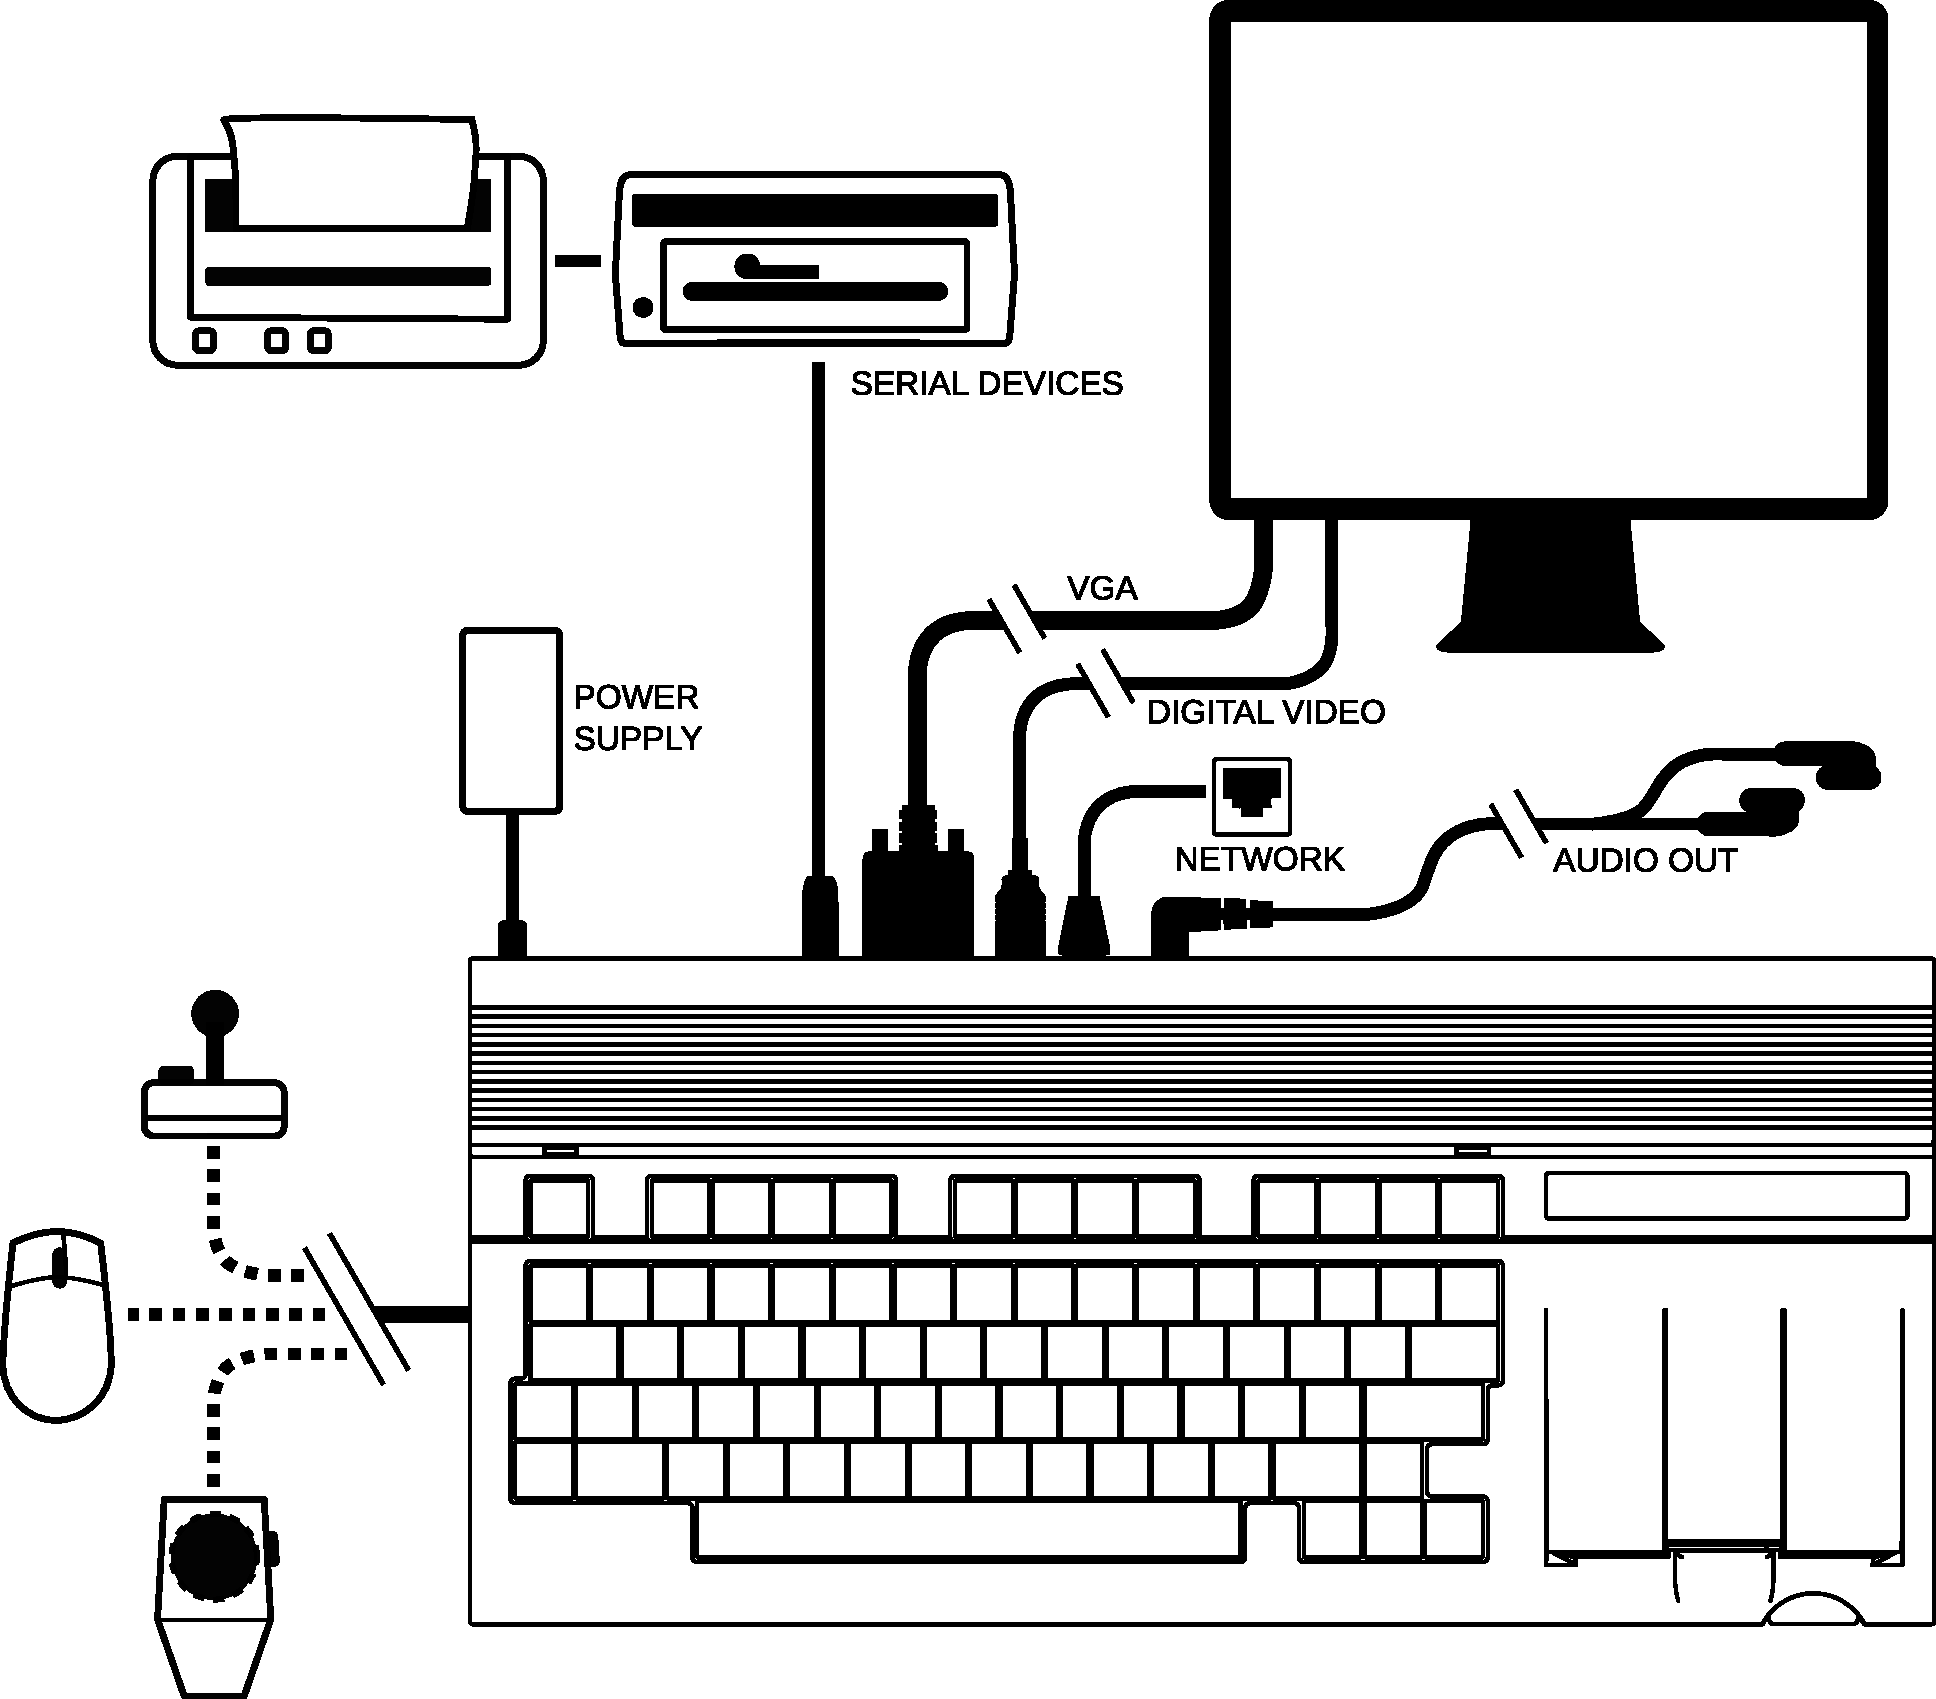
\includegraphics[width=\linewidth]{images/illustrations/mega65-top.pdf}

To connect your MEGA65 to a display:

\begin{enumerate}
	\item Connect the power supply to the power supply socket of the MEGA65.
	\item If you have a VGA monitor and a VGA cable, connect one end to the VGA port of the MEGA65 and the other end into your VGA monitor.
	\item If you have a TV or monitor with a compatible Digital Video connector, connect one end of your cable to the Digital Video port of the MEGA65, and the other into the Digital Video port of your monitor. If you own a monitor with a DVI socket, you can use a Digital Video to DVI adapter.
\end{enumerate}

\newpage
\section{Optional Connections}
\index{Connections!IEC}
\index{SD Cards!Locations}
\begin{enumerate}
	\item The MEGA65 includes an internal 3.5" floppy disk drive. You can also connect older Commodore{\textregistered} IEC serial floppy drives to the MEGA65, such as the Commodore 1541, 1571 or 1581. To use these drives, connect one end of an IEC cable to the Commodore floppy disk drive and the other end to the Disk Drive socket of the MEGA65. You can also connect SD2IEC devices and Pi1541's. It is also possible to daisy-chain additional floppy disk drives or Commodore compatible printers.
	\item You can connect your MEGA65 to an Ethernet network using a standard Ethernet cable.
	\item For enjoying audio from your MEGA65, you can connect a 3.5mm audio jack cable to an audio amplifier or speaker system. If your system has RCA connectors you will need a 3.5mm audio jack to twin RCA adapter cable. The MEGA65 also has a built-in amplifier to allow the use of headphones.
	\item A microSD card, type SDHC between 4GB and 32GB, can be inserted into the external microSD card slot at the rear of the MEGA65. For more information on using the microSD card slot, see ``Introducing SD Cards'' on page \pageref{sec:introducing-sd-cards}.
\end{enumerate}

\index{Real-Time Clock!Installing the Battery}
\subsection{Installing the Real-Time Clock Battery}

The MEGA65 includes a Real-Time Clock, which is used to display the time and date on the startup screen, to add timestamps to files that the MEGA65 writes to your SD cards, and by the {\bf DT\$} and {\bf TI\$} BASIC65 variables. This clock utilises a CR2032 coin-cell battery\footnote{Early models of MEGA65 with the "R3A" board revision used a battery of type CR1220 for the Real-Time Clock. Revisions "R5" and later, which began shipping in late 2023, use a CR2032 battery.} to keep time when the MEGA65 isn't switched on. The MEGA65 does not include a battery in order to avoid issues related to shipping batteries internationally.

To install the battery, use a Phillips-head screwdriver to open the case, exposing the motherboard. The case is held together with three screws, all of which are along the bottom of the front side of the case. Once the screws have been removed, carefully lift the top half of the case. Note the orientation of the keyboard connector, then disconnect it.

The battery is located between the controller ports and the keyboard connector.

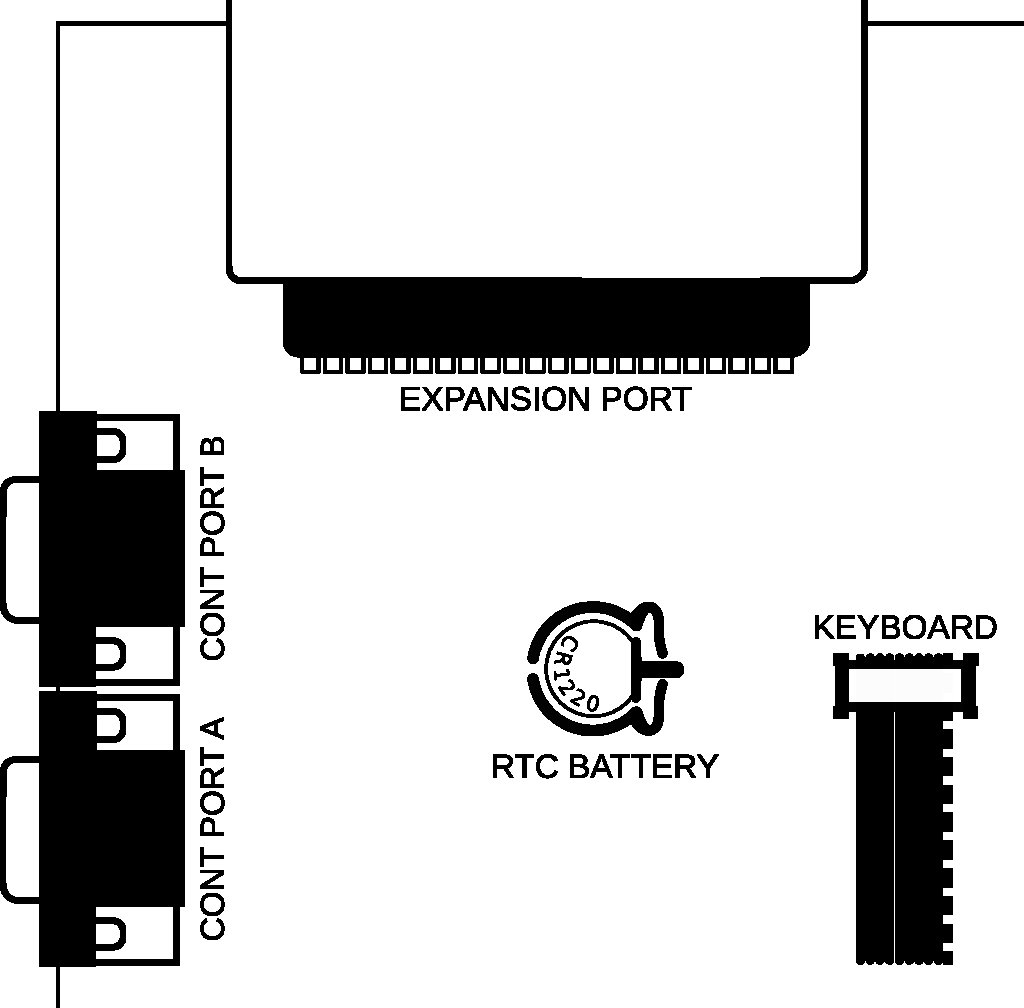
\includegraphics[width=10cm]{images/illustrations/rtc-battery-location.pdf}

If you are removing an existing battery, push the battery release lever on the bottom (flat-sided) side of the battery socket away from the battery to remove it. Insert the new battery with the side labelled {\bf +} facing up, and press it into place.

Once you have re-assembled your MEGA65, you can set the time in the Configure menu. For more information on how to set the Real-Time Clock, refer to the Configuration Utility section on page \pageref{sec:configuration-utility}.


\newpage

\section{Switching the MEGA65 on for the First Time}
\label{onboarding}

Switch the MEGA65 on using the power switch on the left-hand side of the computer.

When you switch your MEGA65 on for the first time, it displays the initial configuration (``on-boarding'') screen. You can use this screen to set the time and date on the Real-Time Clock (if you have installed the CR2032 battery), change the video display mode, and test the audio. All of these settings can be changed later.

\begin{center}
  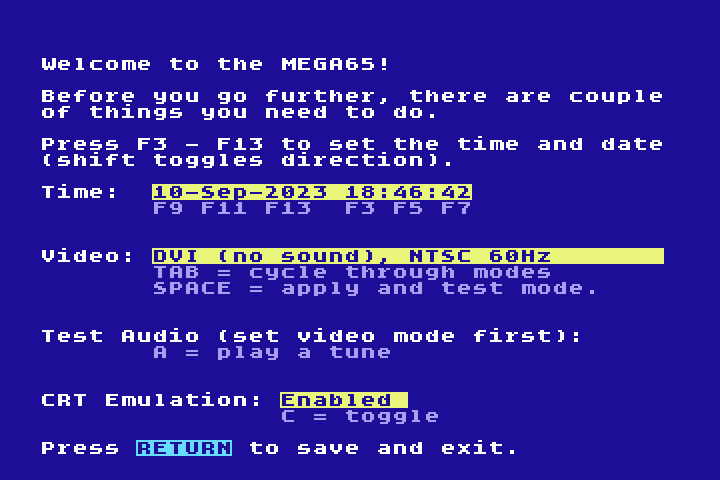
\includegraphics[trim= 10mm 15mm 10mm 10mm,clip,width=0.7\linewidth]{images/img011_final_boot_01.png}
\end{center}

For video display modes, you can select between PAL or NTSC emulation, and you can select whether your DVI display supports sound. If you are using the VGA video output, the DVI sound mode has no effect.

\underline{Note}: A DVI display that does not support sound will not work with the ``enhanced'' sound mode. With such a display, you must select a video mode with ``no sound,'' and connect a speaker to the 3.5 mm audio jack.

PAL and NTSC are analog video signal formats that affect the the resolution and vertical sync speed of the video output, even when using a modern digital display. Your display may support either mode, or it may only support one or the other. You can use this screen to test the modes with your display.

Select and test you video configuration. For example, press \specialkey{TAB} to switch to the ``PAL 50HZ'' mode.
\index{Display!Setting PAL/NTSC}
\begin{center}
  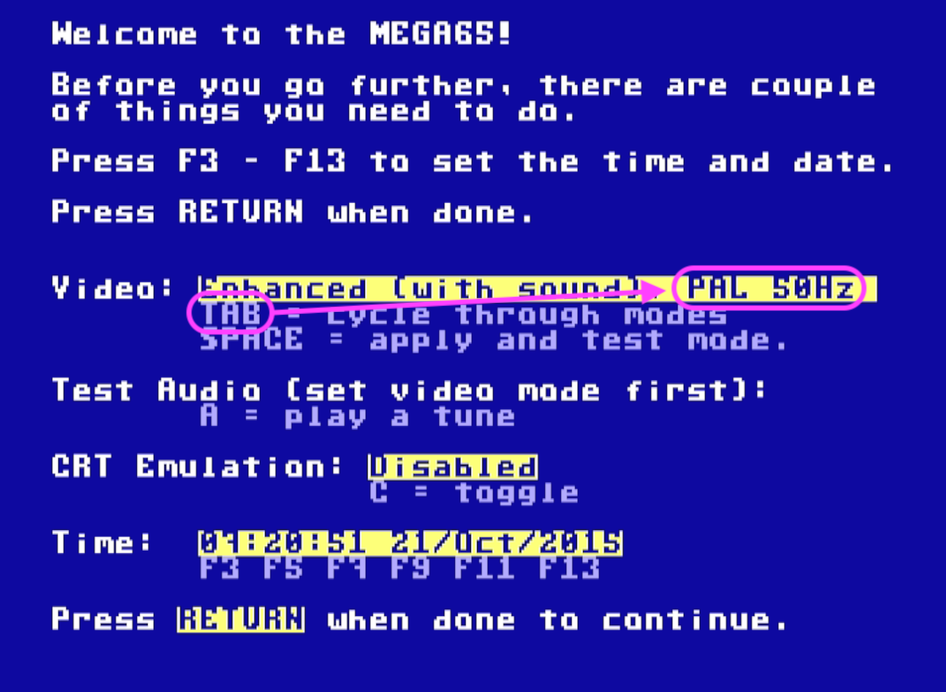
\includegraphics[width=0.7\linewidth]{images/img011_final_boot_02.png}
\end{center}

Press \megakey{SPACE} followed by \megakey{Y} to test the new video mode.

\begin{center}
  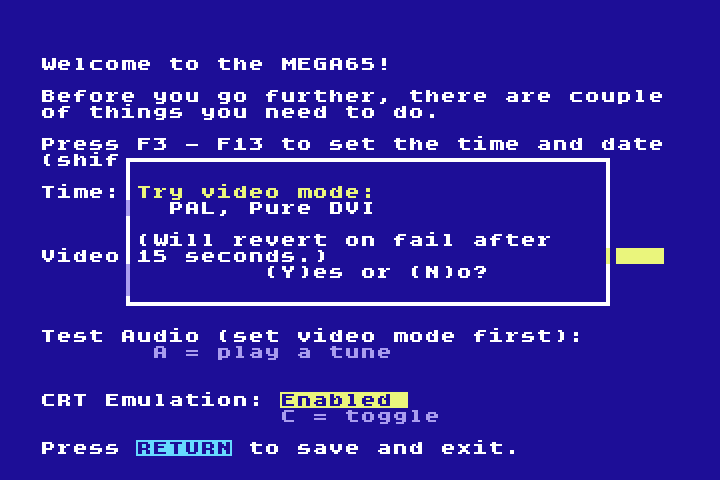
\includegraphics[trim= 15mm 10mm 10mm 15mm,clip,width=0.7\linewidth]{images/img011_final_boot_03.png}
\end{center}

Press \megakey{K} to keep the new video mode.

\begin{center}
  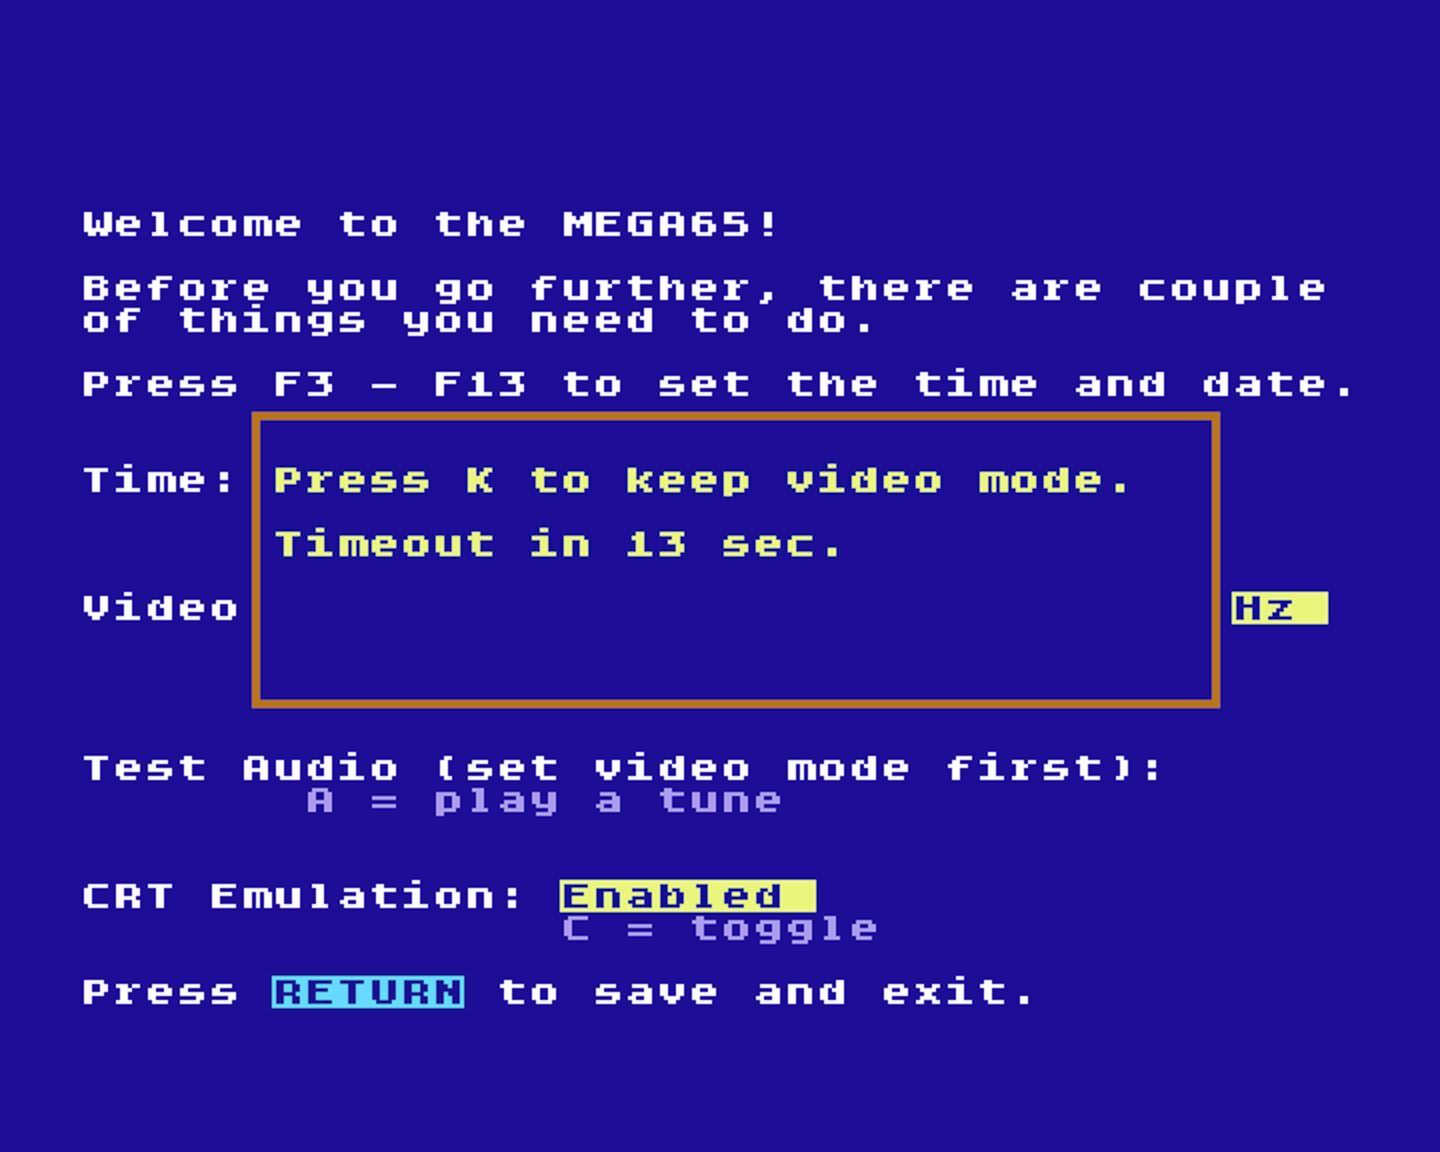
\includegraphics[trim= 20mm 20mm 10mm 25mm,clip,width=0.7\linewidth]{images/img011_final_boot_04.png}
\end{center}

Take this opportunity to test your sound set-up. Press \megakey{A} to play a sound.

The ``CRT emulation'' option is a fun choice when using a modern flat panel display. It adds vertical gaps between pixels to simulate the CRT raster line. Try it to see if you like it: press the \megakey{C} key to toggle it on and off.

Finally, press \specialkey{RETURN} to complete the configuration.

For more information about configuring your MEGA65, see chapter \vref{cha:configuringyourmega}.

\section{The Intro Disk}

After completing the on-boarding configuration, your MEGA65 starts the Intro Disk menu. The Intro Disk is a collection of software made by the MEGA65 community that demonstrates some of the capabilities of the computer. Take some time to browse the menus and try some of the demos. After each demo, press the reset button on the left-hand side of the computer to return to the Intro Disk menu.

\begin{center}
  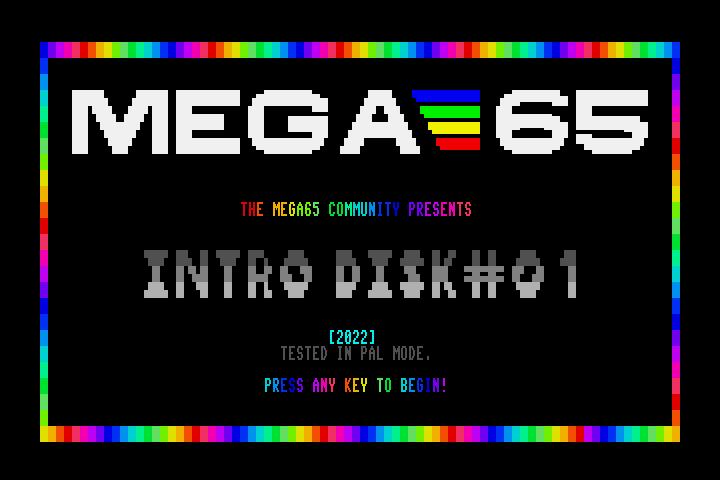
\includegraphics[width=0.7\linewidth]{images/demo_title.jpg}
\end{center}

By default, the Intro Disk menu opens each time you switch on the computer. Once you are more familiar with the MEGA65, you may wish to disable this. Press \megakey{D} at the Intro Disk menu to disable its auto-boot feature.

Press \megakey{X} to exit the Intro Disk menu and access BASIC 65. With the Intro Disk auto-boot feature disabled, the MEGA65 goes directly to BASIC 65 when you switch it on.

\begin{center}
  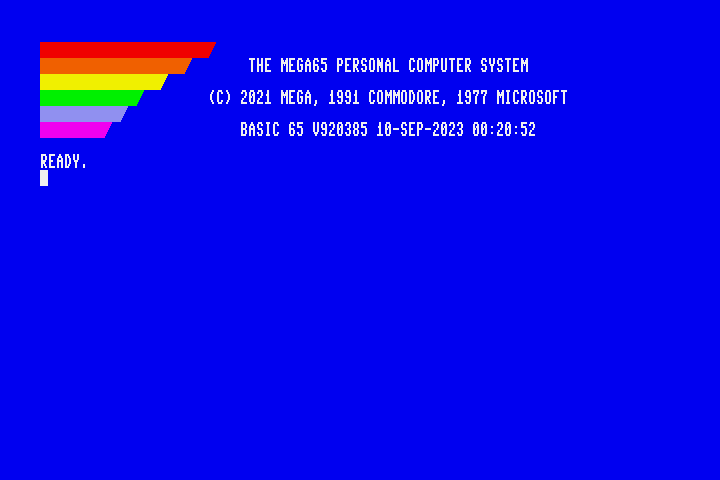
\includegraphics[trim=0 2cm 0 0,clip,width=0.7\linewidth]{images/img011_final_boot_06.png}
\end{center}

\subsection{The Cursor}

The flashing square underneath the \screentext{READY} prompt is called the cursor. The cursor indicates that the computer is ready to accept input. Pressing keys on the keyboard will print their respective characters onto the screen. The characters will be printed at the current cursor position, and the cursor will advance to the next position after every key press.

Here you can type commands, that can do things such as loading a program. You can also start entering program code!

\chapter{Getting Started}
\phantomsection
\section{Keyboard}
\label{cha:getting-started}

Now that everything is connected, it's time to get familiar with the MEGA65 keyboard.

You may notice that the keyboard is a little different from the keyboards used on computers today. While most keys will be in familiar positions, there are some specialised keys, and some with special graphic symbols marked on the front.

Here's a brief description of how some of these special keys function.

\subsection{Command Keys}

The Command Keys are: \specialkey{RETURN}, \specialkey{SHIFT}, \specialkey{CTRL}, \megasymbolkey, and \widekey{RESTORE}.

\subsubsection{RETURN}

Pressing \specialkey{RETURN} enters the information you have typed into the MEGA65's memory. The computer will either act on a command, store some information, or display an error message if you made a mistake.

\subsubsection{SHIFT}

The two \specialkey{SHIFT} keys are located on the left and the right. They work very much like the Shift key on a regular keyboard, however they also perform some special functions as well.

In upper case mode, holding down \specialkey{SHIFT} and pressing any key with two graphic symbols on the front prints the right-most graphic symbol to the screen. For example, \specialkey{SHIFT} and \megakey{J} prints the \graphicsymbol{J} character.

In lower case mode, pressing \specialkey{SHIFT} and a letter key prints the upper case letter on that key.

Finally, holding \specialkey{SHIFT} down and pressing a Function key accesses the function shown on the front of that key. For example: \specialkey{SHIFT} and \megakey{F1} activates \textbf{F2}.


\subsubsection{SHIFT LOCK}

In addition to \specialkey{SHIFT} is \specialkey{SHIFT\\LOCK}. Press this key to lock down the Shift function. Now any key you press while \specialkey{SHIFT\\LOCK} is illuminated prints the character to the screen as if you were holding down \specialkey{SHIFT}. This includes special graphic characters.

\subsubsection{CTRL}

\specialkey{CTRL} is the Control key. Holding down \specialkey{CTRL} and pressing another key allows you to perform Control Functions. For example, holding down \specialkey{CTRL} and one of the number keys allows you to change text colours. The colour that is printed at the top row on the front of the number key will be used.

There are some examples of this in \bookvref{sec:screen-editor}, and all of the Control Functions are listed in \bookvref{appendix:controlcodes}.

If a program is being LISTed to the screen, holding down \specialkey{CTRL} slows down the display of each line.

Holding \specialkey{CTRL} and pressing \megakey{*} enters the Matrix Mode Debugger (refer to the {\bf MEGA65 Book} for more details).

\subsubsection{RUN STOP}

Normally, pressing \specialkey{RUN STOP} stops the execution of a program. Holding \specialkey{SHIFT} while pressing \specialkey{RUN STOP} loads the first program from disk.

Programs are able to disable \specialkey{RUN STOP}.

You can boot your MEGA65 into the Machine Code Monitor by holding down \specialkey{RUN STOP} and pressing reset on the left-hand side.

\subsubsection{RESTORE}

The computer screen can be restored to a clean state without clearing the memory by holding down \specialkey{RUN STOP} and pressing \widekey{RESTORE}. This combination also resets operating system vectors and re-initialises the screen editor, which makes it a handy combination if the computer has become a little confused.

Programs are able to disable this key combination.

You can also enter the Freeze Menu by holding \widekey{RESTORE} down for more than one second. From there you can access the Machine Code Monitor.

\newpage

\subsubsection{THE CURSOR KEYS}

At the bottom right-hand side of the keyboard are the cursor keys. These four directional keys allow you move the cursor to any position for on-screen editing.

The cursor moves in the direction indicated on the keys: \megakey{$\leftarrow$} \megakey{$\uparrow$} \megakey{$\rightarrow$} \megakey{$\downarrow$}.

However, it is also possible to move the cursor up by using \specialkey{SHIFT} and \megakey{$\downarrow$}. In the same way you can move the cursor left by using \specialkey{SHIFT} and \megakey{$\rightarrow$}.

You don't have to keep pressing a cursor key over and over. If you need to move the cursor a long way, you can keep the key pressed down. When you are finished, simply release the key.

\subsubsection{INSerT/DELete}

This is the INSERT / DELETE key. When pressing \specialkey{INST\\DEL}, the character to the left is deleted, and all characters to the right are shifted one position to the left.

To insert a character, hold \specialkey{SHIFT} and press \specialkey{INST\\DEL}. All the characters to the right of the cursor are shifted to the right. This allows you to type a letter, number or any other character at the newly inserted space.


\subsubsection{CLeaR/HOME}

Pressing \specialkey{CLR\\HOME} places the cursor at the top left-most position of the screen.

Holding down \specialkey{SHIFT} and pressing \specialkey{CLR\\HOME} clears the entire screen {\it and} places the cursor at the top left-most position of the screen.

\subsubsection{MEGA KEY}

\megasymbolkey or the MEGA key provides a number of different functions and can be used to launch special utilities.

Holding \specialkey{SHIFT} and pressing \megasymbolkey switches between lower and uppercase character modes.

Holding \megasymbolkey and pressing any key with two graphic symbols on the front prints the left-most graphic symbol to the screen.

Holding \megasymbolkey and pressing any key that shows a single graphic symbol on the front prints that graphic symbol to the screen.

Holding \megasymbolkey and pressing a number key switches to one of the colours in the second range, i.e., the colour that is printed at the bottom row on the front of the number key will be used.

Holding \megasymbolkey and pressing \specialkey{TAB} enters the Matrix Mode Debugger (refer to the {\bf MEGA65 Book} for more details).

Switching on the MEGA65 or pressing the reset button on the left-hand side while holding down \megasymbolkey switches the MEGA65 into C64-mode.

\subsubsection{NO SCROLL}
If a program is being LISTed to the screen, pressing \specialkey{NO\\SCROLL} freezes the screen output. This feature is not available in C64-mode.


\subsection{Function Keys}

There are seven Function keys available for use by software applications. \megakey{F1} \megakey{F3} \megakey{F5} \megakey{F7} \megakey{F9} \megakey{F11} and \megakey{F13} can be used to perform specific functions with a single press.

Hold \specialkey{SHIFT} to access \megakey{F2} through to \megakey{F14} as shown on the front of each Function key.

Only Function keys \megakey{F1} to \megakey{F8} are available in C64-mode.

\subsubsection{HELP}

\specialkey{HELP} can be used by software and also acts as \megakey{F15} / \megakey{F16}.

\subsubsection{ALT}

Holding \specialkey{ALT} down while pressing other keys can be used by software to perform specific functions. Not available in C64-mode.

Holding \specialkey{ALT} down while switching the MEGA65 on activates the Utility Menu. You can format an SD card, or enter the MEGA65 Configuration Utility to select the default video mode and change other settings, or to test your keyboard.

\subsubsection{CAPS LOCK}

\specialkey{CAPS\\LOCK} works similarly to \specialkey{SHIFT\\LOCK} in C65 and MEGA65-modes, but only modifies the letter keys.
Also, holding \specialkey{CAPS\\LOCK} down forces the processor to run at the maximum speed. This can be used, for example,
to speed up loading from the internal disk drive or SD card, or to greatly speed up the de-packing process after a program is run.
This can reduce the loading and de-packing time from many seconds to as little as a fraction of a second.

\chapter{Configuring your MEGA65}
\label{cha:configuring}

\section{Important Note}

For your convenience, your MEGA65 comes with an SD card with all of the essential
files already on it, so you may prefer to skip this section and jump straight to
the on-boarding section on page \pageref{onboarding}.

Alternatively, you're welcome to read this section and familiarise
yourself on how your SD card was prepared.

{\bf Do not format the SD card that came with your MEGA65}.
If you want to create a new bootable SD card, please use another one,
and keep the SD card that came with your MEGA65 as a safety backup.

\section{Formatting SD cards}
\index{SD Cards!Formatting}
The MEGA65 has two SD card slots: A full-size SD card slot inside, under
the trap-door, and a microSD size slot on the rear.  The current version
of the MEGA65 firmware only supports the use of one SD card at a time.
If you have cards in both slots, the MEGA65 will default to the external slot. The exception to this is that the MEGA65's FDISK/FORMAT
utility can access both, allowing you to select which SD card to format or
repair.

If you wish to use a different SD card to the pre-configured one supplied with your MEGA65, the new SD card must be formatted first.

{\bf This must be done on the MEGA65, not on a PC or other computer.}

{\em Only use SDHC cards. Older SD cards (typically with
  a capacity of <4GB) will not work. Newer SDXC cards with
  capacities greater than 32GB may or may not work. We would
  appreciate hearing your experience with such cards. It is unimportant
  as to which file-system is currently on the card, as the MEGA65
  FDISK/FORMAT utility will completely reformat the card.}

There are several reasons for this: First, to fit the most
features into the MEGA65's small operating system, it is
particular about the FAT32 file system it uses. Second, only the
MEGA65 FDISK/FORMAT utility can create a MEGA65 System Partition. The
MEGA65 System Partition holds non-volatile configuration settings for
your MEGA65, and also contains the freeze slots that make it easy to
switch between MEGA65 programs and games.

Formatting an SD card on the MEGA65 is easy. Switch the MEGA65 on while holding \specialkey{ALT} down.

This will present the MEGA65 Utility Menu, which contains a
selection of built-in utilities, similar to the following:

%\begin{wrapfigure}{l}{0.7\textwidth}
\begin{center}
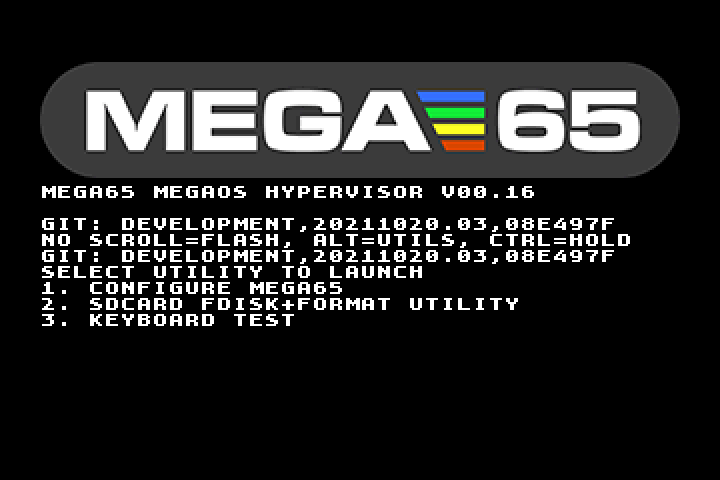
\includegraphics[width=0.7\textwidth]{images/ss-utilmenu.png}
\end{center}
%\end{wrapfigure}

Note that the Utility Menu is always accessible, even if no SD card is present in both the internal and external slots.

The exact set of utilities
depends on the model of your MEGA65 and the version of the MEGA65
factory core which it is running. However, all versions include both
the MEGA65 FDISK/FORMAT utility (which is called \screentext{SDCARD FDISK+FORMAT UTILITY} in the screenshot above),
and the MEGA65 Configure utility.
Most models also include a keyboard test utility, that you can use
to test that your keyboard is functioning correctly.  This is
the same utility used in the factory when testing brand
new keyboards.

Select the number that corresponds to the FDISK/FORMAT utility.  This
will typically be 2.  The FDISK utility will start, and attempt to
detect the size of all SD cards you have installed.  If you have both
an internal and external SD card installed, it will allow you to
choose which one you wish to format. The internal SD card is bus 0,
and the external microSD card is bus 1. Note that the MEGA65 will
always attempt to boot from the external microSD card if one is
present.

For safety, when formatting we {\em strongly} recommend
that you remove any SD card or microSD card that you do not intend to
format, so that you do not accidentally destroy any data.  This is
because formatting an SD card on the MEGA65 cannot be undone, and
all data currently on the SD card {\em will be lost}.  If you
have files or data on the SD card that you wish to retain, you
should first back them up.  The contents of the FAT32
partition can be easily backed up by inserting the SD card into
another computer.  The contents of the MEGA65 System Partition,
including the contents of freeze slots requires the use of specialised
software.

You should aim to back up valuable data from your
MEGA65 on a regular basis, especially while the computer remains under
development.  While we take every care to avoid data corruption or
other mishaps, we cannot guarantee that the MEGA65 is free of bugs in
this regard.

If you have only an internal SD card, you might see a
display similar to the following:

\begin{center}
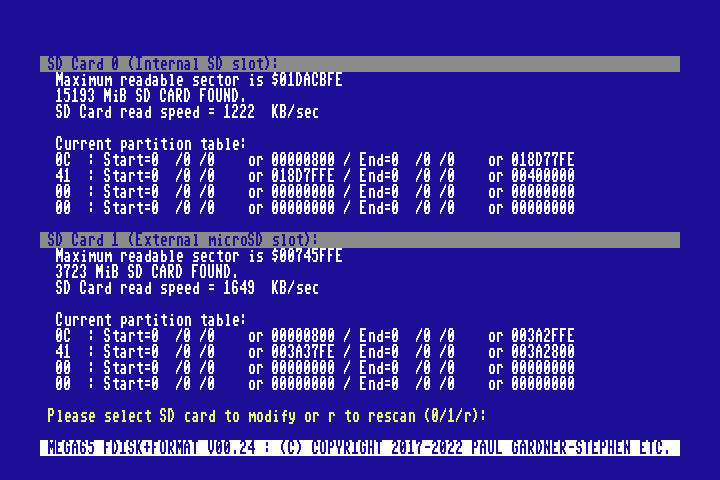
\includegraphics[trim= 10mm  7mm 10mm 10mm,clip,width=0.7\linewidth]{images/ss-m65fdisk-busselect.png}
\end{center}

Once you have selected the bus, the FDISK/FORMAT utility will ask you to confirm that you wish to delete everything:

\begin{center}
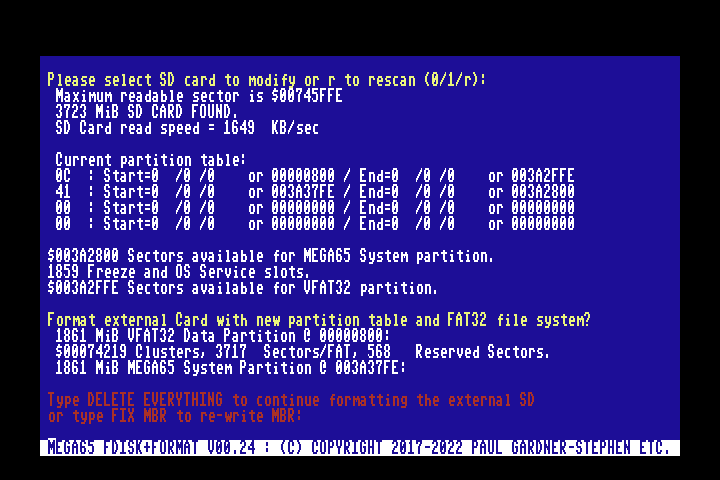
\includegraphics[trim= 10mm  7mm 10mm 15mm,clip,width=0.7\linewidth]{images/ss-m65fdisk-typesomething.png}
\end{center}

To avoid accidental loss of data, you must type \screentext{DELETE EVERYTHING} in capitals and press \specialkey{RETURN}. Alternatively, switch the MEGA65 off and on to abort this process without causing damage to your data.

It is also possible to attempt a recovery from a lost Master Boot Record error (also known as the Boot Sector), by typing \screentext{FIX MBR} instead.

The aim here is to have a correctly formatted SD card with all of the essential files stored on it so the MEGA65 can properly boot.
When switching on, the MEGA65 will search for, and boot using these files:
\begin{itemize}
\item {\tt FREEZER.M65} (Freeze Menu program)
\item {\tt AUDIOMIX.M65} (Freeze Menu audio mixer utility)
\item {\tt C64THUMB.M65} (C64 thumbnail image used in freezer)
\item {\tt C65THUMB.M65} (C65 thumbnail image used in freezer)
\item {\tt MEGA65.ROM}   (128KB ROM file)
\item {\tt MEGA65.D81} (Disk image)
\end{itemize}

Straight out of the box, the MEGA65 will only have one SD card installed, accessible via the trap-door under the case. This SD card contains all of the essential files needed to properly boot up.
If an external microSD card is also detected during boot up, the MEGA65 will give it higher priority, and will try to boot from it instead.
This means that the external microSD card needs to have the essential files on it, otherwise the MEGA65 will not boot up properly and will fall back to loading the OpenROM, which does not support all MEGA65 features.
In general, if your MEGA65 cannot boot properly and falls back to OpenROM, your boot-up screen will look similar to this:

\begin{center}
\includegraphics[trim=0 8cm 0 0,clip,width=0.7\linewidth]{images/mega65_OpenROM_boot_noSD.png}
\end{center}


\section{Installing ROM and Other Support Files}
\label{sec:installingrometc}

The MEGA65 FDISK/FORMAT utility will add a copy of the Open ROMs project's C64-compatible ROM
to your SD card, and will name it {\tt MEGA65.ROM}.

For MEGA65 owners, we have replaced this file with the latest ROM from the 'Closed ROMs'
project. It provides many improvements over the original/incomplete C65 ROMs. It contains
the operating system, BASIC 65, CBDOS and the machine language monitor BSMON.
This ROM is developed especially for the MEGA65 and can be
identified by the version number \screentext{92XXXX}.

However, you may have other ROMs that you wish to
use on your MEGA65.
You can copy as many of these as you wish onto the
SD card, just make sure that they have the {\tt .ROM} file extension.  The default ROM
should be called "{\tt MEGA65.ROM}". These files
must be 128KB in size, and use the same internal format as the ROMs
intended for the C65.  This means that the C64-mode KERNAL must be
placed at offset \$E000, a C65-mode BASIC at \$A000, and a suitable
character set at \$D000.

You can optionally name your alternate ROMs as {\tt MEGA65x.ROM}, replacing {\tt x} with a number from 0 to 9.
This allows you to quickly boot-up to your alternate ROMs by holding down a number from \megakey{0} to \megakey{9} prior
to switching on your MEGA65.

Other important support files include {\tt FREEZER.M65} and {\tt AUDIOMIX.M65}, which
allow you to use the MEGA65's integrated Freezer. More details are provided in the
'Floppy Disks, D81 Images, and the Freezer' chapter on page \pageref{cha:freezer}.

\subsection{ROM File}

\textbf{Original C65 ROMs}

You may want to source your own C65 ROM via other means.
There were many different versions created during the development of the Commodore 65,
and the MEGA65 can use any of them.  However, they will not support the advanced
features of the MEGA65, and are incomplete and buggy, as development on them ceased
due to Commodore abandoning the C65 project.

\textbf{MEGA65 Closed ROMs}

There are newer versions of the MEGA65 Closed ROM under development. These ROMs improve upon the original C65 ROMs and make better use of the extra hardware capabilities that the MEGA65 has over the original C65 hardware. These ROMs are available via the filehost (\url{https://files.mega65.org}), but only to owners of the MEGA65, who will need to login to the filehost with their credentials in order to download it. It can be located by visiting the \textbf{Files} tab and searching for "\textbf{kernal rom}":

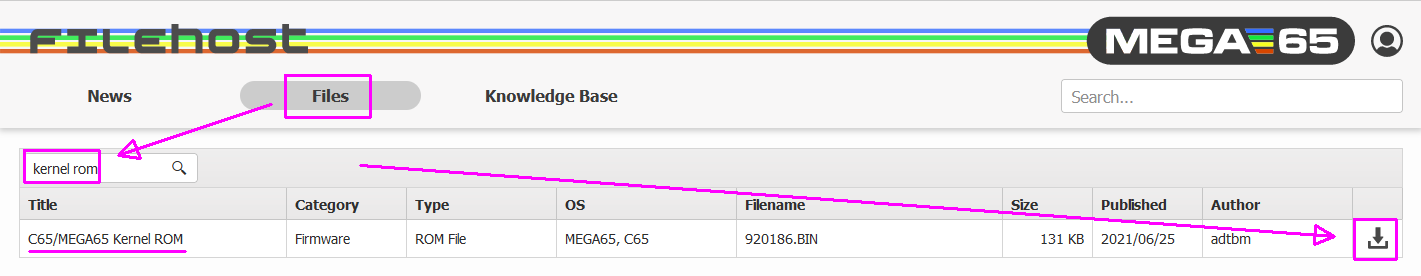
\includegraphics[width=\linewidth]{images/latest_closed_rom.png}

\textbf{MEGA65 ROM diff files}

If you have sourced your own {\tt 911001.bin} C65 ROM and would like to patch it to the latest MEGA65 closed ROM,
we do provide patches, as the additional improvements we have made to the closed rom are open source.
These diff files are available at \url{http://mega65.org/rom-diffs}

\textbf{MEGA65 Open ROMs}

Another available option is to make use of \textbf{MEGA65 Open ROMs}. The latest version of this is always downloadable from either of the following urls:

\begin{itemize}
  \item \url{http://mega65.org/open-roms}
  \item \url{https://github.com/MEGA65/open-roms/raw/master/bin/mega65.rom}
\end{itemize}


\subsection{Support Files}

For official owners of the MEGA65 (both the devkit and the final product), visit the following url and log in with the user credentials you have been provided. This will take you to the MEGA65 Filehost location where the \textbf{MEGA65 SD card essentials} download page is located. Click the \textbf{Download} link to retrieve the latest \textbf{SD essentials.rar} file.

\url{http://mega65.org/sdcard-files}

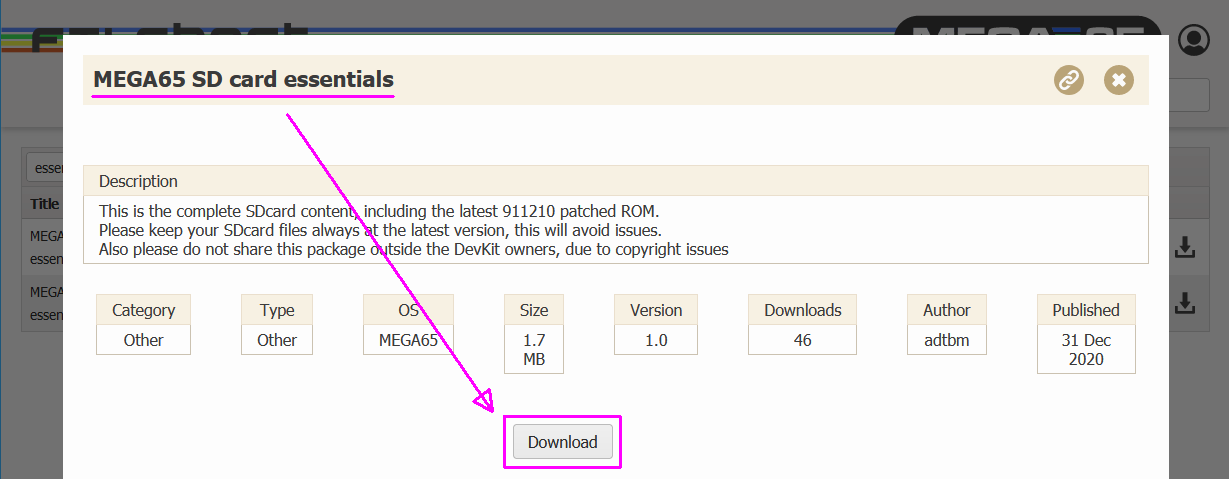
\includegraphics[width=\linewidth]{images/latest_support_files_with_closedrom.png}

Note that this link is only available to official owners of the MEGA65 product, as the fileset also contains the licensed closed-source {\tt MEGA65.ROM} file.
\ifdefined\printmanual
\else
For Nexys board owners in search of a similar fileset (without the ROM), visit the following url instead: \url{http://mega65.org/sdcard-norom}
\fi

This will take you to the MEGA65 Filehost location where the \textbf{MEGA65 SD card essentials - No ROM} download page is located. Click the \textbf{Download} link to retrieve the latest \textbf{SD essentialsNoROM.rar} file.

Note that while this fileset does not contain a ROM, there are future plans for it to include the freely available ROM from the Open ROMs project.

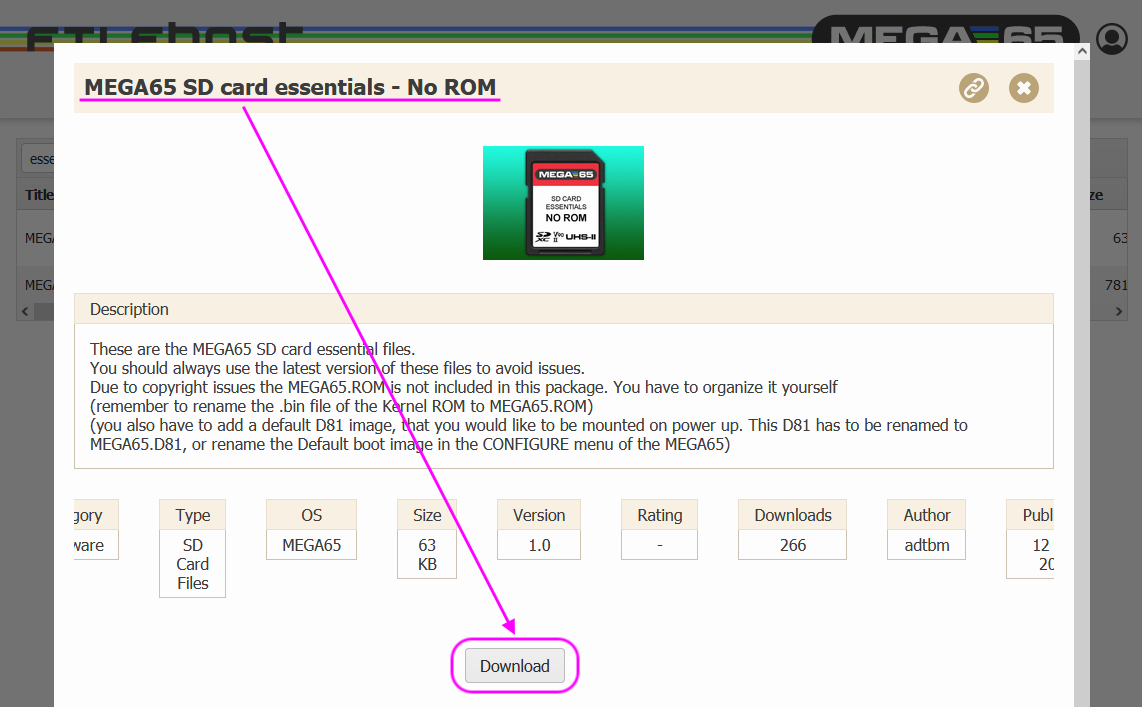
\includegraphics[width=\linewidth]{images/latest_support_files.png}

\section{On-boarding}
\label{onboarding}

On first launch of your MEGA65, you will see the on-boarding screen:

\begin{center}
  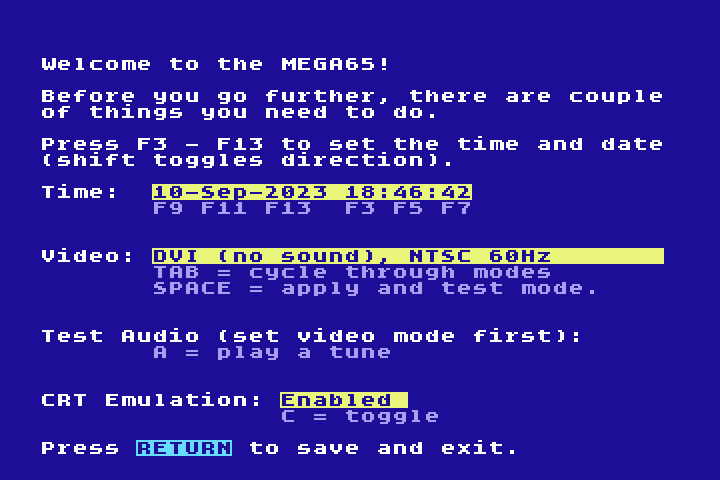
\includegraphics[trim= 10mm 15mm 10mm 10mm,clip,width=0.7\linewidth]{images/img011_final_boot_01.png}
\end{center}

Here you can select and test you screen configuration.

For example, press \specialkey{TAB} to switch to PAL 50HZ:
\index{Display!Setting PAL/NTSC}
\begin{center}
  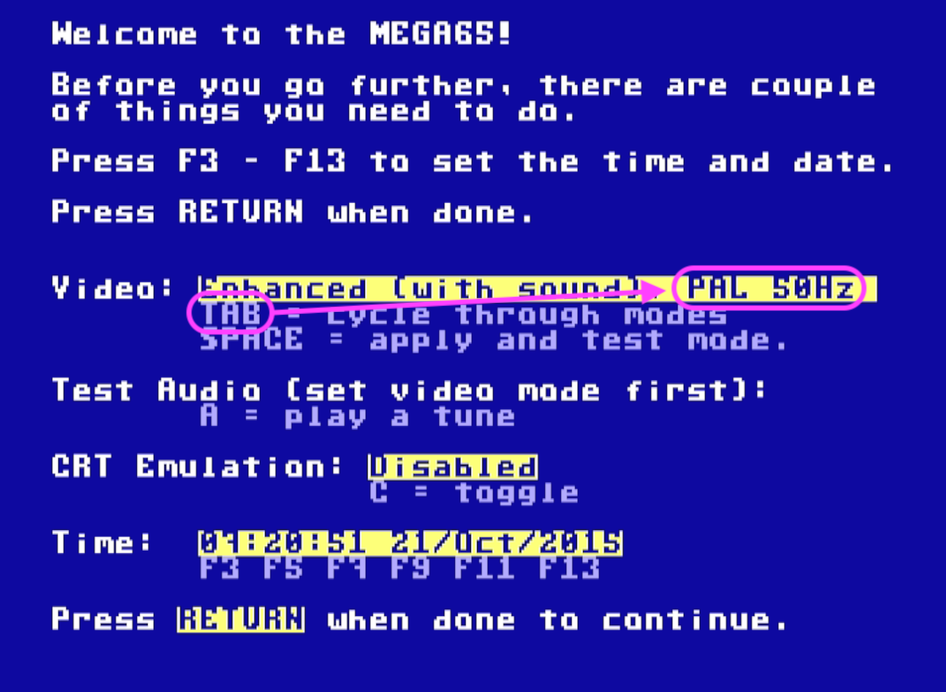
\includegraphics[width=0.7\linewidth]{images/img011_final_boot_02.png}
\end{center}

Then press \specialkey{RETURN} , followed by \megakey{Y} to test the new video mode:

\begin{center}
  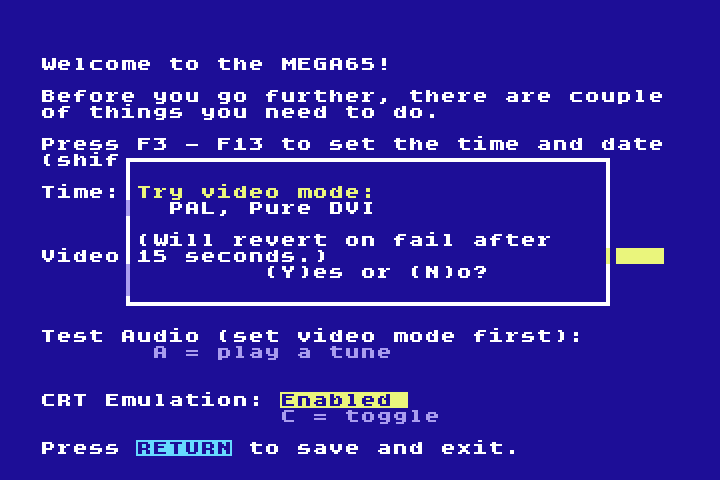
\includegraphics[trim= 15mm 10mm 10mm 15mm,clip,width=0.7\linewidth]{images/img011_final_boot_03.png}
\end{center}

Press \megakey{K} to keep the new video mode:

\begin{center}
  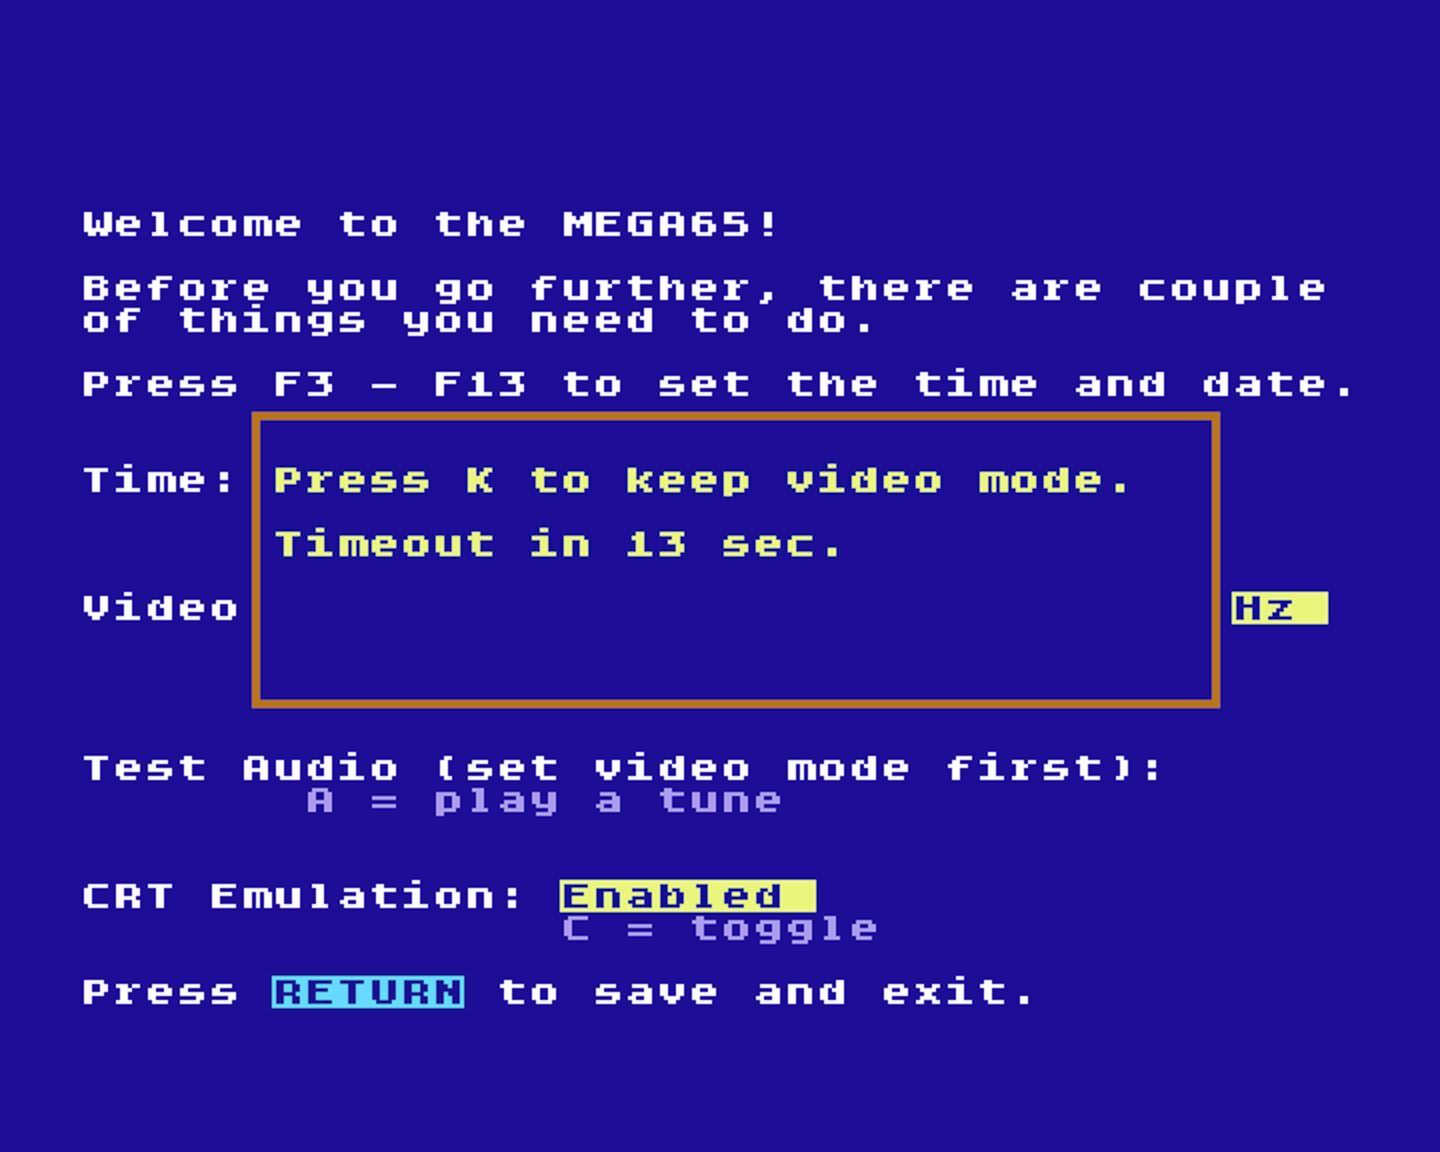
\includegraphics[trim= 20mm 20mm 10mm 25mm,clip,width=0.7\linewidth]{images/img011_final_boot_04.png}
\end{center}

Press \specialkey{RETURN} to complete the configuration:

\begin{center}
  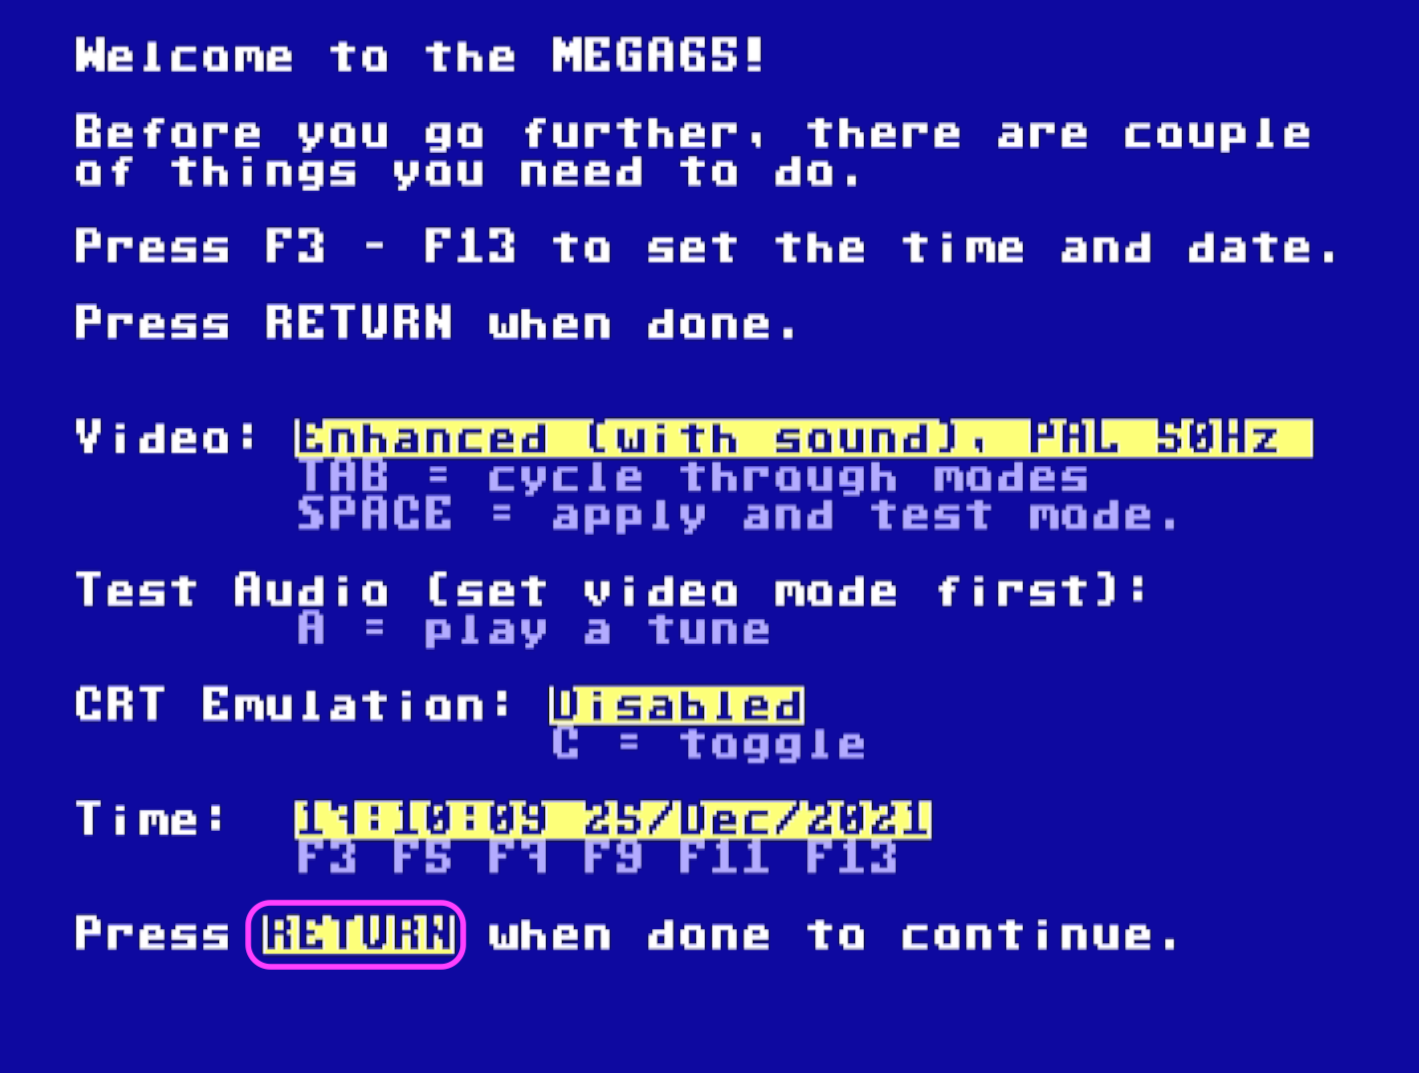
\includegraphics[trim= 6mm 6mm 6mm 6mm,clip,width=0.7\linewidth]{images/img011_final_boot_05.png}
\end{center}

\ifdefined\printmanual
\else
\textcolor{red}{\underline{Note for Nexys4 board users}: \\
\\
  At this very specific step, the board is supposed to reboot and display the main MEGA65 screen. If the board does not reboot and the screen remains black, then switch power to the board off then on again.}
\fi

After the MEGA65 reboots you will be greeted with the main MEGA65 screen:

\begin{center}
  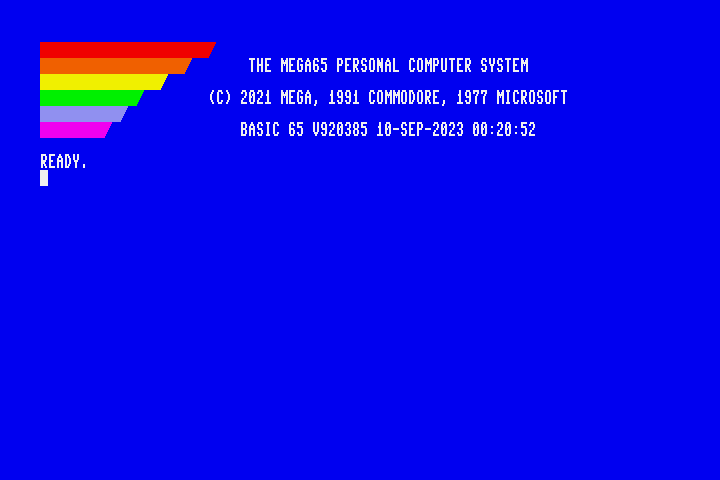
\includegraphics[trim=0 2cm 0 0,clip,width=0.7\linewidth]{images/img011_final_boot_06.png}
\end{center}

\section{Configuration Utility}
\label{sec:configuration-utility}

The configuration utility for the MEGA65 has a similar purpose to the BIOS on a PC, which is to allow you to control certain default behaviours of your MEGA65. However, rather than storing the configuration data in
battery-backed RAM, the MEGA65 stores this data on sector 1 of the SD card. If you switch SD cards, you will change the configuration data.

  To enter the configuration utility, switch the MEGA65 on while
  holding \specialkey{ALT} down.  This will show the utility menu,
  similar to the following:

\begin{center}
  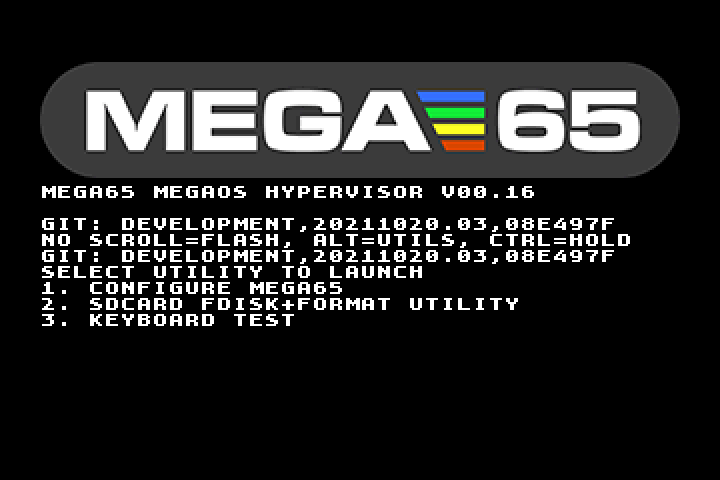
\includegraphics[width=0.7\linewidth]{images/ss-utilmenu.png}
\end{center}

%\begin{minipage}{\linewidth}
  Next, press the number corresponding to the \screentext{CONFIGURE MEGA65} item.  The MEGA65
  Configuration Utility will launch, showing a display similar to
  the following:

%  \vspace{5mm}
\begin{center}
  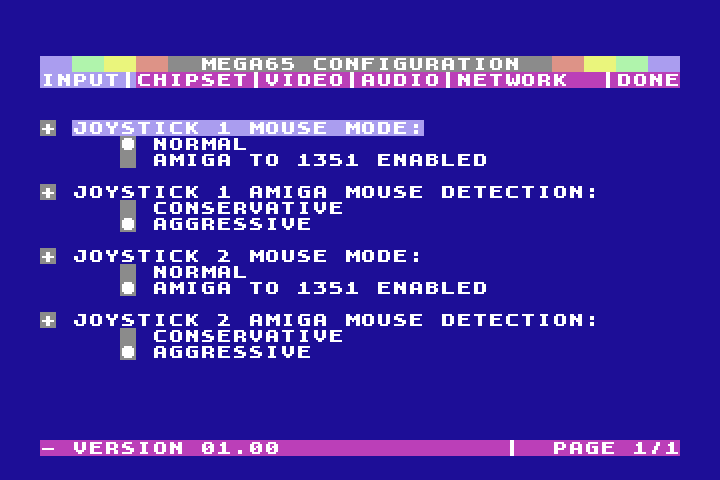
\includegraphics[width=0.7\linewidth]{images/ss-m65config-1.png}
\end{center}
%\end{minipage}

%\begin{minipage}{\linewidth}
  If your MEGA65's System Partition is corrupted, you may be
  prompted to press \megakey{F14} to correct this, (i.e., hold \specialkey{SHIFT} and press
  \megakey{F13}), with a display similar to the following:

%  \vspace{5mm}
\begin{center}
  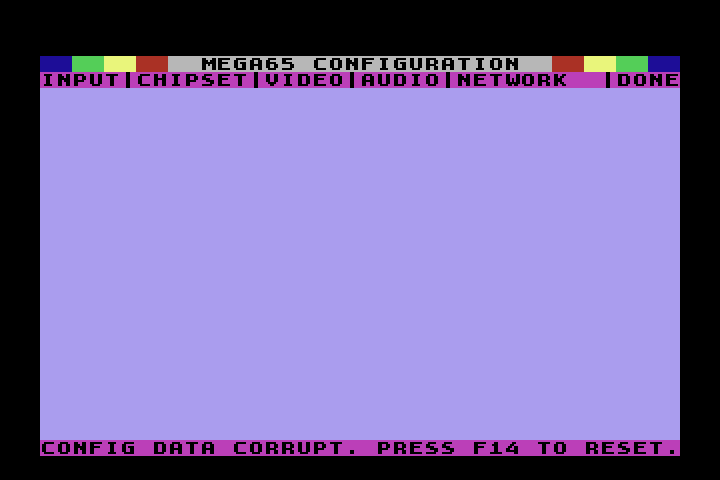
\includegraphics[width=0.7\linewidth]{images/ss-m65config-corrupt.png}
\end{center}
%\end{minipage}

To correct this error, press \megakey{F14}. Next, press \megakey{F7} to save the reset configuration, otherwise the reset data will not be saved to the MEGA65 System
Partition.

Once you have dismissed that display, or if your MEGA65 System Partition is not corrupt, you can begin exploring and adjusting various settings. The program can be controlled using the keyboard, or optionally, a 1351 or Amiga\texttrademark{} mouse.

You can advance screens by pressing \megakey{F1}, or use \megakey{F2} to navigate in the opposite direction. Use \megakey{$\leftarrow$} and \megakey{$\rightarrow$} to navigate between screens.

Use \megakey{$\uparrow$} and \megakey{$\downarrow$} to select an item.

Press \specialkey{RETURN} or \megakey{SPACE} to toggle a setting, or to change a text or numeric value. The black circle next to an option indicates the current selection.

  When you have finished, press \megakey{F7} to see the
  options for saving the changes. This will give you four options:

\begin{center}
  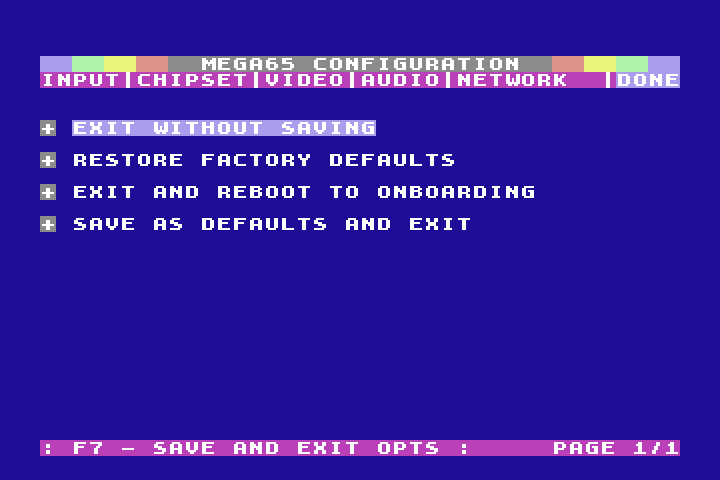
\includegraphics[width=0.7\linewidth]{images/ss-m65config-save.png}
\end{center}

\begin{itemize}
  \item \screentext {EXIT WITHOUT SAVING} abandons any changes made in the MEGA65 Configure utility and exits.
  \item \screentext {APPLY AND TEST SETTINGS NOW} uses the current settings immediately but does not exit. This is helpful to test compatibility of your TV or monitor with PAL or NTSC video modes. If you still see your display after applying a change, it is safe to save those settings.
  \item \screentext {RESTORE FACTORY DEFAULTS} resets the MEGA65 configuration settings to the factory defaults. It will randomly select a new MAC address for models that include an internal Ethernet adaptor. If you wish to commit these changes, you must still save them.
  \item \screentext {SAVE AS DEFAULT AND EXIT} commits changes made to the SD card. These changes will be used when the MEGA65 is switched on.
\end{itemize}

\subsection{Input Devices}

\begin{center}
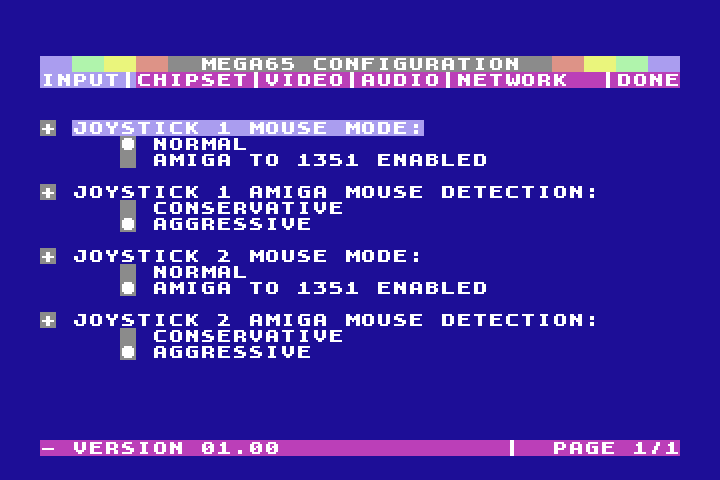
\includegraphics[width=0.7\linewidth]{images/ss-m65config-1.png}
\end{center}

\begin{itemize}
  \item \screentext{JOYSTICK 1 AMIGA MOUSE MODE} allows either \screentext{NORMAL} operation,
  where software will see it as an Amiga mouse or \screentext{1351 EMULATION} mode, where the MEGA65 translates the Amiga mouse's movements into 1351 compatible signals. This allows you to use an Amiga mouse with existing C64/C65 software that expects a 1351 mouse.
  \item \screentext{JOYSTICK 1 AMIGA MOUSE DETECTION} can be set to \screentext{CONSERVATIVE} or \screentext{AGGRESSIVE}. If you use an Amiga mouse and it fails to move smoothly in all directions, you may set it to \screentext{AGGRESSIVE}. Conversely, if you regularly use joysticks in the port, and have difficulties with the joystick input misbehaving, you might want to use the \screentext{CONSERVATIVE} option.
  \item \screentext{JOYSTICK 2 AMIGA MOUSE MODE} is identical to the first option, but for the second controller port. This allows you to have different settings for each port.
  \item \screentext{JOYSTICK 2 AMIGA MOUSE DETECTION} similarly provides the ability to separately control the Amiga mouse detection algorithm for the second controller port.
\end{itemize}


\subsection{Chipset}
\label{configuring-chipset}
\begin{center}
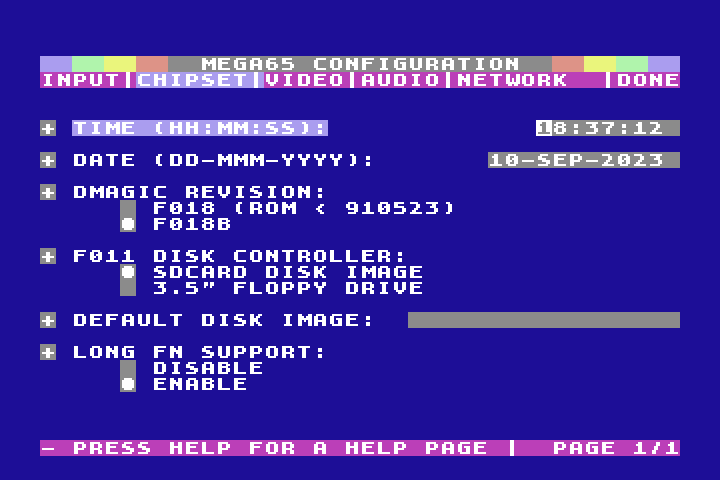
\includegraphics[width=0.7\linewidth]{images/ss-m65config-2.png}
\end{center}

\begin{itemize}
  \item \screentext{REAL-TIME CLOCK} allows setting the MEGA65's Real-Time
    Clock for those models that include one.  To set the clock or
    calendar, simply edit the field and press \specialkey{RETURN}.
    The display does not change while viewing this page, but if
    you use \megakey{$\leftarrow$} and \megakey{$\rightarrow$} to select another page and
    return to this page, the values will update if a Real-Time Clock
    is fitted and functioning.
  \item \screentext{DMAGIC REVISION} allows selecting the default mode of
    operation for the C65 DMAgic DMA controller.  This option is only
    required for ROMs not detected by the MEGA65's HYPPO Hypervisor.
    If you see screen corruption in BASIC,
    try toggling this option.
  \item \screentext{F011 DISK CONTROLLER}
    \index{Disk Drives!D81 Images}
    This option allows you to select whether the internal 3.5'' floppy
    drive functions using real diskettes, or whether it simply makes
    noises to add atmosphere when using D81 disk images from the SD
    card.  This merely sets the default option, and you can change
    this setting, or select a different disk image for use as either
    or both of the C65 3.5'' DOS based drives.
  \item \screentext{DEFAULT DISK IMAGE} allows you to choose the D81 disk image
    used with the internal drive, if the \screentext{F011 DISK CONTROLLER}
    option above is set to \screentext{USES SDCARD DISK IMAGE}. You can read more about
    D81 disk images on page \pageref{sec:d81-images}.
  \item \screentext{LONG FN SUPPORT} is a feature that is still under development
    at time of writing, and we suggest leaving it disabled for now until the feature
    matures in future bitstreams. Its aim is to provide long filename support for the
    SD card.
\end{itemize}

\subsection{Video}

\begin{center}
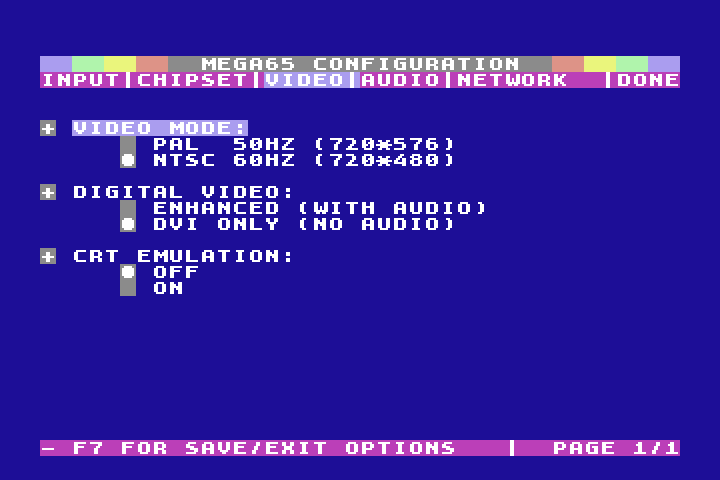
\includegraphics[width=0.7\linewidth]{images/ss-m65config-3.png}
\end{center}
\index{Display!Setting PAL/NTSC}
\begin{itemize}
  \item \screentext{VIDEO MODE} selects whether the MEGA65 starts in PAL or NTSC.    The MEGA65 supports true 480p NTSC and 576p PAL double-scan modes, with exact 60Hz / 50Hz frame-rates. This setting sets the default value, and the system can be switched between PAL and NTSC via the Freeze Menu, or under software control by MEGA65-enabled programs.
  \item \screentext{DIGITAL VIDEO} allows for selection between either \screentext{ENHANCED} video output containing audio, or \screentext{DVI ONLY} video output with no audio.
  \item \screentext{CRT EMULATION} selects whether CRT scanline emulation should be applied to the video output or not.
\end{itemize}

\subsection{Audio}

\begin{center}
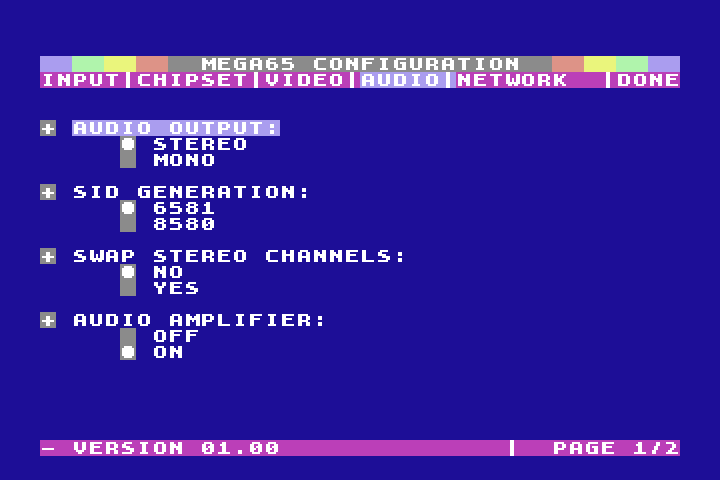
\includegraphics[width=0.7\linewidth]{images/ss-m65config-4.png}
\end{center}

\begin{itemize}
  \item \screentext{AUDIO OUTPUT} selects whether the SIDs and digital audio channels are combined to provide a monaural signal or whether the left and right tagged audio sources are separated to provide a stereo signal. This setting can be changed in the Audio Mixer of the Freeze Menu, or under the control of MEGA65-enabled software.
  \item \screentext{SWAP STEREO CHANNELS} allows switching the left and right-hand sides of the stereo audio output. This is useful for software that expects left and right SIDs to be at swapped addresses compared with the MEGA65 defaults.
  \item \screentext{DAC ALGORITHM} allows selecting between two different digital to analog conversion algorithms. Both options sound good and the selection is a personal preference.
  \item \screentext{AUDIO AMPLIFIER} allows enabling or disabling the audio amplifier contained in some models of the MEGA65. This option works for audio outputs, e.g., internal speaker or loud speaker.
\end{itemize}

\subsection{Network}

\begin{center}
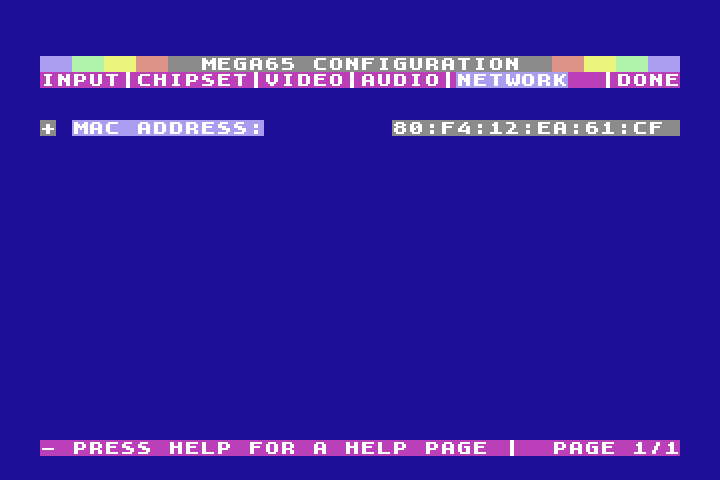
\includegraphics[width=0.7\linewidth]{images/ss-m65config-5.png}
\end{center}

\begin{itemize}
  \item \screentext{MAC ADDRESS} allows you to set the default MAC address of your MEGA65. This can be changed at run-time by MEGA65-enabled software.
\end{itemize}

% 2021-03-17 edits by SBC

\chapter{Upgrading the MEGA65}

\section{How a MEGA65 Can Be Upgraded}
\label{cha:cores}

The MEGA65 platform consists of three major components:

\begin{enumerate}
  \item The {\bf MEGA65 core},\index{Core} a description of the chipset to run on the FPGA
  \item The {\bf ROM},\index{ROM} code that defines the Commodore-style operating system (KERNAL) and BASIC
  \item {\bf System software} for features such as the Freezer menu\index{Freezer menu}
\end{enumerate}

You can upgrade these components as new releases are published. You can also replace one or more of these components individually. In the case of the core and ROM, you can even have multiple versions installed simultaneously and switch between them. For example, instead of the latest MEGA65 ROM, you can switch to the original Commodore 65 prototype ROM. Or, you could switch to another core that causes your MEGA65 hardware to behave like a different computer entirely, such as a Commodore 64 or a ZX Spectrum.

The ROM and system software are files that reside on the SD card, and upgrading them is as simple as replacing the files. To upgrade the core, you use a process to install a core file into the MEGA65's core flash memory. This chapter describes this process.

\subsection{What is a Core?}
\index{Core!definition}

The MEGA65 hardware architecture is based on a versatile chip called a ``Field Programmable Gate Array,'' or FPGA.\index{Field Programmable Gate Array (FPGA)} This is a special kind of computer chip that can be programmed to impersonate other chips. They do this by configuring a giant array of logic gates to reproduce circuits. FPGAs are not an emulation, but an electronic re-creation of other chips. FPGA code is sometimes referred to as {\em firmware,} a term you may recognize from modern computers and other devices.

Your MEGA65 was programmed at the factory to re-create a chipset designed by the MEGA65 team, based on the original Commodore 65. You can re-program the MEGA65 FPGA to upgrade to new versions of the MEGA65 chipset, or to replace the chipset with that of an entirely different computer!

Each possible chipset is known as a {\em core}. The MEGA65 can store up to eight cores, and you can switch between these cores by accessing a menu when you switch on the computer. You can also use this menu to load a new core from a file on the SD card, a process known as {\em flashing}.

Members of the MEGA65 community have made several useful and fun alternate cores for the FPGA hardware. \href{https://github.com/MJoergen/C64MEGA65}{{\em C64 for MEGA65}} by MJoergen and sy2002 re-creates the original Commodore 64 computer with a high degree of accuracy, perfect for running Commodore 64 games, demos, and applications. Other cores re-create the ZX Spectrum, the Game Boy, and even the original Galaga arcade machine hardware. The MEGA65 team believes that the FPGA is powerful enough to re-create nearly all 8-bit home computers, and likely some 16-bit computers and consoles such as the Commodore Amiga. The MEGA65 hardware design, board layout, FPGA core, and other information are all available for free under various open-source licenses, so anyone is free to create other cores for the MEGA65 hardware.

\section{Determining the Versions of Things}
\label{sec:versions}

All components of the MEGA65 platform have a version identifier. The MEGA65 can display the version identifiers for all of its components using the MEGA65 Information utility.\index{MEGA65 Information Utility}

To open the MEGA65 Information utility:

\begin{enumerate}
  \item Switch on the MEGA65, and allow it to boot to BASIC.
  \item Open the Freezer:\index{Freezer menu} press and hold \widekey{RESTORE} for one second then release it.
  \item Press \specialkey{HELP}. The MEGA65 Information utility will open.
\end{enumerate}

\begin{center}
  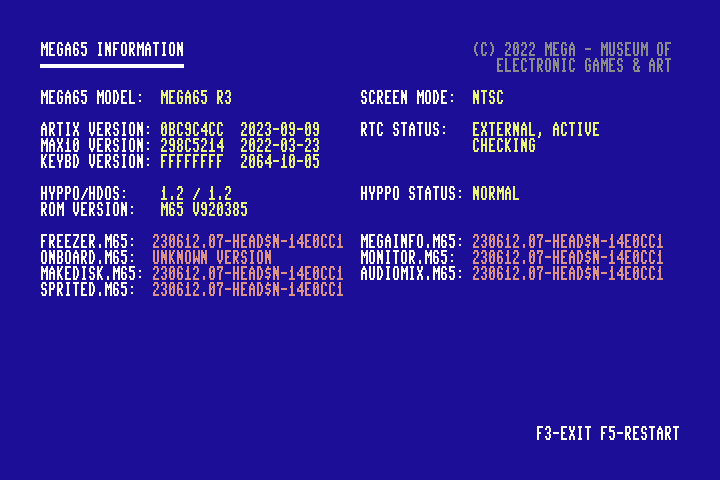
\includegraphics[width=0.7\linewidth]{images/megainfo.png}
\end{center}

Take note of these version identifiers:
\nopagebreak
\begin{center}
\setlength{\tabcolsep}{1mm}
\begin{tabularx}{\textwidth}{|X|p{7cm}|}
  \hline
  {\bf Label and Example} & {\bf Description} \\
  \hline
  MEGA65 Model\newline {\tt MEGA65 R5} & The revision of the hardware. You need to know this when downloading new core files. \\
  \hline
  Artix Version\index{Core!Version}\newline {\tt 93D55F08 2022-10-12} & The currently running MEGA65 core. This is a string of eight letters and numbers, and also a build date. \\
  \hline
  ROM Version\index{ROM!Version}\newline {\tt M65 V920377} & The currently running ROM. For MEGA65 ROMs, this is a sequential number, with larger numbers representing newer releases. \\
  \hline
  System files (.M65)\newline {\tt 221012.18-MASTER-5BBFDA9} & Each of the system software files has its own version identifier. Typically, you do not need to know these: you will upgrade these along with each core. The identifier is similar to the core version, but does not always match the currently running core. \\
  \hline
\end{tabularx}
\end{center}

Press \specialkey{F3} to exit to the Freezer, then \specialkey{F3} again to exit to BASIC.

Each core has a separate version for each hardware revision. As of the year 2023, the production models of the MEGA65 have used two different main board revisions, known as ``R3'' (more specifically ``R3A'') and ``R5.''\footnote{The MEGA65 ``DevKit'' model sold in the year 2020 is revision ``R3.'' It is also possible to run the MEGA65 core on certain FPGA development boards, with a separate version of the core file for each.}\index{Hardware revisions}

The MEGA65 core is available for all hardware revisions. If you are installing an alternate core and it is not available for your hardware revision, contact the author of the core.

\section{Obtaining the Latest Files}

You can download the latest MEGA65 core, ROM, and system software from the MEGA65 Filehost website.\index{Filehost website} Due to distribution restrictions for the Commodore 65 ROM code, some files require a Filehost account registered to a MEGA65 owner to access. All owners of the MEGA65 have a license to all versions of this ROM code.\footnote{There is a procedure for non-owners to get the latest MEGA65 ROM, such as to use with the \href{https://github.lgb.hu/xemu/}{Xemu MEGA65 emulator}. This involves downloading \href{https://www.c64forever.com/}{C64 Forever Free Express Edition} from Cloanto, extracting the original Commodore 65 prototype ROM file, then using a tool to apply a patch that you can download from Filehost. The full process is described in the following article: \url{https://files.mega65.org?ar=145591dd-deb6-4bd0-aa89-8e39cd021470}}

Visit the following URL in your web browser:

\url{https://files.mega65.org}

\begin{center}
  \fbox{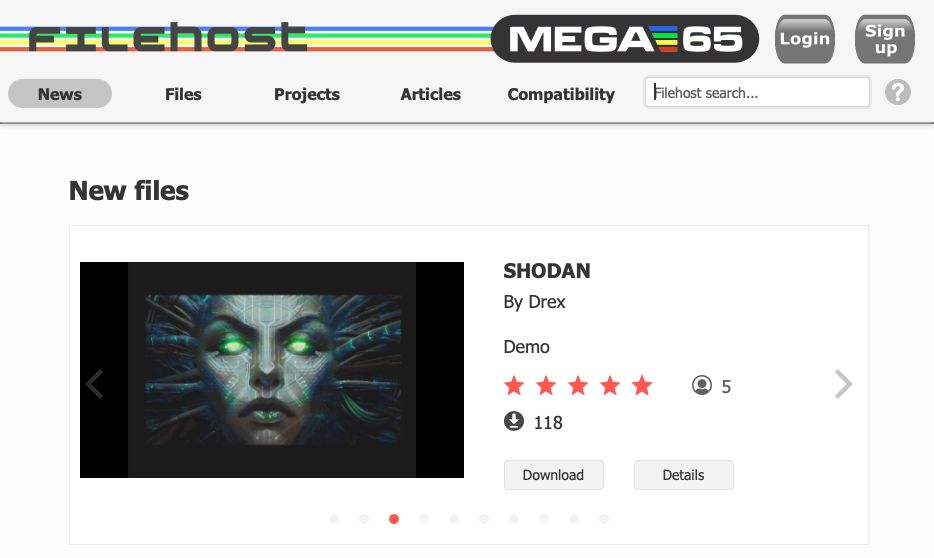
\includegraphics[width=0.7\linewidth]{images/filehost_notsignedin.png}}
\end{center}

To register a Filehost account with your owner code:

\begin{enumerate}
  \item Visit \href{https://files.mega65.org}{the Filehost website}. Click ``Sign Up.'' Follow the prompts to create an account.
  \item Locate your owner code.\index{Owner Code} This is a code printed on a piece of paper that was included with your MEGA65 (possibly inserted into this manual). It looks something like this: {\tt 123-ABC-456}
  \item Click the user icon in the upper-right corner of the Filehost screen. In the pop-up menu, select ``Redeem Code.'' Enter your owner code as prompted.
\end{enumerate}

\begin{center}
  \fbox{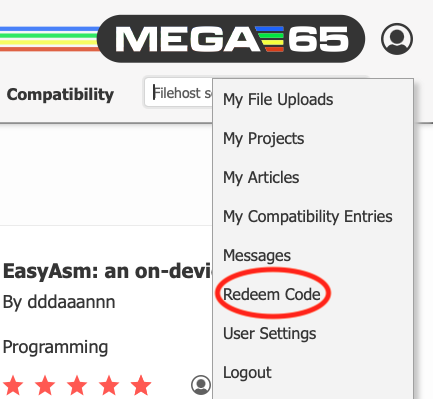
\includegraphics[width=0.4\linewidth]{images/filehost_redeemmenu.png}}
\end{center}

To download the latest release package:

\begin{enumerate}
  \item Click the ``Files'' tab of the Filehost website.
  \item In the search box on the left-hand side, type: ``release'' The list will update to show only files with that word in the title.
  \item Locate the entry named, ``MEGA65 Core Release Package (mega65r5) incl. ROM,'' where ``mega65r5'' matches your hardware revision. (To confirm your hardware revision, open the Freezer menu, then press \specialkey{Help}.)
  \item Click the entry. Confirm that this release package is for your hardware revision, then click ``Download'' to download the file.
\end{enumerate}

If you don't see an entry that says ``incl. ROM,'' check that you are signed in and that you have redeemed a valid owner code. Note that there is an entry for the Release Package that does not include the ROM that is visible to everyone. To ensure you are using a compatible set of files, get the package that says ``incl. ROM.''

\begin{center}
  \fbox{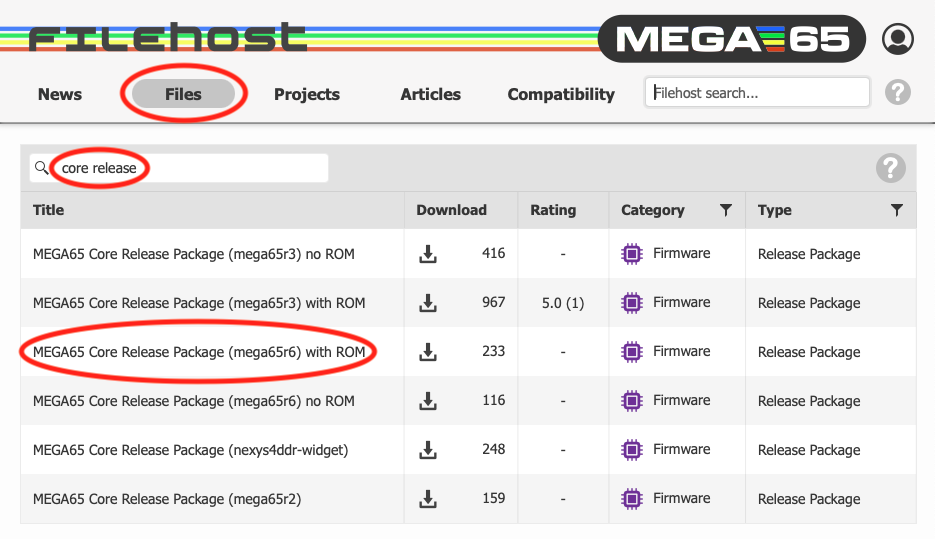
\includegraphics[width=0.7\linewidth]{images/filehost_release.png}}
\end{center}

Extract the downloaded {\tt .7z} archive. You should see a file whose name ends in {\tt .cor}, and a folder of {\tt sdcard-files} that includes one named {\tt MEGA65.ROM}.

\section{The Core Selection Menu}
\index{Core!Core Selection Menu}

The MEGA65 decides which core to load into the FPGA when it starts up. You can interrupt this process to select which core to load.\footnote{Technically, the MEGA65 starts the core in slot 0 to power the core selection menu. After you have made a selection or it chooses a default, it loads the selected core into the FPGA and continues the boot process.}

To open the core selection menu, switch off the computer, then hold the \specialkey{NO\\SCROLL} key and switch on the computer. The core selection menu appears, with the eight core slots numbered 0 through 7.

\begin{center}
  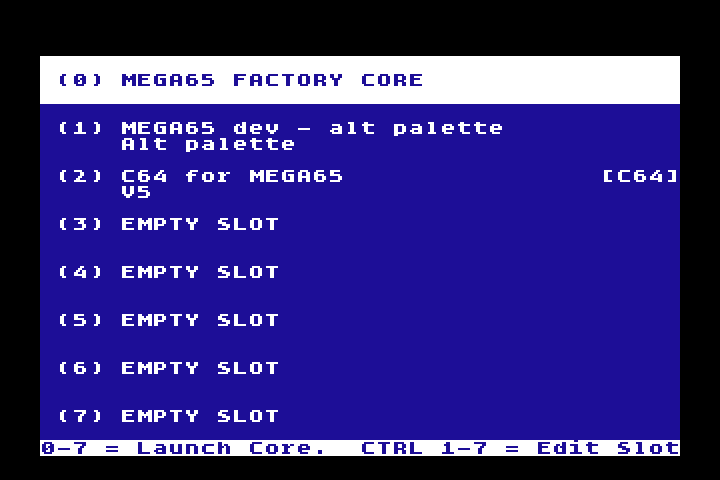
\includegraphics[width=0.7\linewidth]{images/ss-flashmenu.png}
\end{center}

You can select a core to boot using the cursor keys and \specialkey{RETURN}, or you can simply press the number key that corresponds to the slot. The boot process continues with the new core. The MEGA65 will keep running the new core until you physically power it off. (Pressing the reset button will not reset which core is being run.)

When you switch on the computer without opening the core selection menu, the MEGA65 looks for a core in slot 1. If there is a valid core in that slot, it uses it. Otherwise it tries slot 0.\footnote{You can change the default core slot from 1 to 2 by moving DIP switch \#4 to the ``on'' position. DIP switches are located inside the case, on the main board. For a diagram of the DIP switch locations, see \vref{cha:transferring-files}.}

Your computer comes with the MEGA65 core in slot 0 installed at the factory. It is recommended that you do not upgrade the factory-installed core under most circumstances. Instead, install new versions of the MEGA65 core in slot 1.

\section{Upgrading the MEGA65 Core, ROM, and System Files}
\index{Core!Upgrading}\index{ROM!Upgrading}

You can upgrade a core or install a new core from the core selection menu. This process reads the {\tt .cor} file from the SD card.

To upgrade the MEGA65 core, ROM, and system files:

\begin{enumerate}
  \item Remove the SD card (or microSD card) from the MEGA65, and connect it to your PC using an SD card reader.\footnote{As an alternative to moving the SD card to your PC, you can transfer files using an Ethernet connection. See chapter \vref{cha:transferring-files}.}
  \item Copy the {\tt .cor} file that you extracted from the {\tt .7z} archive to the SD card.
  \item On your PC, open the {\tt sdcard-files} folder from the {\tt .7z} archive, then copy those files to the SD card, replacing the existing files. Put them in the root of the SD card's file system, not a sub-folder.
  \item Eject the SD card from your PC's operating system, then move it back to the MEGA65.
  \item Open the core selection menu: Switch off the MEGA65, then hold \specialkey{NO\\SCROLL} while switching it back on.
  \item Hold \specialkey{CTRL} then press the number of the slot you want to upgrade. Follow the prompts. This process asks for a key press several times, and takes several minutes.
\end{enumerate}

When you start the update process, it prompts you to select the {\tt .cor} file on a screen that looks similar to this:

\begin{center}
  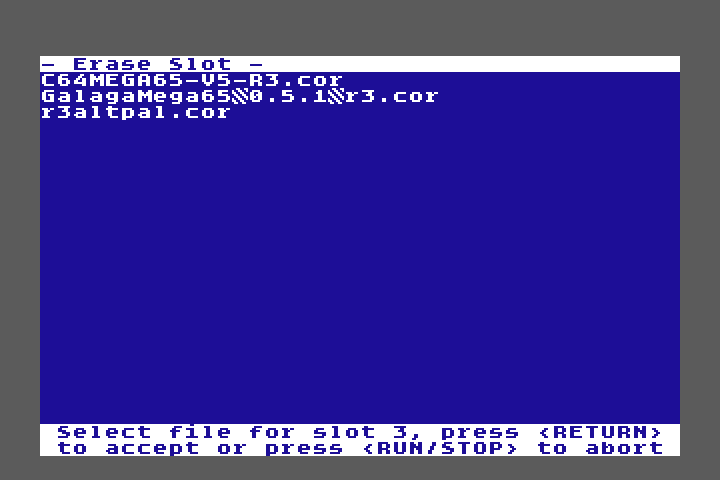
\includegraphics[width=0.7\linewidth]{images/ss-flashmenu-selectcore.png}
\end{center}

The process begins by checking that the core file matches your hardware revision. Press any key to continue.

\begin{center}
  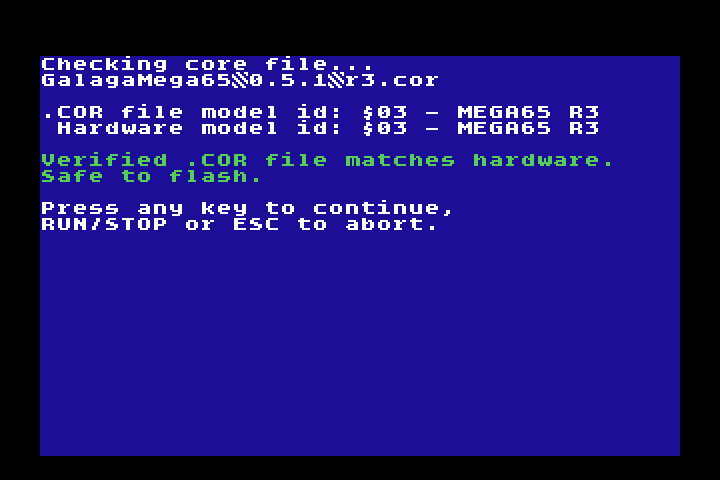
\includegraphics[width=0.7\linewidth]{images/ss-flashmenu-1-checking.png}
\end{center}

It then copies the file from the SD card to RAM, performing another check that the core file is complete.

\begin{center}
  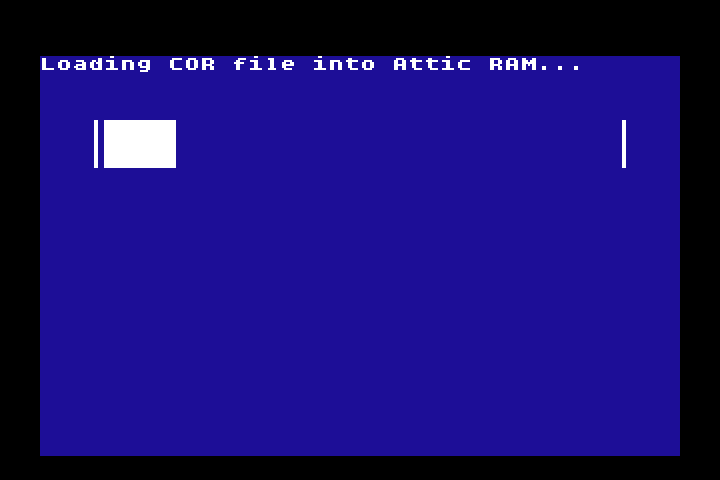
\includegraphics[width=0.7\linewidth]{images/ss-flashmenu-2-loading.png}
\end{center}

It presents the result of this check before proceeding. If the check is valid, you will see a message similar to the following. Press any key to continue.

\begin{center}
  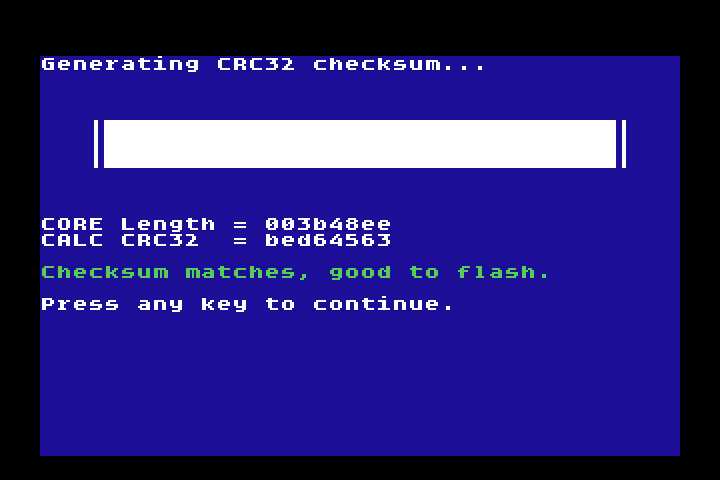
\includegraphics[width=0.7\linewidth]{images/ss-flashmenu-3-checksum-ok.png}
\end{center}

If the check is invalid, you will see the message, ``CHECKSUM MISMATCH.'' If you were not expecting this message, abort the process and confirm that you are using the correct file.\footnote{There are rare cases where a core may be valid but not have a correct checksum, such as if you are installing older versions of the core.}

Once you tell it to proceed, the MEGA65 begins programming the core data into flash memory. The border twinkles in coloured patterns during this process.

\underline{Note}: Do {\em not} switch off your computer or disconnect power until after this step is complete.

\begin{center}
  \fbox{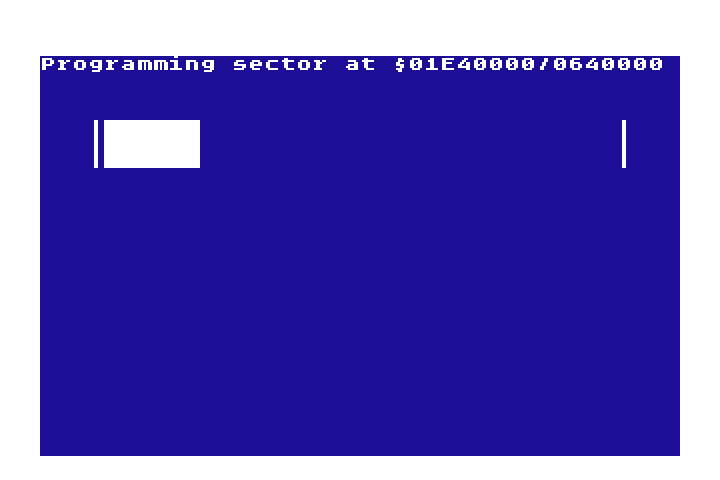
\includegraphics[width=0.7\linewidth]{images/ss-flashmenu-4-programming.png}}
\end{center}

When the process is complete, you will see a screen similar to the following.

\begin{center}
  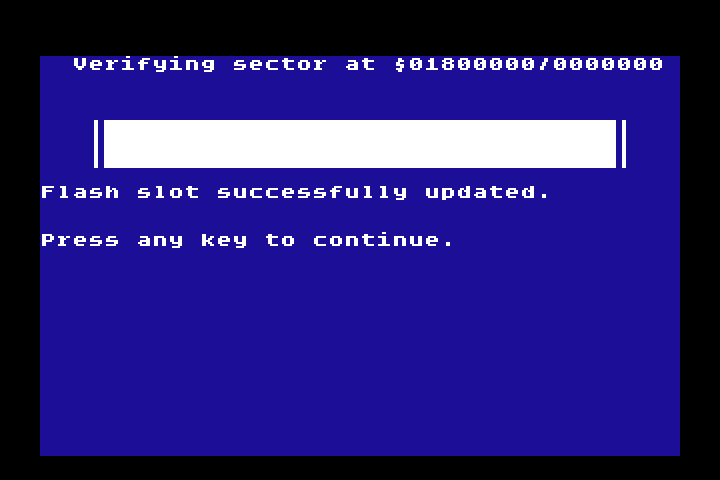
\includegraphics[width=0.7\linewidth]{images/ss-flashmenu-done.png}
\end{center}

It is now safe to switch off your computer. Press any key to return to the core selection menu, or switch the computer off then on again to start the default core.


\section{Installing Alternate Cores}

Installing an alternate core, such as the C64 core,\index{Core!C64 core} uses the same steps for flashing the core to a slot.

It is recommended to use slots 2 through 7 for alternate cores, and reserve slot 1 for the latest MEGA65 core. Of course, there is nothing stopping you from installing an alternate core in slot 1, so that the MEGA65 behaves as a different type of computer when you switch it on. You can always choose the MEGA65 core from the core selection menu.


% TODO: Document how to configure the boot core for cartridge types


\section{Upgrading the Factory Core in Slot 0}
\index{Core!Upgrading Slot 0}

It is possible to upgrade the factory-installed MEGA65 core in slot 0. You only need to do this in rare cases, such as if a newer version of the MEGA65 core includes changes or bug fixes for the start-up process. The process is elaborate, delicate, and could result in a MEGA65 that fails to start if something goes wrong. It is {\em strongly} recommended that you do not upgrade slot 0 unless the announcement for the release suggests that you do so. Most MEGA65 core upgrades are fully functional in slot 1, without needing to upgrade slot 0.

{\em Please read these instructions carefully before starting the procedure.}

\begin{enumerate}
  \item Prepare to use the {\em internal SD card only}. This may involve opening the case to make the SD card easier to access. Do {\em not} use the external microSD card slot for updating core slot 0.
  \item Using your PC, rename the core file that you wish to install to this exact filename: {\tt UPGRADE0.COR} (That's the word {\tt UPGRADE}, the number zero, and {\tt .COR}, using uppercase letters.)
  \item Install the latest MEGA65 core in slot 1, using the procedure described earlier. The core must be in the default non-zero slot to recover from any problems when updating slot 0. Boot this core to test that it works.
  \item Open the core selection menu. Press \megasymbolkey and the comma key to start the flash procedure for slot 0. (You will not be prompted for a filename.)
\end{enumerate}

\ifdefined\printmanual
\else
\underline{Note}: If you have a revision R3A MEGA65, have not previously upgraded slot 0, and \megasymbolkey and \megakey{,} does not start the procedure, you have an older slot 0 core that does not have this feature. You can work around this by restarting the core selection menu with slot 1. From the core selection menu, prepare to hold down \specialkey{NO\\SCROLL}, press the \megakey{1} key to boot into the core then immediately press and hold \specialkey{NO\\SCROLL}. The core selection menu re-opens using slot 1. Press \megasymbolkey and the comma key to complete the slot 0 upgrade.
\fi

If something goes wrong during the slot 0 flashing process, your MEGA65 may not start correctly. Before doing anything else, switch on your MEGA65, and wait a minute or so. It should notice that there is no valid core in slot 0, then proceed to start the core in slot 1. You can hold \specialkey{NO\\SCROLL} during this to open slot 1's core selection menu and restart the flashing process.

If the MEGA65 cannot boot any core after several minutes, it may be stuck. You may be able to recover using a device known as a ``JTAG interface'' that connects your PC to the MEGA65 main board. This allows you to inject a bitstream directly into the FPGA. The part is inexpensive but not always available. Contact the MEGA65 team on the Discord (\url{https://mega65.org/chat}) for assistance.


\section{Installing Alternate ROMs}

You can keep more than one version of the MEGA65 ROM on the SD card. When booting the MEGA65 core, you can select one of these ROMs by holding down a number key during boot.

To install alternate ROMs, copy them to the root of the SD card with a filename such as {\tt MEGA65x.ROM}, where {\tt x} is a number between 1 and 7. To boot the alternate ROM, hold the corresponding number key down while the MEGA65 core starts. If you do not hold down a number, it boots to {\tt MEGA65.ROM} by default.

There are several reasons you might want to keep alternate ROMs on your SD card:

\begin{itemize}
  \item You are helping to test a new beta release of the ROM, and do not wish to make the beta version your default ROM.
  \item You want to try the MEGA65 OpenROM, a project to create an all-new ROM released under an Open Source license without any original Commodore material.
  \item You want to try the original Commodore 65 prototype ROM. The MEGA65 core maintains backwards compatibility with the C65 ROM that was in progress by Commodore before they cancelled the project. It is buggy and incomplete, but is still an interesting historical artifact.
\end{itemize}

Several alternate ROMs came with your MEGA65 SD card, installed at the factory. Try rebooting your computer while holding down a number key to see what happens!


\section{Understanding The Core Booting Process}
\nopagebreak
This section summarises how the MEGA65 selects which core to start with when it is switched on. The process is shown in the following figure:
\nopagebreak
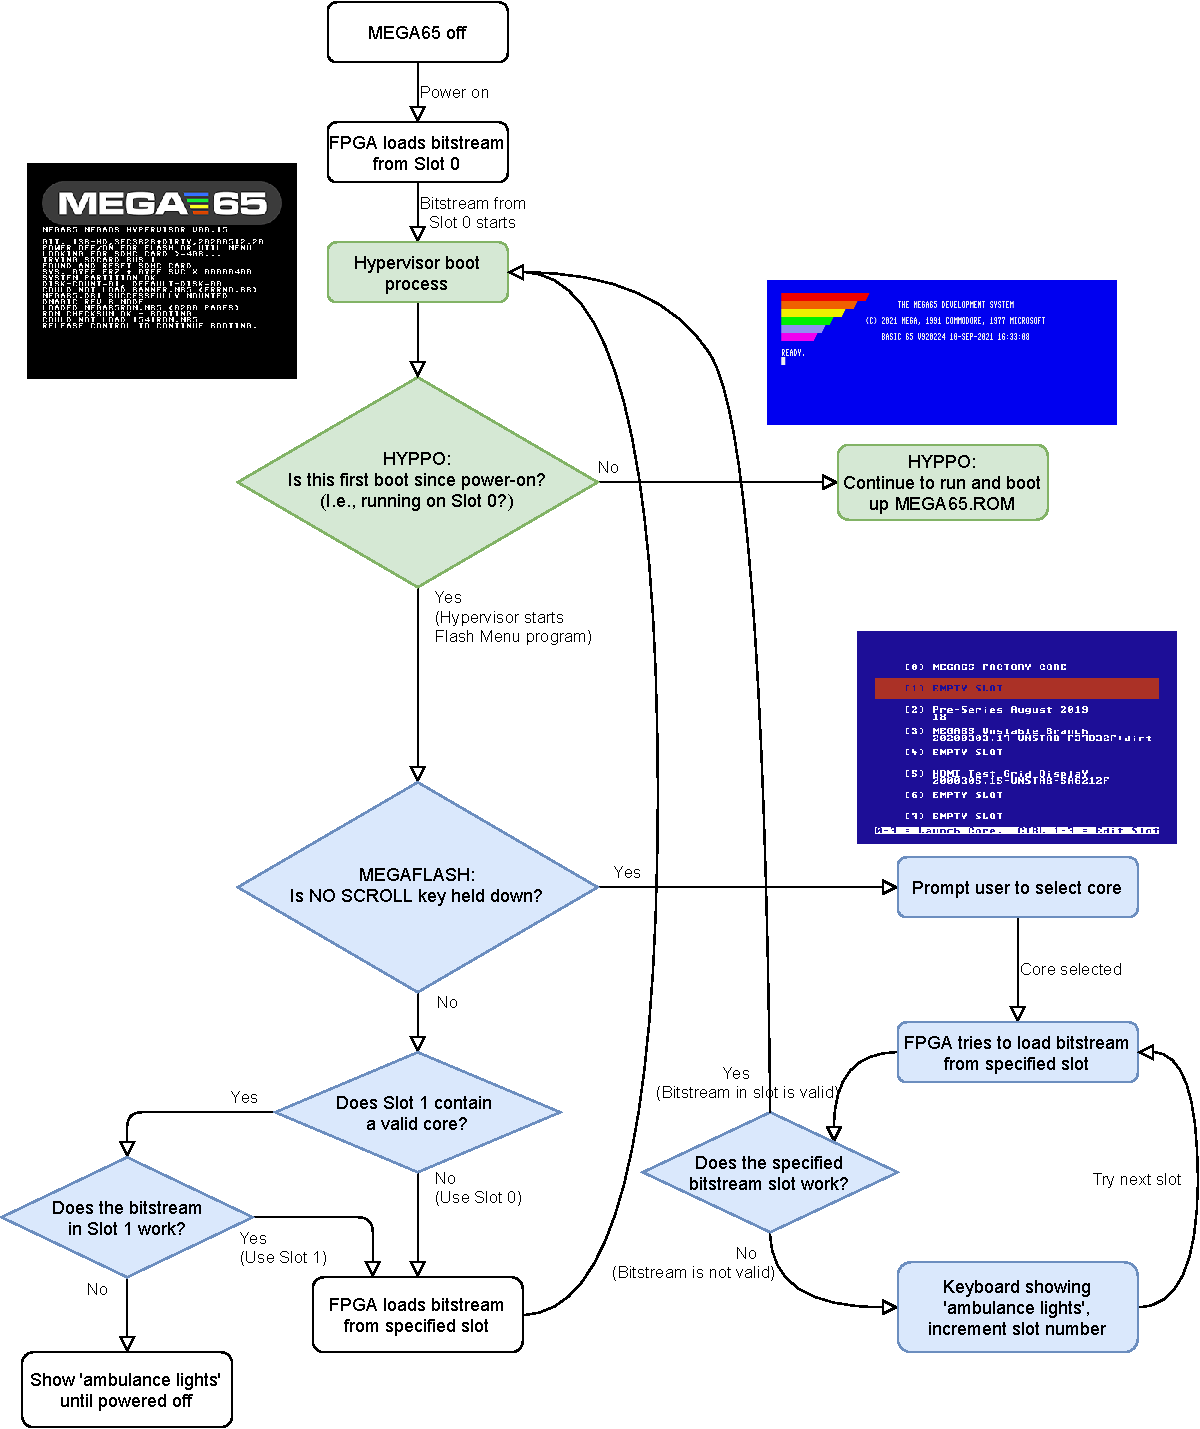
\includegraphics[width=\linewidth]{images/illustrations/flashmenu-flowchart.pdf}

The booting process is governed by two facilities:
\begin{itemize}
  \item The Hypervisor (also known as HYPPO), which operates at a level above the KERNAL. One of its responsibilities is to manage aspects of the boot process. For more details on the Hypervisor, refer to
\ifdefined\printmanual
the {\bf MEGA65 Book}.
\else
 \bookvref{sec:hypervisor-mode}.
\fi
    In the diagram, activities performed by the Hypervisor have been highlighted in green.
  \item The Core Selection Menu program (also known as ``MegaFlash''), which provides a list of available core slots to choose from. In the diagram, activities performed by MegaFlash have been highlighted in blue.
\end{itemize}

When the MEGA65 is switched on, it does the following:
\begin{itemize}
\item Loads the bitstream stored in slot 0 of flash memory. If that is the MEGA65 Factory Core, the MEGA65
  HYPPO Hypervisor starts.
\item If it is the first boot since power-on (which implies that you are running from slot 0), HYPPO starts the Flash Menu program (aka MegaFlash) -- but note that the Flash Menu in
      this mode may not show anything on the screen to indicate that it is running!
\item The Flash Menu then checks if \specialkey{NO\\SCROLL} is being held down.
\item If it is, the Flash Menu program shows its display, allowing you to select or re-flash a core.
\item If \specialkey{NO\\SCROLL} is {\em not} being held down, the Flash Menu program checks if Flash Slot 1 contains a valid
      core.
\item If it does, then the Flash Menu program attempts to load that core.
\item If it succeeds, then the system reconfigures itself for that core, after which the behaviour of the system is
      according to that core.
\item If it fails, the keyboard will go into ``ambulance mode'', showing flashing blue lights to indicate that some
      first-aid is required. Note that in ambulance mode the reset button has no effect: You must switch the
      MEGA65 off and on again.
\end{itemize}

If you have selected a different core in the Core Selection Menu, the process is similar, except that the ambulance lights will appear for only a limited time, as the FPGA will automatically search through the flash memory until it finds a valid core. If it gets to the end of the flash memory, it will start the MEGA65 Factory Core from slot 0 again.

\chapter{Using Disks and Disk Images}

\section{Disk Drives}
\label{cha:using-disks}
\index{Disk Drives}

The MEGA65 has a built-in 3.5" floppy disk drive, and supports Commodore-style external disk drives via the IEC serial port on the back of the computer. The IEC port also supports other external IEC storage devices, such as the SD2IEC.\index{SD2IEC device} Some IEC storage devices can be connected in a chain and used at the same time.

The MEGA65 also includes a ``virtual'' disk drive that can mount D81 or D64 disk image files\index{D81 disk image}\index{D64 disk image} stored on the SD card. Most MEGA65 software that you download from the Internet is in the form of a D81 disk image. Programs for the Commodore 64 are often distributed in the form of a D64 disk image. You can create a new D81 disk image directly from the MEGA65, and start saving your BASIC programs to the SD card without any additional hardware. You can also copy files between physical floppy disks and disk images.

The Intro Disk Menu\index{Intro Disk} that you saw when you first switched on the computer is a program on a D81 disk image, a file named {\tt MEGA65.D81} on the SD card. The MEGA65 is initially configured to boot this disk image automatically. You can change this in the Configuration Utility.\index{Configuration!Utility} (Refer back to chapter \vref{cha:configuringyourmega}.)

You can manage disk drives and virtual disk images from the Freezer menu.\index{Freezer menu} Some of these operations can be performed with BASIC commands such as {\bf MOUNT}.\index{BASIC 65 Commands!MOUNT}

\subsection{Unit Numbers and Drive Numbers}
\index{Disk Drives!Terminology}
\index{Connections!IEC}

Each disk drive (physical or virtual) is accessed via a {\it unit} number.\index{Unit number (IEC devices)} With vintage Commodore computers, the unit number refers to an IEC device connected to the computer. Commodore reserved unit numbers in the range 0 -- 31 for devices of various purposes, with 8 -- 11 reserved for disk drives. If you've ever used a Commodore 64 and typed \screentext{LOAD "*",8,1}, the ``8'' refers to the disk drive connected as unit 8. BASIC 65 disk commands use unit 8 by default, and accept a {\bf U} parameter to change it, such as: \screentext{DLOAD "MYPROGRAM",U9}\index{BASIC 65 Examples!DLOAD}\index{BASIC 65 Examples!LOAD}

With the MEGA65, you can assign a unit number to the virtual disk drive with a disk image mounted, or to the internal 3.5" floppy drive. You must mount a disk image or the internal 3.5" floppy drive to a unit number before it can be used. Any message sent to a unit number assigned to a virtual disk or the internal floppy drive is handled by the MEGA65. All other messages are sent to the IEC serial port.

Disk commands also accept an optional parameter to specify a {\it drive} number.\index{Drive number (IEC devices)} This is only needed when connecting a vintage dual floppy drive via the IEC port, such as the Commodore 4040, 8050, or 8250. Every disk drive assigns drive number 0 to the first drive. Dual-drive units assign a drive number of 1 to the second drive. Dual disk drives are usually equipped with an IEEE-488 interface, and need an IEEE-488 to IEC converter to be used on the MEGA65. BASIC 65 disk commands use drive 0 by default, and accept a {\bf D} parameter to change it.


\section{Using Virtual Disk Images}
\index{Disk Drives!D81 Images}

The MEGA65 provides two ``managed drives'' that supplement drives connected to the IEC port. The first managed drive can be assigned either a D81 or D64 disk image file on the SD card, or it can be assigned to the built-in 3.5" floppy drive. The second managed drive can also be assigned a D81 or D64 disk image file, for up to two virtual disks mounted at the same time.\footnote{Commodore originally intended to release a new external 3.5" floppy drive called the ``1565'' to go with the Commodore 65, connecting to a dedicated non-IEC port. The MEGA65 project has ambitions to someday produce such a drive, and if it does, this would be assigned to the second managed drive.}

The first managed drive can be set to unit 8 or 10, and the second managed drive can be set to unit 9 or 11.

\subsection{Where to Get Disk Image Files}

The MEGA65 Filehost website\index{Filehost website} hosts a library of MEGA65 software produced by the community. You can browse or search for software, download a title, then copy the disk image to the SD card using either your PC or the Ethernet file transfer tool.

\url{https://files.mega65.org/}

\subsection{Mounting Disk Images with the Freezer}

Open the Freezer menu:\index{Freezer menu} hold \widekey{RESTORE} for one second, then release it. Notice the current drive mounting settings in the lower-right of the screen.

\begin{center}
  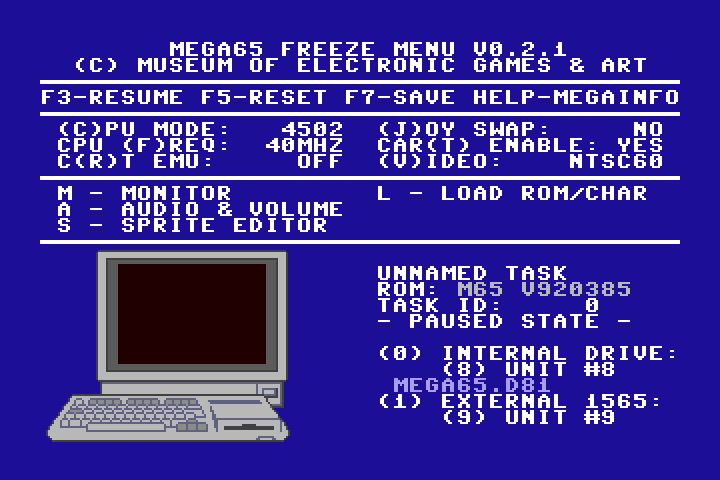
\includegraphics[width=0.7\linewidth]{images/freezer.png}
\end{center}

To mount a disk image on unit 8 or 10, select the first managed drive by pressing \megakey{0}. To mount a disk image on unit 9 or 11, select the second managed drive by pressing \megakey{1}. This opens the SD card file browser.

\begin{center}
  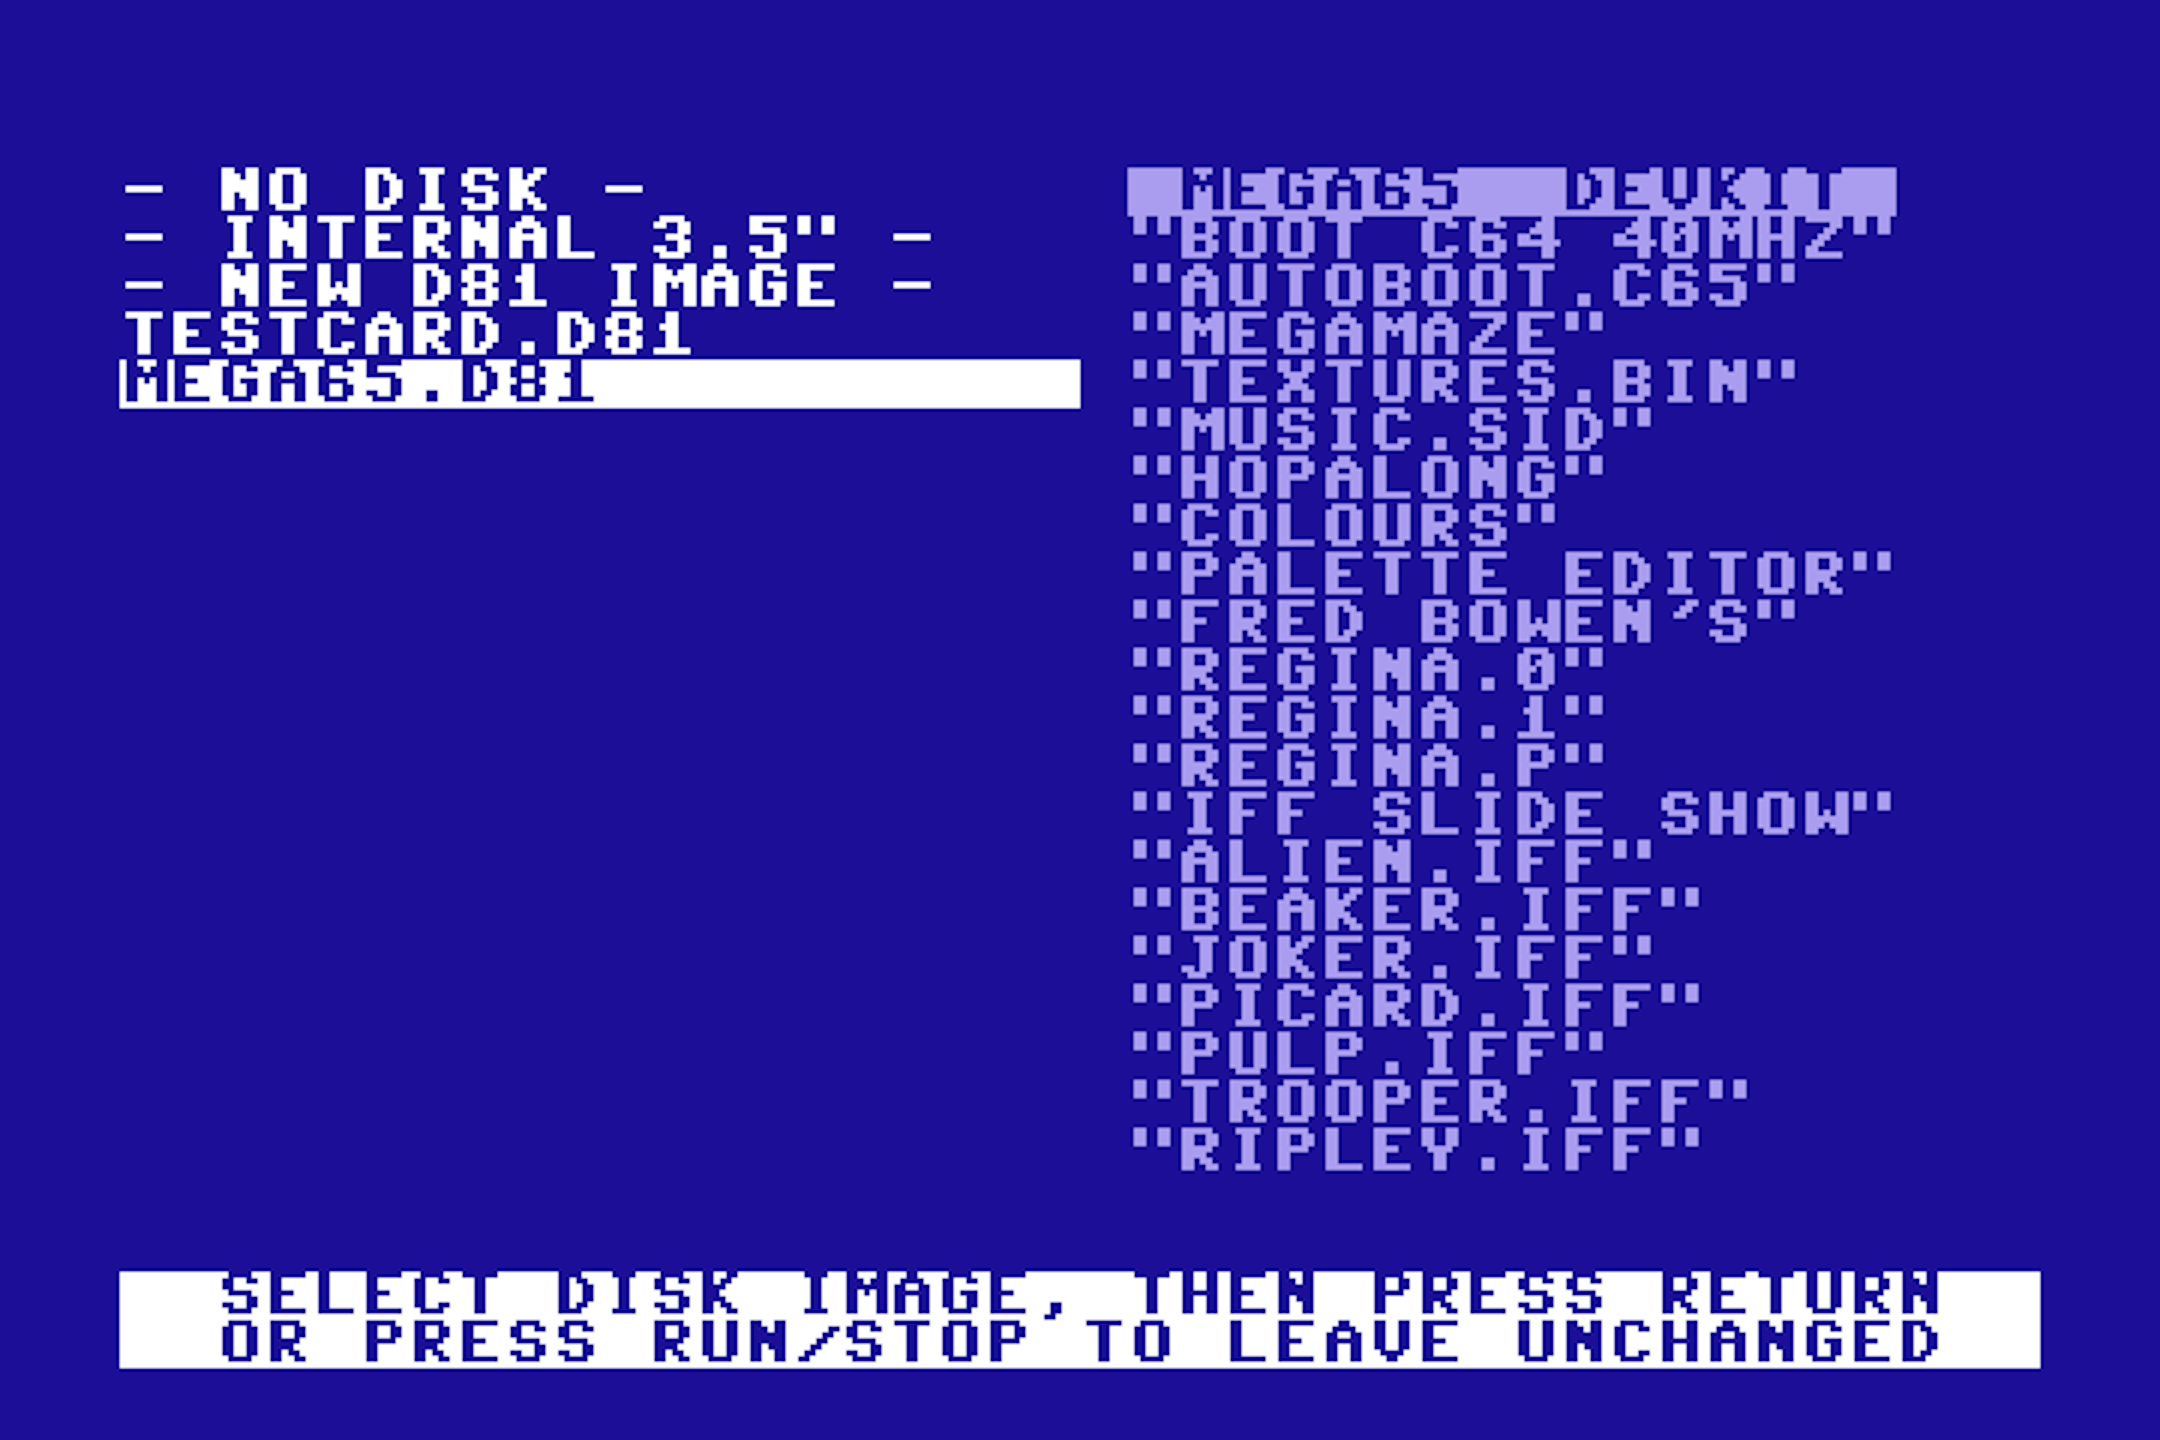
\includegraphics[width=0.7\linewidth]{images/d81-file-browser.png}
\end{center}

Use the cursor keys to select a disk image, then press \widekey{RETURN}. The Freezer screen shows the selected disk image is now associated with the managed drive.

From the main Freezer screen, press \megakey{8} or \megakey{9} to toggle the unit number assigned to the first or second managed drive, respectively.

\subsection{Mounting Disk Images from BASIC}

The BASIC {\bf MOUNT} command\index{BASIC 65 Commands!MOUNT} can mount a disk image from the SD card without having to open the Freezer. This command can be entered at the \screentext{READY} prompt, or be used as part of a program.

To mount a disk image on unit 8, enter {\bf MOUNT} with the full filename in double-quotes, including the {\tt .D81} or {\tt .D64} suffix:

\begin{screencode}
MOUNT "MEGA65.D81"
\end{screencode}

To mount a disk image to unit 9, provide the {\bf U} argument:

\begin{screencode}
MOUNT "MEGA65.D81",U9
\end{screencode}

\subsection{Creating a New Disk Image}
\index{Disk Drives!D81 Images}

You can create a new empty D81 disk image from within the MEGA65 Freezer.\index{Freezer menu}

\begin{enumerate}
\item Open the Freezer.
\item Press \megakey{0} to select the first managed drive.
\item At the top of the file list, select: \screentext{- NEW D81 DD IMAGE -}
\item When prompted, enter a name for the disk. (Omit the {\tt .D81} suffix; this will be added automatically.)
\end{enumerate}

The new disk image is created on the SD card and mounted to the first managed drive. It is formatted and ready to use.

\subsection{Managing SD Card Files in Sub-directories}

Once you have spent some time on Filehost downloading games and applications, you will eventually have a large collection of disk images on your SD card. You may wish to organize these files into sub-directories (folders). You can create these folders with the SD card connected to your PC, or with the Ethernet file transfer tool.

The Freezer supports sub-directories in its file browser. Each sub-directory name begins with a slash (\screentext{/}). Select a folder to list its files. To return to the previous folder, select: \screentext{/..}

You can also create new disk images in sub-directories by navigating to the sub-directory before selecting \screentext{- NEW D81 DD IMAGE -}.

The MEGA65 maintains a ``current working directory'' that is used as the base directory for BASIC commands such as {\bf MOUNT}. To change the current working directory from BASIC, use the {\bf CHDIR} command\index{BASIC 65 Commands!CHDIR} with the {\bf U12} argument:\index{BASIC 65 Examples!CHDIR}\index{BASIC 65 Examples!MOUNT}

\begin{screencode}
CHDIR "DEMOS",U12

MOUNT "XANADU.D81"
\end{screencode}

\underline{NOTE}: Support for sub-directories on the SD card is a work in progress. If a disk image in a sub-directory is mounted, it will become un-mounted by any action that changes the current working directory. Some features that use files may not support files in sub-directories. We hope to improve this in a future update.


\section{Using the Internal 3.5" Floppy Disk Drive}

The MEGA65 has a built-in 3.5" floppy disk drive, similar to what was intended for the Commodore 65. You can use physical floppy disks to store your programs and data. Some MEGA65 software can be purchased on floppy disk.

The internal 3.5" drive must be mounted before it can be used. It can be mounted to unit 8 or unit 10, in the first managed drive.

\subsection{Mounting the 3.5" Drive with the Freezer}

Open the Freezer menu:\index{Freezer menu} hold \widekey{RESTORE} for one second, then release it. Notice the current drive mounting settings in the lower-right of the screen.

Press \megakey{0}, then use the cursor down key to: \screentext{- INTERNAL 3.5" -} Press \widekey{RETURN} to select it. The Freezer menu screen shows that the internal drive is mounted to the first managed disk device.

The \screentext{UNIT \#} for the first device can be either 8 or 10. Press \megakey{8} to toggle between these options. BASIC disk commands default to unit 8, so it is typical to use unit 8 unless you are working with multiple disks at the same time.

The internal 3.5" drive can only be mounted in the first managed drive with unit numbers 8 or 10. It cannot be mounted in the second managed drive (unit numbers 9 or 11).

\subsection{Mounting the 3.5" Drive from BASIC}

You can mount the internal 3.5" disk drive to unit 8 using the BASIC {\bf MOUNT} command. This command works from either the \screentext{READY} prompt or from a program. To mount the internal drive to unit 8, enter the command without arguments:\index{BASIC 65 Examples!MOUNT}

\begin{screencode}
MOUNT
\end{screencode}

The {\bf MOUNT} command can only mount the internal drive to unit 8. You can only mount it to unit 10 from the Freezer menu.

\subsection{DD and HD disks}
\index{Disk Drives!Double-Density (DD) Disks}
\index{Disk Drives!High-Density (HD) Disks}

The MEGA65 disk controller expects a Double Density (DD) floppy disk in the internal 3.5" floppy disk drive.\footnote{It may be possible to support full-capacity HD disks in a future firmware update. The drive hardware is capable of reading HD disks.} Floppy disks are no longer manufactured, and the DD variety can be difficult to find.

You can use a High Density (HD) floppy disk with the drive, with one important modification: you must cover both sides of the hole in the upper-left corner (as seen from the front) of the disk with a small piece of tape. This convinces the drive that the disk is DD, and switches it to a mode compatible with the MEGA65 disk controller. A double-density disk does not have a hole in this location.

\begin{center}
  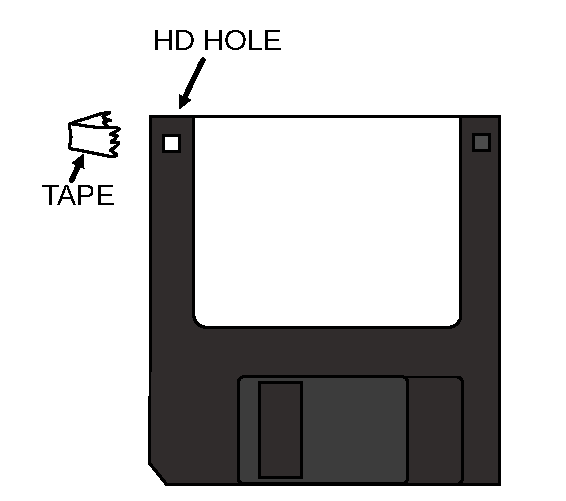
\includegraphics[width=0.75\textwidth]{images/illustrations/floppy_hd.pdf}
\end{center}

\underline{NOTE}: Make sure that the tape covers both sides of the hole.

\subsection{Formatting a Disk}
\index{Disk Drives!Formatting a Disk}

A floppy disk must be formatted before it can be used. The MEGA65's internal 3.5" floppy drive emulates a Commodore 1581 drive, and can use disks formatted in such a drive. You can also format a disk with the MEGA65.

\underline{NOTE}: Formatting a disk erases its contents. Be careful to only do this when you do not need the data on the disk!

To format a physical 3.5" floppy disk using the internal drive:

\begin{enumerate}
\item Open the Freezer.\index{Freezer menu}
\item Mount the internal 3.5" floppy drive to the first managed drive, unit 8.
\item {\it Double-check that unit 8 says:} \screentext{- INTERNAL 3.5" -}
\item Resume the computer: press \megakey{F3}.
\item Insert the floppy disk you wish to format into the internal floppy drive.
\item Enter the BASIC {\bf FORMAT} command, giving it a name ({\tt "MYDISK"}) and a two-character ID ({\tt XX}).\index{BASIC 65 Commands!FORMAT}\index{BASIC 65 Examples!FORMAT}
\begin{screencode}
FORMAT "MYDISK",IXX
\end{screencode}
\item When prompted, enter {\tt YES} and press \widekey{RETURN}.
\end{enumerate}

Formatting the disk takes a minute or so. The drive will make buzzing and clicking noises during the process. Do not switch off the computer or eject the disk until formatting is complete.

You can confirm that the formatting was successful by issuing the {\bf DIR} command.\index{BASIC 65 Commands!DIR} You should see an empty directory listing with the name and ID you specified. Your disk is now ready to use.


\section{Using External IEC Disk Drives}
\index{Connections!IEC}

The MEGA65 works with external disk drives connected to the IEC serial port.

External drives do not need to be mounted. If a unit number is not assigned to the internal 3.5" disk drive or to a disk image, disk operations intended for that unit number will be transmitted to the IEC serial port. It is up to the device connected to the port to recognize its unit number. Some IEC devices have switches that let you set the unit number. Others will only work with a specific number.

If you have an external drive that expects a specific unit number, you will need to make sure the MEGA65 isn't assigning that number to a disk image or the internal drive. Open the Freezer,\index{Freezer menu} then press \megakey{8} or \megakey{9} to toggle the unit number assignments so that they no longer use the needed unit number.\index{Unit number (IEC devices)}

The drive and unit assignments are temporary, and will be reset to their defaults when the MEGA65 is switched off. You will need to re-configure the drive assignments the next time you switch on the computer.


\section{Bootable Disks}
\index{Disk Drives!Bootable Disks}

With older Commodore computers, it was common for software makers to organize the file directory on a floppy disk such that the first file in the list is the main program. The user could then enter the command \screentext{LOAD "*",8,1} to load the main program, and \screentext{RUN} to run it. The asterisk is a wildcard that matches any file, so it matches the first file on the disk, without the user having to type the name of the program.

This method is still common, and the MEGA65 has a quick way to boot such disks: hold \specialkey{SHIFT} and press \specialkey{RUN\\STOP}. This executes the \screentext{RUN "*"} command, which is similar to the familiar command sequence that loads and runs the first program on the disk.\index{BASIC 65 Commands!RUN}

With the C65, Commodore introduced a new way to boot disks. Instead of relying on file order, a disk can have a file named {\tt AUTOBOOT.C65}.\index{AUTOBOOT.C65 file} If this file exists and is a program, the BASIC {\bf BOOT} command will load and run this file.\index{BASIC 65 Commands!BOOT}\index{BASIC 65 Examples!BOOT}

\begin{screencode}
BOOT
\end{screencode}

\subsection{Auto-Booting Disks}

As discussed in chapter \vref{cha:configuringyourmega}, you can use the Configuration Utility\index{Configuration!Utility} to set the MEGA65 to mount either a virtual disk image or the internal 3.5" disk drive automatically during boot.

If the mounted disk is bootable --- that is, it contains a program file named {\tt AUTOBOOT.C65} --- the MEGA65 will load and run the boot program automatically.

This is how the Intro Disk works. The Intro Disk menu is a program named {\tt AUTOBOOT.C65} on the virtual disk image {\tt MEGA65.D81}, which is pre-configured to be the mounted disk on system start-up. When you disable the Intro Disk from its menu, it renames {\tt AUTOBOOT.C65} to {\tt MENU}, such that the disk is no longer considered bootable.

Setting up a boot disk for yourself can be a handy way to configure your computer. You can write a short BASIC program that changes the system font, adjusts the background colour, and sets {\bf KEY} macros to your taste, then save the program as {\tt AUTOBOOT.C65} on a disk that you have configured to mount on system start-up. This program will run every time you switch on your MEGA65.


\section{Accessing the SD Card from BASIC}

Several BASIC 65 commands can operate directly on the MEGA65 SD card as if it were a disk drive. In these cases, the SD card is known as unit 12.

\underline{NOTE}: Unit 12 can only be accessed directly for a few specific operations. It cannot treat the entire SD card as if it were a CBDOS disk.

To list all of the files on the SD card, use the {\bf DIR} command with the \screentext{U12} argument:\index{BASIC 65 Commands!DIR}\index{BASIC 65 Examples!DIR}

\begin{screencode}
DIR U12
\end{screencode}

You can use the optional {\bf P} flag with this command to list the SD card files one page at a time. Press Q to stop at the current page, or any other key to advance to the next page.

\begin{screencode}
DIR U12,P
\end{screencode}

To load or save a PRG file directly from the SD card (that isn't in a disk image), use the \screentext{U12} argument with the {\bf DLOAD} and {\bf DSAVE} commands. You {\em must} include the {\tt .PRG} filename suffix in this case, which is different to using PRG files on disks or disk images.\index{BASIC 65 Commands!DLOAD}\index{BASIC 65 Commands!DSAVE}\index{BASIC 65 Examples!DLOAD}

\begin{screencode}
DLOAD "MYPROGRAM.PRG",U12
\end{screencode}

As shown earlier, the MEGA65 supports sub-directories (sub-folders) on the SD card, and maintains a current working directory for disk operations. To change the current working directory to a subdirectory:\index{BASIC 65 Commands!CHDIR}\index{BASIC 65 Examples!CHDIR}

\begin{screencode}
CHDIR "SUBDIR",U12
\end{screencode}

To change the current working directory to the parent of the current directory:

\begin{screencode}
CHDIR "..",U12
\end{screencode}

The {\bf MOUNT} command can mount a D81 or D64 disk image to a unit number. Even though this command refers to a file on the SD card, it does not use the \screentext{U12} argument. Instead, it uses the {\bf U} argument to set the unit number for the disk being mounted. The {\bf MOUNT} command uses the current working directory set by {\bf CHDIR} to locate the file.


\section{Common Disk Operations}

The following are some examples of common disk operations you can perform at the \screentext{READY} prompt. See the BASIC command reference in appendix \vref{cha:basic-reference} for more information.

Most commands that accept filenames also accept a {\bf U} argument that says which unit has the file. The default unit is 8.\footnote{The default disk unit for BASIC commands is 8 when the computer first starts. You can change it with the {\bf SET DEF} command.\index{BASIC 65 Commands!SET}}

\subsection{DIR}
\index{BASIC 65 Commands!DIR}\index{BASIC 65 Examples!DIR}

To display the directory (list of files) for a disk, use the {\bf DIR} command.

\begin{screencode}
DIR

DIR U9
\end{screencode}

Unlike the Commodore 64 method of loading the disk directory into BASIC memory, the {\bf DIR} command does not modify BASIC memory. It is safe to use {\bf DIR} with a program in memory.

To make larger directories easier to view, {\bf DIR W} (for ``wide'') displays the directory in columns, pausing for each page.

\subsection{DLOAD and RUN}
\index{BASIC 65 Commands!DLOAD}\index{BASIC 65 Examples!DLOAD}
\index{BASIC 65 Commands!RUN}\index{BASIC 65 Examples!RUN}

The {\bf DLOAD} command loads a program from disk into memory. The {\bf RUN} command runs the program currently in memory.

\begin{screencode}
DLOAD "COOLGAME"
RUN
\end{screencode}

You can combine these into one command by providing the filename directly to the {\bf RUN} command.

\begin{screencode}
RUN "COOLGAME"
\end{screencode}

\subsection{DSAVE}
\index{BASIC 65 Commands!DSAVE}\index{BASIC 65 Examples!DSAVE}

The {\bf DSAVE} command saves the BASIC program currently in memory to disk.

\begin{screencode}
DSAVE "MYGAME"
\end{screencode}

By default, this will not overwrite an existing file with the same name. To request that the existing file be overwritten, insert an {\tt @} (at) symbol before the filename, inside the double-quotes.

\begin{screencode}
DSAVE "@MYGAME"
\end{screencode}

Note that save-with-replace is only recommended when using disk images and the 3.5" floppy drive. Older Commodore drives have bugs in this feature that could result in data loss.

\subsection{BACKUP}
\index{BASIC 65 Commands!BACKUP}\index{BASIC 65 Examples!BACKUP}

The {\bf BACKUP} command copies an entire disk from one unit to another. All existing data on the destination disk is erased as part of this process.

\begin{screencode}
BACKUP U8 TO U9
\end{screencode}

You can use {\bf BACKUP} to make disk images from floppy disks, or write disk images to floppy disks, or copy everything from one disk drive to another.

\subsection{COPY}
\index{BASIC 65 Commands!COPY}\index{BASIC 65 Examples!COPY}

The {\bf COPY} command makes a copy of a file. If the source and the destination are different filenames on the same unit, this duplicates the file on the disk.

\begin{screencode}
COPY "MYGAME", U8 TO "MYGAME", U9

COPY "MYGAME" TO "MYGAME-V1"
\end{screencode}

\subsection{RENAME}
\index{BASIC 65 Commands!RENAME}\index{BASIC 65 Examples!RENAME}

The {\bf RENAME} command changes the name of an existing file.

\begin{screencode}
RENAME "MYGAME-V29" TO "MYGAME-FINAL"
\end{screencode}

\subsection{DELETE}
\index{BASIC 65 Commands!DELETE}\index{BASIC 65 Examples!DELETE}

The {\bf DELETE} command deletes a file.

\begin{screencode}
DELETE "JUNKFILE"
\end{screencode}


\subsection{Shortcut Disk Commands}

BASIC 65 provides several shortcuts for common disk commands for use from the \screentext{READY} prompt. Remember though, shortcuts are run on the currently set default unit.

\begin{center}
\begin{tabular}{|l|l|}
\hline
{\bf Shortcut} & {\bf Equivalent Command} \\
\hline
\screentextwide{/} & {\bf LOAD} \\
\hline
$\uparrow$ & {\bf RUN} \\
\hline
$\leftarrow$ & {\bf SAVE} \\
\hline
\screentextwide{@} & {\bf DISK} \\
\hline
\screentextwide{\$} & {\bf DIR} \\
\hline
\end{tabular}
\end{center}

These are intended to be used with a directory listing to launch programs without having to type filenames. For example:

\begin{enumerate}
\item Display the disk's directory listing: type {\bf \$}, press \widekey{RETURN}.
\item Use the cursor keys to move the cursor to the line with the program you want to run.
\item Type {\bf \screentext{$\uparrow$}}, press \widekey{RETURN}.
\end{enumerate}

The selected program loads and runs. Notice that you do not have to clear extra characters from the line. The shortcut knows to ignore everything but the filename in double-quotes, as printed by the directory listing.

\chapter{Transferring Files}

\section{Transferring Files}
\label{cha:transferring-files}
\index{SD Cards!Transferring Files}

While there is plenty of fun to be had writing your own programs for the MEGA65, eventually you will want to run programs written by others. You may also want to back up your MEGA65 programs to your PC for safe keeping.

You can copy D81 virtual disk images to your MEGA65-formatted SD card using any PC, without any special tools or software. Your PC will recognize the data region of the SD card as a FAT32 partition. If you use this method, be aware that some PC operating systems may have unwanted side effects, such as fragmentation of SD card files, or extraneous files created by macOS Finder. These effects are harmless to the data, but may require maintenance to keep the card useful in the MEGA65.\footnote{If the MEGA65 reports a fragmented file, you can use a PC disk defragmentation tool on the data partition. Alternatively, you can copy all files off of the SD card to the PC, re-format the SD card in the MEGA65, then copy the files back from the PC.}

The fastest and most reliable way to transfer files between your PC and your MEGA65 is with an Ethernet cable.\index{Networking!Ethernet} You connect one end of the cable to the RJ45 jack on the rear of the MEGA65. You can connect the other end to your local area network (LAN) router or switch, or connect it directly to your PC. You use software on your PC to initiate file transfers, in either direction: from the PC to the MEGA65, or from the MEGA65 to the PC.

It is also possible to transfer files using a JTAG or UART Serial interface connected to the main board. This is an advanced technique and is not described in this User's Guide. Most people will prefer the Ethernet method.\footnote{JTAG or UART Serial hardware provides access to a debugging interface that may be useful to some programmers. JTAG is also useful for developing FPGA cores. For more information, see {\it MEGA65 Developer's Guide.}}

\section{Understanding Networking}

The MEGA65 can use Ethernet to connect to or accept connections from other computers on a network. With appropriate software, it can connect to other computers over the Internet.

The MEGA65 Ethernet hardware presents a Media Access Control (MAC) address to the local network.\index{Networking!MAC address} Unlike other Ethernet hardware, the MEGA65's MAC address is not assigned at the factory: it is set in the Configuration Utility. (See chapter \vref{cha:configuringyourmega}.)

% TODO: IP address handling may change before v0.96 is released. The new version will allow the PC to set the IP address of the MEGA65 for the session, and may or may not involve DHCP. It may also detect broadcast addresses automatically. Change pending as of September 6, 2023.

For file transfers, you instruct the MEGA65 to listen for incoming connections, then use M65Connect on your PC to initiate a connection. The MEGA65 always listens on IP address {\bf x.x.x.65} of your local subnet. You will need to know your local network's {\em broadcast address} to establish the connection. A typical home router establishes a local network with a broadcast address such as \texttt{192.168.0.255}. With this broadcast address, the local IP address of the MEGA65 would be \texttt{192.168.0.65}.

Modern computers typically use the Dynamic Host Configuration Protocol (DHCP) to obtain an IP address from the local router. The MEGA65 network listener does not support DHCP, and always listens on address 65. You will need to configure your router to prevent the address 65 from being assigned to another computer. See your router's documentation for information on how to do this. (It is possible to avoid this step if no other computer on your network is assigned address 65, but it's best to not leave this to chance.)

Most local network routers are configured to block incoming connections originating from the Internet (a ``firewall''). This is an important safety precaution in general. This is especially important for the MEGA65, because the MEGA65 network listener has no security protections of its own. {\em Do not configure your network router to allow incoming connections to reach the MEGA65 when using the network listener feature described below.}

As an alternative to connecting the MEGA65 to your local network, if your PC has an Ethernet jack, you can connect your MEGA65 directly to your PC via Ethernet.

\section{Obtaining the File Transfer Tools}
\index{M65Connect Application}

{\bf M65Connect} is an application for Windows, Mac, or Linux that facilitates file transfers and other useful features for MEGA65 users. The application has a windowed interface, and also includes command-line tools useful for programming.

To obtain M65Connect:

\begin{enumerate}
\item Visit the MEGA65 Filehost website\index{Filehost website} in a browser: \url{https://files.mega65.org}
\item In the search box in the top right corner, type: ``M65Connect''
\item Select the version of M65Connect for your PC operating system.
\item Click the ``Download'' button.
\item Use your PC to unpack the downloaded archive file.
\end{enumerate}

\subsection{M65Connect for Windows}

The Windows version of M65Connect is in the ``M65Connect'' folder: {\bf M65Connect.exe}. As with most open source software, Microsoft Defender may refuse to run the software, displaying a dialog window. If this happens, click ``More info,'' then click the ``Run anyway'' button that appears.

The command-line tools are in a sub-folder named ``M65Connect Resources,'' such as: {\tt M65Connect Resources/mega65\_ftp.exe}

\subsection{M65Connect for macOS}

The macOS version of M65Connect is a Mac application bundle: {\bf M65Connect.app}. As with most open source software, macOS does not recognize it as ``signed'' by the developer, and macOS will refuse to run it. To run the application for the first time:

\begin{enumerate}
\item Right-click on the {\bf M65Connect.app} icon. In the pop-up menu, select ``Open.'' A dialog will open.
\item Click the ``Open'' button. The application will open.
\end{enumerate}

On subsequent runs, you can double-click the icon as with any other application.

The command-line tools are inside the application bundle directory, such as: {\tt M65Connect.app/Contents/mega65\_ftp.osx}

\subsection{M65Connect for Linux}

The Linux version of M65Connect is in the ``M65Connect'' folder: {\bf M65Connect}. Double-click it to run.

The command-line tools are in a sub-folder named ``M65Connect Resources,'' such as: {\tt M65Connect Resources\\mega65\_ftp}

\section{Enabling Network Listening}
\index{Networking!Network Listening Mode}

By default, the MEGA65 ignores all attempts by other computers to connect to it over the network. Software running on the MEGA65 can listen for network connections, but the MEGA65 does not do this on its own.

To transfer files with M65Connect, you must set the MEGA65 to listen for incoming connection attempts from M65Connect. This requires two steps:

\begin{itemize}
\item Set the DIP switch \#2 on the main board to the ``on'' position.
\item Enable a network listening session by pressing this key combination: \specialkey{SHIFT} + \megakey{\pounds}
\end{itemize}

To set the DIP switch,\index{DIP switches} open the case, as described in \vref{cha:setup}. Locate the DIP switches on the main board, then set DIP switch \#2 to the ``on'' position.

\begin{center}
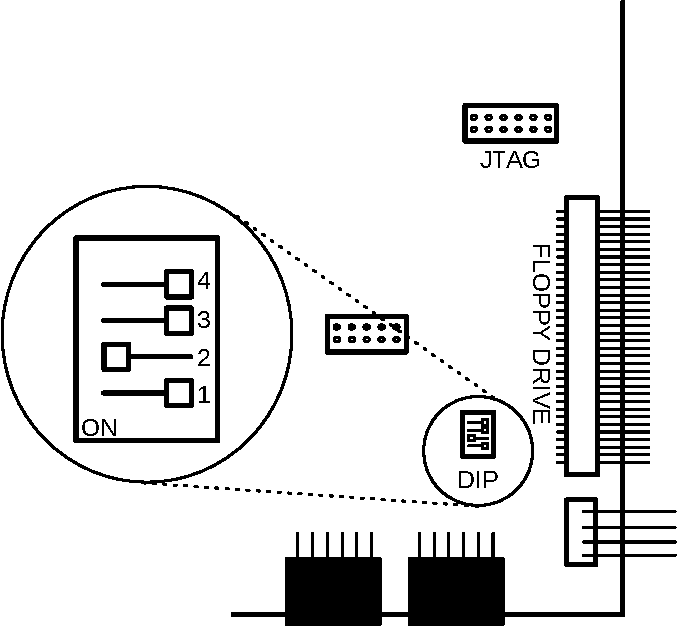
\includegraphics[width=\linewidth]{images/illustrations/mega65-dip2.pdf}
\end{center}

It is safe to leave DIP \#2 in this position for regular operation. It is set to off at the factory to avoid accidental activation.

To enable a network listening session, press \specialkey{SHIFT} + \megakey{\pounds}. The power light blinks between yellow and green when network listening is active.

\begin{center}
\includegraphics[width=\linewidth]{images/illustrations/mega65-eth-blink.pdf}
\end{center}

\underline{Note}: Resetting the computer disables network listening. Press \specialkey{SHIFT} + \megakey{\pounds} to start a new session.

\section{Transferring Files}

To transfer files, you will start a file transfer session using the M65Connect application or the {\tt mega65\_ftp} command-line tool. This connects to the MEGA65 and uploads a file transfer client for use during the session. When you end the session, the MEGA65 resets.

Starting a file transfer session resets the MEGA65. As a precaution, the session will not start if there is a program in memory. Save any programs or data, then clear program memory (such as with the {\bf NEW} command) before proceeding.

\underline{Note}: If you clear memory by resetting the computer, remember to re-enable network listening: press \specialkey{SHIFT} + \megakey{\pounds}, and ensure the power light is blinking.

\subsection{Transferring Files with M65Connect}
\index{M65Connect Application}

(This section is pending the release of a new version of M65Connect.)

% TODO: These instructions are pending an update to M65Connect that implements this procedure.

\subsection{The mega65\_ftp Command-Line Tool}
\index{mega65\_ftp command@\texttt{mega65\_ftp command}}

The {\tt mega65\_ftp} command-line tool initiates a file transfer session with the MEGA65. It can run interactively in the terminal and accept multiple file transfer commands, or it can run non-interactively with those commands provided as arguments.

% TODO: IP address handling may change before v0.96 is released. The new version will not require a broadcast address on the command line. Change pending as of September 6, 2023.

To start an interactive file transfer session, run the {\tt mega65\_ftp} command, providing the broadcast address as the {\tt -i} argument.

\begin{verbatim}
% mega65_ftp -i 192.168.0.255
\end{verbatim}

The tool will upload the file transfer client, and you will see it the client running on the MEGA65. If nothing happens, press Ctrl-C (on the PC) to abort, then double-check that the MEGA65 is connected and that network listening is enabled.

Once connected, the file transfer command prompt looks similar to this:

\begin{verbatim}
MEGA65 SD-Card:/>
\end{verbatim}

To end the session, use the {\tt exit} command. The tool will exit and return to the shell prompt, and the MEGA65 will reset.

\begin{verbatim}
MEGA65 SD-Card:/> exit
%
\end{verbatim}

The following are several useful commands you can use during the file transfer session. Use the {\tt help} command to see a complete list of available commands.

\begin{center}
\begin{tabular}{|l|l|}
\hline
{\bf Command} & {\bf Description} \\
\hline
{\tt put {\it filename}} & Send a file from the PC to the MEGA65. \\
\hline
{\tt get {\it filename}} & Retrieve a file from the MEGA65 to the PC. \\
\hline
{\tt dir} & Display a directory listing of the MEGA65 SD card. \\
\hline
{\tt ldir} & Display a directory listing of the local current working directory. \\
\hline
{\tt mkdir {\it dirname}} & Create a sub-directory on the MEGA65 SD card. \\
\hline
{\tt cd {\it dirname}} & Change the current working directory on the MEGA65 SD card. \\
\hline
{\tt help} & Display a list of available commands. \\
\hline
{\tt exit} & End the file transfer session. \\
\hline
\end{tabular}
\end{center}

To invoke {\tt mega65\_ftp} commands without starting an interactive prompt, use the {\tt -c} argument once for each command:

\begin{verbatim}
% mega65_ftp -i 192.168.0.255 -c 'put mydisk.d81' -c 'exit'
\end{verbatim}

The tool will start a session, execute the commands, then terminate. Be sure to issue the {\tt exit} command as the final command to reset the MEGA65, or reset the MEGA65 manually after the file transfer has completed.

\part{FIRST STEPS IN CODING}

\chapter{How Computers Work}

Did you know that many computer experts and programmers learned how to
use computers when they were still small children?
Home computers only became common in the early 1980s. They were so new,
that people would often write programs to do
what they wanted to do, because no software existed to do the job for them.

It was also quite common for people working in all
sorts of office jobs to learn how to program the computers they used for
their jobs.  For example, the people processing payroll
for a company would often learn how to program the computer to calculate
everyone's pay!

Things have changed a lot since then, though.
Now most people choose existing programs or apps to do what they need,
and think that programming is a specialised skill that only some people
have the ability to learn.
But this isn't true.  Of course, like every other field of pursuit
everyone will be better at some things than others,
whether it be sports, knitting, maths or writing. But almost
everyone is able to learn enough to help them in their life.

We created the MEGA65, because we believe that YOU can learn to
program, so that computers can be more useful to you, and as with
learning any new skill, that you can have the satisfaction, enjoyment,
and new adventures that this brings!


\phantomsection
\section{Computers are stupid. Really stupid}

How can this be so? Computers are able to do so many different things, often thousands of times faster than a person can.
So how can we say that computers are stupid?  The answer is that no computer can do anything that it hasn't been instructed
by a person to do.  Even the latest Artificial Intelligence systems were instructed how to learn (or how to learn, how to learn).
To understand why this is so, it is helpful to understand how computers really work.

\subsection{Making an Egg Cup Computer}

The heart of a computer is its Central Processing Unit, or CPU for short.  Many modern computers have more than one CPU, but let's keep
things simple to begin with.  The CPU has a set of simple instructions that it understands, like, ``get the thing from cup \#21,'' ``put this thing into cup \#403,'' ``add these things together,'' or ``do the following instruction, but only if the thing in cup \#712 is the number 3.''

But what do we mean with all of these ``things'' and ``cups''? Let's start by thinking about how we could pretend to be a computer using
just an empty egg carton, some small pieces of paper and a pencil or pen.  Start by writing numbers, beginning with one, in each of the
little egg cups in the egg carton.  Then write the number zero on a little scrap of paper and put it in the first cup.  Do the same for the other cups. You should now have an egg carton with numbered cups, and with every cup having a scrap of paper with the number zero written on it. Now we just need to decide on a few simple rules that will explain how our egg-cup computer will work:

\begin{itemize}
  \item First, each cup is allowed to hold exactly one thing at a time. Never more. Never less.  This is so that when we ask the question ``what is in box such-and-such,'' that there is a single clear answer. It's also how computer memory works: Each piece of memory can hold only one thing at a time.

  \item Second, we need a way for the computer to know what to do next. On most computers this is called the Program Counter, or PC, for short (not to be confused with PC when people are talking about a Personal Computer).  The PC is just the number of the next memory location (or in our case, egg-cup), that the computer will examine, when deciding what to do next.  You might like to have another piece of paper that you can use to write the PC number on as you go along.

  \item Third, we need to have a list of things that the egg-cup computer will do, based on what number is in the egg-cup indicated by the 
    PC.
\end{itemize}

So let's come up with the set of things that the computer can do, based on the number in the egg-cup indicated by the PC.  We'll keep things simple with just the following:

\begin{center}
  \begin{longtable}{|R{2.2cm}|p{8cm}|}

    \hline
        {\textbf{Number in the egg-cup}} & {\textbf{Action}} \\ \hhline{|=|=|}
        0 & {i) Add one to the PC, and do nothing else.} \\ \hline
        1 & {i) Add one to the PC. \hfill\break ii) Set the PC to be the number stored in that egg-cup.} \\ \hline
        2 & {i) Add one to the PC. \hfill\break ii) Add the number in the egg-cup indicated by the PC to the number in the egg-cup indicated by the number in the egg-cup following that. \hfill\break iii) Put the answer in the egg-cup indicated by the egg-cup following that. \hfill\break iv) Finally, add two more to the PC, to skip over the egg-cups that we made use of.}  \\ \hline
  \end{longtable}
\end{center}

Don't worry if that sounds a bit confusing for now, especially that last one -- we will go through it in detail very soon!
The best way to explain it is to go through some examples.


\chapter{Getting Started in BASIC}
\label{cha:basic-getting-started}

It is possible to code on the MEGA65 in many languages,
however most people start with BASIC.  That makes sense,
because BASIC stands for Beginner's All-purpose Symbolic
Instruction Code: It was made for people like you to get
started with in the world of coding!

A few short words before we dive in: BASIC is a programming
language, and like spoken language it has conventions, grammar
and vocabulary.  Fortunately, it is much quicker and easier
to learn than our complex human languages. But if you pay
attention, you might notice some of these structures, and that
can help you along your path in the world of coding.

If you haven't already read \bookvref{cha:getting-started},
it might be a good idea to do so. This will help you be able to
more confidently interact with the MEGA65 computer.

It's also great to remember that if you really confuse the MEGA65,
you can always get back to the READY. prompt by just pressing the
reset button on the left-hand side of the keyboard, or if that
doesn't help, then by turning it off
and on again using the power switch on the left-hand side of the keyboard.
You don't have to worry about shutting the computer
down properly or any of that nonsense.  The only thing to remember
is that if you had any unsaved work, it will be lost when you switch
the computer off and on again or press the reset button.

Finally, if you don't understand all of the descriptions and information
with an example -- don't worry! We have provided as much information
as we can, so that it is there in case you have questions, encounter problems are
just curious to discover more.  Feel free to skip ahead to the examples
and try things out, and then you can go back and re-read it when you are motivated
to find something out, or help you work though a problem.  And if you don't find
the answer to your problem, send us a message!  There are support forums for the
MEGA65 at \url{https://mega65.net}, and you can
report problems with this guide at:

\url{https://github.com/mega65/mega65-user-guide}

We hope you have as much fun learning to program the MEGA65 as
we have had making it!

\section{Your first BASIC programs}

The MEGA65 was designed to be programmed! When you switch it on,
it takes a couple of seconds to get its house in order, and then
it quickly shows you a ``READY.'' prompt and flashing block called
the cursor.  When the cursor is blinking, it tells you that the
computer is waiting for input.  The ``READY.'' message tells you
that the BASIC programming language is running and ready for you to
start programming.  You don't even need to load any programs --
you can just get started.

\needspace{4cm} % Dont allow following paragraph to separate from
                % following element
Try typing the following into the computer and see what happens:

\begin{screenoutput}
HELLO COMPUTER
\end{screenoutput}

\needspace{4cm} % Dont allow following paragraph to separate from
                % following screenshot

To do this, just type the letters as you see them above.  The computer
will already be in uppercase mode, so you don't need to hold \specialkey{SHIFT}
or \specialkey{CAPS\\LOCK} down.  When you have typed "HELLO COMPUTER", press
  \specialkey{RETURN}.  This tells the computer you want it to accept the
  line of input you have typed.  When you do this, you should see a message something
  like the following:

\screenshotwrap{images/getting-started/syntax-error.png}

  If you saw a \screentextwide{SYNTAX ERROR} message something like that one, then congratulations:
  You have succeeded in communicating with the computer!\index{Errors!Syntax}\index{SYNTAX ERROR}
  Error messages sound much nastier than they are.  The MEGA65 uses them, especially
  the syntax error to tell you when it is having trouble understanding what you have
  typed, or what you have put in a program.  They are nothing to be afraid of, and
  experienced programmers get them all the time.

  In this case, the computer was confused because it doesn't understand the word
  ``hello'' or the word ``computer''.  That is, it didn't know what you wanted it to
  do.  In this regard, computers are quite stupid. They know only a few words, and
  aren't particularly imaginative about how they interpret them.

\needspace{4cm} % Dont allow following paragraph to separate from
                % following screenshot

So let's try that again in a way that the computer will understand.  Try typing
  the following in.  You can just type it right away. It doesn't matter that the
  syntax error message can still be seen on the screen.  The computer has already
  forgotten about that by the time it told you \screentextwide{READY.} again.

\begin{screenoutput}
PRINT "HELLO COMPUTER"
\end{screenoutput}

Again, make sure you don't use shift or shift-lock while typing it in.  The symbols around
the words \screentextwide{HELLO COMPUTER} are double-quotes.  If you are used to an Australian or American
keyboard, you might discover that they double-quote key is in a rather different place to
where you are used to:  Double-quotes can be typed on the MEGA65 by holding down
\specialkey{SHIFT}, and then pressing \megakey{2}.  Don't forget to press \specialkey{RETURN}
when you are done, so that the computer knows you want it to do something with your input.

If you make a mistake while typing, you can use \specialkey{INST\\DEL} to rub out the mistake
and fix it up.  You can also use the cursor keys to move back and forth on the line while
you edit the line you are typing, but there is a bit of a trick if you have already typed
a double-quote: If you try to use the cursor keys, it will print a funny reversed symbol
instead of moving the cursor.  This is because the computer thinks you want to record
moving the cursor in the text itself, which can be really useful and fun, and which you can
read more about in \bookvref{cha:getting-started}. But for now, if you
make a mistake just press \specialkey{RETURN} and type the messed up line again.

\needspace{4cm} % Dont allow following paragraph to separate from
                % following screenshot
Hopefully now you will see something like the following:

\screenshotwrap{images/getting-started/print-hello-computer.png}

  This time no new \screentextwide{SYNTAX ERROR} message should appear. But if some kind
  of error message has appeared, just try typing in the command again, after
  taking a close look to work out where the mistake might be.

  Instead of an error, we should see \screentextwide{HELLO COMPUTER} repeated underneath
  the line you typed in.  The reason this happened is that the computer
  does understand the word \screentextwide{PRINT}.  It knows that whatever comes after
  the word \screentextwide{PRINT} should be printed to the screen.  We had to put \screentextwide{HELLO
  COMPUTER} inside double-quotes to tell the computer that we want it to be
  printed literally.

  If we hadn't put the double-quotes in, the computer would have thought
  that \screentextwide{HELLO COMPUTER} was the name of a stored piece of information.
  But because we haven't stored any piece of information in such a place,
  the computer will have zero there, so the computer will print the number
  zero. If the computer prints zero or some other number when
  you expected a message of some sort, this can be the reason.

\needspace{4cm} % Dont allow following paragraph to separate from
                % following screenshot
  You can try it, if you like, and you should see something like the following:

  \screenshotwrap{images/getting-started/print-hello-computer-no-quotes.png}

  In the above examples we typed commands in directly, and the computer executed
  them immediately after you pressed \specialkey{RETURN}.  This is why
  typing commands in this way is often called {\em direct mode} or {\em immediate mode}.

  But we can also tell the computer to remember a list of commands to execute one
  after the other.   This is done using the rather unimaginatively named {\em non-direct mode}.
  To use non-direct mode, we just put a number between 0 and 63999 at the start of
  the command.  The computer will then remember that command.  Unlike when we executed
  a direct-mode command, the computer doesn't print \screentextwide{READY.} again. Instead the cursor
  just reappears on the next line, ready for us to type in more commands.

\needspace{4cm} % Dont allow following paragraph to separate from
                % following screenshot
  Let's try that out with a simple little program.  Type in the following three lines of
  input:

\begin{screenoutput}
1 FOR I = 1 TO 10 STEP 1
2 PRINT I
3 NEXT I
\end{screenoutput}
\index{FOR}
\index{BASIC 65 Commands!FOR}

\needspace{4cm} % Dont allow following paragraph to separate from
                % following screenshot
When you have done this, the screen should show something like this:

\screenshotwrap{images/getting-started/first-steps-for-loop-programme-1.png}

If it doesn't you
can try again. Don't forget, if you feel that the computer is getting all muddled up,
you can just press the reset button or flip the power switch off and on, at the left-hand side of the
computer to reboot it. This only takes a couple of seconds, and doesn't hurt the MEGA65
in anyway.

We have told the computer to remember three commands, that is, \screentextwide{FOR I = 1 TO 10 STEP 1},
\screentextwide{PRINT I}
and \screentextwide{NEXT I}.  We have also told the computer which order we would like to run them in: The
computer will start with the command with the lowest number, and execute each command that
has the next higher number in turn, until it reaches the end of the list.  So it's a bit like
a reminder list for the computer. This is what we call a program, a bit like the program at
a concert or the theatre, it tells us what is coming up, and in what order.
So let's tell the computer to execute this program.

But first, let's try to guess what will happen.  Let's start with the middle command, \screentextwide{PRINT I}.
We've seen the \screentextwide{PRINT} command, and we know it tells the computer to print things to the screen.
The thing it will try to print is \screentextwide{I}.  Just like before, because there are no double-quotes
around the \screentextwide{I}, it will try to print a piece of stored information.  The piece of information
it will try to print will be the piece associated with the thing \screentextwide{I}.

When we give a piece of
information like this a name, we call it a {\em variable}\index{variable}.  They are called
variables because they can vary.  That is, we can replace the piece of information associated
with the variable called I with another piece of information.  The old piece will be forgotten
as a result.  So if we gave a command like \screentextwide{LET I = 3}, this would replace whatever was stored
in the variable called \screentextwide{I} with the number 3.

Back to our program, we now know that the 2\textsuperscript{nd} command will try to print the piece of information
stored in the variable \screentextwide{I}.  So lets look at the first command: \screentextwide{FOR I = 1 TO 10 STEP 1}.  Although
we haven't seen the \screentextwide{FOR} command before, we can take a bit of a guess at how it works. It looks like
it is going to put something into the variable \screentextwide{I}.  That something seems to have something to do
with the range of number 1 through 10, and a step or interval of 1.  What do you think it will do?

If you guessed
that it will put the values 1, 2, 3, 4, 5, 6, 7, 8, 9 and then 10 into the variable \screentextwide{I}, then you
can give yourself a pat on the back, because that's exactly what it does.  It also helps us to
understand the 3\textsuperscript{rd} command, \screentextwide{NEXT I}: That command tells the computer to put the next value into
the variable \screentextwide{I}.  And here is a little bit of magic: When the computer does that, it goes back
up the list of commands, and continues again from the command after the \screentextwide{FOR} command.

So lets pull that together: When the computer executes the first command, it discovers that it has
to put 10 different values into the variable \screentextwide{I}. It starts by putting the first value in there, which
in this case will be the number 1.
The computer then continues to the second command, which tells the computer to print the piece of
information that is currently stored in the variable called \screentextwide{I}. That will be the number 1, since
that was the last thing the computer was told to put there.  Then the computer proceeds to the
third command, which tells it that it is time to put the next value into the variable \screentextwide{I}.  So the
computer will throw away the number 1 that is currently in the variable \screentextwide{I}, and put the number 2 in
there, since that is the next number in the list.  It will then continue from the 2\textsuperscript{nd} command,
which will cause the computer to print out the contents of the variable \screentextwide{I} again.  Except that this
time \screentextwide{I} has had the number 2 stored in it most recently, so the computer will print the number 2.
This process will repeat, until the computer has printed all ten values that the \screentextwide{FOR} command
indicated it to do.

\needspace{4cm} % Dont allow following paragraph to separate from
                % following screenshot
To see this in action, we need to tell the computer to execute the program of commands we typed in.
We do this by using the \screentextwide{RUN} command. Because we want it to run the program immediately, we
should use immediate mode (remember, this is another name for direct mode).
So just type in the word \screentextwide{RUN} and press \specialkey{RETURN}.  You should then see a display
that looks something like the following:

\screenshotwrap{images/getting-started/first-steps-for-loop-programme-1-running.png}

  You might notice a couple of things here:

  First, the computer has told us it is \screentextwide{READY.} again
  as soon as it finished running the program. This just makes it easier for us to know when we
  can start giving commands to the computer again.

  Second, when the computer got to the bottom of the screen
  it automatically scrolled the display up to make space.  This is quite normal.  What is important
  to remember, is that the computer forgets everything that scrolls off the top.  The only exception
  is if you have told the computer to remember a command by putting a number in front of it.  So
  our program is quite safe for now. We can see that this is the case by typing the \screentextwide{RUN} command a
  couple more times: The program listing will have scrolled off the top of the screen, but we can
  still RUN the program, because the computer has remembered it.  Give it a try!
  Did it work?

\needspace{4cm} % Dont allow following paragraph to separate from
                % following screenshot
  If you wish to see the program of remembered commands, you can use the \screentextwide{LIST}\index{LIST}\index{BASIC 65 Commands!LIST}
  command.  This commands causes the computer to display the remembered program of commands to the screen, like in the display here.
  If you would like to replace any of the commands in the program, you can type a new line that has the same number as the one you
  wish to change.

\screenshotwrap{images/getting-started/first-steps-for-loop-programme-1-listing.png}

\needspace{4cm} % Dont allow following paragraph to separate from
                % following screenshot
  For example, to print the results all on one line, we could modify the second line of the program to \screentextwide{PRINT I;} by
  typing the following line of input and pressing \specialkey{RETURN}:



\begin{screenoutput}
2 PRINT I;
\end{screenoutput}

\index{PRINT}
\index{BASIC 65 Commands!PRINT}
%\end{tcolorbox}

\needspace{4cm} % Dont allow following paragraph to separate from
                % following screenshot

You can make sure that the change has been remembered by running the \screentextwide{LIST} command again, as we can see here.
You can then use the \screentextwide{RUN} command to run the modified
program, like this:

\screenshotwrap{images/getting-started/first-steps-for-loop-programme-1-modified.png}

It is quite easy to modify your programs in this way.  As you become more comfortable with the process, there are two
additional helpful tricks:

First, you can give the {\bf LIST} command the number of a command, or line as they are referred to, and it will display only
that line of the program.  Alternatively, you can give a range separated by a minus sign to display only a section of the program,
e.g., \screentextwide{LIST 1 - 2} to list the first two lines of our program.

Second, you can use the cursor keys to move the cursor to a line which has already been remembered and is displayed on the screen. If you
modify what you see on the screen, and then press \specialkey{RETURN} while the cursor is on that line, the BASIC interpreter will
read in the modified line and replace the old version of it.  It is important to note that if you modify multiple lines of the program
at the same time, you must press \specialkey{RETURN} on each line that has been modified. It is good practice to check that the
program has been correctly modified. Use the {\bf LIST}\index{LIST}\index{BASIC 65 Commands!LIST} command again to achieve this.


  \subsection{Exercises to try}

  {\bf 1. Can you make it count to a higher or lower number?}

  At the moment it counts from 1 to 10.  Can you change it to count to 20 instead?  Or to count from 3 to 17?
  Or how about from 14.5 to 21.5? What do you think you would need to reverse the order in which it counts?

  {\em Clue:} You will need to modify the \screentextwide{FOR} command.

  {\bf 2. Can you change the counting step?}

  At the moment it counts by ones, i.e., each number is one more than the last.  Can you change it to count by twos
  instead? Or by halves, so that it counts 1, 1.5, 2, 2.5, 3, \ldots?

  {\em Clue:} You will need to modify the \screentextwide{STEP} clause
  of the \screentextwide{FOR} command.\index{STEP}\index{BASIC 65 Commands!STEP}


  {\bf 3. Can you make it print out one of the times tables?}

  At the moment it prints the answers to the 1 times tables, because it counts by ones.
  Can you make it count by threes, and show the three times tables?

  {\em Clue:} You will need to modify the \screentextwide{FOR} command.

  {\bf 4. Can you make it print out the times tables from 1$\times$1 to 10$\times$10?}

  {\em Clue:} You might like to use ; on the end of \screentextwide{PRINT} command, so that you can have
  more than one entry per line on the screen.\\
  {\em Clue:} The \screentextwide{PRINT} command without any argument will just advance to the start of the next line.\\
  {\em Clue:} You might need to have multiple \screentextwide{FOR} loops, one inside the other.

\section{First steps with text and numbers}

In the last section we started to use both numbers and text.  Text on computers is made by stringing individual letters
and other symbols together.  For this reason they are called {\em strings}.  We also call the individual letters and
symbols {\em characters}.  The name character comes from the printing industry where each of the symbols that can be
printed on a page. For computers, it has much the same meaning, and the set of characters that a computer can display
is rather unimaginatively called a {\em character set}.\index{character}\index{character set}\index{string}.

When the MEGA65 expects some for of input, it is typically looking for one of four things:

\begin{enumerate}
\item {\em a keyword} like \screentextwide{PRINT} or \screentextwide{STEP}, which are words that have a special meaning to the computer;
\item {\em a variable name} like \screentextwide{I} or \screentextwide{A\$} that it will then use to either store or retrieve a piece of information;
\item {\em a number} like \screentextwide{42} or \screentextwide{-30.3137}; or
\item {\em a string} like \screentextwide{"HELLO COMPUTER"} or \screentextwide{"23 KILOMETRES"}.
\end{enumerate}

\needspace{4cm} % Dont allow following paragraph to separate from
                % following screenshot
Sometimes you have a choice of which sort of thing you can provide, while other times you have less choice. What
sort of thing the computer will accept depends on what you are doing at the time.  For example, in the previous
section we discovered that when the computer tells us that it is \screentextwide{READY}, that we can give it
a keyword or a number.  Do you think that the computer will accept all four kinds of thing when it says
\screentextwide{READY.}?  We already know that keywords and numbers and keywords can be entered, but what about
variable names or strings?  Let's try typing in a variable name, say \screentextwide{N}, and pressing \specialkey{RETURN},
and see what happens.  And then lets try with a string, say \screentextwide{"THIS IS A STRING"}.

\screenshotwrap{images/getting-started/typing-variable-name-or-string}

You should get a syntax error each time, telling you that the computer doesn't understand the input you have given it.
Let's start with when you typed the variable: If you just tell the computer the name of a stored piece of information,
it doesn't have the foggiest idea what you are wanting it to do.  It's the same when you give it a piece of information,
like a string, without telling the computer what to do with it.

But as we discovered in the last section, we can tell the computer that we want to see the piece of information that is
stored in a variable using the \screentextwide{PRINT} command.  So we could instead type in \screentextwide{PRINT N}, and
the computer would know what to do, and will print the piece of information stored in the variable called \screentextwide{N}.

In fact, using the \screentextwide{PRINT} command is so common, that programmers got annoying having to type in the \screentextwide{PRINT}
command all the time, that they made a short cut: If you type a question mark character, i.e., a \screentextwide{?}, the computer
knows that you mean \screentextwide{PRINT}.  So for example if you type \screentextwide{? N}, it will do the same as typing
\screentextwide{PRINT N}.  Of course, you have to press \specialkey{RETURN} after each command to tell the computer
you want it to process what you typed.  From here on, we will assume that you can remember to do that, without being reminded.

\needspace{4cm} % Dont allow following paragraph to separate from
                % following screenshot
The \screentextwide{?} shortcut also works if you are telling the computer to remember a command as part of a program.
So if you type \screentextwide{1 ? N}, and then \screentextwide{LIST}, you will see \screentextwide{1 PRINT N}, as we can see
in the following screen-shot:

\screenshotwrap{images/getting-started/print-question-mark}

Like we saw in the last section, the variable \screentextwide{N} has not had a value stored in it, so when the computer looks for
what is there, it finds nothing.  Because \screentextwide{N} is a {\em numeric variable}\index{variable!numeric}, when there is
nothing there, this means zero.  If it was a {\em string variable}\index{variable!string}, then it would have found literally nothing.
We can try that, but first we have to explain how we tell the computer we are talking about a string variable.  We do that by
putting a dollar sign character, i.e., a \screentextwide{\$}, on the end of the variable name. So if we put a \screentextwide{\$} on
the end of the variable name \screentextwide{N}, it will refer to a string variable called \screentextwide{N\$}.

\needspace{4cm} % Dont allow following paragraph to separate from
                % following screenshot
We can experiment with these variables by using the hopefully now familiar
\screentextwide{PRINT} command (or the \screentextwide{?} shortcut)
to see what is in the variables. But we need a convenient way to put
values into them.  Fortunately we aren't the first people to want to
put values into variables, and so the
\screentextwide{LET}\index{LET}\index{BASIC 65 Commands!LET} exists.
The \screentextwide{LET} command is used to put a value into a
variable.  For example, we can tell the computer:

\begin{screenoutput}
  LET N = 5.3
\end{screenoutput}

\needspace{4cm} % Dont allow following paragraph to separate from
                % following screenshot
This tells the computer to put the value 5.3 into the variable
\screentextwide{N}.  We can then use the \screentextwide{PRINT}
command to check that it worked.  Similarly, we can put a value into
the variable \screentextwide{N\$} with something like:

\begin{screenoutput}
  LET N$ = "THE KING OF THE POTATO PEOPLE"
\end{screenoutput}

\needspace{4cm} % Dont allow following paragraph to separate from
                % following screenshot
If we try those, we will see something like the following:

\screenshotwrap{images/getting-started/let-command-examples}

\needspace{4cm} % Dont allow following paragraph to separate from
                % following screenshot
We mentioned just before that \screentextwide{N} is a numeric
variable and that \screentextwide{N\$} is a string variable. This
means that we can only put numbers into \screentextwide{N} and
strings into \screentextwide{N\$}.  If we try to put the wrong kind
of information into a variable, the computer will tell us that we have
mis-matched the kind of information with the place we are trying to
put it by giving us a \screentextwide{TYPE MISMATCH
  ERROR}\index{Errors!Type mismatch}\index{Type mismatch error} like
this:

\screenshotwrap{images/getting-started/type-mismatch-errors}

This leads us to a rather important point: \screentextwide{N} and
\screentextwide{N\$} are separate variables, even though they have
similar names.  This applies to all possible variable names: If the
variable name has a \screentextwide{\$} character on the end, it
means it is a string variable quite separate from the similarly named
numeric variable.  To use a bit of jargon, this means that each {\em type}
of variable has their own separate {\em name
  spaces}\index{name spaces}.

(There are also four other variable name
spaces that we haven't talked about yet: integer variables, identified
by having a \screentextwide{\%} character at the end of their name,
e.g., \screentextwide{N\%}, and arrays of numeric, string or integer
variables. But don't worry about those for now.
We'll talk about those a bit later on.)

So far we have only given values to variables in direct mode, or
by using constructions like \screentextwide{FOR} loops.  But we
haven't seen how we can get information from the user when a program
is running.  One way that we can do this, is with the
\screentextwide{INPUT}\index{BASIC 65 Commands!INPUT}\index{INPUT}
command.

\needspace{4cm} % Dont allow following paragraph to separate from
                % following screenshot
\screentextwide{INPUT} is quite easy to use: We just have to say which
variable we would like the input to go into.  For example, to tell the
computer to ask for the user to provide something to put into the
variable \screentextwide{A\$}, we could use something like
\screentextwide{INPUT A\$}.  The only trick with the \stw{INPUT}
command is that it cannot be used in direct mode\index{Direct Mode}.
If you try it, the computer will tell you \stw{ILLEGAL DIRECT
  ERROR}\index{Errors!Illegal Direct}\index{Illegal Direct Error}.
Try it, and you should see something like the following

\screenshotwrap{images/getting-started/illegal-direct-error}

\needspace{4cm}
This means that the \stw{INPUT} command can only be used as part of a
program.  So we can instead do something like the following:

\begin{screenoutput}
1 INPUT A$
2 PRINT "YOU TYPED "; A$
RUN
\end{screenoutput}

\needspace{4cm}
What do you think that this will do?  The first line will ask the
computer for something to put into the variable \stw{A\$}, and the
second line will print the string \stw{"YOU TYPED"}, followed by
what the \stw{INPUT} command read from the user.  Let's try it out:

\screenshotwrap{images/getting-started/input-example-1}

Did you expect that to happen? What is this question mark doing there?
The \stw{?} here is the computer's way of telling you that a
program is waiting for some input from you.  This means that the
computer uses the same symbol, \stw{?}, to mean two different things:
If you type it as part of a program or in direct mode, then it is a
short-cut for the \stw{PRINT} command. That's when you type it. But if
the computer shows it to you, it has this other meaning, that the
computer is waiting for you to type something in. There is also a
third way that the computer uses the \stw{?} character. Have you
noticed what it is?  It is to indicate the start of an error
message. For example, a Syntax Error is indicated by \stw{?SYNTAX
 ERROR}. When a character or something has different meanings in
different situations or contexts, we say that it its {\em context
  dependent}\index{context dependent}.

\needspace{4cm}
But returning to our example,  if we now type
something in, and press \specialkey{RETURN} to tell the
computer that you are done, the program will continue, like this:

\screenshotwrap{images/getting-started/input-example-2}

\needspace{4cm}
Of course, we didn't really know what to type in, because the program
didn't give any hints to the user as to what the programmer wanted
them to do. So we should try to provide some instructions.  For
example, if we wanted the user to type their name, we could print a
message asking them to type their name, like this:

\begin{screenoutput}
  1 PRINT "WHAT IS YOUR NAME"
  2 INPUT A$
  3 PRINT "HELLO "; A$
\end{screenoutput}

\needspace{4cm}
Now if we run this program, the user will get a clue as to what we
expect them to do, and the whole experience will make a lot more sense
for them:

\screenshotwrap{images/getting-started/input-example-3}

When we run the program, we first see the \stw{WHAT IS YOUR NAME} message
from line 1.  The computer doesn't print the double-quote symbols,
because they only told the computer that the piece of information
between them is a string.  The string itself is only the part in
between.

After this we see the \stw{?} character again and the blinking cursor
telling us that the computer is waiting for some input from us.  The
rest of the programmed is {\em blocked}\index{I/O!blocking}\index{blocked} from continuing until it we type the
piece of information.  Once we type the piece of input, the computer
stores it into the variable \stw{A\$}, and can continue.  Thus when it
reaches line 3 of the program, it has everything it needs, and
prints out both the \stw{HELLO} message, as well as the information
stored in the variable called \stw{A\$}.

Notice that the word \stw{LISTER} doesn't appear anywhere in the
program.  It exists only in the variable.  This ability to process
information that is not part of a program is one of the things that
makes computer programs so powerful and able to be used for so many
purposes. All we have to do is to change the input, and we can get
different output.


\needspace{4cm}
For example, with our program we run it again and again, and give it
different input each time, and the
program will adapt its output to what we type. Pretty nifty, right?
Let's have the rest of the crew try it out:

\screenshotwrap{images/getting-started/input-extra-ignored-1}

We can see that each time the program prints out the message
customised with the input that you typed in\ldots Until we get to
\stw{RIMMER, BSC}. As always, Mr. Rimmer is causing trouble.  In this
case, he couldn't resist putting his Bronze Swimming Certificate
qualification on the end of his name.

We see that the computer has
given us a kind of error message, \stw{?EXTRA IGNORED}\index{Extra
  Ignored}\index{Errors!Extra Ignored}\index{Warnings!Extra Ignored}.
The error is not written in red, and doesn't have the word \stw{ERROR}
on the end.  This means that it is a warning, rather than an error.
Because it is only a warning, the program continues.  But something
has happened: The computer has ignored Mr. Rimmer's \stw{BSC}, that
is, it has ignored the extra input.  This
is because the \stw{INPUT} command doesn't really read a whole line
of input. Rather, it reads {\em one piece of information}.  The
\stw{INPUT} command thinks that a piece of information ends at the end
of a line of input, or when it encounters a comma (\stw{,}) or colon
(\stw{:}) character.\index{, (comma)}\index{: (colon)}

\needspace{4cm}
If you want to include one of those symbols, you need to surround the
whole piece of information in double-quotes.  So, if Mr. Rimmer had
read this guide instead of obsessing over the Space Core Directives,
he would have known to type \stw{"RIMMER, BSC"} (complete with the
double-quotes), to have the program
  run correctly.  It is important that the quotes go around the whole
  piece of information, as otherwise the computer will think that the
  first quote marks the start of a new piece of information.  We can
  see the difference it makes below:

  \screenshotwrap{images/getting-started/input-quoting-1}

\needspace{1.5cm}
While this can all be a bit annoying at times, it has a purpose: The
\stw{INPUT} command can be used to read more than one piece of
information.  We do this by putting more than one variable after the
\stw{INPUT} command, each separated by a comma.  The \stw{INPUT}
command will then expect multiple pieces of information.  For example,
we could ask for someone's name and age, with a program like this:

\begin{screenoutput}
  1 PRINT "WHAT IS YOUR NAME AND AGE"
  2 INPUT A$, A
  3 PRINT "HELLO "; A$
  4 PRINT "YOU ARE"; A; " YEARS OLD."
\end{screenoutput}

\needspace{4cm}
If we run this program, we can provide the two pieces of information
on the one line when the computer presents us with the \stw{?} prompt,
for example \stw{LISTER, 3000000}. Note the comma that separates the
two pieces of information, \stw{LISTER} and \stw{3000000}.  It's also
worth noticing that we haven't put any thousands separators into the
number 3,000,000.  If we did, the computer would think we meant three
separate pieces of information, \stw{3}, \stw{000} and \stw{000},
which is not what we meant.  So let's see what it looks like when we
give \stw{LISTER, 3000000} as input to the program:

  \screenshotwrap{images/getting-started/input-multiple-1}

  In this case, the \stw{INPUT}\index{INPUT}
  \index{BASIC 65 Commands!INPUT} command reads the two pieces of
information, and places the first into the variable \stw{A\$}, and the second
into the variable \stw{A}. When the program reaches line 3 it prints
\stw{HELLO} followed by the first piece of information.
Then when it gets to line 4, it prints the string \stw{YOU ARE},
followed by the contents of the variable \stw{A}, which is the number
3,000,000, and finally the string \stw{YEARS OLD}.

It's also possible to just give one piece of information at a time.
In that case, the \stw{INPUT} command will ask for the second piece
of information with a double question-mark prompt, i.e., \stw{??}.
Once it has the second piece of information.  (If we had more than
two variables on the \stw{INPUT} command, it will still present the
same \stw{??} prompt, rather than printing more and more
question-marks.)

\needspace{4cm}
So if we try this with our program, we can see this \stw{?} and
\stw{??} prompts, and how the first piece of information ends up in
\stw{A\$} because it is the first variable in the \stw{INPUT}
command.
The second piece of information ends up in \stw{A} because \stw{A} is
the second variable after the \stw{INPUT} command. Here's how it
looks if we give this input to our program:


\screenshotwrap{images/getting-started/input-multiple-2}

Until now we have been asking the user to input information by using a
\stw{PRINT} command to display the message, and then an \stw{INPUT}
command to tell the computer which variables we would like to have
some information input into.  But, like with the \stw{PRINT} command,
this is something that happens often enough, that there is a shortcut
for it. It also has the advantage that it looks nicer when
running, and makes the program a little shorter. The short cut is to
put the message to show after the \stw{INPUT} command, but before the
first variable.

We can change our program to use this approach.  First, we can
change line 3 to include the prompt after the \stw{INPUT} command.  We
can do this one of two ways: First, we could just type in a new line
3. The computer will automatically replace the old line 3 with the new
one.

But, as we have mentioned a few times now, programmers are lazy
beasts, and so there is a short-cut: If you can see the line on the
screen that you want to change, you can use the cursor keys to
navigate to that line, edit it on the screen, and then press
\specialkey{RETURN} to tell the computer to accept the new version
of the line.\index{Programmes!editing}\index{Programmes!replacing
  lines}\index{Lines!editing}\index{Lines!replacing}

\needspace{4cm}
Either way, you
can check that the changes succeeded by typing the \stw{LIST} command
on any line of the screen that is blank.  This will show the revised
version of the program.  For example:

\screenshotwrap{images/getting-started/replacing-line-1}

\needspace{3cm}
We still have a little problem, though: Line 1 will print the message
\stw{WHAT IS YOUR NAME AND AGE}, and then Line 2 will print it again!
We only want the message to appear once. Thus we would like to change
line 1 so that it doesn't do this any more.  Because there is no other
command on line 1 that we want to keep, that line can just become
empty. So we can type in something like this:

\begin{screenoutput}
1
\end{screenoutput}

\needspace{4cm}
We can confirm that the contents of the line have been deleted by
running the \stw{LIST} command again, like this:

\screenshotwrap{images/getting-started/deleting-line-1}

Did you notice something interesting? When we told the computer to
make line 1 of the program empty, it deleted it completely!
That's because the computer thinks that an empty line is of no use.
It also makes sure that your programs don't get all cluttered up
with empty lines if you make lots of changes to your programs.

It is also possible to DELETE a range of lines. For example (but don't do this now), you could delete lines 3-4 with:

\begin{screenoutput}
  DELETE 3-4
\end{screenoutput}

You can read more about the DELETE command in the BASIC 65 Command Reference.

\needspace{4cm}
With that out the way, let's run our program and see what happens.
As usual, just type in the \stw{RUN} command and press
\specialkey{RETURN}.  You should see something like this:

\screenshotwrap{images/getting-started/input-comma}

\needspace{2.5cm}
We can see our prompt of \stw{WHAT IS YOUR NAME AND AGE} there, but
now the cursor is appearing without any \stw{?} character. This is
because we put a comma (\stw{,}) after the message in the \stw{INPUT}
command.  To get the question mark, we have to instead put a
semi-colon (\stw{;}) after the message, like this:

\begin{screenoutput}
INPUT "WHAT IS YOU NAME AND AGE"; A$, A
\end{screenoutput}

\needspace{4cm}
Now if we run the program, we should see what we are looking for:

\screenshotwrap{images/getting-started/input-semicolon}

  \subsection{Exercises to try}

  {\bf 1. Can you make the program ask someone for their name, and
    then for their favourite colour?}

  At the moment it asks for their name and age. Can you change the
  program so that it reports on their favourite colour instead of
  their age?

  {\em Clue:} What type of information is age? Is it numeric or a
  string? Is it the same type of information as the name of a colour?

  {\bf 2. Can you write a program that asks someone for their name,
    prints the hello message, and then asks for their age and prints
    out that response?}

  \needspace{2cm}
  At the moment, the program expects both pieces of information at
  the same time. This means the program can't print a message about
  the first message until after it has both pieces of information.
  Change the program so that you can have an interaction like the
  following instead:

\begin{screenoutput}
WHAT IS YOUR NAME? DEEP THOUGHT
HELLO DEEP THOUGHT
WHAT IS THE ANSWER? 42
YOU SAID THE ANSWER IS 42
\end{screenoutput}

{\em Clue:} You will need more lines in your program, so that you
can have more than one \stw{INPUT} and \stw{PRINT} command.

{\bf 3. Can you write a program that asks several questions, and
  then prints out the list of answers given?}

\needspace{2cm}
Think of several questions you would like to be able to ask someone,
and then write a program that asks them, and remembers the answers
and prints them out with an appropriate message. For example, running
your program could look like this:

\begin{screenoutput}
  WHAT IS YOUR NAME? FRODO
  HOW OLD ARE YOU? 33
  WHAT IS YOUR FAVOURITE FOOD? EVERYTHING!
  THANK YOU FOR ANSWERING.
  YOUR NAME IS FRODO
  YOU ARE 33 YEARS OLD
  YOU FAVOURITE FOOD IS EVERYTHING!
\end{screenoutput}

{\em Clue:} You will need more lines in you program, to have the
various \stw{INPUT} and \stw{PRINT} commands.

{\em Clue:} You will need to think carefully about which variable
names you will use.

\section{Making simple decisions}

In the previous section we have learnt how to input text and numeric
data, and how to display it.  However, the programs have just
followed the lines of instruction in order, without any way to decide
what to do, based on what has been input.

In this section we will see how we can take simple decisions using the
\stw{IF}\index{IF}\index{BASIC 65 Commands!IF} and
\stw{THEN}\index{THEN}\index{BASIC 65 Commands!THEN} commands.
The \stw{IF} command checks if something is true or false, and if it
is true, causes the computer to execute the command the comes after
the \stw{THEN} command.

The way the computer decides whether something is true or false is
that it operates on the supplied information using one of several
symbols. These symbols are thus called {\em operators}.  Also, because
the compare two things, they depend on the relationship of the
things.  For this reason they are called {\em relational}
operators.\index{relational operators}\index{operators!relational}
They include the following:

\begin{itemize}
  \item Equals (\stw{=}). For example, \stw{3 = 3} would be true,
    while \stw{3 = 2} would be false.
  \item Less than (\stw{<}). For example, \stw{1 < 3} would be true,
    while both \stw{3 < 3} and \stw{1 < 3} would be false.
  \item Greater than (\stw{>}). For example, \stw{3 > 1} would be
    true, while both \stw{3 > 3} and \stw{1 > 3} would be false.
\end{itemize}

As it is common to want to consider when something might be equal or
greater than, or equal or less than, there are short cuts for
this. Similarly, if you wish to test if something is not equal to
something else, there is a relational operator for this, too:

\begin{itemize}
\item Unequal, which we normally say as {\em not equal}\index{not
  equal}\index{unequal}\index{<> (not equal to)}
  (\stw{<>}). This is different to the mathematical symbol for not
  equal, $\ne$, because the MEGA65's character set does not include a
  character that looks like that. So the programmers who created BASIC
  for the MEGA65 used the greater than and less than signs together
  to mean either less than or greater than, that is, not equal to.
  For example, \stw{1 <> 3} would be true,
    while \stw{3 <> 3} would be false.
  \item Less than or equal to (\stw{<=}). For example, \stw{1 < 3} and
    \stw{3 <= 3} would be true,
    while both \stw{4 < 3} would be false.
  \item Greater than or equal to (\stw{>=}). For example, \stw{3 >= 1}
    and \stw{3 >= 3} would be
    true, while both \stw{1 >= 3} would be false.
\end{itemize}

A good trick if you have trouble remembering which way the \stw(<) and \stw(>)
signs go, the side with more ends of lines is the one that needs to
have more. For example, the \stw(<) symbol has one point on the left, but
two ends of lines on the right-hand side.  So for something to be true
with \stw(<), the number on the left-hand side needs to be less than the number
on the right-hand side.  This trick even works for the equals sign, \stw(=),
because it has the same number of ends on both sides, so you can
remember that the numbers on both sides need to be equal.  It also
works when you have two symbols together, like \stw(>=), it is true if
the condition is true for any of the symbols in it. So in this case
the \stw(>) symbol has more ends on the left than the right, so if the
number on the left is bigger than the number on the right, it will be
true. But also because the \stw(=) symbol has two ends on each side,
it will be true if the two numbers are the same.

\needspace{2cm}
Using these relational operators, we can write a line that will do
something, but only if something is true or false.  Let's try this
out, with a few examples:

\begin{screenoutput}
  IF -2 < 0 THEN PRINT "-2 IS A NEGATIVE NUMBER"
  IF 2 < 0 THEN PRINT "2 IS A NEGATIVE NUMBER"
  IF 0 < -2 THEN PRINT "-2 IS A POSITIVE NUMBER"
  IF 0 < 2 THEN PRINT "2 IS A POSITIVE NUMBER"
\end{screenoutput}

\needspace{4cm}
These commands work fine in direct mode, so you can just type them
directly into the computer to see what they will do.  This can be
handy for testing whether you have the logic correct when planning an
\stw{IF} -- \stw{THEN} command.  If you type in those commands, you
should see something like the following:

\screenshotwrap{images/getting-started/if-then-less-than-examples}

We can see that only the \stw{PRINT} commands that followed an
\stw{IF} command that has a true value were executed. The rest
were silently ignored by the computer.  But we can of course include
these into a program. So lets make a little program that will ask
for two numbers, and say whether they are equal, or if one is greater
or less than the other.  Before you have a look at the program, have
a think about how you might do it, and see if you can figure it out.
The clue we will give you, is that the \stw{IF} command also accepts the name of
a variables, not just numbers. So you can do something like \stw{IF A
  > B THEN PRINT "SOMETHING"}. The program will be on the next page, to stop you peeking before you
have a think about it!

\pagebreak

Did you have a go?  There are lots of different ways it could be done,
but here is what we came up with:

\begin{screenoutput}
1 INPUT "WHAT IS THE FIRST NUMBER"; A
2 INPUT "WHAT IS THE SECOND NUMBER"; B
3 IF A = B THEN PRINT "THE NUMBERS ARE EQUAL"
4 IF A > B THEN PRINT "THE FIRST NUMBER IS BIGGER"
5 IF B > A THEN PRINT "THE SECOND NUMBER IS BIGGER"
\end{screenoutput}

We can then run the program as often as we like, and the computer
can tell us which of the two numbers we give it is biggest, or if they
are equal:

\screenshotwrap{images/getting-started/if-compare-variables-1}

Notice how in this program, we didn't use fixed numbers in the
\stw{IF} command, but instead gave variable names instead.  This is
one of the very powerful things in computer programming, together
with being able to make decision based on data. By being able to refer
to data by name, regardless of its current value or how it got there,
lets the programmer create very flexible programs.

Let's think about a bit of a more interesting example: a ``guess the
number'' game.\index{Guess the number}\index{Games!Guess the number}
For this, we need to have a number that someone has to guess, and then
we need to accept guesses, and indicate whether the guess was correct
or not. If the guess is incorrect, we should tell the user if the
correct number is higher or lower.

We have already learned most the ingredients to make such a program: We
can use \stw{LET} to set a variable to the secret number, \stw{INPUT}
to prompt the user for their guess, and then \stw{IF}, \stw{THEN} and
\stw{PRINT} to tell the user whether their guess was correct or not.
So let's make something. Again, if you like, stop and think and
experiment for a few minutes to see if you can make such a program
yourself.

Here is how we have done it.  But don't worry if you have done it in a
quite different way: There are often many ways to write a program to
perform a particular task.

\begin{screenoutput}
1 SN=23
2 PRINT "GUESS THE NUMBER BETWEEN 1 AND 100"
3 INPUT "WHAT IS YOUR GUESS"; G
4 IF G<SN THEN PRINT "MY NUMBER IS BIGGER"
5 IF G>SN THEN PRINT "MY NUMBER IS SMALLER"
6 IF G=SN THEN PRINT "CONGRATULATIONS! YOU GUESSED MY NUMBER!"
\end{screenoutput}

\needspace{4cm}
The first line puts our secret number into the variable \stw{SN}.
The second line prints a message telling the user what they are
supposed to do. The third line asks the user for their guess, and puts
it into the variable \stw{G}. The
fourth, fifth and sixth lines then check whether the guess is correct
or not, and if not, which message it should print. This is done by
using the \stw{IF} command and an appropriate relative operator to
make each decision.  This works well, to a point. For example:

\screenshotwrap{images/getting-started/guess-number-1}

We can see that it prints the message, and it asks for a guess, and
responds appropriately. But if we want to guess again, we have to use
the \stw{RUN} command again for each extra guess. That's a bit poor
from the user's perspective. However that is unlikely to be a problem
for long, because the user can see the secret number in the listing on
the screen!

So we would like to fix these problems.  Let's start with hiding the
listing.  We previously mentioned that when the screen scrolls,
anything that was at the top of the screen disappears.  So we could
just make sure the screen scrolls enough, that any listing that was
visible is no longer visible. We could do this using \stw{PRINT} and a
\stw{FOR} loop.  The screen is 25 lines, so we could do something
like:

\begin{screenoutput}
FOR I = 1 to 25
PRINT
NEXT I
\end{screenoutput}

But there are better ways.  If you hold down \specialkey{SHIFT},
and then press \specialkey{CLR\\HOME}, it clears the
screen.  This is much simpler and more convenient. But how can we do
something like that in our program?  It turns out to be very simple:
You can type it while entering a string!  This is because the keyboard
works differently based on whether you are in {\em quote
  mode}\index{quote mode}.

Quote mode is just a fancy way of
describing what happens when you type a double-quote character into
the computer: Until you type another double-quote or press the
\specialkey{RETURN}.  You might remember we mentioned the problem of
funny symbols coming up when using the cursor keys. We didn't want to
distract you at the time, but that is a symptom of being in quote mode:
In quote mode many special keys show a symbol that represents them,
rather than taking their normal action.  For example, if you press the
cursor left key while in quote mode, a \stw{Ƣ} symbol appears. If you
press the cursor right key, a \stw{Ž}, up \stw{Ʊ}, down \stw{ű} and the
\specialkey{CLR\\HOME} a \stw{ų}, and if you are holding down
\specialkey{SHIFT} and press \specialkey{CLR\\HOME} a \stw{Ƴ}.

\needspace{3cm}
So let's use this to make the second line clear the screen when it
prints the \stw{GUESS THE NUMBER BETWEEN 1 AND 100} message.  The
first time you try it is a bit confusing, but once you get the hang of
it, it is quite easy.  What we want in the end is a line that looks
like this:

\begin{tcolorbox}[colback=black,coltext=white]
\verbatimfont{\codefont}
\begin{verbatim}
2 PRINT "ƳGUESS THE NUMBER BETWEEN 1 AND 100"
\end{verbatim}
\end{tcolorbox}

To do this, start by typing \stw{2 PRINT "}.  Then hold the
\specialkey{SHIFT} key down, and press \specialkey{CLR\\HOME}.
Your line should now look like \stw{2 PRINT"Ƴ}.  If so, you have
succeeded! You can now finish typing the line as normal.  When you
have done that, you can use the \stw{LIST} command as usual, to make
sure that you have successfully modified the program.   You should
see your modified line with the \stw{Ƴ} symbol in it.

\screenshotwrap{images/getting-started/guess-number-2}

\needspace{2cm}
If you now run the program by typing in \stw{RUN} and pressing
\specialkey{RETURN} as usual, the 2\textsuperscript{nd} line tells
the compute to clear the screen before printing the rest of the message, like this:

\screenshotwrap{images/getting-started/guess-number-3}

This hides the listing from the user, so that they can't immediately see
what our secret number is. We can type our guess in, the same as before,
but just like before, after one guess it returns to the \stw{READY.}
prompt.  We really would like people to be able to make more than one
guess, without needing to know that they need to run the program
again.

\needspace{3cm}
There are a few ways we could do this. We already saw the \stw{FOR} --
\stw{NEXT} pattern. With that, we could make the program give the
user a certain number of guesses.  If we followed the \stw{NEXT}
command with another program line, we could even tell the user when
they have taken too many guesses.  So lets have a look at our
program and see how we might do that.  Here is our current listing again:

\begin{screenoutput}
1 SN=23
2 PRINT "ƳGUESS THE NUMBER BETWEEN 1 AND 100"
3 INPUT"WHAT IS YOUR GUESS"; G
4 IF G<SN THEN PRINT "MY NUMBER IS BIGGER"
5 IF G>SN THEN PRINT "MY NUMBER IS SMALLER"
6 IF G=SN THEN PRINT "CONGRATULATIONS! YOU GUESSED MY NUMBER!"
\end{screenoutput}

If we want the user to have multiple guesses, we need to have lines 2
through 6 run multiple times.  This makes our life a bit tricky,
because it means we need to insert a line between line 1 and 2. But
unless you are a mathemagican, there are no whole numbers between 1
and 2, and the MEGA65 doesn't understand line numbers like 1.5.

\needspace{4cm}
Fortunately, the MEGA65 has the
\stw{RENUMBER}\index{RENUMBER}\index{BASIC 65 Commands!RENUMBER}
\index{Lines!renumbering}
command.  This command can be typed only in direct mode. When
executed, it changes the line numbers in the program, while keeping
them in the same order.  The new numbers are normally multiples of 10,
so that you have lots of spare numbers in between to add extra lines.
For example, if we use it on our program, it will renumber the lines
to 10, 20, \ldots, 60. We can see that this has happened by using the
\stw{LIST} command:

\screenshotwrap{images/getting-started/renumber-1}

\needspace{3cm}
Now our life is much easier: We can choose any  number that is between
10 and 20 to put our \stw{FOR} command into.  It's a common choice to
use the middle number, so that if you think of other things you want
to add in later, you have the space to do it.  So let's add a
\stw{FOR} command to give the user 10 chances to guess the number.  We
can use any variable name we like for this, except for \stw{G} and
\stw{SN}, because we are using those. It would be very confusing if we
mixed those up!  So lets add a line like this:

\begin{screenoutput}
15 FOR I = 1 TO 10 STEP 1
\end{screenoutput}

\needspace{3cm}
Now we need a matching \stw{NEXT I} after line 60.  Let's keep the
nice pattern of adding 10 to work out the next line number, and put it
as line 70:

\begin{screenoutput}
70 NEXT I
\end{screenoutput}

\needspace{4cm}
We can type those lines in, and then use \stw{LIST} command to make
sure the result is correct:

\screenshotwrap{images/getting-started/guess-number-4}

That's looking pretty good.  But there are a couple of little problems still.
Can you work out what they might be? What will happen now after the user makes a guess?
What will happen if they run out of guesses?

If you worked out that making a guess that the screen will be
immediately cleared, you can give yourself a pat on the back! The user
will hardly have time to see the message. Worse, if they guess the
number correctly, they won't know, and the program will keep going.
We'd really like the program to stop or end, once the user makes a
correct guess.

\index{STOP}\index{BASIC 65 Commands!STOP}
\index{END}\index{BASIC 65 Commands!END}
\index{CONT}\index{BASIC 65 Commands!CONT}
We can do this using either the \stw{STOP} or
\stw{END} commands.  These two commands are quite similar.  The main
difference is that if you \stw{STOP} a program, the computer tells
you where it has stopped, and you have the chance to continue the
program using the \stw{CONT} command.  The \stw{END} command, on the
other hand, tells the computer that the program has reached its end,
and it should go back to being \stw{READY}.  The \stw{END} command
makes more sense for our program, because after the user has guessed
the number, there isn't any reason to continue.

Now we need a way to be able tell the computer to do two different
things when the user makes a correct guess. We could just add an extra
\stw{IF} command after line 60 which prints the congratulations
message, e.g., \stw{65 IF G=SN THEN END}.

But we can be a bit more
elegant than that: There is a way to have multiple commands on a
single line.  If you remember back to when we were learning about the
\stw{INPUT} command, you might remember that there were two different
characters that separate pieces of information: \stw{,} and\index{, (comma)}
\stw{:}\index{: (colon)}. The second one, \stw{:}, is called a colon, and can also be
used to separate BASIC commands on a single line.  So if we want to
change line 60 to \stw{PRINT} the message of congratulations and then
\stw{END} the program, we can just add \stw{: END} to the end of the
line. The line should look like this:\index{: (colon)}

\begin{screenoutput}
  60 IF G=SN THEN PRINT "CONGRATULATIONS! YOU GUESSED MY NUMBER!": END
\end{screenoutput}

That solves that problem.  But it would also be nice to not clear the
screen after every guess, so that the user can see what their last
guess was, and whether it was bigger or smaller than the number.  To
do this, we can remove the clear-screen code from line 20, and add a
new print command to a lower line number, so that it clears the screen
once at the start of the program, before the user gets to start
guessing.

\needspace{2cm}
For example, we could it put in line 5, so that it happens
as the absolute first action of the program.  As we mentioned
earlier, the line numbers themselves aren't important: All that is
important is to remember that the computer starts at the lowest line
number, and runs the lines in order.  Anyway, let's make those changes
to our program:

\begin{screenoutput}
  20 PRINT "GUESS THE NUMBER BETWEEN 1 AND 100"
  5 PRINT "Ƴ"
\end{screenoutput}

\needspace{4cm}
If you type those lines in, and \stw{LIST} the program again, you
should see something like the following:

\screenshotwrap{images/getting-started/guess-number-5}

\needspace{4cm}
We can now \stw{RUN} the program, and see whether it worked. Let's try it!

\screenshotwrap{images/getting-started/guess-number-6}

The screen still clears, which is good.  Can you notice one little
difference already, though?  There is a blank line above the first
message. This is because our \stw{PRINT} command in line 5 goes to
the next row on the screen after it has printed the clear-screen character.  We can
fix this by putting a \stw{;} (semi-colon) character at the end of the
\stw{PRINT} command.  This tells the \stw{PRINT} command that it
shouldn't go to the start of the next row on the screen when it has
done everything.  So if we change line 5 to \stw{5 PRINT "Ƴ";} this
will make the empty space at the top the screen disappear.

\needspace{4cm}
But back to our program, we can now make guesses, and the program
will tell us whether each guess is more or less than the correct
number.  And after 10 guesses, it stops asking for guesses, and goes
back to the \stw{READY.} prompt, like this:

\screenshotwrap{images/getting-started/guess-number-7}

\needspace{2cm}
It would be nice to tell the user if they have run out of
guesses. We need to add this message after the \stw{NEXT} command.
We should also be nice and tell them what the secret number was,
instead of leaving them wondering.
So let's add the line to the end of our program as line 80:

\begin{screenoutput}
80 PRINT "SORRY! YOU RAN OUT OF GUESSES. MY NUMBER WAS"; SN
\end{screenoutput}

\needspace{4cm}
Now if the user doesn't guess the number, they will get a useful
message, like this:

\screenshotwrap{images/getting-started/guess-number-8}

\subsection{Exercises to try}

{\bf 1. Can you make the program ask at the start for the secret number?}

At the moment the program sets the secret number to 23 every
time. To make the game more interesting it would be great to ask the
first user for the secret number, and then start the rest of the game,
so that someone else can try to guess the number.

{\em Clue:} You will need change the line that sets the \stw{SN} variable
so that it can be read from the first user. You might find the
\stw{INPUT} statement useful.

{\bf 2. Can you make the program ask for the user's name and give
  personalised responses?}

At the moment, the program displays very simple messages. It would
be nice to ask the user their name, and then use their name to produce
personalised messages, like \stw{SORRY DAVE, BUT THAT NUMBER IS TOO
  SMALL}.

{\em Clue: You will need to add a line early in the program to ask
  the user their name.}

{\em Clue: You might like to review how we used the \stw{PRINT}
  command, including with \stw{;} to print more than one thing on a line.}

{\bf 3. Can you improve the appearance of the messages with colours and better spacing?}

We haven't really made the program particularly pretty.  It would be
great to use colours.

{\em Clue: You might like to add more \stw{PRINT} commands to improve
  the spacing and layout of the messages.}

{\em Clue: You might like to use either the colour codes
  in the messages you \stw{PRINT}}

{\em Clue: You might also like to use the \stw{FOREGROUND},
\stw{BACKGROUND} and \stw{BORDER} commands to set the colour of the
text, screen background and border.
\index{FOREGROUND}\index{BASIC 65 Commands!FOREGROUND}
\index{BACKGROUND}\index{BASIC 65 Commands!BACKGROUND}
\index{BORDER}\index{BASIC 65 Commands!BORDER}}


{\bf 4. Can you make the program say if a guess is ``warmer'' or ``colder'' than the previous guess?}

At the moment the program just tells you if the guess is higher or
lower than the secret number.  It would be great if it could tell you
if a guess is getting closer or further away with each guess: When
they get closer, it should tell the user that they are getting ``warmer'',
and ``colder'' when they get further away.

This is quite a bit more involved than the previous exercises, and
requires you to work out some new things.

{\em Clue: You will need to remember the previous guess in a different
  variable, and then compare it with the last one: Is it nearer or
  further away. You might need to have \stw{IF} commands that have
  another \stw{IF} after the first one, or to learn how to use the
  \stw{AND} operator.\index{AND}\index{BASIC 65 Operators!AND}}

\section{Random numbers and chance}

We'll come back to the Guess The Number game shortly, but let's take a
detour first. Through a maze. Let's hope we can get back out before
the end of the lesson!  Let's look at a simple way to make a
maze. This program has been known for a long time.  It works by
choosing at random whether to display a {\symbolfont{M}} or a
{\symbolfont{N}} symbol.  These symbols are obtained by holding down
\specialkey{SHIFT} and tapping either the N or M keys.  You
can see the symbols on the front of those keys.  While they are shown
on the keys with a box around them, the box does not appear, only the
diagonal line.  It turns out that printing either of these two
characters at random draws a decent looking maze.

\needspace{4cm}
Let's give it a try.  To be able to do this, we need a way to generate
randomness.  The MEGA65 has the \stw{RND(1)} function to do this.  This
function works like a variable, but each time you try to use it, it
gives a different result.  Let's see how that works.  Type in the
following:\index{RND()}\index{BASIC 65 Functions!RND}

\begin{screenoutput}
PRINT RND(1)
\end{screenoutput}

Each time you type this, it will give a different answer, as you can
see here:

\screenshotwrap{images/getting-started/rnd-1}

We can see that this gives us several different results: \stw{1.07870447E-03},
\stw{.793262171}, \stw{.44889513}, \stw{.697215893}.  Each of these is
a number between 0 and 1, even the first one.  The first one is
written in {\em scientific notation}\index{scientific notation}.  The
\stw{E-03} means that the value is $1.07870447\times10^{-3}$ =
0.000107870447.  That is, the \stw{E-03} means to move the decimal
place three places to the left. If there is a \stw{+} after \stw{E},
then it means to move the decimal place to the right. For example,
\stw{1.23456E+3} represents the number 1234.56.

\needspace{3cm}
Now, we promised a maze, so we better give you one. We can use this
\stw{RND(1)} to pick between these two symbols.  The first one has a
character code of 205, and the second one conveniently 206.  This
means that if we add the result of \stw{RND(1)} to 205.5, we will get
a number between 205.5 and 206.5.  Half the time it will be
$205.something$, and the other half of the time it will be $206.something$.
We can use this to print one or the other characters by using the
\stw{CHR\$()} function that returns the character corresponding to the
number we put between the brackets.  This means we can do something
like:

\begin{screenoutput}
  LET C = 205.5+RND(1)
  PRINT CHR$(C);
\end{screenoutput}

\needspace{3cm}
This will print one or the other of these symbols each time. We could
use this already to print the maze by doing this over and over, making
a loop. We could use \stw{FOR} and \stw{NEXT}. But in this case, we
want it to go forever, that is, each time the program gets to the
end, we want it to go to the start again.  The people who created
BASIC really weren't very creative, so the command to do this is
called \stw{GOTO}\index{GOTO}\index{BASIC 65 Commands!GOTO}.  You put
the number of the line that you want to be executed next after it,
e.g., \stw{GOTO 1}.  We can use this to write our little maze
program so that it will run continuously:

\begin{screenoutput}
10 LET C = 205.5+RND(1)
20 PRINT CHR$(C);
30 GOTO 10
\end{screenoutput}

\needspace{4cm}
If you \stw{RUN} this program, it will start drawing a maze forever,
that looks like the screen shot below.  You can stop it at any time by
pressing \specialkey{RUN STOP}, or you can pause it by
pressing \specialkey{NO\\SCROLL}, and unpause it by pressing
\specialkey{NO\\SCROLL} again\index{NO SCROLL}. If you press
\specialkey{RUN STOP}, the computer will
tell you where it was up to at the time. In the case of the screenshot
below, it was working on line 10:

\screenshotwrap{images/getting-started/rnd-2}

\needspace{2cm}
That works nicely, and draws a very famous maze \cite{montfort201210}.
We can, however, make the program smaller.  We don't need to put the
result of the calculation of which symbol to display on a separate
line.  We can put the calculation directly into brackets for the
\stw{CHR\$()} function:

\begin{screenoutput}
10 PRINT CHR$(205.5+RND(1));
20 GOTO 10
\end{screenoutput}

\needspace{2cm}
And we can use what we learnt about the \stw{:} (colon) symbol, and
put the \stw{GOTO} command onto the same line as the \stw{PRINT}
command:

\begin{screenoutput}
10 PRINT CHR$(205.5+RND(1));: GOTO 10
\end{screenoutput}

Can you see how there are often many ways to get the same effect from
a program? This is quite normal. For complex programs, there are
many, many ways to get the same function.  This is one of the areas
in computer programming where you can be very creative.

But back to the topic of randomness. It's all well and good using
these random numbers between 0 and 1 for drawing a maze, but it's a
bit tricky to ask people to get a really long decimal.  If we want a
number in the range 1 to 100, we can multiply what we get from
\stw{RND(1)} by 100. If we do that, it gets a bit better, but we will
still get numbers like \stw{55.0304651}, \stw{30.3140154},
\stw{60.2505497} and \stw{.759229916}.

\needspace{3cm}
That's closer, but we really want to get rid of those fractional
parts. That is, we want whole numbers or {\em integers}.  BASIC has
the \stw{INT()} function that works like the \stw{RND(1)} function,
except that whatever number you put in the brackets, it will return
just the whole part of that.  So for example \stw{INT(2.18787)} will
return the value \stw{2}. As we said just now, it chops off the
fractional part, that is, it always rounds down. So even if we do
\stw{INT(2.9999999)} the result will still be \stw{2}, not \stw{3}.
This means that if we multiply the result of \stw{RND(1)} by 100, we
will get a number in the range of 0 -- 99, not 1 -- 100. This is nice
and easy to fix: We can just add 1 to the result.  So to generate an
integer, that is a whole number, that is between 1 and 100 inclusive,
we can do something like:

\begin{screenoutput}
  PRINT INT(RND(1)*100) + 1
\end{screenoutput}

\needspace{3cm}
That looks much better. So lets type in our ``guess the number''
program again. But this time, lets replace the place where we set
our secret number to the number 23, to instead set it to a random
integer between 1 and 100.  Don't peek at the solution just yet. Have a
think about how we can use the above to set \stw{SN} to a random
integer between 1 and 100.  Once you have your guess ready, have a
look what we came up with below. You might have made a different
program that can do the same job. That's quite fine, too!

\begin{screenoutput}
10 SN=INT(RND(1)*100)+1
20 PRINT "Ƴ"
30 FOR I = 1 TO 10 STEP 1
40 PRINT "GUESS THE NUMBER BETWEEN 1 AND 100"
50 INPUT"WHAT IS YOUR GUESS"; G
60 IF G<SN THEN PRINT "MY NUMBER IS BIGGER"
70 IF G>SN THEN PRINT "MY NUMBER IS SMALLER"
80 IF G=SN THEN PRINT "CONGRATULATIONS! YOU GUESSED MY NUMBER!": END
90 NEXT I
100 PRINT "SORRY, YOU HAVE RUN OUT OF GUESSES"
\end{screenoutput}

Now we don't have to worry about someone guessing the number, and we
don't need someone else to pick the number for us. This makes the
program much more fun to play.  Can you beat it?


\subsection{Exercises to try}

{\bf 1. Can you make the maze program make different mazes?}

The maze program currently displays equal numbers of {\symbolfont{N}}
and {\symbolfont{M}}. Can you change the program to print twice as
many of one than the other?  How does the maze look then?

{\em Clue: We used \stw{205.5} so that when we add a random number
  between 0 and 1, we end up with $205.something$ half the time and
  $206.something$ the other half of the the time.  If you reduce
  \stw{205.5} towards \stw{205}, or increase it towards \stw{206} you
  will change the relative proportion of each character that appears.}

{\bf 2. Can you modify the ``guess my number'' program to choose a
  number between 1 and 10?}

At the moment, the program picks a number between 1 and 100.  Modify
the program so that it picks a number from a different range. Don't
forget to update the message printed to the user.  Do they still need
10 guesses? Change the maximum number of guesses they get before
losing to a more suitable amount.

{\em Clue: You will need to modify the line that sets \stw{SN}, as
  well as the \stw{PRINT} message that gives instruction to the user.}

{\bf 3. Set the screen, border and text colour to random colours}

Modify either the maze or ``guess my number'' program to use
random colours.  How might you make sure that the text is always
visible?

{\em Clue: Use the \stw{FOREGROUND}, \stw{BACKGROUND} and \stw{BORDER}
  commands to set the colours. Use colour numbers between 0 and 15,
  inclusive.
  You can put a calculation at the end of
  these commands in place of a simple number.}

{\em Clue: To make sure you don't set the text colour to the same as
  the background, you might like to calculate which background colour
  you wish to use and keep it in one variable, and then calculate the
  text colour to use and store it in a different variable. If the two
  variables have the same number, then you need to change one of
  them.}

{\bf 4. Make the ``guess my number'' program randomly choose between
  two different greeting messages when it starts.}

The ``guess my number'' program currently always prints the same
message every time it starts.  Modify it so that it prints one of two
possible messages each time.

{\em Clue: Use \stw{RND(1)} to obtain a random number. If that number
  is less than some threshold, print the first message, else print the
  second message.}

{\em Clue: It might be easier, if you store the random number in a
  variable, so that you can use two \stw{IF} statements to decide
  whether to print each message.}

{\em Clue: If you use \stw{<} (less than) as the relational operator
  in one of the \stw{IF} statements, you will need to use the opposite
  in the other one.  The opposite of less than is greater than or
  equal to.}

\chapter{Text Processing}

\section{Characters and Strings}
Representing textual information in the form of printable letters, numbers and symbols is a common requirement of many computer programs. The need for text arises in word processing applications and word games. It is also required in natural language processing and text-based adventure games, both of which need to understand the input. Understanding text input is called {\it parsing}. In short, text processing is used everywhere. In order to input, output and manipulate such information, we must introduce two key concepts: characters and strings.

Characters can be printable or non-printable. A character most often represents a single, primitive element of printable text which may be displayed on the screen via the statement {\bf PRINT}. It is most common and most natural to think of a character as representing a letter of an alphabet. A character might, for example, be any of the uppercase letters 'A' to 'Z', or any of the lowercase letters 'a' to 'z'. However, characters can also represent commonly used symbols such as punctuation marks or currency symbols. Indeed, characters can also represent the decimal digits, '0' to '9'. It is worth noting that this refers to the text-based representation of the numerals 0 to 9 as printable symbols as opposed to their numeric counterparts. In addition, the MEGA65 provides an extensive range of special symbols that can be used together for games, for drawing fancy borders or art. Besides displaying information, such symbols can create simple yet intruiging visual patterns. For convenience, these special symbols appear on the front sides of the MEGA65's keys.

A character can also be non-printable. Using such characters
(in a {\bf PRINT} statement) can activate certain behaviors or cause
certain modes to become active, such as the switching of all text on the
screen to lowercase or setting the foreground colour to orange. Other
non-printable characters might represent a carriage return or clear the screen.

For a complete catalog of available characters, refer to \bookvref{appendix:asciicodes}. The table lists the characters that correspond to a given code number. The code number must be supplied as an argument to the statement {\bf CHR\$} which, when combined with the {\bf PRINT} statement, outputs the respective characters to the screen.

Here's an example of printing the exclamation mark using a character code:

\begin{screencode}
PRINT CHR$(33)
!
\end{screencode}

Note that the '!' is actually visible on the display because it is a printable character.

Here's an example of changing the foreground colour to white using character codes:

\begin{screencode}
PRINT CHR$(5)
\end{screencode}

Although no character is output, all subsequent printable characters displayed will be coloured white.

Sometimes it can be useful to do the conversion in reverse: from a character to its code number. To do this, a single character must be supplied as an argument to the statement {\bf ASC} within quotation marks which, when combined with the {\bf PRINT} statement, outputs the respective code number to the screen in decimal.

Here's an example of obtaining the code number for the exclamation mark.

\begin{screencode}
PRINT ASC("!")
 33
\end{screencode}

And here's an example of obtaining the code number for the exclamation mark and storing it in an integer variable:
\begin{screencode}
A% = ASC("!")
\end{screencode}

Although we could output individual characters repeatedly by using {\bf CHR\$} it would be tedious to do this all the time.

The concept of a string is needed because it embodies the idea of a contiguous block of text. Thus, a string can contain multiple printable and/or multiple non-printable characters in any combination. A string can potentially be empty and contain no characters at all. To write a string we enclose the character\(s\) inside quotation marks. So "HELLO WORLD!" is an example of a string literal.

\begin{screencode}
PRINT "HELLO WORLD!"
HELLO WORLD!
\end{screencode}

All strings have a property called length which is how many printable and non-printable characters there are present in that string. The length can be as low as 0 (the empty string) or as high as 255. Attempting to create a string with a length in excess of 255 characters results in a {\bf ?STRING TOO LONG ERROR}.

\begin{screencode}
PRINT LEN("HELLO WORLD!")
 12
\end{screencode}

\begin{screencode}
PRINT LEN("")
 0
\end{screencode}

It is possible to create variables specifically for strings. All such string variables have names that begin with a leading alphabetic character, have an optional second character that is alphanumeric, and end with a \$ sign. Once given a value, they can be used with {\bf PRINT}.

\begin{screencode}
AB$ = "HELLO WORLD!": PRINT AB$
HELLO WORLD!
\end{screencode}

\begin{screencode}
A1$ = "HELLO WORLD!": PRINT LEN(A1$)
 12
\end{screencode}

\section{String Literals}
String literals can be joined with one or more other such string literals to form a compound string. This process is called {\it concatenation}. To concatenate two or more string literals, use the + operator to chain them together.

Here are some examples:

\begin{screencode}
PRINT ("SECOND" + "HAND")
SECONDHAND
\end{screencode}

\begin{screencode}
PRINT ("COUNTER" + "CLOCK" + "WISE")
COUNTERCLOCKWISE
\end{screencode}

Sometimes punctuation or spaces may be required to make the final output appear correctly formatted, as in the following example.

\begin{screencode}
PRINT ("FRUIT: " + "APPLE, " + "PEAR AND " + "RASPBERRY.")
FRUIT: APPLE, PEAR AND RASPBERRY.
\end{screencode}

\section{String Variables}

Concatenation is more commonly used with string variables combined with string literals. For example, in a text-based adventure game you might want to list some exits such as north or south. Because these exits will vary depending on the location you are currently at it would make sense to use variables for the exits themselves and use concatenation with literals such as commas, spaces and full stops to format the output appropriately.

\begin{screencode}
A$ = "PEA": B$ = "NUT": PRINT (A$ + B$ + "BUTTER")
PEANUTBUTTER
\end{screencode}

It is also possible to use strings as the parameters of {\bf DATA} statements, to be read later, using the {\bf READ} statement. The following example also demonstrates that arrays can hold strings too.

\begin{screencode}
10 DIM A$(6)
20 PRINT "RAINBOW COLOURS: ";
30 FOR I = 0 TO 5
40 :  READ A$(I): PRINT (A$(I) + ", ");
50 NEXT I
60 READ A$(I): PRINT ("AND " + A$(I) + ".")
70 DATA "RED", "ORANGE", "YELLOW", "GREEN", "BLUE", "INDIGO", "VIOLET"
\end{screencode}

It is common for string data or single-character data to come directly from user input. When the user types some text, that text will often need to be be parsed or printed back to the screen. In general, there are three main ways that this can be done: via the {\bf GET} statement, via the {\bf GETKEY} statement or via the {\bf INPUT} statement.

All three statements have different behaviours, and it's important to understand how each one operates by constrasting and comparing them.

The {\bf GET} statement is useful for storing the current keypress in a variable. The program does not wait for a keypress: it continues executing the next statement immediately. For this reason it is sometimes important to place the {\bf GET} statement inside some kind of loop---the loop is to be exited only when a valid keypress is detected. If the variable to {\bf GET} is a string variable and no keypress is detected, then that string variable is set to equal an empty string.

\begin{screencode}
10 GET A$: REM DO NOT WAIT FOR A KEYPRESS--READ ANY KEYPRESS INTO THE VARIABLE
20 PRINT A$: IF (A$ = "Y" OR A$ = "N") THEN END
30 GOTO 10
\end{screencode}

The {\bf GETKEY} statement is also useful for storing the current keypress in a variable. In constast to the {\bf GET} statement, the {\bf GETKEY} statement, when executed, does wait for a single keypress before it continues executing the next statement.

\begin{screencode}
10 GETKEY A$: REM WAIT FOR A KEYPRESS--PAUSE AND READ IT INTO THE VARIABLE
20 PRINT A$: IF (A$ = "Y" OR A$ = "N") THEN END
30 GOTO 10
\end{screencode}

While {\bf GET} and {\bf GETKEY} are fine for reading single characters, the {\bf INPUT} statement is useful for reading in entire strings---that is, zero or more characters at a time.

When the {\bf INPUT} statement is used with a comma and a variable, the prompt string is displayed normally with a cursor that permits the user to type in some text. When the {\bf INPUT} statement is used with a semicolon and a variable, the prompt string is displayed with a question mark appended and a cursor that permits the user to type in some text.

\begin{screencode}
10 INPUT "ENTER YOUR NAME", A$: REM NOT A QUESTION
20 PRINT ("HELLO " + A$)
\end{screencode}

\begin{screencode}
10 INPUT "WHAT IS YOUR NAME"; A$: REM A QUESTION
20 PRINT ("HELLO " + A$)
\end{screencode}

In either case, pressing \specialkey{RETURN} will complete the text entry---the text entered will be stored in the given variable. Note that if the string variable is already equal to some string and \specialkey{RETURN} is pressed without entering in new data, then the old string value currently stored in the variable is retained.

\section{String Statements}
There are three commonly-used string manipultion commands: {\bf MID\$}, {\bf LEFT\$} and {\bf RIGHT\$}. These are good for isolating substrings, including individual characters.

The following program asks for an input string and then prints all left substrings.
\begin{screencode}
10 INPUT "ENTER A WORD:", A$
20 PRINT "ALL LEFT SUBSTRINGS ARE:"
30 FOR I = 0 TO LEN(A$)
40 :  PRINT LEFT$(A$, I)
50 NEXT I
\end{screencode}

The following program asks for an input string and then prints all right substrings.
\begin{screencode}
10 INPUT "ENTER A WORD:", A$
20 PRINT "ALL RIGHT SUBSTRINGS ARE:"
30 FOR I = 0 TO LEN(A$)
40 :  PRINT RIGHT$(A$, I)
50 NEXT I
\end{screencode}

The following program ask for an input string consisting of a first name following by a space followed by a last name. It then outputs the initial letters of both names.
\begin{screencode}
10 INPUT "ENTER A FIRST NAME, A SPACE AND A LAST NAME:", A$
20 N = -1
30 FOR I = 1 TO LEN(A$)
40 :  IF (MID$(A$, I, 1) = " ") THEN N = I: GOTO 60
50 NEXT I
60 IF (N = -1) THEN GOTO 10
70 PRINT "INITIALS ARE: "; MID$(A$, 1, 1)+"."+MID$(A$, N + 1, 1)+"."
\end{screencode}

\section{Simple Formatting}

\subsection{Suppressing New Lines}
When using the {\bf PRINT} statement in a program, the default behaviour is to output the string and then move to the next line. To stop the behaviour of automatically moving to the next line, simply append a ; (semicolon) after the end of the string. Contrast lines 10, 20 and 30 in the following program.

\begin{screencode}
10 PRINT "THIS A SINGLE LINE OF TEXT": REM A NEW LINE IS ADDED AT THE END
20 PRINT "THE SECOND LINE"; : REM A NEW LINE IS SUPPRESSED
30 PRINT " USES A SEMICOLON" : REM A NEW LINE IS ADDED AT THE END
\end{screencode}

\subsection{Automatic Tab Stops}
Sometimes is can be convenient to use the {\bf PRINT} statement to output information neatly into columns. This can be done by appending a , (comma) after the end of the string. Consider the following example program.

\begin{screencode}
10 PRINT "TEXT 1", "TEXT 2", "TEXT 3", "TEXT 4"
\end{screencode}

Note that each tab stop is 10 characters apart. So TEXT 1 begins at column 0, TEXT 2 begins at column 10, TEXT 3 begins at column 20, and TEXT 4 begins at column 30.

\subsection{Tabs Stops and Spacing}
When printing text on the screen, it is often necessary to format text by using spaces and tabs. Two commands come in handy here: {\bf SPC} and {\bf TAB}.

The command {\bf SPC(5)}, for example, moves five characters to the right. Any intervening characters that lie between the current cursor position and the position five characters to the right are left unchanged.

The command {\bf TAB(20)}, for example, moves to column 20 by subtracting the cursor's current position away from twenty and then moving that number of characters to the right. If the cursor's initial position is to the right of column 20 then the command does nothing. This command can often be used to make text line up neatly into columns.

\section{Sample Programs}

We conclude with some examples.

\subsection{Palindromes}

A {\it palindrome} is a word or phrase or number that reads the same forwards as it does backwards. Some examples are: CIVIC, LEVEL, RADAR, MADAM and 1234321. The following program reverses the input text and then determines whether the original phrase is equal to the reversed phrase.

% \begin{screencode}
\begin{tcolorbox}[colback=black,coltext=white]
\verbatimfont{\codefont}
\begin{verbatim}
10 REM *** PALINDROMES ***
20 INPUT "ENTER SOME TEXT: ", A$
30 B$ = ""
40 FOR I = 1 TO LEN(A$)
50 :  B$ = MID$(A$, I, 1) + B$
60 NEXT I
70 IF (A$ = B$) THEN PRINT (A$ + " IS A PALINDROME"): ELSE PRINT (A$ + " IS NOT A PALINDROME")
80 GOTO 20
\end{verbatim}
\end{tcolorbox}
% \end{screencode}


\subsection{Simple Ciphers}

We now look at three simple examples of scrambling and unscrambling English language text messages. This scrambling and unscrambling process is the study of {\it cryptography} and is used to keep information secure so that it can't be read by others except for those privileged to know the cipher's method and secret key.

The process of scrambling a given message is called {\it encryption}. The ordinary, readable unscrambled text is called {\it plaintext}. Encrypting plaintext results in a scrambled message. This scrambled text is called {\it ciphertext}. The process of unscrambling the ciphertext is called {\it decryption}. Decrypting the ciphertext results in an unscrambled message---the plaintext.

Suppose that we were to encrypt some plaintext and then send the resulting ciphertext to a friend. Provided that the friend knows the method and secret key used to scramble the message, they could then decrypt the ciphertext and would be able to recover and read our original plaintext message.

If someone else attempts to read the ciphertext using the wrong method and/or the wrong secret key, the resulting text will be unintelligible.

The cryptographic systems we describe here are very simple. Obviously, they shouldn't be used today because they are easily broken by techniques of cryptanalysis. Nevertheless, they illustrate some basic techniques and show how we might structure a sample program.

We investigate three ciphers. These are the ROT13 cipher, the Caesar Cipher and the Atbash Cipher. These are part of a group of ciphers known as {\it affine ciphers}.

Mathematically, it is useful to think of the letters of the English alphabet as numbered. A is 0, B is 1 and so, with Z being equal to 25.

\begin{center}
{\setlength{\tabcolsep}{0.74mm}
\ttfamily

  \begin{tabular}{|c|c|c|c|c|c|c|c|c|c|c|c|c|c|c|c|c|c|c|c|c|c|c|c|c|c|c|}
  \hline
     Letter & A & B & C & D & E & F & G & H & I & J & K & L & M & N & O & P & Q & R & S & T & U & V & W & X & Y & Z \\ \hline
	Value & 0 & 1 & 2 & 3 & 4 & 5 & 6 & 7 & 8 & 9 & 10 & 11 & 12 & 13 & 14 & 15 & 16 & 17 & 18 & 19 & 20 & 21 & 22 & 23 & 24 & 25 \\ \hline
  \end{tabular}
}
\end{center}

A key mathematical component of a cryptographic system is {\it modular arithmetic}, sometimes casually referred to as "clock arithmetic" because the numbers begin at zero and increase until they reach an upper limit, at which point they wrap around back to zero again, much like a circle. In our case, since there are 26 letters in the English alphabet, we use modulo 26 arithmetic---our letters are numbered from 0 to 25.
\begin{center}
\includegraphics{images/illustrations/modular.pdf}
\end{center}

To reduce a given number using modulo 26 we can use the following function:

\[
 f(x) = x - \left\lfloor{\frac{x}{26}}\right\rfloor \times 26
\]

This says that to obtain the value of a number $x$ using modulo 26 we first divide $x$ by 26 and round down, which gives us the number of times we went around the circle. We then multiply this result by 26 again and subtract this from $x$. The final result is the remainder left over and will always be a value between 0 and 25.

As an example, the number 28 in modulo 26 is equal to 2:
\[
	f(28) = 28 - \left\lfloor{\frac{28}{26}}\right\rfloor \times 26 = 28 - 1 \times 26 = 2
\]

The program at the end of this chapter makes use of this formula by defining a corresponding function at line 30:

\begin{screencode}
DEF FN F(X)=X-INT(X/26)*26
\end{screencode}

{\bf ROT13:} When we encrypt each plaintext letter we move forward 13 places. So the plaintext letter A becomes the ciphertext letter N, B becomes O, with latter letters "wrapping around" back to the beginning of the alphabet. Thus, the plaintext letter Z becomes the ciphertext letter M. This covers encryption. To decrypt each ciphertext letter we simply repeat the process by moving forward 13 places again, which brings us full circle, back to where we started. Thus, a ciphertext letter N becomes the plaintext letter A.

We can see this visually as a mapping in the form of a table:

\Large
\begin{center}
  \begin{tabular}{|c|c|c|c|c|c|c|c|c|c|c|c|c|c|}
  \hline
    English Plaintext & A & B & C & D & E & F & G & H & I & J & K & L & M \\ \hline
	ROT13 Ciphertext & N & O & P & Q & R & S & T & U & V & W & X & Y & Z \\ \hline
  \end{tabular}
\end{center}

\begin{center}
  \begin{tabular}{|c|c|c|c|c|c|c|c|c|c|c|c|c|c|}
  \hline
    English Plaintext & N & O & P & Q & R & S & T & U & V & W & X & Y & Z \\ \hline
	ROT13 Ciphertext & A & B & C & D & E & F & G & H & I & J & K & L & M \\ \hline
  \end{tabular}
\end{center}

\normalsize

To encrypt using ROT13, find the plaintext letter in the top row and move down to the bottom row to find the corresponding ciphertext letter. To decrypt using ROT13, find the ciphertext letter in the bottom row and move up to the top row to find the corresponding plaintext letter.

If we consider the ROT13 cipher from a mathematical standpoint, we can see that to both encrypt and decrypt we simply add 13 to the numerical value of a plaintext or ciphertext letter and reduce it using modulo 26. This gives us a new number between 0 and 25 which corresponds to the encrypted or decrypted letter. Function $E_{ROT13}$ is the encryption function. It accepts the value of a plaintext letter $x$ as an argument and returns the value of the ciphertext letter as a result. Function $D_{ROT13}$ is the decryption function. It accepts the value of a ciphertext letter $x$ as an argument and returns the value of the plaintext letter as a result.

\[
  E_{ROT13}(x) = (x + 13) \bmod 26
\]

\[
  D_{ROT13}(x) = (x + 13) \bmod 26
\]

Notice that the definitions of both the encryption and decryption functions are, in this case, exactly the same.

{\bf Atbash:} Atbash is an ancient technique used to encrypt the 22-letter Hebrew alphabet, but we can apply the same logic to encrypt the 26-letter English alphabet. To encrypt a letter using Atbash we need to consider the English alphabet written backwards. So encrypting the plaintext letter A becomes the ciphertext letter Z, B becomes Y, C becomes X and so on. Decrypting the ciphertext works the same way: the ciphertext letter A becomes the plaintext letter Z, B becomes Y, C becomes X and so on.

We can see this visually as a mapping in the form of a table:

\Large
\begin{center}
  \begin{tabular}{|c|c|c|c|c|c|c|c|c|c|c|c|c|c|}
  \hline
    English Plaintext & A & B & C & D & E & F & G & H & I & J & K & L & M \\ \hline
	Atbash Ciphertext & Z & Y & X & W & V & U & T & S & R & Q & P & O & N \\ \hline
  \end{tabular}
\end{center}

\begin{center}
  \begin{tabular}{|c|c|c|c|c|c|c|c|c|c|c|c|c|c|}
  \hline
    English Plaintext & N & O & P & Q & R & S & T & U & V & W & X & Y & Z \\ \hline
    Atbash Ciphertext & M & L & K & J & I & H & G & F & E & D & C & B & A \\ \hline
  \end{tabular}
\end{center}

\normalsize

To encrypt using Atbash, find the plaintext letter in the top row and move down to the bottom row to find the corresponding ciphertext letter. To decrypt using Atbash, find the ciphertext letter in the bottom row and move up to the top row to find the corresponding plaintext letter.

If we consider the Atbash cipher from a mathematical standpoint, we can see that to encrypt and decrypt, we need to multiply by 25 and then add 25 to the numerical value of the plaintext or ciphertext and reduce it using modulo 26. This gives us a new number between 0 and 25 which corresponds to the encrypted or decrypted letter. Function $E_{Atbash}$ is the encryption function. It accepts the value of a plaintext letter $x$ as an argument and returns the value of the ciphertext letter as a result. Function $D_{Atbash}$ is the decryption function. It accepts the value of a ciphertext letter $x$ as an argument and returns the value of the plaintext letter as a result.

\[
  E_{Atbash}(x) = (25 \times x + 25) \bmod 26
\]

\[
  D_{Atbash}(x) = (25 \times x + 25) \bmod 26
\]

Notice that the definitions of both the encryption and decryption functions are, in this case, exactly the same.

{\bf Caesar:} The Caesar cipher is also an ancient technique used encrypt and decrypt messages. To encrypt a letter using the Caesar cipher we move three positions forward. So encrypting the plaintext letter A becomes the ciphertext letter D, B becomes E, C becomes F and so on. Decrypting the ciphertext works the opposite way. Instead of moving forward, we move three positions backward. The ciphertext letter A becomes the plaintext letter X, B becomes Y, C becomes Z and so on.

We can see this visually as a mapping in the form of a table:

\Large
\begin{center}
  \begin{tabular}{|c|c|c|c|c|c|c|c|c|c|c|c|c|c|}
  \hline
    English Plaintext & A & B & C & D & E & F & G & H & I & J & K & L & M \\ \hline
	Caesar Ciphertext & D & E & F & G & H & I & J & K & L & M & N & O & P \\ \hline
  \end{tabular}
\end{center}

\begin{center}
  \begin{tabular}{|c|c|c|c|c|c|c|c|c|c|c|c|c|c|}
  \hline
    English Plaintext & N & O & P & Q & R & S & T & U & V & W & X & Y & Z \\ \hline
    Caesar Ciphertext & Q & R & S & T & U & V & W & X & Y & Z & A & B & C \\ \hline
  \end{tabular}
\end{center}

\normalsize

To encrypt using the Caesar cipher, find the plaintext letter in the top row and move down to the bottom row to find the corresponding ciphertext letter. To decrypt using the Caesar cipher, find the ciphertext letter in the bottom row and move up to the top row to find the corresponding plaintext letter.

If we consider the Casear cipher from a mathematical standpoint, we can see that to encrypt, we need to add 3 to the numerical value of the plaintext and reduce it using modulo 26. This gives us a new number between 0 and 25 which corresponds to the encrypted letter. To decrypt, we need to subtract 3 from the numerical value of the ciphertext and reduce it modulo 26. This gives us a new number between 0 and 25 which corresponds to the decrypted letter.

Function $E_{Caesar}$ is the encryption function. It accepts the value of a plaintext letter $x$ as an argument and returns the value of the ciphertext letter as a result. Function $D_{Caesar}$ is the decryption function. It accepts the value of a ciphertext letter $x$ as an argument and returns the value of the plaintext letter as a result.

\[
  E_{Caesar}(x) = (x + 3) \bmod 26
\]

\[
  D_{Caesar}(x) = (x - 3) \bmod 26
\]

Notice that the definitions of both the encryption and decryption functions are, in this case, different.

We can generalise all three of the above methods by stating that they use the following encryption and decryption functions:

\[
 E(x) = (A_{1}x + B_{1}) \bmod 26
\]

\[
 D(x) = (A_{2}x + B_{2}) \bmod 26
\]

Here, $A_{1}$, $A_{2}$, $B_{1}$ and $B_{2}$ are constants and put together they comprise the {\it encryption key} for an affine cipher.

Running the following program displays a text menu. The user can choose to encrypt or decrypt a string, or quit the program. You can practice typing in a plaintext phrase to encrypt and then decrypt the ciphertext phrase to retrieve the original plaintext.

A good sample text string for testing a cipher is:

\texttt{\bf THE QUICK BROWN FOX JUMPS OVER THE LAZY DOG}

This text string, which is 43 characters long, contains 8 spaces and 35 alphabetic characters. Every character of the alphabet occurs at least once in this string, so encrypting and decrypting with it checks that every letter is transformed as expected.

Encrypting the above text string using the ROT13 cipher yields:

\texttt{\bf GUR DHVPX OEBJA SBK WHZCF BIRE GUR YNML QBT}

Encrypting the above text string using the Atbash cipher yields:

\texttt{\bf GSV JFRXP YILDM ULC QFNKH LEVI GSV OZAB WLT}

Encrypting the above text string using the Caesar cipher yields:

\texttt{\bf WKH TXLFN EURZQ IRA MXPSV RYHU WKH ODCB GRJ}

\begin{screencode}
10 REM *** CRYPTOGRAPHY ***
20 POKE 0,65: PRINT CHR$(142): PRINT CHR$(147)
30 DEF FN F(X)=X-INT(X/26)*26
40 C$="": P$=""
50 PRINT "SELECT AN OPTION (E, D OR Q):": PRINT
60 PRINT "{SPACE*3}[E] ENCRYPT PLAINTEXT": PRINT
70 PRINT "{SPACE*3}[D] DECRYPT CIPHERTEXT": PRINT
80 PRINT "{SPACE*3}[Q] QUIT": PRINT
90 GET S$
100 IF (S$="Q") THEN END
110 IF (S$="E") THEN GOSUB 150: GOTO 40
120 IF (S$="D") THEN GOSUB 270: GOTO 40
130 GOTO 90
140 REM ENCRYPT
150 INPUT "ENTER PLAINTEXT MESSAGE TO ENCRYPT: ", P$
160 IF P$="" THEN GOTO 150
170 M$=P$: GOSUB 390
180 IF (V=0) THEN GOSUB 460: GOTO 150
190 A=1:B=3
200 FOR I=1 TO LEN(P$)
210 :   L$ = MID$(P$,I,1)
220 :   IF (L$=" ") THEN C$=C$+" ": ELSE C$=C$+CHR$(65+(FN F(A*(ASC(L$)-65)+B)))
230 NEXT I
240 PRINT: PRINT "{REVERSE ON}ENCRYPTED CIPHERTEXT:{REVERSE OFF}", C$: PRINT
250 RETURN
260 REM DECRYPT
270 INPUT "ENTER CIPHERTEXT MESSAGE TO DECRYPT: ", C$
280 IF C$="" THEN GOTO 270
290 M$=C$: GOSUB 390
300 IF (V=0) THEN GOSUB 460: GOTO 270
310 A=1: B=-3
320 FOR I=1 TO LEN(C$)
330 :   L$ = MID$(C$,I,1)
340 :   IF (L$=" ") THEN P$=P$+" ": ELSE P$=P$+CHR$(65+(FN F(A*(ASC(L$)-65)+B)))
350 NEXT I
360 PRINT: PRINT "{REVERSE ON}DECRYPTED PLAINTEXT:{REVERSE OFF}", P$: PRINT
370 RETURN
380 REM VALIDATE
390 V = 1
400 FOR I=1 TO LEN(M$)
410 :   L$ = MID$(M$,I,1)
420 :   IF NOT (((L$ >= "A") AND (L$ <= "Z")) OR (L$=" ")) THEN V = 0
430 NEXT I
440 RETURN
450 REM ERROR MESSAGE
460 PRINT: PRINT "USE LETTERS AND SPACES ONLY": PRINT
470 RETURN
\end{screencode}

If you wish to use the ROT13 cipher ensure that the following lines are changed:
\begin{screencode}
190 A=1: B=13
310 A=1: B=13
\end{screencode}

If you wish to use the Atbash cipher ensure that the following lines are changed:
\begin{screencode}
190 A=25: B=25
310 A=25: B=25
\end{screencode}

If you wish to use the Caesar cipher ensure that the following lines are changed:
\begin{screencode}
190 A=1: B=3
310 A=1: B=-3
\end{screencode}

The program listing, as written, uses the Caesar cipher by default.

\input{morebasic}
\input{datainbasic}
\chapter {C64, C65 and MEGA65 Modes}
\label{cha:modes}

The MEGA65, like the C65 and the C128, has multiple operating modes.
However, there are important differences between the MEGA65 and both
of these earlier computers.

By default, the {\tt MEGA65.ROM} file boots to MEGA65-mode
(including BASIC 65), and
provides a method to switch to C64-mode via the \screentext{GO 64} command.
However, it is also possible to use an original C65 ROM (version {\tt 91XXXX.BIN})
renamed to {\tt MEGA65.ROM}, making the MEGA65 start in C65-mode
with BASIC 10. This also provides the same functionality to switch to C64-mode.

Therefore, dependent on your boot ROM choice, you have:

\begin{center}
\begin{tabular}{|l|l|l|l|}
 \hline
  {\textbf{Boot Mode}} & {\textbf{ROM version}} & {\textbf{BASIC}} & {\textbf{C64-mode}} \\
 \hline
   MEGA65    & \screentext{92XXXX}      & BASIC 65 & \screentext{GO 64} \\
   C65       & \screentext{91XXXX}      & BASIC 10 & \screentext{GO 64} \\
 \hline
\end{tabular}
\end{center}
For readers familiar with the C128,
the most important difference is that all of the MEGA65's new features
can be accessed from every mode, and that you can even switch back and forth
between the different modes. It's also possible to create hybrid modes that combine different
features from the different modes -- all you need is the {\bf MAP} instruction and the KEY register address,
which is {\bf 53295} (\$D02F).

This chapter explains the different modes, the {\bf MAP} instruction, and
the KEY register, which allows you to change the mode of operation of the MEGA65.
This chapter also explains how to use BASIC commands to switch from one mode to another.

\phantomsection
\section{Switching Modes from BASIC}

The MEGA65 is used in either C64-mode (running BASIC 2), C65-mode (running BASIC 10) for ROM versions {\tt 91XXXX},
or MEGA65-mode (running BASIC 65) for ROM versions {\tt 92XXXX}.

However, various MEGA65 features can be accessed from all modes, and all MEGA65 features are available
to programs written in assembly language / machine code.
\ifdefined\printmanual
For more information on how to write such programs, refer to the {\bf MEGA65 Book}.
\else
More information on how to write such programs can be found in the various appendices.
\fi

\subsection{From MEGA65/C65 to C64-mode}

To switch from MEGA65/C65 to C64-mode, use the familiar \screentext{GO 64} command, which is identical to switching to C64
mode on a C128:
\index{BASIC 65 Examples!GO64}
\begin{tcolorbox}[colback=black,coltext=white]
\verbatimfont{\codefont}
\begin{verbatim}
GO 64
ARE YOU SURE? Y
\end{verbatim}
\end{tcolorbox}

Note that any programs in memory will be lost in the process of switching modes. This is the same as the C128.
\index{Keyboard!MEGA Key}
Alternatively, you can hold \megasymbolkey down while pressing the reset button or switching the MEGA65 on. Again,
this is the same as the C128.

\subsection{From C64 to MEGA65/C65-mode}

To switch from C64 to MEGA65/C65-mode, use the following command. {\bf Note that this command does not ask you for
confirmation}!

\begin{tcolorbox}[colback=black,coltext=white]
\verbatimfont{\codefont}
\begin{verbatim}
SYS 58552
\end{verbatim}
\end{tcolorbox}

Alternatively, you can switch back to MEGA65/C65-mode by pressing the reset
button on the left-hand side of the MEGA65, or by switching the
MEGA65 off and on again.

Another option is to press and hold \widekey{RESTORE} for between half to one second, and then press \megakey {F5}
from the Freeze Menu.  This simulates pressing the reset button.

Note that any programs in memory will be lost in the process of switching modes. This is the same as the C128.

\subsection{Entering Machine Code Monitor Mode}

The Machine Code Monitor can be entered by typing either the {\bf MONITOR}
command from BASIC 65/10, or by holding \specialkey{RUN STOP}
down, and then pressing the reset button on the left-hand side of the
MEGA65.

\phantomsection
\section{The KEY Register}

The MEGA65 has a VIC-IV video controller chip instead of the C64's VIC-II or
the C65's VIC-III.  Just as the VIC-III has extra registers compared to the
VIC-II, the VIC-IV has even more registers.  If these were visible all the time,
software that was made for the C64 and VIC-II may inadvertently use these
new registers, resulting in unexpected behaviour.  Therefore, the
creators of the C65 created a way to hide the extra VIC-III registers from old
C64 programs. Enabling and disabling (or hiding and un-hiding) the extra registers is done via the KEY register. For more information
about which registers are disabled and enabled in each of the
VIC-II, VIC-III and VIC-IV I/O modes, refer to
\ifdefined\printmanual
 the {\bf MEGA65 Book}.
\else
 \bookvref{sec:iopersonalities}.
\fi

% iopersonalities results in ?? (??) when building on my machine

The KEY register, located at address {\bf 53295}, is an unused register of the VIC-II, which you can {\bf POKE} to and
 {\bf PEEK} from, similar to other registers. But the KEY register has a special function: If
you write two certain values to it in quick succession, you can tell the VIC-IV
to stop hiding the VIC-III or VIC-IV registers from the rest of the MEGA65.

\subsection{Exposing Extra C65 Registers}

For example, to enable the VIC-III's new registers when in C64-mode, you must {\bf POKE} the values 165 and 150
into the KEY register. The easiest way to do this is to switch your MEGA65 off and on again, and type GO 64
and answer Y to enter C64-mode.

\underline{Note}: If you perform these POKEs while in C65-mode, the MEGA65 may not function correctly.

Once you are in C64-mode, try typing the following commands:
\index{BASIC 65 Examples!POKE}
\begin{tcolorbox}[colback=black,coltext=white]
\verbatimfont{\codefont}
\begin{verbatim}
POKE 53295,165: POKE 53295,150
\end{verbatim}
\end{tcolorbox}

When you enter these commands, the MEGA65 returns a \screentextwide{READY.} prompt, and seemingly nothing else has
happened.  This is expected, because the MEGA65 has only enabled the VIC-III's new registers (and some other
C65-mode features). The C64 BASIC and KERNAL will still function as normal, and it may appear
that nothing has changed... But things \textit{have} changed.

For example, you can do something that the C64 and its VIC-II can't do: smoothly change one colour to another.
The VIC-III has registers that allow you to change the red, green and blue components of the colours. Now that the VIC-III
registers are enabled, it's possible to change the colour of the background progressively from blue to purple, by increasing
the red component of the colour that is normally blue on the C64.  The red component value registers are at
53504 -- 53759 (\$D100 -- \$D1FF). Blue is colour 6, so a change to register 53510 (53504 + 6, or \$D106) is required.
An example BASIC listing that includes a {\bf FOR} loop to change the colour is:

\begin{tcolorbox}[colback=black,coltext=white]
\verbatimfont{\codefont}
\begin{verbatim}
FOR I = 0 TO 15 STEP 0.2 : POKE 53510,I : NEXT
\end{verbatim}
\end{tcolorbox}

Once the program has been entered, type {\bf RUN} on a new line. This will make the background of the screen fade from
blue to purple.  If you would like to make the effect progress faster, increase the 0.2 to a larger number such as 0.5. To
make it slower, change it to a smaller number such as 0.02. You can also change the red component by {\bf POKE}ing a
different number to 53504 – 53759 (\$D100 – \$D1FF), the green component at 53760 -- 54015 (\$D200 -- \$D2FF), or the
blue component at 54016 -- 54271 (\$D300 -- \$D3FF).  For example, to have
the border and text (since they are both normally ``light blue'') fade from blue to green, you can try:

\begin{tcolorbox}[colback=black,coltext=white]
\verbatimfont{\codefont}
\begin{verbatim}
POKE 53518,0 : FOR I = 0 TO 15 STEP 0.1 : POKE 53774,I : POKE 54030,15-I : NEXT
\end{verbatim}
\end{tcolorbox}

\subsection{Disabling the C65/MEGA65 Extra Registers}

You can also disable the VIC-III registers again by {\bf POKE}ing any number into the KEY register, e.g.:

\begin{tcolorbox}[colback=black,coltext=white]
\verbatimfont{\codefont}
\begin{verbatim}
POKE 53295,0
\end{verbatim}
\end{tcolorbox}

If you {\bf RUN} the examples above again, the colours won't change because
the registers are disabled. Instead, writing to those addresses changes some of the VIC-II's registers,
as on a C64 they appear several times over.  Fortunately for the above example, the registers used have no obvious
side-effects. This is because the modified registers in the examples above on a standard VIC-II are used to change the
sprite positions. Since there are no sprites on the screen, you won't see anything change.

\subsection{Enabling MEGA65 Extra Registers}

The MEGA65 has \textit{even more} registers than the C65.  To enable these in C64-mode, it's required to {\bf POKE} another
two values into the KEY register:

\begin{tcolorbox}[colback=black,coltext=white]
\verbatimfont{\codefont}
\begin{verbatim}
POKE 53295,71: POKE 53295,83
\end{verbatim}
\end{tcolorbox}

Again, you won't see any immediate difference, which is similar to when enabling the VIC-III registers.  However, now the
MEGA65 can access not only the VIC-II and VIC-III registers, but also the VIC-IV registers.  If you like,
you can try the examples from earlier in this chapter to see that the VIC-III registers are accessible again.
But now you can also do MEGA65 specific things. For example, if you wanted to move the start of the top border higher
on the screen, you can try something such as:

\begin{tcolorbox}[colback=black,coltext=white]
\verbatimfont{\codefont}
\begin{verbatim}
POKE 53320,60
\end{verbatim}
\end{tcolorbox}

Alternatively, you can have some fun and animate the screen borders, by having them move closer and further apart:

\begin{tcolorbox}[colback=black,coltext=white]
\verbatimfont{\codefont}
\begin{verbatim}
FOR I = 255 TO 0 STEP -1 : POKE 53320,I : POKE 53322, 255 - I : NEXT
\end{verbatim}
\end{tcolorbox}

The above example has the loop count backwards (from 255 to 0), so that your don't end up with only a
tiny sliver of the text visible. You can make it go forwards if you like. If you do get stuck with only a sliver
of the screen, you can press \specialkey{RUN STOP} and \widekey{RESTORE}. You might be wondering: Why does \specialkey{RUN STOP}
and \widekey{RESTORE} work when these are VIC-IV registers that the C64-mode BASIC and KERNAL
don't know about?  The reason is the VIC-IV has a feature called ``hot registers'',
where certain C64 and C65 registers cause some MEGA65 registers to be reset to the C64 or
C65-mode defaults. In this particular case, it is the KERNAL resetting the VIC-II screen using
53265 (\$D011), which adjusts the vertical border size in C64/C65-mode, and is thus a ``hot register''
for the MEGA65's vertical border position registers.

See if you can make the screen shake around instead by changing the TEXTXPOS and TEXTYPOS registers of
the VIC-IV.  You can find out the {\bf POKE} codes for those, and lots of other interesting new registers
by looking through
\ifdefined\printmanual
 the {\bf MEGA65 Book}.
\else
 \bookvref{cha:viciv}.
\fi


\subsection{Traps to Look Out For}

In all modes, the DOS for the internal 3.5'' disk drive (including when you use D81 disk images from
an SD card) resets the KEY register to VIC-II mode whenever it is accessed. This means if you perform actions
such as check the drive status, or {\bf LOAD} or {\bf SAVE} a file, the KEY register will be reset, and only the VIC-II registers
will be enabled. You can of course enable the C65 or MEGA65 registers by {\bf POKE}ing the correct values
to the KEY register again.

\phantomsection
\section{Accessing Memory from BASIC 65}

BASIC 65 contains powerful memory banking and Direct Memory Access (DMA) commands that can be used to read,
fill, copy, and write areas of memory beyond the C65's 128KB of RAM.  The MEGA65 has 384KB of main memory, split into 6
banks of 64KB each. They are:
\begin{itemize}
 \item BANK 0 and BANK 1 - acts as the C65's normal 128KB RAM.
 \item BANK 2 and BANK 3 - normally write-protected, and contains the C65's ROM image.
 \item BANK 4 and BANK 5 - used for all graphic routines in BASIC 65 for high resolution bitplane graphics.
       BASIC 10 doesn't use banks 4 and 5.
\end{itemize}
\index{BASIC 65 Examples!BANK}
\index{BASIC 65 Examples!PEEK}
\index{BASIC 65 Examples!POKE}
Using the {\bf BANK}, {\bf PEEK} and {\bf POKE} commands, this region of memory can be easily accessed, for example:

\begin{tcolorbox}[colback=black,coltext=white]
\verbatimfont{\codefont}
\begin{verbatim}
BANK 4: POKE0,123: REM PUT 123 IN LOCATION $40000
BANK 4: PRINT PEEK(0): REM SHOW CONTENTS OF LOCATION $40000
\end{verbatim}
\end{tcolorbox}

Or, by using the {\bf DMA} command, you can copy the current contents of the screen and colour RAM into BANK 4 with:
\index{BASIC 65 Examples!DMA}
\begin{tcolorbox}[colback=black,coltext=white]
\verbatimfont{\codefont}
\begin{verbatim}
DMA 0, 2000, 2048, 0, 0, 4 : REM SCREEN TEXT TO BANK 4
DMA 0, 2000, DEC("F800"), 1, 2000, 4 : REM COPY COLOUR RAM TO BANK 4
\end{verbatim}
\end{tcolorbox}

You can then put something else on the screen, and copy it back with:

\begin{tcolorbox}[colback=black,coltext=white]
\verbatimfont{\codefont}
\begin{verbatim}
DMA 0, 2000, 0, 4, 2048, 0 : REM SCREEN TEXT FROM BANK 4
DMA 0, 2000, 2000, 4, DEC("F800"), 1 : REM COPY COLOUR RAM FROM BANK 4
\end{verbatim}
\end{tcolorbox}

\index{BASIC 65 Examples!MAP}
\phantomsection
\section{The MAP Instruction}

The above methods can be used from BASIC. In contrast, the {\bf MAP} instruction is an assembly
language instruction that can be used to rearrange the memory that the MEGA65 uses.
It is used by the C65 ROM and BASIC 65 to manage what memory it can use at any particular
point in time.  For further explanation of the {\bf MAP} instruction,
refer to the relevant section of
\ifdefined\printmanual
 the {\bf MEGA65 Book}.
\else
 \bookvref{sec:map-instruction}.
\fi





\part{SOUND AND GRAPHICS}

\usepackage{colortbl}
\usepackage{adjustbox}


\newcommand{\blk}{\cellcolor[rgb]{0,0,0}\textcolor{white} 0 }
\newcommand{\bwn}{\cellcolor[rgb]{.26,.22,0}\textcolor{white} 9 }
\newcommand{\ora}{\cellcolor[rgb]{.44,.31,.15} 8 }
\newcommand{\red}{\cellcolor[rgb]{.6,.4,.35} A }
\newcommand{\lgr}{\cellcolor[rgb]{.58,.58,.58} F }
\newcommand{\yel}{\cellcolor[rgb]{.72,.78,.44} 7 }

\newcommand{\redb}{\cellcolor[rgb]{.6,.4,.35} 1 }

\chapter{Graphics}
\label{cha:graphics}

Let's have some fun with graphics!
In this part of the book, we want to examine the MEGA65's graphics modes by walking through example code in machine language to get to know the various options of the MEGA65 in the area of graphics. First of all, it is important to know that the MEGA65 supports three different basic graphics modes:

\begin{itemize}
	\item Bitmap graphics
	\item Graphics based on character sets
	\item Bitplanes
\end{itemize}


\section*{Bitmap Graphics}

In bitmap graphics every pixel of a graphic is stored separately. The way the pixels are hold in memory varies from system to system and in most cases depends on the performance of the hardware. If memory would be unlimited, the easiest way to remember a pixel is to save its RGB-values in three separate bytes. Example: 0xFFFFFF for white would result in three values to be stored: \$FF, \$FF and \$FF. To be honest, this is too simple and not really efficient. Let’s think about another way. Why not defining a color table (or color palette) and store the RGB values once and finally only reference the color by its index in the table? This will save us a lot of memory! Let's imagine we would create a colorful 8x8 bitmap to represent an "A" on the screen. Colourful means, we want it in some brownish colors. The color table for it may look like this:

\setlength\minrowclearance{4pt}
\begin{center}
\begin{tabular}{m{22pt}|m{60pt}}
	Index & Color \\\hline
	\blk & Black \\
	\bwn & Brown \\
	\ora & Orange \\
	\red & Light Red \\
	\lgr & Light Grey \\
	\yel & Yellow \\
\end{tabular}
\end{center}

The color values, by the way, are exact the same as the color values from the standard C64 color palette. Next we design the "A". Each pixel references a value from the color table above.


\setlength\minrowclearance{4pt}
\begin{center}
\begin{tabular}{m{4pt}|m{4pt}m{4pt}m{4pt}m{4pt}m{4pt}m{4pt}m{4pt}m{4pt}m{4pt}}
	& 1 & 2 & 3& 4& 5& 6& 7& 8 &\\\hline

	1 & \blk & \blk & \blk & \blk & \blk & \blk & \blk & \blk & \\
	2 & \red & \lgr & \yel & \lgr & \red & \ora & \blk & \blk & \\
	3 & \lgr & \lgr & \blk & \blk & \ora & \red & \blk & \blk & \\
	4 & \yel & \yel & \blk & \blk & \ora & \red & \blk & \blk & \\
	5 & \yel & \lgr & \lgr & \red & \red & \red & \blk & \blk & \\
	6 & \lgr & \red & \blk & \blk & \ora & \red & \blk & \blk & \\
	7 & \red & \red & \blk & \blk & \red & \red & \blk & \blk & \\
	8 & \ora & \bwn & \blk & \blk & \ora & \red & \blk & \blk & \\

	&&&&&&&&&
\end{tabular}
\end{center}

But how much memory does this little graphic use XXX?

If we create an one-dimensional array, we will get an array with 64 elements, because our graphic consists of 8x8 pixels = 64 color values that have to be saved. If we transfer that to the memory of the MEGA65, it means that we have 64 bytes to store in memory. However, full-screen graphics are made up of far more pixels. On the C64 and of course also on the MEGA65, 320x200 pixels are required to generate a graphic that fills the entire screen. If we transfer this to our array, we would have a total of 64,000 entries. Converted to the memory of the MEGA65, that is 64,000 bytes or nearly 64 kilobytes of data! If we now also consider that the good old C64 only had 64K of RAM available, we recognize the Drama! That's just too much data! We need strategies to reduce our bitmap data. On the C64 we had to two types of bitmap graphics and both come with its own concepts to use as less memory as possible.

\begin{itemize}
	\item Hires
	\item Multicolor (MCM)
\end{itemize}


\subsection*{Hires}

First, a bitmap is divided into blocks of 8x8 pixels each. In order to achieve the full resolution of 320x200 pixels, 40 of such blocks next to each other builds up a line. If we now build up 25 lines, we arrive at a graphic that fills the complete screen.

\begin{adjustbox}{width=\textwidth,center}
\begin{center}
\begin{tabular}[h]{m{5pt}|m{5pt}|m{5pt}|m{5pt}|m{5pt}|m{5pt}|m{5pt}|m{5pt}|m{5pt}|m{5pt}|m{5pt}|m{5pt}|m{5pt}|m{5pt}|m{5pt}|m{5pt}|m{5pt}|m{5pt}|m{5pt}|m{5pt}|m{5pt}|m{5pt}|m{5pt}|m{5pt}|m{5pt}|m{5pt}|m{5pt}|m{5pt}|m{5pt}|m{5pt}|m{5pt}|m{5pt}|m{5pt}|m{5pt}|m{5pt}|m{5pt}|m{5pt}|m{5pt}|m{5pt}|m{5pt}|m{5pt}|}
  & 1 & 2 & 3& 4& 5& 6 & 7 & 8 & 9 & 10 & 11 & 12 & 13 & 14 & 15 & 16 & 17 & 18 & 19 & 20 & 21 & 22 & 23 & 24 & 25 & 26 & 27 & 28 & 29 & 30 & 31 & 32 & 33 & 34 & 35 & 36 & 37 & 38 & 39 & 40 \\\hline
   1 & & & & & & & & & & & & & & & & & & & & & & & & & & & & & & & & & & & & & & & & \\\hline
   2 & & & & & & & & & & & & & & & & & & & & & & & & & & & & & & & & & & & & & & & & \\\hline
   3 & & & & & & & & & & & & & & & & & & & & & & & & & & & & & & & & & & & & & & & & \\\hline
   4 & & & & & & & & & & & & & & & & & & & & & & & & & & & & & & & & & & & & & & & & \\\hline
   5 & & & & & & & & & & & & & & & & & & & & & & & & & & & & & & & & & & & & & & & & \\\hline
   6 & & & & & & & & & & & & & & & & & & & & & & & & & & & & & & & & & & & & & & & & \\\hline
   7 & & & & & & & & & & & & & & & & & & & & & & & & & & & & & & & & & & & & & & & & \\\hline
   8 & & & & & & & & & & & & & & & & & & & & & & & & & & & & & & & & & & & & & & & & \\\hline
   9 & & & & & & & & & & & & & & & & & & & & & & & & & & & & & & & & & & & & & & & & \\\hline
  10 & & & & & & & & & & & & & & & & & & & & & & & & & & & & & & & & & & & & & & & & \\\hline
  11 & & & & & & & & & & & & & & & & & & & & & & & & & & & & & & & & & & & & & & & & \\\hline
  12 & & & & & & & & & & & & & & & & & & & & & & & & & & & & & & & & & & & & & & & & \\\hline
  13 & & & & & & & & & & & & & & & & & & & & & & & & & & & & & & & & & & & & & & & & \\\hline
  14 & & & & & & & & & & & & & & & & & & & & & & & & & & & & & & & & & & & & & & & & \\\hline
  15 & & & & & & & & & & & & & & & & & & & & & & & & & & & & & & & & & & & & & & & & \\\hline
  16 & & & & & & & & & & & & & & & & & & & & & & & & & & & & & & & & & & & & & & & & \\\hline
  17 & & & & & & & & & & & & & & & & & & & & & & & & & & & & & & & & & & & & & & & & \\\hline
  18 & & & & & & & & & & & & & & & & & & & & & & & & & & & & & & & & & & & & & & & & \\\hline
  19 & & & & & & & & & & & & & & & & & & & & & & & & & & & & & & & & & & & & & & & & \\\hline
  20 & & & & & & & & & & & & & & & & & & & & & & & & & & & & & & & & & & & & & & & & \\\hline
  21 & & & & & & & & & & & & & & & & & & & & & & & & & & & & & & & & & & & & & & & & \\\hline
  22 & & & & & & & & & & & & & & & & & & & & & & & & & & & & & & & & & & & & & & & & \\\hline
  23 & & & & & & & & & & & & & & & & & & & & & & & & & & & & & & & & & & & & & & & & \\\hline
  24 & & & & & & & & & & & & & & & & & & & & & & & & & & & & & & & & & & & & & & & & \\\hline
  25 & & & & & & & & & & & & & & & & & & & & & & & & & & & & & & & & & & & & & & & & \\\hline
\end{tabular}
\end{center}

\end{adjustbox}

Splitting into blocks makes sense because this gives us the chance to reduce the data drastically. Each line of a 8x8 block are 8 bits, so why not forget the color indexes and just say each pixel set represents a "1" in the line and each pixel not set corresponds to "0".

\setlength\minrowclearance{4pt}
\begin{center}
\begin{tabular}{m{4pt}|m{4pt}m{4pt}m{4pt}m{4pt}m{4pt}m{4pt}m{4pt}m{4pt}m{70pt}}
	& 1 & 2 & 3& 4& 5& 6& 7& 8 &\\\hline

	1 & \blk  & \blk  & \blk  & \blk  & \blk  & \blk  & \blk & \blk & = 0 \to\ \$00 \\
	2 & \blk  & \redb & \redb & \redb & \redb & \blk  & \blk & \blk & = 120 \to\ \$78 \\
	3 & \redb & \redb & \blk  & \blk  & \redb & \redb & \blk & \blk & = 204 \to\ \$CC \\
	4 & \redb & \redb & \blk  & \blk  & \redb & \redb & \blk & \blk & = 204 \to\ \$CC \\
	5 & \redb & \redb & \redb & \redb & \redb & \redb & \blk & \blk & = 252 \to\ \$FC \\
	6 & \redb & \redb & \blk  & \blk  & \redb & \redb & \blk & \blk & = 204 \to\ \$CC \\
	7 & \redb & \redb & \blk  & \blk  & \redb & \redb & \blk & \blk & = 204 \to\ \$CC \\
	8 & \redb & \redb & \blk  & \blk  & \redb & \redb & \blk & \blk & = 204 \to\ \$CC \\

\end{tabular}
\end{center}

\setlength\minrowclearance{0}

As shown above now you can easily convert the bits of each line to its hex value and you finally get 8 bytes of data. This is the central idea in hires graphics and with this concept you save a lot of memory. Here in this example it's 8 Bytes versus 64 Bytes if you have to manage all the color references.
Let's count it up for a full screen picture: We have 40x25 Blocks, that is 1000 blocks in total. Each block is 8 Bytes or 1 Kilobyte, so we'll result in "only" 10K for a full screen picture.\\

This is a brilliant solution, but now have a problem: We lost the colors!\\

If you look at the first figure, it was very colorful. But do we really need so many colors? This is the second important concept in hires bitmap graphics: Less colors means less memory. In fact hires mode limits you to \textbf{two colors} per 8x8 pixel block. This information is stored in the Screen-RAM, not in the Color-RAM as one might assume. And again the idea why is really clever: In Screen-RAM you can hold values between \$00 and \$FF whereas in the Color-RAM it makes only sense to store values between \$0 and \$0F to reference one specific color from the C64 color palette which consists of 16 colors (\$0-\$F). On the MEGA65 you can have even more colors and you are able to tweak the default colors, but this will be explained later.\\

Back to the Screen-RAM. Here you store \textbf{two colors} for each 8x8 block. If you split the byte into its Hi-Byte and Low-Byte you have the chance to put a background and a foreground color into it! The value \$0a for example can be seen as \$0 and \$a. This way we'll get a black background and light red for the pixels in the block. In the end this means, a fullscreen hires bitmap will consume not 10 but 20 Kilobytes. 10K for the raw bitmap data as mentioned earlier and another 10K for the colors inside the Screen-RAM.\\


\subsection*{Programming simple Hires Bitmaps}

Let's code!


\input{sprites}
\input{sound}

\part{CPU AND MEMORY}

\input{cpu}
% TODO: index terms

\chapter{Programming with Memory}
\label{cha:programming-with-memory}

When you write programs in assembly language, understanding how memory works is
crucial. Nearly every operation interacts with memory in some form. Data
processing happens in memory, and programs are stored in and executed from memory.
With a Commodore-style hardware register architecture, every aspect of the
computer's input and output involves manipulating values through the memory system.

You can write a substantial program in MEGA65 BASIC without having to
think about the computer's memory. The BASIC system and most of its commands
represent data in terms of numbers, arrays, and strings stored in named variables.
You never have to know how that data is represented as 1's and 0's, or which addresses
refer to which data. That said, understanding how memory works can take your
BASIC programs to the next level. You can invent new ways to manage your
program's data, and interface directly with MEGA65 hardware. Some of the
MEGA65's advanced capabilities are only accessible from memory registers.

Like several systems in the MEGA65, the memory system is more sophisticated than you
might expect, with multiple modes of operation. When you first turn on your
MEGA65, it starts with a complex memory configuration intended to support the
BASIC 65 environment. A program can reconfigure the memory to take full
advantage of the MEGA65's capabilities, or to make the memory environment
compatible with a Commodore 64 (as \stw{GO64} does) or a Commodore 65.

In this chapter, you will learn all about the MEGA65 memory system, with a
focus on writing programs for the MEGA65 in BASIC or machine language. Complete
descriptions of the memory features, including backwards compatibility features
for the C64 and C65, are available in the appendicies.

\newpage
\section{Memory Concepts}
\label{sec:programming-with-memory-concepts}

A computer performs tasks by manipulating data stored in its {\em memory}.
Computer memory consists of many thousands of cells, each containing a single
{\em byte} of data capable of representing 256 possible values. Each cell has a numeric
{\em address}, and the program using the memory decides what kind of data is stored
at each address. The program itself is stored as bytes in memory, as
machine code instructions to be executed by the CPU.

\subsection{Bits, Bytes, and Nibbles}

A {\em bit} is a single digital signal with two possible values: off or on. A
bit is often combined with other bits to represent more possible values. A byte
is 8 bits, with 256 possible values.

Bits and bytes are often used to represent numbers, and often have their values
described as positive integers even when they represent other kinds of data.
When discussing the bits of a byte, the bits are arranged in increasing place
value from right to left. Bit 0 is the rightmost bit, also known as the
``lowest'' bit.  Bit 7 is the leftmost bit, also known as the ``highest'' bit.\footnote{See
\bookvref{cha:decimal-binary-and-hexadecimal} for a complete explanation of
binary and hexadecimal notation.}

\begin{center}
\begin{tabular}{ccccccccl}
{\bf b\textsubscript{7}} &
{\bf b\textsubscript{6}} &
{\bf b\textsubscript{5}} &
{\bf b\textsubscript{4}} &
{\bf b\textsubscript{3}} &
{\bf b\textsubscript{2}} &
{\bf b\textsubscript{1}} &
{\bf b\textsubscript{0}} & \\
\huge\texttt{0} &
\huge\texttt{1} &
\huge\texttt{1} &
\huge\texttt{0} &
\huge\texttt{1} &
\huge\texttt{0} &
\huge\texttt{1} &
\huge\texttt{1} & = 107 \\
\small{}128 &
\small{}64 &
\small{}32 &
\small{}16 &
\small{}8 &
\small{}4 &
\small{}2 &
\small{}1 & \\
\end{tabular}
\end{center}

A {\em nibble} is 4 bits. In computer architecture, the term ``nibble'' refers
exclusively to one of the two halves of a byte. The {\em high nibble} is bits 7 --
4, and the {\em low nibble} is bits 3 -- 0.

\subsection{Hexadecimal Notation}

Hexadecimal (``hex'') is a numbering system using sixteen possible values per digit,
written as numerals 0 -- 9 followed by letters A -- F. It is especially
convenient when describing values in computer memory because each hex digit
represents a nibble (4 bits) of data. The 8-bit binary value \texttt{\%01101011} can be
read as the two nibbles \texttt{0110 1011}, or \$6B in hexadecimal.

Memory addresses are often presented in hexadecimal notation. Computer memory
is typically organized in amounts that can be represented as round hexadecimal
numbers, like \$C000.

\begin{center}
\begin{tabular}{|c|c|c|c|c|c|c|c|c}
\cline{1-3}\cline{5-8}
\$0000 & \$0001 & \$0002 & $\cdots$ & \$0FFE & \$0FFF & \$1000 & \$1001 &
$\cdots$ \\
\cline{1-3}\cline{5-8}
\end{tabular}
\end{center}

Round hexadecimal numbers represent common memory sizes, like so:

\begin{center}
\begin{tabular}{rl}
\$0001 & 1 byte \\
\$0010 & 16 bytes \\
\$0100 & 256 bytes \\
\$0400 & 1 kilobyte (1KB = 1024 bytes) \\
\$1000 & 4 kilobytes (4KB = 4096 bytes) \\
\$4000 & 16KB \\
\$10000 & 64KB \\
\$100000 & 1 megabyte (1MB = 1024KB) \\
\end{tabular}
\end{center}

Address numbering starts at 0, so regions of these common sizes tend to start
with ``0'' digits on the right, and stop just before the start of the next region.
For example, \$2000 -- \$2FFF represents a 4KB region.

You can enter numbers as hexadecimal in BASIC using the dollar sign prefix
(\$). To display the decimal equivalent of a hexadecimal number in BASIC:

\begin{screenoutput}
PRINT $C000
\end{screenoutput}

To display a number in hexadecimal notation in BASIC, use the
{\bf HEX\$()}\index{BASIC 65 Functions!HEX\$} function:

\begin{screenoutput}
PRINT HEX$(127)
\end{screenoutput}

When programming in assembly language or using a machine language
monitor, addresses and values are presented in hexadecimal by default.

Much like how commas are used to separate decimal digits in long numbers, this
book sometimes uses a dot (.) to separate groups of four hex digits to make
them easier to read: FFF.FFFF. You do not type the dot when entering a long
address into a program or command. To enter FFF.FFFF in BASIC, type
\stw{\$FFFFFFF}.

Each hex digit represents a nibble of a value. The value FFF.FFFF can be
represented in seven nibbles (28 bits).

\subsection{Random Access Memory}

{\em Random Access Memory}, or RAM, is memory that contains data temporarily. A
program can read from and write to this data. When the computer is turned off,
this data is deleted. A program that needs to
preserve this data must save it to a long-term storage device like a floppy
disk (or the MEGA65 SD card) before the computer is powered down.

Try this. Enter the following command at the \screentext{READY.} prompt:

\begin{screenoutput}
POKE $1800,127
\end{screenoutput}

This {\bf POKE}\index{BASIC 65 Commands!POKE} command stores the byte value
127 at memory address \$1800. Now enter this command:

\begin{screenoutput}
PRINT PEEK($1800)
\end{screenoutput}

The {\bf PEEK()}\index{BASIC 65 Commands!PEEK} function evaluates to the byte
value stored at the memory address \$1800, in this case 127. The {\bf
PRINT}\index{BASIC 65 Commands!PRINT} command outputs this value.

Try turning off your MEGA65, turning it back on, and executing
\screentext{PRINT PEEK(\$1800)} again. The RAM value is reset.

\subsection{Read-Only Memory}

{\em Read-Only Memory}, or ROM, contains data that is written permanently at
the factory. Like other vintage microcomputers, the Commodore 65 has a ROM chip
that contains the program code for the operating system: BASIC, the kernel,
routines for accessing peripherals and performing common calculations. ROM
data cannot be overwritten directly by a program, and it remains in the
computer when the computer is turned off.

The MEGA65 does not contain a traditional ROM chip. Instead, the MEGA65
Hypervisor (the operating system that manages the features of the MEGA65)
loads the ``ROM'' program data from a file on the SD card into a region of RAM.
The Hypervisor protects that RAM as ``read only'' by default, simulating the ROM
chip of a Commodore 65. You can replace the ROM file on the SD card to upgrade
to newer versions of the MEGA65 ROM.

Try this. Enter these commands, and try to predict what the second command will
display. Change 63 to another number then try again.

\begin{screenoutput}
POKE $2100,63
PRINT PEEK($2100)
\end{screenoutput}

The address \$2100 refuses to accept a new value. A complete explanation
of why this is requires several concepts described in this chapter. For now, it
is sufficient to say that the memory at address \$2100 is configured to behave
as ROM when accessed in this way.

\subsection{I/O Registers}

Some addresses refer to special memory cells used by the computer's hardware.
These are known as {\em I/O registers}. You can interact with the hardware by writing
data to and reading data from these addresses. This is how BASIC commands
display graphics, play sounds, and read joysticks: they read and set values in
the I/O registers.

Try this command. Try replacing 7 with another number between 0 and 31.

\begin{screenoutput}
POKE $D020,7
\end{screenoutput}

The VIC video chip uses address \$D020 to store the colour of the screen border.
The {\bf BORDER} command sets this register to achieve the same effect.

\begin{screenoutput}
BORDER 7
\end{screenoutput}

\subsection{Addresses}

The examples so far have used addresses consisting of four hexadecimal digits,
such as \$1800. Each hexadecimal digit represents four bits (one nibble), so a four-digit
hexadecimal number represents a 16-bit address. Such an address is in the range
\$0000 -- \$FFFF, with 65,536 possible addresses. The Commodore 64 and its MOS
6502 CPU use 16-bit addresses to access up to 64 kilobytes (64KB) of memory.

The MEGA65 has an address space of 28 bits, in the
range 000.0000 -- FFF.FFFF. Such addresses can be stored as a 32-bit value with
the highest nibble set to 0. (In hexadecimal, this would be an
eight-digit number with the leftmost digit of 0. This digit is typically
omitted from notation.)

The BASIC {\bf POKE} command and {\bf PEEK()} function can use 28-bit
addresses. For example, to store then retrieve a value from RAM at address \$8000000:

\begin{screenoutput}
POKE $8000000,63
PRINT PEEK($8000000)
\end{screenoutput}

This example works on the MEGA65 and the DevKit. The Nexys board lacks RAM
at that address, and will ignore attempts to write it.

\subsection{16-bit Address Translation}

The MEGA65's memory system allows programs to refer to memory using 16-bit
addresses. To determine the full 28-bit address, the memory system translates
the address according to rules that can be set by the program. This translation
is also known as {\em remapping}, or, in some contexts, {\em
banking}.

16-bit address translation provides many advantages. The 45GS02 CPU processes
16-bit addresses faster than 32-bit addresses. 16-bit addresses take up less
space in memory when stored. Most program tasks operate in a single 64KB region
of memory, so it is often convenient for a program to set the memory
configuration at the beginning of a task and use 16-bit addresses.

Address translation is a common feature of most microcomputers. The Commodore
64 uses banking to allow programs to access 64KB of RAM {\em and} additional
ROM and I/O registers using only 16-bit addresses. The Commmodore 65 was
designed such that the memory system could be configured to resemble a
Commodore 64 memory map through 16-bit address translation, and also support
C64-style remapping of ROM and I/O registers.

Overall, the MEGA65 provides multiple mechanisms of address translation. Memory
system configuration is one of the more complex topics of MEGA65 programming,
and this chapter will cover it in detail.

\subsection{Banks and Pages}

MEGA65 addresses can be divided into regions of 64KB known as {\em banks}. It's
easy to identify the bank given an address specified in hexadecimal: the bank
number is the leftmost digits of the address, and the rightmost four digits are
a location within the bank.

\medskip
\begin{center}
\begin{tabular}{m{0.4cm}m{0.4cm}m{0.05cm}m{0.4cm}m{0.4cm}m{0.4cm}m{0.4cm}}
\multicolumn{1}{c}{\huge\texttt{\$}} &
\multicolumn{1}{c}{\huge\texttt{3}} &
\multicolumn{1}{c}{ } &
\multicolumn{1}{c}{\huge\texttt{F}} &
\multicolumn{1}{c}{\huge\texttt{D}} &
\multicolumn{1}{c}{\huge\texttt{A}} &
\multicolumn{1}{c}{\huge\texttt{8}} \\
\cline{2-2}\cline{4-5}
& \multicolumn{1}{c}{\small Bank} & & \multicolumn{2}{c}{\small Page} &
\multicolumn{2}{c}{ } \\
\end{tabular}
\end{center}
\medskip

For example, the address 3.FDA8 (or \$003FDA8) is an address in bank \$3. The
address 0.1800 (\$0001800) is an address in bank \$0. The address 880.12AB
(\$88012AB) is in bank \$880.\footnote{In a few cases, this is better understood as
``megabyte \$88, bank \$0, offset \$12AB.''}

It is important to remember that if you see a 16-bit
address such as \$2100, the actual bank that it refers to may not be bank 0.
The full address depends on how the memory system is configured, and how the
memory is accessed.

A bank can be further divided into regions of 256 bytes known as {\em pages}.
As with banks, the page is easy to identify from a hexadecimal address: it is
the fourth and third rightmost digits. For example, page \$1C consists of
\$1C00 -- \$1CFF. The address \$1CB2 is in page \$1C.

\subsection{How Addresses are Stored in Memory}

Computers often manipulate memory addresses as data, including storing
addresses in RAM or in registers. A 16-bit address is stored as two bytes,
and a 28-bit address is stored as four bytes (with the leftmost nibble set
to zero).

To determine the bytes for an address, take the hexadecimal digits and
group them in pairs, starting from the {\em rightmost} pair. Each pair of
digits is a byte value. For example, the address \$853FDA8 can be represented
by the bytes \$A8, \$FD, \$53, and \$08.

This ordering of the bytes from right to left is known as {\em Little Endian
byte order}. The MEGA65 stores multi-byte values using Little Endian byte
order by convention. The 45GS02 CPU, I/O registers, and other routines expect
addresses to be stored in this way.\footnote{There exist computers that use the
opposite ordering convention, known as {\em Big Endian} byte order. Most
microcomputers use the Little Endian convention.}

For example, to store the 28-bit address 853.FDA8, you need four bytes of
memory. To store this at memory locations 0.1800 -- 0.1803, you would
start by storing the rightmost byte (\$A8) in location 0.1800. The rest is
as follows:

\begin{center}
\begin{tabular}{cccc}
\hline
\multicolumn{1}{|c}{\huge\texttt{A8}} &
\multicolumn{1}{|c}{\huge\texttt{FD}} &
\multicolumn{1}{|c}{\huge\texttt{53}} &
\multicolumn{1}{|c|}{\huge\texttt{08}} \\
\hline
\rotatebox{90}{0.1800 } &
\rotatebox{90}{0.1801 } &
\rotatebox{90}{0.1802 } &
\rotatebox{90}{0.1803 } \\
\end{tabular}
\end{center}

When a 28-bit address is stored as four bytes, the upper four bits are unused.
There are a few cases where a 28-bit address is stored in a way that uses those
bits for something else. You must take care when writing such addresses that
the upper bits retain appropriate values. This is typically done with Boolean
logic to ``mask'' the upper bits.

The following BASIC example sets the variable \stw{B} to \$A9, then updates it
such that the upper nibble is preserved and the lower nibble is set to \$3.
Try to guess what this will print before running it.

\begin{screenoutput}
10 B = $A9
20 B = B AND $F0 OR $03
30 PRINT HEX$(B)
\end{screenoutput}

The Commodore 65 uses a 20-bit address space, so it sometimes only uses five
nibbles (five hexadecimal digits) to encode an address. In a few cases, the
MEGA65 extends this to 28 bits by storing a separate ``megabyte byte'' in
addition to a ``bank nibble'' and two bytes for the lower part of the address.
An example of this will be explained later in this chapter.

BASIC 65 includes commands for reading and writing 16-bit values as bytes
without having to convert to Little Endian explicitly. {\bf WPOKE addr,val}
sets {\bf addr} to the low byte of {\bf val} and {\bf addr+1} to the high byte.
Similarly, {\bf WPEEK(addr)} reads the bytes at {\bf addr} and {\bf addr+1} and
evaluates to the 16-bit number.

\begin{screenoutput}
WPOKE $1900,$FFD2
\end{screenoutput}

BASIC does not have dedicated commands for reading or writing 32-bit values,
but you can use the 16-bit commands to handle two bytes at a time. Take care to
use Little Endian order for each half:

\begin{screenoutput}
WPOKE $1802, $0853
WPOKE $1800, $FDA8
\end{screenoutput}


\newpage
\section{The 28-bit Address Space}
\label{sec:programming-with-memory-address-space}

The 28-bit addresses form an {\em address space} in the range 000.0000
-- FFF.FFFF. Only some addresses are assigned to memory cells. Others are assigned to I/O
registers and other specialty devices. The remaining addresses are unassigned, reserved
for future use by expansion hardware and future versions of the computer.

A MEGA65 (board revision R3A) and a DevKit (R3) have three major regions of
assigned address space:

\begin{itemize}
\item {\bf Chip RAM}, 384KB, in range 000.0000 -- 005.FFFF
\item {\bf Attic RAM}, 8MB, in range 800.0000 -- 87F.FFFF
\item {\bf I/O registers and specialty RAM}, in range F00.0000 -- FFF.FFFF
\end{itemize}

The remaining regions of the address space are reserved for future expansion
and future models. Nexys boards do not have Attic RAM. See
\bookvref{cha:memory-map} for details on the reserved regions.

Chip RAM is the primary working space for the MEGA65. It contains program code,
the MEGA65 ROM code, and space for variables and other data. It is called ``Chip
RAM'' because it can be accessed by the CPU running at full speed. BASIC and
kernel functions use portions of Chip RAM, and your BASIC and machine code
programs will make extensive use of it as well.

Attic RAM provides expanded memory for general use, with a few limitations.
Typically, a program uses Attic RAM via the MEGA65's Direct Memory Access (DMA) capability to
copy data between Attic RAM and Chip RAM (described later). Attic RAM cannot be used directly by the VIC
chip for graphics data, nor can it be used directly for audio sample playback
(``audio DMA''). The CPU can run code stored in Attic RAM, but it runs more
slowly than code stored in Chip RAM. In general, accessing Attic RAM is about
ten times slower than accessing Chip RAM.

The upper I/O register space is the permanent home for device registers, and
memory for the Hypervisor functions. Most programs access these features
indirectly using the memory configuration features described later in this
chapter, especially the VIC colour RAM, character ROM, and VIC and SID I/O
registers. See \bookvref{cha:memory-map} for a detailed list of upper I/O regions.


\newpage
\section{The Chip RAM Memory Map}

The following table summarizes how the MEGA65 kernel and BASIC use Chip RAM.

\setlength{\tabcolsep}{3pt}
\begin{longtable}{|L{1.5cm}|L{1.5cm}|p{6cm}|}
\hline
{\bf{Start}} & {\bf{End}} & {\bf{Description}} \\
\hline
\endfirsthead
\multicolumn{3}{l@{}}{\ldots continued}\\
\hline
{\bf{Start}} & {\bf{End}} & {\bf{Description}} \\
\endhead
\multicolumn{3}{l@{}}{continued \ldots}\\
\endfoot
\hline
\endlastfoot
\hline
\small 0.0000 & \small 0.0000 & \multicolumn{1}{p{6cm}|}{CPU I/O Port Data Direction}\\
\hline
\small 0.0001 & \small 0.0001 & \multicolumn{1}{p{6cm}|}{CPU I/O Port Data}\\
\hline
\small 0.0002 & \small 0.15FF & \multicolumn{1}{p{6cm}|}{Kernel variables and data}\\
\hline
\small 0.1600 & \small 0.1EFF & \multicolumn{1}{p{6cm}|}{Free for program use}\\
\hline
\small 0.1F00 & \small 0.1FFF & \multicolumn{1}{p{6cm}|}{BASIC bitmap graphics
base page}\\
\hline
\small 0.2000 & \small 0.F6FF & \multicolumn{1}{p{6cm}|}{BASIC: program text}\\
\hline
\small 0.F700 & \small 0.FEFF & \multicolumn{1}{p{6cm}|}{BASIC: scalar variables}\\
\hline
\small 0.FF00 & \small 0.FFFF & \multicolumn{1}{p{6cm}|}{Reserved}\\
\hline
\hline
\small 1.0000 & \small 1.1FFF & \multicolumn{1}{p{6cm}|}{DOS buffers and variables}\\
\hline
\small 1.2000 & \small 1.F6FF & \multicolumn{1}{p{6cm}|}{BASIC: arrays and strings}\\
\hline
\small 1.F700 & \small 1.F7FF & \multicolumn{1}{p{6cm}|}{Reserved}\\
\hline
\small 1.F800 & \small 1.FFFF & \multicolumn{1}{p{6cm}|}{Colour memory window}\\
\hline
\hline
\small 2.0000 & \small 2.FFFF & \multicolumn{1}{p{6cm}|}{ROM}\\
\hline
\small 3.0000 & \small 3.FFFF & \multicolumn{1}{p{6cm}|}{ROM}\\
\hline
\hline
\small 4.0000 & \small 4.FFFF & \multicolumn{1}{p{6cm}|}{BASIC bitmap graphics, utilities}\\
\hline
\small 5.0000 & \small 5.FFFF & \multicolumn{1}{p{6cm}|}{BASIC bitmap graphics, utilities}\\
\hline
\end{longtable}

The ROM banks are arranged in regions. Most programs don't need to access these
addresses directly.

\setlength{\tabcolsep}{3pt}
\begin{longtable}{|L{1.5cm}|L{1.5cm}|p{6cm}|}
\hline
{\bf{Start}} & {\bf{End}} & {\bf{Description}} \\
\hline
\endfirsthead
\multicolumn{3}{l@{}}{\ldots continued}\\
\hline
{\bf{Start}} & {\bf{End}} & {\bf{Description}} \\
\endhead
\multicolumn{3}{l@{}}{continued \ldots}\\
\endfoot
\hline
\endlastfoot
\hline
\small 2.0000 & \small 2.3FFF & \multicolumn{1}{p{6cm}|}{DOS}\\
\hline
\small 2.4000 & \small 2.8FFF & \multicolumn{1}{p{6cm}|}{Reserved}\\
\hline
\small 2.9000 & \small 2.9FFF & \multicolumn{1}{p{6cm}|}{Character set A}\\
\hline
\small 2.A000 & \small 2.BFFF & \multicolumn{1}{p{6cm}|}{C64 BASIC}\\
\hline
\small 2.C000 & \small 2.CFFF & \multicolumn{1}{p{6cm}|}{Interface}\\
\hline
\small 2.D000 & \small 2.DFFF & \multicolumn{1}{p{6cm}|}{C64 character set
(C)}\\
\hline
\small 2.E000 & \small 2.FFFF & \multicolumn{1}{p{6cm}|}{C64 BASIC and kernel}\\
\hline
\hline
\small 3.0000 & \small 3.1FFF & \multicolumn{1}{p{6cm}|}{Monitor}\\
\hline
\small 3.2000 & \small 3.7FFF & \multicolumn{1}{p{6cm}|}{C65 BASIC}\\
\hline
\small 3.8000 & \small 3.BFFF & \multicolumn{1}{p{6cm}|}{C65 BASIC graphics}\\
\hline
\small 3.C000 & \small 3.CFFF & \multicolumn{1}{p{6cm}|}{Reserved}\\
\hline
\small 3.D000 & \small 3.DFFF & \multicolumn{1}{p{6cm}|}{Character set B}\\
\hline
\small 3.E000 & \small 3.FFFF & \multicolumn{1}{p{6cm}|}{C65 kernel}\\
\hline
\end{longtable}

\subsection{How Programs Use Chip RAM}

There are two common kinds of MEGA65 programs: a program written entirely in BASIC,
and a program written entirely in machine code (via assembly language, or a
compiled language such as C or Rust).

A typical BASIC 65 program never accesses memory directly.\footnote{Commodore
64 BASIC programmers are accustomed to using {\bf POKE} and {\bf PEEK} to
access memory and I/O registers for most functions like graphics, sound, and
input devices. BASIC 65 provides dedicated commands for these functions.} It
uses BASIC commands and language features to manipulate variables, arrays,
strings, sprites, and bitmap graphics. The BASIC system uses all of Chip RAM to
support these features, and manages memory configuration to access registers on
behalf of the program. This requires that most of the ROM loaded and protected
by the Hypervisor remain in place.

A BASIC program that does not use the bitmap graphics system can repurpose the
related memory regions for other purposes. This includes the region 0.1F00 --
0.1FFF, and all of banks 4 and 5. If you intend to use bitmap graphics but need some spare Chip RAM for another
purpose, you can use the {\bf MEM}\index{BASIC Commands!MEM} command to reserve blocks in banks 4 and 5.
The graphics system knows to avoid regions reserved by {\bf MEM}, at the
expense of needing to use fewer screens, lower resolution, or lower colour bit
depth. For a description of the {\bf MEM} command, see \pageref{memcommand}.

Some immediate mode BASIC tools, such as {\bf RENUMBER}, make temporary use of
memory in banks 4 and 5. This does not affect a program that initializes its
memory when it starts, but it may interfere with interactive tasks
performed at the \screentext{READY.} prompt that need that memory preserved.

\begin{center}
\begin{tabular}{m{0.14cm}m{0.06cm}m{1.45cm}m{0.21cm}m{1.4cm}m{0.1cm}m{0.1cm}m{3.3cm}m{3.3cm}l}
\cline{1-1}\cline{3-9}
\multicolumn{1}{|l|}{\rotatebox{90}{Kernel}} & \multicolumn{1}{l}{\ldots} &
\multicolumn{1}{|l}{\rotatebox{90}{BASIC}} & \multicolumn{1}{|l}{\rotatebox{90}{DOS}} &
\multicolumn{1}{|l}{\rotatebox{90}{BASIC}} & \multicolumn{1}{|l}{\rotatebox{90}{Res.}} &
\multicolumn{1}{|l}{\rotatebox{90}{Colour}} & \multicolumn{1}{|l}{\rotatebox{90}{ROM}} &
\multicolumn{1}{|l|}{\rotatebox{90}{BASIC Gfx }} & \\
\cline{1-1}\cline{3-9}
\rotatebox{90}{\small 0.0000} & \rotatebox{90}{\small 0.1600} &
\rotatebox{90}{\small 0.2000} & \rotatebox{90}{\small 1.0000} &
\rotatebox{90}{\small 1.2000} & \rotatebox{90}{\small 1.F700} &
\rotatebox{90}{\small 1.F800} & \rotatebox{90}{\small 2.0000} &
\rotatebox{90}{\small 4.0000} & \rotatebox{90}{\small 5.FFFF} \\
\end{tabular}
\end{center}

A typical program written in machine code never uses the BASIC system at all,
and instead manages its own memory. It might use a short BASIC program to start
the program, but never returns control to the system after it is invoked. Such
a program is free to use any region of Chip RAM that would otherwise be used by
BASIC.

If the program calls the kernel, such as for disk functions, the program must
avoid the areas of Chip RAM reserved for kernel use. It can do whatever it likes
with the rest.

\begin{center}
\begin{tabular}{m{0.14cm}m{0.06cm}m{1.45cm}m{0.21cm}m{1.4cm}m{0.1cm}m{0.1cm}m{3.3cm}m{3.3cm}l}
\cline{1-1}\cline{4-4}\cline{6-8}
\multicolumn{1}{|l|}{\rotatebox{90}{Kernel}} & \multicolumn{1}{l}{\ldots} &
\multicolumn{1}{l}{\ldots} & \multicolumn{1}{|l|}{\rotatebox{90}{DOS}} &
\multicolumn{1}{l}{\ldots} & \multicolumn{1}{|l}{\rotatebox{90}{Res.}} &
\multicolumn{1}{|l}{\rotatebox{90}{Colour }} & \multicolumn{1}{|l|}{\rotatebox{90}{ROM}} &
\multicolumn{1}{l}{\ldots} & \\
\cline{1-1}\cline{4-4}\cline{6-8}
\rotatebox{90}{\small 0.0000} & \rotatebox{90}{\small 0.1600} &
\rotatebox{90}{\small 0.2000} & \rotatebox{90}{\small 1.0000} &
\rotatebox{90}{\small 1.2000} & \rotatebox{90}{\small 1.F700} &
\rotatebox{90}{\small 1.F800} & \rotatebox{90}{\small 2.0000} &
\rotatebox{90}{\small 4.0000} & \rotatebox{90}{\small 5.FFFF} \\
\end{tabular}
\end{center}

If the program never needs to call the kernel, it can unlock and remove the ROM
entirely, and claim almost every byte of the 384KB Chip RAM for its own
purposes. Using a technique discussed later, if you don't need all 32KB of the
MEGA65's colour RAM, you can repurpose the ``colour RAM window'' at 1.F800 as regular chip RAM.
The only addresses in the Chip RAM region that can never be used as regular memory
are the CPU registers at addresses 0.0000 and 0.0001.

\subsection{The Memory Map Contract}

The MEGA65 project adopted the ROM code from Commodore's
unfinished draft for the C65, and invested time and effort into finishing
incomplete features and fixing bugs. This project is on-going, and the MEGA65
team expects to release new versions of the ROM in the future.

This makes writing programs with the MEGA65 ROM characteristically different from
writing programs with the Commodore 64 ROM, which is etched in silicon and is
no longer under development. It is important to write code that conforms to
documented behaviors described in these manuals---and not rely on undocumented
behaviors that might change in a future version.

It is a goal of the project to keep the Chip RAM memory map consistent with the
table above across future versions of the MEGA65 ROM. To maintain future
compatibility, programs should avoid relying on ``reserved'' regions as if they
were free space. If a new mode or feature is introduced that changes the memory
map, it will be something a program must request, such that older programs can
expect the original memory map.

Within each block of the memory map, only some addresses are guaranteed to
remain constant between ROM versions. For example, a machine code program can
invoke kernel routines by calling addresses in a ``jump table,'' a set of
fixed addresses in ROM guaranteed to remain the same in future
versions.\footnote{The jump table is not yet described in this book. The C65
used the same jump table as the C128, and so far the MEGA65 ROM has not
extended it. If a ROM revision expands this table, existing entries will
remain constant. See the MEGA65 Wiki for a list: \url{https://mega65.atlassian.net/}}

Programs are not expected to read or modify kernel data directly, so
these locations are not documented. Some memory locations, such as the location
of screen memory, can be determined from (and adjusted by) registers. (See \bookvref{cha:viciv}.)

The region of Chip RAM in 0.1600 -- 0.1EFF is guaranteed to be unused by the
MEGA65 kernel and BASIC. 0.1F00 -- 0.1FFF is also available if you do not use the
BASIC bitmap graphics system. This region is exposed as RAM in the default memory
configuration, so it is useful for storing machine code and data that can be
accessed from a BASIC program.


\newpage
\section{Using Memory from BASIC}

BASIC 65 includes several commands for accessing and manipulating memory, and
for calling machine code subroutines:

\begin{itemize}
\item {\bf POKE address,value} : stores a value at an address
\item {\bf WPOKE address,value} : stores a 16-bit value starting at an address
\item {\bf PEEK(address)} : reads a value at an address
\item {\bf WPEEK(address)} : reads a 16-bit value starting at an address
\item {\bf BLOAD filename [,args...]} : loads data into memory from a file
\item {\bf BSAVE filename, P start TO P end [,args...]} : saves a region of memory to a file
\item {\bf SYS address [,registers...]} : calls a machine code subroutine
stored at an address
\item {\bf EDMA ...} : transforms or copies large regions of memory quickly
using hardware accelleration
\end{itemize}

The {\bf BOOT} and {\bf WAIT} commands also operate on memory in some fashion.
See the BASIC 65 Command Reference for more information about these commands.

\subsection{BASIC Address Remapping}

You may have noticed that the addresses from the BASIC {\bf POKE} commands
described at the beginning of this chapter all refer to areas of Chip
RAM described in the memory map as either ``Free for program use,'' or ``BASIC:
program text.'' However, they seem to behave differently:

\begin{itemize}
\item \stw{POKE \$1800,127} behaves like RAM: it sets the memory at the address,
and the memory can be read with \stw{PRINT PEEK(\$1800)}.
\item \stw{POKE \$2010,63} behaves like ROM: attempting to set the memory does nothing,
and reading the memory with \stw{PRINT PEEK(\$2010)} returns the original ROM value.
\item \stw{POKE \$D020,7} behaves like an I/O register: it changes the colour of
the border immediately. While this value can be read with \stw{PRINT
PEEK(\$D020)}, it is not useful as memory because the border colour changes with the value.
\end{itemize}

\newpage

BASIC 65 commands and functions treat addresses in the range \$0000 -- \$FFFF
according to special remapping rules, also known as {\em banking}. In the
default mode, BASIC 65 remaps these addresses as follows:

\begin{center}
\begin{tabular}{|c|c|c|}
\hline
{\bf 16-bit address block} & {\bf Mapped address block} & {\bf Type} \\
\hline
\$0000 -- \$1FFF & 0.0000 -- 0.1FFF & Chip RAM \\
\hline
\$2000 -- \$3FFF & 3.2000 -- 3.3FFF & ROM \\
\hline
\$4000 -- \$5FFF & 3.4000 -- 3.5FFF & ROM \\
\hline
\$6000 -- \$7FFF & 3.6000 -- 3.7FFF & ROM \\
\hline
\$8000 -- \$9FFF & 3.8000 -- 3.9FFF & ROM \\
\hline
\$A000 -- \$BFFF & 3.A000 -- 3.BFFF & ROM \\
\hline
\$C000 -- \$CFFF & 2.C000 -- 2.DFFF & ROM \\
\hline
\$D000 -- \$DFFF & FFD.2000 -- FFD.2FFF & MEGA65 I/O\\
\hline
\$E000 -- \$FFFF & 3.E000 -- 3.FFFF & ROM \\
\hline
\end{tabular}
\end{center}

For example, accessing I/O registers via \$D000 -- \$DFFF actually accesses
the I/O registers in the upper region of the address space. These two BASIC
commands are equivalent:

\begin{screenoutput}
POKE $D020,7

POKE $FFD2020,7
\end{screenoutput}

The BASIC system itself uses Chip RAM directly in accordance with the Chip RAM
memory map. For example, BASIC stores program text starting at 0.2000 in Chip
RAM, even though the BASIC function \stw{PEEK(\$2000)} reads from 3.2000 using
the default mapping mode.

BASIC 65's remapping of addresses only applies to addresses in the range \$0000
-- \$FFFF. When you use an address \$10000 or higher with {\bf POKE} or
{\bf PEEK()}, it accesses that Chip RAM address directly. {\bf SYS} also
supports long addresses, with limitations (discussed later).

You can control BASIC address remapping using the {\bf BANK}\index{BASIC 65
Commands!BANK} command. This command accepts a bank number as an argument, in the range 0
-- 5. Subsequent uses of addresses in the range \$0000 -- \$FFFF are
interpreted as being offsets in that bank. For example, to write the value 63
to address 0.2010 in Chip RAM:

\begin{screenoutput}
BANK 0
POKE $2010,63
\end{screenoutput}

The {\bf BANK} mechanism can only be used with banks 0 -- 5. It cannot be used
to reach Attic RAM or upper I/O registers.

To re-enable BASIC address remapping, execute {\bf BANK} with the argument 128.
This does not refer to a bank in memory. Instead, it tells the {\bf BANK}
command to re-enable mapped addresses.

\begin{screenoutput}
BANK 128
POKE $D020,9
\end{screenoutput}

{\bf BANK} affects every BASIC command and function that accepts an address as
a parameter. This includes {\bf PEEK}\index{BASIC 65 Functions!PEEK},
{\bf POKE}\index{BASIC 65 Commands!POKE},
{\bf WAIT}\index{BASIC 65 Commands!WAIT},
{\bf BOOT}\index{BASIC 65 Commands!BOOT},
{\bf BSAVE}\index{BASIC 65 Commands!BSAVE}, and {\bf BLOAD}\index{BASIC 65
Commands!BLOAD}. {\bf SYS} also has special behavior with
regards to {\bf BANK}.

\subsection{BANK and SYS}

The {\bf SYS}\index{BASIC 65 Commands!SYS} command executes a machine code
subroutine at a given address. It handles the address differently from other
BASIC commands, and comes with some limitations. Because {\bf SYS} transfers
control to a custom routine, it needs to take extra precautions to preserve
the system's access to memory used to support BASIC.

With \stw{BANK 128} enabled (the default), {\bf SYS} uses the BASIC memory
mapping for addresses in \$0000 -- \$FFFF. As usual, the first 8KB block of
\$0000 -- \$1FFF maps to bank 0 RAM, and the rest map to ROM and I/O registers.

\begin{screenoutput}
BANK 128
SYS $1800        : rem Calls subroutine at 0.1800
SYS $FFD2,65     : rem Calls kernel ROM routine (with an argument)
\end{screenoutput}

With \stw{BANK 0} enabled, {\bf SYS} uses bank 0 for addresses in \$0000 --
\$BFFF only. Unlike other BASIC commands that use memory addresses, {\bf SYS}
continues to interpret \$C000 -- \$FFFF as mapped to ROM and I/O registers with
\stw{BANK 0} selected.

\begin{screenoutput}
BANK 0
SYS $1800        : rem Calls subroutine at 0.1800
SYS $7000        : rem Calls subroutine at 0.7000
SYS $FFD2,65     : rem Calls kernel ROM routine (with an argument)
\end{screenoutput}

{\bf SYS} has limited access to banks 1 -- 5. When {\bf BANK} is set to any of
those banks, {\bf SYS} uses that bank for addresses \$2000 -- \$7FFF only.
Every other address behaves like \stw{BANK 0}, including the ROM and I/O
registers at \$C000 -- \$FFFF.

\begin{screenoutput}
BANK 1
SYS $1800        : rem Calls subroutine in bank 0 at 0.1800
SYS $7000        : rem Calls subroutine in bank 1 at 1.7000
SYS $FFD2,65     : rem Calls kernel ROM routine at 3.FFD2 (with an argument)
\end{screenoutput}

{\bf SYS} can accept an address larger than \$FFFF that refers to a location in
banks 1 -- 5. However, these addresses have the same limitations as when using
{\bf BANK}. Only offsets \$2000 -- \$7FFF within the bank actually refer to the
memory of that bank, such as address \$47000 in bank 4. For other offsets, the
{\bf SYS} command behaves as if it was called using a {\bf BANK} setting.

This restriction produces the counterintuitive behavior that, for {\bf SYS}, a long address
doesn't necessarily refer to the memory at that address, and multiple addresses
may refer to the same location in memory. \stw{SYS \$11800} behaves like
\stw{BANK 1:SYS \$1800}, which calls a subroutine at address 0.1800 in bank 0.
\stw{SYS \$41800} has the same effect.

\begin{screenoutput}
SYS $11800       : rem Calls subroutine in bank 0 at 0.1800
SYS $41800       : rem Calls subroutine in bank 0 at 0.1800
SYS $51800       : rem Calls subroutine in bank 0 at 0.1800

SYS $17000       : rem Calls subroutine in bank 1 at 1.7000
SYS $47000       : rem Calls subroutine in bank 4 at 4.7000
SYS $57000       : rem Calls subroutine in bank 5 at 5.7000

SYS $1FFD2,65    : rem Calls kernel ROM routine at 3.FFD2 (with an argument)
\end{screenoutput}

The {\bf SYS} command cannot access every address. Address offsets \$C000 --
\$FFFF are hidden by ROM and I/O registers in every bank, and address offsets
\$0000 -- \$1FFF and \$8000 -- \$BFFF can only access bank 0 and are hidden in
banks 1 -- 5.

{\bf SYS} is limited to banks 0 -- 5. It cannot access Attic RAM or upper
memory addresses, even when using long addresses.

Despite these limitations, {\bf SYS} is quite powerful. It is common for a
machine code program to start with a short BASIC program, so the user can type
{\bf RUN} after loading it. This program selects \stw{BANK 0}, then calls {\bf SYS}
to start the machine code stored in memory after the end of the BASIC text.

\begin{screenoutput}
10 BANK 0:SYS $2014
\end{screenoutput}

Notice that this BASIC launcher must use \stw{BANK 0} so that BASIC interprets
\stw{SYS \$2014} to refer to the machine code that starts at address 0.2014 in
Chip RAM. In mapped memory mode (\stw{BANK 128}), \stw{SYS \$2014} would refer to the ROM
address 3.2014, which is not what is intended.

You can also use {\bf SYS} to augment a BASIC program with machine code
subroutines. A convenient location for these subroutines is in the \$1600 --
\$1FFF range of bank 0. {\bf SYS} can access this location regardless of the
current {\bf BANK} setting.


\newpage
\section{Using Memory from Machine Code}

Every 45GS02 machine code instruction that operates on memory has one or more
variants that can locate memory via {\em addressing modes}. One of these
addressing modes operates on full 28-bit addresses, reading the full address
from four consecutive bytes of memory in Little Endian order.

For speed, space efficiency, and backwards compatibility with processors
earlier in the MOS 6502 lineage, most 45GS02 addressing modes operate on 16-bit
addresses. The 45GS02 calculates the complete 28-bit address from a special
purpose register known as {\em the MAP register}. Setting this register
involves executing a sequence of special-purpose CPU instructions.

With the MEGA65, three other mechanisms affect 16-bit memory address
translation. The Commodore 64 ROM and I/O banking mechanism controlled by the CPU
registers at addresses 0.0000 and 0.0001 is supported for backwards
compatibility and access to I/O registers. The MAP register overrides C64-style ROM banking. After MAP has
been applied, another ROM banking mechanism unique to the Commodore 65 is
applied, controlled by the register at address \$D030. Finally, if a
cartridge is inserted in the expansion port, additional rules expose cartridge
data lines at specific 16-bit address banks.

This section describes MEGA65 memory configuration with a focus on MEGA65 and
Commodore 65 features. For complete documentation on addressing modes, see
\bookvref{sec:addressing-modes}. For a detailed explantion of the banking
mechanisms, including the MAP register, see \bookvref{cha:45gs02}.

\subsection{The MAP Register}

The MAP register remaps 8KB (\$2000) blocks of the 16-bit address space using an {\em
offset}, an amount that's added to the 16-bit address to determine the final
address. The offset must be a multiple of 256 bytes (\$100).

For example, if the block \$2000 -- \$3FFF is offset by \$45200, then accessing
the 16-bit address \$335F will access physical address \$4855F (in bank 4).

\begin{center}
\begin{tabular}{ccccc}
\$335F & + & \$45200 & = & \$4855F \\
\vtop{\hbox{16-bit}\hbox{address}} & & offset & &
\vtop{\hbox{actual}\hbox{address}} \\
\end{tabular}
\end{center}

The 4510 CPU from the Commodore 65, on which the MEGA65's 45GS02 is based,
supports offsets up to \$FFF00. This allows any 8KB block to be remapped anywhere in
Chip RAM on a 256-byte boundary, including possible future RAM expansions up to
1MB. (The 45GS02 also has a way to set larger offsets, discussed later.)

The MAP register can store two offsets at a time, one for blocks in the range
\$0000 -- \$7FFF (``MAPLO''), and one for blocks in the range \$8000 -- \$FFFF
(``MAPHI''). It also stores a selection flag for each 8KB block that says whether the
offset should be applied to that block.

\begin{center}
\begin{tabular}{c|c|c|c|c|l}
MAPLO: & \$6000 -- \$7FFF & \$4000 -- \$5FFF & \$2000 -- \$3FFF & \$0000 --
\$1FFF & \\
& 0 & 0 & {\bf 1} & 0 & = \$2 \\
\hline
MAPHI: & \$E000 -- \$FFFF & \$C000 -- \$DFFF & \$A000 -- \$BFFF & \$8000 --
\$9FFF & \\
& {\bf 1} & 0 & {\bf 1} & {\bf 1} & = \$B \\
\end{tabular}
\end{center}

The selection flags and the offset for MAPLO and MAPHI are encoded altogether
as four bytes, two for MAPLO and two for MAPHI. The first nibble contains the
selection flags for the four blocks of the region. Notice the order of the
flag bits: the higher bits correspond to the higher address blocks.

For example, to select just the \$2000 -- \$3FFF block, set the MAPLO selection
flag to binary ``0 0 1 0,'' which is the hexadecimal digit \$2.

The remaining three nibbles are the upper three hex digits of the
offset. To use the offset \$45200 for the selected MAPLO blocks, set the
remaining bits of MAPLO to \$452. For this example, the complete MAPLO value is
\$2452.

\begin{center}
\begin{tabular}{cc|cc}
\multicolumn{2}{c}{MAPLO} & \multicolumn{2}{c}{MAPHI} \\
X & A & Z & Y \\
\hline
\$s\textsubscript{lo} o\textsubscript{1} &
\$o\textsubscript{2} o\textsubscript{3} &
\$s\textsubscript{hi} o\textsubscript{1} &
\$o\textsubscript{2} o\textsubscript{3} \\
\hline
\$24 & \$52 & \$B3 & \$00 \\
\end{tabular}
\end{center}

To set the MAP register, load the encoded bytes for MAPLO and MAPHI into the four CPU
registers X, A, Z, and Y, then call the {\bf MAP} and {\bf EOM} (``end of MAP'')
instructions. Notice the order of assignment of the registers. To set MAPLO, load X
with the selection flags and the upper nibble of the offset, and load A with the lower
nibbles of the offset. To set MAPHI, load Z and Y accordingly.

\begin{screenoutput}
LDA #$52   ; MAPLO = select $2 offset $45200
LDX #$24
LDY #$00   ; MAPHI = select $B offset $30000
LDZ #$B3
MAP
EOM
\end{screenoutput}

Some assemblers, including the one built into the MEGA65 monitor, do not know
the EOM instruction. You can substitute the NOP instruction for EOM, which uses the
same encoding.

The MAP setting stays active until it is changed. Be aware that kernel
routines change MAP for their own purposes. If your program depends on a MAP
setting, it must restore that setting after calling a kernel routine. There is
no way for a program to read the value of the MAP register, so subroutines have
no way to remember and restore a previous value.

You can examine the value of the MAP register using the Matrix Mode debugger, a
serial console provided by the MEGA65 Hypervisor. To access the Matrix Mode
debugger on the MEGA65, hold down \megasymbolkey and press \specialkey{TAB}.
(Press \megasymbolkey + \specialkey{TAB} again to exit.) You can also access
this console over a UART serial or JTAG connection with the appropriate
hardware. While in Matrix Mode, use the {\bf R} command, or just press
\specialkey{RETURN}, to view all registers, including MAPHI and MAPLO.\footnote{For more
information about the Matrix Mode debugger, see \bookvref{sec:matrix-mode}.}

To see this in action, try the following:

\begin{enumerate}
\item Start the MEGA65 monitor with the {\bf MONITOR} command.
\item Assemble the following machine language program at address \$1800 by
entering the first line as: \stw{A1800 LDA \#\$52} The monitor will calculate
the subsequent addresses for each line. Press \specialkey{RETURN} without an
instruction after the last line.

\begin{screenoutput}
LDA #$52
LDX #$24
LDY #$00
LDZ #$B3
MAP
NOP
JMP $180A
\end{screenoutput}

\item Call this routine with the monitor's ``jump'' command: \stw{J1800} The
MEGA65 will enter an infinite loop and not return from the call, appearing to hang.
\item Open the Matrix Mode debugger: hold \megasymbolkey, press \specialkey{TAB}.
\item Press \specialkey{RETURN} to print a fresh set of registers. Notice the
MAPH and MAPL values.
\end{enumerate}

Be sure to set memory configuration correctly to avoid interrupt vectors jumping to
invalid code. In this example, MAPHI is set to \$B300 to keep kernel ROM mapped
into the higher banks. This is required to keep the default interrupt vectors
pointing at valid kernel code. In general, use the SEI and CLI instructions to
disable and re-enable interrupts while adjusting interrupt vectors and related
memory configuration.

\subsection{The D030 VIC-III Banking Register}

In addition to the MAP register, the Commodore 65 provides a banking mechanism
controlled by the VIC chip to make ROM data visible with 16-bit addresses. This
banking is controlled by the I/O register \$D030.\footnote{Accessing the
VIC-III banking register at \$D030 requires that the computer be using the
VIC-III/IV ``I/O personality.'' This is the default in MEGA65 mode. I/O
personalities are discussed later.}

Bits 3 -- 7 map regions of ROM data into the 16-bit address space according to
this table. (Recall that bits are numbered right to left from 0, so bit 7 is the
highest bit.)

\begin{center}
\begin{longtable}{|L{1.5cm}|L{1.5cm}|L{1.5cm}|L{1.5cm}|}
\hline
{\bf \$D030 Bit} & {\bf Signal Name} & {\bf 20-bit Address} & {\bf 16-bit Address} \\
\hline
\endfirsthead
\multicolumn{4}{l@{}}{\ldots continued}\\
\hline
{\bf \$D030 Bit} & {\bf Signal Name} & {\bf 20-bit Address} & {\bf 16-bit Address} \\
\endhead
\multicolumn{4}{l@{}}{continued \ldots}\\
\endfoot
\hline
\endlastfoot
\hline
3 & ROM8 & \$38000 -- \$39FFF & \$8000 -- \$9FFF \\
\hline
4 & ROMA & \$3A000 -- \$3BFFF & \$A000 -- \$BFFF \\
\hline
5 & ROMC & \$2C000 -- \$2CFFF & \$C000 -- \$CFFF \\
\hline
7 & ROME & \$3E000 -- \$3FFFF & \$E000 -- \$FFFF \\
\end{longtable}
\end{center}

For example, if \$D030 is set to \$64 = ``0 1 1 0 0 1 0 0,'' then ROMC is
enabled on 16-bit addresses \$C000 -- \$DFFF.

Bit 0 of \$D030 controls visibility of colour RAM in the 16-bit address space
(signal name ``CRAM2K''). Colour RAM is discussed later in this chapter.

The CPU considers \$D030 banking {\em before} applying address translation with
the MAP register. If a program accesses a 16-bit address for which \$D030 banking is
enabled, the MAP register has no effect. This allows programs (and interrupt
vectors) to access ROM routines regardless of the MAP register setting.

Here's a subroutine that demonstrates this, which you can enter using the MEGA65
monitor. Use \stw{A1800} on the first line as before to assemble this to address
\$1800.

\begin{screenoutput}
LDA #$A0  ; MAPLO = 2 0A0, offsets $2000-$3FFF to $C000-$DFFF
LDX #$20
LDY #$00
LDZ #$B3
MAP
NOP
LDA #$64  ; D030 = $64, enables ROMC at $C000-$DFFF
STA $D030
LDA $2100 ; Indirect access of $C100 via MAP, reads RAM
STA $1900
LDA $C100 ; Direct access of $C100 via D030, reads ROM
STA $1901
RTS
\end{screenoutput}

With this program in memory:

\begin{enumerate}
\item Call the subroutine with the monitor's ``jump'' command: \stw{J1800}
\item Display the memory where the subroutine stored the values that it
accessed: \stw{M1900 1901}
\item To confirm that \stw{LDA \$2100} saw \$C100 as RAM, set a new value at \$C100
and run the subroutine again. This monitor command will set RAM (and ignore
\$D030 banking): \stw{>C100 BB}
\item To confirm that \stw{LDA \$C100} saw \$C100 as ROM, read the ROM value
from its final address: \stw{M2C100 2C101}
\end{enumerate}

Note that the MEGA65 monitor's memory access commands, such as \stw{M}, do not
use 16-bit address translation, even when an address is specified as four hexadecimal
digits. To experiment with the effects of 16-bit address translation, assemble
a short subroutine like the one above that copies values to RAM, call the
subroutine, then view the RAM.

\subsection{Using 28-bit Addresses in Machine Code}

The 45GS02 CPU includes an addressing mode for accessing 28-bit addresses
directly, without 16-bit address translation. While technically this mode
requires more CPU cycles to execute, the convenience often outweighs this cost
when accessing single upper-memory addresses, or when accessing memory via
pointers, compared to using the MAP register. They also bypass banking and
remapping, allowing a program to preserve a MAP register value that might be
used by other code.

The Base-Page Quad Indirect Z-Indexed Addressing Mode accesses a 28-bit address
stored as four bytes on the base page. This is an extension of the Base-Page
Indirect Z-Indexed Mode that accesses a 16-bit address stored as two bytes.

In an assembler that supports 45GS02 extensions, such as the ACME assembler, the
notation for Quad Indirect mode is to use square brackets around the first base
page address where the address is stored:

\begin{screenoutput}
; Select base page $1600.
; (This preserves compatibility with the kernel, which
; reserves base page $0000.)
LDA #$16
TAB

; Store address 810.4AB0 at base page address $40-$43.
; (Remember to use Little Endian order.)
LDA #$B0
STA $40
LDA #$4A
STA $41
LDA #$10
STA $42
LDA #$08  ; (The leftmost digit is zero.)
STA $43

; Load the accumulator with the byte at 810.4AB0 (with a Z-index of zero).
LDZ #$0
LDA [$40],Z
\end{screenoutput}

This is encoded similarly to regular Base-Page Indirect mode preceded by a NOP.
If your assembler does not support the square bracket notation, you can write
it this way, with parentheses instead of brackets:

\begin{screenoutput}
LDZ #$0
NOP
LDA ($40),Z
\end{screenoutput}

See \bookvref{cha:45gs02} for more information about addressing modes.

This is primarily how BASIC's BANK system works. If BANK is set to 0 -- 5, or
a program accesses an address greater than \$FFFF, commands like POKE and
PEEK use Base-Page Quad Indirect Z-Indexed Addressing Mode, writing the full address
to the kernel's base page. This bypasses address translation without having to change
the memory configuration. (The SYS command does something more complex, which is
why it comes with unusual limitations.)

This is also how the MEGA65 monitor accesses memory. The \stw{M} command always
accesses addresses directly, without 16-bit address translation.


\newpage
\section{VIC-IV Video Memory}

The VIC-IV video controller reads memory to determine what to display
on the screen, including characters of text, bitmap graphics, sprites, and
colour data. A program changes the display by updating these memory regions.
The memory locations used for these purposes can be set by the program using
I/O registers.

The VIC-IV can only access Chip RAM. Technically, it is capable of accessing
the first 16MB of the address space. Existing models of MEGA65 provide 384KB of
Chip RAM, with potential for future expansion.

This section describes several VIC-IV features that relate to the memory
system. The following descriptions do not apply to VIC-II compatibility mode.
For a complete description of the VIC-IV, see \bookvref{cha:viciv}.

\subsection{Locating Screen Memory}

The VIC-IV reads the content of the screen (characters or pixels) from a
contiguous region of memory. The starting location of this memory is controlled
by registers. The content and size of screen memory depend on the display mode.

The screen memory start address is stored as 28 bits, even though only 20 bits
are required to store a Chip RAM address. The 28-bit address is stored across
four bytes \$D060 -- \$D063. The highest nibble of the address is stored in
the lower nibble of \$D063, which will always be zero for addresses up to 005.FFFF.

For example, to set screen memory to start at 4.26F0 in bank 4 of Chip RAM:

\begin{center}
\begin{tabular}{|c|c|c|c|}
\hline
SCRNPTRLSB & SCRNPTRMSB & SCRNPTRBNK & SCRNPTRMB \\
\$D060 & \$D061 & \$D062 & \$D063 (low 4) \\
\hline
\$F0 & \$26 & \$04 & \$0 \\
\hline
\end{tabular}
\end{center}

\begin{screenoutput}
LDA #$F0
STA $D060
LDA #$26
STA $D061
LDA #$04
STA $D062

; For completeness, clear bits 0-3 of SCRNPTRMB. The MEGA65 does not have
; VIC-accessible memory beyond 005.FFFF, so this is not necessary if the previous
; value pointed to a valid address.
LDA $D063
AND #$F0   ; clear bits 0-3
STA $D063
\end{screenoutput}

If you experiment with this in the MEGA65 monitor, note that the BASIC editor
will not automatically use the new screen location after you change it. You can
type blindly to set memory and see that it's using the new location. Press
\specialkey{RUN STOP} + \specialkey{RESTORE} to reset.

If your program writes to screen memory without initializing this register,
be sure to read the location of screen memory from the register. Do not assume
its initial value.

\subsection{Locating Character Data}

When using a character display mode, the VIC interprets screen data as
character screen codes. The pixel data for each character is read from a
character set stored in memory. The start address of the selected character set
is controlled by registers.

The size and format of character data depends
on the character display mode. The default text mode reads character data as
eight bytes per character, one line of monochrome pixels per byte, for a total
of 512 possible screen codes (4KB).

The character set start address is stored as three bytes in \$D068 -- \$D06A.
For example, to select the character set at 3.D000:

\begin{center}
\begin{tabular}{|c|c|c|}
\hline
CHARPTRLSB & CHARPTRMSB & CHARPTRBNK \\
\$D068 & \$D069 & \$D06A \\
\hline
\$00 & \$D0 & \$03 \\
\hline
\end{tabular}
\end{center}

The ROM data includes three monochrome character sets (used by the BASIC {\bf
FONT} command):

\begin{itemize}
\item 2.9000: Character set A, the C64 character set with lower ASCII characters
\item 3.D000: Character set B, a stylized ASCII terminal-like set
\item 2.D000: Character set C, the C64 PETSCII character set (the default)
\end{itemize}

Your program can customize any of the built-in character sets by copying the
4KB region to RAM and setting the CHARPTR registers accordingly.

The VIC-IV character generator has another way to store character glyphs
internally. When CHARPTR is set to the special value \$001000, the VIC-IV uses
4KB of internal character memory that stores the default PETSCII character set. This
allows you to repurpose all three character set ROM regions without losing access
to the PETSCII character set.

\subsection{Locating Sprite Memory}

The VIC-IV supports eight hardware sprites. The image data for these sprites is
referred to by a set of sprite pointers. Unlike the Commodore 64's VIC-II, the
VIC-IV supports relocating the sprite pointers and the image data to anywhere
in Chip RAM. The VIC-IV maintains some VIC-II compatibility by default, so
additional register lines are needed to fully enable relocation.

The location of the sprite pointers is stored in registers at \$D06C -- \$D06E.
Bit 7 of \$D06E tells the VIC-IV that the sprite pointers are
16 bits (two bytes) wide. If not set, the VIC-IV assumes 8-bit (one byte)
values for the pointers.

A sprite pointer value is the address of the sprite's image data divided by 64.
This unusual property originally allowed the VIC-II to locate sprite data in a
16KB range using a single byte value. The VIC-IV maintains this for
compatibility, and also allows this value to be 16 bits wide. One consequence
of this design is that the address of a sprite image must be ``aligned'' to a
64-byte region on a page: \$00, \$40, \$80, or \$C0.

For example, to relocate sprite pointers to 0.3200 and enable 16-bit pointer
values:

\begin{center}
\begin{tabular}{|c|c|c|c|}
\hline
SPRPTRADRLSB & SPRPTRADRMSB & SPRPTRBNK & SPRPTR16 \\
\$D06C & \$D06D & \$D06E (0-6) & \$D06E (7) \\
\hline
\$00 & \$32 & \$00 & +\$80 \\
\hline
\end{tabular}
\end{center}

\begin{screenoutput}
LDA #$00
STA $D06C
LDA #$32
STA $D06D
LDA #$80
STA $D06E
\end{screenoutput}

To set the first sprite to use image data at address 4.3100, set the 16-bit
pointer to 4.3100 / 64 = \$10C4 (in Little Endian order):

\begin{screenoutput}
LDA #$C4
STA $3200
LDA #$10
STA $3201
\end{screenoutput}

Notice that it is convenient to locate the sprite pointers in bank 0 to make
them easy to update. The image data itself can live in bank 4 comfortably.

\subsection{Colour Memory}

The VIC-IV determines a complete screen image from one set of character or pixel
data in screen memory, and a separate set of colour data in colour memory. For
example, in the 80x25 text display mode, the first 2,000 bytes of screen memory
contain the screen codes for the characters, and the first 2,000 bytes of
colour memory are the colours for those characters.

The VIC-IV has 64KB of dedicated memory for colour data, capable of supporting
all of the possible screen modes. This memory can be accessed directly using
the upper memory addresses FF8.0000 -- FF8.FFFF.

% TODO: confirm that R3 boards have 64KB of colour RAM; some places only cite 32KB

For convenience, the first 2KB of colour memory is
also exposed at addresses 1.F800 -- 1.FFFF. This window of addresses in bank 1
cannot be disabled by memory configuration: it always accesses the first 2KB of
colour memory.

For backwards compatibility, the first 1KB of this window is also banked
into \$D800 -- \$DBFF along with the I/O registers. Bit 0 of the \$D030 VIC-III
banking register (signal name ``CRAM2K'') extends this to the full 2KB, as \$D800
-- \$DFFF.

The VIC-IV start address of colour memory is configurable by a register, as an
offset into the FF8.0000 -- FF8.FFFF colour memory region. If you do not need
all 64KB of colour memory for your display, you can offset the start address
and use the beginning of colour memory for other purposes.

For example, to offset the start of colour memory by 2KB, set the register to
\$0800 (in Little Endian order):

\begin{center}
\begin{tabular}{|c|c|}
\hline
COLPTRLSB & COLPTRMSB \\
\$D064 & \$D065 \\
\hline
\$00 & \$08 \\
\hline
\end{tabular}
\end{center}

Offsetting the start address does {\em not} offset the colour memory window at 1.F800
{\em or} the colour memory banking at \$D800. If you offset the start of colour
memory by 2KB, then both the window and the I/O bank will use the 2KB region
unseen by the VIC-IV. This allows you to repurpose the colour memory window as
general purpose RAM.

This BASIC program sets the colour memory offset to 2KB (\$0800), then
demonstrates how the value at \$FF80000 is also visible at \$1F800 and \$D800.
Finally, it changes the colour of the first character by setting \$FF80800.

\begin{screenoutput}
10 POKE $D064,0:POKE $D065,8
20 PRINT CHR$(5);CHR$(147);"HI THERE."
30 POKE $FF80000,$BB
40 PRINT HEX$(PEEK($FF80000))
50 PRINT HEX$(PEEK($1F800))
60 PRINT HEX$(PEEK($D800))
70 POKE $FF80800,4
\end{screenoutput}


\newpage
\section{Large Memory Operations with Direct Memory Access}

In early microcomputers, all memory operations are performed by the CPU. Large
memory operations, such as copying a block of memory from one location to
another, are time consuming and tend to pause user interaction with the program. This
limits programs to small memory operations during interactive tasks such as
games and some applications.

The Commodore 65 provides dedicated hardware for copying and processing large
amounts of memory, a system known as {\em Direct Memory Access} (DMA). The DMA
hardware performs memory tasks, known as {\em jobs}. The MEGA65 extends these
capabilities with higher speeds and features that specialize in
graphics and audio data.

The MEGA65 DMA is unlike the C65 DMA (and DMA in other microcomputers) in an
important way: in the MEGA65, the DMA is built into the CPU, and DMA jobs pause
execution of CPU instructions. This would seem to be against the point of
having dedicated DMA hardware, except for the fact that the MEGA65 executes DMA
jobs very quickly compared to the C65. Copying a large graphic onto the screen
happens quickly enough to be a regular part of a game loop.

This also simplifies the programming model: a program can treat a DMA job like
a special kind of CPU instruction, without logic to wait for jobs to complete.
There's even a method of invoking the DMA where you can include the DMA job
list directly in your code, without having to reserve additional memory to
describe the job. In
general, if the operation you're trying to perform is supported by DMA and
involves more than eight bytes, a DMA job will be faster than equivalent CPU
instructions.

This section introduces DMA briefly, as part of this overall discussion of
memory. For a complete description of the DMA controller and the MEGA65
extended features, including graphics and audio DMA, see \bookvref{cha:dmagic}.

\subsection{DMA Jobs}

To perform a DMA job, you describe the job in memory, then invoke the DMA using
registers. The DMA executes the job as soon as you write the final address
value to the register. The CPU pauses until the job is complete, and execution
continues at the next program instruction.

Conceptually, a job description contains the following fields:

\begin{enumerate}
\item A command: copy or fill
\item A number of bytes to process, up to 64KB
\item For copy: the source start address
\item For fill: a fill byte
\item The destination start address
\item Configuration on how the source and destination regions should be
traversed (``addressing'')
\end{enumerate}

More than one job can be described in a single invocation of the DMA, in a ``job
list'' structure. The jobs are executed in order.

The MEGA65 extends the DMA job list format to include a list of
job option tokens that apply to every job in a list. Many of the MEGA65's
extended features, like copying image data with transparency, use job
option tokens.

\subsection{Using DMA from BASIC}

In BASIC 65, the {\bf EDMA} command performs a single DMA job, with limited
options. The Commodore 65 {\bf DMA} command is also supported, but EDMA is
recommended for all new programs that don't need to run on a C65.

The EDMA command accepts four comma-delimited arguments: the command (0=copy,
3=fill), the number of bytes, either a fill byte (for fill) or a source start
address (for copy), and the destination start address.

\begin{screenoutput}
10 SC=WPEEK($D060)+PEEK($D062)*$10000
20 FOR X=32 TO 40
30 EDMA 3,80*25,X,SC
40 GETKEY A$
50 NEXT
\end{screenoutput}

Other DMA features are not easily accessible from the EDMA command. To perform
more sophisticated DMA jobs, a BASIC program can POKE job data into memory and
invoke the job via registers, as described below.

\subsection{Using DMA from Machine Code}

There are several ways to describe and initiate DMA jobs, including ways to
write programs compatible with the Commodore 65. This section will describe two
methods: invoking a MEGA65 enhanced DMA job list from a data structure
stored at a memory address, and invoking an enhanced job list inline with
machine code. For a complete description of the options, including the list of
possible MEGA65 extended job tokens, see \bookvref{cha:dmagic}.

\subsection{Invoking an Enhanced Job List in Memory}

To invoke an enhanced DMA job list from a record stored in memory, set the
\$D702 register to the highest byte of the address, then set \$D701
to the middle byte, then finally set {\bf \$D705} to the lowest byte.

Notice two important things:

\begin{itemize}
\item The final low byte goes in register \$D705. This indicates that you are using an
enhanced DMA job list and not a C65-compatible DMA job list (which would put
the low byte in \$D700).
\item The registers must be set {\em in this order}, with the low
byte in \$D705 set last. Setting this register immediately pauses the execution of CPU
instructions and begins execution of the DMA job.
\end{itemize}

For example, to invoke an enhanced DMA job list stored at label {\tt dmajob}:

\begin{screenoutput}
LDA #^dmajob
STA $D702
LDA #>dmajob
STA $D701
LDA #<dmajob
STA $D705  ; DMA executes immediately

; Program continues...
RTS

dmajob:
!byte $0B, $00       ; token list
!byte $03, $00, $08  ; fill ($03) $0800 bytes
!byte $BB, $00, $00  ; with value $BB
!byte $00, $30, $04  ; starting at 4.3000
!byte $00, $00, $00  ; no funny business
\end{screenoutput}

The {\tt \^{}dmajob} above (a caret followed by a symbol name) is ACME
assembler syntax for the bank byte of the 24-bit address of the {\tt dmajob}
symbol. Adapt this to your assembler's syntax, or hard-code this value if you
know which bank will contain the {\tt dmajob} memory.


\subsection{Invoking an Enhanced Job List Inline with Code}

As an alternative to preparing a job list in memory, you can put the job list
inline with your machine code. This is a convenient way to write a DMA job as
if it were an instruction with pre-determined values. To do so, use the
\stw{STA \$D707} instruction (with any accumulator value), followed by assembler
directives to assemble the enhanced job list data structure. The 45GS02 CPU
knows to give control to the DMA and advance the program counter beyond the end
of the DMA job data.

\begin{screenoutput}
STA $D707  ; DMA executes immediately
!byte $0B, $00       ; token list
!byte $03, $00, $08  ; fill ($03) $0800 bytes
!byte $BB, $00, $00  ; with value $BB
!byte $00, $30, $04  ; starting at 4.3000
!byte $00, $00, $00  ; no funny business

; Program continues...
RTS
\end{screenoutput}

\subsection{The Enhanced Job List Format}

This section presents a simplified version of the enhanced job list format.
For a complete description, including fields not yet supported by the 45GS02
DMA and the complete list of job option tokens, see see \bookvref{cha:dmagic}.

The {\em job list} is a binary format with values packed into bytes.
It consists of one or more job records, where the ``chain'' bit is set for every
job except the final job in the list.

An enhanced {\em job record} consists of a list of one or more job
option tokens that always ends with the ``end of job option list'' token (\$00),
followed by a 12-byte data structure. Each job option token is a byte value.
Some tokens are followed by a one-byte argument value. Unless you're writing a
program intended for a Commodore 65, your token list will typically use the
\$0B token (no arguments) to select the 12-byte job record format.

The 12-byte structure is as follows:

\begin{center}
\begin{tabular}{|c|p{6cm}|}
\hline
{\bf Bytes} & {\bf Contents} \\
\hline

\$00 & Command \\
& {\bf 1 -- 0}: 00 for copy, 11 for fill \newline
{\bf 2}: 0 if this is the last job in the list, 1 if list continues \newline
{\bf 3}: Yield to interrupts \\
\hline

\$01 -- \$02 & Count (16 bits) \\
\hline

\$03 -- \$05 & Source address or fill byte \\
& Fill byte in \$03 \newline
Source address (20-bit) in \$03 -- \$05 \newline
High bits of \$05: \newline
{\bf 6}: Direction: 0 to count up from start, 1 to count down from start \newline
{\bf 7}: I/O: 1 to access I/O registers at \$D000 -- \$DFFF during DMA \\
\hline

\$06 -- \$08 & Destination address (20-bit) \\
& Uses same format as source address \\
\hline

\$09 & Addressing options \\
& {\bf 1 -- 0}: Addressing mode of source \newline
{\bf 3 -- 2}: Addressing mode of destination \newline
Addressing modes: \newline
00: Linear: advance in direction for all bytes \newline
10: Hold: do not advance, only repeat start address \\
\hline

\$0A -- \$0B & Reserved, always set to \$00 \$00 \\
\hline

\end{tabular}
\end{center}

Source and destination addresses are stored in the job record as 20-bit
addresses, in Little Endian order. To access the full 28-bit address space, use
the job option tokens for setting the highest byte of the start (\$80 \$xx) and
destination (\$81 \$xx) addresses. The token applies to all jobs in the job list.

Example: copy all of BASIC program text memory into Attic RAM.

\begin{screenoutput}
dmajob:
!byte $80, $00       ; Source highest byte: $00
!byte $81, $80       ; Destination highest byte: $80
!byte $0B            ; Use 12-byte job record format
!byte $00            ; End of token list
!byte $00, $00, $d7  ; copy ($00) $d700 bytes
!byte $00, $20, $00  ; from (00)0.2000
!byte $00, $00, $00  ; to (80)0.0000
!byte $00, $00, $00  ;
\end{screenoutput}

Example: a chain of three jobs, each performing a fill.

\begin{screenoutput}
dmajob:
!byte $0B, $00       ; token list
!byte $07, $00, $01  ; fill ($03) $0100 bytes; continue job chain (+$04)
!byte $BB, $00, $00  ; with value $BB
!byte $00, $30, $04  ; starting at 4.3000
!byte $00, $00, $00  ;

!byte $0B, $00       ; token list
!byte $07, $00, $01  ; fill ($03) $0100 bytes; continue job chain (+$04)
!byte $CC, $00, $00  ; with value $CC
!byte $00, $31, $04  ; starting at 4.3100
!byte $00, $00, $00  ;

!byte $0B, $00       ; token list
!byte $03, $00, $01  ; fill ($03) $0100 bytes; end job chain
!byte $DD, $00, $00  ; with value $DD
!byte $00, $32, $04  ; starting at 4.3200
!byte $00, $00, $00  ;
\end{screenoutput}

DMA jobs ignore all mapping and banking settings. They access I/O registers at
\$D000 -- \$DFFF only when requested by the flag at bit 23 of the source or
destination address.

You can imagine a DMA job maintaining two cursors, one for the source (when
copying) and one for the destination. The DMA advances each cursor according to
the job description, for as many steps as requested by the count, copying or
filling into the destination at each step.

Addressing modes are one way to influence how the cursors move:

\begin{itemize}
\item The {\em linear} addressing mode advances the cursor by one address for each
step.
\item The {\em hold} addressing mode does not advance the cursor. It remains at the
start address for every step.
\item The {\em traversal direction} says whether to increment or decrement for each
step during linear addressing.
\end{itemize}

Example: A copy that holds the source cursor and advances the
destination cursor linearly is similar to performing a fill with the byte at
the source address.

\begin{screenoutput}
dmajob:
!byte $0B, $00       ; token list
!byte $00, $80, $00  ; copy ($00) $0080 bytes
!byte $00, $19, $00  ; from 0.1900
!byte $40, $31, $04  ; to 4.3140
!byte $02, $00, $00  ; hold the source
\end{screenoutput}

The MEGA65 extended DMA is capable of many more sophisticated traversal patterns, controlled by
job option tokens. You can use the DMA to draw lines and patterns into screen
and colour memory.

Commodore described but never completed their implementation of the Commodore
65 DMA. The MEGA65 reserves bits of the DMA job record for these incomplete
features for historical preservation purposes, even though an implementation
can never be truly compatible with the Commodore 65 prototype.


\newpage
\section{Advanced Memory Topics}

\subsection{C64-style Memory Mapping}

According to the Chip RAM Memory Map, addresses 0.0000 and 0.0001 are CPU
registers. These registers are the same CPU registers found in a Commodore 64.
They control mapping of the C64 ROM into the 16-bit address space, just as they
do on a C64.

In a MEGA65, these registers serve two purposes: they bank in the I/O registers
at \$D000 -- \$DFFF to overlay Chip RAM, and they provide access to the C64
BASIC and kernel for C64 mode (\stw{GO64}).

To bank out the I/O registers such that the 16-bit addresses \$D000 -- \$DFFF
access the underlying Chip RAM at 0.D000 -- 0.DFFF, clear bits 0 and 1 of
location 0.0001. To restore the I/O registers, set bits 0 and 1 of location
0.0001.

This BASIC example demonstrates accessing location \$D020 as an I/O register
(the border colour) then as a RAM address. Try to guess what it will print
before running it.

\begin{screenoutput}
10 POKE $D020,3
20 POKE 1,240
30 POKE $D020,4
40 X=PEEK($D020)
50 POKE 1,255
60 PRINT X
70 PRINT PEEK($D020)
\end{screenoutput}

Unlike \$D030 banking, C64-style banking occurs {\em after} address translation
with the MAP register. If a program accesses a 16-bit address that is offset
into the \$D000 -- \$DFFF region by the MAP register, and I/O register banking
is enabled (the default), the program will access the I/O register.

\subsection{Cartridge ROM}

When a cartridge is inserted in the expansion port, the memory system overrides
regions of the 16-bit address space to access lines to the cartridge, typically
connected to ROM chips in the cartridge. The cartridge controls two additional
lines that allow it to request different memory configurations using the 0.0000
and 0.0001 CPU registers. These configurations are identical to that of a
Commodore 64. See a C64 reference book for more information.

Cartridge ROM mapping overrides \$D030 and MAP register address translation.

\subsection{I/O Personalities}

The I/O registers are the primary way the kernel, the BASIC interpreter, or a
machine code program engage with the MEGA65 hardware. These registers behave
like memory locations for setting values in hardware such as displaying
graphics or making sound, or reading values from hardware such as user input on
the keyboard or joystick. Programs written in BASIC typically access these
registers indirectly through commands, though they can also do so directly via
memory access.

The MEGA65 starts in a configuration that makes most of its features available
via registers at 16-bit addresses in \$D000 -- \$DFFF. There are four different
configurations for these registers, known as {\em I/O personalities:}

\begin{itemize}
\item {\bf MEGA65}. Enables all features of the MEGA65 VIC-IV and Commodore 65
VIC-III. This is the default.
\item {\bf Commodore 65}. The VIC-III without the VIC-IV enhancements. For C65 compatibility.
\item {\bf Commodore 64}. The VIC-II. Used by C64 mode (\stw{GO64}).
\item {\bf MEGA65 Ethernet}. A special-purpose personality for accessing the
MEGA65 Ethernet port.
\end{itemize}

The registers for all four personalities are available in the 28-bit address
space in each 4KB block of the range FFD.0000 -- FFD.3FFF. When a given
personality is configured, \$D000 -- \$DFFF is mapped to the corresponding
block of upper addresses. For example, the default MEGA65 personality maps
these addresses to FFD.2000 -- FFD.2FFF. You can access all four personalities
simultaneously using 28-bit addresses, though beware of interactions between
them (such as VIC ``hot registers'').

Note that the \$D030 banking register is not available in the C64 I/O
personality. If your program launches in C64 mode or otherwise switches to its
I/O personality, it must change to the C65 or MEGA65 personality before
accessing this register.

A typical program written for the MEGA65 uses the MEGA65 personality and
assumes that it is already configured when it launches. For information on how
to change which personality is being used, such as to defensively set the
desired personality when your program launches, see \bookvref{cha:viciv}.

\subsection{Converting ROM to RAM}

The MEGA65 stores kernel and BASIC program code in banks 2 and 3. To protect
this code from being overwritten by other programs, it enforces that these
banks are read-only, simulating having Commodore-style ROM chips connected to
those addresses. The MEGA65 Hypervisor loads the ROM data during boot, and
manages the write protection.

A program can disable write protection on banks 2 and 3 to use those regions
as Chip RAM. Most programs don't need all of ROM in memory. For example, a
program running in C65 mode is unlikely to need C64 BASIC ROM code. The Chip
RAM Memory Map describes which ROM regions are used for each purpose.

A carefully written program that doesn't need the built-in routines at all can
repurpose the entire 128KB region. It can load in alternate BASIC and kernel
code. Naturally, this overrides the MEGA65 ROM that the user has installed, and
so can't take advantage of improvements in newer versions of the ROM.

To toggle the read-only status of banks 2 and 3, invoke the Hypervisor Toggle
ROM Write-protect system trap, like so:

\begin{screenoutput}
LDA #$70
STA $D640
NOP
\end{screenoutput}

The state of this write-protection is not readable in a register. To test
whether the region is write-protected, simply attempt to write a value to the
region. The MEGA65 boots with write protection enabled.

The \$D640 register is only available in the MEGA65 I/O personality.

Notice that this is {\em not} a banking mechanism, like it is on a Commodore
64. If you want access to the original ROM code after overwriting it (such as
to restore it), use DMA to copy the original ROM to Attic RAM first.

\subsection{Using MAP to Access Upper Memory}

As discussed earlier, the MAP register can remap any 8KB block to another
location in the first 1MB of the address space. This is useful for
accessing the 384KB of Chip RAM, including potential future expansions. The MAP
instruction originates with the Commodore 65's 4510 CPU, which was designed to
have a 1MB address space.

The MEGA65's 45GS02 CPU extends the MAP register with the ability to access any
256 byte block in the 28-bit address space. This takes the form of an
additional high byte of offset for each of MAPLO and MAPHI.

You set a MAP offset with a high byte by calling the {\bf MAP} instruction twice
before calling {\bf EOM}. The first call sets the high byte, and the second
call sets the selection flags and remaining 12 bits of the offset, as before.
Interrupts are disabled automatically between the first {\bf MAP} call and the
{\bf EOM} call.

To set the offset high byte, load the high byte into the A register for MAPLO,
or Y register for MAPHI. Then load the special value \$0F into the X register
for MAPLO, or Z register for MAPHI. Call {\bf MAP} to set it. Then load the
selection flags and remaining offset values, call {\bf MAP}, then finally call
{\bf EOM}.

For example, to map \$A000 -- \$BFFF to \$8000000 -- \$8001FFF in Attic RAM,
you use an offset of \$7FF6000. The high byte is \$7F, and the three nibbles
of the regular offset are \$F60. Setting MAPHI to this offset with
the selection flag of \$2 will apply the offset to the desired block.

\begin{screenoutput}
LDA #$00
LDX #$00
LDY #$7F  ; MAPHI offset high byte of $7F
LDZ #$0F  ; (Special value for setting high byte)
MAP

LDA #$00
LDX #$00
LDY #$60  ; MAPHI offset: $F60
LDZ #$2F  ; MAPHI selection flag: $2 = A000 - BFFF
MAP
EOM
\end{screenoutput}

Be careful not to change the high byte of the 32KB address region that contains
the code doing the mapping! The high byte settings takes effect upon the first
MAP instruction, and if the code is accidentally mapped out, the program
counter won't be able to reach the remaining instructions, even if the final
mapping is compatible.

In most cases, it is easier for programs to access upper memory through 28-bit
addressing modes or DMA.  This extended MAP feature is included for completeness.

\subsection{Making All Chip RAM Available}

Using the techniques described in this chapter, you can configure the memory
system to make all of Chip RAM available at addresses 0.0002 -- 5.FFFF. A
carefully written program can take over the entire machine, access I/O
registers with upper addresses, and use all of Chip and Attic RAM.

A summary of the procedure:

\begin{enumerate}
\item Disable interrupts.
\item Clear all bits of \$D030.
\item Set the MAP register to all zeroes.
\item Clear bits 0, 1, and 2 of 0.0001 to remove I/O registers from \$D000 -- \$DFFF.
\item Move the start of colour RAM forward by at least \$0800 (2KB), so the
Colour RAM Window can be used as general purpose RAM.
\item Disable ROM write-protect on banks 2 and 3.
\item Load custom interrupt handler code into bank 0, configure interrupt
vectors, then re-enable interrupts. (Or just leave interrupts disabled.)
\end{enumerate}

As described earlier, the program must only use display modes that need 30KB or
less colour data in order to use the first 2KB as general purpose memory. A
program that uses all 32KB of colour memory must allow the first 2KB to be
visible in the Colour RAM Window at 1.F800 -- 1.FFFF. (There is no requirement
to bank this memory into \$D800 -- \$DFFF.)


\part{HARDWARE}

\chapter{Using Nexys4 boards as a MEGA65}

\section{Building your own MEGA65 Compatible Computer}

You can build your own MEGA65-compatible computer by using either a Nexys4DDR (aka. Nexys A7) or the older Nexys4 (Non-DDR) FPGA development boards.
This appendix describes the process to set up a Nexys4DDR (Nexys A7) board for this purpose (which is the newer, preferred board).
The older non-DDR Nexys4 board is also supported, and the instructions are the same, except that
you must use a bitstream designed for that board.
Using a Nexys4DDR bitstream on a non-DDR Nexys4 board, or vice versa, may cause irreparable damage to your board, so make sure
you have the correct bitstream to suit your board.


DISCLAIMER: M.E.G.A cannot take any responsibility for any damage that may occur to your Nexys4DDR/NexysA7/Nexys4 boards.

\newpage

\section{Working Nexys4 Boards}

There are currently 3 Nexys FPGA boards which can be setup as a MEGA65:

\begin{minipage}{\linewidth}
  \subsection{The Nexys4 board}

  No longer manufactured but still available for sale on some websites with old stock.

  \begin{center}
    \includegraphics[width=0.4\linewidth]{images/img001_nexys4_board.jpg}
  \end{center}

  Documentation:

  \begin{itemize}
    \item \url{https://reference.digilentinc.com/reference/programmable-logic/nexys-4/reference-manual}
    \item \url{https://reference.digilentinc.com/\_media/reference/programmable-logic/nexys-4/nexys4\_rm.pdf}
  \end{itemize}
\end{minipage}

\begin{minipage}{\linewidth}
  \subsection{The Nexys4DDR board}

  No longer manufactured but still available for sale on some websites with old stock.

  \begin{center}
    \includegraphics[width=0.4\linewidth]{images/img002_nexys4_ddr_board.jpg}
  \end{center}

  Documentation:

  \begin{itemize}
    \item \url{https://reference.digilentinc.com/reference/programmable-logic/nexys-4-ddr/reference-manual}
    \item \url{https://reference.digilentinc.com/\_media/reference/programmable-logic/nexys-4-ddr/nexys4ddr\_rm.pdf}
  \end{itemize}
\end{minipage}

\begin{minipage}{\linewidth}
  \subsection{The Nexys A7}

  This is the re-branded version of the above Nexys4 DDR board:

  \begin{center}
    \includegraphics[width=0.4\linewidth]{images/img003_nexysA7_board.jpg}
  \end{center}

  Documentation:

  \begin{itemize}
    \item \url{https://reference.digilentinc.com/reference/programmable-logic/nexys-a7/reference-manual}
    \item \url{https://reference.digilentinc.com/\_media/reference/programmable-logic/nexys-a7/nexys-a7\_rm.pdf}
  \end{itemize}
\end{minipage}

\newpage

\section{Power, Jumpers, Switches and Buttons}

This top-down picture highlights the key jumper positions of interest on the Nexys4 board:

  \begin{center}
    \includegraphics[width=0.9\linewidth]{images/nexys4_jumpers.png}
  \end{center}

The Nexys4 boards can be powered in two ways: using an external power supply, or from a standard USB port.

\subsection{Micro-USB Power}

\includegraphics[width=5cm]{images/illustrations/nexys-micro-usb-power.pdf}

Connect your micro-usb cable to a USB port on a USB charger or PC to provide power. Connect the other end to the Nexys4's micro-usb connector. Place the JP3 jumper on pins 1 and 2 to select USB power. Use the switch to power up the Nexys4.

\subsection{External Power Supply}

\hspace*{1.7cm}
\includegraphics[width=3.2cm]{images/illustrations/nexys-power-supply.pdf}

The MEGA65 core can consume a lot of power, and a standard USB port could potentionally be too little for the Nexys4 board. In particular, writing to the SD card might hang or perform odd behaviour. Therefore you should consider a 5V power supply.

Digilent sell a power supply for the Nexys4 board, and we recommend you use this to ensure you avoid the risk of damage to your Nexys4 board. The chosen power supply should be center positive, 2.1mm internal diameter plug, and should deliver 4.5VDC to 5.5VDC rated at least 1 Amp.

Connect the power supply cable to the supply plug of the Nexys4. Place the JP3 jumper on pins 2 and 3 to select WALL power. Use the switch to power up the Nexys4.

\subsection{Other Jumpers and Switches}

For your initial set up, we'd suggest you set the following jumpers on your Nexys4 board to these positions:

\begin{itemize}
  \item{JP1} - USB/SD
  \item{JP2} - SD
\end{itemize}

\begin{center}
  \includegraphics[width=3.2cm]{images/illustrations/nexys-jumpers.pdf}
\end{center}

This will assure that the bitstream files will get loaded from your SD card on start-up.

At some later stage, you may prefer to load the bitstream from the on-board QSPI flash, and at that point, you can revisit your JP1 jumper setting and adjust it to the QSPI position.

% XXX - Image of board highlighting the jumpers

All 16 switches on the lower edge of the board must be set to the off position.


\subsection{Connections and Peripherals}

\includegraphics[width=\linewidth]{images/illustrations/nexys-connectors.pdf}

A USB keyboard can be connected to the USB port. Only a keyboard that lacks a USB hub will work with the Nexys4 board.  Generally, extremely cheap keyboards will work, while more expensive keyboards tend to have a USB hub integrated, and will not work.  You may need to try several keyboards before you find one that works.

You can connect a VGA monitor to the VGA port.

The mono audio-out jack can be connected to the line-in of an amplifier.


\subsection{Communicating with your PC}

There may be occasions where you wish to communicate with your Nexys4 board from your PC, in order to perform activities such as:

\begin{itemize}
  \item Flash your QSPI flash chip via Vivado
  \item Upload bitstream files directly from your PC (via m65 tool)
  \item Make use of support tools such as M65Connect, m65, mega65\_ftp, m65dbg, etc
\end{itemize}

On such occasions, you will need to connect your micro-usb cable up to your PC.

\includegraphics[width=5cm]{images/illustrations/nexys-micro-usb-power.pdf}

\subsection{Onboard buttons}

\begin{center}
  \includegraphics[width=3.2cm]{images/illustrations/nexys-reset-buttons.pdf}
\end{center}

The ``CPU RESET'' button will reset the MEGA65 when pressed, while the ``PROG'' button will cause the FPGA itself to reload the MEGA65
core.  The main difference between the two is that CPU RESET is faster, and does not clear the contents of memory, while the FPGA button
is slower, and does reset the contents of memory.

\begin{center}
  \includegraphics[width=3.2cm]{images/illustrations/nexys-five-buttons.pdf}
\end{center}

Two of the five buttons in the cross arrangement can also be used:  BTND acts as though you have pressed the \widekey{RESTORE} key, while BTNC will trigger an IRQ, as though the IRQ line had been pulled to ground.

\section{Keyboard}

The keyboard layout is positional rather than logical.
This means that keys in similar positions to the keys on a C65 keyboard will have similar function.
This relationship assumes that your USB keyboard uses a US keyboard layout.

To help you locate what the various MEGA65 keys are mapped to, the MEGA65 has a built-in virtual keyboard test feature. This can be accessed in two ways.

The easiest way is to keep the \specialkey{ALT} key held in while turning on the Nexys4, or resetting the Nexys4 with the ``PROG'' button. The configure menu will be presented and by pressing 3, the virtual keyboard will be presented on a black background.

\includegraphics[width=\linewidth]{images/illustrations/virtual-keyboard.pdf}

Pressing a key on the USB keyboard will show the highlighted key on the virtual keyboard to help you identify the key mapping.

The other way to access the virtual keyboard is from within the MEGA65. Hold \megasymbolkey and press \megakey{TAB} to access the Matrix Mode Debugger. From here, enter the following:

\screentextwide{s ffd3615 ff}

This will open a semi-transparent virtual keyboard at the top of the screen. Alternatively:

\screentextwide{s ffd3615 ff ff}

This will open a semi-transparent virtual keyboard in the centre of the screen.

Hold \megasymbolkey and press \megakey{TAB} to exit Matrix Mode Debugger and return to the MEGA65.

\subsection{Some key mappings with a USB keyboard}

The \widekey{RESTORE} key is mapped to the PAGE UP key.

The \specialkey{RUN STOP}  key is mapped to the ESC key.

\newpage

\section{Preparing microSDHC card}

The MEGA65 requires an SDHC card of between 4GB and 64GB capacity.  Some SDXC cards may work, however, this is not officially supported.

Preparation steps for the Nexys4 board's SD card share much in common with the steps needed for real MEGA65 hardware, and as such, it is worth having a look over the \nameref{cha:configuring} chapter if you ever need details.

So in this section, we'll provide more details on the distinctive steps, and be more brief on the common steps.

One point of distinction between the Nexys board and the real MEGA65 hardware is that the latter already has a default bitstream/core provided, which permits you to format your SD card in the specific style required by the MEGA65.

For Nexys4 board owners however, you have no such default bitstream, so
see \nameref{sec:bitstreamfiles} for more details on where the appropriate "nexys4.bit" or "nexys4ddr-widget.bit" files for your device can be downloaded from.

\subsection{Preparation Steps}

The steps are:

\begin{itemize}
  \item{Format the SD card} in a convenient computer using the FAT32 file-system.  The MEGA65 and Nexys4 boards do not understand other
file systems, especially the exFAT file system.
\item{Copy} your bitstream file (with name ending in ``.bit'') onto the SD card.
\item{Insert} the SD card into the SD card slot on the under-side of the Nexys4 board.
\item{Switch on} the Nexys4 board.
\item{Enter the Utility Menu} by holding the \specialkey{ALT} key down on the USB keyboard you have connected to the Nexys4 board.
\item{Enter the FDISK/FORMAT tool} by pressing 2 when the option appears on the MEGA65 boot screen.
\item{Follow the prompts} in the FDISK/FORMAT program to again format the SD card for use by the MEGA65. \\
  \\
  The FDISK tool will partition your SD card into two partitions and format them.
  \begin{itemize}
    \item One is type \$41 = MEGA65 System Partition, where the save slots, configuration data and other files live. \\
  (This partition is invisible in i.e. Win PCs).
    \item The other partition with type \$0C = VFAT32, where KERNEL, support files, games, and so on, will be copied to later. \\
  (This partition is visible on i.e. Win PCs).
  \end{itemize}
\item{Once formatting is complete}, switch off the Nexys4 board and remove the microSDHC card from the Nexys board and put it back into your PC
\item{This time, copy} the following items onto the SD card:
  \begin{itemize}
    \item The bitstream file
    \item The extracted files from within either the "\textbf{SD essentials.rar}" or "\textbf{SD essentialsNoROM.rar}" file that you downloaded from the MEGA65 filehost. (See \nameref{sec:installingrometc} for more details).
    \item{If you have sourced your own preferred ROM file} (e.g. "\textbf{911001.BIN}"), copy it onto the SD card also, and rename it to "\textbf{MEGA65.ROM}" (uppercase is essential).
    \item{Any .D81 disk image files} you wish to make use of.
      \begin{itemize}
        \item Note that if a file named MEGA65.D81 is added to the SD card, it will be mounted automatically on startup.
        \item Make sure that all .D81 files have names that fit the old DOS 8.3 character limit, and are upper case.  This restriction will be removed in a future release.
      \end{itemize}
  \end{itemize}
\item{Remove the SD card} and reinsert it into your Nexys4 board.
\item{Power the Nexys4} board back on.  The MEGA65 should boot within 15 seconds.
\item On first start up, you will find yourself at the on-boarding screen, of which more details can be found in the \nameref{cha:configuring} chapter.

\end{itemize}

Congratulations. Your MEGA65 has been set up and is ready to use.

Please note that the above method of copying the bitstream file to the SD card means that the bitstream is loaded into the Nexys FPGA each time on boot - which takes around 13 seconds for the system to start. The bitstream can also be flashed using Vivado software into the QSPI flash to deliver a boot up time of 0.3 seconds. 

For more detailed information on preparing and configuring your MEGA65, please refer to the \nameref{cha:configuring} chapter. 

\section{Loading the bitstream from QSPI}

While loading the bitstream from the SD card is the suggested (and well-trodden) path this document has chosen, of late, more nexys4 users have been exploring the alternative pathway of loading the bitstream from the QSPI flash. Some potential reasons they have chosen this pathway are:

\begin{itemize}
  \item Faster loading times (0.3 seconds versus 13 seconds)
  \item Some people were interested in the possibility of flashing multiple cores onto their QSPI (via steps described in the \nameref{cha:cores} Chapter)
  \item Some people have experienced niggling issues with the SD card pathway, such as:
    \begin{itemize}
      \item System unable to reboot from on-boarding screen
      \item System unable to reboot from freeze-menu after switching between PAL/NTSC
    \end{itemize}
\end{itemize}

In time, if this proves to be a more popular pathway, we can revise our documentation here to suit it. Here are some steps in brief.

\subsection{Preparation Steps}

For users that want to try this pathway, you will need to adjust the JP1 jumper setting to use QSPI and then follow the steps in the \nameref{cha:fpgacpldflashing} chapter in relation to \nameref{sec:installvivado} and \nameref{sec:mainfpgaflashing}.

Be forewarned that the installation of Vivado is a lengthy process (both in terms of download time, and installation time).

Once you have flashed Slot0 of your QSPI chip via Vivado, you can then follow the steps described in \nameref{cha:configuring} to perform the custom SD card formatting, installing of ROM and support files and on-boarding.

\section{Useful Tips}

The following are some useful tips for getting familiar with the MEGA65:

\begin{itemize}

\item{Press \& hold \megasymbolkey (or the Commodore key if using a Commodore 64 or 65 keyboard) during boot to start up in C64 mode instead of C65 mode}
 \item{Press \& hold \specialkey{RUN STOP} during boot to enter the machine language monitor, instead of starting BASIC.}
\item{Press the \widekey{RESTORE} key for approximately 1/2 - 1 second to enter the MEGA65 Freeze Menu.  From this menu
  you have convenient tools to change the CPU speed, switch between PAL \& NTSC video mode, change Audio settings, manage freeze-states,
   select D81 disk images, examine and modify memory of the frozen program, among other features.  This is in many ways the heart of the MEGA65, so it is well worth exploring and getting familiar with.}
\item{Type \screentext{POKE0,65} in C64 mode to switch  the CPU to full speed (40MHz). Some software may behave incorrectly in this mode, while other software will work very well, and run many times faster than on a C64.}
\item{Type \screentext{POKE0,64} in C64 mode to switch the CPU to 1MHz.}
\item{Type \screentext{SYS58552} in C64 mode to switch to C65 mode.}
\item{Type \screentext{GO64} in C65 mode and confirm, by pressing \screentext{Y}, to switch to C64 mode, just like on a C128.}
\item{The C65 ROM makes device 8 the default, so you can normally leave off the \textbf{,8} from the end of LOAD and SAVE commands.}
\item{Pressing \specialkey{SHIFT} + \specialkey{RUN STOP} from either C64 or C65 mode will attempt to boot from disk.}
\end{itemize}

Have fun! The MEGA65 has been lovingly crafted over many years for your enjoyment. We hope you have as much fun using it as we have had creating it!

The MEGA Museum of Electronic Games \& Art welcomes your feedback, suggestions and contributions to this open-source digital heritage preservation project.


\part{CROSS-PLATFORM DEVELOPMENT TOOLS}

\chapter{Emulators}

At the time of writing, there is only one emulator for the MEGA65,\ \stw{xmega65}; LGB's Xemu emulator suite. The LGB developers work hard to keep up with the development of the MEGA65; however, some MEGA65 emulation may not be accurate but should be sufficient for software development on the MEGA65.

% Should there be a link to the LGB suite?

During development, frequently test software on real hardware, such as a MEGA65 or FPGA board capable of running a MEGA65 core.

Download the MEGA65 emulator source code from \url{https://github.com/lgblgblgb/xemu}.

Download pre-compiled versions from \url{https://github.lgb.hu/xemu/}. Installers are
available for macOS, Windows and Linux.

A live ISO image containing the emulator, documentation, and other tools is available from
Forum64.de
at \url{https://www.forum64.de/index.php?thread/104698-xemu-live-system-iso-file/\&postID=1549927\#post1549936}.
Should you choose to use it you may find instructions on page \pageref{sec:live-iso-image}.

\section{Using The Xmega65 Emulator}
\index{emulator}

\subsection{The keyboard}
\label{sec:xemu-keyboard}
\index{keyboard}

The MEGA65 keyboard layout is based on the Commodore 65, which is unlike a modern PC
keyboard. In most cases, the Xmega65 emulator recognizes PC keys as their equivalent
MEGA65 keys, such as letters, numbers, and common modifiers like \specialkey{Shift}.
Xmega65 assumes an American/U.S. layout.

Some keys are only present on the MEGA65 keyboard and have no PC equivalents. Xmega65
uses the PC keys \specialkey{Insert}, \specialkey{Delete}, \specialkey{Home},
\specialkey{End}, \specialkey{Page Up}, and \specialkey{Page Down} to represent
\megakey{+}, \megakey{\pounds}, \specialkey{CLR HOME}, \specialkey{RUN STOP},
\specialkey{HELP}, and \widekey{RESTORE}, respectively.

\begin{center}
  \includegraphics[width=\linewidth]{images/xemu-extended-keyboard.png}
\end{center}

On most PC keyboards, this places \specialkey{RUN STOP} and \widekey{RESTORE} next to each
other, to make that key combination easy to enter.

This diagram shows the PETSCII glyphs as they appear on a MEGA65 keyboard, with the
\megasymbolkey glyph on the left and the \specialkey{Shift} glyph on the right. Note
that on a PC keyboard, the key for \megasymbolkey is to the right of the
\specialkey{Shift}.

Xemu lets you have two joysticks (one at a time) on the numeric keypad.
\specialkey{Enter} over there is used to toggle ports 1, 2 and to off when pressed
repeatedly.

Please be aware the emulator by default catches \megakey{F9} \megakey{F10}
\megakey{F11} as shortcuts of its own functions. If you want to use these keys with the
emulated MEGA65, you must configure the keyboard mapping. The files are found in the
folder for Xemu's settings as explained on page
\pageref{sec:sdcard-settings-location}. This is done by copying
\stw{keymap-default.cfg} into \stw{keymap.cfg} and then removing the following lines:

\begin{tcolorbox}[colback=black,coltext=white]
\verbatimfont{\codefont}
\begin{verbatim}
XEMU-EXIT F9
XEMU-FULLSCREEN F11
\end{verbatim}
\end{tcolorbox}

and changing:

\begin{tcolorbox}[colback=black,coltext=white]
\verbatimfont{\codefont}
\begin{verbatim}
F9 Unknown
F11 Unknown
\end{verbatim}
\end{tcolorbox}

into:

\begin{tcolorbox}[colback=black,coltext=white]
\verbatimfont{\codefont}
\begin{verbatim}
F9 F9
F11 F11
\end{verbatim}
\end{tcolorbox}

With these keys remapped, the full-screen and exit functions are still available from
the menu. Right-click (or control-click) anywhere in the window to access it.

\subsection{Apple MacOS start problems}

If a message \stw{macOS cannot verify that this app is free from malware} pops up
use the following procedure when you open the app for the first time:\index{Apple}
\index{macOS}

\begin{itemize}
  \item Open Finder on your Mac.
  \item Control-click (or right-click) on the Xmega65 app icon.
  \item In the context menu, select \stw{Open}.
  \item The message appears again, but this time there is an \stw{Open} button.
        Click \stw{Open}. You only need to perform this procedure the first time you
		run the app. From now on, you can open the app normally.
\end{itemize}

\subsection{Updating settings}
\label{sec:sdcard-settings-location}
\index{SD card}

You may wish to edit the Xemu settings file to change the keyboard mapping or make
a backup of the SD card image file. To access these files from within Xemu, open the
menu, select \stw{Debug / Advanced} then \stw{Browse system folder}. Edit the
\stw{keymap-default.cfg} and \stw{mega65-default.cfg} files with a text editor.
For specific instructions on how to change \stw{keymap-default.cfg} please refer to
page \pageref{sec:xemu-keyboard}.

\begin{center}
  \includegraphics[width=0.5\linewidth]{images/xemusettings.png}
\end{center}

The Xemu system folder location varies by operating system:

\begin{itemize}
    \item Windows (may be copied into the address bar of the file explorer):
    \stw{\%appdata\%$\textbackslash$xemu-lgb$\textbackslash$mega65}
    \item Linux:
    \stw{$\textasciitilde$/.xemu-lgb/}
    \item Macintosh:
    \stw{$\textasciitilde$/Library/Application$\textbackslash$ Support/xemu-lgb/mega65/}
\end{itemize}

\section{Using the Live ISO image}
\label{sec:live-iso-image}

The Live ISO image is the product of a volunteer community; not the MEGA65 team. We include it for your convenience.

\subsection{Creating a Bootable USB stick or DVD}

There are many ways to create a live ISO image. The method you choose depends on your operating system and whether you wish to install to a USB drive or burn it to a DVD. Burning to a DVD is straightforward, assuming you own a computer that has a DVD writer. If you wish to create a faster bootable USB drive, try one of the methods below:

If you are using Windows, consider a tool like \url{http://www.isotousb.com/}.

On Linux, you can use the instructions at \url{https://fossbytes.com/create-bootable-usb-media-from-iso-ubuntu/}.

For Apple Macs, consider these instructions at
\url{https://ubuntu.com/tutorials/create-a-usb-stick-on-macos#1-overview}.

Similar instructions are available for other popular computers, such as Amigas (\url{https://forum.hyperion-entertainment.com/viewtopic.php?t=3857}), or Sun UltraSPARC workstations (\url{https://forums.servethehome.com/index.php?threads/how-to-create-a-bootable-solaris-11-usb.1998/}).

Finally, the popular, easy-to-use, and free cross-platform belanaEtcher is available at \url{https://www.balena.io/etcher/}.

\subsection{Getting Started}

To avoid potential copyright issues, the bootable ISO image does not include proprietary ROMs for the MEGA65; such as legacy C65 ROMs. It does include an open-source replacement ROM from our OpenROMs project.\index{OpenROMs} This ROM will boot into a BASIC 2 environment that you can use to load and execute many C64 programs as shown in the image below:

\screenshotwrap{images/liveiso-openrom.png}

If you wish to use a C65 ROM that includes BASIC 10, download the appropriate ROM file and place it on another USB stick named \stw{MEGA65.ROM}. On start-up, the MEGA65 will ask if a ROM has been downloaded; as shown in the image below:

\screenshotwrap{images/liveiso-rom-usb-prompt.png}

If the Live ISO cannot find a ROM, it will prompt you to download a ROM; as shown below:

\screenshotwrap{images/liveiso-rom-download-prompt.png}

\subsection{Other Features of the Live ISO}

As the previous screen-shots show, the Live ISO provides various and convenient desktop shortcuts. On the left-hand side, there are shortcuts for launching the
MEGA65 emulator and the C65 emulator so you can test that programs
will run on both platforms. As previously mentioned, both emulators are a work in progress and may not be 100\% compatible.

Another link provides access to the MEGA65 Book. This all-in-one volume, of apporixmately 800 pages, contains the official MEGA65 documentation. The majority of this developer's guide is also present in the MEGA65 Book.

This ISO also includes documentation for the C65 Notepad; a program for the C65 and MEGA65 written by Snoopy (the developer of the Live ISO image). A ``read me'' file contains further information about the Live ISO.

Finally, on the right-hand side, there are links to download a C65 ROM and to update the MEGA65 Book to the latest version. This will ensure you don't need to create a new bootable image each time a frequent update is made to the MEGA65 Book.

To access all contents of the Live ISO image, use the file explorer.

% 2022-11-28 edits by nobruinfo
% 2021-03-17 edits by SBC

\chapter{Data Transfer and Debugging Tools}
\label{cha:transfer-and-debug-tools}

The key to effective cross-platform development is having quick and
easy means to deploy and test software on the MEGA65.  This is
especially true while the MEGA65 emulator continues to be developed.
In fact, even once the MEGA65 emulator is complete, it is unlikely
that it will be able to offer full compatibility at full speed,
because the MEGA65 is much more demanding to emulate than the C64.

There are a variety of tools that can be used for data transfer and
debugging.  These typically function using either the MEGA65's serial
monitor interface, or via the MEGA65's fast ethernet adapter.  The
serial monitor interface is available via the UART lines on the JB1
header.

If you do not have access to the serial monitor interface, there are
tools being developed for the fast ethernet port that provide some,
but not all, of the capabilities of the serial monitor
interface. These will be documented as they become available. The
remainder of this chapter focusses on methods that access the serial
monitor interface.

You can either connect a 3.3V UART adapter to the appropriate
lines, or more conveniently, connect a TE-0790-03 JTAG debug module
onto this connector.  This gives you a USB connection that can be used
for injecting software, remote debugging and memory inspection, as
well as activating or flashing bitstreams.  With this connection,
there are the following tools:

\section{m65 command line tool}

The \url{https://github.com/mega65/mega65-tools} repository contains a
number of tools, utilities and example programs. These tools are mainly for Linux but can be used on Windows with Cygwin. One of those is
the \stw{m65} command line tool. This is rather a swiss-army
knife collection of utilities in one.  Common useful functions
include:

\subsection{Screenshots using m65 tool}

To take a screenshot of the MEGA65 use:

\begin{screenoutput}
m65 -S
\end{screenoutput}

This will create a file called \stw{mega65-screeen-000000.png},
or if that file already exists, the first non-used number will be used
in place of \stw{000000}.

Note that this screenshot function works by having \stw{m65} emulate the
function of the VIC-IV. Thus while it produces excellent looking
digital screenshots, it may not exactly match the real display of the
MEGA65.  At the time of writing it does not render sprites or
bitplanes, only text and bitmap-based video modes.

\subsection{Load and run a program on the MEGA65}

To load and run a program on the MEGA65, you can use a command like:

\begin{screenoutput}
m65 -F -4 -r foo.prg
\end{screenoutput}

The \stw{-F} option tells \stw{m65} to reset the MEGA65
before loading the program.

The \stw{-4} option tells \stw{m65} to switch the MEGA65
to C64-mode before loading the program. If this is left off, then it
will attempt to load the program in C65-mode.

The \stw{-r} option tells \stw{m65} to run the program
immediately after loading.

Note that this command works using the normal BASIC LOAD command, and
is thus limited to loading programs into the lower 64KB of RAM

\subsection{Reconfigure the FPGA to run a different bitstream}

To try out a different MEGA65 bitstream, a command like the following can be
used:

\begin{screenoutput}
m65 -b bitstream.bit
\end{screenoutput}

This will cause the named bitstream to be sent to the FPGA.  As the
FPGA will be reconfigured by this action, and program currently
running will not merely be stopped, but also main memory will be
cleared. For models of the MEGA65 that are fitted with 8MB or 16MB of
expansion memory, those expansion memories are implemented in external
chips, and so the contents of them will not be erased.

For non-MEGA65 bitstreams (such as zxunomega65 and gbc4mega65), use the '-q' argument instead:

\begin{screenoutput}
m65 -q bitstream.bit
\end{screenoutput}

\subsection{Remote keyboard entry}

The MEGA65's keyboard interface logic supports the injection of
synthetic key events using the registers \$D615 -- \$D617.
The \stw{m65} utility uses this to allow remote typing on the MEGA65
in a way that is transparent to software.  There are three ways to use
this:

\begin{screenoutput}
m65 -t sometext
\end{screenoutput}

This form types the supplied text, in this case {\em sometext}, but
does not simulate pressing \specialkey{RETURN}.  If you wish
to simulate the pressing of \specialkey{RETURN}, use \stw{-T}
instead of \stw{-t}, e.g.:

\begin{screenoutput}
m65 -T list
\end{screenoutput}

This would cause the LIST command to be typed and executed.

Finally, it is possible to begin general remote keyboard control via:

\begin{screenoutput}
m65 -t -
\end{screenoutput}

In this mode, any key pressed on the keyboard of the computer
where \stw{m65} is running will be relayed to the MEGA65.  Note that
not all special keys are supported, and that there is some latency, so
using key repeat can cause unexpected results.  But for general remote
control, it is a very helpful facility.

\subsection{Unit testing and logging support}

The \stw{m65} tool includes support to facilitate remote unit testing 
directly on MEGA65 hardware. When \textit{unit testing mode} is active, 
\stw{m65} waits for the MEGA65 to send certain byte sequences over the 
serial interface which signal the current state (started, passed, failed) 
of a given test. Additionally, it is possible to send log messages from 
the MEGA65 to the host computer.

Unit testing mode is entered by calling \stw{m65} with the \stw{-u} flag. 
To run a remote BASIC program in C65-mode and simultaneously put \stw{m65}
into \textit{unit testing mode}, the following command can be used:

\begin{screenoutput}
    m65 -Fur attic-ram.prg -w tests.log
\end{screenoutput}

The \stw{-F} and \stw{-r} options tell \stw{m65} to reset the MEGA65
before loading the program "attic-ram.prg" and then automatically run it. 
The \stw{-u} option then tells \stw{m65} go into \textit{unit testing mode} 
instead of exiting after launching the program.
The optional \stw{-w} option makes \stw{m65} append the test results to the 
file "test.log" (creating the file if it doesn't exist). 

Please note that \stw{m65} automatically exits from \textit{unit testing mode}
if no test state signals were received for over 10 seconds.

Support is provided for sending unit test signals to the host computer from
C and BASIC 65 programs:

\subsubsection{Using unit tests with C}

The MEGA65 libc contains support for unit testing via functions defined in 
\stw{tests.h} and \stw{tests.c}. 

To signal the start of a test, include \stw{tests.h} and use

\begin{verbatim}
    unit_test_setup("testName",issueNumber);
\end{verbatim}

where \textit{"testName"} is a human-readable name of the test (e.g. 
"VIC-II") and \textit{issueNumber} a reference to the corresponding
bug issue (for example, the issue number from github).

After starting a test, it's possible to signal passed tests with 
the unit\_test\_ok() function:

\begin{verbatim}
    unit_test_ok();
\end{verbatim}

A failed test is signalled with unit\_test\_fail():

\begin{verbatim}
    unit_test_fail("fail message");
\end{verbatim}

Each time the unit\_test\_ok() or unit\_test\_fail() 
functions are called, the \textit{sub issue} of the test (reported on 
the host computer) is incremented. This makes it easier to combine and 
identify multiple tests in one file.

You can send arbitrary log messages via unit\_test\_log():

\begin{verbatim}
    unit_test_log("hello world from mega65!");
\end{verbatim}

...and finally, when all is done, the end of unit testing is signalled
by the use of

\begin{verbatim}
    unit_test_done();
\end{verbatim}


\subsubsection{Using unit tests with BASIC 65}

\stw{b65support.bin} is a machine language module providing support for 
unit testing from BASIC 65, available in the \stw{bin65} folder of the mega65-tools
repository. This module works by redirecting the USR vector to perform the functions 
needed to communicate with the testing host.

In an automated test scenario, you may want to inject the \stw{b65support.bin} 
binary into MEGA65 RAM by using \stw{m65}:

    \begin{screenoutput}
        m65 -@ mega65-tools/bin65/b65support.bin@15fe
    \end{screenoutput}


Of course it's also possible to load \stw{b65support.bin} directly from the
MEGA65 by mounting the \stw{M65UTILS.D81} image from the freezer and issuing

\begin{screenoutput}
    BLOAD "B65SUPPORT.BIN"
\end{screenoutput}

After loading, \stw{b65support.bin} is initialized with

\begin{screenoutput}
    SYS $1600
\end{screenoutput}

Once initialized, the following functions are provided by \stw{b65support.bin}:

\begin{screenoutput}
    A=USR(<issueNum>)
\end{screenoutput}
prepares a new test with number <issueNum> and resets subissue number to 0

\begin{screenoutput}
    A=USR("=<testName>")
\end{screenoutput}
sets test name and sends test start signal; for example: \stw{A=USR("=VIC-III")} 
sets the test name to 'VIC-III' and signals the host computer that the test 
has started.

\begin{screenoutput}
    A=USR("/<logMessage>)
\end{screenoutput}
sends a log message to the host computer

\begin{screenoutput}
    A=USR("P")
\end{screenoutput}
sends the 'passed' signal to the host computer and increases the sub issue number

\begin{screenoutput}
    A=USR("F")
\end{screenoutput}
sends the 'test failed' signal to the host computer and increases 
the sub issue number

\begin{screenoutput}
    A=USR("D")
\end{screenoutput}
sends the 'test done' signal to the host computer 

All calls return the current sub issue number or \stw{?ILLEGAL QUANTITY ERROR} in 
case of calling an invalid command.

\subsubsection{BASIC 65 example}

The following is a complete BASIC 65 example showing how to use \stw{m65}'s
unit testing features:

\begin{screenoutput}
    100 rem attic ram cache test
    110 poke $bfffff2,$e0         : rem enable attic ram cache
    120 sys $1600                 : rem init test module
    130 a=usr(379)                : rem set issue number
    140 a=usr("=attic-ram-cache") : rem set test name
    150 bank128:poke0,65          : rem just to be sure
    160 b0=$8000000 : b1=$8000100 : rem attic ram areas to be tested
    170 for r=0 to $ff
    180   poke b0+r,0             : rem fill area 1 with 0
    190   poke b1+r,$ff           : rem fill area 2 with $ff
    200 next r
    210 for t=1 to 10             : rem 10 tries
    220   poke b0,32              : rem write to b0
    230   for x=0 to $ff:t1=b1+x
    240     a=peek(b0)            : rem read from b0
    250     b=peek(t1):b=peek(t1) : rem read twice from t1
    260     ifb<>255 thenf=t:t=11:x=256   : rem this shouldn't happen
    270   next x
    280 next t
    290 if f=0 then begin
    300   print "no faults detected after";t;"tries."
    310   a=usr("p")              : rem signal 'test passed' to host
    320 bend : else begin
    330   a=usr("f")              : rem signal 'test failed' to host
    340   print "hyper ram fault detected after";f;"tries."
    350   print "peek($";hex$(t1);") [t1] is";b;"but should be 255"
    360 bend
    370 a=usr("d")                : rem test done    
\end{screenoutput}

\section{M65Connect}

This is a cross-platform graphical tool available for Windows, Linux
and MacOSX, which allows access to most of the functions of
the \stw{m65} command-line tool, without needing to use a
command line, or being able to compile the tool for your preferred
operating system.

The repository for M65Connect is: \url{https://github.com/MEGA65/m65connect}

The latest binary version is available from \url{https://files.mega65.org}.

With the MEGA65 or Nexys FPGA switched off, connect a USB cable from your computer to the MEGA65 or Nexys FPGA board. Run the \textit{M65Connect} executable and follow the prompts to connect. The program will help you identify which USB Serial Port to communicate over.

With this tool you can easily transfer PRG programs and a variety of other files. M65Connect can handle the transfer, switching to C64-mode, and execution of programs.

\section{mega65\_ftp}

The \stw{mega65}\_\stw{ftp} utility from
the \url{https://github.com/mega65/mega65-tools} repository is a
little misleadingly named: While it 
is a File Transfer Program, it does not use the File Transfer
Protocol (FTP).  Rather, it uses the serial monitor interface to take
remote control of a MEGA65, and directly access its SD card to enable
copying of files between the MEGA65 and the host computer.

Note that it does not perfectly restore the MEGA65's state on exit,
and thus should only be used when the MEGA65 is at the READY prompt,
so that any running software doesn't go haywire. In particular, you
should avoid using it when a sensitive program is running, such as
the Freeze Menu, MEGA65 Configuration Utility, or the MEGA65
Format/FDISK utility.  (This problem could be solved with a little
effort, if someone has the time and interest to fix it).

When run, it provides an FTP-like interface that supports
the \stw{get}, \stw{put}, \stw{rename} and \stw{dir} commands.
Note that when putting a file, you should make sure that it is given a
name that is all capitals and has o DOS-compatible 8.3 character file
name.  This is due to limitations in both \stw{mega65}\_\stw{ftp} and the
MEGA65's Hypervisor's VFAT32 file system code. Again, these problems
could be fixed with a modest amount of effort on the part of a
motivated member of the community.

Finally, the \stw{mega65}\_\stw{ftp} program is {\em very} slow to push
new files to the MEGA65, typically yielding speeds of around 5KB/sec.
This is partly because the serial monitor interface is capable of
transferring data at only 40KB/sec (when set to 4,000,000 bits per
second), and partly because the remote control process results in a
lot of round-trips where helper routines are executed on the MEGA65 to
read, write and verify sectors on the SD card.  It would be quite
feasible to improve this to reach close to 40KB/sec, and potentially
faster using either some combination of data compression,
de-duplication of identical sectors (especially when uploading disk
images) and other techniques. Again, this would be a very welcome
contribution that someone in the community could contribute to
everyone's benefit.

\section{TFTP Server}

Work on a true TFTP server for the MEGA65 that supports fast
TFTP transfers over the 100mbit ethernet has begun, and can be used to
very quickly read files from the MEGA65. Speeds of close to 1MB/sec
are possible, depending on SD card performance.  Rather than using
DHCP, this utility will respond to {\em any} IP address that ends in
.65. It always uses the MAC address 40:40:40:40:40:40. True DHCP
support as well as using the MEGA65's configured ethernet MAC address
may be added in the future. 

More importantly, support for writing
files to the SD card is not yet complete, and is blocked by the need
for the implementation of the necessary functions in the MEGA65's Hypervisor for creating and
growing files.  A particular challenge is enabling the creation of
files with contiguous clusters as is required for D81 disk images: If
a D81 file is fragmented, then it cannot be mounted, because the
mounting mechanism requires a pointer to the contiguous block of the
SD card containing the disk image.
In the interim, \stw{mega65}\_\stw{ftp} can be used as a substitute.

\section{Converting a BASIC text file listing into a PRG file}

If you have a untokenised BASIC program in plain text format sourced from somewhere like an internet post, and you wish to try it on the MEGA65 without typing it in, it is possible to convert it to a PRG.

\textit{C64List} is a Windows-based command-line tool that will allow you to make the conversion. Once you have a \textit{.PRG} file, you can use a tool like M65Connect to upload it to the MEGA65 or Nexys FPGA. 

C64List is available for download from \url{http://www.commodoreserver.com/Downloads.asp}

Ensure you have a program listing saved to a file on your local computer (for example, \textit{program.txt}) encoded as ANSI or UTF8.

Use C64List to convert the file to a PRG file using:
    
\begin{tcolorbox}[colback=black,coltext=white]
    \begin{verbatim}
        C64List program.txt -prg
    \end{verbatim}
\end{tcolorbox}

Now you can upload your newly converted program to the MEGA65 with M65Connect or one of the other tools described previously.

It is worth noting that this method will not be 100\% effective on listings with special PETSCII characters. Programs with PETSCII will require some editing on the MEGA65 itself before saving to disk.

\chapter{Assemblers}

The table below shows an overview of assemblers known to work with MEGA65.
For general use we recommend {\bf ACME} as it has good support
for the 45GS02 instruction set; is open source; and finally written in C. The latter
means that it may be ported to run natively on the MEGA65 in the future.

\begin{longtable}{ | l | l | l | l |}\hline
Name     & 45GS02 & Source & Reference \\\hline
ACME     &  yes   & C      & \url{https://sourceforge.net/projects/acme-crossass}\\
KickAss  &  yes   & Java   & \href{https://gitlab.com/jespergravgaard/kickassembler65ce02}{gitlab.com/jespergravgaard/kickassembler65ce02}\\
Ophis    &  yes   & Python & \url{https://github.com/michaelcmartin/Ophis}\\
BSA      &  yes   & C      & \url{https://github.com/Edilbert/BSA}\\
CA65     &  no\footnote{Our fork of CA65 (part of CC65) correctly detects the MEGA65's CPU, but has no explicit support for the processor's features} & C & \url{https://github.com/mega65/cc65}\\\hline
\end{longtable}

The {\bf BSA} assembler is currently used to build the {\bf MEGA65.ROM}.
Most of this source code is written in the syntax
of the ancient {\bf BSO} assembler (Boston Systems Office), which was used in the
years 1989 - 1991 by software developers, working on the C65.
The {\bf BSA} Assembler has a compatibility mode, which makes it
possible to assemble these old source codes with minor or none modifications.
The {\bf BSA} Assembler has currently only a description of commands
embedded in the C-source of the assembler.

%Therefore a chapter, describing the usage and the features of {\bf BSA}
%is started after this chapter and will be completed during the next weeks.


\chapter{C and C-Like Compilers}

Short answer: CC65 and KickC both work on the MEGA65.

Both CC65 and KickC are known to work on the MEGA65.  However, both by
default have only a C64 memory model, and use only 6502 opcodes.
It would be super for someone to create a C65 memory configuration for
CC65, and should not be too hard to do.

CC65 supports overlays, which
could be powerfully used with the MEGA65's extra memory to allow
programmes larger than 64KB.  However, this would require writing a
suitable loader for such programmes, which also does not yet exist.

Similarly, modifying the code
generator of CC65 to use 45GS02 features would not be particularly
difficult to do, and would help to overcome the otherwise horribly
slow and bloated code that CC65 produces.  Also adding first-class
support for the 45GS02 CPU features in CA65 (or perhaps even better,
making CC65 produce ACME compatible assembly output) would be of
tremendous advantage, and not particularly hard to do.  These would
all be great tasks to tackle while you wait for your MEGA65 DevKit to
arrive!

An example template for a C program that can be compiled using CC65
and executed on the MEGA65 can be found in the repository
\url{https://github.com/MEGA65/hello-world}.  This repository will
even download and compile CC65, if you don't already have it installed
on your system.  This repository should work on Linux and Mac, and
on Windows under the Windows Subsystem for Linux (WSL).

\section{MEGA65 libc}

A C library is being developed for the MEGA65, and which already
includes a number of useful features. This library is available from
\url{http://github.com/mega65/mega65-libc}. The procedures,
functions and definitions it provides are documented in a separate
chapter.

The MEGA65 libc is currently available only for CC65, although we would
welcome someone maintaining a KickC port of it.

\chapter{MEGA65 Standard C Library}

A C library is being developed for the MEGA65, and which already
includes a number of useful features. This library is available from
\url{http://github.com/mega65/mega65-libc}. The procedures,
functions and definitions it provides are documented in a separate
chapter.

The MEGA65 libc is currently available only for CC65, although we would
welcome someone maintaining a KickC port of it.

\section{Structure and Usage}

The MEGA65 libc is purposely provided in source-form only, and with groups
of functions in separate files, and with separate header files for including.
The idea is that you include only the header files that you require, and
add only the source files required to the list of source files of the program
you are compiling.  This avoids the risk of the compiler including functions
in your compiled program that are never used, and thus wasting precious memory
space.

Note that some library source files are written in C, and thus are present as
files with a \stw{.c} extension, while others are written in assembly language
either for efficiency or out of necessity, and have a \stw{.s} extension.

Typical usage is to either have the mega65-libc source code checked out in an
adjacent directory, or within the source directory of your own project.  In the
latter case, this can be done using the git submodule facility.

The following sections document each of the header files and the corresponding
functions that they provide.

\section{conio.h}

\titleformat*{\subsection}{\normalfont\huge\bfseries\color{blue}}

\input{api-conio}

\subsection{VIC\_BASE}

{\em VIC\_BASE} is a pre-processor macro that provides the base address of the
VIC-IV chip, i.e., \$D000.

{\em IS\_H640} is a pre-processor macro that returns 0 if the current VIC-III/IV
video mode is set to 320 pixels accross (40 column mode), and non-zero if it is set to 640 pixels across (80 column mode).

\chapter{BASIC Tokenisers}

Various tokenisers for C64 BASIC exist, e.g., \url{https://github.com/catseye/hatoucan},
\url{https://www.c64-wiki.com/wiki/C64list}, or the \stw{petcat} utility that is part of VICE.
If you are using Ubuntu Linux, you can install \stw{petcat} by using the following command:

\begin{screenoutput}
sudo apt-get install vice
\end{screenoutput}

We recommend \stw{petcat}, because it supports both C64 BASIC 2 and C65 BASIC 10.

Some IDEs offer BASIC 65 tokenisers within them, such as:

\stw{Eleven}

\url{https://files.mega65.org?id=8b189d0b-ea1e-45a7-a4de-87bcb0b11696}

\stw{C64 Studio}

\url{https://www.georg-rottensteiner.de/files/C64StudioRelease.zip}

\stw{CBM prg Studio}

\url{https://www.ajordison.co.uk}



\part{APPENDICES}

\appendix

  \input{appendix-accessories}
  \def\drivedefinition{
{\bf drive} is the drive \# in dual drive disk units. The drive \# defaults to {\bf 0} and can be omitted on single drive units such as the 1541, 1571, or 1581.
}

\def\unitdefinition{
{\bf unit} is the device number on the IEC bus. Typically in the range from 8 to 11 for disk units. If a variable is used, it must be placed in brackets. The unit \# defaults to {\bf 8}.
}

\def\filenamedefinition{
{\bf filename} is the name of a file. Either a quoted string such as \screentext{"DATA"}, or a string expression in brackets such as \screentext{(FI\$)}.
}

\def\dirnamedefinition{
{\bf dirname} is the name of a directory. Either a quoted string such as \screentext{"SOMEDIR"}, or a string expression in brackets such as \screentext{(DR\$)}.
}

  \input{appendix-basic65-indexed}
  \input{appendix-basicabbreviations}
  \chapter{Screen Codes}

\section{Screen Codes}

\label{appendix:screencodes}

A text character is represented in screen memory by a screen code. There are 256 possible screen codes, each referring to an image in the current character set.

A complete character set contains two groups of 256 images, one for the uppercase mode and one for the lowercase mode, for a total of 512 images. Only one mode can be displayed at a time. The built-in character sets use the first 128 characters of each group for normal characters and the next 128 for reversed versions of the same characters.

In BASIC, the {\bf T@\&()} special array provides access to the characters on the screen using column and row indexes. The values in this special array are screen codes. The {\bf FONT} command changes between the built-in character sets. The {\bf CHARDEF} command changes the image associated with a screen code.

\underline{Note}: Screen codes are different to PETSCII codes. PETSCII codes are used to store, transmit, and receive textual data, and control the way strings are printed to the screen. When a PETSCII character is printed to the screen, the corresponding screen code is written to screen memory. For a list of PETSCII codes, see appendix \vref{appendix:asciicodes}.

The following table lists the screen codes. When a code produces a different character based on the mode, the character is listed as ``uppercase / lowercase.''

\index{Keyboard!Screen Codes}
\begin{adjustwidth}{}{-2cm}
\begin{multicols}{4}
\begin{description}[align=left,labelwidth=0.2cm]
    \item [0]   @
    \item [1]   A / a
    \item [2]   B / b
    \item [3]   C / c
    \item [4]   D / d
    \item [5]   E / e
    \item [6]   F / f
    \item [7]   G / g
    \item [8]   H / h
    \item [9]   I / i
    \item [10]  J / j
    \item [11]  K / k
    \item [12]  L / l
    \item [13]  M / m
    \item [14]  N / n
    \item [15]  O / o
    \item [16]  P / p
    \item [17]  Q / q
    \item [18]  R / r
    \item [19]  S / s
    \item [20]  T / t
    \item [21]  U / u
    \item [22]  V / v
    \item [23]  W / w
    \item [24]  X / x
    \item [25]  Y / y
    \item [26]  Z / z
    \item [27]  [
    \item [28]  \pounds
    \item [29]  ]
    \item [30]  $\uparrow$
    \item [31]  $\leftarrow$
    \item [32]  space
    \item [33]  !
    \item [34]  "
    \item [35]  \#
    \item [36]  \$
    \item [37]  \%
    \item [38]  \&
    \item [39]  '
    \item [40]  (
    \item [41]  )
    \item [42]  *
    \item [43]  +
    \item [44]  ,
    \item [45]  -
    \item [46]  .
    \item [47]  /
    \item [48]  0
    \item [49]  1
    \item [50]  2
    \item [51]  3
    \item [52]  4
    \item [53]  5
    \item [54]  6
    \item [55]  7
    \item [56]  8
    \item [57]  9
    \item [58]  :
    \item [59]  ;
    \item [60]  <
    \item [61]  =
    \item [62]  >
    \item [63]  ?
    \item [64]  \graphicsymbol{C}
    \item [65]  \graphicsymbol{A} / A
    \item [66]  \graphicsymbol{B} / B
    \item [67]  \graphicsymbol{C} / C
    \item [68]  \graphicsymbol{D} / D
    \item [69]  \graphicsymbol{E} / E
    \item [70]  \graphicsymbol{F} / F
    \item [71]  \graphicsymbol{G} / G
    \item [72]  \graphicsymbol{H} / H
    \item [73]  \graphicsymbol{I} / I
    \item [74]  \graphicsymbol{J} / J
    \item [75]  \graphicsymbol{K} / K
    \item [76]  \graphicsymbol{L} / L
    \item [77]  \graphicsymbol{M} / M
    \item [78]  \graphicsymbol{N} / N
    \item [79]  \graphicsymbol{O} / O
    \item [80]  \graphicsymbol{P} / P
    \item [81]  \graphicsymbol{Q} / Q
    \item [82]  \graphicsymbol{R} / R
    \item [83]  \graphicsymbol{S} / S
    \item [84]  \graphicsymbol{T} / T
    \item [85]  \graphicsymbol{U} / U
    \item [86]  \graphicsymbol{V} / V
    \item [87]  \graphicsymbol{W} / W
    \item [88]  \graphicsymbol{X} / X
    \item [89]  \graphicsymbol{Y} / Y
    \item [90]  \graphicsymbol{Z} / Z
    \item [91]  \graphicsymbol{+}
    \item [92]  \graphicsymbol{-}
    \item [93]  \graphicsymbol{B}
    \item [94]  \graphicsymbol{3} / \graphicsymbol{>} % pi and inverted checker
    \item [95]  \graphicsymbol{]} / \graphicsymbol{:} % upper right triangle and back slashes
    \item [96]  space
    \item [97]  \graphicsymbol{j}
    \item [98]  \graphicsymbol{i}
    \item [99]  \graphicsymbol{t}
    \item [100] \graphicsymbol{[}
    \item [101] \graphicsymbol{g}
    \item [102] \graphicsymbol{<}
    \item [103] \graphicsymbol{m}
    \item [104] \graphicsymbol{/}
    \item [105] \graphicsymbol{?} / \graphicsymbol{)} % upper-left triangle and forward slashes
    \item [106] \graphicsymbol{n}
    \item [107] \graphicsymbol{q}
    \item [108] \graphicsymbol{d}
    \item [109] \graphicsymbol{z}
    \item [110] \graphicsymbol{s}
    \item [111] \graphicsymbol{p}
    \item [112] \graphicsymbol{a}
    \item [113] \graphicsymbol{e}
    \item [114] \graphicsymbol{r}
    \item [115] \graphicsymbol{w}
    \item [116] \graphicsymbol{h}
    \item [117] \graphicsymbol{j}
    \item [118] \graphicsymbol{l}
    \item [119] \graphicsymbol{y}
    \item [120] \graphicsymbol{u}
    \item [121] \graphicsymbol{p}
    \item [122] \graphicsymbol{\{} / \graphicsymbol{8} % lower right square edge and tick symbol
    \item [123] \graphicsymbol{f}
    \item [124] \graphicsymbol{c}
    \item [125] \graphicsymbol{x}
    \item [126] \graphicsymbol{v}
    \item [127] \graphicsymbol{b}
\end{description}
\end{multicols}
\end{adjustwidth}

\underline{Note}: In the built-in character sets, codes 128-255 are reversed versions of 0-127.

  \chapter{Special Keyboard Controls and Sequences}


\section{PETSCII Codes and CHR\$}

\label{appendix:asciicodes}

In BASIC,  \screentext{PRINT CHR\$(X)} can be used to print a character from a PETSCII code.
Below is the full table of PETSCII codes you can print by index.  For example, while in the default uppercase/graphics mode, by
using index 65 from the table below as: \screentext{PRINT CHR\$(65)} you will
print the letter \screentext{A}. You can read more about {\bf CHR\$} on page \pageref{chrcommand}.

You can also do the reverse with the ASC statement.  For example:
\screentext{PRINT ASC("A")} will output \screentext{65}, which matches the
code in the table.

\underline{Note}: Function key (F1-F14 + HELP) values in this table are not intended to be printed via \screentext{CHR\$()},
but rather to allow function-key input to be assessed in BASIC programs via the GET / GETKEY commands.

\index{Keyboard!PETSCII Codes and CHR\$}
\begin{adjustwidth}{}{-2cm}
\begin{multicols}{4}
\begin{description}[align=left,labelwidth=0.2cm]
    \item [0]
    \item [1]
    \item [2]   \small{UNDERLINE ON}
    \item [3]
    \item [4]
    \item [5]   \small{WHITE}
    \item [6]
    \item [7]   \small{BELL}
    \item [8]
    \item [9]   \specialkey{TAB}
    \item [10]  \small{LINEFEED}
%   \item [11]  \footnotesize{DISABLE \specialkey{SHIFT}\megasymbolkey}
    \item [11]  DISABLE \\ \specialkey{SHIFT}\megasymbolkey
%   \item [12]  \footnotesize{ENABLE \specialkey{SHIFT}\megasymbolkey}
    \item [12]  ENABLE \\ \specialkey{SHIFT}\megasymbolkey
    \item [13]  \specialkey{RETURN}
    \item [14]  \small{LOWER CASE}
    \item [15]  \small{BLINK/FLASH ON}
    \item [16]  F9
    \item [17]  \megakey{$\downarrow$}
    \item [18]  \specialkey{RVS ON}
    \item [19]  \specialkey{CLR HOME}
    \item [20]  \specialkey{INST DEL}
    \item [21]  F10 / BACK WORD
    \item [22]  F11
    \item [23]  F12 / NEXT WORD
    \item [24]  SET/CLEAR TAB
    \item [25]  F13
    \item [26]  F14 / BACK TAB
    \item [27]  \small{ESCAPE}
    \item [28]  \small{RED}
    \item [29]  \megakey{$\rightarrow$}
    \item [30]  \small{GREEN}
    \item [31]  \small{BLUE}
    \item [32]  \megakey{SPACE}
    \item [33]  !
    \item [34]  "
    \item [35]  \#
    \item [36]  \$
    \item [37]  \%
    \item [38]  \&
    \item [39]  '
    \item [40]  (
    \item [41]  )
    \item [42]  *
    \item [43]  +
    \item [44]  ,
    \item [45]  -
    \item [46]  .
    \item [47]  /
    \item [48]  0
    \item [49]  1
    \item [50]  2
    \item [51]  3
    \item [52]  4
    \item [53]  5
    \item [54]  6
    \item [55]  7
    \item [56]  8
    \item [57]  9
    \item [58]  :
    \item [59]  ;
    \item [60]  <
    \item [61]  =
    \item [62]  >
    \item [63]  ?
    \item [64]  @
    \item [65]  A
    \item [66]  B
    \item [67]  C
    \item [68]  D
    \item [69]  E
    \item [70]  F
    \item [71]  G
    \item [72]  H
    \item [73]  I
    \item [74]  J
    \item [75]  K
    \item [76]  L
    \item [77]  M
    \item [78]  N
    \item [79]  O
    \item [80]  P
    \item [81]  Q
    \item [82]  R
    \item [83]  S
    \item [84]  T
    \item [85]  U
    \item [86]  V
    \item [87]  W
    \item [88]  X
    \item [89]  Y
    \item [90]  Z
    \item [91]  [
    \item [92]  \pounds
    \item [93]  ]
    \item [94]  \megakeywhite{$\uparrow$}
    \item [95]  \megakeywhite{$\leftarrow$}
    \item [96]  \graphicsymbol{C}
    \item [97]  \graphicsymbol{A}
    \item [98]  \graphicsymbol{B}
    \item [99]  \graphicsymbol{C}
    \item [100] \graphicsymbol{D}
    \item [101] \graphicsymbol{E}
    \item [102] \graphicsymbol{F}
    \item [103] \graphicsymbol{G}
    \item [104] \graphicsymbol{H}
    \item [105] \graphicsymbol{I}
    \item [106] \graphicsymbol{J}
    \item [107] \graphicsymbol{K}
    \item [108] \graphicsymbol{L}
    \item [109] \graphicsymbol{M}
    \item [110] \graphicsymbol{N}
    \item [111] \graphicsymbol{O}
    \item [112] \graphicsymbol{P}
    \item [113] \graphicsymbol{Q}
    \item [114] \graphicsymbol{R}
    \item [115] \graphicsymbol{S}
    \item [116] \graphicsymbol{T}
    \item [117] \graphicsymbol{U}
    \item [118] \graphicsymbol{V}
    \item [119] \graphicsymbol{W}
    \item [120] \graphicsymbol{X}
    \item [121] \graphicsymbol{Y}
    \item [122] \graphicsymbol{Z}
    \item [123] \graphicsymbol{+}
    \item [124] \graphicsymbol{-}
    \item [125] \graphicsymbol{B}
    \item [126] \graphicsymbol{\textbackslash}
    \item [127] \graphicsymbol{]}
    \item [128]
    \item [129] \small{ORANGE}
    \item [130] \small{UNDERLINE OFF}
    \item [131]
    \item [132] HELP
    \item [133] F1
    \item [134] F3
    \item [135] F5
    \item [136] F7
    \item [137] F2
    \item [138] F4
    \item [139] F6
    \item [140] F8
    \item [141] \specialkey{SHIFT}\specialkey{RETURN}
    \item [142] \small{UPPERCASE}
    \item [143] \small{BLINK/FLASH OFF}
    \item [144] \small{BLACK}
    \item [145] \megakey{$\uparrow$}
    \item [146] \specialkey{RVS OFF}
    \item [147] \specialkey{SHIFT}\specialkey{CLR HOME}
    \item [148] \specialkey{SHIFT}\specialkey{INST DEL}
    \item [149] \small{BROWN}
    \item [150] \small{LT. RED}
    \item [151] \small{DK. GRAY}
    \item [152] \small{GRAY}
    \item [153] \small{LT. GREEN}
    \item [154] \small{LT. BLUE}
    \item [155] \small{LT. GRAY}
    \item [156] \small{PURPLE}
    \item [157] \megakey{$\leftarrow$}
    \item [158] \small{YELLOW}
    \item [159] \small{CYAN}
    \item [160] \megakey{SPACE}
    \item [161] \graphicsymbol{k}
    \item [162] \graphicsymbol{i}
    \item [163] \graphicsymbol{t}
    \item [164] \graphicsymbol{[}
    \item [165] \graphicsymbol{g}
    \item [166] \graphicsymbol{=}
    \item [167] \graphicsymbol{m}
    \item [168] \graphicsymbol{/}
    \item [169] \graphicsymbol{?}
    \item [170] \graphicsymbol{v}
    \item [171] \graphicsymbol{q}
    \item [172] \graphicsymbol{d}
    \item [173] \graphicsymbol{z}
    \item [174] \graphicsymbol{s}
    \item [175] \graphicsymbol{n}
    \item [176] \graphicsymbol{a}
    \item [177] \graphicsymbol{e}
    \item [178] \graphicsymbol{r}
    \item [179] \graphicsymbol{w}
    \item [180] \graphicsymbol{h}
    \item [181] \graphicsymbol{j}
    \item [182] \graphicsymbol{l}
    \item [183] \graphicsymbol{y}
    \item [184] \graphicsymbol{u}
    \item [185] \graphicsymbol{p}
    \item [186] \graphicsymbol{\{}
    \item [187] \graphicsymbol{f}
    \item [188] \graphicsymbol{c}
    \item [189] \graphicsymbol{x}
    \item [190] \graphicsymbol{v}
    \item [191] \graphicsymbol{b}
\end{description}
\end{multicols}
\end{adjustwidth}

\underline{Note 1}: Codes from 192 to 223 are the equal to 96 to 127. Codes from 224 to 254 are equal to 160 to 190,
and code 255 is equal to 126.

\underline{Note 2}: While using lowercase/uppercase mode (by pressing \megasymbolkey + \specialkey{SHIFT}), be aware that:
\begin{itemize}
  \item The uppercase letters in region 65-90 of the above table are replaced with lowercase letters.
  \item The graphical characters in region 97-122 of the above table are replaced with uppercase letters.
  \item PETSCII's lowercase (65-90) and uppercase (97-122) letters are in ASCII's uppercase (65-90) and lowercase (97-122) letter regions.
\end{itemize}


\section{Control codes}
\label{appendix:controlcodes}
\index{Keyboard!CTRL}
\begin{center}
\setlength{\def\arraystretch{1.5}\tabcolsep}{6pt}
\begin{longtable}{c|L{5.5cm}}
	\textbf{Keyboard Control} & \textbf{Function}\\
   \hhline{==}
	\endhead

  \multicolumn{2}{l}{\textbf{Colours}} \\
  \hhline{==}
\specialkey{CTRL} + \megakey{1} to \megakey{8} &
Choose from the first range of colours. More information on the colours
    available is under the BASIC {\bf BACKGROUND} command on page \pageref{colourtable}.\\
\hline
\megasymbolkey + \megakey{1} to \megakey{8} &
Choose from the second range of colours.  \\
\hline
\specialkey{CTRL} + \megakey{E} &
Restores the colour of the cursor back to the default (white).\\
\hline
\specialkey{CTRL} + \megakey{D} &
Switches the VIC-IV to colour range 0-15 (default colours). These colours can be accessed with \specialkey{CTRL} and keys \megakey{1} to \megakey{8} (for the first 8 colours), or \megasymbolkey and keys \megakey{1} to \megakey{8} (for the remaining 8 colours).\\
\hline
\specialkey{CTRL} + \megakey{A} &
Switches the VIC-IV to colour range 16-31 (alternate/rainbow colours). These colours can be accessed with \specialkey{CTRL} and keys \megakey{1} to \megakey{8} (for the first 8 colours), or \megasymbolkey and keys \megakey{1} to \megakey{8} (for the remaining 8 colours).\\
  \hhline{==}
  \multicolumn{2}{l}{\textbf{Tabs}} \\
  \hhline{==}
\specialkey{CTRL} + \megakey{Z} &
Tabs the cursor to the left. If there are no tab positions remaining, the cursor will remain at the start of the line.\\
\hline
\specialkey{CTRL} + \megakey{I} &
Tabs the cursor to the right. If there are no tab positions remaining, the cursor will remain at the end of the line.\\
\hline
\specialkey{CTRL} + \megakey{X} &
Sets or clears the current screen column as a tab position.
 Use \specialkey{CTRL} +\megakey{Z} and \megakey{I}  to jump back and forth to all positions set with \megakey{X}.\\
  \hhline{==}
  \multicolumn{2}{l}{\textbf{Movement}} \\
  \hhline{==}
\specialkey{CTRL} + \megakey{Q} &
Moves the cursor down one line at a time. Equivalent to \megakey{$\downarrow$}.\\
\hline
\specialkey{CTRL} + \megakey{J} &
Moves the cursor down a position. If you are on a long line of BASIC code that has extended to two lines, then the cursor will move down two rows to be on the next line.\\
\hline
\specialkey{CTRL} + \megakey{]} &
Equivalent to \megakey{$\rightarrow$}.\\
\hline
\specialkey{CTRL} + \megakey{T} &
Backspace the character immediately to the left and to shift all rightmost characters one position to the left. This is equivalent to \specialkey{INST DEL}.\\
\hline
\specialkey{CTRL} + \megakey{M} &
Performs a carriage return, equivalent to \specialkey{RETURN}.\\

  \hhline{==}
  \multicolumn{2}{l}{\textbf{Word movement}} \\
  \hhline{==}

\specialkey{CTRL} + \megakey{U} &
Moves the cursor back to the start of the previous word. If there are no words
between the current cursor position and the start of the line, the cursor will move to the first column of the current line.\\
\hline
\specialkey{CTRL} + \megakey{W} &
Advances the cursor forward to the start of the next word. If there are no words between the cursor and the end of the line,
the cursor will move to the first column of the next line.\\

  \hhline{==}
  \multicolumn{2}{l}{\textbf{Scrolling}} \\
  \hhline{==}

\specialkey{CTRL} + \megakey{P} &
Scroll BASIC listing down one line. Equivalent to \megakey{F9}.\\
\hline
\specialkey{CTRL} + \megakey{V} &
Scroll BASIC listing up one line. Equivalent to \megakey{F11}.\\
\hline
\specialkey{CTRL} + \megakey{S} &
Equivalent to \specialkey{NO\\SCROLL}.\\

  \hhline{==}
  \multicolumn{2}{l}{\textbf{Formatting}} \\
  \hhline{==}

\specialkey{CTRL} + \megakey{B} &
Enables underline text mode. You can disable underline mode by pressing \specialkey{ESC}, then \megakey{O}.\\
\hline
\specialkey{CTRL} + \megakey{O} &
Enables flashing text mode. You can disable flashing mode by pressing \specialkey{ESC}, then \megakey{O}.\\
\hline

  \hhline{==}
  \multicolumn{2}{l}{\textbf{Casing}} \\
  \hhline{==}

\specialkey{CTRL} + \megakey{N} &
Changes the text case mode from uppercase to lowercase.\\
\hline
\specialkey{CTRL} + \megakey{K} &
Locks the uppercase/lowercase mode switch usually performed with \megasymbolkey + \specialkey{SHIFT}.\\
\hline
\specialkey{CTRL} + \megakey{L} &
Enables the uppercase/lowercase mode switch that is performed with the \megasymbolkey + \specialkey{SHIFT}.\\

  \hhline{==}
  \multicolumn{2}{l}{\textbf{Miscellaneous}} \\
  \hhline{==}

\specialkey{CTRL} + \megakey{G} &
Produces a bell tone.\\
\hline
\specialkey{CTRL} + \megakey{[} &
Equivalent to pressing \specialkey{ESC}.\\
\hline
\specialkey{CTRL} + \megakey{*} &
Enters the Matrix Mode Debugger.\\
\hline

\end{longtable}
\end{center}


\section{Shifted codes}
\label{appendix:shiftedcodes}
\index{Keyboard!Shift Keys}
\begin{center}
\setlength{\def\arraystretch{1.5}\tabcolsep}{6pt}
\begin{longtable}{c|L{5.5cm}}
	\textbf{Keyboard Control} & \textbf{Function}\\
  \hhline{==}
	\endhead

\specialkey{SHIFT} + \specialkey{INST DEL} &
Insert a character at the current cursor position and move all characters to the right by one position.\\
\hline
\specialkey{SHIFT} + \specialkey{HOME} &
Clear home, clear the entire screen, and move the cursor to the home position.\\
\hline

\end{longtable}
\end{center}



\section{Escape Sequences}
\label{escape-sequences}
\index{Keyboard!Escape Sequences}
To perform an Escape Sequence, press and release \specialkey{ESC},
then press one of the following keys to perform the sequence:

\begin{center}
\setlength{\def\arraystretch{1.5}\tabcolsep}{6pt}
\begin{longtable}{c|L{5.5cm}}
	\textbf{Key} & \textbf{Sequence}\\
  \hhline{==}
	\endhead

  \multicolumn{2}{l}{\textbf{Editor behaviour}} \\
  \hhline{==}

\specialkey{ESC} \megakey{X} &
Clears the screen and toggles between 40 and 80-column modes.\\
\hline

\specialkey{ESC} \megakey{4} &
Clears the screen and switches to 40 column mode.\\
\hline

\specialkey{ESC} \megakey{8} &
Clears the screen and switches to 80 column mode.\\
\hline

\specialkey{ESC} \megakey{@} &
%TODO the megakey with @ shows the label far smaller than any other key.
% Perhaps it needs more styling?
Clears a region of the screen, starting from the current cursor position, to the end of the screen.\\
\hline

\specialkey{ESC} \megakey{O} &
Cancels the quote, reverse, underline, and flash modes.\\

  \hhline{==}
  \multicolumn{2}{l}{\textbf{Scrolling}} \\
  \hhline{==}
% TODO for some reason this doesn't leave enough space (the keys overlap with the hhline)
\specialkey{ESC} \megakey{V} &
Scrolls the entire screen up one line.\\
\hline
\specialkey{ESC} \megakey{W} &
Scrolls the entire screen down one line.\\
\hline
\specialkey{ESC} \megakey{L} &
Enables scrolling when \megakey{$\downarrow$} is pressed at the bottom of the screen.\\
\hline
\specialkey{ESC} \megakey{M} &
Disables scrolling. When pressing \megakey{$\downarrow$} at the bottom of the screen, the cursor will move to the top of the
screen. However, when pressing \megakey{$\uparrow$} at the top of the screen, the cursor will remain on the first line.\\
  \hhline{==}
  \multicolumn{2}{l}{\textbf{Insertion and deletion}} \\
  \hhline{==}
\specialkey{ESC} \megakey{I} &
Inserts an empty line at the current cursor position and moves all subsequent lines down one position.\\
\hline
\specialkey{ESC} \megakey{D} &
Deletes the current line and moves lines below the cursor up one position.\\
\hline
\specialkey{ESC} \megakey{P} &
Erases all characters from the cursor to the start of the current line.\\
\hline
\specialkey{ESC} \megakey{Q} &
Erases all characters from the cursor to the end of the current line.\\
  \hhline{==}
  \multicolumn{2}{l}{\textbf{Movement}} \\
  \hhline{==}
\specialkey{ESC} \megakey{J} &
Moves the cursor to the start of the current line.\\
\hline
\specialkey{ESC} \megakey{K} &
Moves the cursor to the last non-whitespace character on the current line.\\
\hline
\specialkey{ESC} \megakeywhite{$\uparrow$} &
\index{Keyboard!Cursor Keys}
Saves the current cursor position. Use \specialkey{ESC} \megakeywhite{$\leftarrow$} (next to \megakey{1}) to move it
    back
to the saved position. Note that the \megakeywhite{$\uparrow$} used here is next to \widekey{RESTORE}.\\
\hline
\specialkey{ESC} \megakeywhite{$\leftarrow$} &
Restores the cursor position to the position stored via a prior a press of the \specialkey{ESC}
    \megakeywhite{$\uparrow$}
(next to \widekey{RESTORE}) key sequence. Note that the \megakeywhite{$\leftarrow$} used here is next to \megakey{1}.\\

  \hhline{==}
  \multicolumn{2}{l}{\textbf{Windowing}} \\
  \hhline{==}
\specialkey{ESC} \megakey{T} &
Sets the top-left corner of the windowed area.
All typed characters and screen activity will be restricted to the area. Also see \specialkey{ESC} \megakey{B}.
Windowed mode can be disabled by pressing \specialkey{CLR HOME} twice. \\
\hline
\specialkey{ESC} \megakey{B} &
Sets the bottom right corner of the windowed area.
All typed characters and screen activity will be restricted to the area. Also see \specialkey{ESC} \megakey{T}.
Windowed mode can be disabled by pressing \specialkey{CLR HOME} twice.\\
  \hhline{==}
  \multicolumn{2}{l}{\textbf{Cursor behaviour}} \\
  \hhline{==}
\specialkey{ESC} \megakey{A} &
Enables auto-insert mode. Any keys pressed will be inserted at the current cursor position, shifting all characters
on the current line after the cursor to the right by one position.\\
\hline
\specialkey{ESC} \megakey{C} &
Disables auto-insert mode, reverting back to overwrite mode.\\
\hline
\specialkey{ESC} \megakey{E} &
Sets the cursor to non-flashing mode.\\
\hline
\specialkey{ESC} \megakey{F} &
Sets the cursor to regular flashing mode.\\
  \hhline{==}
  \multicolumn{2}{l}{\textbf{Bell behaviour}} \\
  \hhline{==}
\specialkey{ESC} \megakey{G} &
Enables the bell which can be sounded using \specialkey{CTRL} and \megakey{G}.\\
\hline
\specialkey{ESC} \megakey{H} &
Disable the bell so that pressing \specialkey{CTRL} and \megakey{G} will have no effect.\\
  \hhline{==}
  \multicolumn{2}{l}{\textbf{Colours}} \\
  \hhline{==}
\specialkey{ESC} \megakey{U} &
\label{appendix:escape-colours}
Switches the VIC-IV to colour range 0-15 (default colours). These colours can be accessed with \specialkey{CTRL} and keys \megakey{1} to \megakey{8} (for the first 8 colours), or \megasymbolkey and keys \megakey{1} to \megakey{8} (for the remaining colours).\\
\hline
\specialkey{ESC} \megakey{S} &
Switches the VIC-IV to colour range 16-31 (alternate/rainbow colours). These colours can be accessed with \specialkey{CTRL} and keys \megakey{1} to \megakey{8} (for the first 8 colours), or \megasymbolkey and keys \megakey{1} to \megakey{8} (for the remaining colours).\\
\hline
  \hhline{==}
  \multicolumn{2}{l}{\textbf{Tabs}} \\
  \hhline{==}
\specialkey{ESC} \megakey{Y} &
Set the default tab stops (every 8 spaces) for the entire screen.\\
\hline
\specialkey{ESC} \megakey{Z} &
Clears all tab stops. Any tabbing with \specialkey{CTRL} and \megakey{I} will move the cursor to the end of the line.\\
\hline
\end{longtable}
\end{center}

  \input{appendix-screeneditorkeys}
  
\chapter{The MEGA65 Keyboard}

The MEGA65 has a full mechanical keyboard which is compatible with the C65 and
C64 keyboards, and features four distinct cursor keys which work in both C64 and
C65 mode, as well as eleven new C65 keys that normally work only in C65 mode.

\section{Hardware Accelerated Keyboard Scanning}

To make use of the new extended keyboard easier, the MEGA65 features a hardware
accelerated keyboard scan circuit, that provides ASCII (not PETSCII!) codes for
keys and key-combinations.  This makes it very simple to use the full capabilities
of the MEGA65's keyboard, including the entry of ASCII symbols such as \{, \_ and |,
which are not possible to type on a normal C64 and C128 keyboards.

The hardware accelerated keyboard scanner has a buffer of 3 keys, which helps to
make it easier to read from the keyboard without having check it too regularly.
Further, the hardware acclerated keyboard scanner supports most Latin-1 code-page
characters, allowing the entry of many accented characters.  These keys are
entered by holding down the \megasymbolkey key and pressing other keys or key-combinations.
The use of ASCII or Latin-1 symbols not present in the PETSCII character set
requires the use  of a font that contains these symbols, and software which supports them.

The hardware accelerated keyboard scanner is very simple to use: First, make sure
that you have the MEGA65 IO context activated, then read memory location \$D610
(decimal 54800). If the register contains zero, no key has been pressed.  Otherwise the
value will be the ASCII code of the most recent key or key-combination that has
been pressed.  Reading \$D610 again will continue to read the same value until
you POKE any value into \$D610. This clears the key from the input buffer.

The hardware accelerated keyboard scanner also provides a register that
indicates which of the modifier keys are currently being held down.  This is
accessed via the read-only register \$D611 (decimal 54801):

\begin{adjustwidth}{}{-2cm}
\begin{multicols}{2}
\begin{description}[align=left,labelwidth=0.2cm]
\item[Bit 0] Right \specialkey{SHIFT}
\item[Bit 1] Left \specialkey{SHIFT}
\item[Bit 2] \specialkey{CTRL}
\item[Bit 3] \megasymbolkey
\item[Bit 4] \specialkey{ALT}
\item[Bit 5] \specialkey{NO\\SCROLL}
\item[Bit 6] \specialkey{CAPS\\LOCK}
\item[Bit 7] Reserved
\end{description}
\end{multicols}
\end{adjustwidth}

Note that the hardware accelerated keyboard scanner operates independently of the
C64 or C65 KERNAL keyboard scanning routines.  That is, the KERNAL will still have
any keys that you have entered buffered in the normal way. For assembly language
programs the easiest solution to this is to disable interrupts via the SEI
instruction.  This prevents the KERNAL keyboard scanner from running.


\subsection{Latin-1 Keyboard Map}

\section{Keyboard Theory of Operation}

The MEGA65 keyboard is a full mechanical keyboard, constructed as a matrix. Every
key switch is fitted with a diode, which allows the keyboard hardware to detect
when any combination of keys are pressed at the same time.  This matrix is scanned
by the firmware in the CPLD chip on the keyboard PCB many thousands of times per
second.  The matrix arrangement of the MEGA65 keyboard does not use the C65
matrix layout.

Instead, the CPLD also sorts the natural matrix of the keyboard
into the C65 keyboard matrix order, and transmits this serially via the keyboard
cable to the MEGA65 mainboard.  The MEGA65 core reads this serial data and uses it
to reconstruct a C65-compatible virtual keyboard in the FPGA.  This virtual keyboard
also takes input from the on-screen-keyboard, synthetic keyboard injection mechanism
and/or other keyboard input sources depending on the MEGA65 model.

The end-to-end latency of the keyboard is less than one milli-second.

\section{C65 Keyboard Matrix}

The MEGA65 keyboard presents to legacy software as a C65-compatible keyboard.
In this mode all keys are available for standard PETSCII scanning as per normal.
There is also a hardware accelerated mechanism for detecting arbitrary combinations
of keys that are held down. This is via \$D614 (decimal 54804).  Writing a value
between 0 and 8 to this register selects the corresponding row of the C65 keyboard
matrix, which can then be read back from \$D613.
If a bit is zero, then it means that the key is being pressed. If the bit is one, then
the key is not being pressed.

The left and up cursor keys are special, because they logically press cursor right or down, and the right shift key.
To be able to differentiate between these two situations, you can read \$D60F: Bit 0 is the state of the left cursor
key and bit 1 is the state of the up cursor key.

The C65 keyboard matrix layout is as follows:

\index{Keyboard!matrix}
{\ttfamily
{
\setlength{\def\arraystretch{1.5}\tabcolsep}{1mm}
\begin{tabular}{|c*{9}{|C{1.02cm}}|}
\hline
& \bf{0} & \bf{1} & \bf{2} & \bf{3} & \bf{4} & \bf{5} & \bf{6} & \bf{7} & \bf{8} \\
\hline
\small  \bf{0} & \specialkey{INST\\DEL} & 3 & 5 & 7 & 9 & + & \pounds & 1 & \specialkey{NO\\SCROLL} \\
\hline
\small  \bf{1} & \specialkey{RETURN} & W & R & Y & I & P  & * & $\leftarrow$ & \megakey{TAB} \\
\hline
\small  \bf{2} & \megakey{$\rightarrow$} & A & D & G & J & L & ; & \specialkey{CTRL} & \specialkey{ALT}  \\
\hline
\small  \bf{3} & \megakey{F7} & 4 & 6 & 8 & 0 & - & \specialkey{CLR\\HOME} & 2 & \specialkey{HELP} \\
\hline
\small  \bf{4} & \megakey{F1} & Z & C & B & M & . & \specialkey{SHIFT\\right} & \megakey{SPC} & \megakey{F9} \\
\hline
\small  \bf{5} & \megakey{F3} & S & F & H & K & : & = & \megasymbolkey & \megakey{F11} \\
\hline
\small  \bf{6} & \megakey{F5} & E & T & U & O & @ & \megakey{$\uparrow$} & Q & \megakey{F13} \\
\hline
\small  \bf{7} & \megakey{$\downarrow$} & \specialkey{SHIFT\\left} & X & V & N & , & / & \specialkey{RUN\\STOP} & \specialkey{ESC} \\
\hline
\end{tabular}
}}

Note that the keyboard matrix is identical to the C64 keyboard matrix, except for the addition of one extra column
on the right-hand side.  The cursor left and up keys on the MEGA65 and C65 are implemented as cursor right and down, but
with the right shift key applied.  This enables them to work from in C64 mode.  \specialkey{CAPS\\LOCK} is not
part of the matrix, but has its own dedicated line.  Its status can be read from bit 6 of register \$D611 (decimal 54801):

The numbers across the top indicate the columns of the matrix, and the numbers down the left indicate the rows.
The unique scan code of a key is calculated by multiplying the column by eight, and adding the row.  For example,
\specialkey{CLR\\HOME} is in column 6 and row 3. Thus its scan code is $6 \times 8 + 3 = 51$.

\section{Synthetic Key Events}

The MEGA65 keyboard interface logic allows the use of a variety of keyboard types and alternatives. This is partly
to cater for the early development on general purpose FPGA boards, the MEGAphone with its touch interface, and the
desktop versions of the MEGA65 architecture.  The depressing of up to 3 three keys can be simulated via
the registers \$D615 -- \$D617 (decimal 54,805 -- 54,807).  By setting the
lower 7 bits of these registers to any C65 keyboard scan code, the MEGA65 will behave as though that key is being
held down. \widekey{RESTORE} exists outside of the keyboard matrix, as on the C64.  To simulate
holding \widekey{RESTORE} down, write \$52 (ASCII code for a capital R), and to simulate a quick tap
of the \widekey{RESTORE}, write \$72 (ASCII code for a lowercase R).  Another value must be written after the
\$72 value has been written, if you wish to simulate multiple presses of \widekey{RESTORE}.

To release a key, write \$7F (decimal 127) to the register containing the active key press. For example,
to simulate briefly pressing the * key, the following could be used:

\begin{tcolorbox}[colback=black,coltext=white]
\verbatimfont{\codefont}
\begin{verbatim}
POKE DEC("D615"),6*8+1:FORI=1TO100:NEXT:POKE DEC("D615"),127
\end{verbatim}
\end{tcolorbox}

The FOR loop provides a suitable delay to simulate holding the key for a short time.  All statements should be on a single line
like this, if entered directly into the BASIC interpreter, because otherwise the MEGA65 will continue to act as though the * key
is being held down, making it rather difficult to enter the other commands!

\section{Keyboard LED Control}

The LEDs on the MEGA65's keyboard are normally controlled automatically by the
system.  However, it is also possible to place them under user control.  This
is activated by setting bit 7 (decimal 128) of \$D61D (decimal 54813).  The
lower bits indicate which keyboard LED to set.  Values 0 through 11 correspond
to the red, green and blue channels of the four LEDs. The table below shows the
specific values:

\begin{adjustwidth}{}{-2cm}
\begin{description}[align=left,labelwidth=0.2cm]
\item[ 0] left-half of DRIVE LED, RED
\item[ 1] left-half of DRIVE LED, GREEN
\item[ 2] left-half of DRIVE LED, BLUE
\item[ 3] right-half of DRIVE LED, RED
\item[ 4] right-half of DRIVE LED, GREEN
\item[ 5] right-half of DRIVE LED, BLUE
\item[ 6] left-half of POWER LED, RED
\item[ 7] left-half of POWER LED, GREEN
\item[ 8] left-half of POWER LED, BLUE
\item[ 9] right-half of POWER LED, RED
\item[10] right-half of POWER LED, GREEN
\item[11] right-half of POWER LED, BLUE
\end{description}
\end{adjustwidth}

Register \$D61E (decimal 54814) is used to specify the intensity that should be
given to a specific LED (value between 0 and 255).

Note that whatever value is in \$D61E gets written to whatever register is
currently selected in \$D61D.  Therefore to safely change the intensity of one
specific LED ensure \$D61D is set to 255 first. This prevents affecting another
LED when we set the intended intensity value into \$D61E. Now select the target
LED by setting \$D61D to 128 + x, where x is a value from the table above.
Hold the \$D61D, \$D61E configuration for approximately one millisecond to give
the keyboard logic enough time to pick up the new intensity value for the
selected LED.

To return the keyboard LEDs to hardware control, clear bit 7 of \$D61D.

For example to pulse the keyboard LEDs red and blue, the following program
could be used:

\begin{tcolorbox}[colback=black,coltext=white]
\input{examples/ledcycle}
\end{tcolorbox}

\section{Native Keyboard Matrix}

The native keyboard matrix is accessible only from the CPLD on the MEGA65's keyboard.
If you are programming the MEGA65 computer, you should not need to use this.

\begin{adjustwidth}{}{-2cm}
\begin{multicols}{2}
\begin{description}[align=left,labelwidth=0.2cm]
    \item [0] \specialkey{F5}
    \item [1] 9
    \item [2] I
    \item [3] K
    \item [4] <
    \item [5] \specialkey{INST\\DEL}
    \item [6] \specialkey{CLR\\HOME}
    \item [7] O
    \item [8] \megakey{F3}
    \item [9] 8
    \item [10] U
    \item [11] J
    \item [12] M
    \item [13] \megakey{$\rightarrow$}
    \item [14] \pounds
    \item [15] =
    \item [16] \megakey{F1}
    \item [17] 7
    \item [18] Y
    \item [19] H
    \item [20] N
    \item [21] \megakey{$\downarrow$}
    \item [22] -
    \item [23] ;
    \item [24] Reserved
    \item [25] 6
    \item [26] T
    \item [27] G
    \item [28] B
    \item [29] \megakey{$\leftarrow$} (cursor left)
    \item [30] +
    \item [31] :
    \item [32] \specialkey{NO\\SCROLL}
    \item [33] 5
    \item [34] R
    \item [35] F
    \item [36] V
    \item [37] \megakey{SPACE}
    \item [38] 0
    \item [39] L
    \item [40] \specialkey{CAPS\\LOCK}
    \item [41] 4
    \item [42] E
    \item [43] D
    \item [44] C
    \item [45] Reserved
    \item [46] \specialkey{HELP}
    \item [47] \specialkey{RETURN}
    \item [48] \specialkey{ALT}
    \item [49] 3
    \item [50] W
    \item [51] S
    \item [52] X
    \item [53] \megakey{$\uparrow$} (cursor up)
    \item [54] \megakey{F13}
    \item [55] \megakey{$\uparrow$} (next to *)
    \item [56] \specialkey{ESC}
    \item [57] 2
    \item [58] Q
    \item [59] A
    \item [60] Z
    \item [61] right \specialkey{SHIFT}
    \item [62] \megakey{F11}
    \item [63] *
    \item [64] Reserved
    \item [65] 1
    \item [66] Reserved
    \item [67] Reserved
    \item [68] left \specialkey{SHIFT} and \specialkey{SHIFT\\LOCK}
    \item [69] /
    \item [70] \megakey{F9}
    \item [71] @
    \item [72] \specialkey{RUN\\STOP}
    \item [73] \megakey{$\leftarrow$} (next to 1)
    \item [74] \specialkey{TAB}
    \item [75] \specialkey{CTRL}
    \item [76] \megasymbolkey
    \item [77] >
    \item [78] \megakey{F7}
    \item [79] P
\end{description}
\end{multicols}
\end{adjustwidth}


  \chapter{System Palette}

\section{System Palette}
\label{appendix:colourtable}

The following table describes the system colour palette as it is defined by default.

Colour palette indexes are used as values in the {\bf C@\&()} special array, and as arguments for BASIC commands such as {\bf BACKGROUND}, {\bf BORDER}, {\bf COLOR}, {\bf FOREGROUND}, {\bf HIGHLIGHT}, {\bf PEN}, and {\bf SCREEN CLR}.

\definecolor{m65black}{RGB}{0, 0, 0}
\definecolor{m65white}{RGB}{255, 255, 255}
\definecolor{m65red}{RGB}{255, 0, 0}
\definecolor{m65cyan}{RGB}{0, 255, 255}
\definecolor{m65purple}{RGB}{255, 0, 255}
\definecolor{m65green}{RGB}{0, 255, 0}
\definecolor{m65blue}{RGB}{0, 0, 255}
\definecolor{m65yellow}{RGB}{255, 255, 0}
\definecolor{m65orange}{RGB}{255, 111, 0}
\definecolor{m65brown}{RGB}{175, 79, 0}
\definecolor{m65lightred}{RGB}{255, 127, 127}
\definecolor{m65darkgrey}{RGB}{95, 95, 95}
\definecolor{m65mediumgrey}{RGB}{143, 143, 143}
\definecolor{m65lightgreen}{RGB}{159, 255, 159}
\definecolor{m65lightblue}{RGB}{159, 159, 255}
\definecolor{m65lightgrey}{RGB}{191, 191, 191}
\definecolor{m65gurumeditation}{RGB}{239, 0, 0}
\definecolor{m65rambutan}{RGB}{255, 95, 0}
\definecolor{m65carrot}{RGB}{255, 191, 0}
\definecolor{m65lemontart}{RGB}{239, 239, 0}
\definecolor{m65pandan}{RGB}{127, 255, 0}
\definecolor{m65seasickgreen}{RGB}{111, 239, 111}
\definecolor{m65soylentgreen}{RGB}{0, 239, 61}
\definecolor{m65slimergreen}{RGB}{0, 255, 159}
\definecolor{m65theothercyan}{RGB}{0, 223, 223}
\definecolor{m65seasky}{RGB}{0, 159, 255}
\definecolor{m65smurfblue}{RGB}{0, 63, 255}
\definecolor{m65screenofdeath}{RGB}{0, 0, 239}
\definecolor{m65plumsauce}{RGB}{127, 0, 255}
\definecolor{m65sourgrape}{RGB}{207, 0, 255}
\definecolor{m65bubblegum}{RGB}{255, 0, 191}
\definecolor{m65hottamales}{RGB}{255, 61, 111}

\begin{center}
    {\setlength{\tabcolsep}{1mm}
    \begin{tabular}{*{4}{|R{1.2cm}}|l|}
    \hline
    {\bf Index}  & {\bf Red} & {\bf Green} & {\bf Blue} & {\bf Colour} \\
    \hline
      0 &    0  &   0   &  0   & \tikz[scale=0.3] \draw[fill=m65black] (0,0) rectangle (2,1); Black \\
      1 &   15  &  15   & 15   & \tikz[scale=0.3] \draw[fill=m65white] (0,0) rectangle (2,1); White \\
      2 &   15  &   0   &  0   & \tikz[scale=0.3] \draw[fill=m65red] (0,0) rectangle (2,1); Red   \\
      3 &    0  &  15   & 15   & \tikz[scale=0.3] \draw[fill=m65cyan] (0,0) rectangle (2,1); Cyan  \\
      4 &   15  &   0   & 15   & \tikz[scale=0.3] \draw[fill=m65purple] (0,0) rectangle (2,1); Purple\\
      5 &    0  &  15   &  0   & \tikz[scale=0.3] \draw[fill=m65green] (0,0) rectangle (2,1); Green \\
      6 &    0  &   0   & 15   & \tikz[scale=0.3] \draw[fill=m65blue] (0,0) rectangle (2,1); Blue  \\
      7 &   15  &  15   &  0   & \tikz[scale=0.3] \draw[fill=m65yellow] (0,0) rectangle (2,1); Yellow\\
      8 &   15  &   6   &  0   & \tikz[scale=0.3] \draw[fill=m65orange] (0,0) rectangle (2,1); Orange\\
      9 &   10  &   4   &  0   & \tikz[scale=0.3] \draw[fill=m65brown] (0,0) rectangle (2,1); Brown \\
     10 &   15  &   7   &  7   & \tikz[scale=0.3] \draw[fill=m65lightred] (0,0) rectangle (2,1); Light Red (Pink)  \\
     11 &    5  &   5   &  5   & \tikz[scale=0.3] \draw[fill=m65darkgrey] (0,0) rectangle (2,1); Dark Grey\\
     12 &    8  &   8   &  8   & \tikz[scale=0.3] \draw[fill=m65mediumgrey] (0,0) rectangle (2,1); Medium Grey\\
     13 &    9  &  15   &  9   & \tikz[scale=0.3] \draw[fill=m65lightgreen] (0,0) rectangle (2,1); Light Green \\
     14 &    9  &   9   & 15   & \tikz[scale=0.3] \draw[fill=m65lightblue] (0,0) rectangle (2,1); Light Blue\\
     15 &   11  &  11   & 11   & \tikz[scale=0.3] \draw[fill=m65lightgrey] (0,0) rectangle (2,1); Light Grey\\
    \hline
     16 &   14  &   0   &  0   & \tikz[scale=0.3] \draw[fill=m65gurumeditation] (0,0) rectangle (2,1); Guru Meditation\\
     17 &   15  &   5   &  0   & \tikz[scale=0.3] \draw[fill=m65rambutan] (0,0) rectangle (2,1); Rambutan\\
     18 &   15  &  11   &  0   & \tikz[scale=0.3] \draw[fill=m65carrot] (0,0) rectangle (2,1); Carrot\\
     19 &   14  &  14   &  0   & \tikz[scale=0.3] \draw[fill=m65lemontart] (0,0) rectangle (2,1); Lemon Tart\\
     20 &    7  &  15   &  0   & \tikz[scale=0.3] \draw[fill=m65pandan] (0,0) rectangle (2,1); Pandan\\
     21 &    6  &  14   &  6   & \tikz[scale=0.3] \draw[fill=m65seasickgreen] (0,0) rectangle (2,1); Seasick Green\\
     22 &    0  &  14   &  3   & \tikz[scale=0.3] \draw[fill=m65soylentgreen] (0,0) rectangle (2,1); Soylent Green\\
     23 &    0  &  15   &  9   & \tikz[scale=0.3] \draw[fill=m65slimergreen] (0,0) rectangle (2,1); Slimer Green\\
     24 &    0  &  13   &  13  & \tikz[scale=0.3] \draw[fill=m65theothercyan] (0,0) rectangle (2,1); The Other Cyan\\
     25 &    0  &   9   &  15  & \tikz[scale=0.3] \draw[fill=m65seasky] (0,0) rectangle (2,1); Sea Sky\\
     26 &    0  &   3   &  15  & \tikz[scale=0.3] \draw[fill=m65smurfblue] (0,0) rectangle (2,1); Smurf Blue\\
     27 &    0  &   0   &  14  & \tikz[scale=0.3] \draw[fill=m65screenofdeath] (0,0) rectangle (2,1); Screen of Death\\
     28 &    7  &   0   &  15  & \tikz[scale=0.3] \draw[fill=m65plumsauce] (0,0) rectangle (2,1); Plum Sauce\\
     29 &   12  &   0   &  15  & \tikz[scale=0.3] \draw[fill=m65sourgrape] (0,0) rectangle (2,1); Sour Grape\\
     30 &   15  &   0   &  11  & \tikz[scale=0.3] \draw[fill=m65bubblegum] (0,0) rectangle (2,1); Bubblegum\\
     31 &   15  &   3   &   6  & \tikz[scale=0.3] \draw[fill=m65hottamales] (0,0) rectangle (2,1); Hot Tamales\\
    \hline
    \end{tabular}
    }
    \end{center}
    
  \input{appendix-screenmaps}
  \input{appendix-error-messages}
  \chapter{Decimal, Binary and Hexadecimal}

\section{Numbers}
Simple computer programs, such as most of the introductory BASIC programs in this book, do not require an understanding of mathematics or much knowledge about the inner workings of the computer. This is because BASIC is considered a high-level programming language. It lets us program the computer somewhat indirectly, yet still gives us control over the computer’s features. Most of the time, we don’t need to concern ourselves with the computer’s internal architecture, which is why BASIC is user friendly and accessible.

As you acquire deeper knowledge and become more experienced, you will often want to instruct the computer to perform complex or specialised tasks that differ from the examples given in this book. Perhaps for reasons of efficiency, you may also want to exercise direct and precise control over the contents of the computer’s memory. This is especially true for applications that deal with advanced graphics and sound. Such operations are closer to the hardware and are therefore considered low-level. Some simple mathematical knowledge is required to be able to use these low-level features effectively.

The collective position of the tiny switches inside the computer---whether each switch is on or off---is the state of the computer. It is natural to associate numerical concepts with this state. Numbers let us understand and manipulate the internals of the machine via logic and arithmetic operations. Numbers also let us encode the two essential and important pieces of information that lie within every computer program: {\it instructions} and {\it data}.

A program’s instructions tell a computer what to do and how to do it. For example, the action of outputting a text string to the screen via the statement {\bf PRINT} is an instruction. The action of displaying a sprite and the action of changing the screen’s border colour are instructions too. Behind the scenes, every instruction you give to the computer is associated with one or more numbers (which, in turn, correspond to the tiny switches inside the computer being switched on or off). Most of the time these instructions won’t look like numbers to you. Instead, they might take the form of statements in BASIC.

A program’s data consists of information. For example, the greeting ``HELLO MEGA65!'' is PETSCII character data in the form of a text string. The graphical design of a sprite might be pixel data in the form of a hero for a game. And the colour data of the screen’s border might represent orange. Again, behind the scenes, every piece of data you give to the computer is associated with one or more numbers. Data is sometimes given directly next to the statement to which it applies. This data is referred to as a parameter or argument (such as when changing the screen colour with a {\bf BACKGROUND 1} statement). Data may also be given within the program via the BASIC statement {\bf DATA} which accepts a list of comma-separated values.

All such numbers---regardless of whether they represent instructions or data---reside in the computer’s memory. Although the computer’s memory is highly structured, the computer does not distinguish between instructions and data, nor does it have separate areas of memory for each kind of information. Instead, both are stored in whichever memory location is considered convenient. Whether a given memory location’s contents is part of the program’s instructions or is part of the program’s data largely depends on your viewpoint, the program being written and the needs of the programmer.

Although BASIC is a high-level language, it still provides statements that allow programmers to manipulate the computer’s memory efficiently. The statement {\bf PEEK} lets us read the information from a specified memory location: we can inspect the contents of a memory address. The statement {\bf POKE} lets us store information inside a specified memory location: we can modify the contents of a memory address so that it is set to a given value.

\section{Notations and Bases}
We now take a look at numbers.

Numbers are ideas about quantity and magnitude. In order to manipulate numbers and determine relationships between them, it’s important for them to have a unique form. This brings us to the idea of the symbolic representation of numbers using a positional notation. In this appendix we’ll restrict our discussion to whole numbers, which are also called {\it integers}.

The {\it decimal} representation of numbers is the one with which you will be most comfortable since it is the one you were taught at school. Decimal notation uses the ten Hindu-Arabic numerals 0, 1, 2, 3, 4, 5, 6, 7, 8 and 9 and is thus referred to as a base 10 numeral system. As we shall see later, in order to express large numbers in decimal, we use a positional system in which we juxtapose digits into columns to form a bigger number.

For example, 53280 is a decimal number. Each such digit (0 to 9) in a decimal number represents a multiple of some power of 10. When a BASIC statement (such as {\bf PEEK} or {\bf POKE}) requires an integer as a parameter, that parameter is given in the decimal form.

Although the decimal notation feels natural and comfortable for humans to use, modern computers, at their most fundamental level, use a different notation. This notation is called {\it binary}. It is also referred to as a base 2 numeral system because it uses only two Hindu-Arabic numerals: 0 and 1. Binary reflects the fact that each of the tiny switches inside the computer must be in exactly one of two mutually exclusive states: on or off. The number 0 is associated with off and the number 1 is associated with on. Binary is the simplest notation that captures this idea. In order to express large numbers in binary, we use a positional system in which we juxtapose digits into columns to form a bigger number and prefix it with a \% sign.

For example, \%1001 0110 is a binary number. Each such digit (0 or 1) in a binary number represents a multiple of some power of 2.

We’ll see later how we can use special BASIC statements to manipulate the patterns of ones and zeros present in a binary number to change the state of the switches associated with it. Effectively, we can toggle individual switches on or off, as needed.

A third notation called {\it hexadecimal} is also often used. This is a base 16 numeral system. Because it uses more than ten digits, we need to use some letters to represent the extra digits. Hexadecimal uses the ten Hindu-Arabic digits 0 to 9 as well as the six Latin alphabetic characters as ``digits'' (A, B, C, D, E and F) to represent the numbers 10 to 15. This gives a total of sixteen symbols for the numbers 0 to 15. To express a large number in hexadecimal, we use a positional system in which we juxtapose digits into columns to form a bigger number and prefix it with a \$ sign.

For example, \$E7 is a hexadecimal number. Each such digit (0 to 9 and A to F) in a hexadecimal number represents a multiple of some power of 16.

Hexadecimal is not often used when programming in BASIC. It is more commonly used when programming in low-level languages like machine code or assembly language. It also appears in computer memory maps and its brevity makes it a useful notation, so it is described here.

Always remember that decimal, binary and hexadecimal are just different notations for numbers. A notation just changes the way the number is written (i.e., the way it looks on paper or on the screen), but its intrinsic value remains unchanged. A notation is essentially different ways of representing the same thing. The reason that we use different notations is that each notation lends itself more naturally to a different task.

When using decimal, binary and hexadecimal for extended periods you may find it handy to have a scientific pocket calculator with a programmer mode. Such calculators can convert between bases with the press of a button. They can also add, subtract, multiply and divide, and perform various bit-wise logical operations.
See \bookvref{ch:referencetables} as it contains a \nameref{s:baseconversion} table for decimal, binary, and hexadecimal for integers between 0 and 255.

The BASIC listing for this appendix is a utility program that converts individual numbers into different bases. It can also convert multiple numbers within a specified range.

Although these concepts might be new now, with some practice they'll soon seem like second nature. We’ll look at ways of expressing numbers in more detail. Later, we’ll also investigate the various operations that we can perform on such numbers.

\subsection{Decimal}
When representing integers using decimal notation, each column in the number is for a different power of 10. The rightmost position represents the number of units (because $10^{0} = 1$) and each column to the left of it is 10 times larger than the column before it. The rightmost column is called the units column. Columns to the left of it are labelled tens (because $10^{1} = 10$), hundreds (because $10^{2} = 100$), thousands (because $10^{3} = 1000$), and so on.

To give an example, the integer 53280 represents the total of 5 lots of 10000, 3 lots of 1000, 2 lots of 100, 8 lots of 10 and 0 units. This can be seen more clearly if we break the integer up into distinct parts, by column.

Since
\begin{center}
  $53280 = 50000 + 3000 + 200 + 80 + 0$
\end{center}
we can present this as a table with the sum of each column at the bottom.

\begin{center}
  \begin{tabular}{|c|c|c|c|c|}
  \hline
    \small{\bf TEN THOUSANDS} & \small{\bf THOUSANDS} & \small{\bf HUNDREDS} & \small{\bf TENS} & \small{\bf UNITS} \\ \hline
	  \small{$10^{4} = 10000$} & \small{$10^{3} = 1000$} & \small{$10^{2} = 100$} & \small{$10^{1} = 10$} & \small{$10^{0} = 1$} \\ \hhline{|=|=|=|=|=|}
	  \large{\texttt{5}} & \large{\texttt{0}} & \large{\texttt{0}} & \large{\texttt{0}} & \large{\texttt{0}} \\ \hline
	            & \large{\texttt{3}} & \large{\texttt{0}} & \large{\texttt{0}} & \large{\texttt{0}} \\ \hline
	            &           & \large{\texttt{2}} & \large{\texttt{0}} & \large{\texttt{0}} \\ \hline
	            &           &           & \large{\texttt{8}} & \large{\texttt{0}} \\ \hline
	            &           &           &           & \large{\texttt{0}} \\ \hhline{|=|=|=|=|=|}
	   \Large{\texttt{5}} & \Large{\texttt{3}}  & \Large{\texttt{2}}  & \Large{\texttt{8}}  & \Large{\texttt{0}} \\ \hline
  \end{tabular}
\end{center}

Another way of stating this is to write the expression using multiples of powers of 10.

\begin{center}
  $53280 = (5 \times 10^{4}) + (3 \times 10^{3}) + (2 \times 10^{2}) + (8 \times 10^{1}) + (0 \times 10^{0})$
\end{center}

Alternatively

\begin{center}
	$53280 = (5 \times 10000) + (3 \times 1000) + (2 \times 100) + (8 \times 10) + (0 \times 1)$
\end{center}

We now introduce some useful terminology that is associated with decimal numbers.

The rightmost digit of a decimal number is called the least significant digit, because, being the smallest multiplier of a power of 10, it contributes the least to the number’s magnitude. Each digit to the left of this digit has increasing significance. The leftmost (non-zero) digit of the decimal number is called the most significant digit, because, being the largest multiplier of a power of 10, it contributes the most to the number’s magnitude.

For example, in the decimal number 53280, the digit 0 is the least significant digit and the digit 5 is the most significant digit.

A decimal number $a$ is $m$ {\it orders of magnitude} greater than the decimal number $b$ if $a = b \times (10^{m})$. For example, 50000 is three orders of magnitude greater than 50, because it has three more zeros. This terminology can be useful when making comparisons between numbers or when comparing the time efficiency or space efficiency of two programs with respect to the sizes of the given inputs.

Note that unlike binary (which uses a conventional \% prefix) and hexadecimal (which uses a conventional \$ prefix), decimal numbers are given no special prefix. In some textbooks you might see such numbers with a subscript instead. So decimal numbers will have a sub-scripted 10, binary numbers will have a sub-scripted 2, and hexadecimal numbers will have a sub-scripted 16.

Another useful concept is the idea of signed and unsigned decimal integers.

A signed decimal integer can be positive or negative or zero. To represent a signed decimal integer, we prefix it with either a $+$ sign or a $–$ sign. (By convention, zero, which is neither positive nor negative, is given the $+$ sign.)

If, on the other hand, a decimal integer is unsigned it must be either zero or positive and does not have a negative representation. This can be illustrated with the BASIC statements {\bf PEEK} and {\bf POKE}. When we use {\bf PEEK} to return the value contained within a memory location, we get back an unsigned decimal number. For example, the statement {\bf PRINT (PEEK (49152))} outputs the contents of memory location 49152 to the screen as an unsigned decimal number. Note that the memory address that we gave to {\bf PEEK} is itself an unsigned integer. When we use {\bf POKE} to store a value inside a memory location, both the memory address and the value to store inside it are given as unsigned integers. For example, the statement {\bf POKE 49152, 128} stores the unsigned decimal integer 128 into the memory address given by the unsigned decimal integer 49152.

Each memory location in the MEGA65 can store a decimal integer between 0 and 255. This corresponds to the smallest and largest decimal integers that can be represented using eight binary digits (eight bits). Also, the memory addresses are decimal integers between 0 and 65535. This corresponds to the smallest and largest decimal integers that can be represented using sixteen binary digits (sixteen bits).

Note that the largest number expressible using $d$ decimal digits is $10^{d} - 1$. (This number will have $d$ nines in its representation.)

\subsection{Binary}
Binary notation uses powers of 2 (instead of 10 which is for decimal). The rightmost position represents the number of units (because $2^{0} = 1$) and each column to the left of it is 2 times larger than the column before it. Columns to the left of the rightmost column are the twos column (because $2^{1} = 2$), the fours column (because $2^{2} = 4$), the eights column (because $2^{3} = 8$), and so on.

As an example, the integer \%1101 0011 uses exactly eight binary digits and represents the total of 1 lot of 128, 1 lot of 64, 0 lots of 32, 1 lot of 16, 0 lots of 8, 0 lots of 4, 1 lot of 2 and 1 unit.

We can break this integer up into distinct parts, by column.

Since
\begin{center}
	\small{\%1101 0011} = \small{\%1000 0000} + \small{\%100 0000} + \small{\%00 0000} + \small{\%1 0000} + \small{\%0000} + \small{\%000} + \small{\%10} + \small{\%1}
\end{center}
we can present this as a table with the sum of each column at the bottom.

\begin{center}
  \begin{tabular}{|c|c|c|c|c|c|c|c|}
  \hline
  	\small{\bf ONE} & & & & & & &  \\
    \small{\bf HUNDRED AND} & \small{\bf SIXTY-} & \small{\bf THIRTY-} &  &  & &  & \\
    \small{\bf TWENTY-EIGHTS} & \small{\bf FOURS} & \small{\bf TWOS} & \small{\bf SIXTEENS} & \small{\bf EIGHTS} & \small{\bf FOURS} & \small{\bf TWOS} & \small{\bf UNITS} \\ \hline
	  \small{$2^{7} = 128$} & \small{$2^{6} = 64$} & \small{$2^{5} = 32$} & \small{$2^{4} = 16$} & \small{$2^{3} = 8$} & \small{$2^{2} = 4$} & \small{$2^{1} = 2$} & \small{$2^{0} = 1$} \\ \hhline{|=|=|=|=|=|=|=|=|}
	  \large{\texttt{1}} & \large{\texttt{0}} & \large{\texttt{0}} & \large{\texttt{0}} & \large{\texttt{0}} & \large{\texttt{0}} & \large{\texttt{0}} & \large{\texttt{0}} \\ \hline
	            & \large{\texttt{1}} & \large{\texttt{0}} & \large{\texttt{0}} & \large{\texttt{0}} & \large{\texttt{0}} & \large{\texttt{0}} & \large{\texttt{0}} \\ \hline
	            &           & \large{\texttt{0}} & \large{\texttt{0}} & \large{\texttt{0}} & \large{\texttt{0}} & \large{\texttt{0}} & \large{\texttt{0}} \\ \hline
	            &           &           & \large{\texttt{1}} & \large{\texttt{0}} & \large{\texttt{0}} & \large{\texttt{0}} & \large{\texttt{0}} \\ \hline
	            &           &           &           & \large{\texttt{0}} & \large{\texttt{0}} & \large{\texttt{0}} & \large{\texttt{0}} \\ \hline
	            &           &           &           &           & \large{\texttt{0}} & \large{\texttt{0}} & \large{\texttt{0}} \\ \hline
	            &           &           &           &           &           & \large{\texttt{1}} & \large{\texttt{0}} \\ \hline
	  					&           &           &           &           &           &           & \large{\texttt{1}} \\ \hhline{|=|=|=|=|=|=|=|=|}
	 \Large{\texttt{1}}  & \Large{\texttt{1}}   & \Large{\texttt{0}}  & \Large{\texttt{1}}  & \Large{\texttt{0}}  & \Large{\texttt{0}}  & \Large{\texttt{1}} & \Large{\texttt{1}} \\ \hline
  \end{tabular}
\end{center}

Another way of stating this is to write the expression in decimal, using multiples of powers of 2.

\begin{center}
  $\%1101 0011 = (1 \times 2^{7}) + (1 \times 2^{6}) + (0 \times 2^{5}) + (1 \times 2^{4}) + (0 \times 2^{3}) + (0 \times 2^{2}) + (1 \times 2^{1}) + (1 \times 2^{0})$
\end{center}

Alternatively

\begin{center}
	$\%1101 0011 = (1 \times 128) + (1 \times 64) + (0 \times 32) + (1 \times 16) + (0 \times 8)  + (0 \times 4) + (1 \times 2) + (1 \times 1)$
\end{center}

which is the same as writing

\begin{center}
  $\%1101 0011 = 128 + 64 + 16 + 2 + 1$
\end{center}

Binary has terminology of its own. Each binary digit in a binary number is called a {\it bit}. In an 8-bit number the bits are numbered consecutively with the least significant (i.e., rightmost) bit as bit 0 and the most significant (i.e., leftmost) bit as bit 7. In a 16-bit number the most significant bit is bit 15. A bit is said to be {\it set} if it equals 1. A bit is said to be {\it clear} if it equals 0. When a particular bit has a special meaning attached to it, we sometimes refer to it as a {\it flag}.

\begin{center}
	\begin{tabular}{|c|c|c|c|c|c|c|c|}
		\hline
		1 & 1 & 0 & 1 & 0 & 0 & 1 & 1 \\ \hhline{|=|=|=|=|=|=|=|=|}
		\small{Bit 7} & \small{Bit 6} & \small{Bit 5} & \small{Bit 4} & \small{Bit 3} & \small{Bit 2} & \small{Bit 1} & \small{Bit 0} \\ \hline
	\end{tabular}
\end{center}

As mentioned earlier, each memory location can store an integer between 0 and 255. The minimum corresponds to \%0000 0000 and the maximum corresponds to \%1111 1111, which are the smallest and largest numbers that can be represented using exactly eight bits. The memory addresses use 16 bits. The smallest memory address, represented in exactly sixteen bits, is \%0000 0000 0000 0000 and this corresponds to the smallest 16-bit number. Likewise, the largest memory address, represented in exactly sixteen bits, is \%1111 1111 1111 1111 and this corresponds to the largest 16-bit number.

It is often convenient to refer to groups of bits by different names. For example, eight bits make a {\it byte} and 1024 bytes make a {\it kilobyte}. Half a byte is called a nibble.
See \bookvref{ch:referencetables} for the \nameref{s:unitsofstorage} table for further information.

Note that the largest number expressible using $d$ binary digits is (in decimal) $2^{d} - 1$. (This number will have $d$ ones in its representation.)

\subsection{Hexadecimal}
Hexadecimal notation uses powers of 16. Each of the sixteen hexadecimal numerals has an associated value in decimal.

\begin{center}
	\begin{tabular}{|c|c|}
		\hline
		{\bf Hexadecimal} & {\bf Decimal} \\
		{\bf Numeral} & {\bf Equivalent} \\ \hhline{|=|=|}
		\texttt{\$0} & \texttt{0} \\ \hline
		\texttt{\$1} & \texttt{1} \\ \hline
		\texttt{\$2} & \texttt{2} \\ \hline
		\texttt{\$3} & \texttt{3} \\ \hline
		\texttt{\$4} & \texttt{4} \\ \hline
		\texttt{\$5} & \texttt{5} \\ \hline
		\texttt{\$6} & \texttt{6} \\ \hline
		\texttt{\$7} & \texttt{7} \\ \hline
		\texttt{\$8} & \texttt{8} \\ \hline
		\texttt{\$9} & \texttt{9} \\ \hline
		\texttt{\$A} & \texttt{10} \\ \hline
		\texttt{\$B} & \texttt{11} \\ \hline
		\texttt{\$C} & \texttt{12} \\ \hline
		\texttt{\$D} & \texttt{13} \\ \hline
		\texttt{\$E} & \texttt{14} \\ \hline
		\texttt{\$F} & \texttt{15} \\ \hline
	\end{tabular}
\end{center}

The rightmost position in a hexadecimal number represents the number of ones (since $16^{0} = 1$). Each column to the left of this digit is 16 times larger than the column before it. Columns to the left of the rightmost column are the 16-column (since $16^{1} = 16$), the 256-column (since $16^{2} = 256$), the 4096-column (since $16^{3} = 4096$), and so on.

As an example, the integer \$A3F2 uses exactly four hexadecimal digits and represents the total of 10 lots of 4096 (because \$A = 10), 3 lots of 256 (because \$3 = 3), 15 lots of 16 (because \$F = 15) and 2 units (because \$2 = 2). We can break this integer up into distinct parts, by column.

Since
\begin{center}
  \$A3F2 = \$A000 + \$300 + \$F0 + \$2
\end{center}
we can present this as a table with the sum of each column at the bottom.

\begin{center}
  \begin{tabular}{|c|c|c|c|}
  \hline
    \small{\bf FOUR THOUSAND} & \small{\bf TWO HUNDRED} &  &  \\
    \small{\bf AND NINETY-SIXES} & \small{\bf AND FIFTY-SIXES} & \small{\bf SIXTEENS} & \small{\bf UNITS} \\ \hline
	  \small{$16^{3} = 4096$} & \small{$16^{2} = 256$} & \small{$16^{1} = 16$} & \small{$16^{0} = 1$} \\ \hhline{|=|=|=|=|}
	  \large{\texttt{A}} & \large{\texttt{0}} & \large{\texttt{0}} & \large{\texttt{0}} \\ \hline
	            & \large{\texttt{3}} & \large{\texttt{0}} & \large{\texttt{0}} \\ \hline
	            &           & \large{\texttt{F}} & \large{\texttt{0}} \\ \hline
	            &           &           & \large{\texttt{2}} \\ \hhline{|=|=|=|=|}
	   \Large{\texttt{A}} & \Large{\texttt{3}}  & \Large{\texttt{F}}  & \Large{\texttt{2}} \\ \hline
  \end{tabular}
\end{center}

Another way of stating this is to write the expression in decimal, using multiples of powers of 16.

\begin{center}
  \$A3F2 = $(10 \times 16^{3}) + (3 \times 16^{2}) + (15 \times 16^{1}) + (2 \times 16^{0})$
\end{center}

Alternatively

\begin{center}
  \$A3F2 = $(10 \times 4096) + (3 \times 256) + (15 \times 16) + (2 \times 1)$
\end{center}

which is the same as writing

\begin{center}
	\$A3F2 = 40960 + 768 + 240 + 2
\end{center}

Again, like binary and decimal, the rightmost digit is the least significant and the leftmost digit is the most significant.

Each memory location can store an integer between 0 and 255, and this corresponds to the hexadecimal numbers \$00 and \$FF. The hexadecimal number \$FFFF corresponds to 65535---the largest 16-bit number.

Hexadecimal notation is often more convenient to use and manipulate than binary. Binary numbers consist of a longer sequence of ones and zeros, while hexadecimal is much shorter and more compact. This is because one hexadecimal digit is equal to exactly four bits. So a two-digit hexadecimal number comprises of eight bits with the low nibble equalling the right digit and the high nibble equalling the left digit.

Note that the largest number expressible using $d$ hexadecimal digits is (in decimal) $16^{d} - 1$. (This number will have $d$ \$F symbols in its representation.)

\section{Operations}
In this section we'll take a tour of some familiar operations like counting and arithmetic, and we'll see how they apply to numbers written in binary and hexadecimal.

Then we'll take a look at various logical operations using logic gates. These operations are easy to understand. They're also very important when it comes to writing programs that have extensive numeric, graphic or sound capabilities.

\subsection{Counting}
If we consider carefully the process of {\it counting} in decimal, this will help us to understand how counting works when using binary and hexadecimal.

Let's suppose that we're counting in decimal and that we're starting at 0. Recall that the list of numerals for decimal is (in order) 0, 1, 2, 3, 4, 5, 6, 7, 8 and 9. Notice that when we add 1 to 0 we obtain 1, and when we add 1 to 1 we obtain 2. We can continue in this manner, always adding 1:
\begin{center}
	0 + 1 = 1  \\
	1 + 1 = 2  \\
	2 + 1 = 3  \\
	3 + 1 = 4  \\
	4 + 1 = 5  \\
	5 + 1 = 6  \\
	6 + 1 = 7  \\
	7 + 1 = 8  \\
	8 + 1 = 9  \\
\end{center}

Since 9 is the highest numeral in our list of numerals for decimal, we need some way of handling the following special addition: $9 + 1$. The answer is that we can reuse our old numerals all over again. In this important step, we reset the units column back to 0 and (at the same time) add 1 to the tens column. Since the tens column contained a 0, this gives us $9 + 1 = 10$. We say we ``carried'' the 1 over to the tens column while the units column cycled back to 0.

Using this technique, we can count as high as we like. The principle of counting for binary and hexadecimal is very much same, except instead of using ten symbols, we get to use two symbols and sixteen symbols, respectively.

Let's take a look at counting in binary. Recall that the list of numerals for binary is (in order) just 0 and 1. So, if we begin counting at \%0 and then add \%1, we obtain \%1 as the result:

\begin{center}
	\%0 + \%1 = \%1 \\
\end{center}

Now, the sum $\%1 + \%1$ will cause us to perform the analogous step: we reset the units column back to zero and (at the same time) add \%1 to the twos column. Since the twos column contained a \%0, this gives us $\%1 + \%1 = \%10$. We say we ``carried'' the \%1 over to the twos column while the units column cycled back to \%0. If we continue in this manner we can count higher.

\begin{center}
  \%1 + \%1 = \%10 \\
  \%10 + \%1 = \%11 \\
  \%11 + \%1 = \%100 \\
  \%100 + \%1 = \%101 \\
  \%101 + \%1 = \%110 \\
  \%110 + \%1 = \%111 \\
  \%111 + \%1 = \%1000 \\
\end{center}

Now we'll look at counting in hexadecimal. The list of numerals for hexadecimal is (in order) 0, 1, 2, 3, 4, 5, 6, 7, 8, 9, A, B, C, D, E and F. If we begin counting at \$0 and repeatedly add \$1 we obtain:

\begin{center}
	\$0 + \$1 = \$1 \\
	\$1 + \$1 = \$2 \\
	\$2 + \$1 = \$3 \\
	\$3 + \$1 = \$4 \\
	\$4 + \$1 = \$5 \\
	\$5 + \$1 = \$6 \\
	\$6 + \$1 = \$7 \\
	\$7 + \$1 = \$8 \\
	\$8 + \$1 = \$9 \\
	\$9 + \$1 = \$A \\
	\$A + \$1 = \$B \\
	\$B + \$1 = \$C \\
	\$C + \$1 = \$D \\
	\$D + \$1 = \$E \\
	\$E + \$1 = \$F \\
\end{center}

Now, when we compute \$F + \$1 we must reset the units column back to \$0 and add \$1 to the sixteens column as that number is ``carried''.

\begin{center}
	\$F + \$1 = \$10
\end{center}

Again, this process allows us to count as high as we like.

\subsection{Arithmetic}
The standard arithmetic operations of addition, subtraction, multiplication and division are all possible using binary and hexadecimal.

Addition is done in the same way that addition is done using decimal, except that we use base 2 or base 16 as appropriate. Consider the following example for the addition of two binary numbers.
\begin{center}
	\begin{tabular}{ccccc}
               & \texttt{\%} & \texttt{1} & \texttt{1} & \texttt{0} \\
    \texttt{+} & \texttt{\%} & \texttt{1} & \texttt{1} & \texttt{1} \\ \hline
    \texttt{\%} & \texttt{1} & \texttt{1} & \texttt{0} & \texttt{1} \\ \hhline{=====}
	\end{tabular}
\end{center}

We obtain the result by first adding the units columns of both numbers. This gives us \%0 + \%1 = \%1 with nothing to carry into the next column. Then we add the twos columns of both numbers: \%1 + \%1 = \%0 with a \%1 to carry into the next column. We then add the fours columns (plus the carry) giving (\%1 + \%1) + \%1 = \%1 with a \%1 to carry into the next column. Last of all are the eights columns. Because these are effectively both zero we only concern ourselves with the carry which is \%1. So (\%0 + \%0) + \%1 = \%1. Thus, \%1101 is the sum.

Next is an example for the addition of two hexadecimal numbers.
\begin{center}
	\begin{tabular}{cccc}
						 & \texttt{\$} & \texttt{7} & \texttt{D} \\
	\texttt{+} & \texttt{\$} & \texttt{6} & \texttt{9} \\ \hline
             & \texttt{\$} & \texttt{E} & \texttt{6} \\ \hhline{====}
	\end{tabular}
\end{center}

We begin by adding the units columns of both numbers. This gives us \$D + \$9 = \$6 with a \$1 to carry into the next column. We then add the sixteens columns (plus the carry) giving (\$7 + \$6) + \$1 = \$E with nothing to carry and so \$E6 is the sum.

We now look at subtraction. As you might suspect, binary and hexadecimal subtraction follows a similar process to that of subtraction for decimal integers.

Consider the following subtraction of two binary numbers.

\begin{center}
	\begin{tabular}{cccccc}
							& \texttt{\%} & \texttt{1} & \texttt{0} & \texttt{1} & \texttt{1} \\
	\texttt{-}	& \texttt{\%} &            & \texttt{1} & \texttt{1} & \texttt{0} \\ \hline
						  & \texttt{\%} &            & \texttt{1} & \texttt{0} & \texttt{1} \\ \hhline{======}
	\end{tabular}
\end{center}
Starting in the units columns we perform the subtraction \%1 - \%0 = \%1. Next, in the twos columns we perform another subtraction \%1 - \%1 = \%0. Last of all we subtract the fours columns. This time, because \%0 is less than \%1, we'll need to borrow a \%1 from the eights column of the top number to make the subtraction. Thus we compute \%10 - \%1 = \%1 and deduct \%1 from the eights column. The eights columns are now both zeros. Since \%0 - \%0 = \%0 and because this is the leading digit of the result we can drop it from the final answer. This gives \%101 as the result.

Let's now look at the subtraction of two hexadecimal numbers.

\begin{center}
	\begin{tabular}{cccc}
								& \texttt{\$} & \texttt{3} & \texttt{D} \\
		\texttt{-}  & \texttt{\$} & \texttt{1} & \texttt{F} \\ \hline
								& \texttt{\$} & \texttt{1} & \texttt{E} \\ \hhline{====}
	\end{tabular}
\end{center}

To perform this subtraction we compute the difference of the units columns. In order to do this, we note that because \$D is less than \$F we will need to borrow \$1 from the sixteens column of the top number to make the subtraction. Thus, we compute \$1D - \$F = \$E and also compute \$3 - \$1 = \$2 in the sixteens column for the for the \$1 that we just borrowed. Next, we compute the difference of the sixteens column as \$2 - \$1 = \$1. This gives us a final answer of \$1E.

We won't give in depth examples of multiplication and division for binary and hexadecimal notation. Suffice to say that principles parallel those for the decimal system. Multiplication is repeated addition and division is repeated subtraction.

We will, however, point out a special type of multiplication and division for both binary and hexadecimal. This is particularly useful for manipulating binary and hexadecimal numbers.

For binary, multiplication by two is simple---just shift all bits to the left by one position and fill in the least significant bit with a \%0. Division by two is simple too---just shift all bits to the right by one position and fill in the most significant bit with a \%0. By doing these repeatedly we can multiply and divide by powers of two with ease.

Thus the binary number \%111, when multiplied by eight has three extra zeros on the end of it and is equal to \%111000. (Recall that $2^{3} = 8$.) And the binary number \%10100, when divided by four has two less digits and equals \%101. (Recall that $2^{2} = 4$.)

These are called left and right {\it bit shifts}. So if we say that we shift a number to the left four bit positions, we really mean that we multiplied it by $2^{4} = 16$.

For hexadecimal, the situation is similar. Multiplication by sixteen is simple---just shift all digits to the left by one position and fill in the rightmost digit with a \$0. Division by sixteen is simple too---just shift all digits to the right by one position. By doing this repeatedly we can multiply and divide by powers of sixteen with ease.

Thus the hexadecimal number \$F, when multiplied 256 has two extra zeros on the end of it and is equal to \$F00. (Recall that $16^{2} = 256$.) And the hexadecimal number \$EA0, when divided by sixteen has one less digit and equals \$EA. (Recall that $16^{1} = 16$.)

\subsection{Logic Gates}

There exist several so-called {\it logic gates}. The fundamental ones are NOT, AND, OR and XOR.

They let us set, clear and invert specific binary digits. For example, when dealing with sprites, we might want to clear bit 6 (i.e., make it equal to 0) and set bit 1 (i.e., make it equal to 1) at the same time for a particular graphics chip register. Certain logic gates will, when used in combination, let us do this.

Learning how these logic gates work is very important because they are the key to understanding how and why the computer executes programs as it does.

All logic gates accept one or more inputs and produce a single output. These inputs and outputs are always single binary digits (i.e., they are 1-bit numbers).

The NOT gate is the only gate that accepts exactly one bit as input. All other gates---AND, OR, and XOR---accept exactly two bits as input. All gates produce exactly one output, and that output is a single bit.

First, let's take a look at the simplest gate, the NOT gate.

The NOT gate behaves by inverting the input bit and returning this resulting bit as its output. This is summarised in the following table.
\begin{center}
	\begin{tabular}{c|c}
	  \hline
		INPUT X & OUTPUT \\ \hline
		\texttt{0} & \texttt{1} \\ \hline
		\texttt{1} & \texttt{0} \\ \hline
	\end{tabular}
\end{center}

We write NOT $x$ where $x$ is the input bit.

Next, we take a look at the AND gate.

As mentioned earlier, the AND gate accepts two bits as input and produces a single bit as output. The AND gate behaves in the following manner. Whenever both input bits are equal to 1 the result of the output bit is 1. For all other inputs the result of the output bit is 0. This is summarised in the following table.
\begin{center}
	\begin{tabular}{cc|c}
	  \hline
		INPUT X & INPUT Y & OUTPUT \\ \hline
		\texttt{0} & \texttt{0} & \texttt{0} \\ \hline
		\texttt{0} & \texttt{1} & \texttt{0} \\ \hline
		\texttt{1} & \texttt{0} & \texttt{0} \\ \hline
		\texttt{1} & \texttt{1} & \texttt{1} \\ \hline
	\end{tabular}
\end{center}

We write $x$ AND $y$ where $x$ and $y$ are the input bits.

Next, we take a look at the OR gate.

The OR gate accepts two bits as input and produces a single bit as output. The OR gate behaves in the following manner. Whenever both input bits are equal to 0 the result is 0. For all other inputs the result of the output bit is 1. This is summarised in the following table.
\begin{center}
	\begin{tabular}{cc|c}
	  \hline
		INPUT X & INPUT Y & OUTPUT \\ \hline
		\texttt{0} & \texttt{0} & \texttt{0} \\ \hline
		\texttt{0} & \texttt{1} & \texttt{1} \\ \hline
		\texttt{1} & \texttt{0} & \texttt{1} \\ \hline
		\texttt{1} & \texttt{1} & \texttt{1} \\ \hline
	\end{tabular}
\end{center}

We write $x$ OR $y$ where $x$ and $y$ are the input bits.

Last of all we look at the XOR gate.

The XOR gate accepts two bits as input and produces a single bit as output. The XOR gate behaves in the following manner. Whenever both input bits are equal in value the output bit is 0. Otherwise, both input bits are unequal in value and the output bit is 1. This is summarised in the following table.
\begin{center}
	\begin{tabular}{cc|c}
	  \hline
		INPUT X & INPUT Y & OUTPUT \\ \hline
		\texttt{0} & \texttt{0} & \texttt{0} \\ \hline
		\texttt{0} & \texttt{1} & \texttt{1} \\ \hline
		\texttt{1} & \texttt{0} & \texttt{1} \\ \hline
		\texttt{1} & \texttt{1} & \texttt{0} \\ \hline
	\end{tabular}
\end{center}

We write $x$ XOR $y$ where $x$ and $y$ are the input bits.

Note that there do exist some other gates. They are easy to construct.
\begin{itemize}
  \item NAND gate: this is an AND gate followed by a NOT gate
  \item NOR gate: this is an OR gate followed by a NOT gate
  \item XNOR gate: this is an XOR gate followed by a NOT gate
\end{itemize}

\section{Signed and Unsigned Numbers}
So far we've largely focused on unsigned integers. Unsigned integer have no positive or negative sign. They are always assumed to be positive. (For this purpose, zero is regarded as positive.)

Signed numbers, as mentioned earlier, can have a positive sign or a negative sign.

Signed numbers are represented by treating the most significant bit as a sign bit. This bit cannot be used for anything else. If the most significant bit is 0 then the result is interpreted as having a positive sign. Otherwise, the most significant bit is 1, and the result is interpreted as having a negative sign.

A signed 8-bit number can represent positive-sign numbers between 0 and 127, and negative-sign numbers between -1 and -128.

A signed 16-bit number can represent positive-sign numbers between 0 and 32767, and negative-sign numbers between -1 and -32768.

Reserving the most significant bit as the sign of the signed number effectively halves the range of the available positive numbers (i.e., compared to unsigned numbers), with the trade-off being that we gain an equal quantity of negative numbers instead.

To negate any signed number, every bit in the signed number must be inverted and then \%1 must added to the result. Thus, negating \%0000 0101 (which is the signed number +5) gives \%1111 1011 (which is the signed number -5). As expected, performing the negation of this negative number gives us +5 again.

\section{Bit-wise Logical Operators}

The BASIC statements {\bf NOT}, {\bf AND}, {\bf OR} and {\bf XOR} have functionality similar to that of the logic gates that they are named after.

The {\bf NOT} statement must be given a 16-bit signed decimal integer as a parameter. It returns a 16-bit signed decimal integer as a result.

In the following example, all sixteen bits of the signed decimal number +0 are equal to 0. The {\bf NOT} statement inverts all sixteen bits as per the NOT gate. This sets all sixteen bits. If we interpret the result as a signed decimal number, we obtain the answer of -1.
\begin{tcolorbox}[colback=black,coltext=white]
\verbatimfont{\codefont}
\begin{verbatim}
PRINT (NOT 0)
-1
\end{verbatim}
\end{tcolorbox}

As expected, repeating the {\bf NOT} statement on the parameter of -1 gets us back to where we started, since all sixteen set bits become cleared.
\begin{tcolorbox}[colback=black,coltext=white]
\verbatimfont{\codefont}
\begin{verbatim}
PRINT (NOT -1)
 0
\end{verbatim}
\end{tcolorbox}

The {\bf AND} statement must be given two 16-bit signed decimal integers as parameters. The second parameter is called the {\it bit mask}. The statement returns a 16-bit signed decimal integer as a result, having changed each bit as per the AND gate.

In the following example, the number +253 is used as the first parameter. As a 16-bit signed decimal integer, this is equivalent to the following number in binary: \%0000 0000 1111 1101. The {\bf AND} statement uses a bit mask as the second parameter with a 16-bit signed decimal value of +239. In binary this is the number \%0000 0000 1110 1110. If we use the AND logic gate table on corresponding pairs of bits, we obtain the 16-bit signed decimal integer +237 (which is \%0000 0000 1110 1100 in binary).
\begin{tcolorbox}[colback=black,coltext=white]
\verbatimfont{\codefont}
\begin{verbatim}
PRINT (253 AND 239)
 237
\end{verbatim}
\end{tcolorbox}

We can see this process more clearly in the following table.

\begin{center}
	\begin{tabular}{ccccccccccccccccccccc}
	  & \texttt{\%} & \texttt{0} & \texttt{0} & \texttt{0} & \texttt{0} & & \texttt{0} & \texttt{0} & \texttt{0} & \texttt{0} & & \texttt{1} & \texttt{1} & \texttt{1} & \texttt{1} & & \texttt{1} & \texttt{1} & \texttt{0} & \texttt{1} \\
	  {\bf AND} & \texttt{\%} & \texttt{0} & \texttt{0} & \texttt{0} & \texttt{0} & & \texttt{0} & \texttt{0} & \texttt{0} & \texttt{0} & & \texttt{1} & \texttt{1} & \texttt{1} & \texttt{0} & & \texttt{1} & \texttt{1} & \texttt{1} & \texttt{0} \\ \hline
	  & \texttt{\%} & \texttt{0} & \texttt{0} & \texttt{0} & \texttt{0} & & \texttt{0} & \texttt{0} & \texttt{0} & \texttt{0} &  & \texttt{1} & \texttt{1} & \texttt{1} & \texttt{0} & & \texttt{1} & \texttt{1} & \texttt{0} & \texttt{0} \\ \hhline{=====================}
	  \end{tabular}
\end{center}

Notice that each bit in the top row passes through unchanged wherever there is a 1 in the mask bit below it. Otherwise the bit in that position gets cleared.

The {\bf OR} statement must be given two 16-bit signed decimal integers as parameters. The second parameter is called the {\it bit mask}. The statement returns a 16-bit signed decimal integer as a result, having changed each bit as per the OR gate.

In the following example, the number +240 is used as the first parameter.
As a 16-bit signed decimal integer, this is equivalent to the following
number in binary: \%0000 0000 1111 0000. The {\bf OR} statement uses a
bit mask as the second parameter with a 16-bit signed decimal value of
+19. In binary this is the number \%0000 0000 0001 0011. If we use the
OR logic gate table on corresponding pairs of bits, we obtain the 16-bit
signed decimal integer +243 (which is \%0000 0000 1111 0011 in binary).

\begin{tcolorbox}[colback=black,coltext=white]
\verbatimfont{\codefont}
\begin{verbatim}
PRINT (240 OR 19)
  243
\end{verbatim}
\end{tcolorbox}

We can see this process more clearly in the following table.

\begin{center}
	\begin{tabular}{ccccccccccccccccccccc}
	  & \texttt{\%} & \texttt{0} & \texttt{0} & \texttt{0} & \texttt{0} & & \texttt{0} & \texttt{0} & \texttt{0} & \texttt{0} & & \texttt{1} & \texttt{1} & \texttt{1} & \texttt{1} & & \texttt{0} & \texttt{0} & \texttt{0} & \texttt{0} \\
	  {\bf OR} & \texttt{\%} & \texttt{0} & \texttt{0} & \texttt{0} & \texttt{0} & & \texttt{0} & \texttt{0} & \texttt{0} & \texttt{0} & & \texttt{0} & \texttt{0} & \texttt{0} & \texttt{1} & & \texttt{0} & \texttt{0} & \texttt{1} & \texttt{1} \\ \hline
	  & \texttt{\%} & \texttt{0} & \texttt{0} & \texttt{0} & \texttt{0} & & \texttt{0} & \texttt{0} & \texttt{0} & \texttt{0} & & \texttt{1} & \texttt{1} & \texttt{1} & \texttt{1} & & \texttt{0} & \texttt{0} & \texttt{1} & \texttt{1} \\ \hhline{=====================}
	  \end{tabular}
\end{center}

Notice that each bit in the top row passes through unchanged wherever
there is a 0 in the mask bit below it. Otherwise the bit in that position gets set.

Next we look at the {\bf XOR} statement. This statement must be given
two 16-bit unsigned decimal integers as parameters. The second parameter
is called the {\it bit mask}. The statement returns a 16-bit unsigned
decimal integer as a result, having changed each bit as per the XOR gate.

In the following example, the number 14091 is used as the first parameter.
As a 16-bit unsigned decimal integer, this is equivalent to the following
number in binary: \%0011 0111 0000 1011. The {\bf XOR} statement uses a
bit mask as the second parameter with a 16-bit unsigned decimal value of
8653. In binary this is the number \%0010 0001 1100 1101. If we use the
XOR logic gate table on corresponding pairs of bits, we obtain the 16-bit
unsigned decimal integer 5830 (which is \%0001 0110 1100 0110 in binary).

\begin{tcolorbox}[colback=black,coltext=white]
\verbatimfont{\codefont}
\begin{verbatim}
	PRINT (XOR(14091,8653))
	5830
\end{verbatim}
\end{tcolorbox}

We can see this process more clearly in the following table.

\begin{center}
	\begin{tabular}{ccccccccccccccccccccc}
	  & \texttt{\%} & \texttt{0} & \texttt{0} & \texttt{1} & \texttt{1} & & \texttt{0} & \texttt{1} & \texttt{1} & \texttt{1} & & \texttt{0} & \texttt{0} & \texttt{0} & \texttt{0} & & \texttt{1} & \texttt{0} & \texttt{1} & \texttt{1} \\
	  {\bf XOR} & \texttt{\%} & \texttt{0} & \texttt{0} & \texttt{1} & \texttt{0} & &  \texttt{0} & \texttt{0} & \texttt{0} & \texttt{1} &  & \texttt{1} & \texttt{1} & \texttt{0} & \texttt{0} & & \texttt{1} & \texttt{1} & \texttt{0} & \texttt{1} \\ \hline
	  & \texttt{\%} & \texttt{0} & \texttt{0} & \texttt{0} & \texttt{1} & & \texttt{0} & \texttt{1} & \texttt{1} & \texttt{0} & &  \texttt{1} & \texttt{1} & \texttt{0} & \texttt{0} & & \texttt{0} & \texttt{1} & \texttt{1} & \texttt{0} \\ \hhline{=====================}
	  \end{tabular}
\end{center}

Notice that when the bits are equal the resulting bit is 0.
Otherwise the resulting bit is 1.

Much of the utility of these bit-wise logical operators comes through
combining them together into a compound statement. For example, the
VIC II register to enable sprites is memory address 53269. There are
eight sprites (numbered 0 to 7) with each bit corresponding to
a sprite's status. Now suppose we want to switch off sprite 5 and switch on
sprite 1, while leaving the statuses of the other sprites unchanged.
We can do this with the following BASIC statement which combines an
{\bf AND} statement with an {\bf OR} statement.

\begin{tcolorbox}[colback=black,coltext=white]
\verbatimfont{\codefont}
\begin{verbatim}
POKE 53269, (((PEEK(53269)) AND 223) OR 2)
\end{verbatim}
\end{tcolorbox}

The technique of using {\bf PEEK} on a memory address and combining the result with bit-wise logical operators, followed by a {\bf POKE} to that same memory address is very common.

\section{Converting Numbers}

The program below is written in BASIC. It does number conversion for you. Type it in and save it under the name ``CONVERT.BAS''.

To execute the program, type {\bf RUN} and press \specialkey{RETURN}.

The program presents you with a series of text menus. You may choose to convert a single decimal, binary or hexadecimal number. Alternatively, you may choose to convert a range of such numbers.

The program can convert numbers in the range of 0 to 65535.

\begin{tcolorbox}[colback=black,coltext=white]
\verbatimfont{\codefont}
\begin{verbatim}
10 REM ****************************
20 REM *                          *
30 REM *  INTEGER BASE CONVERTER  *
40 REM *                          *
50 REM ****************************
60 POKE 0,65: BORDER 6: BACKGROUND 6: FOREGROUND 1
70 DIM P(15)
80 E$ = "STARTING INTEGER MUST BE LESS THAN OR EQUAL TO ENDING INTEGER"
90 FOR N = 0 TO 15
100 :  P(N) = 2 ^ N
110 NEXT N
120 REM *** OUTPUT MAIN MENU ***
130 PRINT CHR$(147)
140 PRINT: PRINT "INTEGER BASE CONVERTER"
150 L = 22: GOSUB 1930: PRINT L$
160 PRINT: PRINT "SELECT AN OPTION (S, M OR Q):": PRINT
170 PRINT "[S]{SPACE*2}SINGLE INTEGER CONVERSION"
180 PRINT "[M]{SPACE*2}MULTIPLE INTEGER CONVERSION"
190 PRINT "[Q]{SPACE*2}QUIT PROGRAM"
200 GET M$
210 IF (M$="S") THEN GOSUB 260: GOTO 140
220 IF (M$="M") THEN GOSUB 380: GOTO 140
230 IF (M$="Q") THEN END
240 GOTO 200
250 REM *** OUTPUT SINGLE CONVERSION MENU ***
260 PRINT: PRINT "{SPACE*2}SELECT AN OPTION (D, B, H OR R):": PRINT
270 PRINT "{SPACE*2}[D]{SPACE*2}CONVERT A DECIMAL INTEGER"
280 PRINT "{SPACE*2}[B]{SPACE*2}CONVERT A BINARY INTEGER"
290 PRINT "{SPACE*2}[H]{SPACE*2}CONVERT A HEXADECIMAL INTEGER"
300 PRINT "{SPACE*2}[R]{SPACE*2}RETURN TO TOP MENU"
310 GET M1$
320 IF (M1$="D") THEN GOSUB 500: GOTO 260
330 IF (M1$="B") THEN GOSUB 760: GOTO 260
340 IF (M1$="H") THEN GOSUB 810: GOTO 260
350 IF (M1$="R") THEN RETURN
360 GOTO 310
370 REM *** OUTPUT MULTIPLE CONVERSION MENU ***
380 PRINT: PRINT "{SPACE*2}SELECT AN OPTION (D, B, H OR R):": PRINT
390 PRINT "{SPACE*2}[D]{SPACE*2}CONVERT A RANGE OF DECIMAL INTEGERS"
400 PRINT "{SPACE*2}[B]{SPACE*2}CONVERT A RANGE OF BINARY INTEGERS"
410 PRINT "{SPACE*2}[H]{SPACE*2}CONVERT A RANGE OF HEXADECIMAL INTEGERS"
\end{verbatim}
\end{tcolorbox}
\begin{tcolorbox}[colback=black,coltext=white]
\verbatimfont{\codefont}
\begin{verbatim}
420 PRINT "{SPACE*2}[R]{SPACE*2}RETURN TO TOP MENU"
430 GET M2$
440 IF (M2$="D") THEN GOSUB 1280: GOTO 380
450 IF (M2$="B") THEN GOSUB 1670: GOTO 380
460 IF (M2$="H") THEN GOSUB 1800: GOTO 380
470 IF (M2$="R") THEN RETURN
480 GOTO 430
490 REM *** CONVERT SINGLE DECIMAL INTEGER ***
500 D$ = ""
510 PRINT: INPUT "ENTER DECIMAL INTEGER (UP TO 65535): ",D$
520 GOSUB 1030: REM VALIDATE DECIMAL INPUT
530 IF (V = 0) THEN GOTO 510
540 PRINT: PRINT " DEC";SPC(4);"BIN";SPC(19);"HEX"
550 L = 5: GOSUB 1930: L1$ = L$
560 L = 20: GOSUB 1930: L2$ = L$
570 PRINT SPC(1);L1$;SPC(2);L2$;SPC(2);L1$
580 FOREGROUND 7
590 B$ = ""
600 D1 = 0
610 IF (D < 256) THEN GOTO 660
620 D1 = INT(D / 256)
630 FOR N = 1 TO 8
640 :  IF ((D1 AND P(8 - N)) > 0) THEN B$ = B$ + "1": ELSE B$ = B$ + "0"
650 NEXT N
660 IF (D < 256) THEN B$ = "%" + B$: ELSE B$ = "%" + B$ + " "
670 D2 = D - 256*D1
680 FOR N = 1 TO 8
690 :  IF ((D2 AND P(8 - N)) > 0) THEN B$ = B$ + "1": ELSE B$ = B$ + "0"
700 NEXT N
710 H$ = HEX$(D)
720 IF (D < 256) THEN H$ = "{SPACE*2}$" + RIGHT$(H$,2): ELSE H$ = "$" + H$
730 IF (D < 256) THEN PRINT SPC(6 - LEN(D$)); D$;SPC(12) + MID$(B$,1,5) +
" " + MID$(B$,6,10); "{SPACE*2}" + H$: FOREGROUND 1: RETURN
740 PRINT SPC(6 - LEN(D$));D$;"{SPACE*2}" + MID$(B$,1,5) + " " + MID$(B$,6,4) +
MID$(B$,10,5) + " " + MID$(B$,15,4); "{SPACE*2}" + H$: FOREGROUND 1: RETURN
750 REM *** CONVERT SINGLE BINARY INTEGER ***
760 I$=""
770 PRINT: INPUT "ENTER BINARY INTEGER (UP TO 16 BITS): ",I$
780 GOSUB 1110: REM VALIDATE BINARY INPUT
790 IF (V = 0) THEN GOTO 760: ELSE GOTO 540
800 REM *** CONVERT SINGLE HEXADECIMAL INTEGER ***
\end{verbatim}
\end{tcolorbox}
\begin{tcolorbox}[colback=black,coltext=white]
\verbatimfont{\codefont}
\begin{verbatim}
810 H$=""
820 PRINT: INPUT "ENTER HEXADECIMAL INTEGER (UP TO 4 DIGITS): ",H$
830 GOSUB 1220: REM VALIDATE HEXADECIMAL INPUT
840 IF (V = 0) THEN GOTO 810: ELSE GOTO 540
850 REM *** VALIDATE DECIMAL INPUT STRING ***
860 FOR N = 1 TO LEN(D$)
870 :  M = ASC(MID$(D$,N,1)) - ASC("0")
880 :  IF ((M < 0) OR (M > 9)) THEN V = 0
890 NEXT N: RETURN
900 REM *** VALIDATE BINARY INPUT STRING ***
910 FOR N = 1 TO LEN(I$)
920 :  M = ASC(MID$(I$,N,1)) - ASC("0")
930 :  IF ((M < 0) OR (M > 1)) THEN V = 0
940 NEXT N: RETURN
950 REM *** VALIDATE HEXADECIMAL INPUT STRING ***
960 FOR N = 1 TO LEN(H$)
970 :  M = ASC(MID$(H$,N,1)) - ASC("0")
980 :  IF (NOT (((M >= 0) AND (M <= 9)) OR
((M >= 17) AND (M <= 22)))) THEN V = 0
990 NEXT N: RETURN
1000 REM *** OUTPUT ERROR MESSAGE ***
1010 FOREGROUND 2: PRINT: PRINT A$: FOREGROUND 1: RETURN
1020 REM *** VALIDATE DECIMAL INPUT ***
1030 V = 1: GOSUB 860: REM VALIDATE DECIMAL INPUT STRING
1040 IF (V = 0) THEN A$ = "INVALID DECIMAL NUMBER": GOSUB 1010
1050 IF (V = 1) THEN BEGIN
1060 :  D = VAL(D$)
1070 :  IF ((D < 0) OR (D > 65535)) THEN A$ = "DECIMAL NUMBER OUT OF RANGE":
GOSUB 1010: V = 0
1080 BEND
1090 RETURN
1100 REM *** VALIDATE BINARY INPUT ***
1110 V = 1: GOSUB 910: REM VALIDATE BINARY INPUT STRING
1120 IF (V = 0) THEN A$ = "INVALID BINARY NUMBER": GOSUB 1010: RETURN
1130 IF (LEN(I$) > 16) THEN A$ = "BINARY NUMBER OUT OF RANGE":
GOSUB 1010: V = 0 : RETURN
1140 IF (V = 1) THEN BEGIN
1150 :  I = 0
1160 :  FOR N = 1 TO LEN(I$)
1170 :    I = I + VAL(MID$(I$,N,1)) * P(LEN(I$) - N)
1180 :  NEXT N
\end{verbatim}
\end{tcolorbox}
\begin{tcolorbox}[colback=black,coltext=white]
\verbatimfont{\codefont}
\begin{verbatim}
1190 BEND
1200 D$ = STR$(I): D = I: RETURN
1210 REM *** VALIDATE HEXADECIMAL INPUT ***
1220 V = 1: GOSUB 960: REM VALIDATE HEXADECIMAL INPUT STRING
1230 IF (V = 0) THEN A$ = "INVALID HEXADECIMAL NUMBER": GOSUB 1010: RETURN
1240 IF (LEN(H$) > 4) THEN A$ = "HEXADECIMAL NUMBER OUT OF RANGE":
GOSUB 1010: V = 0: RETURN
1250 D = DEC(H$): D$ = STR$(D): H = D: RETURN
1260 RETURN
1270 REM *** CONVERT MULTIPLE DECIMAL INTEGERS ***
1280 DB$=""
1290 PRINT: INPUT "ENTER STARTING DECIMAL INTEGER (UP TO 65535): ", DB$
1300 D$=DB$: GOSUB 1030: D$="": REM VALIDATE DECIMAL INPUT
1310 IF (V = 0) THEN GOTO 1290
1320 DE$=""
1330 PRINT: INPUT "ENTER ENDING DECIMAL INTEGER (UP TO 65535): ", DE$
1340 D$=DE$: GOSUB 1030: D$="": REM VALIDATE DECIMAL INPUT
1350 IF (V = 0) THEN GOTO 1330
1360 DB=VAL(DB$): DE=VAL(DE$)
1370 IF (DE < DB) THEN A$ = E$: GOSUB 1010: GOTO 1280
1380 SC = 1: SM = INT(((DE - DB) / 36) + 1)
1390 D = DB
1400 FOR J = SC TO SM
1410 :  PRINT CHR$(147) + "RANGE: " + DB$ + " TO " + DE$ + "{SPACE*10}SCREEN: "
+ STR$(J) + " OF " + STR$(SM)
1420 :  PRINT: PRINT "DEC";SPC(4);"BIN";SPC(19);"HEX";SPC(8);"DEC";SPC(4);
"BIN";SPC(19);"HEX"
1430 L = 5: GOSUB 1930: L1$ = L$
1440 L = 20: GOSUB 1930: L2$ = L$
1450 :    PRINT SPC(1);L1$;SPC(2);L2$;SPC(2);L1$;SPC(6);L1$;SPC(2);
L2$;SPC(2);L1$
1460 :  FOR K = 0 TO 17
1470 :      FOREGROUND (7 + MOD(K,2))
1480 :      D$ = STR$(D): GOSUB 590: D = D + 1
1490 :      IF (D > DE) THEN GOTO 1630
1500 :  NEXT K
1510 :  PRINT CHR$(19): PRINT: PRINT: PRINT
1520 :  FOR K = 0 TO 17
1530 :      FOREGROUND (7 + MOD(K,2))
1540 :      D$ = STR$(D): PRINT TAB(40): GOSUB 590: D = D + 1

\end{verbatim}
\end{tcolorbox}
\begin{tcolorbox}[colback=black,coltext=white]
\verbatimfont{\codefont}
\begin{verbatim}
1550 :      IF (D > DE) THEN GOTO 1630
1560 :  NEXT K
1570 :  FOREGROUND 1: PRINT: PRINT SPC(19);"PRESS X TO EXIT OR SPACEBAR TO CONTINUE..."
1580 :  GET B$
1590 :  IF B$="X" THEN RETURN
1600 :  IF B$=" " THEN GOTO 1620
1610 :  GOTO 1580
1620 NEXT J
1630 PRINT CHR$(19): FOR I = 1 TO 22: PRINT: NEXT I
1640 PRINT SPC(20); "COMPLETE. PRESS SPACEBAR TO CONTINUE..."
1650 GET B$: IF B$<>" " THEN GOTO 1650: ELSE RETURN
1660 REM *** CONVERT MULTIPLE BINARY INTEGERS ***
1670 IB$=""
1680 PRINT: INPUT "ENTER STARTING BINARY INTEGER (UP TO 16 BITS): ", IB$
1690 I$=IB$: GOSUB 1110: I$="": REM VALIDATE BINARY INPUT
1700 IF (V = 0) THEN GOTO 1680
1710 IB = I
1720 IE$=""
1730 PRINT: INPUT "ENTER ENDING BINARY INTEGER (UP TO 16 BITS): ", IE$
1740 I$=IE$: GOSUB 1110: I$="": REM VALIDATE BINARY INPUT
1750 IF (V = 0) THEN GOTO 1730
1760 IE = I
1770 IF (IE < IB) THEN A$ = E$: GOSUB 1010: GOTO 1670
1780 DB = IB: DE = IE: DB$ = STR$(IB): DE$ = STR$(IE): GOTO 1380
1790 REM *** CONVERT MULTIPLE HEXADECIMAL INTEGERS ***
1800 HB$=""
1810 PRINT: INPUT "ENTER STARTING HEXADECIMAL INTEGER (UP TO 4 DIGITS): ", HB$
1820 H$=HB$: GOSUB 1220: H$="": REM VALIDATE HEXADECIMAL INPUT
1830 IF (V = 0) THEN GOTO 1810
1840 HB = H
1850 HE$=""
1860 PRINT: INPUT "ENTER ENDING HEXADECIMAL INTEGER (UP TO 4 DIGITS): ", HE$
1870 H$=HE$: GOSUB 1220: H$="": REM VALIDATE HEXADECIMAL INPUT
1880 IF (V = 0) THEN GOTO 1860
1890 HE = H
1900 IF (HE < HB) THEN A$ = E$: GOSUB 1010: GOTO 1800
1910 DB = HB: DE = HE: DB$ = STR$(HB): DE$ = STR$(HE): GOTO 1380
1920 REM *** MAKE LINES ***
1930 L$=""
1940 FOR K = 1 TO L: L$ = L$ + "-": NEXT K
1950 RETURN
\end{verbatim}
\end{tcolorbox}

  \input{appendix-mathfunctions}
  \chapter{KERNAL Jump Table}
\label{cha:kernal-jump-table}

\section{Using the KERNAL Jump Table}

The \emph{KERNAL} is the centerpiece of the MEGA65 operating system. It is responsible for setting up the operating system when the computer is switched on or reset, interfacing with peripherals, invoking disk operations, managing input and output streams, and driving key features of the screen editor and BASIC. While it is running, the KERNAL owns the CPU memory map and interrupt handlers, and reserves regions of memory to support its features.

The KERNAL provides an \emph{Application Programming Interface} (API) so that machine code programs can take advantage of its features, such as to read a file from disk, by calling subroutines. A program accesses these subroutines by calling addresses in a \emph{jump table}, a region of ROM code that is guaranteed by the API to always access the same subroutines in the same way, even across different versions of the ROM code. The program uses \texttt{jsr} or \texttt{jmp} (as required by the routine) using the jump table address as an absolute target. Memory at the jump table address contains a \texttt{jmp} instruction to the appropriate internal address.

For example, to write a character to the output stream (the screen terminal, by default), a program sets the accumulator (A) register to the PETSCII code to write, then calls the CHROUT subroutine with the jump table address \$FFD2:

\begin{asmcode}
    lda #$41
    jsr $ffd2
\end{asmcode}

\subsection{Prerequisites of Jump Table Routines}

All KERNAL jump table routines expect the following conditions to be true when called:

\begin{enumerate}
\item The 16-bit address range \$E000 -- \$FFFF must be mapped to the KERNAL ROM at 3.E000 -- 3.FFFF.
\item The 16-bit address range \$0000 -- \$1FFF must be mapped to KERNAL internal variable memory at 0.0000 -- 0.1FFF.
\item The CPU base page register (B) must be \$00.
\end{enumerate}

Some jump table routines have additional prerequisites. See the reference below.

The KERNAL BASIC and SYS memory maps maintain these conditions by default. If a machine code program does not change the MAP or B registers, it can call KERNAL jump table routines without additional set-up.

The KERNAL makes use of other regions of memory. See \bookref{cha:memory}.

Unless otherwise noted, a program must assume that a call to a KERNAL routine overwrites data in all CPU registers and value-related status flags. Implications for the stack and mode-related status flags (interrupts) are noted explicitly.

\subsection{History and Compatibility}

The MEGA65 KERNAL jump table is based on, and compatible with, the Commodore 65 jump table. This API is derived from, but \emph{not} entirely compatible with, the KERNAL APIs of the Commodore 64 and Commodore 128.

This documentation adopts the names of the routines from Commodore 65 documentation where possible, and invents unique names for routines new to the MEGA65. A routine with a name similar to C64 or C128 documentation may \emph{not} be API compatible. Differences are noted in this reference, where known.

The MEGA65's ``GO64'' mode uses the C64 KERNAL. Refer to a C64 programming reference for information on how to use the C64 KERNAL.

For a complete history of the KERNAL jump table across all Commodore computers, see: \url{https://www.pagetable.com/?p=926}

\newpage
\section{MEGA65 KERNAL Jump Table Quick Reference}

The following is a quick reference for the MEGA65 KERNAL jump table, in address order. See the full reference for details and examples.

\begin{longtable}{|L{2cm}|p{2cm}|p{2cm}|L{6cm}|}
\hline
\textbf{Address} & \textbf{Category} & \textbf{Name} & \textbf{Description} \\
\hline
\endfirsthead
\multicolumn{4}{l@{}}{\ldots continued}\\
\hline
\textbf{Address} & \textbf{Category} & \textbf{Name} & \textbf{Description} \\
\hline
\endhead
\multicolumn{4}{l@{}}{continued \ldots}\\
\endfoot
\hline
\endlastfoot

\$FF41 & I/O & GETIO & Read the current input and output devices \\
\hline
\$FF44 & Files & GETLFS & Read file, device, secondary address \\
\hline
\$FF47 & Editor & KEYLOCKS & Read/set keyboard locks \\
\hline
\$FF4A & Editor & ADDKEY & Add a character to the soft keyboard input buffer \\
\hline
\$FF4D & Reserved & SPIN\_SPOUT & Set up fast serial ports \\
\hline
\$FF50 & Files & CLOSE\_ALL & Close all files on a device \\
\hline
\$FF53 & OS & C64MODE & Reset to GO64 mode \\
\hline
\$FF56 & OS & MonitorCall & Invoke monitor \\
\hline
\$FF59 & OS & BOOT\_SYS & Boot an alternate system from disk \\
\hline
\$FF5C & OS & PHOENIX & Call cartridge cold start or disk boot loader \\
\hline
\$FF5F & Files & LKUPLA & Search for logical file number in use \\
\hline
\$FF62 & Files & LKUPSA & Search for secondary address in use \\
\hline
\$FF65 & Editor & SWAPPER & Toggle between 40x25 and 80x25 text modes \\
\hline
\$FF68 & Editor & PFKEY & Program an editor function key \\
\hline
\$FF6B & Files & SETBNK & Set bank for I/O and filename memory \\
\hline
\$FF6E & Memory & JSRFAR & Call subroutine in any bank \\
\hline
\$FF71 & Memory & JMPFAR & Jump to address in any bank \\
\hline
\$FF74 & Memory & LDA\_FAR & Read a byte from an address in any bank \\
\hline
\$FF77 & Memory & STA\_FAR & Store a byte to an address in any bank \\
\hline
\$FF7A & Memory & CMP\_FAR & Compare a byte with an address in any bank \\
\hline
\$FF7D & Tools & PRIMM & Print an inline null-terminated short string \\
\hline
\$FF81 & Editor & CINT & Initialize screen editor \\
\hline
\$FF84 & OS & IOINIT & Initialize I/O devices \\
\hline
\$FF87 & OS & RAMTAS & Initialize RAM and buffers \\
\hline
\$FF8A & OS & RESTOR & Initialize KERNAL vector table \\
\hline
\$FF8D & OS & VECTOR & Read/set KERNAL vector table \\
\hline
\$FF90 & OS & SETMSG & Enable/disable KERNAL messages \\
\hline
\$FF93 & Serial & SECND & Send secondary address to listener \\
\hline
\$FF96 & Serial & TKSA & Send secondary address to talker \\
\hline
\$FF99 & Reserved & MEMTOP & RESERVED, DO NOT USE \\
\hline
\$FF9C & Reserved & MEMBOT & RESERVED, DO NOT USE \\
\hline
\$FF9F & Tools & KEY & Scan keyboard \\
\hline
\$FFA2 & OS & MONEXIT & Monitor's exit to BASIC \\
\hline
\$FFA5 & Serial & ACPTR & Accept a byte from talker \\
\hline
\$FFA8 & Serial & CIOUT & Send a byte to listener \\
\hline
\$FFAB & Serial & UNTLK & Send ``untalk'' command \\
\hline
\$FFAE & Serial & UNLSN & Send ``unlisten'' command \\
\hline
\$FFB1 & Serial & LISTN & Send ``listen'' command \\
\hline
\$FFB4 & Serial & TALK & Send ``talk'' command \\
\hline
\$FFB7 & I/O & READSS & Get status of last I/O operation \\
\hline
\$FFBA & Files & SETLFS & Set file, device, secondary address \\
\hline
\$FFBD & Files & SETNAM & Set filename pointers \\
\hline
\$FFC0 & Files & OPEN & Open logical file \\
\hline
\$FFC3 & Files & CLOSE & Close logical file \\
\hline
\$FFC6 & I/O & CHKIN & Set input channel \\
\hline
\$FFC9 & I/O & CKOUT & Set output channel \\
\hline
\$FFCC & I/O & CLRCH & Restore default channels \\
\hline
\$FFCF & I/O & BASIN & Read a character from input device \\
\hline
\$FFD2 & I/O & BSOUT & Write a character to output device \\
\hline
\$FFD5 & Files & LOAD & Load/verify from file \\
\hline
\$FFD8 & Files & SAVE & Save to file \\
\hline
\$FFDB & Tools & SETTIM & Set CIA1 24-hour clock \\
\hline
\$FFDE & Tools & RDTIM & Read CIA1 24-hour clock \\
\hline
\$FFE1 & Tools & STOP & Report Stop key (see ScanStopKey) \\
\hline
\$FFE4 & I/O & GETIN & Read a character from input device, without waiting \\
\hline
\$FFE7 & Files & CLALL & Close all files and channels \\
\hline
\$FFEA & Tools & ScanStopKey & Scan Stop key \\
\hline
\$FFED & Editor & SCRORG & Get current screen window size \\
\hline
\$FFF0 & Editor & PLOT & Read/set cursor position \\
\hline
\$FFF3 & Reserved & IOBASE & RESERVED, DO NOT USE \\
\hline
\end{longtable}


\newpage
\section{MEGA65 KERNAL Jump Table Reference}
\titleformat*{\subsection}{\normalfont\huge\bfseries\color{blue}}

%%%%%%%%%%%%%%%%%%%%%%%%%%%%%%%%%%%%%%%%%%%%%%%%%%%%%%%%%%%%%%%%%

% ****
% ACPTR
% ****

\newpage
\subsection{ACPTR}
\index{KERNAL Jump Table!ACPTR}
\label{KERNAL Jump Table!ACPTR}
\begin{description}[leftmargin=2cm,style=nextline]
    \item [Address:] JSR \$FFA5
    \item [Description:] Accept a byte from talker
    \item [Outputs:]
        \textbf{A} The accepted byte
    \item [Remarks:]
        This is a low-level serial routine. Most programs will prefer the higher level I/O routines (OPEN et al.).

        After sending the TALK command to a serial device to tell it to provide output, and optionally a secondary address with TKSA, a program calls ACPTR to read data from the device, one byte at a time. See TALK.

        This behavior can be overridden or extended with the IACPTR vector.
    \item [Example:]
        \begin{asmcode}
acptr = $ffa5

    jsr $ffa5
    sta data
        \end{asmcode}
\end{description}


% ****
% ADDKEY
% ****

\newpage
\subsection{ADDKEY}
\index{KERNAL Jump Table!ADDKEY}
\label{KERNAL Jump Table!ADDKEY}
\begin{description}[leftmargin=2cm,style=nextline]
    \item [Address:] JSR \$FF4A
    \item [Description:] Add a character to the keyboard input buffer
    \item [Inputs:]
        \textbf{A} The PETSCII code
    \item [Outputs:]
        \textbf{C flag} 0 on success, 1 on failure
    \item [Remarks:]
        The MEGA65 KERNAL reads keyboard events from three sources: the active function key macro, a keyboard buffer managed by the KERNAL, and the hardware typing event queue. When GETIN reads from the keyboard, it checks each of these sources, in order.

        ADDKEY adds a PETSCII code to the keyboard buffer. This buffer is processed by GETIN when no function key macro is active. It supersedes the hardware typing event queue.

        The keyboard buffer has a fixed size. If the buffer is full, the key will not be added, and the C flag will be set.

        \underline{NOTE}: For the MEGA65, the buffer is consumed by calls to GETIN, and not by the KERNAL IRQ as on a C64. A program must return to the screen editor for GETIN to be called. If a program needs to enqueue more than a few characters, one option is to use an IIRQ vector to feed characters into the buffer gradually.

    \item [Example:]
        \begin{asmcode}
addkey = $ff4a

    ; Cause RUN and a carriage return to be typed
    ; once control returns to the screen editor.
    lda #'R'
    jsr addkey
    bcs err
    lda #'U'
    jsr addkey
    bcs err
    lda #'N'
    jsr addkey
    bcs err
    lda #13
    jsr addkey
    bcs err
        \end{asmcode}

\end{description}


% ****
% BASIN
% ****

\newpage
\subsection{BASIN}
\index{KERNAL Jump Table!BASIN}
\label{KERNAL Jump Table!BASIN}
\begin{description}[leftmargin=2cm,style=nextline]
    \item [Address:] JSR \$FFCF
    \item [Description:] Read a character from input device
    \item [Outputs:]
        \textbf{A} The character read \\
        \textbf{C flag} Set on error
    \item [Remarks:]
        The default input device is the keyboard. A program can change the input device with OPEN and CHKIN.

        BASIN treats the input device as buffered and line oriented, with each line ending in a carriage return (PETSCII 13).

        If the device is RS-232 or serial and the buffer is empty, BASIN waits for the next character. If the device is in an error state, BASIN skips input and returns a carriage return.

        If the device is the keyboard, the cursor is activated and BASIN waits for the user to type a logical line and press Return. Each call to BASIN returns a character from the line, up to and including the carriage return. This also advances the cursor position to the last character on the logical line---but not after it. (Writing a character at this point, such as with BSOUT, overwrites the last character on the line. It is usually appropriate to write a single carriage return to the screen terminal.)

        If the device is the screen, BASIN behaves as if the user pressed Return with keyboard input, and reads from the current cursor position up to the end of the logical line. The final character of a logical line is a carriage return.

        To attempt to read a character without waiting on an empty buffer, use GETIN.

        This routine can be overridden or extended using the IBASIN vector.
    \item [Example:]
       \begin{asmcode}
basin = $ffcf

    ; Read a line into memory, up to
    ; 255 characters
    ldy #0
read_more:
    jsr basin
    sta data,y
    iny
    beq out_of_memory
    cmp #$0d   ; carriage return?
    bne read_more
        \end{asmcode}

\end{description}


% ****
% BOOT\_SYS
% ****

\newpage
\subsection{BOOT{\_}SYS}
\index{KERNAL Jump Table!BOOT\_SYS}
\label{KERNAL Jump Table!BOOT_SYS}
\begin{description}[leftmargin=2cm,style=nextline]
    \item [Address:] JMP \$FF59
    \item [Description:] Boot an alternate system from disk
    \item [Remarks:]
        The Commodore 65 intended a feature where a floppy disk in the internal 3-1/2" disk drive could bootstrap software using up to 512 bytes of machine code in a ``home'' sector, at track 0, sector 1.

        When the BOOT\_SYS KERNAL routine is called, or the user performs the \textbf{BOOT SYS} command, or the user holds the Alt key during start-up, the KERNAL reads the home sector of the disk. If the first byte is \$4C, the KERNAL loads the sector into memory at 0.0400, then invokes it with JMP. If no disk is present or the first byte is not \$4C, no action is taken.

        The boot sector feature is distinct from the BASIC 10 \textbf{BOOT} command that loads and runs a file named \texttt{AUTOBOOT.C65}. It is not compatible with C128-style boot sectors.

        This routine does not return. Only use JMP with this routine.

        \underline{NOTE}: For the MEGA65, this feature is untested.
    \item [Example:]
        \begin{asmcode}
boot_sys = $ff59

    jmp boot_sys
        \end{asmcode}

\end{description}


% ****
% BSOUT
% ****

\newpage
\subsection{BSOUT}
\index{KERNAL Jump Table!BSOUT}
\label{KERNAL Jump Table!BSOUT}
\begin{description}[leftmargin=2cm,style=nextline]
    \item [Address:] JSR \$FFD2
    \item [Description:] Write a character to output device
    \item [Inputs:]
        \textbf{A} Character to output
    \item [Outputs:]
        \textbf{C flag} Set on error \\
        \textbf{A} Error code, if any
    \item [Remarks:]
        The default output device is the screen. A program can change the output device with OPEN and CKOUT.

        BSOUT treats the output device as buffered.

        If the device is RS-232 and the output buffer is full, BSOUT waits until there is room in the buffer.

        If the device is serial, a single character buffer is used with CIOUT and the previously buffered character is sent.

        If the device is the screen, the character is written to screen memory at the current cursor position.

        This routine can be overridden or extended using the IBSOUT vector.
    \item [Example:]
        \begin{asmcode}
bsout = $ffd2

    lda #$0d
    jsr bsout
        \end{asmcode}

\end{description}


% ****
% C64MODE
% ****

\newpage
\subsection{C64MODE}
\index{KERNAL Jump Table!C64MODE}
\label{KERNAL Jump Table!C64MODE}
\begin{description}[leftmargin=2cm,style=nextline]
    \item [Address:] JMP \$FF53
    \item [Description:] Reset to GO64 mode
    \item [Remarks:]
        This switches to the GO64 mode memory map, resets the VIC modes, and jumps to the GO64 start routine.

        This routine does not return. Only use JMP with this routine.
    \item [Example:]
        \begin{asmcode}
c64mode = $ff53

    jmp c64mode
        \end{asmcode}
\end{description}


% ****
% CHKIN
% ****

\newpage
\subsection{CHKIN}
\index{KERNAL Jump Table!CHKIN}
\label{KERNAL Jump Table!CHKIN}
\begin{description}[leftmargin=2cm,style=nextline]
    \item [Address:] JSR \$FFC6
    \item [Description:] Set input channel
    \item [Inputs:]
        \textbf{X} The logical address of the input device
    \item [Outputs:]
        \textbf{C flag} Set on error \\
        \textbf{A} Error code, if any
    \item [Remarks:]
        This changes the input channel to use a given device identified by its logical address. Call CHKIN after a call to OPEN. BASIN and GETIN read from the current input channel.

        The default input device is the keyboard. A program can call CLRCH to restore default channel settings.

        CHKIN performs device-specific tasks, such as sending a TALK command to a serial channel. Setting a non-input device results in an error.

        This routine can be overridden or extended using the ICHKIN vector.
    \item [Example:]
        \begin{asmcode}
chkin = $ffc6

    ldx #8
    jsr chkin
        \end{asmcode}
\end{description}


% ****
% CINT
% ****

\newpage
\subsection{CINT}
\index{KERNAL Jump Table!CINT}
\label{KERNAL Jump Table!CINT}
\begin{description}[leftmargin=2cm,style=nextline]
    \item [Address:] JSR \$FF81
    \item [Description:] Initialize screen editor
    \item [Remarks:]
        CINT resets all properties of the screen editor, including indirect vectors, function key macros, VIC registers, and SID registers. It also clears the screen.

        CINT is typically called along with IOINIT, which resets additional properties of the screen editor.

        Because it updates indirect vectors, it must be called with IRQs disabled.
    \item [Example:]
        \begin{asmcode}
cint = $ff81

    sei
    jsr cint
    cli
        \end{asmcode}
\end{description}


% ****
% CIOUT
% ****

\newpage
\subsection{CIOUT}
\index{KERNAL Jump Table!CIOUT}
\label{KERNAL Jump Table!CIOUT}
\begin{description}[leftmargin=2cm,style=nextline]
    \item [Address:] JSR \$FFA8
    \item [Description:] Send a byte to listener
    \item [Inputs:]
        \textbf{A} The byte to send
    \item [Remarks:]
        This is a low-level serial routine. Most programs will prefer the higher level I/O routines (OPEN et al.).

        After sending the LISTN command to a serial device to tell it to listen for input, and optionally a secondary address with SECND, a program uses CIOUT to send data to the device, one byte at a time.

        This behavior can be overridden or extended with the ICIOUT vector.
    \item [Example:]
        \begin{asmcode}
ciout = $ffa8

    lda data
    jsr ciout
        \end{asmcode}
\end{description}


% ****
% CKOUT
% ****

\newpage
\subsection{CKOUT}
\index{KERNAL Jump Table!CKOUT}
\label{KERNAL Jump Table!CKOUT}
\begin{description}[leftmargin=2cm,style=nextline]
    \item [Address:] JSR \$FFC9
    \item [Description:] Set output channel
    \item [Inputs:]
        \textbf{X} The logical address of the output device
    \item [Outputs:]
        \textbf{C flag} Set on error \\
        \textbf{A} Error code, if any
    \item [Remarks:]
        This changes the output channel to use a given device identified by its logical address. Call CKOUT after a call to OPEN. BSOUT writes to the current output channel.

        The default output device is the screen terminal. A program can call CLRCH to restore default channel settings.

        CKOUT performs device-specific tasks, such as sending a LISTN command to a serial channel. Setting a non-output device results in an error.

        This routine can be overridden or extended using the ICKOUT vector.
    \item [Example:]
        \begin{asmcode}
ckout = $ffc9

    ldx #8
    jsr chkout
        \end{asmcode}
\end{description}


% ****
% CLALL
% ****

\newpage
\subsection{CLALL}
\index{KERNAL Jump Table!CLALL}
\label{KERNAL Jump Table!CLALL}
\begin{description}[leftmargin=2cm,style=nextline]
    \item [Address:] JSR \$FFE7
    \item [Description:] Close all files and channels
    \item [Remarks:]
        All open logical files are closed, as if closed with CLOSE. This includes performing device-specific closing tasks, as well as restoring the default input and output channels (as if via CLRCH).

        This behavior can be overridden or extended with the ICLALL vector.
    \item [Example:]
        \begin{asmcode}
clall = $ffe7

    jsr clall
        \end{asmcode}
\end{description}


% ****
% CLOSE
% ****

\newpage
\subsection{CLOSE}
\index{KERNAL Jump Table!CLOSE}
\label{KERNAL Jump Table!CLOSE}
\begin{description}[leftmargin=2cm,style=nextline]
    \item [Address:] JSR \$FFC3
    \item [Description:] Close logical file
    \item [Inputs:]
        \textbf{A} The logical file to close \\
        \textbf{C flag} Set to delete logical file without sending close command
    \item [Outputs:]
        \textbf{C flag} Set on error \\
        \textbf{A} Error code, if error
    \item [Remarks:]
        This performs device-specific closing tasks for the given open logical file number.

        If the file is already closed, or the logical file number refers to the keyboard or screen, CLOSE returns without an error.

        If the device is RS-232, this waits for the write buffer to empty before closing.

        If the device is serial, any buffered output character is sent, a ``close'' command is sent if appropriate, and the device is told to UNLSTN.

        As a special case, if the C flag is set, the device is a disk (FA is 8 or greater), and the secondary address is the command channel (15), no ``close'' command is sent, and the logical file is removed from the file list. This is necessary to prevent the disk from closing other opened files when closing the command channel. See OPEN for a complete example.

        \underline{NOTE}: When CLOSE is used on a file that was set as the input or output channel by CHKIN or CKOUT, it does \emph{not} reset the input/output channel, and a subsequent read/write may misbehave. Use CLRCH after CLOSE to reset the input/output channels.

        This behavior can be overridden or extended with the ICLOSE vector.
    \item [Example:]
        \begin{asmcode}
close = $ffc3
clrch = $ffcc

    clc          ; normal close
    lda #$01
    jsr close
    jsr clrch    ; clear I/O channels after
                 ; closing the file
    \end{asmcode}
\end{description}


% ****
% CLOSE\_ALL
% ****

\newpage
\subsection{CLOSE{\_}ALL}
\index{KERNAL Jump Table!CLOSE\_ALL}
\label{KERNAL Jump Table!CLOSE_ALL}
\begin{description}[leftmargin=2cm,style=nextline]
    \item [Address:] JSR \$FF50
    \item [Description:] Close all files on a device
    \item [Inputs:]
        \textbf{A} The device number (0-31)
    \item [Remarks:]
        This calls CLOSE for each open file for the given device (FA).

        If one of the closed files is the current input or output channel, the default is restored.
    \item [Example:]
        \begin{asmcode}
close_all = $ff50

    lda #$08
    jsr close_all
        \end{asmcode}
\end{description}


% ****
% CLRCH
% ****

\newpage
\subsection{CLRCH}
\index{KERNAL Jump Table!CLRCH}
\label{KERNAL Jump Table!CLRCH}
\begin{description}[leftmargin=2cm,style=nextline]
    \item [Address:] JSR \$FFCC
    \item [Description:] Restore default channels
    \item [Remarks:]
        This clears all open channels and restores the default system I/O channels, including the keyboard as the input channel and the screen terminal as the output channel.

        If the current input or output channels are to serial devices, CLRCH sends UNTLK or UNLSN, as appropriate.

        This routine can be overridden or extended using the ICLRCH vector.
    \item [Example:]
        \begin{asmcode}
clrch = $ffcc

    jsr clrch
        \end{asmcode}
\end{description}


% ****
% CMP\_FAR
% ****

\newpage
\subsection{CMP{\_}FAR}
\index{KERNAL Jump Table!CMP\_FAR}
\label{KERNAL Jump Table!CMP_FAR}
\begin{description}[leftmargin=2cm,style=nextline]
    \item [Address:] JSR \$FF7A
    \item [Description:] Compare a byte with an address in any bank
    \item [Inputs:]
        \textbf{A} Data to compare \\
        \textbf{X} Base page pointer \\
        \textbf{Y} Index from pointed address \\
        \textbf{Z} Bank
    \item [Outputs:]
        CPU status flags based on the comparison
    \item [Remarks:]
        Conceptually, this is the equivalent of \texttt{cmp (X),y} in bank Z.

        This can access any address in the first 1MB of memory. Unlike JMPFAR, this does not change the memory map. It uses a DMA job to access the long address.

        For the MEGA65, the 45GS02 supports an instruction that can do this with a 32-bit address stored on the base page, without the need for a KERNAL routine: \texttt{cmp [zp4],z}
    \item [Example:]
        \begin{asmcode}
cmp_far = $ff7a

    ; Compare memory at address 4.4502
    ; to the accumulator
    lda #$00
    sta $fe
    lda #$45
    sta $ff
    ldx #$fe  ; base page pointer -> $4500
    ldy #$02  ; Y index
    ldz #$04  ; bank
    lda #$99  ; data to compare
    jsr cmp_far
    beq they_are_equal  ; ...
        \end{asmcode}

\end{description}


% ****
% GETIN
% ****

\newpage
\subsection{GETIN}
\index{KERNAL Jump Table!GETIN}
\label{KERNAL Jump Table!GETIN}
\begin{description}[leftmargin=2cm,style=nextline]
    \item [Address:] JSR \$FFE4
    \item [Description:] Read a character from input device, without waiting
    \item [Outputs:]
        \textbf{A} The character read \\
        \textbf{C flag} Set on error
    \item [Remarks:]
        The default input device is the keyboard. A program can change the input device with OPEN and CHKIN.

        GETIN treats the input device as buffered, but does not wait for input. If the input buffer for the device is empty, GETIN returns \$00.

        For the MEGA65, if the input device is the keyboard, GETIN uses several keyboard input buffers: the KERNAL keyboard buffer, the function key macro buffer, and the MEGA65 hardware keyboard buffer. Unlike the C65, the MEGA65 KERNAL does not populate the KERNAL keyboard buffer during the IRQ handler. Instead, GETIN consumes one typing event from the MEGA65 hardware keyboard buffer directly. The KERNAL keyboard buffer is still honored to support software features that inject keystrokes.

        If the input device is serial or the screen, it behaves like BASIN.

        This routine can be overridden or extended using the IGETIN vector.
    \item [Example:]
        \begin{asmcode}
getin = $ffe4

get_a_key:
    jsr getin
    beq get_a_key
    sta data
        \end{asmcode}

\end{description}


% ****
% GETIO
% ****

\newpage
\subsection{GETIO}
\index{KERNAL Jump Table!GETIO}
\label{KERNAL Jump Table!GETIO}
\begin{description}[leftmargin=2cm,style=nextline]
    \item [Address:] JSR \$FF41
    \item [Description:] Read the current input and output devices
    \item [Outputs:]
        \textbf{X} current input device (FA) \\
        \textbf{Y} current output device (FA)
    \item [Remarks:]
        An input device of 0 represents the keyboard.

        An output device of 3 represents the screen.

        These settings are modified by CHKIN and CKOUT.
    \item [Example:]
        \begin{asmcode}
getio = $ff41

    jsr getio
    cpy #3
    beq is_screen_output
        \end{asmcode}

\end{description}


% ****
% GETLFS
% ****

\newpage
\subsection{GETLFS}
\index{KERNAL Jump Table!GETLFS}
\label{KERNAL Jump Table!GETLFS}
\begin{description}[leftmargin=2cm,style=nextline]
    \item [Address:] JSR \$FF44
    \item [Description:] Read file, device, secondary address
    \item [Outputs:]
        \textbf{A} The logical file number (LA) \\
        \textbf{X} The device number (FA) \\
        \textbf{Y} The secondary address, or \$FF (SA)
    \item [Remarks:]
        These settings are modified by SETLFS, as well as other KERNAL calls and BASIC commands that look up information about open files via the logical file number.

        A program can use this to determine from which disk drive the program was loaded by calling it just after starting, before performing other disk I/O.
    \item [Example:]
        \begin{asmcode}
getlfs = $ff44

    jsr getlfs
        \end{asmcode}

\end{description}


% ****
% IOBASE
% ****

\newpage
\subsection{IOBASE}
\index{KERNAL Jump Table!IOBASE}
\label{KERNAL Jump Table!IOBASE}
\begin{description}[leftmargin=2cm,style=nextline]
    \item [Address:] JSR \$FFF3
    \item [Description:] RESERVED, DO NOT USE
    \item [Remarks:]
        Historically, this routine returns the start address of the I/O registers. On the C65, this is always \$D000.
\end{description}


% ****
% IOINIT
% ****

\newpage
\subsection{IOINIT}
\index{KERNAL Jump Table!IOINIT}
\label{KERNAL Jump Table!IOINIT}
\begin{description}[leftmargin=2cm,style=nextline]
    \item [Address:] JSR \$FF84
    \item [Description:] Initialize I/O devices
    \item [Remarks:]
        IOINIT resets the CIA chips, the 45GS02 port, the VIC chip, the UART, and the DOS.

        It must be called with IRQs disabled.
    \item [Example:]
    \begin{asmcode}
ioinit = $ff84

    sei
    jsr ioinit
    cli
    \end{asmcode}
\end{description}


% ****
% JMPFAR
% ****

\newpage
\subsection{JMPFAR}
\index{KERNAL Jump Table!JMPFAR}
\label{KERNAL Jump Table!JMPFAR}
\begin{description}[leftmargin=2cm,style=nextline]
    \item [Address:] JMP \$FF71
    \item [Description:] Jump to address in any bank
    \item [Inputs:]
        \textbf{\$02} Address bank (0-5) \\
        \textbf{\$03} Address high \\
        \textbf{\$04} Address low \\
        \textbf{\$05} CPU status register \\
        \textbf{\$06} CPU A register \\
        \textbf{\$07} CPU X register \\
        \textbf{\$08} CPU Y register \\
        \textbf{\$09} CPU Z register
    \item [Remarks:]
        This updates the CPU memory map to make a requested address visible as a 16-bit address, then JMPs to it. It does not return.

        This routine has similar restrictions as the \textbf{SYS} BASIC command, and cannot reach every address. It can only jump to addresses in non-zero banks from X.2000 -- X.7FFF.

        The revised memory map keeps \$0000--\$1FFF and \$8000--\$DFFF un-mapped (so they refer to bank 0 and I/O registers), and \$E000--\$FFFF mapped to KERNAL ROM.

        A program sets parameters to JMPFAR by writing to the KERNAL's base page. Parameters include the three address bytes, and the state of the CPU registers expected on entry to the new location.

        This routine does not return. Only use JMP to call this routine.
    \item [Example:]
        \begin{asmcode}
jmpfar = $ff71

    ; MAP $2000-$7FFF to bank 4, then JMP
    ; to 4.4500
    lda #$04
    sta $02
    lda #$45
    sta $03
    lda #$00
    sta $04
    lda #$04  ; Start routine with
              ; interrupts disabled
    sta $05
    jmp jmpfar
        \end{asmcode}
\end{description}


% ****
% JSRFAR
% ****

\newpage
\subsection{JSRFAR}
\index{KERNAL Jump Table!JSRFAR}
\label{KERNAL Jump Table!JSRFAR}
\begin{description}[leftmargin=2cm,style=nextline]
    \item [Address:] JSR \$FF6E
    \item [Description:] Call subroutine in any bank
    \item [Inputs:]
        \textbf{\$02} Address bank (0-5) \\
        \textbf{\$03} Address high \\
        \textbf{\$04} Address low \\
        \textbf{\$05} CPU status register \\
        \textbf{\$06} CPU A register \\
        \textbf{\$07} CPU X register \\
        \textbf{\$08} CPU Y register \\
        \textbf{\$09} CPU Z register
    \item [Outputs:]
        CPU status, A, X, Y, and Z registers are as they were at the end of the subroutine.
    \item [Remarks:]
        This updates the CPU memory map to make a requested address visible as a 16-bit address, then JSRs to it. On return, it restores the previous KERNAL-managed memory map (e.g. the SYS map).

        This routine has similar restrictions as the \textbf{SYS} BASIC command, and cannot reach every address. It can only jump to addresses in non-zero banks from X.2000 -- X.7FFF.

        The revised memory map keeps \$0000--\$1FFF and \$8000--\$DFFF un-mapped (so they refer to bank 0 and I/O registers), and \$E000--\$FFFF mapped to KERNAL ROM.

        A program sets parameters to JSRFAR by writing to the KERNAL's base page. Parameters include the three address bytes, and the state of the CPU registers expected on entry to the new location.

        Only use JSR to call this routine.
    \item [Example:]
        \begin{asmcode}
jsrfar = $ff6e

    ; MAP $2000-$7FFF to bank 4, then
    ; JSR to 4.4500
    lda #$04
    sta $02
    lda #$45
    sta $03
    lda #$00
    sta $04
    lda #$04  ; Start routine with
              ; interrupts disabled
    sta $05
    jsr jsrfar

    ; Program continues...
        \end{asmcode}
\end{description}


% ****
% KEY
% ****

\newpage
\subsection{KEY}
\index{KERNAL Jump Table!KEY}
\label{KERNAL Jump Table!KEY}
\begin{description}[leftmargin=2cm,style=nextline]
    \item [Address:] JSR \$FF9F
    \item [Description:] Perform a keyboard scan.
    \item [Remarks:]
        For the MEGA65, typing events are managed by a hardware buffer mechanism and not the KERNAL. A program that wants to consume a typing event can call GETIN, or access the typing event buffer registers directly, without calling KEY.

        KEY manages special keyboard behaviors, including Mega + Shift, No Scroll, and Ctrl-S. The MEGA65 KERNAL calls KEY in the KERNAL IRQ handler many times per second, similar to other Commodores. A program that disables the KERNAL IRQ handler but wants to maintain these behaviors can call KEY from a custom handler.

        \underline{NOTE}: For the MEGA65, KEY diverges from the C65 and does not offer vector hooks. Keyboard intercept vectors are a work in progress.
    \item [Example:]
        \begin{asmcode}
key = $ff9f

    jsr key
        \end{asmcode}
\end{description}


% ****
% KEYLOCKS
% ****

\newpage
\subsection{KEYLOCKS}
\index{KERNAL Jump Table!KEYLOCKS}
\label{KERNAL Jump Table!KEYLOCKS}
\begin{description}[leftmargin=2cm,style=nextline]
    \item [Address:] JSR \$FF47
    \item [Description:] Read/set keyboard locks
    \item [Inputs:]
        To set: \\
        \textbf{C flag} = 0 \\
        \textbf{A} The new locks value

        To read: \\
        \textbf{C flag} = 1
    \item [Outputs:]
        When reading:
        \textbf{A} The locks value
    \item [Remarks:]
        Locks bits:
        \textbf{Bit 5:} Function keys (0=macros, 1=raw keys) \\
        \textbf{Bit 6:} No Scroll locked (0=unlocked, 1=locked) \\
        \textbf{Bit 7:} Mega+Shift locked (0=unlocked, 1=locked)

        Bits 0--4 are reserved for future use. To maintain future compatibility, always read the locks value and preserve the values of these bits.

    \item [Example:]
        \begin{asmcode}
keylocks = $ff47

    sec
    jsr keylocks
    ora #%00100000  ; Disable function key macros
    clc
    jsr keylocks
        \end{asmcode}

\end{description}


% ****
% LDA\_FAR
% ****

\newpage
\subsection{LDA{\_}FAR}
\index{KERNAL Jump Table!LDA\_FAR}
\label{KERNAL Jump Table!LDA_FAR}
\begin{description}[leftmargin=2cm,style=nextline]
    \item [Address:] JSR \$FF74
    \item [Description:] Read a byte from an address in any bank
    \item [Inputs:]
        \textbf{X} Base page pointer \\
        \textbf{Y} Index from pointed address \\
        \textbf{Z} Bank
    \item [Outputs:]
        \textbf{A} The value at the address
    \item [Remarks:]
        Conceptually, this is the equivalent of \texttt{lda (X),y} in bank Z.

        This can access any address in the first 1MB of memory. Unlike JMPFAR, this does not change the memory map. It uses a DMA job to access the long address.

        For the MEGA65, the 45GS02 supports an instruction that can do this with a 32-bit address stored on the base page, without the need for a KERNAL routine: \texttt{lda [zp4],z}
    \item [Example:]
        \begin{asmcode}
lda_far = $ff74

    ; Load memory at address 4.4502
    ; into the accumulator
    lda #$00
    sta $fe
    lda #$45
    sta $ff
    ldx #$fe  ; base page pointer -> $4500
    ldy #$02  ; Y index
    ldz #$04  ; bank
    jsr lda_far
        \end{asmcode}

\end{description}


% ****
% LISTN
% ****

\newpage
\subsection{LISTN}
\index{KERNAL Jump Table!LISTN}
\label{KERNAL Jump Table!LISTN}
\begin{description}[leftmargin=2cm,style=nextline]
    \item [Address:] JSR \$FFB1
    \item [Description:] Send ``listen'' command
    \item [Inputs:]
        \textbf{A} The device number (FA, 0-31)
    \item [Remarks:]
        This is a low-level serial routine. Most programs will prefer the higher level I/O routines (OPEN et al.).

        With the low-level serial protocol, the computer is expected to coordinate all device communication on the serial bus. Each device has a hard-coded device number; some devices, like disk drives, may have switches for changing its recognized device number. All devices see all traffic on the bus, and are expected to change their mode when they see a command with their device number.

        When the computer wants to send data to a device, the computer sends the device the ``listen'' command. Typically, the computer is only sending data to one device at a time. To change listeners, the computer broadcasts an ``untalk'' command to all devices, then sends another ``listen'' command with a different device number.

        The computer gives one device at a time permission to ``talk'' on the serial bus. To change talkers, the computer broadcasts an ``untalk'' command to all devices, then sends another ``talk'' command.

        Use UNLSN to tell all devices to stop talking.

        This behavior can be overridden or extended with the ILISTEN vector.
    \item [Example:]
        \begin{asmcode}
listn = $ffb1

    lda #8
    jsr listn
        \end{asmcode}
\end{description}


% ****
% LKUPLA
% ****

\newpage
\subsection{LKUPLA}
\index{KERNAL Jump Table!LKUPLA}
\label{KERNAL Jump Table!LKUPLA}
\begin{description}[leftmargin=2cm,style=nextline]
    \item [Address:] JSR \$FF5F
    \item [Description:] Search for logical file number in use
    \item [Inputs:]
        \textbf{A} The logical file number (LA)
    \item [Outputs:]
        If found: \\
        \textbf{C flag} = 0 \\
        \textbf{A} The logical file number (LA) \\
        \textbf{X} The device number (FA) \\
        \textbf{Y} The secondary address (SA), or \$FF if not applicable

        If not found: \\
        \textbf{C flag} = 1
    \item [Remarks:]
        This is used primarily by BASIC to locate an unused logical file number. In practice, most programs have complete control over the logical file numbers they use, and no look-up is necessary.

        This can also be used to identify the device for an open file by the logical file number.
    \item [Example:]
        \begin{asmcode}
lkupla = $ff5f

    lda #$01
    jsr lkupla
    bcs not_in_use
        \end{asmcode}
\end{description}


% ****
% LKUPSA
% ****

\newpage
\subsection{LKUPSA}
\index{KERNAL Jump Table!LKUPSA}
\label{KERNAL Jump Table!LKUPSA}
\begin{description}[leftmargin=2cm,style=nextline]
    \item [Address:] JSR \$FF62
    \item [Description:] Search for secondary address in use
    \item [Inputs:]
        \textbf{Y} The secondary address (SA)
    \item [Outputs:]
        If found: \\
        \textbf{C flag} = 0 \\
        \textbf{A} The logical file number (LA) \\
        \textbf{X} The device number (FA) \\
        \textbf{Y} The secondary address (SA), or \$FF if not applicable

        If not found: \\
        \textbf{C flag} = 1
    \item [Remarks:]
        This is used primarily by BASIC to locate an unused secondary address. In practice, most programs have complete control over the secondary addresses they use, and no look-up is necessary.
    \item [Example:]
        \begin{asmcode}
lkupsa = $ff62

    ldy #$60
    jsr lkupsa
    bcs not_in_use
        \end{asmcode}
\end{description}


% ****
% LOAD
% ****

\newpage
\subsection{LOAD}
\index{KERNAL Jump Table!LOAD}
\label{KERNAL Jump Table!LOAD}
\begin{description}[leftmargin=2cm,style=nextline]
    \item [Address:] JSR \$FFD5
    \item [Description:] Load/verify from file
    \item [Inputs:]
        \textbf{A} = 0 to load, 1 to verify; set bit 6 for ``raw'' mode \\
        \textbf{X} Load address, low \\
        \textbf{Y} Load address, high
    \item [Outputs:]
        \textbf{C flag} Set on error \\
        \textbf{A} Error code, if error \\
        \textbf{X} Ending address, low \\
        \textbf{Y} Ending address, high
    \item [Remarks:]
        Before calling LOAD, the program must call SETBNK, SETLFS, and SETNAM to set parameters for the file to load. LOAD cannot be used with RS-232 devices, the screen, or the keyboard. The logical file number is not used.

        When used with a disk drive, LOAD only loads a file of type PRG. To load a file of another type, use SETNAM with the type mentioned in the name string (such as \texttt{"MYFILE,S"} for a SEQ file), along with OPEN, CHKIN, BASIN, and CLOSE. See OPEN for an example.

        If A bit 0 is clear, LOAD loads the file from the input device and writes it to memory.

        If A bit 0 is set, LOAD verifies the file: it loads the file and compares it to the contents of memory. If the file does not match memory, LOAD returns an error status. The memory is not changed.

        If A bit 6 is set (``raw'' mode), LOAD treats the first two bytes of the file as data. When clear, the first two bytes of the file are expected to be the stored load address, as is typical for a PRG file.

        If the secondary address (SA) is \$00, the provided X/Y is used as the load address, and the first two bytes of the file are skipped if not in ``raw'' mode. If SA is not \$00, X/Y are ignored, and the actual load address is taken from the stored load address in the first two bytes of the file. This is the same behavior as this BASIC command: \texttt{LOAD "FILE",8,1}

        The complete LOAD operation must fit within a single bank. It cannot cross bank boundaries.

        LOAD performs all of the tasks needed to open the file, read it, then close it. It does not leave any logical files open (as OPEN does).

        On success, the address of the byte last byte loaded (or verified) \emph{plus one} is returned in the X and Y registers.

        SAVE sets the I/O status as appropriate. This can be read with READSS.

        This behavior can be overridden or extended with the ILOAD vector.
    \item [Example:]
        \begin{asmcode}
load = $ffd5
setbnk = $ff6b
setlfs = $ffba
setnam = $ffbd

    lda #$00    ; memory in bank 0
    ldx #$00    ; filename in bank 0
    jsr setbnk

    lda #$00    ; (not used by load)
    ldx #$08    ; device number
    ldy #$00    ; load
    jsr setlfs

    lda #filename_end-filename
    ldx #<filename
    ldy #>filename
    jsr setnam

    lda #0      ; load
    ldx #$00    ; to 0.4500
    ldy #$45

    lda #$08
    jsr load

    rts

filename:
    !pet "myfile"
filename_end:
        \end{asmcode}
\end{description}


% ****
% MEMBOT
% ****

\newpage
\subsection{MEMBOT}
\index{KERNAL Jump Table!MEMBOT}
\label{KERNAL Jump Table!MEMBOT}
\begin{description}[leftmargin=2cm,style=nextline]
    \item [Address:] JSR \$FF9C
    \item [Description:] RESERVED, DO NOT USE
    \item [Remarks:]
        Historically, MEMBOT and MEMTOP refer to memory allocation parameters used by the KERNAL. The C65 KERNAL does not use this facility. These routines are mentioned in C65 documentation but do not do anything.
\end{description}


% ****
% MEMTOP
% ****

\newpage
\subsection{MEMTOP}
\index{KERNAL Jump Table!MEMTOP}
\label{KERNAL Jump Table!MEMTOP}
\begin{description}[leftmargin=2cm,style=nextline]
    \item [Address:] JSR \$FF99
    \item [Description:] RESERVED, DO NOT USE
    \item [Remarks:]
        Historically, MEMBOT and MEMTOP refer to memory allocation parameters used by the KERNAL. The C65 KERNAL does not use this facility. These routines are mentioned in C65 documentation but do not do anything.
\end{description}


% ****
% MONEXIT
% ****

\newpage
\subsection{MONEXIT}
\index{KERNAL Jump Table!MONEXIT}
\label{KERNAL Jump Table!MONEXIT}
\begin{description}[leftmargin=2cm,style=nextline]
    \item [Address:] JMP \$FFA2
    \item [Description:] Monitor's exit to BASIC
    \item [Remarks:]
        This is only used by the monitor, and is not useful to programs.
    \item [Example:]
        \begin{asmcode}
monexit = $ffa2

    jmp monexit
        \end{asmcode}

\end{description}


% ****
% MonitorCall
% ****

\newpage
\subsection{MonitorCall}
\index{KERNAL Jump Table!MonitorCall}
\label{KERNAL Jump Table!MonitorCall}
\begin{description}[leftmargin=2cm,style=nextline]
    \item [Address:] JMP \$FF56
    \item [Description:] Invoke monitor
    \item [Remarks:]
        This stops the program, then invokes the monitor.

        This routine does not return. Only use JMP to call this routine.

        When the monitor exits, it returns to the \texttt{READY.} prompt.
    \item [Example:]
        \begin{asmcode}
monitor_call = $ff56

    jmp monitor_call
        \end{asmcode}
\end{description}


% ****
% OPEN
% ****

\newpage
\subsection{OPEN}
\index{KERNAL Jump Table!OPEN}
\label{KERNAL Jump Table!OPEN}
\begin{description}[leftmargin=2cm,style=nextline]
    \item [Address:] JSR \$FFC0
    \item [Description:] Open logical file
    \item [Outputs:]
        \textbf{C flag} Set on error \\
        \textbf{A} Error code, if error
    \item [Remarks:]
        Before calling OPEN, the program must call SETBNK, SETLFS, and SETNAM to set parameters for the file to open.

        The requested logical file number (LA) must be currently un-opened. Use LKUPLA to test for unused logical file numbers, if necessary. There can be up to ten logical files opened simultaneously.

        OPEN performs device-specific opening tasks for serial, RS-232, and keyboard and screen devices, including clearing the previous status and transmitting any given filename or command string supplied to SETNAM and SETBNK.

        OPEN sets the I/O status as appropriate. This can be read with READSS.

        An open file can be made the current input device with CHKIN, or the current output device with CKOUT. BASIN and GETIN read from the input device, and BSOUT writes to the output device.

        A program must close an open file when it is done using it. To close a specific file, use CLOSE. To close all files for a device, use CLOSE\_ALL. To close all open files, use CLALL. When closing a disk command channel, set the Carry flag before calling CLOSE; see CLOSE for more information.

        This behavior can be overridden or extended with the IOPEN vector.
    \item [Examples:]
        Disk drives accept arguments in the filename string set with SETNAM, following the filename and delimited with commas. The following example opens a file of type SEQ for writing (\texttt{"...,s,w"}), then writes the bytes 0 to 255. (Error checking is elided for brevity.)

        \begin{asmcode}
open = $ffc0
close = $ffc3
ckout = $ffc9
bsout = $ffd2
setbnk = $ff6b
setlfs = $ffba
setnam = $ffbd

    lda #$00    ; memory in bank 0
    ldx #$00    ; filename in bank 0
    jsr setbnk

    lda #$01    ; logical file number
    ldx #$08    ; device number
    ldy #$02    ; secondary address
                ; (not 0, 1, or 15)
    jsr setlfs

    lda #filename_end-filename
    ldx #<filename
    ldy #>filename
    jsr setnam

    jsr open
    ldx #$01
    jsr ckout

    lda #0
-   jsr bsout
    inc
    bne -

    clc
    lda #$01
    jsr close

    rts

filename:
    !pet "myseqfile,s,w"
filename_end:
        \end{asmcode}

        Disk drives have a \emph{command channel} that can be accessed with the secondary address 15. When a logical file is opened to the drive's SA of 15, the filename is the text of the command to perform. The command is performed immediately. The following example is similar to the BASIC command \texttt{OPEN 1,8,15,"I0"}, which sends the initialization command to disk drive device 8.

        \begin{asmcode}
open = $ffc0
close = $ffc3
setbnk = $ff6b
setlfs = $ffba
setnam = $ffbd

    lda #cmd_initialize_end-cmd_initialize
    ldx #<cmd_initialize
    ldy #>cmd_initialize
    jsr setnam

    ldx #0
    jsr setbnk

    lda #1
    ldx #8
    ldy #15
    jsr setlfs

    jsr open    ; perform I0 command
    bcs error

    lda #1
    sec         ; "special close" (see CLOSE)
    jsr close

    ; ...

cmd_initialize:
    !pet "i0"
cmd_initialize_end:
        \end{asmcode}
\end{description}


% ****
% PFKEY
% ****

\newpage
\subsection{PFKEY}
\index{KERNAL Jump Table!PFKEY}
\label{KERNAL Jump Table!PFKEY}
\begin{description}[leftmargin=2cm,style=nextline]
    \item [Address:] JSR \$FF68
    \item [Description:] Program an editor function key
    \item [Inputs:]
        \textbf{A} Base page pointer to string address (lo/hi/bank) \\
        \textbf{X} Function key number (1-16) \\
        \textbf{Y} String length
    \item [Outputs:]
        \textbf{C flag} Set if the update failed
    \item [Remarks:]
        The screen editor supports user-defined macros associated with function keys. The PFKEY call updates a macro's definition, similar to the \textbf{KEY} BASIC command.

        As input, the program sets the accumulator to a base page address that contains the 24-bit address of the macro string, in little-endian format. The Y register is the string's length, up to 240 characters.

        The X register is the key to define: 1 -- 14 for the corresponding numbered function key, 15 for the Help key, and 16 for the Stop (Shift + Run/Stop) key.

        The string contains the PETSCII codes that the macro will type when executed. This is unlike the BASIC string expression that you would use with the \textbf{KEY} command: special characters like double-quotes must appear as PETSCII codes in the string used with PFKEY. (See the example below.)

        If successful, PFKEY copies the string into macro memory, and does not need the string at the provided address to persist.
    \item [Example:]
        \begin{asmcode}
pfkey = $ff68

    ; Store string address in base page $fd-$ff
    lda #<macro
    sta $fd
    lda #>macro
    sta $fe
    lda #0
    sta $ff

    ; Install macro string for F6 key
    lda #$fd
    ldy #macro_end-macro
    ldx #6
    jsr pfkey

    rts

macro:
    !pet "print ",34,"it works!",34,13
macro_end:
        \end{asmcode}
\end{description}


% ****
% PHOENIX
% ****

\newpage
\subsection{PHOENIX}
\index{KERNAL Jump Table!PHOENIX}
\label{KERNAL Jump Table!PHOENIX}
\begin{description}[leftmargin=2cm,style=nextline]
    \item [Address:] JMP \$FF5C
    \item [Description:] Call disk boot loader
    \item [Remarks:]
        See BOOT\_SYS for a description of boot disks.

        Some early Commodore 65 prototype ROMs replaced this routine with one that performed diagnostics and printed results. Later versions replaced this with a call to the boot sequence.

        This routine does not return. Only use JMP with this routine.

        \underline{NOTE}: For the MEGA65, this feature is untested.

    \item [Example:]
        \begin{asmcode}
phoenix = $ff5c

    jmp phoenix
        \end{asmcode}

\end{description}


% ****
% PLOT
% ****

\newpage
\subsection{PLOT}
\index{KERNAL Jump Table!PLOT}
\label{KERNAL Jump Table!PLOT}
\begin{description}[leftmargin=2cm,style=nextline]
    \item [Address:] JSR \$FFF0
    \item [Description:] Read/set cursor position
    \item [Inputs:]
        To set: \\
        \textbf{C flag} = 0 \\
        \textbf{X} Cursor line \\
        \textbf{Y} Cursor column

        To read: \\
        \textbf{C flag} = 1
    \item [Outputs:]
        When setting: \\
        \textbf{C flag} Set on error

        When reading: \\
        \textbf{X} Cursor line \\
        \textbf{Y} Cursor column
    \item [Remarks:]
        The cursor position is relative to the active window. Use SCRORG to read the current window size.

        When setting, if the requested position is outside the active window, the routine returns with the Carry flag set.
    \item [Example:]
        \begin{asmcode}
plot = $fff0
primm = $ff7d

    ; Move the cursor to the 78th column
    ; of the 3rd row
    clc
    ldy #77
    ldx #2
    jsr plot

    jsr primm
    !pet "message",0

    ; Read the new cursor position
    sec
    jsr plot
    stx $1600
    sty $1601
        \end{asmcode}
\end{description}


% ****
% PRIMM
% ****

\newpage
\subsection{PRIMM}
\index{KERNAL Jump Table!PRIMM}
\label{KERNAL Jump Table!PRIMM}
\begin{description}[leftmargin=2cm,style=nextline]
    \item [Address:] JSR \$FF7D
    \item [Description:] Print an inline null-terminated short string.
    \item [Remarks:]
        The string to print immediately follows the JSR instruction in memory.

        The string must end in a null (\$00) byte, and must be at most 255 bytes in length including the null byte.

        Characters are written to the output stream, as with BSOUT.

        Only use JSR to call PRIMM.

        PRIMM preserves registers. This makes it suitable for dropping in the middle of a program temporarily for troubleshooting purposes.
    \item [Example:]
        \begin{asmcode}
primm = $ff7d

    jsr primm
    !pet "this is a petscii string to print.",0

    ; Program continues...
        \end{asmcode}
\end{description}


% ****
% RAMTAS
% ****

\newpage
\subsection{RAMTAS}
\index{KERNAL Jump Table!RAMTAS}
\label{KERNAL Jump Table!RAMTAS}
\begin{description}[leftmargin=2cm,style=nextline]
    \item [Address:] JSR \$FF87
    \item [Description:] Initialize RAM and buffers
    \item [Remarks:]
        RAMTAS resets KERNAL base page variables, and resets pointers to the top and bottom of system RAM.

        This is primarily for use by the system start-up and reset sequences. A machine code program executed from a BASIC bootstrap program cannot cleanly return to BASIC after calling RAMTAS, nor can RAMTAS be called from the monitor.
    \item [Example:]
        \begin{asmcode}
ramtas = $ff87

    jsr ramtas
        \end{asmcode}
\end{description}


% ****
% RDTIM
% ****

\newpage
\subsection{RDTIM}
\index{KERNAL Jump Table!RDTIM}
\label{KERNAL Jump Table!RDTIM}
\begin{description}[leftmargin=2cm,style=nextline]
    \item [Address:] JSR \$FFDE
    \item [Description:] Read CIA1 24-hour clock
    \item [Outputs:]
        \textbf{Y} Hours, 0-23, in BCD \\
        \textbf{X} Minutes, 0-59, in BCD \\
        \textbf{A} Seconds, 0-59, in BCD \\
        \textbf{Z} Tenths of a second, 0-9
    \item [Remarks:]
        This reads the time-of-day (TOD) clock feature of the CIA1 device. This clock counts tenths of seconds, and maintains hours, minutes, seconds, and tenths of seconds.

        Use SETTIM to set the value of the TOD clock.

        For the MEGA65, the CIA1 TOD clock has no relationship to the battery-backed Real-Time Clock (RTC). The value returned by RDTIM is the CIA1 TOD value, not the RTC value. BASIC 65's TI\$ and DT\$ special variables use the RTC, and not the TOD.

        Values are in Binary Coded Decimal format, where each nibble represents a decimal digit. For example, when RDTIM returns the hexadecimal value \$59 in the accumulator, this represents a value of 59 (decimal) seconds.
    \item [Example:]
        \begin{asmcode}
rdtim = $ffde
bsout = $ffd2

    ; Print hours and minutes, as HH:MM
    jsr rdtim
    tya
    jsr print_bcd
    lda #':'
    jsr bsout
    txa
    jsr print_bcd
    rts

print_bcd:
    pha
    lsr
    lsr
    lsr
    lsr
    adc #'0'
    jsr bsout
    pla
    and #$0f
    adc #'0'
    jsr bsout
    rts
        \end{asmcode}
\end{description}


% ****
% READSS
% ****

\newpage
\subsection{READSS}
\index{KERNAL Jump Table!READSS}
\label{KERNAL Jump Table!READSS}
\begin{description}[leftmargin=2cm,style=nextline]
    \item [Address:] JSR \$FFB7
    \item [Description:] Get status of last I/O operation
    \item [Outputs:]
        \textbf{A} The status byte
    \item [Remarks:]
        This returns the status of the last I/O operation performed for a serial or RS-232 device. This only works with high-level I/O operations such as OPEN, LOAD, and SAVE.

        In the case of an RS-232 device, READSS clears the status byte and returns its previous value.
    \item [Example:]
        \begin{asmcode}
readss = $ffb7

    jsr readss
        \end{asmcode}
\end{description}


% ****
% RESTOR
% ****

\newpage
\subsection{RESTOR}
\index{KERNAL Jump Table!RESTOR}
\label{KERNAL Jump Table!RESTOR}
\begin{description}[leftmargin=2cm,style=nextline]
    \item [Address:] JSR \$FF8A
    \item [Description:] Initialize KERNAL vector table
    \item [Remarks:]
        This resets all KERNAL-related vectors to their default values, pointing to routines in ROM.

        It does not reset vectors used by the screen editor and BASIC.

        It must be called with interrupts disabled.

        See VECTOR.
    \item [Example:]
    \begin{asmcode}
restor = $ff8a

    sei
    jsr restor
    cli
    \end{asmcode}
\end{description}


% ****
% SAVE
% ****

\newpage
\subsection{SAVE}
\index{KERNAL Jump Table!SAVE}
\label{KERNAL Jump Table!SAVE}
\begin{description}[leftmargin=2cm,style=nextline]
    \item [Address:] JSR \$FFD8
    \item [Description:] Save to file
    \item [Inputs:]
        \textbf{A} Base page pointer to start address \\
        \textbf{X} End address + 1, low \\
        \textbf{Y} End address + 1, high
    \item [Outputs:]
        \textbf{C flag} Set on error \\
        \textbf{A} Error code, if error
    \item [Remarks:]
        Before calling SAVE, the program must call SETBNK, SETLFS, and SETNAM to set parameters for the file to load. SAVE cannot be used with RS-232 devices, the screen, or the keyboard. The logical file number is not used.

        When used with a disk drive, SAVE only saves a file of type PRG. To save a file of another type, use SETNAM with the type mentioned in the name string (such as \texttt{"MYFILE,S"} for a SEQ file), along with OPEN, CKOUT, BSOUT, and CLOSE. See OPEN for an example.

        SAVE writes a region of memory to a file on a serial device. The start address of the memory region must be stored as a 16-bit address, little-endian, on the base page. The program provides the base page address of this pointer in the A register.

        The program provides the ending address of the memory region as a 16-bit value \emph{plus one} in the X and Y registers.

        The complete memory region must fit within a single bank. It cannot cross bank boundaries.

        SAVE performs all of the tasks needed to open the file, write it, then close it. It does not leave any logical files open (as OPEN does).

        SAVE sets the I/O status as appropriate. This can be read with READSS.

        This behavior can be overridden or extended with the ISAVE vector.
    \item [Example:]
        \begin{asmcode}
save = $ffd8
setbnk = $ff6b
setlfs = $ffba
setnam = $ffbd

    ; fill memory with data to test saving
    ldx #0
-   txa
    sta $4500,x
    inx
    bne -

    lda #$00    ; memory in bank 0
    ldx #$00    ; filename in bank 0
    jsr setbnk

    lda #$00    ; (not used by save)
    ldx #$08    ; device number
    ldy #$01    ; save
    jsr setlfs

    lda #filename_end-filename
    ldx #<filename
    ldy #>filename
    jsr setnam

    ; Save 0.4500 to 0.45FF
    lda #$00
    sta $fe
    lda #$45
    sta $ff
    lda #$fe
    ldx #$00
    ldy #$46

    jsr save
    bcs error

    ; ...

filename:
    !pet "myfile"
filename_end:
        \end{asmcode}
\end{description}


% ****
% ScanStopKey
% ****

\newpage
\subsection{ScanStopKey}
\index{KERNAL Jump Table!ScanStopKey}
\label{KERNAL Jump Table!ScanStopKey}
\begin{description}[leftmargin=2cm,style=nextline]
    \item [Address:] JSR \$FFEA
    \item [Description:] Scan Stop key
    \item [Outputs:]
        \textbf{A} \$7F if the Stop key is pressed, \$FF otherwise \\
        \textbf{N flag} Clear if the Stop key is pressed, set otherwise
    \item [Remarks:]
        Unlike STOP, ScanStopKey does not invoke the ISTOP vector, and does not close channels or flush the keyboard buffer.
    \item [Example:]
        \begin{asmcode}
scan_stop_key = $ffea

    ; Wait for Stop key
-   jsr scan_stop_key
    bmi -
        \end{asmcode}
\end{description}


% ****
% SCRORG
% ****

\newpage
\subsection{SCRORG}
\index{KERNAL Jump Table!SCRORG}
\label{KERNAL Jump Table!SCRORG}
\begin{description}[leftmargin=2cm,style=nextline]
    \item [Address:] JSR \$FFED
    \item [Description:] Get current screen window size
    \item [Outputs:]
        \textbf{C flag} Text screen width: 0=80, 1=40 \\
        \textbf{X} Window width \\
        \textbf{Y} Window height \\
        \textbf{A} Window top-left screen memory address, low \\
        \textbf{Z} Window top-left screen memory address, high
    \item [Remarks:]
        The screen editor maintains a ``window,'' a rectangle on the text screen, where terminal output is written and input is accepted. The window size and position defaults to the full screen, and can be adjusted with the \textbf{WINDOW} BASIC command.

        SCRORG returns properties of this window that can be used to plot characters in screen memory.
    \item [Example:]
        \begin{asmcode}
scrorg = $ffed

    ; Plot a spade glyph in the top left corner
    ; of the active window.
    jsr scrorg
    sta $fe
    stz $ff
    lda #65
    ldy #0
    sta ($fe),y
        \end{asmcode}

\end{description}


% ****
% SECND
% ****

\newpage
\subsection{SECND}
\index{KERNAL Jump Table!SECND}
\label{KERNAL Jump Table!SECND}
\begin{description}[leftmargin=2cm,style=nextline]
    \item [Address:] JSR \$FF93
    \item [Description:] Send secondary address to listener
    \item [Inputs:]
        \textbf{A} Secondary address (SA)
    \item [Remarks:]
        This is a low-level serial routine. Most programs will prefer the higher level I/O routines (OPEN et al.).

        After sending the LISTN command to a serial device to tell it to accept input, SECND sends a secondary address to the device. This is typically used to configure the device prior to sending it data. The behavior depends on the device.

        To send a secondary address to a TALKing device, use TKSA.

        This behavior can be overridden or extended with the ISECOND vector.
    \item [Example:]
        \begin{asmcode}
listn = $ffb1
secnd = $ff93

    lda #8
    jsr listn
    lda #15
    jsr secnd
        \end{asmcode}
\end{description}


% ****
% SETBNK
% ****

\newpage
\subsection{SETBNK}
\index{KERNAL Jump Table!SETBNK}
\label{KERNAL Jump Table!SETBNK}
\begin{description}[leftmargin=2cm,style=nextline]
    \item [Address:] JSR \$FF6B
    \item [Description:] Set megabyte and bank for I/O and filename memory address
    \item [Inputs:]
        For banks 0 -- 5: \\
        \textbf{A} The memory bank \\
        \textbf{X} The filename bank

        For 28-bit addresses: \\
        \textbf{A} Bit 7 set, bits 0 -- 3 = bits 24 -- 27 of memory address \\
        \textbf{Y} Bits 16 -- 23 of memory address \\
        \textbf{X} Bit 7 set, bits 0 -- 3 = bits 24 -- 27 of filename address \\
        \textbf{Z} Bits 16 -- 23 of filename address
    \item [Remarks:]
        SETBNK must be used for any memory I/O operation, along with SETLFS and SETNAM for opening files. The lower two bytes of each address are arguments to other calls.

        For backwards compatibility with the C65 KERNAL, SETBNK has two separate modes, one for banks 0 -- 5 in the first megabyte of memory, and another for 28-bit addresses.

        If the first register's bit 7 is clear, it represents an address in the first megabyte, and the value is the bank number. For example, if A = \$04, then the memory address is in bank 4 of the first megabyte (\$004.xxxx).

        If the first register's bit 7 is set, it represents a 28-bit address, and the lower nibble of the first register is the top-most nibble of the address. The second register represents the next two nibbles of the address. For example, if A = \$88 and Y = \$03, then the memory address is a 28-bit address of the form \$803.xxxx.

        The memory address is set with input registers A and Y. The filename address is set with input registers X and Z. The memory bank and filename bank can be different, and can use bank mode or 28-bit mode independently.

        See OPEN for a complete example.
    \item [Example:]
        \begin{asmcode}
setbnk = $ff6b

    ; Memory address:     $4.xxxx
    ; Filename address:   $0.xxxx
    lda #$04
    ldx #$00
    jsr setbnk

    ; Memory address:   $803.xxxx
    ; Filename address:   $0.xxxx
    lda #$88
    ldy #$03
    ldx #$00
    jsr setbnk

    ; Memory address:   $803.xxxx
    ; Filename address: $805.xxxx
    lda #$88
    ldy #$03
    ldx #$88
    ldz #$05
    jsr setbnk
        \end{asmcode}
\end{description}


% ****
% SETLFS
% ****

\newpage
\subsection{SETLFS}
\index{KERNAL Jump Table!SETLFS}
\label{KERNAL Jump Table!SETLFS}
\begin{description}[leftmargin=2cm,style=nextline]
    \item [Address:] JSR \$FFBA
    \item [Description:] Set file, device, secondary address
    \item [Inputs:]
        \textbf{A} The logical file number (LA) \\
        \textbf{X} The device number (FA) \\
        \textbf{Y} The secondary address, or \$FF (SA)
    \item [Remarks:]
        SETLFS must be used for high-level file operations (OPEN, LOAD, SAVE), along with SETBNK and SETNAM.

        The logical file number must be unique among opened files. If used with OPEN, it must not yet be open.

        If the secondary address does not apply, set Y to \$FF. For disk drives, secondary addresses 0 and 1 are reserved for LOAD and SAVE, and 15 is the command channel.

        See OPEN for a complete example.
    \item [Example:]
        \begin{asmcode}
setlfs = $ffba

    lda #$01
    ldx #$08
    ldy #$02
    jsr setlfs
        \end{asmcode}
\end{description}


% ****
% SETMSG
% ****

\newpage
\subsection{SETMSG}
\index{KERNAL Jump Table!SETMSG}
\label{KERNAL Jump Table!SETMSG}
\begin{description}[leftmargin=2cm,style=nextline]
    \item [Address:] JSR \$FF90
    \item [Description:] Enable/disable KERNAL messages
    \item [Inputs:]
        \textbf{A} bit 7 = control messages, bit 6 = error messages
    \item [Remarks:]
        The KERNAL can print messages to the screen when performing disk operations, such as ``LOADING,'' ``SAVING,'' ``VERIFYING,'' and ``I/O ERROR.'' These are disabled by default.

        To enable KERNAL control messages, set bit 7. To enable KERNAL I/O error messages, set bit 6.

        KERNAL messages are not the same as those output by BASIC.
    \item [Example:]
        \begin{asmcode}
setmsg = $ff90

    ; Enable all KERNAL messages
    lda #$c0
    jsr setmsg
        \end{asmcode}

\end{description}


% ****
% SETNAM
% ****

\newpage
\subsection{SETNAM}
\index{KERNAL Jump Table!SETNAM}
\label{KERNAL Jump Table!SETNAM}
\begin{description}[leftmargin=2cm,style=nextline]
    \item [Address:] JSR \$FFBD
    \item [Description:] Set filename pointers
    \item [Inputs:]
        \textbf{A} The string length, or \$00 \\
        \textbf{X} The string address, low \\
        \textbf{Y} The string address, high
    \item [Remarks:]
        SETNAM must be used for high-level file operations (OPEN, LOAD, SAVE), along with SETBNK and SETLFS.

        If a filename is not appropriate for the I/O device, SETNAM must be called with A = \$00 (and any values for X and Y).

        The bank for the address is set by SETBNK.

        See OPEN for a complete example.
    \item [Example:]
        \begin{asmcode}
setnam = $ffbd

    lda #filename_end-filename
    ldx #<filename
    ldy #>fileanme
    jsr setnam

    ; ...

filename:
    !pet "myfile"
filename_end:
        \end{asmcode}
\end{description}


% ****
% SETTIM
% ****

\newpage
\subsection{SETTIM}
\index{KERNAL Jump Table!SETTIM}
\label{KERNAL Jump Table!SETTIM}
\begin{description}[leftmargin=2cm,style=nextline]
    \item [Address:] JSR \$FFDB
    \item [Description:] Set CIA1 24-hour clock
    \item [Inputs:]
        \textbf{Y} Hours, 0-23, in BCD \\
        \textbf{X} Minutes, 0-59, in BCD \\
        \textbf{A} Seconds, 0-59, in BCD \\
        \textbf{Z} Tenths of a second, 0-9
    \item [Remarks:]
        This sets the time-of-day (TOD) clock feature of the CIA1 device. This clock counts tenths of seconds, and maintains hours, minutes, seconds, and tenths of seconds.

        Use RDTIM to read the current value of the TOD clock.

        For the MEGA65, the CIA1 TOD clock has no relationship to the battery-backed Real-Time Clock (RTC). Setting the TOD clock does not affect the RTC. BASIC 65's TI\$ and DT\$ special variables use the RTC, and not the TOD.

        Values are in Binary Coded Decimal format, where each nibble represents a decimal digit. For example, to set the seconds value to 59 seconds, use the hexadecimal value \$59.
    \item [Example:]
        \begin{asmcode}
settim = $ffdb

    ; Set the TOD clock to 14:30:57.5
    ; (aka 2:30:57.5 PM)
    ldy #$14
    ldx #$30
    lda #$57
    ldz #$05
    jsr settim
        \end{asmcode}
\end{description}


% ****
% SPIN\_SPOUT
% ****

\newpage
\subsection{SPIN{\_}SPOUT}
\index{KERNAL Jump Table!SPIN\_SPOUT}
\label{KERNAL Jump Table!SPIN_SPOUT}
\begin{description}[leftmargin=2cm,style=nextline]
    \item [Address:] JSR \$FF4D
    \item [Description:] Set up fast serial ports
    \item [Inputs:]
        \textbf{C flag} Clear for SPINP, set for SPOUT
    \item [Remarks:]
    This routine relates to low-level driving of the C1571/1581 ``fast serial'' protocol.

    From the C65 specification:

    The  fast serial protocol utilizes CIA\_1 (6526 at \$DC00) and a special
    driver  circuit  controlled  in  part by the FSDIR register. SPINP and
    SPOUT  are  routines  used  by  the  system to set up the CIA and fast
    serial  driver  circuit  for input or output. SPINP sets up CRA (CIA\_1
    register  14)  and  clears the FSDIR bit for input. SPOUT sets up CRA,
    ICR (CIA\_1 register 13), timer A (CIA\_l registers 4 \& 5), and sets the
    FSDIR  bit  for  output.  Note  the  state of the TOD\_IN bit of CRA is
    always  preserved.  These  routines  are required only by applications
    driving the fast serial bus themselves from the lowest level.
    \item [Example:]
        \begin{asmcode}
spin_spout = $ff4d

    clc
    jsr $ff4d
        \end{asmcode}
\end{description}


% ****
% STA\_FAR
% ****

\newpage
\subsection{STA{\_}FAR}
\index{KERNAL Jump Table!STA\_FAR}
\label{KERNAL Jump Table!STA_FAR}
\begin{description}[leftmargin=2cm,style=nextline]
    \item [Address:] JSR \$FF77
    \item [Description:] Store a byte to an address in any bank
    \item [Inputs:]
        \textbf{A} Data to store \\
        \textbf{X} Base page pointer \\
        \textbf{Y} Index from pointed address \\
        \textbf{Z} Bank
    \item [Remarks:]
        Conceptually, this is the equivalent of \texttt{sta (X),y} in bank Z.

        This can access any address in the first 1MB of memory. Unlike JMPFAR, this does not change the memory map. It uses a DMA job to access the long address.

        For the MEGA65, the 45GS02 supports an instruction that can do this with a 32-bit address stored on the base page, without the need for a KERNAL routine: \texttt{sta [zp4],z}
    \item [Example:]
            \begin{asmcode}
sta_far = $ff77

    ; Store value to address 4.4502
    lda #$00
    sta $fe
    lda #$45
    sta $ff
    ldx #$fe  ; base page pointer -> $4500
    ldy #$02  ; Y index
    ldz #$04  ; bank
    lda #$99  ; the value to store
    jsr sta_far
            \end{asmcode}

\end{description}


% ****
% STOP
% ****

\newpage
\subsection{STOP}
\index{KERNAL Jump Table!STOP}
\label{KERNAL Jump Table!STOP}
\begin{description}[leftmargin=2cm,style=nextline]
    \item [Address:] JSR \$FFE1
    \item [Description:] Report Stop key, and reset I/O if pressed
    \item [Outputs:]
        \textbf{Z flag} Set if Stop is pressed
    \item [Remarks:]
        If the Stop key (Shift + Run/Stop) was pressed in the most recent call to ScanStopKey, STOP sets the Zero (Z) flag, closes all active channels, and flushes the keyboard queue. ScanStopKey is called routinely by the KERNAL, or can be called explicitly by the program if the KERNAL is disabled.

        This behavior can be overridden or extended with the ISTOP vector.

        To test for the Stop key without side effects, see ScanStopKey.
    \item [Example:]
        \begin{asmcode}
stop = $ffe1

    ; Wait for the Stop key
-   jsr stop
    bne -
        \end{asmcode}
\end{description}


% ****
% SWAPPER
% ****

\newpage
\subsection{SWAPPER}
\index{KERNAL Jump Table!SWAPPER}
\label{KERNAL Jump Table!SWAPPER}
\begin{description}[leftmargin=2cm,style=nextline]
    \item [Address:] JSR \$FF65
    \item [Description:] Toggle between 40x25 and 80x25 text modes
    \item [Remarks:]
        This does not yet support 80x50 text mode.
    \item [Example:]
        \begin{asmcode}
swapper = \$ff65

    jsr swapper
        \end{asmcode}
\end{description}


% ****
% TALK
% ****

\newpage
\subsection{TALK}
\index{KERNAL Jump Table!TALK}
\label{KERNAL Jump Table!TALK}
\begin{description}[leftmargin=2cm,style=nextline]
    \item [Address:] JSR \$FFB4
    \item [Description:] Send ``talk'' command to a device
    \item [Inputs:]
        \textbf{A} The device number (FA, 0-31)
    \item [Remarks:]
        This is a low-level serial routine. Most programs will prefer the higher level I/O routines (OPEN et al.).

        With the low-level serial protocol, the computer is expected to coordinate all device communication on the serial bus. Each device has a hard-coded device number; some devices, like disk drives, may have switches for changing its recognized device number. All devices see all traffic on the bus, and are expected to change their mode when they see a command with their device number.

        When the computer wants to read data from a device, the computer sends the device the ``talk'' command. Only one device at a time has permission to ``talk'' on the serial bus. To change talkers, the computer broadcasts an ``untalk'' command to all devices, then sends another ``talk'' command with a different device number.

        Use UNTLK to tell all devices to stop talking.

        This behavior can be overridden or extended with the ITALK vector.
    \item [Example:]
        \begin{asmcode}
talk = $ffb4

    lda #8
    jsr talk
        \end{asmcode}
\end{description}


% ****
% TKSA
% ****

\newpage
\subsection{TKSA}
\index{KERNAL Jump Table!TKSA}
\label{KERNAL Jump Table!TKSA}
\begin{description}[leftmargin=2cm,style=nextline]
    \item [Address:] JSR \$FF96
    \item [Description:] Send secondary address to talker
    \item [Inputs:]
        \textbf{A} Secondary address (SA)
    \item [Remarks:]
        This is a low-level serial routine. Most programs will prefer the higher level I/O routines (OPEN et al.).

        After sending the TALK command to a serial device to tell it to provide output, TKSA sends a secondary address to the device. This is typically used to configure the device prior to reading data. The behavior depends on the device.

        To send a secondary address to a LISTNing device, use SECND.

        This behavior can be overridden or extended with the ITALKSA vector.
    \item [Example:]
        \begin{asmcode}
talk = $ffb4
tksa = $ff96

    lda #8
    jsr talk
    lda #15
    jsr tksa
        \end{asmcode}
\end{description}


% ****
% UNLSN
% ****

\newpage
\subsection{UNLSN}
\index{KERNAL Jump Table!UNLSN}
\label{KERNAL Jump Table!UNLSN}
\begin{description}[leftmargin=2cm,style=nextline]
    \item [Address:] JSR \$FFAE
    \item [Description:] Send ``unlisten'' command
    \item [Remarks:]
        This is a low-level serial routine. Most programs will prefer the higher level I/O routines (OPEN et al.).

        UNLSN sends the ``unlisten'' command to all serial devices. See LISTN.

        This behavior can be overridden or extended with the IUNLISTEN vector.
    \item [Example:]
        \begin{asmcode}
unlsn = $ffae

    jsr unlsn
        \end{asmcode}
\end{description}


% ****
% UNTLK
% ****

\newpage
\subsection{UNTLK}
\index{KERNAL Jump Table!UNTLK}
\label{KERNAL Jump Table!UNTLK}
\begin{description}[leftmargin=2cm,style=nextline]
    \item [Address:] JSR \$FFAB
    \item [Description:] Send ``untalk'' command
    \item [Remarks:]
        This is a low-level serial routine. Most programs will prefer the higher level I/O routines (OPEN et al.).

        UNTLK sends the ``untalk'' command to all serial devices. See TALK.

        This behavior can be overridden or extended with the IUNTALK vector.
    \item [Example:]
        \begin{asmcode}
untlk = $ffab

    jsr untlk
        \end{asmcode}
\end{description}


% ****
% VECTOR
% ****

\newpage
\subsection{VECTOR}
\index{KERNAL Jump Table!VECTOR}
\label{KERNAL Jump Table!VECTOR}
\begin{description}[leftmargin=2cm,style=nextline]
    \item [Address:] JSR \$FF8D
    \item [Description:] Read/set KERNAL vector table
    \item [Inputs:]
        To read: \\
        \textbf{C flag} = 1 \\
        \textbf{X} Destination address, low \\
        \textbf{Y} Destination address, high

        To set: \\
        \textbf{C flag} = 0 \\
        \textbf{X} Source address, low \\
        \textbf{Y} Source address, high

    \item [Remarks:]
        A program can override or extend some behaviors of the KERNAL, screen editor, and BASIC by installing custom routines. The KERNAL has a fixed set of extension points, known as \emph{vectors}, where KERNAL behaviors jump to vector addresses under certain circumstances. The default values of these vectors point to routines in KERNAL ROM. A program installs a routine by replacing the original vector address with a custom routine's address, and typically (but optionally) rewriting the custom routine to call the original KERNAL vector address.

        To install new vectors:

        \begin{enumerate}
            \item Use VECTOR to copy the vector table to a location in the program's memory.
            \item As needed, copy the original vector address into the custom routine's code, such as to return control to the original KERNAL routine after performing a custom action.
            \item Write the custom routine's address into the vector table in memory.
            \item Use VECTOR to install the updated vector addresses.
        \end{enumerate}

        Some Commodore programmers are accustomed to reading and writing custom vector addresses directly from internal KERNAL memory, without using the VECTOR routine. For the MEGA65, it is important for programs to use the VECTOR accessor routine, and to not depend on the internal KERNAL memory location, to assure compatibility with future versions of the ROM.

        \underline{NOTE}: The KERNAL uses a memory map for BASIC that hides most program memory from the CPU. Custom routines must live in the range \$1600 -- \$1EFF to be visible when BASIC and the screen editor are running. This only applies to cases when the program returns control to BASIC or the screen editor, a common use of vectors. For longer custom routines, you can use a small dispatch routine that disables interrupts, changes the CPU memory map, then calls a routine somewhere else in memory. When that routine returns, the dispatch routine restores the KERNAL memory map and enables interrupts, then jumps to the KERNAL's original vector.

        When updating vectors related to interrupt handling, disable interrupts before calling VECTOR.

        When installing vectors that return control to the original KERNAL routines, it's a good practice to call RESTOR before reading the table with VECTOR. This ensures that the installation routine sees the original KERNAL addresses, and not the addresses from a previous installation.

        Use RESTOR to reset the vector table to the KERNAL defaults.

    \item [Vector table:]
        The vector table is 56 bytes, two bytes for each 16-bit vector address.

        Nearly all vectors are for KERNAL jump table routines. Replacing one of these vectors will cause all calls to the KERNAL jump table entry to instead call the custom routine. The custom routine is expected to support the documented preconditions (such as CPU register arguments) of the KERNAL routine. If it subsequently calls the KERNAL routine, it must also meet those preconditions on exit. If it doesn't call the KERNAL routine, it must meet the routine's postconditions (such as CPU register return values) on exit.

        The IIRQ, IBRK, and INMI vectors refer to the KERNAL's interrupt handlers. The KERNAL uses a once-per-frame raster IRQ. The KERNAL's interrupt handlers preserve all CPU registers on the stack, pushed in this order: A, X, Y, Z, B. For an IRQ, the handler then tests whether the IRQ is caused by the raster frame or by a BRK instruction, and JMPs to either the IIRQ or IBRK handler accordingly. For an NMI, the handler disables IRQs, then calls the INMI handler. If a custom routine calls the original KERNAL vector when it is finished, the KERNAL will restore the CPU registers, then exit the interrupt handler cleanly. If the custom routine opts to not invoke the original KERNAL vector, it must handle the five bytes on the stack.

        CTLVEC, SHFVEC, and ESCVEC allow a custom routine an opportunity to intercept printed and typed characters that involve the Control, Shift, or Escape keys. The accumulator contains the unmodified PETSCII code. A custom routine can cancel further processing by returning with RTS, or it can yield back to the KERNAL by calling the original KERNAL vector. While this is intended primarily to add interactive behaviors to the screen editor when these characters are typed, all such codes can be printed by programs to achieve these effects as well.

        KEYSCAN allows a custom routine to intercept typing events as they are read from the keyboard. This vector is called during the KERNAL's implementation of GETIN when the input device is the keyboard. The accumulator contains the unmodified PETSCII code, or \$FF to indicate no keypress. Y contains a bitmask of modifier keys; see a description of MODKEY in \bookref{cha:keyboard}. If the C flag is clear, the typing event is eligible to trigger a function key macro; if set, the event will not trigger a macro. The vector routine can read or change any of these attributes. It must return control to the original KERNAL address in the vector.

        \begin{longtable}{|L{2cm}|p{2cm}|p{4cm}|}
        \hline
        \textbf{Offset} & \textbf{Name} & \textbf{Description} \\
        \hline
        \endfirsthead
        \multicolumn{3}{l@{}}{\ldots continued}\\
        \hline
        \textbf{Offset} & \textbf{Name} & \textbf{Description} \\
        \hline
        \endhead
        \multicolumn{3}{l@{}}{continued \ldots}\\
        \endfoot
        \hline
        \endlastfoot
        \hline
        0 & IIRQ & Raster IRQ handler \\
        \hline
        2 & IBRK & BRK handler \\
        \hline
        4 & INMI & NMI handler \\
        \hline
        6 & IOPEN & OPEN \\
        \hline
        8 & ICLOSE & CLOSE \\
        \hline
        10 & ICHKIN & CHKIN \\
        \hline
        12 & ICKOUT & CKOUT \\
        \hline
        14 & ICLRCH & CLRCH \\
        \hline
        16 & IBASIN & BASIN \\
        \hline
        18 & IBSOUT & BSOUT \\
        \hline
        20 & ISTOP & STOP \\
        \hline
        22 & IGETIN & GETIN \\
        \hline
        24 & ICLALL & CLALL \\
        \hline
        26 & EXMON & Reserved, do not modify \\
        \hline
        28 & ILOAD & LOAD \\
        \hline
        30 & ISAVE & SAVE \\
        \hline
        32 & ITALK & TALK \\
        \hline
        34 & ILISTEN & LISTN \\
        \hline
        36 & ITALKSA & TKSA \\
        \hline
        38 & ISECOND & SECND \\
        \hline
        40 & IACPTR & ACPTR \\
        \hline
        42 & ICIOUT & CIOUT \\
        \hline
        44 & IUNTALK & UNTLK \\
        \hline
        46 & IUNLISTEN & UNLSN \\
        \hline
        48 & CTLVEC & Control code \\
        \hline
        50 & SHFVEC & Shift code \\
        \hline
        52 & ESCVEC & Escape code \\
        \hline
        54 & KEYSCAN & Handling keyboard input \\
        \hline
        \end{longtable}

    \item [Examples:]
        The following example installs a short routine at \$1600 that increments the screen code in the top left corner of the screen, then sets the IIRQ vector such that the KERNAL calls this routine once per raster frame. After this program returns to BASIC, the screen code updates continuously while BASIC and the screen editor remain operational.

        \begin{asmcode}
vector = $ff8d

    ; Install custom_irq routine to $1600,
    ; so that it will be visible when BASIC
    ; is active.
    ldx #custom_irq_end-custom_irq+1
-   lda custom_irq-1,x
    sta $1600-1,x
    dex
    bne -

    ; Read vector table into memory
    sei
    jsr restor
    cli
    sec
    ldx #<vectable
    ldy #>vectable
    jsr vector

    ; Copy the iirq vector to custom_irq's
    ; jmp instruction
    lda vectable
    sta $1600+custom_irq_return-custom_irq+1
    lda vectable+1
    sta $1600+custom_irq_return-custom_irq+2

    ; Write custom_irq address to iirq (the first table entry)
    lda #$00
    sta vectable
    lda #$16
    sta vectable+1

    ; Install updated vector table
    clc
    ldx #<vectable
    ldy #>vectable
    sei
    jsr vector
    cli

    ; Return to BASIC
    rts

custom_irq:
    ; Rotate the top left character
    inc $0800
custom_irq_return:
    jmp $0000
custom_irq_end:

vectable:
    !fill $38
        \end{asmcode}

        The following example uses the KEYSCAN vector to intercept the Help key. Instead of invoking the F15 function key macro, pressing the Help key changes the border color. The PHP and PLP instructions ensure that the C flag is preserved. Only the vector routine is shown; the installation code is similar to the previous example, using \texttt{vectable+54} as the address of the KEYSCAN vector table entry.

        \begin{asmcode}
custom_keyscan:
    php
    cmp #132  ; Help key
    bne +
    lda #$ff  ; cancel "Help"
    inc $d020
+   plp
custom_keyscan_return:
    jmp $0000
custom_keyscan_end:
        \end{asmcode}

\end{description}


%%%%%%%%%%%%%%%%%%%%%%%%%%%%%%%%%%%%%%%%%%%%%%%%%%%%%%%%%%%%%%%%%

  \input{appendix-pinouts}
  \chapter{System Memory Map}
\label{cha:memory-map}
\section{Introduction}

The MEGA65 computer has a large 28-bit address space, which allows it
to address up to 256MB of memory and memory-mapped devices.
This memory map has several different views, depending on which mode
the computer is operating in. Broadly, there are five main modes:
(1) Hypervisor mode; (2) C64 compatibility mode; (3) C65 compatibility mode; (4) UltiMAX
compatibility mode; and (5) MEGA65-mode, or one of the other modes,
where the programmer has made use of MEGA65 enhanced features.

It is important to understand that, unlike the C128, the C65 and
MEGA65 allow access to all enhanced features from C64-mode, if the
programmer wishes to do so.  This means that while we frequently talk
about ``C64-mode,'' ``C65-mode'' and ``MEGA65-mode,'' these are simply
terms of convenience for the MEGA65 with its memory map (and sometimes
other features) configured to provide an environment that matches
the appropriate mode.  The heart of this is the MEGA65's flexible
memory map.

In this appendix, we will begin by describing the MEGA65's native
memory map, that is, where all of the memory, I/O devices and other
features appear in the 28-bit address space. We will then explain how
C64 and C65 compatible memory maps are accessed from this 28-bit
address space.

\newpage

\section{MEGA65 Native Memory Map}

\subsection{The First Sixteen 64KB Banks}

The MEGA65 uses a similar memory map to that of the C65 for the first
MB of memory, i.e., 16 memory banks of 64KB each.
This is because the C65's 4510 CPU can access only 1MB
of address space.  These banks can be accessed from BASIC 65 using the
\stw{BANK}\index{BASIC 65 Commands!BANK},
\stw{DMA}\index{BASIC 65 Commands!DMA}, \stw{PEEK} and \stw{POKE}
commands.  The following table summarises the contents of the first
16 banks:

\setlength{\tabcolsep}{3pt}
\begin{longtable}{|L{1cm}|L{1.5cm}|L{2cm}|p{6cm}|}
\hline
{\bf{HEX}} & {\bf{DEC}} & {\bf{Address}} & {\bf{Contents}} \\
\hline
\endfirsthead
\multicolumn{4}{l@{}}{\ldots continued}\\
\hline
{\bf{HEX}} & {\bf{DEC}} & {\bf{Address}} & {\bf{Contents}} \\
\endhead
\multicolumn{4}{l@{}}{continued \ldots}\\
\endfoot
\hline
\endlastfoot
\hline
\small 0 & \small 0 & \$0xxxx & \multicolumn{1}{p{6cm}|}{First 64KB RAM. This is the RAM visible in C64-mode.}\\
\hline
\small 1 & \small 1 & \$1xxxx & \multicolumn{1}{p{6cm}|}{Second 64KB RAM. This is the 2nd 64KB of RAM present on a C65.}\\
\hline
\small 2 & \small 2 & \$2xxxx & \multicolumn{1}{p{6cm}|}{First half of C65 ROM (C64-mode and shared components) {\em or} RAM}\\
\hline
\small 3 & \small 3 & \$3xxxx & \multicolumn{1}{p{6cm}|}{Second half of C65 ROM (C65-mode components) {\em or} RAM}\\
\hline
\small 4 & \small 4 & \$4xxxx & \multicolumn{1}{p{6cm}|}{Additional RAM (384KB or larger chip-RAM models)}\\
\hline
\small 5 & \small 5 & \$5xxxx & \multicolumn{1}{p{6cm}|}{Additional RAM (384KB or larger chip-RAM models)}\\
\hline
\small 6 & \small 6 & \$6xxxx & \multicolumn{1}{p{6cm}|}{Additional RAM (*512KB or larger chip-RAM models)}\\
\hline
\small 7 & \small 7 & \$7xxxx & \multicolumn{1}{p{6cm}|}{Additional RAM (*512KB or larger chip-RAM models)}\\
\hline
\small 8 & \small 8 & \$8xxxx & \multicolumn{1}{p{6cm}|}{Additional RAM (*1MB or larger chip-RAM models)}\\
\hline
\small 9 & \small 9 & \$9xxxx & \multicolumn{1}{p{6cm}|}{Additional RAM (*1MB or larger chip-RAM models)}\\
\hline
\small A & \small 10 & \$Axxxx & \multicolumn{1}{p{6cm}|}{Additional RAM (*1MB or larger chip-RAM models)}\\
\hline
\small B & \small 11 & \$Bxxxx & \multicolumn{1}{p{6cm}|}{Additional RAM (*1MB or larger chip-RAM models)}\\
\hline
\small C & \small 12 & \$Cxxxx & \multicolumn{1}{p{6cm}|}{Additional RAM (*1MB or larger chip-RAM models)}\\
\hline
\small D & \small 13 & \$Dxxxx & \multicolumn{1}{p{6cm}|}{Additional RAM (*1MB or larger chip-RAM models)}\\
\hline
\small E & \small 14 & \$Exxxx & \multicolumn{1}{p{6cm}|}{Additional RAM (*1MB or larger chip-RAM models)}\\
\hline
\small F & \small 15 & \$Fxxxx & \multicolumn{1}{p{6cm}|}{Additional RAM (*1MB or larger chip-RAM models)}\\
\hline
\end{longtable}

* Note that the MEGA65 presently only provides a model featuring 384KB of chip-RAM. Future models may feature larger amounts of chip-RAM (such as 512KB and 1MB).

The key features of this address space are the 128KB of RAM in the first two banks, which is also present on
the C65. If you intend to write programs which can also run on a C65, you should only use these two banks
of RAM.

On all models it is possible to use all or part of the 128KB of ``ROM'' space as RAM. To do this, you must first
request that the Hypervisor removes the read-only protection on this area, before you will be able to change
its contents.  If you are writing a program which will start from C64-mode, or otherwise switch to using the C64
part of the ROM, instead of the C65 part), then the second half of that space, i.e., BANK 3, can be safely used
for your programs. This gives a total of 192KB of RAM, which is available on all models of the MEGA65.

On models that have 384KB or more of chip RAM, BANK 4 and 5 are also available.  Similarly, models which provide
1MB or more of chip RAM will have BANK 6 through 15 also available, giving a total of 896KB (or 960KB, if only
the C64 part of the ROM is required) of RAM available for your programs.  Note that the MEGA65's built-in
freeze cartridge currently freezes only the first 384KB of RAM.

\subsection{Colour RAM}

The MEGA65's VIC-IV video controller supports much larger screens than the VIC-II or VIC-III. For this reason, it
has access to a separate colour RAM, similar to on the C64.  For compatibility with the C65, the first two kilo-bytes
of this are accessible at \$1F800 -- \$1FFFF.  The full 32KB or 64KB of colour RAM is located at \$FF80000.
This is most easily accessed through the use of advanced DMA operations, or the 32-bit base-page indirect addressing
mode of the processor.

At the time of writing, the \stw{BANK} and \stw{DMA} commands cannot be used to access the rest of the colour RAM, because the
colour RAM is not located in the first mega-byte of address space.  This may be corrected in a future revision of
the MEGA65, allowing access to the full colour RAM via BANK 15 or an equivalent DMA job.

\subsection{Additional RAM}

Apart from the 384kb of chip-RAM found as standard on all MEGA65 models, most models (devkit, release boards and xemu, but NOT on Nexys boards currently) also have an extra 8MB of RAM starting at \$8000000, referred to as 'ATTIC RAM'. It is not visible to the other chips (vic/sid/etc) and can't be used for audio DMA, but code can run from it (more slowly) or it can be used to store content and DMA it in/out of the chip-RAM.

There are also plans underway to support a PMOD hyperRAM module (installed via the trapdoor beneath the MEGA65) in order to provide a further 8MB of RAM starting at \$8800000, referred to as 'CELLAR RAM'.

\subsection{28-bit Address Space}

In addition to the C65-style 1MB address space, the MEGA65 extends this
to 256MB, by using 28-bit addresses.  The following shows the high-level
layout of this address space.

\setlength{\tabcolsep}{3pt}
\begin{longtable}{|L{1.5cm}|L{2cm}|L{1.5cm}|p{6cm}|}
\hline
{\bf{HEX}} & {\bf{DEC}} & {\bf{Size}} & {\bf{Contents}} \\
\hline
\endfirsthead
\multicolumn{3}{l@{}}{\ldots continued}\\
\hline
{\bf{HEX}} & {\bf{DEC}} & {\bf{Size}} & {\bf{Contents}} \\
\endhead
\multicolumn{3}{l@{}}{continued \ldots}\\
\endfoot
\hline
\endlastfoot
\hline
\small 0000000 & \small 0 & 1 & \multicolumn{1}{p{6cm}|}{CPU I/O Port Data
  Direction Register}\\
\hline
\small 0000001 & \small 1 & 1 & \multicolumn{1}{p{6cm}|}{CPU I/O Port Data}\\
\hline
\small 0000002 -- 005FFFF & \small 2 -- 384KB & 384KB &
\multicolumn{1}{p{6cm}|}{Fast chip RAM (40MHz)}\\
\hline
\small 0060000 -- 0FFFFFF & \small 384KB -- 16MB  & 15.6MB &
\multicolumn{1}{p{6cm}|}{Reserved for future chip RAM expansion}\\
\hline
\small 1000000 -- 3FFFFFF & \small 16MB -- 64MB & 48MB &
\multicolumn{1}{p{6cm}|}{Reserved}\\
\hline
\small 4000000 -- 7FFFFFF & \small 64MB -- 128MB & 64MB &
\multicolumn{1}{p{6cm}|}{Cartridge port and other devices on the slow bus
  (1 -- 10 MHz)}\\
\hline
\small 8000000 -- 87FFFFF & \small 128MB -- 135MB & 8MB &
\multicolumn{1}{p{6cm}|}{8MB ATTIC RAM (all models apart from Nexys, presently)}\\
\hline
\small 8800000 -- 8FFFFFF & \small 135MB -- 144MB & 8MB &
\multicolumn{1}{p{6cm}|}{8MB CELLAR RAM (planned PMOD module installed via trapdoor)}\\
\hline
\small 9000000 -- EFFFFFF & \small 144MB -- 240MB & 96MB &
\multicolumn{1}{p{6cm}|}{Reserved for future expansion RAM}\\
\hline
\small F000000 -- FF7DFFF & \small 240MB -- 255.49MB & 15.49MB &
\multicolumn{1}{p{6cm}|}{Reserved for future I/O expansion}\\
\hline
\small FF7E000 -- FF7EFFF & \small 255.49MB -- 255.49MB & 4KB &
\multicolumn{1}{p{6cm}|}{VIC-IV Character ROM (write only)}\\
\hline
\small FF80000 -- FF87FFF & \small 255.5MB -- 255.53MB & 32KB &
\multicolumn{1}{p{6cm}|}{VIC-IV Colour RAM (32KB colour RAM - available on all models)}\\
\hline
\small FF88000 -- FF8FFFF & \small 255.53MB -- 255.57MB & 32KB &
\multicolumn{1}{p{6cm}|}{Additional VIC-IV Colour RAM (64KB colour RAM - planned to be available on R3 models and beyond)}\\
\hline
\small FF90000 -- FFCAFFF & \small 255.53MB -- 255.80MB & 216KB &
\multicolumn{1}{p{6cm}|}{Reserved}\\
\hline
\small FFCB000 -- FFCBFFF & \small 255.80MB -- 255.80MB & 4KB &
\multicolumn{1}{p{6cm}|}{Emulated C1541 RAM}\\
\hline
\small FFCC000 -- FFCFFFF & \small 255.80MB -- 255.81MB & 16KB &
\multicolumn{1}{p{6cm}|}{Emulated C1541 ROM}\\
\hline
\small FFD0000 -- FFD0FFF & \small 255.81MB -- 255.81MB & 4KB &
\multicolumn{1}{p{6cm}|}{C64 \$Dxxx I/O Personality}\\
\hline
\small FFD1000 -- FFD1FFF & \small 255.81MB -- 255.82MB & 4KB &
\multicolumn{1}{p{6cm}|}{C65 \$Dxxx I/O Personality}\\
\hline
\small FFD2000 -- FFD2FFF & \small 255.82MB -- 255.82MB & 4KB &
\multicolumn{1}{p{6cm}|}{MEGA65 \$Dxxx Ethernet I/O Personality}\\
\hline
\small FFD3000 -- FFD3FFF & \small 255.82MB -- 255.82MB & 4KB &
\multicolumn{1}{p{6cm}|}{MEGA65 \$Dxxx Normal I/O Personality}\\
\hline
\small FFD4000 -- FFD5FFF & \small 255.82MB -- 255.83MB & 8KB &
\multicolumn{1}{p{6cm}|}{Reserved}\\
\hline
\small FFD6000 -- FFD67FF & \small 255.83MB -- 255.83MB & 2KB &
\multicolumn{1}{p{6cm}|}{Hypervisor scratch space}\\
\hline
\small FFD6000 -- FFD6BFF & \small 255.83MB -- 255.83MB & 3KB &
\multicolumn{1}{p{6cm}|}{Hypervisor scratch space}\\
\hline
\small FFD6C00 -- FFD6DFF & \small 255.83MB -- 255.83MB & 512 &
\multicolumn{1}{p{6cm}|}{F011 floppy controller sector buffer}\\
\hline
\small FFD6E00 -- FFD6FFF & \small 255.83MB -- 255.83MB & 512 &
\multicolumn{1}{p{6cm}|}{SD Card controller sector buffer}\\
\hline
\small FFD7000 -- FFD70FF & \small 255.83MB -- 255.83MB & 256 &
\multicolumn{1}{p{6cm}|}{MEGAphone r1 I2C peripherals}\\
\hline
\small FFD7100 -- FFD71FF & \small 255.83MB -- 255.83MB & 256 &
\multicolumn{1}{p{6cm}|}{MEGA65 r2 I2C peripherals}\\
\hline
\small FFD7200 -- FFD72FF & \small 255.83MB -- 255.83MB & 256 &
\multicolumn{1}{p{6cm}|}{MEGA65 HDMI I2C registers (only for R2 and older models fitted
  with the ADV7511 HDMI driver chip)}\\
\hline
\small FFD7300 -- FFD7FFF & \small 255.83MB -- 255.84MB & 3.25KB &
\multicolumn{1}{p{6cm}|}{Reserved for future I2C peripherals}\\
\hline
\small FFD8000 -- FFDBFFF & \small 255.83MB -- 255.86MB & 16KB &
\multicolumn{1}{p{6cm}|}{Hypervisor ROM (only visible in Hypervisor Mode)}\\
\hline
\small FFDC000 -- FFDDFFF & \small 255.86MB -- 255.87MB & 8KB &
\multicolumn{1}{p{6cm}|}{Reserved for Hypervisor Mode ROM expansion}\\
\hline
\small FFDE000 -- FFDE7FF & \small 255.87MB -- 255.87MB & 2KB &
\multicolumn{1}{p{6cm}|}{Reserved for Ethernet buffer expansion}\\
\hline
\small FFDE800 -- FFDEFFF & \small 255.87MB -- 255.87MB & 2KB &
\multicolumn{1}{p{6cm}|}{Ethernet frame read buffer (read only) and
  Ethernet frame write buffer (write only)}\\
\hline
\small FFDF000 -- FFDFFFF & \small 255.87MB -- 255.87MB & 4KB &
\multicolumn{1}{p{6cm}|}{Virtual FPGA registers (selected models only)}\\
\hline
\small FFE0000 -- FFFFFFF & \small 255.87MB -- 256MB & 128KB &
\multicolumn{1}{p{6cm}|}{Reserved}\\
\hline
\end{longtable}

\section{\$D000 -- \$DFFF I/O Personalities}
\label{sec:iopersonalities}

The MEGA65 supports four different I/O personalities.  These are
selected by writing the appropriate values to the \$D02F KEY register,
which is visible in all four I/O personalities.  There is more information in
\bookvref{cha:modes} about the use of the KEY
register.

The following table shows which I/O devices are visible in each of
these I/O modes, as well as the KEY register values that are used to
select the I/O personality.

\newpage
\setlength{\tabcolsep}{3pt}
\begin{longtable}{|p{2.2cm}|C{2cm}|C{2cm}|C{2cm}|C{2cm}|}
\hline
{\bf{HEX}} & {\bf{C64}} & {\bf{C65}} & {\bf{MEGA65 ETHERNET}} & {\bf{MEGA65}} \\
\hline
\endfirsthead
\multicolumn{3}{l@{}}{\ldots continued}\\
\hline
{\bf{HEX}} & {\bf{C64}} & {\bf{C65}} & {\bf{MEGA65 ETHERNET}} & {\bf{MEGA65}} \\
\endhead
\multicolumn{3}{l@{}}{continued \ldots}\\
\endfoot
\multicolumn{5}{p{10.2cm}}{{$^1$} In the C64 I/O personality, \$D030 behaves as on C128, allowing toggling
  between 1MHz and 2MHz CPU speed.}\\
\multicolumn{5}{p{10.2cm}}{{$^2$} The additional MEGA65 SIDs are visible in
  all I/O personalities.}\\
\multicolumn{5}{p{10.2cm}}{{$^3$} Some models may replace the repeated images
  of the first four SIDs with four additional SIDs, for a total of 8 SIDs.}\\
\endlastfoot
\hline
\small KEY & \small \$00 & \$A5, \$96 & \$45, \$54  & \$47, \$53 \\
\hline
\small \$D000 -- \$D02F & \small VIC-II & VIC-II & VIC-II & VIC-II \\
\hline
\small \$D030 -- \$D07F & \small VIC-II{$^1$} & VIC-III & VIC-III & VIC-III \\
\hline
\small \$D080 -- \$D08F & \small VIC-II & F011 & F011 & F011 \\
\hline
\small \$D090 -- \$D09F & \small VIC-II & -- & SD card & SD card \\
\hline
\small \$D0A0 -- \$D0FF & \small VIC-II & RAM EXPAND CONTROL & -- & -- \\
\hline
\small \$D100 -- \$D1FF & \small VIC-II & RED Palette & RED Palette &
RED Palette \\
\hline
\small \$D200 -- \$D2FF & \small VIC-II & GREEN Palette & GREEN Palette &
GREEN Palette \\
\hline
\small \$D300 -- \$D3FF & \small VIC-II & BLUE Palette & BLUE Palette &
BLUE Palette \\
\hline
\small \$D400 -- \$D41F & \small SID Right \#1 & SID Right \#1 & SID Right \#1 &
SID Right \#1 \\
\hline
\small \$D420 -- \$D43F & \small SID Right \#2 & SID Right \#2 & SID Right \#2 &
SID Right \#2 \\
\hline
\small \$D440 -- \$D45F & \small SID Left \#1 & SID Left \#1 & SID Left \#1 &
SID Left \#1 \\
\hline
\small \$D460 -- \$D47F & \small SID Left \#2 & SID Left \#2 & SID Left \#2 &
SID Left \#2 \\
\hline
\small \$D480 -- \$D49F & \small SID Right \#1 & SID Right \#1 & SID Right \#1 &
SID Right \#1 \\
\hline
\small \$D4A0 -- \$D4BF & \small SID Right \#2 & SID Right \#2 & SID Right \#2 &
SID Right \#2 \\
\hline
\small \$D4C0 -- \$D4DF & \small SID Left \#1 & SID Left \#1 & SID Left \#1 &
SID Left \#1 \\
\hline
\small \$D4E0 -- \$D4FF & \small SID Left \#2 & SID Left \#2 & SID Left \#2 &
SID Left \#2 \\
\hline
\small \$D500 -- \$D5FF & \small SID images & -- & Reserved & Reserved \\
\hline
\small \$D600 -- \$D63F & \small -- & UART & UART & UART \\
\hline
\small \$D640 -- \$D67F & \small -- & UART images & HyperTrap
Registers & HyperTrap Registers \\
\hline
\small \$D680 -- \$D6FF & \small -- & -- & MEGA65 Devices & MEGA65 Devices \\
\hline
\small \$D700 -- \$D7FF & \small -- & -- & MEGA65 Devices & MEGA65 Devices \\
\hline
\small \$D800 -- \$DBFF & \small COLOUR RAM & COLOUR RAM & ETHERNET Buffer & COLOUR RAM \\
\hline
\small \$DC00 -- \$DDFF & \small CIAs & CIAs / COLOUR RAM & ETHERNET Buffer & CIAs / COLOUR RAM \\
\hline
\small \$DE00 -- \$DFFF & \small CART I/O & CART I/O & ETHERNET Buffer & CART I/O / SD SECTOR \\
\hline
\end{longtable}

\section{CPU Memory Banking}
\label{sec:membanking}

The 45GS10 processor, like the 6502, can only ``see'' 64KB of memory
at a time. Access to additional memory is via a selection of
bank-switching mechanisms.  For backward-compatibility with the C64
and C65, the memory banking mechanisms for both of these computers
are supported on the MEGA65:
\begin{enumerate}
\item C65-style MAP instruction banking
\item C65-style \$D030 banking
\item C64-style cartridge banking
\item C64-style \$00 / \$01 banking
\end{enumerate}

The MAP register overrides all other banking mechanisms. This mechanism
selects which of the eight 8KB regions of the 16-bit address space \$0000 --
\$FFFF are mapped to other addresses via an offset. If a region is mapped,
then the other banking mechanisms do not apply. This is true even if the
offset is 0, allowing the 16-bit addresses to access RAM in bank 0 (such as
address 0.D000).

C65-style \$D030 banking and C64-style \$00 / \$01 banking both select
regions to map to bank 2, which (by default) contains C64 ROM code. These two
mechanisms overlap in which regions they can map to ROM. If either mechanism
maps a region to ROM (and it is not mapped elsewhere by the MAP register),
then it is mapped to ROM.

The following diagram shows the different types of banking that can
apply to the different areas of the 64KB that the CPU can see.

\begin{center}
\begin{tabular}{rccccccc}
\cline{4-5} \cline{7-8}
\rowcolor[HTML]{34FF34}
\multicolumn{1}{r|}{\cellcolor[HTML]{C0C0C0}MAP}    & \multicolumn{2}{c|}{\cellcolor[HTML]{34FF34}\begin{tabular}[c]{@{}c@{}}MAP LO\\ (4 x 8KB slabs)\end{tabular}} & \multicolumn{5}{c|}{\cellcolor[HTML]{34FF34}\begin{tabular}[c]{@{}c@{}}MAP HI\\ (4 x 8KB slabs)\end{tabular}}                                                                                                                                                                                                                                                                                                                                                                                                     \\ \cline{2-8}
\rowcolor[HTML]{C0C0C0} I/O/CART &                                 & \multicolumn{1}{c|}{\cellcolor[HTML]{C0C0C0}}                               & \multicolumn{1}{c|}{\cellcolor[HTML]{FE0000}\begin{tabular}[c]{@{}c@{}}CART\\ ROMLO\end{tabular}} & \multicolumn{1}{c|}{\cellcolor[HTML]{FE0000}\begin{tabular}[c]{@{}c@{}}CART\\ ROMHI\end{tabular}} & \multicolumn{1}{c|}{\cellcolor[HTML]{C0C0C0}}                                                      & \multicolumn{1}{c|}{\cellcolor[HTML]{F8A102}I/O}                                                 & \multicolumn{1}{c|}{\cellcolor[HTML]{FE0000}\begin{tabular}[c]{@{}c@{}}CART \\ ROMHI\end{tabular}} \\ \cline{4-8}
\rowcolor[HTML]{EFEFEF}
D030                                                 &                                 & \multicolumn{1}{c|}{\cellcolor[HTML]{EFEFEF}}                               & \multicolumn{1}{c|}{\cellcolor[HTML]{F8FF00}CHARROM}                                                & \multicolumn{1}{c|}{\cellcolor[HTML]{F8FF00}BASIC}                                                & \multicolumn{1}{c|}{\cellcolor[HTML]{F8FF00}\begin{tabular}[c]{@{}c@{}}INTER-\\ FACE\end{tabular}} & \multicolumn{1}{c|}{\cellcolor[HTML]{EFEFEF}}                                                   & \multicolumn{1}{c|}{\cellcolor[HTML]{F8FF00}KERNAL}                                                \\ \cline{2-8}
\rowcolor[HTML]{EFEFEF}
C64                                                 &                                 &                                                                             & \multicolumn{1}{c|}{\cellcolor[HTML]{EFEFEF}}                                                     & \multicolumn{1}{c|}{\cellcolor[HTML]{00D2CB}BASIC}                                                & \multicolumn{1}{c|}{\cellcolor[HTML]{EFEFEF}}                                                      & \multicolumn{1}{c|}{\cellcolor[HTML]{00D2CB}\begin{tabular}[c]{@{}c@{}}CHAR\\ ROM\end{tabular}} & \multicolumn{1}{c|}{\cellcolor[HTML]{00D2CB}KERNAL}                                                \\ \cline{2-8}
\rowcolor[HTML]{9698ED}
\multicolumn{1}{r|}{\cellcolor[HTML]{C0C0C0}RAM}   & \multicolumn{2}{c|}{\cellcolor[HTML]{9698ED}RAM}                                                             & \multicolumn{1}{c|}{\cellcolor[HTML]{9698ED}RAM}                                                  & \multicolumn{1}{c|}{\cellcolor[HTML]{9698ED}RAM}                                                  & \multicolumn{1}{c|}{\cellcolor[HTML]{9698ED}RAM}                                                   & \multicolumn{1}{c|}{\cellcolor[HTML]{9698ED}RAM}                                                & \multicolumn{1}{c|}{\cellcolor[HTML]{9698ED}RAM}                                                   \\ \cline{2-8}
\rowcolor[HTML]{EFEFEF}
                                                    & \multicolumn{2}{c}{\cellcolor[HTML]{EFEFEF}\begin{tabular}[c]{@{}c@{}}\$0000 --\\ \$7FFF\end{tabular}}        & \begin{tabular}[c]{@{}c@{}}\$8000 --\\ \$9FFF\end{tabular}                                        & \begin{tabular}[c]{@{}c@{}}\$A000 --\\ \$BFFF\end{tabular}                                        & \begin{tabular}[c]{@{}c@{}}\$C000 --\\ \$CFFF\end{tabular}                                         & \begin{tabular}[c]{@{}c@{}}\$D000 --\\ \$DFFF\end{tabular}                                      & \begin{tabular}[c]{@{}c@{}}\$E000 --\\ \$FFFF\end{tabular}
\end{tabular}
\end{center}

There are actually a few further complications. For example, if the
cartridge selects the UltiMAX\texttrademark{} game mode, then only the first 4KB
of RAM will be visible, and the remaining address space will be
un-mapped, and able to be supplied by the cartridge.

\section{C64/C65 ROM Emulation}

The C64 and C65 use ROM memories to hold the KERNAL and BASIC system.
The MEGA65 is different: It uses 128KB of its 384KB fast chip RAM at
\$20000 - \$3FFFF (banks 2 and 3) to
hold these system programs. This makes it possible to change or upgrade the
``ROM'' that the MEGA65 is running, without having to open the
computer. It is even possible to use the MEGA65's Freeze Menu to
change the ``ROM'' being used while a program is running.

The C64 and C65 memory banking methods use this 128KB of area when
making ROM banks visible.  When the RAM banks are mapped, they are
always read-only.  However, if the MAP instruction or DMA is used to
access that address area, it is possible to write to it. For improved
backward compatibility, the whole 128KB region of memory is normally
set to read-only.

A program can, however, request read-write access to this
128KB area of memory, so that it can make full use of the MEGA65's
384KB of chip RAM.  This is accomplished by triggering the {\em Toggle
  Rom Write-protect} system trap of the hypervisor.  The following
code-fragment demonstrates how to do this. Calling it a second time
will re-activate the write-protection.

\begin{screenoutput}
  LDA #$70
  STA $D640
  NOP
\end{screenoutput}

This fragment works by
calling sub-function \$70 (toggle ROM write-protect) of Hypervisor
trap \$00. Note that the \screentext{NOP} is mandatory. The MEGA65
I/O personality must be first selected, so that the \$D640 register is
un-hidden.

The current write-protection
state can be tested by attempting to write to this area of memory.
Also, you can examine and toggle the current state in the MEGA65
Freeze Menu.

NOTE: If you are starting your program from C65-mode, you must first make
sure that the I/O area is visible at \$D000-\$DFFF.  The simplest way to do
this is to use the {\tt MAP} instruction with all zero values in the registers.
The following fragment demonstrates this, and also makes sure that the MEGA65 I/O
context is active, so that the hypervisor trap will be able to trigger:

\begin{screenoutput}

  ; Clear C65 memory map
  LDA #$00
  TAX
  TAY
  TAZ
  MAP
  ; Bank I/O in via C64 mechanism
  LDA #$35
  STA $01
  ; Do MEGA65 / VIC-IV I/O knock
  LDA #$47
  STA $D02F
  LDA #$53
  STA $D02F
  ; End MAP sequence, thus allowing interrupts to occur again
  EOM
  ; Do Hypervisor call to un-write-protect the ROM area
  LDA #$70
  STA $D640
  NOP
\end{screenoutput}


\subsection{C65 Compatibility ROM Layout}

The layout of the C65 compatibility 128KB ROM area is identical to that of the C65:

\begin{center}
  {\ttfamily
  \setlength{\tabcolsep}{3pt}
  \begin{tabular}{|l|l|}
  \hline
  {\bf{HEX}} & {\bf{Contents}} \\
  \hline
  \$3E000 -- \$3FFFF & C65 KERNAL \\
  \hline
  \$3D000 -- \$3DFFF & CHARSET B \\
  \hline
  \$3C000 -- \$3CFFF & RESERVED \\
  \hline
  \$38000 -- \$3BFFF & C65 BASIC GRAPHICS ROUTINES \\
  \hline
  \$32000 -- \$37FFF & C65 BASIC \\
  \hline
  \$30000 -- \$31FFF & MONITOR (gets mapped at \$6000 -- \$7FFF) \\
  \hline
  \$2E000 -- \$2FFFF & C64 KERNAL \\
  \hline
  \$2D000 -- \$2DFFF & CHARSET C \\
  \hline
  \$2C000 -- \$2CFFF & INTERFACE \\
  \hline
  \$2A000 -- \$2BFFF & C64 BASIC \\
  \hline
  \$29000 -- \$29FFF & CHARSET A \\
  \hline
  \$24000 -- \$28FFF & RESERVED \\
  \hline
  \$20000 -- \$23FFF & DOS (gets mapped at \$8000 -- \$BFFF) \\
  \hline
  \end{tabular}
  }
\end{center}

The INTERFACE program is a series of routines that are used by the C65
to switch between C64-mode, C65-mode and the C65's built-in DOS.  The
DOS is located in the lower-eighth of the ROM.





  \chapter{45GS02 Microprocessor}
\label{cha:cpu}
\label{cha:45gs02}
\section{Introduction}

The 45GS02 is an enhanced version of the processor portion of the CSG4510
and of the F018 "DMAgic" DMA controller used in the Commodore 65
computer prototypes.  The 4510 is, in turn,
an enhanced version of the 65CE02.
The reader is referred to
the considerable documentation available for the 6502 and 65CE02 processors
for the backwards-compatible operation of the 45GS02.

This chapter will
focus on the differences between the 45GS02 and the earlier 6502-class
processors, and the documentation of the many built-in memory-mapped IO
registers of the 45GS02.

\section{Differences to the 6502}

The 45GS02 has a number of key differences to earlier 6502-class processors:

\subsection{Supervisor/Hypervisor Privileged Mode}

Unlike the earlier 6502 variants, the 45GS02 has a privileged mode of operation.
This mode is intended for use by an operating system or type-1
hypervisor.  The ambiguity between
operating system and Hypervisor on the MEGA65 stems from the fact that the operating
system of the MEGA65 is effectively little more than a loader and
task-switcher for C64 and C65
environments, i.e., effectively operating as a hypervisor, but provides
only limited virtualisation
of the hardware.

The key differences between normal and supervisor mode on the MEGA65, are that in
supervisor mode:

\begin{itemize}
\item A special 16KiB memory area is mapped to \$8000 - \$BFFF, which is
 used to contain both
 the program and data of the Hypervisor / supervisor program.
 This is normally the Hyppo program.
  This memory is not mappable by any means when the processor is in the
 normal mode (the chip-select
  line to it is inhibited), protecting it from accidental or malicious access.
\item The 64 SYSCALL trap registers in the MEGA65 IO-mode at
\$D640 - \$D67F are replaced by the
  virtualisation control registers.  These registers allow complete
control over the system, and
  it is their access that truly defines the privilege of the supervisor mode.
  \item The processor always operates at full speed (40MHz) and in the
 4510 processor personality.
\end{itemize}

The Hypervisor Mode is described in more detail later in this appendix.

\subsection{6502 Illegal Opcodes}

The 65C02, 65CE02 and CSG4510 processors extended the original 6502 processor
by using previously unallocated opcodes of the 6502 to provide additional
instructions.  All software that followed the official documentation of the 6502
processor will therefore work on these newer processors, possibly with different
instruction timing.  However, the common practice on the C64 and other home computers
of using undefined opcodes (often called ``illegal opcodes'', although there is no
law against using them), means that many existing programs will not work on these
newer processors.

To alleviate this problem the 45GS02 has the ability to switch processor personalities
between the 4510 and 6502.  The effect is that in 6502 mode, none of the new opcodes of
the 65C02, 65CE02, 4510 or 45GS02 are available, and are replaced with the original,
often strange, behaviour of the undefined opcodes of the 6502.

WARNING: This feature is incomplete and untested.  Most undocumented
6502 opcodes do not operate correctly when the 6502
personality is enabled.

\subsection{Read-Modify-Write Instruction Bug Compatibility}

The 65CE02 processor optimised a group of instructions called the
Read-Modify-Write (RMW) instructions.  For such instructions, such as
INC, that increments the contents of a memory location, the 6502 would
read the original value and then write it back unchanged, before
writing it back with the new increased value.  For most purposes, this
did not cause any problems. However, it turned out to be a fast way to
acknowledge VIC-II interrupts, because writing the original value back
(which the instruction doesn't need to do) acknowledges the interrupt.
This method is faster and uses fewer bytes than any alternative, and so
became widely used in C64 software.

The problem came with the C65 with its 65CE02 derived CSG4510 that
didn't do this extra write
during the RMW instructions.  This made the RMW instructions one cycle
faster, which made
software run slightly faster. Unfortunately, it also meant that a lot
of existing C64 software
simply won't run on a C65, unless the interrupt acknowledgement code in
each program is patched
to work around this problem. This is the single most common reason why
many C64 games and other
software titles won't run on a C65.

Because this problem is so common, the MEGA65's 45GS02 includes bug
compatibility with this
commonly used feature of the original 6502.  It does this by checking
if the target of an RMW
instruction is \$D019, i.e., the interrupt status register of the VIC-II.
If it is, then
the 45GS02 performs the dummy write, allowing many C64 software titles
to run unmodified on the
MEGA65, that do not run on a C65 prototype.  By only performing the
dummy write if the address
is \$D019, the MEGA65 maintains C64 compatibility, without sacrificing
the speed improvement
for all other uses of these instructions.

\subsection{Variable CPU Speed}

The 45GS02 is able to run at ~1MHz, ~2MHz, ~3.5MHz and 40MHz,
to support running software
designed for the C64, C128 in C64 mode, C65 and MEGA65.

\subsubsection{Slow (1MHz -- 3.5MHz) Operation}
In these modes, the 45GS02 processor slows down, so that the same number of instructions
per video frame are executed as on a PAL or NTSC C64, C128 in C64 mode or C65 prototype.
This is to allow existing software to run on the MEGA65 at the correct speed, and with
minimal display problems.  The VIC-IV video controller provides cycle indication pulses
to the 45GS02 that are used to keep time.

In these modes, opcodes take the same number of cycles as an 6502.
However memory accesses within an
instruction are not guaranteed to occur in the same cycle as on a 1MHz 6502.  Normally
the effect is that instructions complete faster, and the processor idles until the
correct number of cycles have passed. This means that timing may be incorrect by up to
7 micro-seconds.  This is not normally a problem, and even many C64 fast loaders will
function correctly. For example, the GEOS\texttrademark \ Graphical Operating System for the C64
can be booted and used from a 1541 connected to the MEGA65's serial port.

However, some advanced VIC-II graphics tricks, such as Variable Screen
Position (VSP) are
highly unlikely to work correctly, due to the uncertainty in timing of the memory write
cycles of instructions.  However, in most cases such problems can be
easily solved by using
the advanced features of the MEGA65's VIC-IV video controller.
For example, VSP is unnecessary
on the MEGA65, because you can set the screen RAM address to any location in memory.

\subsubsection{Full Speed (40MHz) Instruction Timing}

When the MEGA65's processor is operating at full speed
(currently 40MHz), the instruction
timing no longer exactly mirrors the 6502: Instructions that can be
executed in fewer cycles
will do so. For example, branches are typically require fewer instructions on the 45GS02.
There are also some instructions that require more cycles on the 45GS02, in particular the
LDA, LDX, LDY and LDZ instructions. Those instructions typically require one additional cycle.
However as the processor is running at 40MHz, these instructions still execute much more quickly
than on even a C65 or C64 with an accelerator.

\subsubsection{CPU Speed Fine-Tuning}
It is also possible to more smoothly
vary the CPU speed using the {\bf SPEEDBIAS} register located at \$D7FA (55290), when MEGA65 IO mode
is enabled.  The default value is \$80 (128), which means no bias on the CPU speed.  Higher values
increase the CPU speed, with \$FF meaning $2\times$ the expected speed. Lower values slow
the processor down, with \$00 bring the CPU to a complete stand-still.  Thus the speed can be
varied between $0\times$ and $2\times$ the intended value.

This register is provided to allow tweaking the processor speed in games.

Note that this register has no effect when
the processor is running at full-speed, because it only affects the way in which VIC-IV
video cycle indication pulses are processed by the CPU.

\subsubsection{Direct Memory Access (DMA)}
Direct Memory Access (DMA) is a method for quickly filling, copying or swapping memory regions.
The MEGA65 implements an improved version of the F018 ``DMAgic'' DMA controller of the C65 prototypes.
 Unlike on the C65 prototypes, the DMA controller is part of the CPU on the MEGA65.

Detailed information on how to use the DMA controller and these advanced features can be found in \bookvref{cha:dmagic}

\subsection{Accessing memory between the 64KB and 1MB points}

The C65 included four ways to access memory beyond the 64KB point: three methods
that are limited, specialised or both, and two general-purpose methods. We will first
consider the limited methods, before documenting the general-purpose methods.

\subsubsection{C64-Style Memory Banking}

The first method, is to use the C64-style \$00/\$01 ROM/RAM banking.
This method is very limited, however, as it allows only the banking in
and out of the two 8KB regions that correspond to the C64 BASIC and
KERNAL ROMs.  These are located at \$2A000 and \$2E000 in the 20-bit
C65 address space, i.e., \$002A000 and \$002E000 in the 28-bit address
space of the MEGA65.  It can also provide access to the C64 character ROM
data at \$D000, which is located at \$2D000 in the C65 memory map, and thus \$002D0000 in
the MEGA65 address space.  In addition to being limited to which regions this
method can access, it also only provides read-only access
to these memory regions, i.e., it cannot be used to modify these memory regions.

\subsubsection{VIC-III ``ROM'' Banking}

Similar to the C64-style memory banking, the C65 included the facility
to bank several other regions of the C65's 128KB ROM.  These are banked
in and out using various bits of the VIC-III's \$D030 register:

\setlength{\tabcolsep}{3pt}
\begin{longtable}{|L{1.5cm}|L{1.5cm}|L{1.8cm}|L{1.5cm}|L{2cm}|}
\hline
{\bf{\$D030 Bit}} & {\bf{Signal Name}} & {\bf{20-bit Address}} & {\bf{16-bit Address}} & {\bf{Read-Write Access?}} \\
\hline
\endfirsthead
\multicolumn{3}{l@{}}{\ldots continued}\\
\hline
{\bf{\$D030 Bit}} & {\bf{Signal Name}} & {\bf{20-bit Address}} & {\bf{16-bit Address}} & {\bf{Read-Write Access?}} \\
\endhead
\multicolumn{3}{l@{}}{continued \ldots}\\
 \endfoot
 \hline
\endlastfoot
\small 0 & \small CRAM2K & \$1F800 -- \$1FFFF, \$FF80000 -- \$FF807FF & \$D800 -- \$DFFF & Y \\
 \hline
\small 3 & \small ROM8 & \$38000 -- \$39FFF & \$8000 -- \$9FFF & N \\
 \hline
\small 4 & \small ROMA & \$3A000 -- \$3BFFF & \$A000 -- \$BFFF & N \\
 \hline
\small 5 & \small ROMC & \$2C000 -- \$2CFFF & \$C000 -- \$CFFF & N \\
 \hline
\small 6 & \small CROM9 & \$29000 -- \$29FFF & \$D000 -- \$DFFF & N \\
 \hline
\small 7 & \small ROME & \$3E000 -- \$3FFFF & \$E000 -- \$FFFF & N \\
  \hline
   \end{longtable}

The CRAM2K signal causes the normal 1KB of colour RAM, which is located
at \$1F800 -- \$1FBFF and is visible at \$D800 -- \$DBFF, to instead
be visible from \$D800 -- \$DFFF. That is, the entire range \$1F800 -- \$1FFFF
is visible, and can be both read from and written to.  Unlike on the C64,
the colour RAM on the MEGA65 is always visible as 8-bit bytes.  Also, on
the MEGA65, the colour RAM is 32KB in size, and exists at \$FF80000 -- \$FF87FFF.
The visibility of the colour RAM at \$1F800 -- \$1FFFF is achieved by mirroring
writes to both regions when accessing the colour RAM via this mechanism.


Note that these VIC-III memory banking signals take precedence over the
C64-style memory banking.

\subsubsection{VIC-III Display Address Translator}

The third specialised manner to access to memory above the 64KB point is to use
the VIC-III's Display Address Translator.  Use of this mechanism is documented
in \bookvref{cha:viciv}.

\subsubsection{The MAP instruction}
\label{sec:map-instruction}
\index{MAP}\index{Memory banking}

The first general-purpose means of access to memory is the MAP instruction of the
4510 processor. The MEGA65's 45GS02 processor also supports this mechanism.
This instruction divides the 64KB address of the 6502 into eight blocks of 8KB each.
For each of these blocks, the block may either be accessed normally, i.e., accessing
an 8KB region of the first 64KB of RAM of the system.  Alternatively, each block
may instead be re-mapped (hence the name of the MAP instruction) to somewhere else
in the address space, by adding an offset to the address. Mapped addresses in the
first 32KB use one offset, the lower offset, and the second 32KB uses another, the
upper offset.  Re-mapping of memory using the MAP instruction takes precedence over
the C64-style memory banking, but not the C65's ROM banking mechanism.

The offsets must be a multiple of 256 bytes, and thus consist of 12 bits
in order to allow an arbitrary offset in the 1MB address space of the C65.  As each 8KB
block in a 32KB half of memory can be either mapped or not, this requires one bit per
8KB block.  Thus the processor requires 16 bits of information for each half of memory, for
a total of 32 bits of information.  This is achieved by setting the A and X registers for
the lower half of memory and the Y and Z registers for the upper half of memory, before executing
the MAP instruction.

The MAP instruction copies the contents of these registers into the
processors internal registers that hold the mapping information.  Note that there is no way to
use the MAP instruction to determine the current memory mapping configuration, which somewhat
limits its effectiveness.

The following diagram illustrates how the MAP instruction takes the values of the four A, X, Y and Z
registers, and uses them to compue the upper and lower address offsets, and sets the bank enable bits
for each of the eight 8KB memory regions of the 6502 address space:

\begin{center}
  \includegraphics[width=0.75\textwidth]{images/illustrations/map-instruction-operation.pdf}\index{MAP}\index{Memory banking}
\end{center}

That is, the contents of the A register and the lower-nybl of the X register form a 12-bit value
that is multiplied by 256 to produce the offset used for any of the 8KB banks in the lower 32KB half of the 6502's 16-bit address
space.  The upper nybl of the X register is used as flags to indicate which of the four 8KB blocks in that 32KB half of the
6502 address space should have the offset added to their addresses to compute the actual address.

The Y and Z registers are used in a similar way to produce the offset for the upper 32KB half of the 6502 address space, and the
flags to indicate whether the offset is used for each of the four 8KB blocks in that half of the address space.

Note that the lower 8 bits of the offset cannot be set. That is, the offset will be a multiple of 256
bytes, unlike on some extended 6502 processors.  However, in practice this restriction is rarely
limiting.

To understand how this works in practice, the following example shows how this works with a concrete
example, showing the address ranges that would be visible in each of the 8KB slices of the 6502's
64KB address space:

\begin{center}
  \includegraphics[width=0.75\textwidth]{images/illustrations/map-instruction-operation-example1.pdf}\index{MAP}\index{Memory banking}
\end{center}

Notice that the offsets for each of the two 32KB address ranges get added to the 6502 address.
This is why the offset of \$48000 for the upper 32KB generates an address of \$50000 at the 6502
address \$8000.

See also under ``Using the MAP instruction to access >1MB'' for further explanation.

\subsubsection{Direct Memory Access (DMA) Controller}

The C65's F018/F018A DMA controller allows for rapid filling, copying and swapping of the contents of memory
anywhere in the 1MB address space. Detailed information about the F018 DMA controller, and the MEGA65's
enhancements to this, refer to \bookvref{cha:dmagic}

\subsubsection{Flat Memory Access}

\subsection{Accessing memory beyond the 1MB point}
\label{sec:extended-memory}

The MEGA65 can support up to 256MiB of memory. This is more than the 1MiB address space of the CSG4510
on which it is based. There are several ways of performing this.

\subsubsection{Using the MAP instruction to access >1MB}

The full address space is available to the MAP instruction for legacy C65-style memory
mapping, although some care is required, as the MAP instruction must be called up to three times.
The reason for this is that the MAP instruction must be called to first select which mega-byte of
memory will be used for the lower and upper map regions, before it is again called in the normal
way to set the memory mapping.  Because between these two calls the memory mapping offset will be
a mix of the old and new addresses, all mapping should be first disabled via the MAP instruction.
This means that the code to re-map memory should live in the bottom 64KB of RAM or in one of the
ROM-bankable regions, so that it can remain visible during the mapping process.

Failure to handle this situation properly will result in the processor executing instructions
from somewhere unexpected half-way through the process, because the routine it is executing
to perform the mapping will suddenly no longer be mapped.

Because of the relative complexity of this process, and the other problems with the MAP instruction
as a means of memory access, we recommend that for accessing data outside of the current memory
map that you use either DMA or the flat-memory address features of the 45GS02 that are described below.
Indeed, access to the full address space via the MAP instruction is only provided for completeness.

As an other example of how the MAP instruction can be used to map an area of memory from
the expanded address space, the following program maps the Ethernet frame buffer from its natural location
at \$FFDE8000 to appear at \$6800.  To keep the example as simple as possible, we assume that the code
is running from in the bottom 64KB of RAM, and not in the region between \$6000 -- \$8000.

As the MAP instruction normally is only aware of the C65-style 20-bit addresses, the MEGA65 extension to the
instruction must be used to set the upper 8 bits of the 28-bit MEGA65 addresses, i.e., which mega-byte of address
space should be used for the address translation.  This is done by setting the X
register to \$0F when setting the mega-byte number for the lower-32KB of the C64-style 64KB address space.
This does not create any incompatibility with any sensible use of the MAP instruction on a C65, because this
value indicates that none of the four 8KB memory blocks will be re-mapped, but at the same time specifies that
the upper 4 bits of the address offset for re-mapped block is the non-zero value of \$F.  The mega-byte number
is then specified by setting the A register.

The same approach applies to the upper 32KB, but using the Z and Y
registers instead of the X and A registers.  However, in this case, we do not need to re-map the upper 32KB of
memory in this example, we will leave the Z and Y registers set to zero.  We must however set X and A to
set the mega-byte number for the lower-32KB to \$FF. Therefore A must have the value \$FF.  To set the lower 20-bits
of the address offset we use the MAP instruction a second time, this time using it in the normal C65 manner.
As we want to remap \$6800 to \$FFDE800, and have already dealt with the \$FFxxxxx offset via the mega-byte number,
we need only to apply the offset to make \$6800 point to \$DE800. \$DE800 minus \$6800 = \$D8000.  As the MAP instruction
operates with a mapping granularity of 256 bytes = \$100, we can drop the last two digits from \$D8000 to obtain the
MAP offset of \$D80. The lower 8-bits, \$80, must be loaded into the A register. The upper 4-bits, \$D, must be loaded into
the low-nibble of the X register.  As we wish to apply the mapping to only the fourth of the 8KB blocks that make up the
lower 32KB half of the C64 memory map, we must set the 4th bit of the upper nibble. That is, the upper nibble must be set
to \%1000, i.e., \$8.  Therefore the X register must be loaded with \$8D.  Thus we yield the complete example program:

\begin{tcolorbox}[colback=black,coltext=white]
\verbatimfont{\codefont}
\begin{verbatim}
; Map Ethernet registers at $6000 - $7FFF

; Ethernet controller really lives $FFDE000 - $FFDEFFF, so select $FF megabyte section for MAP LO
LDA #$ff
LDX #$0f
LDY #$00
LDZ #$00
map

; now enable mapping of $DE000-$DFFFF at $6000
; MAPs are offset based, so we need to subtract $6000 from the target address
; $DE000 - $6000 = $D8000
LDA #$80
LDX #$8d
LDY #$00
LDZ #$00
map
EOM

; Ethernet buffer now visible at $6800 - $6FFF
\end{verbatim}
\end{tcolorbox}

Note that the EOM (End Of Mapping) instruction (which is the same as NOP on a 6502, i.e., opcode \$EA) was only supplied after the last MAP instruction, to make sure that no interrupts could occur while
the memory map contained mixed values with the mega-byte number set, but the lower-bits of the mapping address had not been
updated.

No example in BASIC for the MAP instruction is possible, because the MAP is an machine code instruction of the 4510 / 45GS02 processors.

\subsubsection{Flat-Memory Access}

The 45GS02 makes it easy to read or write a byte from anywhere in memory by allowing the Zero-Page Indirect
addressing mode to use a 32-bit pointer instead of the normal 16-bit pointer.  This is accomplished by
using the Z-indexed Zero-Page Indirect Addressing Mode for the access, and having the instruction directly
preceded by a NOP instruction (opcode \$EA).  For example:

\begin{tcolorbox}[colback=black,coltext=white]
\verbatimfont{\codefont}
\begin{verbatim}
NOP
LDA ($45),Z
\end{verbatim}
\end{tcolorbox}

If you are using the ACME assembler, or another assembler that supports the 45GS02 extensions, you can instead use square-brackets
to indicate that you are performing a flat-memory operation. Such assemblers will insert the \$EA prefix automatically for you. For example:

\begin{tcolorbox}[colback=black,coltext=white]
\verbatimfont{\codefont}
\begin{verbatim}
LDA [$45],Z
\end{verbatim}
\end{tcolorbox}

Regardless which tool you are using, this example would read the four bytes of Zero-Page memory at \$45 -- \$48 to form a 32-bit memory address, and add the value of the
Z register to this to form the actual address that will be read from.  The byte order in the address is the same as
the 6502, i.e., the right-most (least significant) byte of the address will be read from the first address (\$45 in this case),
and so on, until the left-most (most significant) byte will be read from \$48.  For example, to read from memory location
\$12345678, the contents of memory beginning at \$45 should be 78 56 43 12.

This method is much more efficient and also simpler than either using the MAP instruction or the DMA controller for single memory accesses,
and is what we generally recommend.  The DMA controller can be used for moving/filler larger regions of memory.
We recommend the MAP instruction only be used for banking code, or in rare situations where extensive access to a small region of
memory is required, and the extra cycles of reading the 32-bit addresses is problematic.

\subsection{Virtual 32-bit Register}

The 45GS02 allows the use of its four general purpose registers, A, X ,Y and Z as a single virtual 32-bit register. This can greatly
simplify and speed up many common operations, and help avoid many common programming errors.
For example, adding two 16-bit or 32-bit values can now be easily accomplished with something like:

\begin{tcolorbox}[colback=black,coltext=white]
\verbatimfont{\codefont}
\begin{verbatim}
  ; Clear carry before performing addition, as normal
  CLC
  ; Prefix an instruction with two NEG instructions to select virtual 32-bit register mode
  NEG
  NEG
  LDA $1234  ; Load the contents of $1234-$1237 into A,X,Y and Z respectively
  ; And again, for the addition
  NEG
  NEG
  ADC $1238  ; Add the contents of $1238-$123B
  ; The result of the addition is now in A, X, Y and Z.
  ; And can be written out in whole or part

  ; To write it all out, again, we need the NEG + NEG prefix
  NEG
  NEG
  STA $123C ; Write the whole out to $123C-$123F

  ; Or to write out the bottom bytes, we can just write the contents of A and X as normal
  STA $1240
  STX $1241
\end{verbatim}
\end{tcolorbox}

This approach works with the LDA, STA, ADC, SBC, CMP, EOR, AND, BIT, ORA, ASL, ASR, LSR, ROL, ROR, INC and DEC instructions.
If you are using ACME or another 45GS02 aware assembler, you can instead use the new \stw{LDQ}, \stw{STQ}, \stw{ADCQ},
\stw{SBCQ}, \stw{CPQ}, \stw{EORQ}, \stw{ANDQ}, \stw{BITQ}, \stw{ORQ}, \stw{ASLQ}, \stw{ASRQ}, \stw{LSRQ}, \stw{ROLQ}, \stw{RORQ}, \stw{INQ} and \stw{DEQ}
mnemonics.\index{LDQ}\index{STQ}\index{ADCQ}\index{SBCQ}\index{CPQ}\index{EORQ}\index{ANDQ}\index{BITQ}\index{ORQ}\index{ASLQ}\index{LSRQ}\index{ROLQ}\index{RORQ}\index{INQ}\index{DEQ} The previous example would thus become:

\begin{tcolorbox}[colback=black,coltext=white]
\verbatimfont{\codefont}
\begin{verbatim}
  ; Clear carry before performing addition, as normal
  CLC
  LDQ $1234  ; Load the contents of $1234-$1237 into A,X,Y and Z respectively
  ; And again, for the addition
  ADCQ $1238  ; Add the contents of $1238-$123B
  ; The result of the addition is now in A, X, Y and Z.
  ; And can be written out in whole or part

  ; To write it all out, again, we need the NEG + NEG prefix
  STQ $123C ; Write the whole out to $123C-$123F

  ; Or to write out the bottom bytes, we can just write the contents of A and X as normal
  STA $1240
  STX $1241
\end{verbatim}
\end{tcolorbox}

The virtual 32-bit addressing mode works with any addressing mode.
However, indexed addressing modes, where X, Y or Z are added to the address should
be used with care, because these registers may in fact be holding part of a 32-bit value.

The exception is the Zero-Page
Indirect Z-Indexed addressing mode: In this case the Z register is NOT added to the target address, unlike would normally
be the case. This is to allow the virtual 32-bit register to be able to be used with flat-memory access with the combined prefix of
\stw{NEG NEG NOP},  before the instruction to allow accessing a 32-bit value anywhere in memory in a single instruction.

Note that the virtual 32-bit register cannot be used in immediate mode, e.g., to load a constant into the four general
purpose registers, or to add or subtract a constant value.  This is to
avoid problems with variable length instructions.

For LDQ and STQ, it would save at most one byte
compared to LDA \#\$nn ... LDZ \#\$nn, and would be no faster.  In fact, for many common
values, such as \#\$00000000, there are short-cuts, such as:

\begin{tcolorbox}[colback=black,coltext=white]
\verbatimfont{\codefont}
\begin{verbatim}
LDA #$00
TAX
TAY
TAZ
\end{verbatim}
\end{tcolorbox}

If you need to add or subtract a 32-bit immediate value, this may require you to re-order the arguments, or perform other
minor gymnastics.  For example, to compute the sum of the contents of memory and an immediate value, you can load the A, X, Y
and Z registers with the immediate value, and then use \stw{ADCQ} with the memory address, e.g.:

\begin{tcolorbox}[colback=black,coltext=white]
\verbatimfont{\codefont}
\begin{verbatim}
  ; Get the immediate value #$12345678 into Q
  LDA #$78
  LDX #$56
  LDY #$34
  LDZ #$12
  ; Add the contents of memory locations $1234-$1237
  NEG
  NEG
  ADC $1234
  ; Store the result back in $1234-$1237
  NEG
  NEG
  STA $1234
\end{verbatim}
\end{tcolorbox}

Again, if you are using the ACME or another 45GS02-aware assembler, this can be more compactly and
clearly written as follows. But note that in both cases the same byte-sequence of machine code is
produced, and the program will take the same number of cycles to execute.

\begin{tcolorbox}[colback=black,coltext=white]
\verbatimfont{\codefont}
\begin{verbatim}
  ; Get the immediate value #$12345678 into Q
  LDA #$78
  LDX #$56
  LDY #$34
  LDZ #$12
  ; Add the contents of memory locations $1234-$1237
  ADCQ $1234
  ; Store the result back in $1234-$1237
  STQ $1234
\end{verbatim}
\end{tcolorbox}


\section{C64 CPU Memory Mapped Registers}

\input{regtable_CPU.C64}

\section{New CPU Memory Mapped Registers}

\input{regtable_CPU.MEGA65}

\section{MEGA65 CPU Maths Acceleration Registers}

Every MEGA65 contains a combined 32-bit hardware multiplier and divider.
This device takes two 32-bit inputs, MULTINA and MULTINB, and simultaneously calculates:

\begin{itemize}
\item the 64-bit product of MULTINA and MULTINB
\item the 32-bit whole part of MULTINA / MULTINB
\item the 32-bit fractional part of MULTINA / MULTINB
\end{itemize}

It is always updating the outputs based on the inputs, so there is no need to take special action when changing the inputs.
The multiplier takes 1 cycle to calculate, and the updated result will thus be available immediately. The hardware divider,
however, can take upto 16 cycles depending on the particular inputs.  Thus programmers should insert a short delay after
changing the inputs before reading the output.  As this delay is so short, it can be implemented by simply reading the first
byte of the result four times consecutively, as the 4th read will occur after the result has settled.

Some models of the MEGA65 also include a math unit, which helps to accelerate the calculation of fixed-point formulae.
This presently disabled in all models of the MEGA65 and will be further documented if and when it becomes
available.

\input{regtable_MATH.MEGA65}

\section{MEGA65 Hypervisor Mode}
\label{sec:hypervisor-mode}

\subsection{Reset}

On power-up or reset, the MEGA65 starts up in hypervisor mode, and expects to find a program in the
16KiB hypervisor memory, and begins executing instructions at address \$8100.  Normally a JMP instruction
will be located at this address, that will jump into a reset routine. That is, the 45GS02
does not use the normal 6502 reset vector. It's function is emulated by the Hyppo hypervisor program,
which fetches the address from the 6502 reset vector in the loaded client operating system when
exiting hypervisor mode.

The hypervisor memory is automatically mapped on reset to \$8000 - \$BFFF.  This special memory is not
able to mapped or in anyway accessed, except when in hypervisor mode. It can, however, always be accessed from the serial monitor/debugger
interface via its 28-bit address, \$FFF8000 -- \$FFFBFFF.  This is to protect it from accidental or malicious access from a guest operating system.

\subsection{Entering / Exiting Hypervisor Mode}

Entering the Hypervisor occurs whenever any of the following events occurs:

\begin{itemize}
\item{\bf Power-on} When the MEGA65 is first powered on.
\item{\bf Reset} If the reset line is lowered, or a watch-dog triggered reset occurs.
\item{\bf SYSCALL register accessed} The registers \$D640 - \$D67F in the MEGA65 IO context trigger SYSCALLs when accessed.
  This is intended to be the mechanism by which a client operating system or process requests the attention of the hypervisor or operating system.
\item{\bf Page Fault} On MEGA65s that feature virtual memory, a page fault will cause a trap to hypervisor mode.
\item{\bf Certain keyboard events} Pressing the \widekey{RESTORE} key for >0.5 seconds, or the \specialkey{ALT} + \megakey{TAB} key combination traps to the hypervisor.  Typically the first is used to launch the freeze menu an the second to toggle the display of debug interface.
\item{\bf Accessing virtualised IO devices} For example, if the F011 (internal 3.5'' disk drive controller) has been virtualised, then attempting to read or write sectors using this device will cause traps to the hypervisor.
  \item{\bf Executing an instruction that would lock up the CPU} A number of undocumented opcodes on the 6502 will cause the CPU to lockup.  On the MEGA65, instead of locking up, the computer will trap to the hypervisor.  This could be used to implement alternative instruction behaviours, or simply to tell the user that something bad has happened.
  \item{\bf Certain special events} Some devices can generate hypervisor-level interrupts. These are implemented as traps to the hypervisor.
\end{itemize}

The 45GS02 handles all of these in a similar manner internally:

\begin{enumerate}
\item The SYSCALL or trap address is calculated, based on the event.
\item The contents of all CPU registers are saved into the virtualisation control registers.
\item The hypervisor mode memory layout is activated, the CPU decimal flag and special purpose registers are all set to appropriate values.  The contents of the A,X,Y and Z and most other CPU flags are preserved, so that they can be accessed from the Hypervisor's SYSCALL/trap handler routine, without having to load them, thus saving a few cycles for each call.
\item The hypervisor-mode flag is asserted, and the program counter (PC) register is set to the computed address.
\end{enumerate}

All of the above happens in one CPU cycle, i.e., in 25 nano-seconds.
Returning from a SYSCALL or trap consists simply of writing to \$D67F, which
requires 125 nano-seconds, for a total overhead of 150 nano-seconds.
This gives the MEGA65 SYSCALL performance rivalling -- even beating
-- even the fastest modern computers, where the system call latency is
typically hundreds to tens of thousands of cycles \cite{soares2010flexsc}.

\subsection{Hypervisor Memory Layout}

The hypervisor memory is 16KiB in size.  The first 512 bytes are
reserved for SYSCALL and system trap entry
points, with four bytes for each.  For example, the reset entry point is
at \$8100 - \$8100 + 3 = \$8100 - \$8103.
This allows 4 bytes for an instruction, typically a JMP instruction,
followed by a NOP to pad it to 4 bytes.

The full list of SYSCALLs and traps is:

\begin{longtable}{|L{1.2cm}|L{1.1cm}|C{2cm}|L{6cm}|}
\hline
{\bf{HEX}} & {\bf{DEC}} & {\bf{Name}} & {\bf{Description}} \\
\hline
\endfirsthead
\multicolumn{3}{l@{}}{\ldots continued}\\
\hline
{\bf{HEX}} & {\bf{DEC}} & {\bf{Name}} & {\bf{Description}} \\
\hline
\endhead
\multicolumn{3}{l@{}}{continued \ldots}\\
\endfoot
\hline
\endlastfoot
\small  8000 & \small 32768 & SYSCALL00 & SYSCALL 0 entry point \\
\hline
\small  8004 & \small 32772 & SYSCALL01 & SYSCALL 1 entry point \\
\hline
\small  8008 & \small 32776 & SYSCALL02 & SYSCALL 2 entry point \\
\hline
\small  800C & \small 32780 & SYSCALL03 & SYSCALL 3 entry point \\
\hline
\small  8010 & \small 32784 & SYSCALL04 & SYSCALL 4 entry point \\
\hline
\small  8014 & \small 32788 & SYSCALL05 & SYSCALL 5 entry point \\
\hline
\small  8018 & \small 32792 & SYSCALL06 & SYSCALL 6 entry point \\
\hline
\small  801C & \small 32796 & SYSCALL07 & SYSCALL 7 entry point \\
\hline
\small  8020 & \small 32800 & SYSCALL08 & SYSCALL 8 entry point \\
\hline
\small  8024 & \small 32804 & SYSCALL09 & SYSCALL 9 entry point \\
\hline
\small  8028 & \small 32808 & SYSCALL0A & SYSCALL 10 entry point \\
\hline
\small  802C & \small 32812 & SYSCALL0B & SYSCALL 11 entry point \\
\hline
\small  8030 & \small 32816 & SYSCALL0C & SYSCALL 12 entry point \\
\hline
\small  8034 & \small 32820 & SYSCALL0D & SYSCALL 13 entry point \\
\hline
\small  8038 & \small 32824 & SYSCALL0E & SYSCALL 14 entry point \\
\hline
\small  803C & \small 32828 & SYSCALL0F & SYSCALL 15 entry point \\
\hline
\small  8040 & \small 32832 & SYSCALL10 & SYSCALL 16 entry point \\
\hline
\small  8044 & \small 32836 & SECURENTR & Enter secure container trap entry point \\
\hline
\small  8048 & \small 32840 & SECUREXIT & Leave secure container trap entry point. \\
\hline
\small  804C & \small 32844 & SYSCALL13 & SYSCALL 19 entry point \\
\hline
\small  8050 & \small 32848 & SYSCALL14 & SYSCALL 20 entry point \\
\hline
\small  8054 & \small 32852 & SYSCALL15 & SYSCALL 21 entry point \\
\hline
\small  8058 & \small 32856 & SYSCALL16 & SYSCALL 22 entry point \\
\hline
\small  805C & \small 32860 & SYSCALL17 & SYSCALL 23 entry point \\
\hline
\small  8060 & \small 32864 & SYSCALL18 & SYSCALL 24 entry point \\
\hline
\small  8064 & \small 32868 & SYSCALL19 & SYSCALL 25 entry point \\
\hline
\small  8068 & \small 32872 & SYSCALL1A & SYSCALL 26 entry point \\
\hline
\small  806C & \small 32876 & SYSCALL1B & SYSCALL 27 entry point \\
\hline
\small  8070 & \small 32880 & SYSCALL1C & SYSCALL 28 entry point \\
\hline
\small  8074 & \small 32884 & SYSCALL1D & SYSCALL 29 entry point \\
\hline
\small  8078 & \small 32888 & SYSCALL1E & SYSCALL 30 entry point \\
\hline
\small  807C & \small 32892 & SYSCALL1F & SYSCALL 31 entry point \\
\hline
\small  8080 & \small 32896 & SYSCALL20 & SYSCALL 32 entry point \\
\hline
\small  8084 & \small 32900 & SYSCALL21 & SYSCALL 33 entry point \\
\hline
\small  8088 & \small 32904 & SYSCALL22 & SYSCALL 34 entry point \\
\hline
\small  808C & \small 32908 & SYSCALL23 & SYSCALL 35 entry point \\
\hline
\small  8090 & \small 32912 & SYSCALL24 & SYSCALL 36 entry point \\
\hline
\small  8094 & \small 32916 & SYSCALL25 & SYSCALL 37 entry point \\
\hline
\small  8098 & \small 32920 & SYSCALL26 & SYSCALL 38 entry point \\
\hline
\small  809C & \small 32924 & SYSCALL27 & SYSCALL 39 entry point \\
\hline
\small  80A0 & \small 32928 & SYSCALL28 & SYSCALL 40 entry point \\
\hline
\small  80A4 & \small 32932 & SYSCALL29 & SYSCALL 41 entry point \\
\hline
\small  80A8 & \small 32936 & SYSCALL2A & SYSCALL 42 entry point \\
\hline
\small  80AC & \small 32940 & SYSCALL2B & SYSCALL 43 entry point \\
\hline
\small  80B0 & \small 32944 & SYSCALL2C & SYSCALL 44 entry point \\
\hline
\small  80B4 & \small 32948 & SYSCALL2D & SYSCALL 45 entry point \\
\hline
\small  80B8 & \small 32952 & SYSCALL2E & SYSCALL 46 entry point \\
\hline
\small  80BC & \small 32956 & SYSCALL2F & SYSCALL 47 entry point \\
\hline
\small  80C0 & \small 32960 & SYSCALL30 & SYSCALL 48 entry point \\
\hline
\small  80C4 & \small 32964 & SYSCALL31 & SYSCALL 49 entry point \\
\hline
\small  80C8 & \small 32968 & SYSCALL32 & SYSCALL 50 entry point \\
\hline
\small  80CC & \small 32972 & SYSCALL33 & SYSCALL 51 entry point \\
\hline
\small  80D0 & \small 32976 & SYSCALL34 & SYSCALL 52 entry point \\
\hline
\small  80D4 & \small 32980 & SYSCALL35 & SYSCALL 53 entry point \\
\hline
\small  80D8 & \small 32984 & SYSCALL36 & SYSCALL 54 entry point \\
\hline
\small  80DC & \small 32988 & SYSCALL37 & SYSCALL 55 entry point \\
\hline
\small  80E0 & \small 32992 & SYSCALL38 & SYSCALL 56 entry point \\
\hline
\small  80E4 & \small 32996 & SYSCALL39 & SYSCALL 57 entry point \\
\hline
\small  80E8 & \small 33000 & SYSCALL3A & SYSCALL 58 entry point \\
\hline
\small  80EC & \small 33004 & SYSCALL3B & SYSCALL 59 entry point \\
\hline
\small  80F0 & \small 33008 & SYSCALL3C & SYSCALL 60 entry point \\
\hline
\small  80F4 & \small 33012 & SYSCALL3D & SYSCALL 61 entry point \\
\hline
\small  80F8 & \small 33016 & SYSCALL3E & SYSCALL 62 entry point \\
\hline
\small  80FC & \small 33020 & SYSCALL3F & SYSCALL 63 entry point \\
\hline
\small  8100 & \small 33024 & RESET & Power-on/reset entry point \\
\hline
\small  8104 & \small 33028 & PAGFAULT & Page fault entry point (not currently used) \\
\hline
\small  8108 & \small 33032 & RESTORKEY & Restore-key long press trap entry point \\
\hline
\small  810C & \small 33036 & ALTTABKEY & ALT+TAB trap entry point \\
\hline
\small  8110 & \small 33040 & VF011RD & F011 virtualised disk read trap entry point \\
\hline
\small  8114 & \small 33044 & VF011WR & F011 virtualised disk write trap entry point \\
\hline
\small  8118 & \small 33048 & BREAKPT & CPU break-point encountered \\
\hline
\small  811C -- 81FB & \small 33048 -- 33275 & RESERVED & Reserved traps point entry \\
\hline
\small  81FC & \small 33276 & CPUKIL & KIL instruction in 6502-mode trap entry point \\
\hline
\end{longtable}

The remainder of the 16KiB hypervisor memory is available for use by the programmer, but
will typically use the last 512 bytes for the stack and zero-page, giving an overall memory map as follows:

\begin{longtable}{|L{1.2cm}|L{1.1cm}|L{8cm}|}
\hline
{\bf{HEX}} & {\bf{DEC}} & {\bf{Description}} \\
\hline
\endfirsthead
\multicolumn{3}{l@{}}{\ldots continued}\\
\hline
{\bf{HEX}} & {\bf{DEC}} & {\bf{Description}} \\
\hline
\endhead
\multicolumn{3}{l@{}}{continued \ldots}\\
\endfoot
\hline
\endlastfoot
\small  8000 -- 81FF & \small 32768 -- 33279 & SYSCALL and trap entry points \\
\hline
\small  8200 -- BDFF & \small 33280 -- 48639 & Available for hypervisor or operating system program \\
\hline
\small  8E00 -- BEFF & \small 48640 -- 48895 & Processor stack for hypervisor or operating system \\
\hline
\small  8F00 -- BFFF & \small 48896 -- 49151 & Processor zero-page storage for hypervisor or operating system \\
\hline
\end{longtable}

The stack is used for holding the return address of function calls.  The zero-page storage is typically used for holding
variables and other short-term storage, as is customary on the 6502.

\subsection{Hypervisor Virtualisation Control Registers}

\input{regtable_HCPU.MEGA65}

\subsection{Programming for Hypervisor Mode}

The easiest way to write a program for Hypervisor Mode on the MEGA65 is to use KickC, which is a special version of C
made for writing programs for 6502-class processors.  The following example programs are from KickC's supplied examples.
KickC produces very efficient code, and directly supports the MEGA65's
hypervisor mode quite easily through the use of a linker definition file with the following contents:

\begin{tcolorbox}[colback=black,coltext=white]
\verbatimfont{\codefont}
\begin{verbatim}
.file [name="%O.bin", type="bin", segments="XMega65Bin"]
.segmentdef XMega65Bin [segments="Syscall, Code, Data, Stack, Zeropage"]
.segmentdef Syscall [start=$8000, max=$81ff]
.segmentdef Code [start=$8200, min=$8200, max=$bdff]
.segmentdef Data [startAfter="Code", min=$8200, max=$bdff]
.segmentdef Stack [min=$be00, max=$beff, fill]
.segmentdef Zeropage [min=$bf00, max=$bfff, fill]
\end{verbatim}
\end{tcolorbox}

This file instructs KickC's assembler to create a 16KiB file with the 512 byte SYSCALL/trap entry point region at the start,
followed by code and data areas, and then the stack and zero-page areas. It enforces the size and location of these fields, and
will give an error during compilation if anything is too big to fit.

With this file in place, you can then create a KickC source file that provides data structures for the SYSCALL/trap table, e.g.:

\begin{tcolorbox}[colback=black,coltext=white]
\verbatimfont{\codefont}
\begin{verbatim}
// XMega65 KERNAL Development Template
// Each function of the KERNAL is a no-args function
// The functions are placed in the SYSCALLS table surrounded by JMP and NOP

import "string"

// Use a linker definition file (put the previous listing into that file)
#pragma link("mega65hyper.ld")

// Some definitions of addresses and special values that this program uses
const char* RASTER = 0xd012;
const char* VIC_MEMORY = 0xd018;
const char* SCREEN = 0x0400;
const char* BGCOL = 0xd021;
const char* COLS = 0xd800;
const char BLACK = 0;
const char WHITE = 1;

// Some text to display
char[] MESSAGE = "hello world!";

void main() {
    // Initialise screen memory, and select correct font
    *VIC_MEMORY = 0x14;
    // Fill the screen with spaces
    memset(SCREEN, ' ', 40*25);
    // Set the colour of every character on the screen to white
    memset(COLS, WHITE, 40*25);
    // Print the "hello world!" message
    char* sc = SCREEN+40;  // Display it one line down on the screen
    char* msg = MESSAGE; // The massage to display
    // A simple copy routine to copy the string
    while(*msg) {
        *sc++ = *msg++;
    }
    // Loop forever showing two white lines as raster bars
    while(true) {
        if(*RASTER==54 || *RASTER==66) {
            *BGCOL = WHITE;
        } else {
            *BGCOL = BLACK;
        }
    }
}

// Here are a couple sample SYSCALL handlers that just display a character on the screen
void syscall1() {
    *(SCREEN+79) = '>';
}

void syscall2() {
    *(SCREEN+78) = '<';
}

// Now we select the SYSCALL segment to hold the SYSCALL/trap entry point table.
#pragma data_seg(Syscall)

// The structure of each entry point is JMP <handler address> + NOP.
// We have a char (xjmp) to hold the opcode for the JMP instruction,
// and then put the address of the SYSCALL/trap handler in the next
// two points as a pointer, and end with the NOP instruction opcode.
struct SysCall {
    char xjmp;         // Holds $4C, the JMP $nnnn opcode
    void()* syscall;   // Holds handler address, will be the target of the JMP
    char xnop;         // Holds $EA, the NOP opcode
};

// To save writing 0x4C and 0xEA all the time, we define them as constants
const char JMP = 0x4c;
const char NOP = 0xea;

// Now we can have a nice table of up to 64 SYSCALL handlers expressed
// in a fairly readable and easy format.
// Each line is an instance of the struct SysCall from above, with the JMP
// opcode value, the address of the handler routine and the NOP opcode value.
export struct SysCall[] SYSCALLS = {
    { JMP, &syscall1, NOP },
    { JMP, &syscall2, NOP }
    };

// In this example we had only two SYSCALLs defined, so rather than having
// another 62 lines, we can just ask KickC to make the TRAP table begin
// at the next multiple of $100, i.e., at $8100.
export align(0x100) struct SysCall[] SYSCALL\_RESET = {
    { JMP, &main, NOP }
};
\end{verbatim}
\end{tcolorbox}

If you save the first listing into a file called mega65hyper.ld, and the second
into a file called mega65hyper.kc, you can then compile them using KickC with
a command like:

\begin{tcolorbox}[colback=black,coltext=white]
\verbatimfont{\codefont}
\begin{verbatim}
  kickc -a mega65hyper
\end{verbatim}
\end{tcolorbox}

It will then produce a file called mega65hyper.bin, which you can then try out
on your MEGA65, or run in the XMega65 emulator with a command like:

\begin{tcolorbox}[colback=black,coltext=white]
\verbatimfont{\codefont}
\begin{verbatim}
  xmega65 -kickup mega65hyper.bin
\end{verbatim}
\end{tcolorbox}

  \begingroup
\setlength{\def\arraystretch{1.1}\tabcolsep}{1pt}
% \OPC{Instruction}{Addr-Mode}{Bytes}{Cycles}
\newcommand{\OPC}[4]{\makecell{\begin{tabular}{>{\raggedright\arraybackslash}p{0.4cm}>{\raggedleft\arraybackslash}p{0.8cm}}
\fontsize{8pt}{0pt}\selectfont #3 & \fontsize{8pt}{0pt}\selectfont {\em #4} \\[-3pt]
\multicolumn{2}{c}{\fontsize{10pt}{0pt}\selectfont #1} \\[-3pt]
\multicolumn{2}{c}{\fontsize{8pt}{0pt}\selectfont #2}
\end{tabular}}}
\newcommand{\OPCQ}[4]{\makecell{\begin{tabular}{>{\raggedright\arraybackslash}p{0.4cm}>{\raggedleft\arraybackslash}p{0.8cm}}
\fontsize{8pt}{0pt}\selectfont #3 & \fontsize{8pt}{0pt}\selectfont {\em #4} \\[-3pt]
\multicolumn{2}{c}{\fontsize{10pt}{0pt}\selectfont #1} \\[-3pt]
\multicolumn{2}{c}{\fontsize{8pt}{0pt}\selectfont #2} \\[-12pt]
\fontsize{8pt}{0pt}\selectfont Q
\end{tabular}}}
% cell colours
\newcommand{\OPill}{\cellcolor[rgb]{1,.8,.8}}
\newcommand{\OPfar}{\cellcolor[rgb]{.8,1,.8}}
\newcommand{\OPquad}{\cellcolor[rgb]{.8,.8,1}}
\newcommand{\OPfarq}{\cellcolor[rgb]{.8,1,1}}
% binary logic
\newcommand{\binand}{$\mathit{AND}$}
\newcommand{\binor}{$\mathit{OR}$}
\newcommand{\binxor}{$\mathit{XOR}$}
\newcommand{\binnot}{$\mathit{NOT}$}
\newcommand{\binneg}{$\mathit{NEG}$}

\chapter{45GS02 \& 6502 Instruction Sets}

\section{Introduction}

The 45GS02 CPU is able to operate in native mode, where it
is compatible with the CSG 4510, and in 6502 compatibility mode,
where 6502 undocumented instructions, also known as illegal
instructions, are supported for compatibility.

\begin{quote}
{\bf WARNING:} This feature is incomplete and untested.  Most undocumented
6502 opcodes do not operate correctly when the 6502 personality is enabled.
\end{quote}

When in 4510 compatibility mode, the 45GS02 also supports a number
of extensions through {\em compound instructions}. These work be prefixing
the desired instruction's opcode with one or more {\em prefix bytes}, which
represent sequences of instructions that should not normally occur.  For example,
two \stw{NEG} instructions in a row acts as a prefix to tell the 45GS02 that the
following instruction will operate on 32 bits of data, instead of the usual 8 bits
of data.  This means that a 45GS02 instruction stream can be readily decoded or disassembled,
without needing to set special instruction length flags, as is the case with the 65816
family of microprocessors. The trade-off is increased execution time, as the 45GS02 must
skip over the prefix bytes.

The remainder of this chapter introduces the addressing modes, instructions, opcodes and
instruction timing data of the 45GS02, beginning with 6502 compatibility mode, before
moving on to 4510 compatibility mode, and the 45GS02 extensions.

\section{Stack Operations}

The stack is a area of memory where you can push data onto or fetch (pop) the latest piece
of data from it. Every stack operation that puts data to the stack (push) also changes the Stack
Pointer (SP) downwards (the stack starts at the top of the area and grows down), and every
stack operation that takes data from the stack (pop) will change the SP upwards.

So if you find something like
\begin{quote}
  STACK $\leftarrow$ VALUE
\end{quote}
implies that VALUE is pushed onto the STACK and SP is reduced by the number of bytes VALUE is
big. When pushing more than one byte, the MSB is pushed first followed by the LSB.

And in the opposite direction a operation like
\begin{quote}
  MEMORY $or$ REGISTER $\leftarrow$ STACK
\end{quote}
will pop data from the STACK and increment SP for each byte removed.

\section{Addressing Modes}

The 45GS02 supports 34 different addressing modes, which are explained below.
Many of these are very similar to one another, being variations of the normal 6502
or 65CE02 addressing modes, except that they accept either
32-bit pointers, operate on 32-bits of data, or both.

\subsection{Implied}

In this mode, there are no operands, as the precise function of the instruction is
implied by the instruction itself.  For example, the \screentext{INX} instruction increments
the X Register.

\subsection{Accumulator}

In this mode, the Accumulator is the operand. This is typically used to shift,
rotate or modify the value of the Accumulator Register in some way.  For example,
\screentext{INC A} increments the value in the Accumulator Register.

\subsection{Q Pseudo Register}

In this mode, the Q Pseudo Register is the operand. This is typically used to shift,
rotate or modify the value of the Q Pseudo Register in some way.  For example,
\screentext{ASLQ} shifts the value in the Q Pseudo Register left one bit.

Remember that the Q Pseudo Register is simply the A, X, Y and Z registers acting together
as a virtual 32-bit register, where A contains the least significant bits, and Z the
most significant bits. If you modify Q, you will modify the true registers, and similarly,
if you modify a true register, this will change the respective part of the Q register.

There are some cases where using a Q mode instruction can be
helpful for operating on the four true registers, for example, being able to quickly
load or store all four registers.

\subsection{Immediate Mode}

In this mode, the argument to the instruction is a value that is used directly.
This is indicated by proceeding the value with a \# character. Most assemblers allow
values to be entered in decimal, or in hexadecimal by preceding the value with a \$ sign,
in binary, by preceding the value with a \% sign.  For example, to set the Accumulator
Register to the value 5, you could use the following:

\begin{screenoutput}
LDA #5
\end{screenoutput}

The immediate argument is encoded as a single byte following the instruction.  For the above
case, the instruction stream would contain \$A9, the opcode for LDA immediate mode, followed
by \$05, the immediate operand.

\subsection{Immediate Word Mode}

In this mode, the argument is a 16-bit value that is used directly. There is only one instruction
which uses this addressing mode, \screentext{PHW}.  For example, to push the word \$1234
onto the stack, you could use:

\begin{screenoutput}
PHW #$1234
\end{screenoutput}

The low byte of the immediate value follows the opcode of the instruction.  The high byte of the
immediate value then follows that.  For the above example, the instruction stream would thus
be \$F4 \$34 \$12.

\subsection{Base-Page Mode}
\label{Base-Page (Zero-Page) Mode}

In this mode, the argument is an 8-bit address.  The upper 8-bits of the address are taken from
the Base-Page Register.  On 6502 processors, there is no Base-Page Register, and instead, the
upper 8-bits are always set to zero -- hence the name of this mode on the 6502: Zero-Page. On
the 45GS02, it is possible to move this ``Zero-Page'' to any page in the processor's 64KB view
of memory by setting the Base-Page Register using the \screentext{TAB} instruction. Base-Page
Mode allows faster access to a 256 region of memory, and uses less instruction bytes to do so.

The argument is encoded as a single byte that immediately follows the instruction opcode. For
example,

\begin{screenoutput}
LDA $12
\end{screenoutput}

would read the value stored in location \$12 in the Base-Page,
and put it into the Accumulator Register.  The instruction byte stream for this would be
\$85 \$12.

\subsection{Base-Page Quad Mode}
\label{Base-Page (Zero-Page) Quad Mode}

This mode is identical to Base-Page Mode, except that it reads a 32-bit word starting at the
specified address.

The argument is encoded as a single byte that immediately follows the instruction opcode. For
example,

\begin{screenoutput}
LDQ $12
\end{screenoutput}

would read the value stored in locations \$12 -- \$15 in the Base-Page,
and put them into the Q Pseudo Register.
The instruction byte stream for this would be \$42 \$42 \$85 \$12.  Note that this is the same as for
the Base-Page (Zero-Page) Mode, with the addition of the two \$42 prefix bytes.  Opcode \$42 is normally
NEG (negate the value in the A register).  When executed twice in a row, this returns the A value to its
original value.  The 45GS02 processor has special logic to recognises this sequence, so that it knows
to execute the next instruction using the Q Pseudo Register for that instruction.

See the note on page \pageref{Base-Page (Zero-Page) Mode} for more information about Base-Page and Zero-Page.

\subsection{Base-Page X-Indexed Mode}

This mode is identical to Base-Page Mode, except that the address is formed by taking the
argument, and adding the value of the X Register t<o it.  In 6502 mode, the result will always
be in the Base-Page, that is, any carry due to the addition from the low byte into the high byte
of the address will be ignored.  The encoding for this addressing mode is identical to Base-Page
Mode.

The argument is encoded as a single byte that immediately follows the instruction opcode.
For example,

\begin{screenoutput}
LDA $12,X
\end{screenoutput}

would read the value stored in location (\$12 + X) in the Base-Page,
and put it into the A register.  The instruction byte stream for this would be \$B5 \$12.

See the note on page \pageref{Base-Page (Zero-Page) Mode} for more information about Base-Page and Zero-Page.

\subsection{Base-Page Quad X-Indexed Mode}

This mode is identical to Base-Page Quad Mode, except that the address is formed by taking the
argument, and adding the value of the X Register to it.  In 6502 mode, the result will always
be in the Base-Page, that is, any carry due to the addition from the low byte into the high byte
of the address will be ignored.  The encoding for this addressing mode is identical to Base-Page Quad
Mode.

The argument is encoded as a single byte that immediately follows the instruction opcode.
For example,

\begin{screenoutput}
DEQ $12,X
\end{screenoutput}

would increment the 32-bit word stored at (\$12 + X) through to (\$15 + X) in the Base-Page,
and put it into the X register.  The instruction byte stream for this would be \$42 \$42 \$D6 \$12.

Note that LDQ is not available in this addressing mode.

See the note on page \pageref{Base-Page (Zero-Page) Mode} for more information about Base-Page and Zero-Page.
See the note on page \pageref{Base-Page (Zero-Page) Quad Mode} for more information on Quad Mode instructions.

\subsection{Base-Page Y-Indexed Mode}

This mode is identical to Base-Page Mode, except that the address is formed by taking the
argument, and adding the value of the Y Register to it.  In 6502 mode, the result will always
be in the Base-Page, that is, any carry due to the addition from the low byte into the high byte
of the address will be ignored.  The encoding for this addressing mode is identical to Base-Page
Mode.

The argument is encoded as a single byte that immediately follows the instruction opcode.
For example,

\begin{screenoutput}
LDX $12,Y
\end{screenoutput}

would read the value stored in location (\$12 + Y) in the Base-Page,
and put it into the X register.  The instruction byte stream for this would be \$B6 \$12.

See the note on page \pageref{Base-Page (Zero-Page) Mode} for more information about Base-Page and Zero-Page.


% Disabled: "no instructions currently offer this addressing mode"
\iffalse
\subsection{Base-Page Quad Y-Indexed Mode}

This mode is identical to Base-Page Quad Mode, except that the address is formed by taking the
argument, and adding the value of the Y Register to it.  In 6502 mode, the result will always
be in the Base-Page, that is, any carry due to the addition from the low byte into the high byte
of the address will be ignored.  The encoding for this addressing mode is identical to Base-Page Quad
Mode.

Note that no instructions currently offer this addressing mode.

See the note on page \pageref{Base-Page (Zero-Page) Mode} for more information about Base-Page and Zero-Page.
\fi

% Disabled: "no instructions currently offer this addressing mode"
\iffalse
\subsection{Base-Page Z-Indexed Mode}

This mode is identical to Base-Page Mode, except that the address is formed by taking the
argument, and adding the value of the Z Register to it.  In 6502 mode, the result will always
be in the Base-Page, that is, any carry due to the addition from the low byte into the high byte
of the address will be ignored.  The encoding for this addressing mode is identical to Base-Page
Mode.

Note that no instructions currently offer this addressing mode.

See the note on page \pageref{Base-Page (Zero-Page) Mode} for more information about Base-Page and Zero-Page.
\fi

% Disabled: "no instructions currently offer this addressing mode"
\iffalse
\subsection{Base-Page Quad Z-Indexed Mode}

This mode is identical to Base-Page Quad Mode, except that the address is formed by taking the
argument, and adding the value of the Z Register to it.  In 6502 mode, the result will always
be in the Base-Page, that is, any carry due to the addition from the low byte into the high byte
of the address will be ignored.  The encoding for this addressing mode is identical to Base-Page Quad
Mode.

Note that no instructions currently offer this addressing mode.

See the note on page \pageref{Base-Page (Zero-Page) Mode} for more information about Base-Page and Zero-Page.
\fi

\subsection{Absolute Mode}

In this mode, the argument is an 16-bit address.  The low 8-bits of the address are taken from
the byte immediately following the instruction opcode. The upper 8-bits are taken from the
byte following that.  For example, the instruction

\begin{screenoutput}
LDA $1234
\end{screenoutput}

would read the
memory location \$1234, and place the read value into the Accumulator Register.  This would
be encoded as \$AD \$34 \$12.

\subsection{Absolute Quad Mode}

In this mode, the argument is an 16-bit address.  The low 8-bits of the address are taken from
the byte immediately following the instruction opcode. The upper 8-bits are taken from the
byte following that.
For example, the instruction

\begin{screenoutput}
LDQ $1234
\end{screenoutput}

would read the
memory locations \$1234 -- \$1237, and place the read values into the Q Pseudo Register.  This would
be encoded as \$42 \$42 \$AD \$34 \$12.

See the note on page \pageref{Base-Page (Zero-Page) Quad Mode} for more information on Quad Mode instructions.

\subsection{Absolute X-Indexed Mode}

This mode is identical to Absolute Mode, except that the address is formed by taking the
argument, and adding the value of the X Register to it.  If the indexing causes the address
to cross a page boundary, i.e., if the upper byte of the address changes, this may incur a
1 cycle penalty, depending on the processor mode and speed setting.
The encoding for this addressing mode is identical to Absolute Mode.
For example, the instruction

\begin{screenoutput}
LDA $1234,X
\end{screenoutput}

would read the
memory location (\$1234 + X), and place the value read from there into the A Register.  This would
be encoded as \$BD \$34 \$12.

\subsection{Absolute Quad X-Indexed Mode}

This mode is identical to Absolute Quad Mode, except that the address is formed by taking the
argument, and adding the value of the X Register to it.  If the indexing causes the address
to cross a page boundary, i.e., if the upper byte of the address changes, this may incur a
1 cycle penalty, depending on the processor mode and speed setting.
The encoding for this addressing mode is identical to Absolute Quad Mode.

For example, the instruction

\begin{screenoutput}
ROLQ $1234,X
\end{screenoutput}

would rotate left the 32-bit value
at memory locations (\$1234+X) -- (\$1237+X), and write the result back to these same memory locations.  This would
be encoded as \$42 \$42 \$3E \$34 \$12.

See the note on page \pageref{Base-Page (Zero-Page) Quad Mode} for more information on Quad Mode instructions.

\subsection{Absolute Y-Indexed Mode}

This mode is identical to Absolute Mode, except that the address is formed by taking the
argument, and adding the value of the Y Register to it.  If the indexing causes the address
to cross a page boundary, i.e., if the upper byte of the address changes, this may incur a
1 cycle penalty, depending on the processor mode and speed setting.
The encoding for this addressing mode is identical to Absolute Mode.
For example, the instruction

\begin{screenoutput}
LDA $1234,Y
\end{screenoutput}

would read the
memory location (\$1234 + Y), and place the value read from there into the A Register.  This would
be encoded as \$B9 \$34 \$12.

% Disabled: "no instructions currently offer this addressing mode"
\iffalse
\subsection{Absolute Quad Y-Indexed Mode}

This mode is identical to Absolute Quad Mode, except that the address is formed by taking the
argument, and adding the value of the Y Register to it.  If the indexing causes the address
to cross a page boundary, i.e., if the upper byte of the address changes, this may incur a
1 cycle penalty, depending on the processor mode and speed setting.
The encoding for this addressing mode is identical to Absolute Quad Mode.

Note that no instructions currently offer this addressing mode.

See the note on page \pageref{Base-Page (Zero-Page) Quad Mode} for more information on Quad Mode instructions.
\fi

\subsection{Absolute Indirect Mode}

In this mode, the 16-bit argument is the address that points to, i.e., contains the
address of actual byte to read.  For example, if memory location \$1234 contains \$78
and memory location \$1235 contains \$56, then

\begin{screenoutput}
JMP (\$1234)
\end{screenoutput}

would jump
to address \$5678.  The encoding for this addressing mode is identical to Absolute Mode,
 and thus this instruction would be encoded as \$6C \$34 \$12.

\subsection{Absolute Indirect X-Indexed Mode}

In this mode, the 16-bit argument is the address that points to, i.e., contains the
address of actual byte to read. It is identical to Absolute Indirect Mode, except that
 the value of the X Register is added to the pointer address.
For example, if the X Register contains the value \$04, memory location \$1238 contains \$78
and memory location \$1239 contains \$56, then

\begin{screenoutput}
JMP ($1234,X)
\end{screenoutput}

would jump
to address \$5678.
The encoding for this addressing mode is identical to Absolute Mode, and thus this instruction
would be encoded as \$7C \$34 \$12.

\subsection{Base-Page Indirect X-Indexed Mode}

This addressing mode is identical to Absolute Indirect X-Indexed Mode, except that the address
of the pointer is formed from the Base-Page Register (high byte) and the 8-bit operand (low byte).
The encoding for this addressing mode is identical to Base-Page Mode.

For example, if the X Register contains the value \$04, and the memory locations \$16 and \$17 in the current
Base-Page contained \$34 and \$12, respectively,
then

\begin{screenoutput}
LDA ($12,X)
\end{screenoutput}

would read the contents of memory location \$1234,
and store the result in the A register. This instruction would be encoded as \$A1 \$12.

See the note on page \pageref{Base-Page (Zero-Page) Mode} for more information about Base-Page and Zero-Page.

% Disabled: "no instructions currently offer this addressing mode"
\iffalse
\subsection{Base-Page Quad Indirect X-Indexed Mode}

This addressing mode is identical to Base-Page Indirect X-Indexed Mode, except that the address
of the pointer is formed from the Base-Page Register (high byte) and the 8-bit operand (low byte).
The encoding for this addressing mode is identical to Base-Page Quad Mode.

Note that no instructions currently offer this addressing mode.

See the note on page \pageref{Base-Page (Zero-Page) Mode} for more information about Base-Page and Zero-Page.
See the note on page \pageref{Base-Page (Zero-Page) Quad Mode} for more information on Quad Mode instructions.
\fi

\subsection{Base-Page Indirect Y-Indexed Mode}

This addressing mode differs from the X-Indexed Indirect modes, in that the Y Register is
added to the address that is read from the pointer, instead of being added to the pointer.
This is a very useful mode, that is frequently used because it effectively provides access to
``the Y-th byte of the memory at the address pointed to by the operand.'' That is, it de-references
a pointer.
The encoding for this addressing mode is identical to Base-Page Mode.

For example, if the Y Register contains the value \$04, and the memory locations \$12 and \$13 in the current
Base-Page contained \$78 and \$56, respectively,
then

\begin{screenoutput}
LDA ($12),Y
\end{screenoutput}

would read the contents of memory location \$567C (i.e., \$5678 + Y),
and store the result in the A register. This instruction would be encoded as \$B1 \$12.

See the note on page \pageref{Base-Page (Zero-Page) Mode} for more information about Base-Page and Zero-Page.

% Disabled: "no instructions currently offer this addressing mode"
\iffalse
\subsection{Base-Page Quad Indirect Y-Indexed Mode}

This addressing mode is identical to the Base-Page Indirect Y-Indexed Mode, except that
32-bits of data are operated on. The encoding for this addressing mode is identical to
Base-Page Mode, except that it is prefixed by \$42, \$42.

Note that no instructions currently offer this addressing mode.

See the note on page \pageref{Base-Page (Zero-Page) Mode} for more information about Base-Page and Zero-Page.
See the note on page \pageref{Base-Page (Zero-Page) Quad Mode} for more information on Quad Mode instructions.
\fi

\subsection{Base-Page Indirect Z-Indexed Mode}

This addressing mode differs from the X-Indexed Indirect modes, in that the Z Register is
added to the address that is read from the pointer, instead of being added to the pointer.
This is a very useful mode, that is frequently used because it effectively provides access to
``the Z-th byte of the memory at the address pointed to by the operand.'' That is, it de-references
a pointer.
The encoding for this addressing mode is identical to Base-Page Mode.

For example, if the Z Register contains the value \$04, and the memory locations \$12 and \$13 in the current
Base-Page contained \$78 and \$56, respectively,
then

\begin{screenoutput}
LDA ($12),Z
\end{screenoutput}

would read the contents of memory location \$567C (i.e., \$5678 + Z),
and store the result in the A register. This instruction would be encoded as \$B2 \$12.

That is, it is equivalent to the Base-Page Indirect Y-Indexed Mode, but using the Z register instead
of the Y register to calculate the offset.

See the note on page \pageref{Base-Page (Zero-Page) Mode} for more information about Base-Page and Zero-Page.

\subsection{Base-Page Quad Indirect Z-Indexed Mode}

This addressing mode is identical to the Base-Page Indirect Z-Indexed Mode, except that
32-bits of data are operated on. The encoding for this addressing mode is identical to
Base-Page Mode, except that it is prefixed by \$42, \$42.
For example, if the Z Register contains the value \$04, and the memory locations \$20, and \$21 in the current
Base-Page contained \$AB and \$CD, respectively,
then

\begin{screenoutput}
LDQ ($12),Z
\end{screenoutput}

would read the contents of memory location \$ABD1 (i.e., \$ABCD + Y) -- \$ABD4
and store the result in the Q Pseudo Register. This instruction would be encoded as \$42 \$42 \$B2 \$12.

Currently the only instruction that offers this mode is LDQ.

See the note on page \pageref{Base-Page (Zero-Page) Mode} for more information about Base-Page and Zero-Page.
See the note on page \pageref{Base-Page (Zero-Page) Quad Mode} for more information on Quad Mode instructions.

\subsection{32-bit Base-Page Indirect Z-Indexed Mode}
\label{32-bit Base-Page (Zero-Page) Indirect Z-Indexed Mode}

This mode is formed by preceding a Base-Page Indirect Z-Indexed Mode instruction with
the {NOP} instruction (opcode \$EA).  This causes the 45GS02 to read a 32-bit address instead
of a 16-bit address from the Base-Page address indicated by its operand.  The Z index is added
to that pointer.  Importantly, the 32-bit address does not refer to the processor's current 64KB
view of memory, but rather to the 45GS02's true 28-bit address space. This allows easy access
to any memory, without requiring the use of complex bank-switching or DMA operations.

For example, if addresses \$12 to \$15 contained the bytes \$20, \$30, \$FD, \$0F, representing the 32-bit address \$FFD3020, i.e., the VIC-IV border colour register's natural address, and the
Z index contained the value \$01, the following instruction sequence would change the screen
colour to blue, because the screen colour register is at \$FFD3021, i.e., \$FFD3020 + Z:

\begin{screenoutput}
LDA #$06
LDZ #$01
STA [$12],Z
\end{screenoutput}

See the note on page \pageref{Base-Page (Zero-Page) Mode} for more information about Base-Page and Zero-Page.


\subsection{32-bit Base-Page (Zero-Page) Indirect Quad Z-Indexed Mode}

This addressing mode is identical to the 32-bit Base-Page Indirect Z-Indexed Mode,
except that it operates on 32-bits of data at the 32-bit address formed by the argument,
in comparison to 32-bit Base-Page Indirect Z-Indexed Mode which operates on only 8 bits
of data.   The encoding of this addressing mode is \$42, \$42, \$EA, followed by the
natural 6502 opcode for the instruction being performed.

It is also important to note that most of the time Z is actually {\em not} added to the
pointer, as it is part of the Q Pseudo Register. Only \screentext{LDQ (\$nn),Z} will add Z.
For example,

\begin{screenoutput}
LDQ [$12],Z
\end{screenoutput}

would read the memory locations at \$12 + Z through \$15 + Z from the Base-Page, and use those
values to form the 32-bit address from which to load the Q Pseudo Register. This instruction would be
encoded as \$42 \$42 \$EA \$B2 \$12.

See the note on page \pageref{Base-Page (Zero-Page) Mode} for more information about Base-Page and Zero-Page.
See the note on page \pageref{Base-Page (Zero-Page) Quad Mode} for more information on Quad Mode instructions.
See the note on page \pageref{32-bit Base-Page (Zero-Page) Indirect Z-Indexed Mode} for more information on 32-bit Base-Page Indirect addressing.

\subsection{Stack Relative Indirect, Y-Indexed}

This addressing mode is similar to Base-Page Indirect Y-Indexed Mode,
except that instead of providing the address of the pointer in the
Base-Page, the operand indicates the offset in the stack to find the
pointer. This addressing mode effectively de-references a pointer that
has been placed on the stack, e.g., as part of a function call from a
high-level language.  It is encoded identically to the Base-Page Mode.

For example,

\begin{screenoutput}
LDA ($12,SP),Y
\end{screenoutput}

This would use the contents of memory at the current stack pointer plus \$12 to compute the address of the pointer.
This pointer would then have the Y-Register value added to it to obtain the final address to read from, and to
store the value into the Accumulator. The instruction byte stream for this instruction would be \$E2 \$12.

If the Stack Pointer currently pointed to \$01E0, then the pointer address would
be read from addresses \$1F2 and \$1F3, i.e., the two bytes at \$1E0 + \$12 and \$1E0 + \$13.  If locations
\$1F2 and \$1F3 contained \$78 and \$56 respectively, and the Y-Register contained the value \$34, then
the final memory location that would be read would be \$5678 + \$34 = \$56AC, and the contents of that memory
location would be read into the Accumulator.

\subsection{Relative Addressing Mode}

In this addressing mode, the operand is an 8-bit signed offset to the
current value of the Program Counter (PC). It is used to allow branches
to encode the nearby address at which execution should proceed if the
branch is taken.

For example,

\begin{screenoutput}
BNE $2003
\end{screenoutput}

would jump to \$2003, if the Z flag of the processor was not set.  If this instruction were located at
address \$2000, it would be encoded as \$D0 \$01, i.e., branching to +1 bytes after the PC.  Branch
offsets greater than \$7F branch backwards, with \$FD branching to the byte immediately preceeding the branch
instruction, and lower values branching progressively further back.  In this way, a branch can effectively
be made between -125 and +127 bytes from the opcode byte of the branch instruction.  For longer branches,
the 45GS02 supports Relative Word Addressing Mode, where the offset is encoded using 2 bytes instead of 1.

\subsection{Relative Word Addressing Mode}

This addressing mode is identical to Relative Addressing Mode, except that
the address offset is a 16-bit value. This allows a relative branch or jump
to any location in the current 64KB memory view.  This makes it possible
to write software that is fully relocatable, by avoiding the need for absolute
addresses when calling routines.

For example,

\begin{screenoutput}
BNE $3000
\end{screenoutput}

would jump to \$3000 if the Z flag of the process was not set. If this instruction were located at
address \$2002, it would be encoded as \$D3 \$FC \$0F, i.e., branching to +\$FFC = 4,092 bytes following
the second byte of the instruction.  The fact that the instruction is 3 bytes long is ignored in this calculation.

\clearpage
\section{6502 Instruction Set}

NOTE: The mechanisms for switching from 4510 to 6502 CPU personality
have yet to be finalised.

\subsection{Official And Unintended Instructions}

The 6502 opcode matrix has a size of 16 x 16 = 256 possible opcodes.
Those, that are officially documented, form the set of the
\textcolor{blue}{legal} instructions.
All instructions of this legal set are headed by a blue coloured mnemonic.

The remaining opcodes form the set of the
\textcolor{red}{unintended} instructions
(sometimes called "illegal" instructions).
For the sake of completeness these are documented too.
All instructions of the unintended set are headed by a red coloured mnemonic.

NOTE: The unintended instructions are currently unimplemented, and are guaranteed
not to produce exactly the same results as on other
CPU's of the 65xx family. Many of these instructions are known to
be unstable, even running on old hardware.

\subsection{Opcode Table}

The Opcode Table lists all possible opcodes, their size, cycles and addressing mode
in a conscise format.

A cell with a light red background signifies an \textcolor{red}{unintended} instruction.

\begin{center}
\begin{tabular}{c|c|c|}
  \cline{2-3}
  & \$x0 & \$x1 \\\hline
  \multicolumn{1}{|c|}{\$0x} & \OPC{OPC}{mode}{size}{cyc} & \OPill\OPC{OPC}{mode}{size}{cyc} \\\hline
\end{tabular}
\end{center}

The letters attached to the cycle count have the following meaning:

\begin{center}
  \begin{tabular}{|p{2em}|l|}
  \cline{1-2}
  & {\bf Meaning} \\\hline
\multicolumn{1}{|c|}{$b$} & Add one cycle if branch is taken. \\
                          & Add one more cycle if branch taken crosses a page boundary. \\\hline
\multicolumn{1}{|c|}{$p$} & Add one cycle if indexing crosses a page boundary. \\\hline
  \end{tabular}
\end{center}

\input{opcodetable-6502}

\addtocontents{toc}{\protect\setcounter{tocdepth}{1}}
\input{instructionset-6502}
\addtocontents{toc}{\protect\setcounter{tocdepth}{5}}

\clearpage
\section{4510 Instruction Set}

\subsection{Instruction Timing}

Note that the number of cycles depends on the speed setting of the
processor: Some instructions take more or fewer cycles when the
processor is running at full-speed, or a C65 compatibility 3.5MHz speed,
or at C64 compatibility 1MHz/2MHz speed.  More detailed information on
this is listed under each each instruction's information, but the high-level
view is:

\begin{itemize}
\item When the processor is running at 1MHz, all instructions take at least
  two cycles, and dummy cycles are re-inserted into Read-Modify-Write instructions,
  so that all instructions take exactly the same number of cycles as on a 6502.
\item The Read-Modify-Write instructions and all instructions that read a value from
  memory all require an extra cycle when operating at full speed, to allow signals
  to propagate within the processor.
\item The Read-Modify-Write instructions require an additional cycle if the operand
  is \$D019, as the dummy write is performed in this case.
  This is to improve compatibility with C64 software that frequently uses this
  ``bug'' of the 6502 to more rapidly acknowledge VIC-II interrupts.
\item Page-crossing and branch-taking penalties do not apply when the processor is
  running at full speed.
\item Many instructions require fewer cycles when the processor is running at full
  speed, as generally most non-bus cycles are removed. For example, Pushing and Pulling
  values to and from the stack requires only 2 cycles, instead of the 4 that that the
  6502 requires for these instructions.
\end{itemize}

\subsection{Opcode Table}

The coloured cells indicate an extended 45GS02 Opcode. A Q pseudo register opcode is
marked blue, a base-page indirect Z indexed opcode that can use 32-bit pointers is cyan.

\begin{center}
  \begin{tabular}{c|c|c|c|}
    \cline{2-4}
    & \$x0 & \$x1 & \$x2 \\\hline
    \multicolumn{1}{|c|}{\$0x} & \OPC{OPC}{mode}{size}{cyc} & \OPquad\OPCQ{QOP}{mode}{size}{cyc} & \OPfarq\OPCQ{FARQ}{IbpZ}{size}{cyc} \\\hline
  \end{tabular}
\end{center}

The letters attached to the cycle count have the following meaning:

\begin{center}
  \begin{tabular}{|p{2em}|l|}
  \cline{1-2}
    & {\bf Meaning} \\\hline
\multicolumn{1}{|c|}{b} & Add one cycle if branch is taken. \\
    & Add one more cycle if branch taken crosses a page boundary. \\\hline
\multicolumn{1}{|c|}{d} & Subtract one cycle when CPU is at 3.5MHz.  \\\hline
\multicolumn{1}{|c|}{i} & Add one cycle if clock speed is at 40 MHz. \\\hline
\multicolumn{1}{|c|}{m} & Subtract non-bus cycles when at 40MHz.  \\\hline
\multicolumn{1}{|c|}{p} & Add one cycle if indexing crosses a page boundary. \\\hline
\multicolumn{1}{|c|}{r} & Add one cycle if clock speed is at 40 MHz. \\\hline
\multicolumn{1}{|c|}{s} & Instruction requires 2 cycles when CPU is run at 1MHz or 2MHz. \\\hline
  \end{tabular}
\end{center}

\input{opcodetable-4510}

\addtocontents{toc}{\protect\setcounter{tocdepth}{1}}
\input{instructionset-4510}
\addtocontents{toc}{\protect\setcounter{tocdepth}{5}}

\section{45GS02 Compound Instructions}

As the 4510 has no unallocated opcodes, the 45GS02 uses compound instructions
to implement its extension.  These compound instructions consist of one or
more single byte instructions placed immediately before a conventional
instruction.  These prefixes instruct the 45GS02 to treat the following instruction
differently, as described in \bookvref{cha:cpu}.

You can find them highlighted in the 4510 Opcode Table (see \bookvref{sec:opctable4510})

% Opcodes can have multiple meanings, so no table

% No instruction timing table for compounds, as it can't
% be correctly drawn.

% Same goes for mode list.

\addtocontents{toc}{\protect\setcounter{tocdepth}{1}}
\input{instructionset-45GS02}
\addtocontents{toc}{\protect\setcounter{tocdepth}{5}}

\endgroup

  \chapter{Developing System Programmes}

\section{Introduction}

The MEGA65 has a number of system programs and utilities that are used at various times to perform various functions.
This includes the utilities accessible via the Utility Menu \index{Utility Menu}, the Freeze Menu \index{Freeze Menu} and
its own helper programs, as well as the Flash Menu \index{Flash Menu}\index{MEGA Flash}.

A number of these system programs are pre-loaded into the MEGA65 bitstream, while others live on the SD card.
For those that are pre-loaded into the MEGA65 bitstream, this works by having areas of pre-initialised memory, that
contain the appropriate program.  For example, the utilities accessible via the Utility Menu are all located in
the colour RAM, while the Flash Menu is located at \$50000 -- \$57FFF.

In one sense, the easiest way to test new versions of these utilities is to generate a new bitstream with the updated versions.
However, synthesising a new bitstream is very time consuming, typically taking an hour on a reasonably fast computer.
Therefore this chapter explains the procedure for loading an alternate version of each of these system programs, as well as
providing some useful information about these programs, how the operate, and the environment in which they operate compared
with normal C64 or C65-mode programs.

\section{Flash Menu}

The flash menu is located in pre-initialised RAM at \$50000 -- \$57FFFF.  It is executed during the first boot each time the
MEGA65 is switched on.  It is unusual in that it executes in the hypervisor context. This is so that it has access to
the QSPI
flash, which is not available outside of Hypervisor Mode, so that user programs cannot corrupt the cores stored in the flash.

It is also important to note that the flash menu program must fit {\em entirely} below \$8000 when loaded {\em and} executing, as the Hypervisor is still mapped at \$8000 -- \$BFFF, and can easily be corrupted by an ill behaved flash menu program.  In this regard, the flash menu
can be regarded as an extension of the hypervisor that is discarded after the first boot.
This is unlike all other system programs, that operate in a dedicated memory context, from where the Hypervisor is safe from corruption. It also means that you can't crunch the flash menu to make it fit, as it would overwrite the Hypervisor during decrunching.

Also, as the flash menu is executed very early in the boot process, only the pre-included OpenROM ROM image is available.  Thus you must ensure that your flash menu program is compatible with that ROM.

The Hypervisor maintains a flag that indicates whether the flash menu has been executed or not. This flag is updated at the point
where the Hypervisor exits to user mode for the first time, since after that point, the contents of \$50000 -- \$57FFF can no longer
be trusted to contain the flash menu.  This means that if you wish to have the Hypervisor run a new version of the flash menu that
you have loaded, you must prevent the Hypervisor from exiting to user mode first.

The easiest way to achieve this is to hold the ALT key down while powering on the MEGA65.  This will cause the Hypervisor to display the Utility Menu, rather than exiting to user mode.  It is safe at this time to use the {\tt m65} utility to load the replacement flash menu program using a command similar to the following:

\begin{tcolorbox}[colback=black,coltext=white]
\verbatimfont{\codefont}
\begin{verbatim}
m65 -@ newflashmenu.prg@50000
\end{verbatim}
\end{tcolorbox}

That command would load the file {\tt newflashmenu.prg} at memory location \$50000.

After that, you can simply press the reset button on the side of the MEGA65 while holding \specialkey{NO SCROLL} down,
and it will boot again, and because it never left Hypervisor Mode during the previous boot cycle, it will run your
updated flash menu program.

It should also be possible to completely automate this process, by first using {\tt m65 -b} to load a new bitstream, thus simulating a cold boot, and then quickly calling {\tt m65} again to simulate depressing the ALT key (or herhaps simply halting the processor), then {\tt m65 -@ ...} and finally {\tt m65 -F} to reset the machine.  Writing a script or utility that correctly implements this automation is left as an exercise for the reader.

\section{Format/FDISK Utility}

The Format/FDISK utility is accessed as part of the Utility Menu system.  These utilities are compiled, crunched and linked using the
{\tt utilpacker} program.  If you have checked out the mega65-core source repository, you can re-build the colour RAM image by using:

\begin{tcolorbox}[colback=black,coltext=white]
\verbatimfont{\codefont}
\begin{verbatim}
make bin/COLOURRAM.BIN
\end{verbatim}
\end{tcolorbox}

You will of course need to first have modified the Format/FDISK utility, which is normally located in the {\tt src/mega65-freeze-menu} subdirectory.

You need to then load this modified colour RAM image into the running machine. Similar to when updating the flash menu, the Hypervisor will
only present the utility menu on the first boot, before exiting to user mode for the first time, because it cannot otherwise be sure that
the colour RAM contains the valid utility programs.  

So as for the flash menu, you would power the MEGA65 off, and then holding the ALT key down, you switch the MEGA65 back on, so that it displays the utility menu.  At this point you can use the following command to load your modified {\tt COLOURRAM.BIN} file:

\begin{tcolorbox}[colback=black,coltext=white]
\verbatimfont{\codefont}
\begin{verbatim}
m65 -c COLOURRAM.BIN
\end{verbatim}
\end{tcolorbox}

You can now hold \specialkey{ALT} down, and press the reset button on the left-hand side of the MEGA65, which should
again present
the utility menu,
but this time with your modified format/fdisk utility in place.

\section{Keyboard Test Utility}

The process for updating the Keyboard test utility is essentially the same as for the format/FDISK utility, as it lives in the colour RAM

\section{MEGA65 Configuration Utility}

The process for updating the MEGA65 Configuration utility is essentially the same as for the format/FDISK utility, as it lives in the colour RAM

\section{Freeze Menu}

The Freeze Menu is a normal program, which is stored in {\tt FREEZER.M65} on the SD card's FAT32 file system.

To updated the Freeze Menu, simply use the {\tt m65ftp} utility or some other means to upload your updated FREEZER.M65 file to the SD card's FAT32 file system.  The format of the program is simply a C64-mode PRG file, just renamed to FREEZER.M65.

\section{Freeze Menu Helper Programmes}

The Freeze Menu helper programs are updated in the same way as the Freeze Menu itself.

\section{Hypervisor}

The Hypervisor is normally built as HICKUP.M65, a 16KB file that contains the complete Hypervisor program.  MEGA65 bitstreams contain a pre-build version located at \$FFF8000 -- \$FFFBFFF.  Updated versions of the Hypervisor can be tested using two main approaches:

\begin{itemize}
	\item 1. Place the updated HICKUP.M65 file on the FAT32 file system of the SD card, and then power the MEGA65 off and on.  This works because the Hypervisor contains code that checks for an updated version of itself, and if found, loads it. However this approach is problematic in that if you install a newer bitstream, it will still downgrade the Hypervisor to whatever version is found in the HICKUP.M65 file on the SD card.  This method is only recommended for developers who have a need to test their modified Hypervisor code from a cold start. Even then, it is recommended to remove the HICKUP.M65 file immediately after testing to avoid unexpected down-grading in the future.
	\item 2. Use the m65 command's {\\t -k} option to replace the Hypervisor in place, and then reset the MEGA65 using the reset button on the left-hand side of the case.  This should be done when the Hypervisor is {\em not} active, so that corruption of current execution cannot occur. However, it must also occur before any ROM has been loaded to replace the default OpenROM image.  This is because the Hypervisor will attempt to call into the ROM on first-boot in prepration for calling the flash menu, and assumes that the OpenROM is present, because it uses a special OpenROM-specific call to initialise parts of the system state for the flash menu.  This is best done by using a command like {\tt m65 -k bin/HICKUP.M65 -R bin/MEGA65.ROM} to load both a new Hypervisor program and re-load an OpenROM image.
\end{itemize}

\section{OpenROM}

To load a new version of a ROM, there are several options, including replacing both the Hypervisor and ROM at the same time, as described above. However, typically the easiest is to copy the new ROM onto the FAT32 filesystem of the SD card as either MEGA65.ROM, or MEGA65$x$.ROM, where $x$ is replaced by a digit between 0 and 9.  When reseting the MEGA65, MEGA65.ROM will then be loaded as normal, or if a digit between 0 and 9 is held down on the keyboard while resetting, the Hypervisor will instead load MEGA65$x$.ROM, where $x$ is the number being held down on the keyboard.

  {\newenvironment{hyppotrap}[3]
{
  \newcommand{\availablefrom}[1]{Available since Hyppo ##1}
  \newcommand{\deprecatedfrom}[1]{
    \textcolor{Orange}{
      \textbf{DEPRECATED} since Hyppo ##1.
      This service may be removed in a future version. New programs should
      not use this service.
    }
  }
  \newcommand{\errordesc}[3]{
    \index{Hyppo Error Codes!\$##1}
    \textbf{\$##1 ##2} ##3\par
  }
  \newcommand{\hypporef}[1]{
    \StrDel{hyppo:##1}{\_}[\reflbl]
    \nameref{\reflbl}
  }
  \newcommand{\notimplemented}{\item[Remarks:]\textbf{NOT IMPLEMENTED}\par}
  \newcommand{\register}[2]{\textbf{##1} ##2\par}
  \newcommand{\TODO}{\textbf{\color{red}TODO}}
  \titleformat*{\subsection}{\normalfont\huge\bfseries\color{blue}}
  \subsection{hyppo\_#1}
  { \StrDel{hyppo:#1}{\_}[\reflbl] \label{\reflbl} }
  \index{Hyppo Services!\$#2 \$#3}
  \begin{description}[leftmargin=2.7cm,style=nextline]
  \item [Trap:] LDA \#\$#3 : STA \$#2 : CLV
}
{
  \end{description}
}

\DeclareTCBInputListing{\acmelisting}{ m }{
  bottom=0mm,
  breakable,
  colback=black,
  coltext=lightgray,
  enhanced,
  frame empty,
  fontupper=\codefont,
  listing engine=listings,
  listing file={#1},
  listing only,
  listing options={
    basewidth=0.3em,
    breakatwhitespace,
    breakindent=0pt,
    breaklines,
    columns=fullflexible,
    commentstyle=\sffamily\footnotesize\color{Dandelion},
    includerangemarker=false,
    inputpath="examples/appendix-hypervisor-calls",
    keywordstyle={*\color{white}},
    keywordstyle={[2]\color{GreenYellow}},
    language={[acme]Assembler},
    linerange=EXAMPLE\ BEGINS-EXAMPLE\ ENDS,
    postbreak={;\space},
    rangeprefix=;\ >>>\ ,
    showstringspaces=false,
  },
  top=0mm,
  underlay first and middle={
    \node at ([yshift=-3mm]frame.south)
      {\ldots{} continues on the next page \ldots} ;
  }
}


\addtocontents{toc}{\protect\setcounter{tocdepth}{1}}
\chapter{MEGA65 Hyppo Services}
\index{Hyppo Services}
\index{Registers!\$D640}
\index{Registers!\$D641}
\index{Registers!\$D642}
\index{Registers!\$D643}
\index{Registers!\$D644}
\index{Registers!\$D645}
\index{Registers!\$D646}
\index{Registers!\$D647}
\index{Registers!\$D648}
\index{Registers!\$D649}
\index{Registers!\$D64A}
\index{Registers!\$D64B}
\index{Registers!\$D64C}
\index{Registers!\$D64D}
\index{Registers!\$D64E}
\index{Registers!\$D64F}
\index{Registers!\$D650}
\index{Registers!\$D651}
\index{Registers!\$D652}
\index{Registers!\$D653}
\index{Registers!\$D654}
\index{Registers!\$D655}
\index{Registers!\$D656}
\index{Registers!\$D657}
\index{Registers!\$D658}
\index{Registers!\$D659}
\index{Registers!\$D65A}
\index{Registers!\$D65B}
\index{Registers!\$D65C}
\index{Registers!\$D65D}
\index{Registers!\$D65E}
\index{Registers!\$D65F}
\index{Registers!\$D660}
\index{Registers!\$D661}
\index{Registers!\$D662}
\index{Registers!\$D663}
\index{Registers!\$D664}
\index{Registers!\$D665}
\index{Registers!\$D666}
\index{Registers!\$D667}
\index{Registers!\$D668}
\index{Registers!\$D669}
\index{Registers!\$D66A}
\index{Registers!\$D66B}
\index{Registers!\$D66C}
\index{Registers!\$D66D}
\index{Registers!\$D66E}
\index{Registers!\$D66F}
\index{Registers!\$D670}
\index{Registers!\$D671}
\index{Registers!\$D672}
\index{Registers!\$D673}
\index{Registers!\$D674}
\index{Registers!\$D675}
\index{Registers!\$D676}
\index{Registers!\$D677}
\index{Registers!\$D678}
\index{Registers!\$D679}
\index{Registers!\$D67A}
\index{Registers!\$D67B}
\index{Registers!\$D67C}
\index{Registers!\$D67D}
\index{Registers!\$D67E}
\index{Registers!\$D67F}

\section{Introduction}
A part of the MEGA65 is the system program called Hyppo that:
\begin{itemize}
  \item Boots the MEGA65.
  \item Loads the ROMs and other files from the SD card.
  \item Makes memory banks 2 and 3 ROM-like by protecting them from being
        written to.
  \item Virtualises the floppy disk controller so you can use disk images.
  \item Launches various utilities like the freezer and the Matrix Mode
        Debugger.
  \item Provides services specific to the MEGA65 that you can use in your
        programs.
\end{itemize}

If you know about hypervisors and virtual machines, Hyppo is a very limited
hypervisor. Don't expect to be able to run multiple virtual machines
concurrently with full isolation. Hyppo runs things that are more akin to the
task and processes of a modern operating system than the virtual machines of a
hypervisor as you might know it.

Hyppo provides 3 operating modes.

\begin{itemize}
  \item \textbf{The C64-like operating mode} runs C64 programs and MEGA65
        programs that run in the MEGA65's C64 mode. When you boot with
        \megasymbolkey pressed or use the \textbf{GO64} command, Hyppo
        starts a process in the C64-like operating mode to run BASIC 2 or the
        MEGA65 program.
  \item \textbf{The C65-like operating mode} is the MEGA65's normal operating
        mode. This is where regular MEGA65 program run, including BASIC 65
        programs.
  \item \textbf{The MEGA65 operating mode} runs the MEGA65's system programs
        like the freezer, the configuration utility and the Matrix Mode
        Debugger. Maybe surprisingly, normal MEGA65 programs do not run in the
        MEGA65 operating mode. They run in the C65-like operating mode. The
        MEGA65 operating mode is designed solely for the MEGA65 and does not
        attempt to be compatible with or even be similar to previous systems.
\end{itemize}

Unlike on the C128, it is possible for a program to effectively change the
operating mode while it's is running, by simply enabling or disabling the
various hardware features.

\filbreak
Hyppo provides very limited virtualisation of the MEGA65's hardware. It can
virtualise the floppy controller. There are plans to virtualise the serial bus
so the MEGA65 can use disk images for units like the 1541.

There are some parts of the hardware that only Hyppo can access. It is the only
component that can directly access the internal and external SD cards. You need
to use Hyppo's services if you want to access the files and directories on the
SD cards from within your programs.

\subsection{Terminology}

When you start to learn about Hyppo, there can be some terminology that might be
confusing if you already know about other parts of the MEGA65.

On the SD card there is likely to be a file called HICKUP.M65. This file updates
Hyppo to new versions without having to install an upgraded core. You might find
occasions where Hyppo might be called Hickup because of this strong association.

There are 3 distinct disk operating systems in the MEGA65.

\begin{itemize}
  \item Inside Hyppo is Hyppo DOS, or HDOS for short. HDOS is for accessing
        the FAT32 file system on the SD cards. HDOS does not know anything
        about Commodore file systems. It can attach an image of a Commodore
        file system, but it does not understand what is inside the image.
  \item Inside the Kernal is CBDOS. CBDOS is for accessing 1581-like file
        systems. CBDOS uses the 45IO27 multi-function I/O controller to access
        the sectors of a physical disk. CBDOS does not know anything about SD
        cards and the FAT32 file system on them. Hyppo virtualises part of the
        45IO27 so CBDOS can access disk images like they're physical disks.
  \item The external disk units attached to the serial bus each have their own
        DOS. They are used for accessing the file systems on their respective
        physical disks.
\end{itemize}

The word drive means different things for each of these DOS's.

\begin{itemize}
  \item The drives in Hyppo are the partitions of the internal and external SD
        cards. When the MEGA65 boots, Hyppo assigns numbers to the partitions
        it can read.
  \item The drives in CBDOS are the physical disk drives attached to the 45IO27
        multi-function I/O controller --- such as the internal disk drive ---
        or the disk images attached to the virtualised 45IO27. The CBDOS drives
        are normally seen as units 8 and 9.
  \item The drives in an external unit attached to the serial bus are the
        disk drives inside that unit.
\end{itemize}

\filbreak
\subsection{Versions}

This chapter describes the services available in Hyppo 1.2.

New Hyppo services may become available and existing Hyppo services may change
or be deprecated. A robust program will use the \nameref{hyppo:getversion}
service to check whether it is compatible with the Hyppo in the MEGA65 it's
running on.

% Jimbo - Do we commit to semantic versioning? Do we have a deprecation policy?

\subsection{Using}
When you want to use a Hyppo service, you don't use JSR. This is because
Hyppo exists in a space that's separate from regular code. In order to
access it, the CPU needs to switch into its hypervisor mode.

At addresses \$D640 -- \$D67F are a set of hypervisor traps. Writing to these
addresses are not like writing to other addresses. Instead of writing to memory
or I/O, the CPU switches into the hypervisor mode and starts a Hyppo service.
How the CPU does this is described in \bookvref{cha:cpu}.

Which Hyppo service starts depends on what value from the A register you
write and which trap you write to. Each of the services described in this
chapter tells you what value to write and which trap to use. You have to use the
A register when triggering a trap. Writing the same value from another register
won't work.

When the Hyppo service finishes, the CPU will switch back to your program.
Except for the registers a service uses to return values, the registers are
otherwise preserved.

\textbf{Important} The CPU may or may not execute the next byte in your
program after the Hyppo service finishes. Put a CLV instruction after the STA.
The CPU executing the CLV or not shouldn't matter to your program. If your
program does rely on the V flag, you can use the NOP instruction instead. When
you use NOP you must be mindful of when the CPU interprets the NOP as a prefix
for the following instruction. For this reason, you should prefer using CLV
over NOP.

\subsection{Errors}
\index{Hyppo Error Codes}

If the service was successful, it will set the C flag.

If the service was unsuccessful, it will clear the C flag and put an error code
in the A register. There is a table of error codes in the description for
\nameref{hyppo:geterrorcode}.

\subsection{Examples}
The examples use the ACME assembler. The ACME assembler is not required. The
Hyppo services can be used with any assembler.

The examples are often not complete. They assume an error handler called error
is defined somewhere. They also assume a transfer area has been defined
somewhere. \nameref{hyppo:setuptransferarea} and \nameref{hyppo:setname}
show how to define a transfer area.


% ==============================================================================
% General Services
% ==============================================================================
\newpage
\section{General Services}


% ******************************************************************************
% geterrorcode
% ******************************************************************************
\begin{hyppotrap}{geterrorcode}{D640}{38}
\index{Hyppo Error Codes}
\item [Service:]
  Returns the current error code from Hyppo.
\item [Precondition:]
  The previous service used cleared the C flag.
\item [Outputs:]
  \register{A}{The error code of the previously failed service.}
\item [History:]
  \availablefrom{1.2}
\item [Remarks:]
  The error code is only valid if the previous Hyppo service cleared the C flag.
  If the C flag was set there was no error and the Hyppo error code is
  undefined.

  The meanings here are generic. See the sections for the services for more
  specific meanings.
\item [Error codes:] This is possibly not an exhaustive list.
{
  \setlength{\def\arraystretch{1.5}\tabcolsep}{3pt}
  \begin{longtable}{|c|r|l|p{8cm}|}
    \hline
    \textbf{Hex} & \textbf{Dec} & \textbf{Name} & \textbf{General meaning}\\
    \hline
    \endhead
    \index{Hyppo Error Codes!\$01}
    \$01 & 1 & \makecell[tl]{partition not \\ interesting} &
    The partition is not of a supported type.
    \\\hline
    \index{Hyppo Error Codes!\$02}
    \$02 & 2 & bad signature &
    The signature bytes at the end of a partition table or of the first sector
    of a partition were missing or incorrect.
    \\\hline
    \index{Hyppo Error Codes!\$03}
    \$03 & 3 & is small FAT &
    This is partition is FAT12 or FAT16 partition. Only FAT32 is supported.
    \\\hline
    \index{Hyppo Error Codes!\$04}
    \$04 & 4 & \makecell[tl]{too many reserved\\clusters} &
    The partition has more than 65,535 reserved sectors.
    \\\hline
    \index{Hyppo Error Codes!\$05}
    \$05 & 5 & not two FATs &
    The partition does not have exactly two copies of the FAT structure.
    \\\hline
    \index{Hyppo Error Codes!\$06}
    \$06 & 6 & too few clusters &
    The partition contains too few clusters.
    % Jimbo - What is the minimum?
    \\\hline
    \index{Hyppo Error Codes!\$07}
    \$07 & 7 & read timeout &
    It took to long to read from the SD card.
    % Jimbo - Is there a write timeout error code?
    \\\hline
    \index{Hyppo Error Codes!\$08}
    \$08 & 8 & partition error &
    An unspecified error occurred while handling a partition.
    \\\hline
    \index{Hyppo Error Codes!\$10}
    \$10 & 16 & invalid address &
    An invalid address was supplied in an argument.
    \\\hline
    \index{Hyppo Error Codes!\$11}
    \$11 & 17 & illegal value &
    An illegal value was supplied in an argument.
    \\\hline
    \index{Hyppo Error Codes!\$20}
    \$20 & 32 & read error &
    An unspecified error occurred while reading.
    \\\hline
    \index{Hyppo Error Codes!\$21}
    \$21 & 33 & write error &
    An unspecified error occurred while writing.
    \\\hline
    \index{Hyppo Error Codes!\$80}
    \$80 & 128 & no such drive &
    The supplied Hyppo drive number does not exist.
    \\\hline
    \index{Hyppo Error Codes!\$81}
    \$81 & 129 & {name too long} &
    The supplied filename was too long.
    \\\hline
    \index{Hyppo Error Codes!\$82}
    \$82 & 130 & not implemented &
    The Hyppo service is not implemented.
    \\\hline
    \index{Hyppo Error Codes!\$83}
    \$83 & 131 & file too long &
    The file is larger than 16MB.
    \\\hline
    \index{Hyppo Error Codes!\$84}
    \$84 & 132 & \makecell[tl]{too many\\open files} &
    All of the file descriptors are in use.
    \\\hline
    \index{Hyppo Error Codes!\$85}
    \$85 & 133 & invalid cluster &
    The supplied cluster number is invalid.
    \\\hline
    \index{Hyppo Error Codes!\$86}
    \$86 & 134 & is a directory &
    An attempt was made to operate on a directory, where a normal file was
    expected.
    \\\hline
    \index{Hyppo Error Codes!\$87}
    \$87 & 135 & not a directory &
    An attempt was made to operate on a normal file, where a directory was
    expected.
    \\\hline
    \index{Hyppo Error Codes!\$88}
    \$88 & 136 & file not found &
    The file could not be located in the current directory of the current drive.
    \\\hline
    \index{Hyppo Error Codes!\$89}
    \$89 & 137 & \makecell[tl]{invalid file\\descriptor} &
    An invalid or closed file descriptor was supplied.
    \\\hline
    \index{Hyppo Error Codes!\$8A}
    \$8A & 138 & \makecell[tl]{image wrong\\length} &
    The disk image file has the wrong length.
    \\\hline
    \index{Hyppo Error Codes!\$8B}
    \$8B & 139 & image fragmented &
    The disk image is not stored contiguously on the SD card.
    \\\hline
    \index{Hyppo Error Codes!\$8C}
    \$8C & 140 & no space &
    The SD card has no free space for the requested operation.
    \\\hline
    \index{Hyppo Error Codes!\$8D}
    \$8D & 141 & file exists &
    A file already exists with the given name.
    \\\hline
    \index{Hyppo Error Codes!\$8E}
    \$8E & 142 & directory full &
    The directory cannot accommodate any more entries.
    \\\hline
    \index{Hyppo Error Codes!\$FF}
    \$FF & 255 & eof &
    The end of a file or directory was encountered.
    \\\hline
    \index{Hyppo Error Codes!\$FF}
    \$FF & 255 & no such trap &
    There is no Hyppo service available for the trap. The program may be
    incompatible with this version of Hyppo.
    \\\hline
  \end{longtable}
}
\end{hyppotrap}


% ******************************************************************************
% getversion
% ******************************************************************************
\newpage
\begin{hyppotrap}{getversion}{D640}{00}
\item [Service:]
  Returns the version of Hyppo and HDOS.
\item [Outputs:]
  \register{A}{The major version number of Hyppo}
  \register{X}{The major version number of Hyppo}
  \register{Y}{The minor version number of HDOS}
  \register{Z}{The major version number of HDOS}
\item [History:]
  \availablefrom{1.2}
\item [Remarks:]
  The HDOS in Hyppo is not related to the CBDOS inside the Kernal or the
  DOS in the disk drive units attached to the serial port.
\item [Example:]
  Tests if Hyppo's version is $\geq$ 1.2 and $<$ 2.0.
  \acmelisting{getversion.asm}
\end{hyppotrap}


% ******************************************************************************
% setup_transfer_area
%
% Jimbo - What are the post-conditions for this? What services are affected by
%         this?
%       - Is this now redudant? So far everything I've used has the transfer
%         area as a parameter.
% ******************************************************************************
\newpage
\begin{hyppotrap}{setup\_transfer\_area}{D640}{3A}
\item [Service:]
  Sets up the area Hyppo uses to transfer data to and from your program.
\item [Inputs:]
  \register{Y}{The MSB of the transfer area's address}
\item [Errors:]
  \errordesc{10}{invalid address}{The transfer area address in Y $>$ \$7E}
\item [History:]
  \availablefrom{1.2}
\item [Remarks:]
  The transfer area must be between \$0000 and \$7E00. It must also begin on a
  page boundary. The LSB of its address must be \$00.

  The transfer area is 256 bytes long for most services.

  The transfer area is indicated using the CPU's current memory mapping at
  the time that a service is used. However, it is good practice to always
  place it in the bottom 32KB of bank 0.
\item [Example:]
  Reserves 256 bytes on a page boundary and sets it up as the transfer area.
  \acmelisting{setup_transfer_area.asm}
\end{hyppotrap}



% ==============================================================================
% Disk/storage services
% ==============================================================================
\newpage
\section{Drive/Storage Services}

% Jimbo - These should be named as what they are, partitions.
%         This would resolve potential confusion when we do start referring
%         to the virtual F011's drive 0 and 1 around mounting disk images.

In Hyppo, drives are the partitions of the internal and external SD cards.
They are not the drive 0 and drive 1 of the F011 floppy controller. They
are also not the drive 0 and drive 1 of dual-drive units attached to the serial
bus.


% ******************************************************************************
% chdir
% ******************************************************************************
\begin{hyppotrap}{chdir}{D640}{0C}
\item [Service:]
  Changes the current working directory.
\item [Preconditions:]
  The FAT dir entry for the directory you want to change to has been
  found. \hypporef{findfile} is typically used to find a FAT dir entry.
  \hypporef{findfirst}, \hypporef{findnext} and \hypporef{readdir} can also be
  used.
\item [Errors:]
  \errordesc{87}{not a directory}{The FAT dir entry last found isn't for a
  directory. Bit 4 of the FAT dir entry's attribute byte is set for
  directories.}
\item [History:]
  \availablefrom{1.2}
\item [Remarks:]
  You can move up to the parent directory by finding the .. FAT dir entry.

  You cannot move up or down more than one directory at a time.

  Use \hypporef{cdrootdir} to directly change back to the root directory.
\item [Example:]
  Changes to an arbitrary path on the current drive. Call with Y:X being the
  address of the path. The last character of each component in the path needs
  to have bit 7 set. The whole path is terminated with a \$00. For example,
  to change into DIR1 and then DIR2 the path would be
  {\codefont !text "DIR", '1'+\$80, "DIR" '2'+\$80, 0}.

  If successful, returns with the C flag set. If some part of the path doesn't
  exist, returns with the C flag cleared and the current working directory will
  be whatever directory was last successfully navigated to.
  \acmelisting{chdir.asm}
\end{hyppotrap}


% ******************************************************************************
% closeall
% ******************************************************************************
\newpage
\begin{hyppotrap}{closeall}{D640}{22}
\item [Service:]
  Closes all the file descriptors.
\item [Postconditions:]
  Using any file descriptor with \hypporef{closedir} or \hypporef{closefile}
  succeeds.

  Using any file descriptor with \hypporef{readdir} or \hypporef{readfile}
  fails.

  \hypporef{opendir} and \hypporef{openfile} reuse the file descriptor.
\item [History:]
  \availablefrom{1.2}
\item [Remarks:]
  You can also close individual file descriptors using \hypporef{closedir} or
  \hypporef{closefile}.
\end{hyppotrap}


% ******************************************************************************
% closedir
% ******************************************************************************
\newpage
\begin{hyppotrap}{closedir}{D640}{16}
\item [Service:]
  Closes a file descriptor for a directory.
\item [Preconditions:]
  The file descriptor given in the X register was opened using
  \hypporef{opendir}.
\item [Inputs:]
  \register{X}{The file descriptor for the directory}
\item [Postconditions:]
  Using the file descriptor again with \hypporef{closedir} succeeds.

  Using the file descriptor again with \hypporef{readdir} fails.

  \hypporef{opendir} and \hypporef{openfile} reuse the file descriptor.
\item [History:]
  \availablefrom{1.2}
\item [Remarks:]
  You can also close all the open file descriptors using \hypporef{closeall}.
\item [Example:]
  See the example in \hypporef{opendir}.
\end{hyppotrap}


% ******************************************************************************
% closefile
% ******************************************************************************
\newpage
\begin{hyppotrap}{closefile}{D640}{20}
\item [Service:]
  Closes a file descriptor for a file.
\item [Preconditions:]
  The file descriptor given in the X register was opened using
  \hypporef{openfile}.
\item [Inputs:]
  \register{X}{The file descriptor for the file}
\item [Postconditions:]
  Using the file descriptor again with \hypporef{closefile} succeeds.

  Using the file descriptor again with \hypporef{readfile} fails.

  \hypporef{opendir} and \hypporef{openfile} reuse the file descriptor.
\item [History:]
  \availablefrom{1.2}
\item [Remarks:]
  You can also close all the open file descriptors using \hypporef{closeall}.
\end{hyppotrap}


% ******************************************************************************
% filedate
% ******************************************************************************
\newpage
\begin{hyppotrap}{filedate}{D640}{2C}
\item [Service:]
  Sets time stamp of a file.
\notimplemented
\end{hyppotrap}


% ******************************************************************************
% findfile
%
% Jimbo - Does this service work for files that don't have an LFN?
% ******************************************************************************
\newpage
\begin{hyppotrap}{findfile}{D640}{34}
\item [Service:]
  Finds the first file whose filename matches the current Hyppo filename.
\item [Preconditions:]
  The current Hyppo filename has been set using \hypporef{setname}.
\item [Postconditions:]
  No additional file descriptors are open.
\item [Errors:]
  \errordesc{88}{file not found}{A matching file was not found in the current
  directory of the current drive.}
\item [History:]
  \availablefrom{1.2}
\item [Remarks:]
  % Jimbo - Why does Hyppo do this and create this restriction?
  Hyppo will only find files whose long filename is all in uppercase.
  Hyppo converts the current filename to ASCII uppercase before trying
  to match it. Bytes \$61 -- \$7B change to \$41 -- \$5A.

  Hyppo does not yet support the wildcard characters * and ?. Support
  for that is planned in a future version.

  This only finds the first matching file. You can find multiple matches by
  using \hypporef{findfirst} and \hypporef{findnext}.
\item [Example:]
  See the example in \hypporef{openfile}.
\end{hyppotrap}


% ******************************************************************************
% findfirst
%
% Jimbo - Does this service work for files that don't have an LFN?
% ******************************************************************************
\newpage
\begin{hyppotrap}{findfirst}{D640}{30}
\item [Service:]
  Finds the first file whose filename matches the current Hyppo filename.
\item [Preconditions:]
  The current Hyppo filename has been set using \hypporef{setname}.
\item [Outputs:]
  \register{A}{The file descriptor for reading the current working directory.
  You might be responsible for closing this file descriptor using
  \hypporef{closedir}. See the remarks.}
\item [Postconditions:]
  \hypporef{findnext} find the next matching file or fails with a file not
  found error.
\item [Side effects:]
  Sets the current file descriptor.
\item [Errors:]
  \errordesc{88}{file not found}{A matching file was not found in the current
  directory of the current drive.}
\item [History:]
  \availablefrom{1.2}
\item [Remarks:]
  If Hyppo finds an initial matching file, it will set the C flag and
  return a file descriptor in the A register. This is a file descriptor for
  reading the current working directory. You are responsible for closing it
  using \hypporef{closedir}. It's a standard directory file descriptor. You
  can use \hypporef{readdir} to read the FAT dir entries after the file that
  was found.

  If Hyppo doesn't find any matching files, it will fail with a file
  not found error. In this case Hyppo will have already closed the
  file descriptor and you don't have to close it.

  % Jimbo - Why does Hyppo do this and create this restriction?
  Hyppo will only find files whose long filename is all in uppercase.
  Hyppo converts the current filename to ASCII uppercase before trying
  to match it. Bytes \$61 -- \$7B change to \$41 -- \$5A.

  Hyppo does not yet support the wildcard characters * and ?. Support
  for that is planned in a future version.

  If you are only interested in the first match, you can use \hypporef{findfile}
  instead. \hypporef{findfile} always closes the file descriptor for you. But
  you can't use it to find multiple matching files.
\item [Example:]
  See the example in \hypporef{findnext}.
\end{hyppotrap}


% ******************************************************************************
% findnext
%
% Jimbo - Does this service work for files that don't have an LFN?
% ******************************************************************************
\newpage
\begin{hyppotrap}{findnext}{D640}{32}
\item [Service:]
  Finds a subsequent file whose filename matches the current Hyppo filename.
\item [Preconditions:]
  The current Hyppo filename has been set using \hypporef{setname}.

  The first matching file has already been found successfully using
  \hypporef{findfirst}.
\item [Postconditions:]
  Using \hypporef{findnext} again finds the next matching file or fails with a
  file not found error.
\item [Errors:]
  \errordesc{88}{file not found}{A subsequent matching file was not found in
  the current directory of the current drive.}
\item [History:]
  \availablefrom{1.2}
\item [Remarks:]
  If Hyppo doesn't find a subsequent matching file, it will fail with a
  file not found error. Hyppo will also close the file descriptor it
  output in \hypporef{findfirst}.

  If you don't exhaust the search by using \hypporef{findnext} until it fails
  with a file not found error, you are required to close the file descriptor
  yourself using \hypporef{closedir}.
\item [Example:]
  Returns with X register containing the number of files matching the current
  Hyppo filename in the current working directory of the current drive. While
  a directory can in theory have multiple files with an indentical name, this
  example will be more useful once Hyppo supports * and ? wildcards.
  \acmelisting{findnext.asm}
\end{hyppotrap}


% ******************************************************************************
% fstat
% ******************************************************************************
\newpage
\begin{hyppotrap}{fstat}{D640}{28}
\item [Service:]
  Returns information about a file.
\notimplemented
\end{hyppotrap}


% ******************************************************************************
% getcurrentdrive
% ******************************************************************************
\newpage
\begin{hyppotrap}{getcurrentdrive}{D640}{04}
\item [Service:]
  Returns the number of the currently selected drive (SD card partition).
\item [Outputs:]
  \register{A}{The current drive number}
\item [History:]
  \availablefrom{1.2}
\item [Remarks:]
  \hypporef{selectdrive} changes the current drive number. \hypporef{cdrootdir}
  can also change it.
\item [Example:]
  Prints the number of the currently selected drive in the top-left of the
  screen. This example assumes that there aren't more than 10 drives (drives
  0 to 9). It also assumes the screen memory hasn't been moved from \$800.
  \acmelisting{getcurrentdrive.asm}
\end{hyppotrap}


% ******************************************************************************
% getcwd
% ******************************************************************************
\newpage
\begin{hyppotrap}{getcwd}{D640}{0A}
\item [Service:]
  Returns information on the currently selected directory or sub-directory.
\notimplemented
\end{hyppotrap}


% ******************************************************************************
% getdefaultdrive
% ******************************************************************************
\newpage
\begin{hyppotrap}{getdefaultdrive}{D640}{02}
\item [Service:]
  Returns the drive number (SD card partition) Hyppo selected while
  booting.
\item [Outputs:]
  \register{A}{The default drive number}
\item [History:]
  \availablefrom{1.2}
\item [Example:]
  Selects the default drive.
  \acmelisting{getdefaultdrive.asm}
\end{hyppotrap}


% ******************************************************************************
% getdrivesize
% ******************************************************************************
\newpage
\begin{hyppotrap}{getdrivesize}{D640}{08}
\item [Service:]
  Returns information on the size of the currently selected drive (SD card
  partition).
\notimplemented
\end{hyppotrap}


% ******************************************************************************
% loadfile
% ******************************************************************************
\newpage
\begin{hyppotrap}{loadfile}{D640}{36}
\item [Service:]
  Loads a file into chip memory.
\item [Preconditions:]
  The name of the file to load has been set using \hypporef{setname}.
\item [Inputs:]
  \register{X}{The LSB of the address to start loading from}
  \register{Y}{The middle byte of the address to start loading from}
  \register{Z}{The MSB of the address to start loading from}
\item [Postconditions:]
  No additional file descriptors are open.
\item [Errors:]
  \errordesc{84}{too many open files}{\hypporef{loadfile} uses one file
  descriptor internally, but all the file descriptors are in use. Close some or
  all of the file descriptors using \hypporef{closedir}, \hypporef{closefile}
  or \hypporef{closeall}.}
  \errordesc{88}{file not found}{The file was not found in the current directory
  of the current drive.}
\item [History:]
  \availablefrom{1.2}
\item [Remarks:]
  This service can load files up to 16MB in size into the first 16MB of chip
  memory. Chip memory is the 384KB or more of memory inside the CPU module.

  Loading will start at 28-bit address \$00ZZYYXX. If loading tries to go beyond
  \$00FFFFFF, it wraps around and continue at \$00000000.

  You can use \hypporef{loadfile\_attic} to load a file into hyper memory. The
  hyper memory is the 8MB or more of memory in the external RAM chips.
\item [Example:]
  Loads a file into memory starting at \$48000.
  \acmelisting{loadfile.asm}
\end{hyppotrap}


% ******************************************************************************
% loadfile_attic
% ******************************************************************************
\newpage
\begin{hyppotrap}{loadfile\_attic}{D640}{3E}
\item [Service:]
  Loads a file into hyper memory.
\item [Preconditions:]
  The name of the file to load has been set using \hypporef{setname}.
\item [Inputs:]
  \register{X}{The LSB of the address to start loading from}
  \register{Y}{The middle byte of the address to start loading from}
  \register{Z}{The MSB of the address to start loading from}
\item [Postconditions:]
  No additional file descriptors are open.
\item [Errors:]
  \errordesc{84}{too many open files}{hos\_loadfile\_attic uses one file
  descriptor internally, but all the file descriptors are in use. Close some or
  all of the file descriptors using \hypporef{closedir}, \hypporef{closefile}
  or \hypporef{closeall}.}
  \errordesc{88}{file not found}{The file was not found in the current directory
  of the current drive.}
\item [History:]
  \availablefrom{1.2}
\item [Remarks:]
  This service can load files up to 16MB in size into the first 16MB of hyper
  memory. Hyper memory is the 8MB or more of memory in the external RAM chips.

  Loading will start at 28-bit address \$08ZZYYXX. If loading tries to go beyond
  \$08FFFFFF, the loading will wrap around and continue at \$08000000.

  You can use \hypporef{loadfile} to load a file into chip memory. The chip
  memory is the 384KB or more of memory inside the CPU module.
\end{hyppotrap}


% ******************************************************************************
% mkdir
% ******************************************************************************
\newpage
\begin{hyppotrap}{mkdir}{D640}{0E}
\item [Service:]
  Creates a sub-directory.
\item [Errors:]
  \errordesc{8D}{file exists}{A sub-directory or file already exists with the
  current Hyppo filename in the current working directory of the current
  drive.}
\notimplemented
\end{hyppotrap}


% ******************************************************************************
% mkfile
% ******************************************************************************
\begin{hyppotrap}{mkfile}{D640}{1E}
\item [Service:]
  Creates a file.
\item [Errors:]
  \errordesc{8D}{file exists}{A sub-directory or file already exists with the
  current Hyppo filename in the current working directory of the current
  drive.}
\notimplemented
\end{hyppotrap}


% ******************************************************************************
% opendir
% ******************************************************************************
\newpage
\begin{hyppotrap}{opendir}{D640}{12}
\item [Service:]
  Opens the current working directory for reading the file entries in it.
\item [Preconditions:]
  The drive and directory you want to read have already been set up using
  \hypporef{selectdrive} and \hypporef{chdir} if necessary.
\item [Outputs:]
  \register{A}{The file descriptor for reading the directory. You are
  responsible for closing this file descriptor using \hypporef{closedir}.}
\item [Postconditions:]
  \hypporef{readdir} reads the first FAT dir entry in the directory.
\item [Errors:]
  \errordesc{84}{too many open files}{All the file descriptors are in use.
  \hypporef{opendir} and \hypporef{openfile} share the same very small pool of
  file descriptors. Close some or all of the file descriptors using
  \hypporef{closedir}, \hypporef{closefile} or \hypporef{closeall}.}
  \errordesc{87}{not a directory}{The FAT dir entry last found is for a file.
  Use \hypporef{openfile} for files.}
\item [History:]
  \availablefrom{1.2}
\item [Example:]
  Calls processdirentry for each FAT dir entry in the current working directory.
  processdirentry is assumed to be defined elsewhere.
  \acmelisting{opendir.asm}
\end{hyppotrap}


% ******************************************************************************
% openfile
% ******************************************************************************
\newpage
\begin{hyppotrap}{openfile}{D640}{18}
\item [Service:]
  Opens a file on a drive.
\item [Preconditions:]
  The file has already been found. Files can be found using \hypporef{findfile},
  \hypporef{findfirst} and \hypporef{findnext}. \hypporef{readdir} can also be
  used to find a file.
\item [Outputs:]
  \register{A}{The file descriptor for accessing the file. You are responsible
  for closing this file descriptor using \hypporef{closefile}.}
\item [Postconditions:]
  Using \hypporef{readfile} with this file descriptor reads the first sector of
  the file.
\item [Side effects:]
  Sets the current file to the newly opened file. \hypporef{readfile} reads
  from the current file.
\item [Errors:]
  \errordesc{84}{too many open files}{All the file descriptors are in use.
  \hypporef{opendir} and \hypporef{openfile} share the same very small pool of
  file descriptors. Close some or all of the file descriptors using
  \hypporef{closedir}, \hypporef{closefile} or \hypporef{closeall}.}
  \errordesc{86}{is a directory}{The FAT dir entry last found is for a
  directory. Use \hypporef{opendir} for directories.}
\item [History:]
  \availablefrom{1.2}
\item [Remarks:]
  You cannot use this to open a file inside a disk image. To do that you use
  \hypporef{d81attach0} or \hypporef{d81attach1} to attach the disk image and
  then use either use the Kernal to read the file or program the virtualised
  F011 floppy controller.
\item [Example:]
  Finds and opens a file.
  \acmelisting{openfile.asm}
\end{hyppotrap}


% ******************************************************************************
% readdir
% ******************************************************************************
\newpage
\begin{hyppotrap}{readdir}{D640}{14}
\item [Service:]
  Reads the next FAT dir entry into a destination area.
\item [Preconditions:]
  The file descriptor given in the X register was opened using
  \hypporef{opendir} and \hypporef{closedir} hasn't since been used to close it.

  The destination area is on a page boundary between \$0000 and \$7E00 and is
  at least 87 bytes.
\item [Inputs:]
  \register{X}{The file descriptor for the directory.}
  \register{Y}{The MSB of the destination area.}
\item [Outputs:]
  Starting at \$YY00, the FAT dir entry has this structure.
  {\setlength{\tabcolsep}{2mm}
  \begin{tabular}{|c|c|p{6.9cm}|}
  \hline
  \textbf{Offset} & \textbf{Type} & \textbf{Description}
  \\\hline
  \$00 & asciiz & The long file name
  \\
  \$40 & byte & The length of long file name
  \\
  \$41 & ascii & The "8.3" file name. The name part is padded with spaces to make
               it exactly 8 bytes. The 3 bytes of the extension follow. There is
               no . between the name and the extension. There is no NULL byte.
  \\
  \$4E & dword & The cluster number where the file begins. For sub-directories,
               this is where the FAT dir entries start for that sub-directory.
  \\
  \$52 & dword & The length of file in bytes.
  \\
  \$56 & byte  & The type and attribute bits.
  \\\hline
  \end{tabular}
  }

  This is what the bits in the last byte mean. Bits 6 and 7 are undefined.
  {\setlength{\tabcolsep}{2mm}
  \begin{tabular}{|c|l|}
  \hline
  \textbf{Bit} & \textbf{Meaning if bit is set} \\
  \hline
  0 & Read only         \\
  1 & Hidden            \\
  2 & System            \\
  3 & Volume label      \\
  4 & Sub-directory     \\
  5 & Archive           \\
  \hline
  \end{tabular}
  }
\item [Postconditions:]
  Using \hypporef{readdir} again reads the next FAT dir entry in the directory.
\item [Errors:]
  \errordesc{08}{partition error}{An unspecified error occurred while handling
  the currently selected partition.}
  \errordesc{10}{invalid address}{The Y register is $>$ \$7E.}
  \errordesc{85}{invalid cluster}{An attempt was made to read past the end of
  the directory.}
\item [Remarks:]
  If the long file name in the FAT dir entry is too long to copy into the
  destination area, Hyppo skips the entry entirely.

  The file names in FAT are encoded as UTF-16. Hyppo only reads the LSB
  of each 16-bit character. Hyppo does not convert file names into
  PETSCII.

  See \hypporef{setup\_transfer\_area} for more details about the value for the
  Y register.
\item [History:]
  \availablefrom{1.2}
\item [Example:]
  See the example in \hypporef{opendir}.
\end{hyppotrap}


% ******************************************************************************
% readfile
% ******************************************************************************
\newpage
\begin{hyppotrap}{readfile}{D640}{1A}
\item [Service:]
  Reads the next sector of the current file into the sector buffer.
\item [Preconditions:]
  There is a current file open. Files can be opened with \hypporef{openfile}.
\item [Outputs:]
  \register{X}{The LSB of the number of bytes read}
  \register{Y}{The MSB of the number of bytes read}
\item [Postconditions:]
  The next call to \hypporef{readfile} will read the next sector of the current
  file or signal the end of the file.
\item [Errors:]
  \errordesc{89}{invalid file descriptor}{There is no current file.}
\item [History:]
  \availablefrom{1.2}
\item [Remarks:]
  To access the data, you need to either:
  \begin{itemize}
    \item map the sector buffer into the 16-bit address space;
    \item use an enhanced DMA transfer to copy the sector buffer at
          \$FFD6E00 -- \$FFD6FFF into a buffer already mapping into the 16-bit
          address space; or
    \item use 32-bit load instructions to access the sector buffer directly.
  \end{itemize}

  If a full sector was read, Y:X will be \$0200. For the last sector of the
  file, Y:X may be less than that. Any bytes in the sector buffer after Y:X are
  undefined and will not necessarily be zero.

  If you read past the end of the last sector, Y:X will be \$0000, the A
  register will be \$FF and the C flag will be set.

  While multiple files can be opened simultaneously, only the current file can
  be read. The current file is often the last file opened, but not always.
\item [Example:]
  Maps the sector buffer to \$DE00 and then reads each sector of the file
  calling proccesssector for each sector read. proccesssector is assumed to be
  defined elsewhere.
  \acmelisting{readfile.asm}
\end{hyppotrap}


% ******************************************************************************
% rename
% ******************************************************************************
\newpage
\begin{hyppotrap}{rename}{D640}{2A}
\item [Service:]
  Renames a file or sub-directory.
\item [Errors:]
  \errordesc{8D}{file exists}{A sub-directory or file already exists with the
  current Hyppo filename in the current working directory of the current
  drive.}
\notimplemented
\end{hyppotrap}


% ******************************************************************************
% rmdir
% ******************************************************************************
\begin{hyppotrap}{rmdir}{D640}{10}
\item [Service:]
  Removes a sub-directory.
\notimplemented
\end{hyppotrap}


% ******************************************************************************
% rmfile
% ******************************************************************************
\begin{hyppotrap}{rmfile}{D640}{26}
\item [Service:]
  Removes a files.
\notimplemented
\end{hyppotrap}


% ******************************************************************************
% seekfile
% ******************************************************************************
\begin{hyppotrap}{seekfile}{D640}{24}
\item [Service:]
  Seeks to a given sector in a file.
\notimplemented
\end{hyppotrap}


% ******************************************************************************
% selectdrive
% ******************************************************************************
\newpage
\begin{hyppotrap}{selectdrive}{D640}{06}
\item [Service:]
  Sets the currently selected drive (SD card partition).
\item [Preconditions:]
  Hyppo has assigned a drive number to the SD card partition.
\item [Inputs:]
  \register{X}{The drive number to become the new current drive}
\item [Postconditions:]
  \hypporef{getcurrentdrive} returns the value that was in the X register.

  Hyppo services operate on the newly selected drive.
\item [Errors:]
  \errordesc{80}{no such drive}{The drive in the X register does not exist.
  Hyppo only assigns drive numbers to the SD card partitions it can
  read.}
\item [History:]
  \availablefrom{1.2}
\item [Example:]
  Tests if drive 2 exists by trying to select it. Returns with the C flag set if
  drive 2 exists.
  \acmelisting{selectdrive.asm}
\end{hyppotrap}


% ******************************************************************************
% setname
% ******************************************************************************
\newpage
\begin{hyppotrap}{setname}{D640}{2E}
\item [Service:]
  Sets the current Hyppo filename.
\item [Preconditions:]
  The filename is stored in ASCII and ends with a \$00 byte.

  The filename starts on a page boundary between \$0000 and \$7E00 and is less
  than 63 characters, excluding the \$00 byte.
\item [Inputs:]
  \register{Y}{The MSB of the filename address.}
\item [Postconditions:]
  Hyppo has copied the filename into it's own data area.

  The hyppo\_find* and hyppo\_load* services use this filename.
\item [Side effects:]
  Sets the transfer area to \$YY00.
\item [Errors:]
  \errordesc{10}{invalid address}{The Y register is $>$ \$7E.}
  \errordesc{81}{name too long}{The filename is longer than 63 characters.}
\item [History:]
  \availablefrom{1.2}
\item [Remarks:]
  The filename must be between \$0000 and \$7E00. It must also begin on a
  page boundary. That is, its address must end with \$00. The current memory
  mapping is used. However, it is good practice to place it in the bottom 32KB
  of bank 0.

  The filenames in FAT are encoded in UTF-16. Hyppo only reads the LSB
  of each 16-bit character. Hyppo does not convert between ASCII and
  PETSCII.

  Hyppo accesses the files in the FAT file system on the internal and
  external SD cards. It does not access files on disks in floppy drives or in
  disk images.
\item [Example:]
  Set the current Hyppo filename to GAME.MAP.
  \acmelisting{setname.asm}
\end{hyppotrap}


% ******************************************************************************
% writefile
% ******************************************************************************
\newpage
\begin{hyppotrap}{writefile}{D640}{1C}
\item [Service:]
  Writes the sector buffer to the current file.
\notimplemented
\end{hyppotrap}



% ==============================================================================
% Disk Image Services
% ==============================================================================
\newpage
\section{Disk Image Services}

The 45IO27 multi-function I/O controller includes a F011-compatible floppy
controller. The internal floppy drive is attached to this as drive 0.

Hyppo can virtualise the F011 floppy controller so that disk images
can be attached instead of floppy drives. Once a disk image is attached,
Hyppo traps the F011's I/O registers and emulates the commands on the disk
image.

You can use BASIC, the Kernal and the F011 I/O registers to operate on a disk
image just as you would a physical disk. The virtualisation does not behave the
same as a floppy drive in all cases. If you intend for your program to work
with both disk images and physical disks, be sure to test it with both.


% ******************************************************************************
% d81attach0
% ******************************************************************************
\begin{hyppotrap}{d81attach0}{D640}{40}
\item [Service:]
  Attach a D81 disk image to virtualised F011 drive 0.
\item [Preconditions:]
  The current Hyppo filename has been set using \hypporef{setname}.
\item [Errors:]
  \errordesc{88}{file not found}{The disk image file was not found in the
  current directory of the current drive.}
\item [History:]
  \availablefrom{1.2}
\item [Remarks:]
  Unless it's been changed, drive 0 of the virtualised F011 floppy controller is
  unit 8.
\item [Example:]
  Attaches the disk image DISK2.D81 to virtualised F011 drive 0.
  \acmelisting{d81attach0.asm}
\end{hyppotrap}


% ******************************************************************************
% d81attach1
% ******************************************************************************
\newpage
\begin{hyppotrap}{d81attach1}{D640}{46}
\item [Service:]
  Attach a D81 disk image to virtualised F011 drive 1.
\item [Preconditions:]
  The current Hyppo filename has been set using \hypporef{setname}.
\item [History:]
  \availablefrom{1.2}
\item [Remarks:]
  Unless it's been changed, drive 1 of the virtualised F011 floppy controller is
  unit 9.
\end{hyppotrap}


% ******************************************************************************
% d81detach
% ******************************************************************************
\newpage
\begin{hyppotrap}{d81detach}{D640}{42}
\item [Service:]
  Detaches any disk images from virtualised F011 drives 0 and 1.
\item [History:]
  \availablefrom{1.2}
\end{hyppotrap}


% ******************************************************************************
% d81write_en
%
% Jimbo - hyppo_d81attach* already write-enables the images.
%         See https://github.com/MEGA65/mega65-core/issues/494
% ******************************************************************************
\newpage
\begin{hyppotrap}{d81write\_en}{D640}{44}
\item [Service:]
  Enables writing to any disk images attached to virtualised F011 drives 0
  and 1.
\item [History:]
  \availablefrom{1.2}
\end{hyppotrap}



% ==============================================================================
% Task and Process Services
% ==============================================================================
\newpage
\section{Task and Process Services}


% ******************************************************************************
% create_task_c64
% ******************************************************************************
\begin{hyppotrap}{create\_task\_c64}{D640}{66}
\item [Service:]
  Creates a Hyppo task in the C64-like operating mode.
\notimplemented
\end{hyppotrap}


% ******************************************************************************
% create_task_c65
% ******************************************************************************
\begin{hyppotrap}{create\_task\_c65}{D640}{68}
\item [Service:]
  Creates a Hyppo task in the C65-like operating mode.
\notimplemented
\end{hyppotrap}


% ******************************************************************************
% create_task_native
% ******************************************************************************
\begin{hyppotrap}{create\_task\_native}{D640}{62}
\item [Service:]
  Creates a Hyppo task in the MEGA65 operating mode.
\notimplemented
\end{hyppotrap}


% ******************************************************************************
% exit_and_switch_to_task
% ******************************************************************************
\begin{hyppotrap}{exit\_and\_switch\_to\_task}{D640}{6A}
\item [Service:]
  Exits the current Hyppo task and switches context to another Hyppo task.
\notimplemented
\end{hyppotrap}


% ******************************************************************************
% exit_task
% ******************************************************************************
\begin{hyppotrap}{exit\_task}{D640}{6E}
\item [Service:]
  Exits the current Hyppo task. % Jimbo - And then what?
\notimplemented
\end{hyppotrap}


% ******************************************************************************
% get_mapping
% ******************************************************************************
\newpage
\begin{hyppotrap}{get\_mapping}{D640}{74}
\item [Service:]
  Copies the current 45GS02 memory mapping into a destination area.
\item [Preconditions:]
  The destination area starts on a page boundary between \$0000 and \$7E00 and
  is at least 6 bytes.
\item [Inputs:]
  \register{Y}{The MSB of the destination area.}
\item [Outputs:]
  Starting at \$YY00, the current mapping info has this structure.
  {\setlength{\tabcolsep}{2mm}
  \begin{tabular}{|c|c|p{6.9cm}|}
  \hline
  \textbf{Offset} & \textbf{Type} & \textbf{Description} \\
  \hline
  0 & word & MAPLO \\
  2 & word & MAPHI \\
  4 & byte & The megabyte offset for MAPLO \\
  5 & byte & The megabyte offset for MAPHI \\
  \hline
  \end{tabular}
  }
\item [Errors:]
  \errordesc{10}{invalid address}{The Y register is $>$ \$7E.}
\item [History:]
  \availablefrom{1.2}
\item [Remarks:]
  MAPLO is the mapping for \$0000 - \$7FFF.

  MAPHI is the mapping for \$8000 - \$FFFF.

  See \bookvref{cha:cpu} for more information on MEGA65 memory mapping and
  banking.
\end{hyppotrap}


% ******************************************************************************
% get_proc_desc
% ******************************************************************************
\newpage
\begin{hyppotrap}{get\_proc\_desc}{D640}{48}
\item [Service:]
  Copies the current task block into a destination area.
\item [Preconditions:]
  The destination area starts on a page boundary between \$0000 and \$7E00 and
  is at least 256 bytes.
\item [Inputs:]
  \register{Y}{The MSB of the destination area.}
\item [Outputs:]
  Starting at \$YY00, the current task block has this structure.
  {\setlength{\tabcolsep}{2mm}
  \begin{tabular}{|c|c|p{6.9cm}|}
  \hline
  \textbf{Offset} & \textbf{Type} & \textbf{Description}
  \\\hline
  \$00 & byte & The ID of the current task.
  \\
  \$01 & text & The name of the current task. A maximum of 16 characters.
                Padded with \$00 bytes.
                If it's 16 characters, there are no trailing \$00 bytes.
  \\
  \$11 & byte & Flags for the D81 disk image attached to drive 0 of the
                virtualised F011 floppy controller.
  \\
  \$12 & byte & Same as above but for drive 1.
  \\
  \$13 & byte & The length of the D81 disk image filename attached to drive 0.
  \\
  \$14 & byte & Same as above but for drive 1.
  \\
  \$15 & text & The filename of the D81 disk image attached to drive 0.
                A maximum of 32 characters. Padded with \$20 bytes.
                There is no trailing \$00 byte.
  \\
  \$35 & text & Same as above but for drive 1.
  \\
  \$55 & & The meaning of these bytes are undefined and subject to change.
  \\
  \$80 & & File descriptor 0.
  \\
  \$A0 & & File descriptor 1.
  \\
  \$C0 & & File descriptor 2.
  \\
  \$E0 & & File descriptor 3.
  \\\hline
  \end{tabular}
  }

  Each of the file descriptors has this structure.
  {\setlength{\tabcolsep}{2mm}
  \begin{tabular}{|c|c|p{6.9cm}|}
  \hline
  \textbf{Offset} & \textbf{Type} & \textbf{Description}
  \\\hline
  \$00 & byte  & The number of the SD card partition where the file resides.
                 \$FF means the file descriptor is closed.
  \\\hline
  \$01 & dword & The cluster where the file starts
  \\\hline
  \$05 & dword & The current cluster
  \\\hline
  \$09 & byte  & The current sector within the current cluster
  \\\hline
  \$0A & dword & The length of the file
  \\\hline
  \$0E & dword & The current position within the file's buffer
  \\\hline
  \$12 & dword & The cluster of the directory in which the file resides
  \\\hline
  \$16 & word  & The index of the file within its directory
  \\\hline
  \$18 & dword & The absolute 32-bit address of the file's buffer
  \\\hline
  \$1C & word  & The number of bytes used in the file's buffer
  \\\hline
  \$1E & word  & The current offset within the file's buffer
  \\\hline
  \end{tabular}
  }
\item [Errors:]
  \errordesc{10}{invalid address}{The Y register is $>$ \$7E.}
\item [History:]
  \availablefrom{1.2}
\end{hyppotrap}


% ******************************************************************************
% gettasklist
% ******************************************************************************
\newpage
\begin{hyppotrap}{gettasklist}{D640}{50}
\item [Service:]
  Gets the list of tasks in Hyppo.
\notimplemented
\end{hyppotrap}


% ******************************************************************************
% load_into_task
% ******************************************************************************
\begin{hyppotrap}{load\_into\_task}{D640}{64}
\item [Service:]
  Loads a file from an SD card partition into the memory of a Hyppo task.
\notimplemented
\end{hyppotrap}


% ******************************************************************************
% readoutoftask
% ******************************************************************************
\begin{hyppotrap}{readoutoftask}{D640}{58}
\item [Service:]
  Reads from the memory of another Hyppo task.
\notimplemented
\end{hyppotrap}


% ******************************************************************************
% receivemessage
% ******************************************************************************
\begin{hyppotrap}{receivemessage}{D640}{54}
\item [Service:]
  Receives messages sent from other Hyppo tasks.
\notimplemented
\end{hyppotrap}


% ******************************************************************************
% reset
% ******************************************************************************
\newpage
\begin{hyppotrap}{reset}{D640}{7E}
\item [Service:]
  Warm boots the MEGA65.
\item [History:]
  \availablefrom{1.2}
\end{hyppotrap}


% ******************************************************************************
% rom_writeenable
% ******************************************************************************
\newpage
\begin{hyppotrap}{rom\_writeenable}{D641}{02}
\item [Service:]
  Changes \$20000 -- \$3FFFF to behave like RAM by disabling the
  write-protection.
\item [History:]
  \availablefrom{1.2}
\item [Remarks:]
  \$20000 -- \$3FFFF normally has the Kernal, BASIC, CBDOS, and font ROMs.

  \hypporef{rom\_writeprotect} enables the write-protection and blocks writes.
  \hypporef{toggle\_rom\_writeprotect} toggles the write-protection.
\end{hyppotrap}


% ******************************************************************************
% rom_writeprotect
% ******************************************************************************
\newpage
\begin{hyppotrap}{rom\_writeprotect}{D641}{00}
\item [Service:]
  Changes \$20000 -- \$3FFFF to behave like ROM by enabling the
  write-protection.
\item [History:]
  \availablefrom{1.2}
\item [Remarks:]
  \$20000 -- \$3FFFF normally has the Kernal, BASIC, CBDOS, and font ROMs.

  \hypporef{rom\_writeenable} disables the write-protection and allows writes.
  \hypporef{toggle\_rom\_writeprotect} toggles the write-protection.
\end{hyppotrap}


% ******************************************************************************
% sendmessage
% ******************************************************************************
\newpage
\begin{hyppotrap}{sendmessage}{D640}{52}
\item [Service:]
  Sends a message to another Hyppo task.
\notimplemented
\end{hyppotrap}


% ******************************************************************************
% serial_monitor_wait_and_write
% ******************************************************************************
\newpage
\begin{hyppotrap}{serial\_monitor\_wait\_and\_write}{D643}{xx}
\item [Service:]
  Waits for the serial monitor or Matrix Mode Debugger to be ready to receive
  and then writes a character to it.
\item [Inputs:]
  \register{A}{The ASCII character to write.}
\item [History:]
  \availablefrom{1.2}
\item [Remarks:]
  The service waits for the serial monitor to be ready to receive. This could
  slow down or hang your program. If you don't want this and you are happy for
  the character to be lost if the serial monitor is not ready to receive,
  use \hypporef{serial\_monitor\_write}.
\end{hyppotrap}


% ******************************************************************************
% serial_monitor_write
% ******************************************************************************
\newpage
\begin{hyppotrap}{serial\_monitor\_write}{D640}{7C}
\item [Service:]
  Writes a character to the serial monitor or the Matrix Mode Debugger.
\item [Preconditions:]
  The serial monitor is ready to receive.
\item [Inputs:]
  \register{Y}{The ASCII character to write.}
\item [History:]
  \availablefrom{1.2}
\item [Remarks:]
  The character will be lost if the serial monitor is not ready to receive,
  If you don't want the character to be lost, use
  \hypporef{serial\_monitor\_wait\_and\_write}.
\end{hyppotrap}


% ******************************************************************************
% set_mapping
% ******************************************************************************
\newpage
\begin{hyppotrap}{set\_mapping}{D640}{76}
\item [Service:]
  Copies the source area into the current 45GS02 memory mapping.
\item [Preconditions:]
  The source area starts on a page boundary between \$0000 and \$7E00 and
  is at least 6 bytes.
\item [Inputs:]
  \register{Y}{The MSB of the source area.}

  Starting at \$YY00, the current mapping info has this structure.
  {\setlength{\tabcolsep}{2mm}
  \begin{tabular}{|c|c|p{6.9cm}|}
  \hline
  \textbf{Offset} & \textbf{Type} & \textbf{Description} \\
  \hline
  0 & word & MAPLO \\
  2 & word & MAPHI \\
  4 & byte & The megabyte offset for MAPLO \\
  5 & byte & The megabyte offset for MAPHI \\
  \hline
  \end{tabular}
  }
\item [Postconditions:]
  The CPU continues execution with the new memory mapping.
\item [Errors:]
  \errordesc{10}{invalid address}{The Y register is $>$ \$7E.}
\item [History:]
  \availablefrom{1.2}
\item [Remarks:]
  You must take care when changing the memory mapping. Hyppo will not take any
  steps to ensure the instructions after the STA are executed regardless of the
  mapping. If you change the mapping of the block where the program counter
  points to, the CPU will resume with the instructions in the newly mapped
  block.

  MAPLO is the mapping for \$0000 - \$7FFF.

  MAPHI is the mapping for \$8000 - \$FFFF.

  See \bookvref{cha:cpu} for more information on MEGA65 memory mapping and
  banking.
\end{hyppotrap}


% ******************************************************************************
% switch_to_task
% ******************************************************************************
\newpage
\begin{hyppotrap}{switch\_to\_task}{D640}{6C}
\item [Service:]
  Switches context to another Hyppo task.
\notimplemented
\end{hyppotrap}


% ******************************************************************************
% terminateothertask
% ******************************************************************************
\begin{hyppotrap}{terminateothertask}{D640}{60}
\item [Service:]
  Terminates another Hyppo task.
\notimplemented
\end{hyppotrap}


% ******************************************************************************
% toggle_force_4502
% ******************************************************************************
\newpage
\begin{hyppotrap}{toggle\_force\_4502}{D640}{72}
\item [Service:]
  Toggles the CPU personality between 45GS02 and 6502.
\item [Outputs:]
  \register{A}{If bit 5 is set, the CPU is in the 45GS02 personality. If bit 5
  is clear, the CPU is in the 6502 personality.}
\item [History:]
  \availablefrom{1.2}
\item [Remarks:]
  The others bits of the A register are undefined. Do not expect them to be
  zero.

  In the 6502 personality, none of the new opcodes of the 65C02, 65CE02, 4510
  or 45GS02 are available. These are replaced with the original --- and often
  strange --- behaviour of the undefined opcodes of the 6502.

  \textbf{Warning} This feature is incomplete and untested. Most undocumented
  6502 opcodes do not operate correctly when the 6502 personality is enabled.
\item [Example:] Enables the 45GS02 personality regardless of the CPU's current
  personality.
  \acmelisting{toggle_force_4502.asm}
\end{hyppotrap}


% ******************************************************************************
% toggle_rom_writeprotect
% ******************************************************************************
\newpage
\begin{hyppotrap}{toggle\_rom\_writeprotect}{D640}{70}
\item [Service:]
  Toggles the write-protection for \$20000 -- \$3FFFF.
\item [Outputs:]
  \register{A}{If bit 2 is set, \$20000 -- \$3FFFF cannot be written to.}
\item [History:]
  \availablefrom{1.2}
\item [Remarks:]
  The others bits of the A register are undefined. Do not expect them to be
  zero.

  If you simply want to disable or enable the protection, you can use
  \hypporef{rom\_writeenable} and \hypporef{rom\_writeprotect}.
\end{hyppotrap}


% ******************************************************************************
% writeintotask
% ******************************************************************************
\newpage
\begin{hyppotrap}{writeintotask}{D640}{56}
\item [Service:]
  Writes into the memory of another Hyppo task.
\notimplemented
\end{hyppotrap}



% ==============================================================================
% System Partition
% ==============================================================================
\newpage
\section{System Partition Services}


% ******************************************************************************
% configsector_apply
% ******************************************************************************
\begin{hyppotrap}{configsector\_apply}{D642}{04}
\item [Service:]
  Applies the system configuration sector currently loaded into memory.
\item [History:]
  \availablefrom{1.2}
\end{hyppotrap}


% ******************************************************************************
% configsector_read
% ******************************************************************************
\begin{hyppotrap}{configsector\_read}{D642}{00}
\item [Service:]
  Reads the system configuration sector into memory.
\item [History:]
  \availablefrom{1.2}
\end{hyppotrap}


% ******************************************************************************
% configsector_write
% ******************************************************************************
\begin{hyppotrap}{configsector\_write}{D642}{02}
\item [Service:]
  Writes the system configuration sector from memory.
\item [History:]
  \availablefrom{1.2}
\end{hyppotrap}


% ******************************************************************************
% dmagic_autoset
% ******************************************************************************
\begin{hyppotrap}{dmagic\_autoset}{D642}{06}
\item [Service:]
  Sets the DMAgic revision based on the loaded ROM.
\item [History:]
  \availablefrom{1.2}
\end{hyppotrap}



% ==============================================================================
% Freezer
% ==============================================================================
\newpage
\section{Freezer Services}


% ******************************************************************************
% freeze_self
% ******************************************************************************
\begin{hyppotrap}{freeze\_self}{D67F}{xx}
\item [Service:]
  Launches the freezer.
\item [History:]
  \availablefrom{1.2}
\end{hyppotrap}


% ******************************************************************************
% get_slot_count
% ******************************************************************************
\begin{hyppotrap}{get\_slot\_count}{D642}{16}
\item [Service:]
  Gets the number of freeze slots.
\item [History:]
  \availablefrom{1.2}
\end{hyppotrap}


% ******************************************************************************
% locate_freeze_slot
% ******************************************************************************
\begin{hyppotrap}{locate\_freeze\_slot}{D642}{10}
\item [Service:]
  Locates the first sector of a freeze slot.
\item [History:]
  \availablefrom{1.2}
\end{hyppotrap}


% ******************************************************************************
% read_freeze_region_list
% ******************************************************************************
\begin{hyppotrap}{read\_freeze\_region\_list}{D642}{14}
\item [Service:]
  Reads the freeze region list.
\item [History:]
  \availablefrom{1.2}
\end{hyppotrap}


% ******************************************************************************
% unfreeze_from_slot
% ******************************************************************************
\begin{hyppotrap}{unfreeze\_from\_slot}{D642}{12}
\item [Service:]
  Unfreezes from a freeze slot.
\item [History:]
  \availablefrom{1.2}
\end{hyppotrap}

\addtocontents{toc}{\protect\setcounter{tocdepth}{5}}
}
  \chapter{Machine Language Monitor}

\section{Introduction}

Before we go any further, it is important to remember that the MEGA65 typically
has two separate machine language monitors:  The one included in C65 ROMs, and
the one that is part of the Matrix Mode debug interface.  It is also possible to
replace the standard C65 monitor in the ROM with the enhanced MEGA65 OpenROMs
machine language monitor, which corrects many bugs and adds many new features --
including support for all enhanced CPU instructions of the MEGA65.  This chapter
describes all three of these machine language monitors.

\section{C65 ROM Standard Machine Language Monitor}
\index{MONITOR!Standard C65 ROM Monitor}
The machine language monitor is a debugging tool for machine language
programs. It includes a mini-assembler, a disassembler and many useful commands.
When the program execution encounters the code 00 (zero) alias BRK,
the default action of the operating system is, to call the monitor.
This features allows the debugging of programs by setting breakpoints.

\subsection{Table of C65 ROM Standard Monitor Commands}

{
\ttfamily
\setlength{\tabcolsep}{1mm}
\begin{center}
\begin{tabular}{|l|l|l|}
\hline
C & mnemonic & description \\
\hline
A &     ASSEMBLE        & Assemble a line of 45GS02 code\\
C &     COMPARE         & Compare two sections of memory\\
D &     DISASSEMBLE     & Disassemble a line of 45GS02 code\\
F &     FILL            & Fill a section of memory with a value \\
G &     GO              & Start execution at specified address\\
H &     HUNT            & Find specified data in a section of memory\\
L &     LOAD            & Load a file from disk\\
M &     MEMORY          & Dump a section of memory\\
R &     REGISTERS       & Display the contents of the 45GS02 registers\\
S &     SAVE            & Save a section of memory to a disk file\\
T &     TRANSFER        & Transfer memory to another location\\
V &     VERIFY          & Compare a section of memory with a disk file\\
X &     EXIT            & Exit Monitor mode\\
\hline
 . &     <period>        & Assembles a line of 45GS02 code\\
 > &     <greater>       & Modifies memory\\
 ; &     <semicolon>     & Modifies register contents\\
 @ &     <at sign>       & Disk command, directory or status\\
\hline
\$ &     <hex>           & Display hex, decimal, octal, and binary value \\
 + &     <decimal>       & Display hex, decimal, octal, and binary value\\
\& &     <octal>         & Display hex, decimal, octal, and binary value\\
\% &     <binary>        & Display hex, decimal, octal, and binary value\\
\hline
\end{tabular}
\end{center}
}

\subsection {Calling the Monitor}

To enter the monitor from BASIC, type:
\screentext{MONITOR}

The monitor responds with a display of register contents and waits for a command:

\begin{tcolorbox}[colback=blue,coltext=white]
\verbatimfont{\codefont}
\begin{verbatim}
MONITOR
    PC   SR AC XR YR ZR BP SP
; 000000 00 00 00 00 00 00 F8
\end{verbatim}
\end{tcolorbox}

\subsection{addresses and numbers}

All addresses and numbers must be numbers of base 16 (hex),
10 (decimal), 8 (octal) or 2 (dual). Symbolic names like CHROUT
or arithmetics like \$1000+5 are not allowed.

It is an old tradition since the first monitor of the Commodore PET,
that the default base is 16. In fact the old monitors would not
accept any other numbers, than hexadecimal (short hex).
This may confuse beginners, because a statement like
\begin{verbatim}
LDA #10
\end{verbatim}
loads the decimal value 16 into the accumulator.
Later monitors, like that of the Commodore 128 accepted numbers of
base 16,10,8 and 2 - like this one, but still used 16 (hex) as default.
Additionally the MEGA65 monitor allows character entry, which uses
the PETSCII value of the character.
Following prefixes can be used to specify the base of the following number:

{\ttfamily
{\setlength{\tabcolsep}{1mm}
\begin{center}
\begin{tabular}{|l|l|l|l|l|}
\hline
 base  & name & prefix & digits characters & example     \\
\hline
16 & hexadecimal  &     & 0123456789ABCDEF &   100       \\
16 & hexadecimal  & \$  & 0123456789ABCDEF & \$100       \\
10 & decimal      &  +  & 0123456789       & +256        \\
 8 & octal        & \&  & 01234567         & \&400       \\
 2 & dual         & \%  & 01               & \%100000000 \\
   & character    &  '  & all              & 'A          \\
\hline
\end{tabular}
\end{center}
}
}


% ======================================
% Start of the monitor command reference
% ======================================

\titleformat*{\subsubsection}{\normalfont\huge\bfseries\color{blue}}

% ***********
% DISASSEMBLE
% ***********

\subsubsection{D : DISASSEMBLE}
\index{DISASSEMBLE}
\index{MONITOR Commands!DISASSEMBLE}
\begin{description}[leftmargin=2cm,style=nextline]
\item [Format:] {\bf D [from [,to]]}
\item [Usage:] Prints a machine language listing for the specified
               address range assuming, that it contains code.
               If only one argument is present, the disassembler
               disassembles the next 21 bytes. If no argument is
               given, the disassembly continues with the last used
               disassemble address.
               The contents are printed as hex values.

\item [Remarks:] The rows start with the dot character '.'.
                 This enables direct full screen editing of the disassembly.
                 Typing return in any row will assemble the changed
                 command of the cursor row back to memory, if writable RAM is there.
                 See monitor command {\bf .}.

                 The disassembler knows the instruction set of the C65 CPU
                 GS6502. Enhanced instructions from the 45GS02 CPU of the MEGA65
                 are not recognised.

\item [Example:] Using {\bf D}
\end{description}

\includegraphics[width=\linewidth]{images/monitor-d}

% ******
% MEMORY
% ******

\subsubsection{M : MEMORY}
\index{MEMORY}
\index{MONITOR Commands!MEMORY}
\begin{description}[leftmargin=2cm,style=nextline]
\item [Format:] {\bf M [from [,to]]}
\item [Usage:] Prints a memory dump for the given address range.
               The dump displays memory contents, organised in rows
               of 16 consecutive addresses starting with the
               address, given as 1st. argument. The dump continues
               until a row has been printed, containing the value
               of the address given as 2nd. argument.
               If no 2nd. argument is present, the dump displays
               a full page of 256 bytes in 16 rows.
               The contents are printed as 16 byte values in hex,
               followed by the character representation.

\item [Remarks:] The rows start with the character '>'.
                 This enables direct full screen editing of the dump.
                 Typing return in any row will write the changed
                 values of the cursor row back to memory, if writable RAM is there.
                 See monitor command {\bf >}.

\item [Example:] Using {\bf M}
\end{description}

\includegraphics[width=\linewidth]{images/monitor-m}

\section{Enhanced Machine Language Monitor}
\index{MONITOR!Enhanced MEGA65 ROM Monitor}
\label{cha:MLMonitor}

This machine language monitor is a new development for the MEGA65.
It is available both in the {\tt 92XXXX} ROMs and in the OpenROMs.

The enhanced monitor has following additional features:
\begin{description}[leftmargin=1cm,style=nextline]
\item[Adddresses:] All addresses are used as 32-bit (4 bytes) addresses.
   This allows access to the whole MEGA65 address range, which needs
   28-bit. This is especially useful for the access to the 8MB RAM blocks
   called attic RAM at \$8000000 (builtin) and cellar RAM at
   \$8800000 (optional). Setting bit 31 of an address to 1 gives access
   to a special (banked) configuration. In this case the I/O area at \$D000
   and the ROM area \$6000 - \$7FFF (monitor ROM) and \$E000 - \$FFFF
   (kernal ROM) overlay the current bank.

\item[Commands:] The additional command {\bf B} displays character bitmaps.

\item[Disk access:] The disk command character {\bf \@} knows two more
  functions: {\bf U1} for reading a sequence of disk blocks to memory and
  {\bf U2} for writing a memory range to disk blocks. This enables disk
  disk editing, for example modifying directory entries or can be even
  used to backup whole floppy contents or disk images. The attic RAM is
  large enough to hold the contents of 8 complete 1581 floppies.

\item[Disassembler:] The disassembler can decode all additional
  address modes, like the 32-bit indirect mode $[\$nn],Z$
  and the compound instructions involving the use of the 32-bit Q register.

\item[Register:] The register displays the full 16-bit stack pointer
 and the base page register and accepts new settings for ithem.

\end{description}

\subsection{Table of MEGA65 Enhanced Monitor Commands}

{
\ttfamily
\setlength{\tabcolsep}{1mm}
\begin{center}
\begin{tabular}{|l|l|l|}
\hline
C & mnemonic & description \\
\hline
A &     ASSEMBLE        & Assemble a line of 45GS02 code\\
B &     BITMAPS         & Display 8x8 bitmaps (characters)\\
C &     COMPARE         & Compare two sections of memory\\
D &     DISASSEMBLE     & Disassemble a line of 45GS02 code\\
F &     FILL            & Fill a section of memory with a value \\
G &     GO              & Start execution at specified address\\
H &     HUNT            & Find specified data in a section of memory\\
L &     LOAD            & Load a file from disk\\
M &     MEMORY          & Dump a section of memory\\
R &     REGISTERS       & Display the contents of the 45GS02 registers\\
S &     SAVE            & Save a section of memory to a disk file\\
T &     TRANSFER        & Transfer memory to another location\\
V &     VERIFY          & Compare a section of memory with a disk file\\
X &     EXIT            & Exit Monitor mode\\
\hline
 . &     <period>        & Assembles a line of 45GS02 code\\
 > &     <greater>       & Modifies memory\\
 ; &     <semicolon>     & Modifies register contents\\
 @ &     <at sign>       & Disk command, directory or status\\
\hline
\$ &     <hex>           & Display hex, decimal, octal, and binary value \\
 + &     <decimal>       & Display hex, decimal, octal, and binary value\\
\& &     <octal>         & Display hex, decimal, octal, and binary value\\
\% &     <binary>        & Display hex, decimal, octal, and binary value\\
\hline
\end{tabular}
\end{center}
}


\subsection {Calling the Monitor}

To enter the monitor from BASIC, type:
\screentext{MONITOR}

The monitor responds with a display of register contents and waits for a command:

\begin{tcolorbox}[colback=blue,coltext=white]
\verbatimfont{\codefont}
\begin{verbatim}
MONITOR
\end{verbatim}
\begin{tcolorbox}[colback=yellow,coltext=blue,,arc=0mm,boxrule=0mm,
       left*=0.5mm,right*=0mm,top=0mm,bottom=0mm,nobeforeafter,
       left skip=0.1mm,
       width=50mm,height=3mm,valign=center]
\begin{verbatim}
BS MONITOR COMMANDS:ABCDFGHJMRTX@.>;?$+&%'LSV
\end{verbatim}
\end{tcolorbox}
\begin{verbatim}
    PC   SR AC XR YR ZR BP  SP  NVEBDIZC
; 00CFA4 35 00 00 00 00 00 01F8 --11-1-1
\end{verbatim}
\end{tcolorbox}

\subsection{addresses and numbers}

All addresses and numbers must be numbers of base 16 (hex),
10 (decimal), 8 (octal) or 2 (dual). Symbolic names like CHROUT
or arithmetics like \$1000+5 are not allowed.

It is an old tradition since the first monitor of the Commodore PET,
that the default base is 16. In fact the old monitors would not
accept any other numbers, than hexadecimal (short hex).
This may confuse beginners, because a statement like
\begin{verbatim}
LDA #10
\end{verbatim}
loads the decimal value 16 into the accumulator.
Later monitors, like that of the Commodore 128 accepted numbers of
base 16,10,8 and 2 - like this one, but still used 16 (hex) as default.
Additionally the MEGA65 monitor allows character entry, which uses
the PETSCII value of the character.
Following prefixes can be used to specify the base of the following number:

{\ttfamily
{\setlength{\tabcolsep}{1mm}
\begin{center}
\begin{tabular}{|l|l|l|l|l|}
\hline
 base  & name & prefix & digits characters & example     \\
\hline
16 & hexadecimal  &     & 0123456789ABCDEF &   100       \\
16 & hexadecimal  & \$  & 0123456789ABCDEF & \$100       \\
10 & decimal      &  +  & 0123456789       & +256        \\
 8 & octal        & \&  & 01234567         & \&400       \\
 2 & dual         & \%  & 01               & \%100000000 \\
   & character    &  '  & all              & 'A          \\
\hline
\end{tabular}
\end{center}
}
}

\subsection{Assembler}

The monitor has a builtin mini-assembler, which can be used to write
machine language code using the standard mnemonics like {\bf LDA} or
{\bf STA}, etc.
The most important difference to a full assembler is the necessity
to use numeric constants as operands for the instructions only.
So you cannot use named variables, labels or subroutine names.
A call to the kernal routine, which prints a character to the screen
would be written {\ttfamily {\bf JSR CHROUT}} in a full assembler, while
the mini-assembler needs the syntax {\ttfamily \bf JSR FFD2} (you need
to know or lookup the addresses). There is the convenience for
branch instructions, that the target address is written to the
operand field and the mini-assembler computes the relative address,
that is inserted in the code.

The assembler knows all instructions and address modes of the MEGA65
CPU 45GS02 (except the instructions using the Q register, these will
be added later). So an instruction like {\ttfamily \bf LDA [TXTPTR],Z}
will be assembled as loading the accumulator using a 32-bit pointer
at the addresses {\ttfamily \bf TXTPTR, TXTPTR+1, TXTPTR+2, TXTPTR+3}.

% ********
% ASSEMBLE
% ********

\subsubsection{A : ASSEMBLE}

\index{ASSEMBLE}
\index{MONITOR Commands!ASSEMBLE}
\begin{description}[leftmargin=2cm,style=nextline]
\item [Format:] {\bf A address mnemonic operand}
\item [Usage:] The mini assembler allows entry of machine language instructions
               using easy to remember mnemonics instead of opcodes.
               The operand may be entered as hex, decimal, binary or character.
               Branch targets are automatically converted to relative distances.
               After each entered instruction, the mini assembler generates
               the 1-3 byte long machine code, prints this code along with the
               instruction and advances the program counter. A new line
               is generated with the command {\bf A} and the new value of the
               program counter printed. This eases the fast entry of instructions.
               The assembly input mode is stopped by pressing RETURN only.
               Any line of the entered code or a line in disassembly format
               can be changed by moving the cursor into that line and changing
               the desired element, for example the mnemonic or the operand.
               Listed hex values before the mnemonic are ignored.

               If the monitor shall be reentered after executing the code,
               the last instruction must be a {\bf BRK} instruction
               and the program must be called with I/O and monitor ROM active.
               This is done by setting the bit 31 of the execution address.
               If the program was entered in bank 0 on address 1500,
               it should be started with: \screentext{G 80001500}.

               If the entered code is a subroutine, it must end with a
               {\bf RTS} instruction.

\item [Remarks:] The assembler recognises all 45GS02 instructions of the
                 MEGA65, except the instructions, that use the Q register.
                 These instructions can be entered by typing
                 the NEG NEG prefix explicit. E.g. instead of LDQ \$1234,
                 entering the 3 instructions (on 3 different rows)
                 NEG NEG LDA \$1234 is assembled to the equivalent code.

\end{description}
\includegraphics[width=\linewidth]{images/monitor-a}

% *******
% BITMAPS
% *******

\subsubsection{B : BITMAPS}

\index{BITMAPS}
\index{MONITOR Commands!BITMAPS}
\begin{description}[leftmargin=2cm,style=nextline]
\item [Format:] {\bf B display character bitmaps}
\item [Usage:] B address

\item [Remarks:] The B command displays the contents of memory cells bitwise
                 by printing an asterisk for 1 and a dor for 0.
                 The special arrangement of character data with 8 bytes
                 forming one character cell, is considered.
                 8 characters are displayed for each call.

                 There are three ROM character sets builtin
                 in the {\tt 92XXXX} ROMs:

\begin{tcolorbox}[colback=blue,coltext=white]
\verbatimfont{\codefont}
\begin{verbatim}
FONT A : $029000 : ASCII [\]^_ {|}~ included
FONT B : $03D000 : serif version of A
FONT C : $02D000 : original C64 font
\end{verbatim}
\end{tcolorbox}
\end{description}
\includegraphics[width=\linewidth]{images/monitor-b}





\section{MEGA65 Matrix Mode Monitor Interface}
\index{MONITOR!Matrix Mode/Serial Monitor Interface}

This monitor is different to the other two: It is part of the MEGA65
system itself, and runs concurrently with MEGA65's processor. That is,
you can view and modify the memory the MEGA65, {\em while a program is running}.

This works using dedicated hardware in the MEGA65 design, that implements a little
helper processor that runs this monitor interface, and has a special access mechanism
to the memory and processor of the MEGA65.

In comparison with the ROM-based monitors that execute on the MEGA65's primary processor,
the Matrix Mode monitor has several advantages and disadvantages:
\begin{itemize}
\item It can be used while a program is running.
\item It can be used, even if the ROM area is being used for program code or data,
  instead of containing a standard C65 or MEGA65 ROM.
\item It can be accessed via the serial debug interface, via the JB1 connector.
\item It can be instructed to stop the processor as soon as the program counter (PC)
  register of the main processor reaches a user specified address. That is, it supports
  a (single) hardware breakpoint.
\item It can be instructed to stop the processor whenever a specified memory address
  is written to. That is, it suppors a ``write watch'' on a single memory address.
  The memory address is specified as a full 28-bit address, allowing it to detect memory
  writes via any means. Note that DMA operations will complete, before the watch point
  takes effect.
\item It can be instructed to stop the processor whenever specific CPU flags are set
  or cleared, which can also be used to support debugging of programs.
\item On some models of the MEGA65, the integrated ROM of the monitor processor is
  very small, which means that functionality may be limited. This is why, for example,
  there is no ``assemble'' command for this monitor.  This may be corrected in future
  core updates for MEGA65 models that have capacity for a larger monitor processor ROM.
\end{itemize}

\subsection{Table of Matrix Mode Monitor Commands}

{
\ttfamily
\setlength{\tabcolsep}{1mm}
\begin{center}
\begin{tabular}{|l|l|l|}
\hline
C & mnemonic & description \\
\hline
\# & HYPERTRAP & Enable/disable CPU hypervisor traps \\
+ & UARTDIVISOR & Set UART bitrate divisor \\
? & HELP & help \\
@ & CPUMEM & (show memory from CPU context) \\
\hline
B & BREAKPOINT & Set/clear CPU execution break point \\
D & DISASSEMBLE & Disassemble memory \\
E & FLAGWATCH & Set/clear CPU flags watch point \\
F & FILL & Fill memory with a value \\
G & SETPC & Set CPU program counter \\
H & HELP & help \\
I & INTERRUPTS & Enable/disable CPU interrupts \\
J & DEBUGMON & Various debug functions for the monitor itself \\
L & LOADMEMORY & Load data into memory \\
M & MEMORY & Show memory contents \\
R & REGISTERS & show registers \\
S & SETMEMORY & Set memory contents \\
T & TRACE & set CPU trace/run mode \\
W & MEMORYWATCH & Set/clear memory write watch point \\
Z & CPUHISTORY & CPU history \\
\hline
\end{tabular}
\end{center}
}

\subsection {Calling the Monitor}

To enter or exit the monitor hold down \megasymbolkey and press \specialkey{TAB}.
You will see an animation of green characters raining down from the top of the screen, and
then be presented with a simple text terminal interface which is transparent, so that you can
see the screen output of your running program at the same time.

\subsubsection{\# : Hypervisor trap enable/disable}

\index{HYPERTRAP}
\index{MONITOR Commands!HYPERTRAP}
\begin{description}[leftmargin=2cm,style=nextline]
\item [Format:] {\bf \# Enable or disable Hypervisor Traps}
\item [Usage:] \#[0|1]

\item [Remarks:] If the argument is 1, then Hypervisor traps are enabled,
  otherwise they are disabled.

  {\em It is not confirmed if this command is currently functional.}
\end{description}


\subsubsection{+ : Set Serial Interface UART Divisor}

\index{UARTDIVISOR}
\index{MONITOR Commands!UARTDIVISOR}
\begin{description}[leftmargin=2cm,style=nextline]
\item [Format:] {\bf + Set Serial Interface UART Divisor}
\item [Usage:] + divisor

\item [Remarks:] Sets the divisor for the serial monitor interface.
  This allows changing the baud rate of the serial monitor interface
  from the default 2,000,000 bits per second.  The baud rate will be
  equal to $40,500,000 \div (divisor-1)$. This affects only the
  serial UART interface, and does not affect accessing this monitor
  via the Matrix Mode composited display.

  For example, to slow the
  serial monitor interface down to 19,200 bits per second, the divisor
  would need to be $40,500,000 \div (19,200 - 1) = 2108$.
  The + command then requires that you convert this value to hexadecimal,
  thus the command would be {\tt +83c}.

  Note that this command does {\em no} sanity checking of the provided value.
  If you accidentally provide an incorrect value for your needs, you can
  recover from this situation by activating the Matrix Mode interface by holding
  down \megasymbolkey and tapping \specialkey{TAB}, and entering
  the appropriate command to correct the divisor, e.g., {\tt +14} to return
  to the default of 2,000,000 bits per second.

  You must then exit the Matrix
  Mode again by repeating the \megasymbolkey + \specialkey{TAB} key combination,
  before the serial UART interface will become active again. This is because
  the Matrix Mode disables the serial UART interface when active.
\end{description}

\subsubsection{@ : CPUMEMORY}
\index{CPUMEMORY}
\index{MONITOR Commands!CPUMEMORY}
\begin{description}[leftmargin=2cm,style=nextline]
\item [Format:] {\bf @ [address]}
\item [Usage:] Prints a memory dump for the given 16-bit address,
  {\em as interpretted by the current CPU memory mapping}.
  If you wish to inspect the contents of memory anywhere in the 28-bit
  address space, use the M command instead.

  The dump displays memory contents, organised in rows
  of 16 consecutive addresses starting with the
  address. The dump displays
  a full page of 256 bytes in 16 rows.
  The contents are printed as 16 byte values in hex,
  followed by the character representation.

\item [Remarks:] If not address is provided, it will show the next 256 bytes.

\end{description}

\subsubsection{? or H : HELP}
\index{HELP}
\index{MONITOR Commands!HELP}
\begin{description}[leftmargin=2cm,style=nextline]
\item [Format:] {\bf ?} {\em or} {\bf h}
\item [Usage:] Displays a (very) brief message identifying the monitor.
  On some models of the MEGA65 that have more memory available to the
  monitor processor, this command may display information about each
  of the available commands.

\end{description}


\subsubsection{B : BREAKPOINT}
\index{BREAKPOINT}
\index{MONITOR Commands!BREAKPOINT}
\begin{description}[leftmargin=2cm,style=nextline]
\item [Format:] {\bf b [address]}
\item [Usage:] Sets or clears the hardware breakpoint. If no address is provided,
  then the breakpoint will be disabled. Otherwise the breakpoint is set to the
  provided 16-bit address.

  Whenever the program counter (PC) register of the MEGA65's processor equals the value
  provided to this command, the processor will halt, and the Matrix Mode monitor interface
  will display the last instruction executed and current register values to alert the user
  to this event. It does not activate the Matrix Mode display when this occurs. It is
  normally expected that Matrix Mode will either already be active, or that the user is
  interacting via the serial interface.

\end{description}


\subsubsection{D : DISASSEMBLE}
\index{DISASSEMBLE}
\index{MONITOR Commands!DISASSEMBLE}
\begin{description}[leftmargin=2cm,style=nextline]
\item [Format:] {\bf <d|D> [address]}
\item [Usage:] Disassembles and displays the instruction stored at the
  indicated 28-bit address.

  To disassemble instructions from the CPU's
  current memory context, taking into account current memory banking,
  prefix the address with 777, e.g., {\tt d777080D} would disassemble
  the instruction at \$080D, as currently visible to the MEGA65's
  processor.

  Use {\tt D} instead of {\tt d} to disassemble 16 instructions at a time, instead of just one.

\end{description}

\subsubsection{E : FLAGWATCH}
\index{FLAGWATCH}
\index{MONITOR Commands!FLAGWATCH}
\begin{description}[leftmargin=2cm,style=nextline]
\item [Format:] {\bf e [value]}
\item [Usage:]
  Sets or clears the CPU flag watch point: If no argument is provided, the
  flag watch point is disabled. If a value is provided, it is assumed to be
  a 16-bit value, where the first two hexadecimal digits indicate the processor
  flags that will trigger the watch point if they are set. The second two
  hexadecimal digits indicate which processor flags will trigger the watch point
  if they are clear.  In this way any combination of processor flag values can
  be monitored.

  {\em This command does not function correctly at the time of writing.}

\item [Example:]

  To cause the watch point to trigger when the Negative Flag is asserted, the
  command {\tt e8000} would be used.

\end{description}

\subsubsection{F : FILL}
\index{FILL}
\index{MONITOR Commands!FILL}
\begin{description}[leftmargin=2cm,style=nextline]
\item [Format:] {\bf f [start] [end+1] [value] }
\item [Usage:] Fills the indicated 28-bit address range with
  the indicated value.
\item [Remarks:]
  The end address should be one more than the last address
  that is desired to be filled.

\end{description}

\subsubsection{G : SETPC}
\index{SETPC}
\index{MONITOR Commands!SETPC}
\begin{description}[leftmargin=2cm,style=nextline]
\item [Format:] {\bf g address}
\item [Usage:] Sets the Program Counter (PC) register of the MEGA65's processor
  to the supplied 16-bit address.  If the processor is running at the time, execution
  will immediately proceed from that address. If the processor is halted at the time,
  e.g., due to the use of the {\\tt t1} command, the processor remains halted, but with
  the Program Counter set to the indicated address, ready for when the processor is
  again allowed to run.

\end{description}


\subsubsection{I : INTERRUPTS}
\index{INTERRUPTS}
\index{MONITOR Commands!INTERRUPTS}
\begin{description}[leftmargin=2cm,style=nextline]
\item [Format:] {\bf i[0|1]}
\item [Usage:] Enables or disables interrupts on the MEGA65's
  processor. Disabling interrupts can be helpful when single-stepping
  through a program, as otherwise you will tend to end up only
  stepping through the interrupt handler code, because the interrupts
  will happen more frequently than the steps through the code.

\item [Remarks:] {\em This command is known to have problems, and may
  not currently function.}

\end{description}

\subsubsection{J : DEBUGMON}
\index{DEBUGMON}
\index{MONITOR Commands!DEBUGMON}
\begin{description}[leftmargin=2cm,style=nextline]
\item [Format:] {\bf j [value]}
\item [Usage:] Display, and optionally set, internal signals of the matrix
  mode monitor interface.

\end{description}


\subsubsection{L : LOADMEMORY}
\index{LOADMEMORY}
\index{MONITOR Commands!LOADMEMORY}
\begin{description}[leftmargin=2cm,style=nextline]
\item [Format:] {\bf l <start addr> <end addr + 1>}
\item [Usage:] Fast-load a block of memory via the serial monitor
  interface.  Immediately after sending this command, the bytes of
  memory to be loaded should be sent to the serial monitor interface.
  The bytes are read as-is, and thus should be provided as natural
  bytes, not encoded in hexadecimal.  This allows loading data at
  approximately 200KB per second at the default serial baud rate
  of 2,000,000 bits per second.

\end{description}

\subsubsection{M : MEMORY}
\index{MEMORY}
\index{MONITOR Commands!MEMORY}
\begin{description}[leftmargin=2cm,style=nextline]
\item [Format:] {\bf <m|M> [address]}
\item [Usage:] Prints a memory dump for the given 28-bit address.
  If you wish to inspect the contents of memory as currently seen
  by the processor's current banking configuration, use the \@
  command instead.

  The dump displays memory contents, organised in rows
  of 16 consecutive addresses starting with the
  address. The dump displays
  a full page of 256 bytes in 16 rows.
  The contents are printed as 16 byte values in hex,
  followed by the character representation.

\item [Remarks:] If not address is provided, it will show the next 256 bytes.

\end{description}

\subsubsection{R : REGISTERS}
\index{REGISTERS}
\index{MONITOR Commands!REGISTERS}
\begin{description}[leftmargin=2cm,style=nextline]
\item [Format:] {\bf r}
\item [Usage:] Displays the current value of various processor registers
  and flags, as well as a disassembly of the most recently executed
  instruction.

\end{description}

\subsubsection{S : SETMEMORY}
\index{SETMEMORY}
\index{MONITOR Commands!SETMEMORY}
\begin{description}[leftmargin=2cm,style=nextline]
\item [Format:] {\bf s addr <value ...>}
\item [Usage:] Sets the contents of the indicated memory location to the supplied value.
  If more than one space-separated value is provided, then multiple consecutive memory
  locations will be set.

  This command uses 28-bit addresses, and therefore ignores the current selected memory banking
  configuration.

\end{description}


\subsubsection{T : TRACE}
\index{TRACE}
\index{MONITOR Commands!TRACE}
\begin{description}[leftmargin=2cm,style=nextline]
\item [Format:] {\bf t<0|1|c>}
\item [Usage:] Selects the trace or run mode of the processor: {\tt t0} means that the
  processor runs freely, {\tt t1} halts the processor, and {\tt tc} runs the processor
  in continuous-trace mode, where it displays each instruction and the register values
  immediately following its execution, as though {\tt t1} had been selected, and the user
  were to then immediately press return or enter to request the next instruction to be
  executed.

  If {\tt t1} is selected, pressing enter or return in the Matrix Mode monitor will cause
  the next instruction to be executed.

  The {\tt t0} command is also used following the triggering of a break-point or watch-point,
  to allow the processor to resume.

\end{description}

\subsubsection{W : WATCHPOINT}
\index{WATCHPOINT}
\index{MONITOR Commands!WATCHPOINT}
\begin{description}[leftmargin=2cm,style=nextline]
\item [Format:] {\bf w [address]}
\item [Usage:] Sets or clears the hardware watch-point. If no address is provided,
  then the watch-point will be disabled. Otherwise the watch-point is set to the
  provided 28-bit address.

  Whenever the MEGA65's processor writes to the address
  provided to this command, the processor will halt, and the Matrix Mode monitor interface
  will display the last instruction executed and current register values to alert the user
  to this event.  It does not activate the Matrix Mode display when this occurs.
  It is
  normally expected that Matrix Mode will either already be active, or that the user is
  interacting via the serial interface.

\end{description}

\subsubsection{Z : CPUHISTORY}
\index{CPUHISTORY}
\index{MONITOR Commands!CPUHISTORY}
\begin{description}[leftmargin=2cm,style=nextline]
\item [Format:] {\bf z [address]}
\item [Usage:] Displays information about the instructions recently executed by
  the MEGA65's processor.

\item [Remarks:] {\em This command is suspected to not be correctly operational at
  the time of writing.}

\end{description}





  \chapter{F018-Compatible Direct Memory Access (DMA) Controller}
\label{cha:dmagic}

The MEGA65 includes an F018/F018A backward-compatible DMA controller.
Unlike in the C65, where the DMA controller exists as a separate
chip, it is part of the 45GS02 processor in the MEGA65.  However, as the
use of the DMA controller is a logically separate topic, it is documented
separately in this appendix.

The MEGA65's DMA controller provides several important improvements over the
F018/F018A DMAgic chips of the C65:

\begin{itemize}
\item{\bf Speed} The MEGA65 performs DMA operations at 40MHz, allowing filling 40MiB or copying 20MiB
  per second.  For example, it is possible to copy a complete 8KiB C64-style bitmap display in
  about 200 micro-seconds, equivalent to less than four raster lines!
 \item{\bf Large Memory Access} The MEGA65's DMA controller allows access to all 256MiB of address space.
\item{\bf Texture Copying Support} The MEGA65's DMA controller can do fractional address calculations
  to support hardware texture scaling, as well as address striding, to make it possible in principle
  to simultaneously scale-and-draw a texture from memory to the screen. This would be useful, should
  anyone be crazy enough to try to implement a Wolfenstein or Doom style-game on the MEGA65.
\item{\bf Transparency/Mask Value Support} The MEGA65's DMA controller can be told to ignore a special value
   when copying memory, leaving the destination memory contents unchanged. This allows masking of transparent
   regions when performing a DMA copy, which considerably simplifies blitting of graphics shapes.
\item{\bf Per-Job Option List} A number of options can be configured for each job in a chained list of DMA
  jobs, for example, selecting F018 or F018B mode, changing the transparency value, fractional address stepping
  or the source or destination memory region.

\item{\bf Background Audio DMA}
  The MEGA65 includes background audio DMA capabilities similar to the Amiga\texttrademark series of computers.
  Key differences are that the MEGA65 can use either 8 or 16-bit samples, supports very high sample rates
  up to approximately 1 MHz, has 256 volume settings per channel, and no inter-channel modulation.

\end{itemize}


\section{F018A/B DMA Jobs}

To execute a DMA job using the F018 series of DMA controllers, you must construct the list of DMA jobs in memory,
and then write the address of this list into the DMA address registers.  The DMA job will execute when you write to
the ADDRLSBTRIG register (\$D700).  For this reason you must write the MSB and bank number of the DMA list inti \$D701 and \$D702 first,
and the LSB only after having set these other two registers.  If you wish to execute multiple DMA jobs using the same
list structure in memory, you can simply write to ADDRLSBTRIG again after updating the list contents -- provided that
no other program has modified the contents of \$D701 or \$D702.  Note that BASIC 65 uses the DMA controller to
scroll the screen, so it is usually safest to always write to all three registers.

When ADDRLSBTRIG has been written to, the DMA job completes immediately.  Unlike on the C65, the DMA controller is part
of the processor of the MEGA65. This means that the processor stops trying to execute instructions {\em or fetching audio samples for DMA audio playback} until the DMA job
has completed.  It also means that, unlike on the C65, DMA jobs cannot be interrupted. If your program has sensitive timing
requirements, you may need to break larger DMA jobs into several smaller jobs.  This is somewhat mitigated by the high
speed of the MEGA65's DMA, which is able to fill memory at 40.5MiB per second and copy memory at 20.25MiB per second, compared
with circa 3.5 MiB and 1.7 MiB per second on a C65. This allows larger DMA jobs to be executed, without needing to worry about
the impact on real-time elements of a program. For example, it is possible to fill an 80 column 50 row text screen using the
MEGA65's DMA controller in just 200 microseconds.

\subsection{F018 DMA Job List Format}

The MEGA65's DMA controller supports the two different DMA job list formats used by the original F018 part that
was used in the earlier C65 prototypes (upto Revision 2B) and the F018B and later revisions used in the Revision 3 -- 5
C65 prototypes.  The main difference is the addition of a second command byte, as the following tables show:

It is important to know which style the DMA controller is expecting.  The MEGA65's Hypervisor sets the mode based on
the detected version of C65 ROM, if one is running. If it is an older one, then the F018 style is expected, otherwise
the newer F018B style is expected.  You can check which style has been selected by querying bit 0 of \$D703: If it is
a 1, then the newer F018B 12 byte list format is expected. If it is a 0, then the older F018 11 byte list format is expected.
The expected style can be set by writing to this register.

Unless you are writing software that must also run
on a C65 prototype, you should most probably use the MEGA65's Enhanced DMA Jobs, where the list format is explicitly specified
in the list itself.  As the Enhanced DMA Jobs are an extension of the F018/F018B DMA jobs, you should still read the following,
unless you are already familiar with the behaviour of the F018 DMA controller.

\subsubsection{F018 11 byte DMA List Structure}

\begin{tabular}{|c|l|}
  \hline
  Offset & Contents \\
  \hline
  \$00 & Command LSB \\
  \$01 & Count LSB \\
  \$02 & Count MSB \\
  \$03 & Source Address LSB  \\
  \$04 & Source Address MSB \\
  \$05 & Source Address BANK and FLAGS \\
  \$06 & Destination Address LSB  \\
  \$07 & Destination Address MSB \\
  \$08 & Destination Address BANK and FLAGS \\
  \$09 & Modulo LSB \\
  \$0a & Modulo MSB \\
  \hline
  \multicolumn{2}{l}{* The Command MSB is \$00 when using this list format.}

\end{tabular}

\subsubsection{F018B 12 byte DMA List Structure}

\begin{tabular}{|c|l|}
  \hline
  Offset & Contents \\
  \hline
  \$00 & Command LSB \\
  \$01 & Count LSB \\
  \$02 & Count MSB \\
  \$03 & Source Address LSB  \\
  \$04 & Source Address MSB \\
  \$05 & Source Address BANK and FLAGS \\
  \$06 & Destination Address LSB  \\
  \$07 & Destination Address MSB \\
  \$08 & Destination Address BANK and FLAGS \\
  \$09 & Command MSB \\
  \$0a & Modulo LSB / Mode \\
  \$0b & Modulo MSB / Mode \\
  \hline
\end{tabular}

The structure of the command word is as follows:

\begin{tabular}{|c|l|}
  \hline
  Bit(s) & Contents \\
  \hline
  0 -- 1 & DMA Operation Type \\
  2 & Chain (i.e., another DMA list follows) \\
  3 & Yield to interrupts \\
  4 & MINTERM -SA,-DA bit \\
  5 & MINTERM -SA,DA bit \\
  6 & MINTERM SA,-DA bit \\
  7 & MINTERM SA,DA bit \\
  8 -- 9 & Addressing mode of source \\
  10 -- 11 & Addressing mode of destination \\
  12 -- 15 & RESESRVED. Always set to 0's \\
  \hline
\end{tabular}

The command field take the following four values:

\begin{tabular}{|c|l|}
  \hline
  Value & Contents \\
  \hline
  \%00 (0) & Copy \\
  \%01 (1) & Mix (via MINTERMs) \\
  \%10 (2) & Swap \\
  \%11 (3) & Fill \\
  \hline
  \multicolumn{2}{l}{* Only Copy and Fill are implemented at the time of writing.}
\end{tabular}


The addressing mode fields take the following four values:

\begin{tabular}{|c|l|}
  \hline
  Value & Contents \\
  \%00 (0) & Linear (normal) addressing \\
  \%01 (1) & Modulo (rectangular) addressing \\
  \%10 (2) & Hold (constant address) \\
  \%11 (3) & XY MOD (bitmap rectangular) addressing \\
  \hline
  \multicolumn{2}{l}{* Only Linear, Modulo and Hold are implemented at the time of writing.}
\end{tabular}

The BANK and FLAGS field for the source address allow selection of addresses within a 1MB
address space. To access memory beyond the first 1MB, it is necessary to use an Enhanced DMA
Job with the appropriate option bytes to select the source and/or destination MB of memory.
The BANK and FLAGS field has the following structure:

\begin{tabular}{|c|l|}
  \hline
  Bit(s) & Contents \\
  0 -- 3 & Memory BANK within the selected MB \\
  4 & HOLD, i.e., do not change the address \\
  5 & MODULO, i.e., apply the MODULO field to wrap-around within a limited memory space \\
  6 & DIRECTION. If set, then the address is decremented instead of incremented. \\
  7 & I/O. If set, then IO registers are visible during the DMA controller at \$D000 -- \$DFFF. \\
  \hline
\end{tabular}

\subsubsection{Performing Simple DMA Operations}

For information on using the DMA controller from BASIC 65, refer to the \stw{DMA} BASIC command in \bookvref{BASIC 65 Commands!DMA}.

To use the DMA controller from assembly language, set up a data structure with the DMA list, and then
set \$D702 -- \$D700 to the address of the list. For example, to clear the screen in C65 mode by filling
it with spaces, the following routine could be used:

\begin{tcolorbox}[colback=black,coltext=white]
\verbatimfont{\codefont}
\begin{verbatim}
  LDA #$00       ; DMA list exists in BANK 0
  STA $D702
  LDA #>dmalist  ; Set MSB of DMA list address
  STA $D701
  LDA #<dmalist  ; Set LSB of DMA list address, and execute DMA
  STA $D700
  RTS

dmalist:
  .byte $03   ; Command low byte: FILL
  .word 2000  ; Count: 80x25 = 2000 bytes
  .word $0020 ; Fill with value $20
  .byte $00   ; Source bank (ignored with FILL operation)
  .word $0800 ; Destination address where screen lives
  .byte $00   ; Screen is in bank 0
  .byte $00   ; Command high byte
  .word $0000 ; Modulo (ignored due to selected commmand)
\end{verbatim}
\end{tcolorbox}

It is also possible to execute more than one DMA job at the same time, by setting the CHAIN
bit in the low byte of the command word. For example to clear the screen as above, and
also clear the colour RAM for the screen, you could use something like:

\begin{tcolorbox}[colback=black,coltext=white]
\verbatimfont{\codefont}
\begin{verbatim}
  LDA #$00       ; DMA list exists in BANK 0
  STA $D702
  LDA #>dmalist  ; Set MSB of DMA list address
  STA $D701
  LDA #<dmalist  ; Set LSB of DMA list address, and execute DMA
  STA $D700
  RTS

dmalist:
  .byte $04   ; Command low byte: FILL + CHAIN
  .word 2000  ; Count: 80x25 = 2000 bytes
  .word $0020 ; Fill with value $20
  .byte $00   ; Source bank (ignored with FILL operation)
  .word $0800 ; Destination address where screen lives
  .byte $00   ; Screen is in bank 0
  .byte $00   ; Command high byte
  .word $0000 ; Modulo (ignored due to selected commmand)

  ; Second DMA job immediately follows the first
  .byte $03   ; Command low byte: FILL
  .word 2000  ; Count: 80x25 = 2000 bytes
  .word $0001 ; Fill with value $01 = white
  .byte $00   ; Source bank (ignored with FILL operation)
  .word $F800 ; Destination address where colour RAM lives
  .byte $01   ; colour RAM is in bank 1 ($1F800-$1FFFF)
  .byte $00   ; Command high byte
  .word $0000 ; Modulo (ignored due to selected commmand)
\end{verbatim}
\end{tcolorbox}

Copying memory is very similar to filling memory, except that the command
low byte must be modified, and the source address field must be correctly initialised.
For example, to copy the character set from where it lives in the ROM at \$2D000 -- \$2DFFF
to \$5000, you could use something like:

\begin{tcolorbox}[colback=black,coltext=white]
\verbatimfont{\codefont}
\begin{verbatim}
  LDA #$00       ; DMA list exists in BANK 0
  STA $D702
  LDA #>dmalist  ; Set MSB of DMA list address
  STA $D701
  LDA #<dmalist  ; Set LSB of DMA list address, and execute DMA
  STA $D700
  RTS

dmalist:
  .byte $00   ; Command low byte: COPY
  .word $1000 ; Count: 4KB = 4096
  .word $D000 ; Copy from $xD000
  .byte $02   ; Source bank = $02 for $2xxxx
  .word $5000 ; Destination address where screen lives
  .byte $00   ; Screen is in bank 0
  .byte $00   ; Command high byte
  .word $0000 ; Modulo (ignored due to selected commmand)
\end{verbatim}
\end{tcolorbox}

It is also possible to perform a DMA operation from BASIC 2 in C64
mode by POKEing the necessary values, after first making sure that
MEGA65 or C65 IO mode has been selected by writing the appropriate
values to \$D02F (53295). For example, to clear the screen in C64 BASIC 2
using the DMA controller, you could use something like:

\begin{tcolorbox}[colback=black,coltext=white]
\verbatimfont{\codefont}
\begin{verbatim}
10 rem enable mega65 I/O
20 poke53295,asc("g"):poke53295,asc("s")
30 rem dma list in data statements
40 data 3: rem command lsb = fill
50 data 232,3 : rem screen is 1000 bytes = 3*256+232
60 data 32,0: rem fill with space = 32
70 data 0: rem source bank (unused for fill)
80 data 0,4: rem screen address = 1024 = 4*256
90 data 0: rem screen lives in bank 0
100 data 0: rem command high byte
110 data 0,0: rem modulo (unused in this job)
120 rem put dma list at $c000 = 49152
130 fori=0to11:reada:poke49152+i,a:next
140 rem execute job
150 poke55042,0: rem dma list is in bank 0
160 poke55041,192: rem dma list is in $c0xx
170 poke55040,0: rem dma list is in $xx00, and execute
\end{verbatim}
\end{tcolorbox}


While this is rather cumbersome to do each time, if you wanted to clear
the screen again, all you would need to do would be to \stw{POKE 55040,0} again,
assuming that the DMA list and DMA controller registers had not been modified
since the previous time the DMA job had been run.

The HOLD, IO and other options can also be used to create interesting effects.
For example, to write a new value to the screen background colour very quickly,
you could copy a region of memory to \$D021, with the IO flag set to make the IO
register visible for writing in the DMA job, and the HOLD flag set, so that the
same address gets written to repeatedly. This will write to the background colour
at a rate of 20.5MHz, which is almost as fast as the video pixel clock (27MHz).
Thus we can change the colour almost every pixel.

With a little care, we can make this routine such that it takes exactly one raster-line
to run, and thus draw vertical raster bars, or to create a kind of frankenstein video mode
that uses a linear memory layout -- at the cost of consuming all of the processor's time
during the active part of the display.

The following example does this to draw vertical raster bars on the screen.
This program assumes that the MEGA65 is set to PAL.  For NTSC, the size of the DMA transfer
would need to be decreased a little.  The other thing to note with this program, is that
it uses MEGA65 Enhanced DMA Job option \$81 to set the destination megabyte in memory to
\$FFxxxxx, and the bank is set to \$D, and the destination address to \$0021, to form the
complete address \$FFD0021.  This is the true location of the VIC-IV's border colour register.
The program is written using ACME-compatible syntax.

\begin{tcolorbox}[colback=black,coltext=white]
\verbatimfont{\codefont}
\begin{verbatim}
basicheader:
	;; 2020 SYS 2061
	!word $80a,2020
	!byte $9e,$32,$30,$36,$31,0,0,0

	;; Actual code begining at $080d = 2061
main:
	sei
	lda #$47        	; enable MEGA65 IO
	sta $D02f
	lda #$53
	sta $d02f
	lda #65 		; Set CPU speed to fast
	sta 0
	lda #0            	; disable screen to show only the border
	sta $d011

	lda $d012              	; Wait until start of the next raster
raster_sync:	  		; before beginning loop for horizontal alignment
	cmp $d012
	beq raster_sync

	;; The following loop takes exactly one raster line at 40.5MHz in PAL
loop:
	jsr triggerdma
	jmp loop

triggerdma:
	lda #0			; make sure F018 list format
	sta $d703

	lda #0     		; dma list bank
	sta $d702
	lda #>rasterdmalist
	sta $d701
	lda #<rasterdmalist
	sta $d705
	rts
\end{verbatim}
\end{tcolorbox}

\begin{tcolorbox}[colback=black,coltext=white]
\verbatimfont{\codefont}
\begin{verbatim}
rasterdmalist:
	!byte $81,$ff,$00
	!byte $00 		; COPY
	!word 619 		; DMA transfer is 619 bytes long
	!word rastercolours	; source address
	!byte $00               ; source bank
	!word $0020		; destination address
	!byte $1d               ; destination bank + HOLD
	;; unused modulo field
	!word $0000
\end{verbatim}
\end{tcolorbox}

\begin{tcolorbox}[colback=black,coltext=white]
\verbatimfont{\codefont}
\begin{verbatim}
rastercolours:
	!byte 0,0,0,0,0,0,0,0,0,0,0,0,0,0
	!byte 0,0,0,11,11,11,12,12,12,15,15,15,1,1,1,15,15,15,12,12,12,11,11,11,0,0,0
	!byte 0,0,0,6,6,6,4,4,4,14,14,14,3,3,3,1,1,1,3,3,3,14,14,14,4,4,4,6,6,6,0,0,0
	!byte 0,0,0,11,11,11,12,12,12,15,15,15,1,1,1,15,15,15,12,12,12,11,11,11,0,0,0
	!byte 0,0,0,6,6,6,4,4,4,14,14,14,3,3,3,1,1,1,3,3,3,14,14,14,4,4,4,6,6,6,0,0,0
	!byte 0,0,0,11,11,11,12,12,12,15,15,15,1,1,1,15,15,15,12,12,12,11,11,11,0,0,0
	!byte 0,0,0,6,6,6,4,4,4,14,14,14,3,3,3,1,1,1,3,3,3,14,14,14,4,4,4,6,6,6,0,0,0
	!byte 0,0,0,11,11,11,12,12,12,15,15,15,1,1,1,15,15,15,12,12,12,11,11,11,0,0,0
	!byte 0,0,0,6,6,6,4,4,4,14,14,14,3,3,3,1,1,1,3,3,3,14,14,14,4,4,4,6,6,6,0,0,0
	!byte 0,0,0,11,11,11,12,12,12,15,15,15,1,1,1,15,15,15,12,12,12,11,11,11,0,0,0
	!byte 0,0,0,6,6,6,4,4,4,14,14,14,3,3,3,1,1,1,3,3,3,14,14,14,4,4,4,6,6,6,0,0,0
	!byte 0,0,0,11,11,11,12,12,12,15,15,15,1,1,1,15,15,15,12,12,12,11,11,11,0,0,0
	!byte 0,0,0,6,6,6,4,4,4,14,14,14,3,3,3,1,1,1,3,3,3,14,14,14,4,4,4,6,6,6,0,0,0
	!byte 0,0,0,11,11,11,12,12,12,15,15,15,1,1,1,15,15,15,12,12,12,11,11,11,0,0,0
	!byte 0,0,0,6,6,6,4,4,4,14,14,14,3,3,3,1,1,1,3,3,3,14,14,14,4,4,4,6,6,6,0,0,0
	!byte 0,0,0,11,11,11,12,12,12,15,15,15,1,1,1,15,15,15,12,12,12,11,11,11,0,0,0
	!byte 0,0,0,6,6,6,4,4,4,14,14,14,3,3,3,1,1,1,3,3,3,14,14,14,4,4,4,6,6,6,0,0,0
	!byte 0,0,0,11,11,11,12,12,12,15,15,15,1,1,1,15,15,15,12,12,12,11,11,11,0,0,0
	!byte 0,0,0,6,6,6,4,4,4,14,14,14,3,3,3,1,1,1,3,3,3,14,14,14,4,4,4,6,6,6,0,0,0
\end{verbatim}
\end{tcolorbox}

\section{MEGA65 Enhanced DMA Jobs}

The MEGA65's implementation of the DMAgic supports significantly
enhanced DMA jobs.  An enhanced DMA job is indicated by writing the
low byte of the DMA list address to \$D705 instead of to \$D700.  The
MEGA65 will then look for one or more {\em job option tokens} at the
start of the DMA list.  Those tokens will be interpretted, before
executing the DMA job which immediately follows the {\em end of job
  options} token (\$00).

Job option tokens that take an argument have the
most-significant bit set, and always take a 1 byte option.  Job option
tokens that take no argument have the most-significant-bit clear.
Unsupported job option tokens are simply ignored.
This allows for future revisions of the DMAgic to add support for
additional options, without breaking backward compatibility.

These options are also used to achieve advanced features, such as hardware
texture scaling at up to 20Mpixels per second, and hardware line drawing
at up to 40Mpixels per second. These advanced functions are implemented
by allowing complex calculations to be made to the source and/or destination
address of DMA jobs as they execute.

The list of valid job option tokens is:

\index{Line Drawing}
\index{Line Drawing!DMA Option Bytes}
\begin{tabular}{|c|p{10cm}|}
  \hline
  \$00 & End of job option list \\
  \$06 & Disable use of transparent value \\
  \$07 & Enable use of transparent value \\
  \$0A & Use 11 byte F011A DMA list format \\
  \$0B & Use 12 byte F011B DMA list format \\
  \$53 & Enable `Shallan Spiral' Mode \\
  \$80 & Source address bits 20 -- 27 \\
  \$81 & Destination address bits 20 -- 27 \\
  \$82 & Source skip rate (256\textsuperscript{ths} of bytes) \\
  \$83 & Source skip rate (whole bytes) \\
  \$84 & Destination skip rate (256\textsuperscript{ths} of bytes) \\
  \$85 & Destination skip rate (whole bytes) \\
  \$86 & Transparent value (bytes with matching value are not written) \\
  \$87 & Set X column bytes (LSB) for line drawing destination address \\
  \$88 & Set X column bytes (MSB) for line drawing destination address \\
  \$89 & Set Y row bytes (LSB) for line drawing destination address \\
  \$8A & Set Y row bytes (MSB) for line drawing destination address \\
  \$8B & Slope (LSB) for line drawing destination address \\
  \$8C & Slope (MSB) for line drawing destination address \\
  \$8D & Slope accumulator initial fraction (LSB) for line drawing destination address \\
  \$8E & Slope accumulator initial fraction (MSB) for line drawing destination address \\
  \$8F & Line Drawing Mode enable and options for destination address (set in argument byte): Bit 7 = enable line mode, Bit 6 = select X or Y direction, Bit 5 = slope is negative. \\
  \$97 & Set X column bytes (LSB) for line drawing source address \\
  \$98 & Set X column bytes (MSB) for line drawing source address \\
  \$99 & Set Y row bytes (LSB) for line drawing source address \\
  \$9A & Set Y row bytes (MSB) for line drawing source address \\
  \$9B & Slope (LSB) for line drawing source address \\
  \$9C & Slope (MSB) for line drawing source address \\
  \$9D & Slope accumulator initial fraction (LSB) for line drawing source address \\
  \$9E & Slope accumulator initial fraction (MSB) for line drawing source address \\
  \$9F & Line Drawing Mode enable and options for source address (set in argument byte): Bit 7 = enable line mode, Bit 6 = select X or Y direction, Bit 5 = slope is negative. \\
  
  \hline
\end{tabular}

\section{Texture Scaling and Line Drawing}
\index{Texture Scaling}

The DMAgic supports an advanced internal address calculator that allows it to draw scaled textures and draw
lines with arbitrary slopes on VIC-IV FCM video displays.

For texture scaling, the FCM screen must be arranged
vertically, as shown below:

\begin{center}
\includegraphics[width=0.7\textwidth]{images/illustrations/char-tile-grid-vertical-numbered}
\end{center}

By lining the characters into vertical columns like this, advancing vertically by one pixel adds a constant 8 bytes each time, as shown below:

\begin{center}
\includegraphics[width=0.7\textwidth]{images/illustrations/char-tile-grid-vertical-addressed}
\end{center}


The source and destination
skip rates also allow setting the scaling factors.  A skip rate of \$0100 this corresponds to stepping \$01.00 pixels.
To use the vertically stacked FCM layout as the target for copying vertical lines of textrures, then the destination
skip rate should be \$0800, i.e., 8.0 bytes per pixel.  This would copy a vertical line of texture data without scaling.
By setting the source stepping to < \$0100 will cause some pixels to be repeated, effectively zooming the texture in,
while setting the source stepping to > \$0100 will cause some pixels to be skipped, effectively zooming the texture out.
The destination stepping does not ordinary need to be adjusted.  Note that the texture data must be stored with each
vertical stripe stored contiguously, so that this mode can be used.

For line drawing, the DMA controller needs to know the screen layout, specifically, what number must be added to the
address of a rightmost pixel in one column of FCM characters in order to calculate the address of the pixel appearing
immediately to its right. Similarly, it must also know how much must be added to the address of a bottom most pixel in
one row of FCM characters in order to calculate the address of the pixel appearing immediately below it.  This allows
for flexible screen layout options, and arbitrary screen sizes.  You must then also specify the slope of the line, and
whether the line has the X or Y as its major axis, and whether the slope is positive or negative.

The file {\tt test\_290.c}
in the \url{https://github.com/mega65/mega65-tools} repository provides an example of using these facilities to
implement hardware accelerated line drawing. This is {\em very} fast, as it draws lines at the full DMA fill speed,
i.e., approximately 40,500,000 pixels per second.

\section{Audio DMA}
\index{Digital Audio}
\index{DMA Audio}
\index{Amiga(tm) style audio}
\index{MOD-file style audio}
The MEGA65 includes four channels of DMA-driven audio playback that can be used in place of the direct digital
audio registers at \$D6F8-\$D6FB.  That is, you must select which of these two sources to feed to the audio
cross-bar mixer.  This is selected via the AUDEN signal (\$D711 bit 7), which simultaneously enables the audio DMA
function in the processor, as well as instructing the audio cross-bar mixer to use the audio from this instead
of the \$D6F8-\$D6FB digital audio registers. If you wish to have no
other audio than the audio DMA channels, the audio cross-bar mixer can
be bypassed, and the DMA audio played at full volume by setting the
NOMIX signal (\$D711 bit 4).  In that mode no audio from the SIDs, FM,
microphones or other sources will be available.
All other bits in
\$D711 should ordinarily be left clear, i.e., write \$80 to \$D711 to
enable audio DMA.

Two channels form the left digital audio channel, and the other two
channels form the right digital audio channel. It is these left and
right channels that are then fed into the MEGA65's audio cross-bar
mixer.

As the DMA controller is part of the processor of the MEGA65, and the MEGA65 does not have reserved bus slots
  for multi-media operations, the MEGA65 uses idle CPU cycles to perform background DMA. This requires that the
  MEGA65 CPU be set to the ``full speed'' mode, i.e., approximately 40MHz.  In this mode, there is a wait-state
  whenever reading an operand from memory.  Thus each instruction that loads a byte from memory will create one
  implicit audio DMA slot.  This is rarely a problem in practice, except if the processor idles in a very tight
  loop.  To ensure that audio continues to play in the background, such loops should include a read instruction,
  such as:

\begin{screenoutput}
loop:   LDA $1234   // Ensure loop has at least one idle cycle for
                    // audio DMA
        JMP loop
\end{screenoutput}

Each of the four DMA channels is configured using a block of 16
registers at \$D720, \$D730, \$D740 and \$D750, respectively.
We will explain the registers for the first channel, channel 0, at
\$D720 -- \$D72F.

\subsection{Sample Address Management}

To play an audio sample you must first supply the start address of the
sample. This is a 24-bit address, and must be in the main chip memory
of the MEGA65. This is done by writing the address into \$D72A --
\$D72C.  This is the address of the first sample value that will be played.
You must then provide the end address of the sample in \$D727 --
\$D728.  But note that this is is only 16 bits. This is because the
MEGA65 compares only the bottom 16 bits of the address when checking
if it has reached the end of a sample.  In practice, this means that
samples cannot be more than 64KB in size.  If the sample contains a
section that should be repeated, then the start address of the
repeating part should be loaded into \$D721 -- \$D723, and the CH0LOOP
bit should be set (\$D720 bit 6).

You can determine the current sample address at any time by reading
the registers at \$D72A -- \$D72C. But beware: These registers are not
latched, so it is possible that the values may be updated as you read
the registers, unless you stop the channel first by clearing the CH0EN
signal.

\subsection{Sample Playback frequency and Volume}

The MEGA65 controls the playback rate of audio DMA samples by using a
24-bit counter.  Whenever the 24-bit counter overflows, the next
sample is requested. Sample speed control is achieved by setting the
value added to this counter each CPU cycle.  Thus a value of
\$FFFFFF would result in a sample rate of almost 40.5 MHz.  In
practice, sample rates above a few megahertz are not possible, because
there are insufficient idle CPU cycles, and distorted audio will
result.  Even below this, care must be taken to ensure that idle
cycles come sufficiently often and dispersed throughout the
processor's instruction stream to prevent distortion.  At typical
sample rates below 16KHz and using 8-bit samples these effects are
typically negligible for normal instruction streams, and so no special
action is normally required for typical audio playback.

At the other end of the scale, sample rates as low as 40.5MHz/$2^{24}$
= 2.4 samples per second are possible.  This is sufficiently low
enough for even the most demanding infra-sound applications.

Volume is controlled by setting \$D729.  Maximum volume is obtained
with the value \$FF, while a value of \$00 will effectively mute the
channel.  The first two audio channels are normally allocated to the
left, and the second two to the right.  However, the MEGA65 includes
separate volume controls for the opposite channels. For example, to
play audio DMA channel 0 at full volume on both left and right sides
of the audio output, set both \$D729 and \$D71C to \$FF.  This allows
panning of the four audio DMA channels.

Both the frequency and volume can be freely adjusted while a sample is playing
to produce various effects.

\subsection{Pure Sine Wave}

Where it is necessary to produce a stable sine wave, especially at
higher frequencies,
there is a special mode to support this. By setting the CH0SINE
signal, the audio channel will play a 32 byte 16-bit sine wave
pattern.  The sample addresses still need to be set, as though the
sine wave table were located in the bottom 64 bytes of memory, as the
normal address generation logic is used in this mode. However, no
audio DMA fetches are performed when a channel is in this mode, thus
avoiding all sources of distortion due to irregular spacing of idle
cycles in the processor's instruction stream.

This can be used to produce sine waves in both the audible range, as
well as well into the ultrasonic range, at frequencies exceeding
60,000Hz, provided that the MEGA65 is connected to an appropriately
speaker arrangement.

\subsection{Sample playback control}

To begin a channel playing a sample, set the CH0EN signal (\$D720 bit
7). The sample will play until its completion, unless the CH0LOOP
signal has also been set. When a sample completes playing, the CH0STP
flag will be set.  The audio DMA subsystem cannot presently generate
interrupts.

Unlike on the Amiga\texttrademark, the MEGA65 audio DMA system supports both
8 and 16-bit samples.  It also supports packed 4-bit samples, playing
either the lower or upper nibble of each sample byte.  This allows two
separate samples to occupy the same byte, thus effectively halving the
amount of space required to store two equal length samples.

\section{F018 ``DMAgic'' DMA Controller}

\input{regtable_DMA.C65}

\section{MEGA65 DMA Controller Extensions}

\input{regtable_DMA.MEGA65}

\section{Unimplemented Functionality}

The MEGA65's DMAgic does not currently support either memory-swap or
mini-term operations.

Miniterms were intended for bitplane blitting,
which is not required for the MEGA65 which offers greatly advanced
character modes and stepped and fractional DMA address incrementing
which allows efficient texture copying and scaling. Also there exists
no known software which ever used this facility, and it remains
uncertain if it was ever implemented in any revision of the DMAgic
chip used in C65 prototypes.

The memory-swap
operation is intended to be implemented, but can be worked around in
the meantime by copying the first region to a 3rd region that acts as
a temporary buffer, then copying the 2nd region to the 1st, and the
3rd to the 2nd.

  \chapter{VIC-IV Video Interface Controller}
\label{cha:viciv}

\section{Features}
The VIC-IV is a fourth generation Video Interface Controller developed
especially for the MEGA65, and featuring very good backwards compatibility
with the VIC-II that was used in the C64, and the VIC-III that
was used in the C65.  The VIC-IV can be programmed as though it were either
of those predecessor systems.  In addition it supports a number of new
features. It is easy to mix older VIC-II/III features with the new VIC-IV
features, making it easy to transition from the VIC-II or VIC-III to the VIC-IV,
just as the VIC-III made it easy to transition from the VIC-II.  Some of the new
features and enhancements of the VIC-IV include:

\begin{itemize}
\item {\bf Direct access to 384KB RAM} (up from 16KB/64KB with the VIC-II and 128KB
  with the VIC-III).
\item Support for {\bf 32KB of 8-bit Colour/Attribute RAM} (up from 2KB on the VIC-III), to
  support very large screens.
\item {\bf HDTV 720$\times$576 / 800$\times$600 native resolution} at both 50Hz and 60Hz for {\bf PAL and NTSC}, with {\bf VGA and digital video} output.
\item {\bf 81MHz pixel clock} (up from $\sim$ 8MHz with the VIC-II/III), which enables a wide range of new features.
\item New 16-colour (16$\times$8 pixels per character cell) and 256-colour (8$\times$8 pixels per character cell) {\bf full-colour text modes}.
\item Support for up to {\bf 8,192 unique characters in a character set}.
\item {\bf Four 256-colour palette banks} (versus the VIC-III's single palette bank), each supporting {\bf 23-bit colour depth} (versus the VIC-III's 12-bit colour depth), and which can be rapidly alternated to create even more colourful graphics than is possible with the VIC-III.
\item Screen, bitmap, colour and character data can be positioned at any {\bf address with byte-level granularity} (compared with fixed 1KB -- 16KB boundaries with the VIC-II/III)
\item {\bf Virtual screen dimensioning}, which combined with byte-level data position granularity provides effective {\bf hardware support for scrolling and panning in both X and Y directions}.
\item {\bf New sprite modes}: Bitplane modification, {\bf full-colour} (15 foreground colours + transparency) and tiled modes, allowing a wide variety of new and exciting sprite-based effects
  \item The ability to stack sprites in a bit-planar manner to produce {\bf sprites with up to 256 colours}.
\item Sprites can use 64 bits of data per raster line, allowing {\bf sprites to be 64 pixels wide} when using VIC-II/III mono/multi-colour mode, or 16 pixels wide when using the new VIC-IV full-colour sprite mode.
\item {\bf Sprite tile mode}, which allows a sprite to be repeated horizontally across an entire raster line, allowing sprites to be used to create  animated backgrounds in a memory-efficient manner.
  \item Sprites can be configured to use a {\bf separate 256-colour palette} to that used to draw other text and graphics, allowing for a more colourful display.
  \item {\bf Super-extended attribute mode} which uses two screen RAM bytes and two colour RAM bytes per character mode, which supports a wide variety of new features including {\bf alpha-blending/anti-aliasing}, {\bf hardware kerning/variable-width characters}, hardware horizontal/vertical flipping, alternate palette selection and other powerful features that make it easy to create highly dynamic and colourful displays.
  \item {\bf Raster-Rewrite Buffer} which allows {\bf hardware-generated pseudo-sprites}, similar to ``bobs'' on Amiga\texttrademark \ computers, but with the advantage that they are rendered in the display pipeline, and thus do not need to be un-drawn and redrawn to animate them.
    \item {\bf Multiple 8-bit colour play-fields} are also possible using the Raster-Rewrite Buffer.

      In short, the VIC-IV is a powerful evolution of the VIC-II/III, while retaining the character and distinctiveness of the VIC-series of
      video controllers.

      For a full description of the additional registers that the VIC-IV provides, as well as documentation of the legacy VIC-II and VIC-III registers, refer to the corresponding sections of this appendix. The remainder of the appendix will focus on describing the capabilities and use of many of the VIC-IV's new features.
\end{itemize}

\section{VIC-II/III/IV Register Access Control}
Because the new features of the VIC-IV are all extensions to the existing VIC-II/III designs, there is no concept of having to select the mode in which the VIC-IV will operate: It is always in VIC-IV mode. However, for backwards compatibility with software, the many additional registers of the VIC-IV can be hidden, so that it appears to be either a VIC-II or VIC-III. This is done in the same manner that the VIC-III uses to hide its new features from legacy VIC-II software.

 The mechanism is the VIC-III write-only KEY register (\$D02F, 53295 decimal).  The VIC-III by default conceals its new features until a ``knock'' sequence is performed.  This consists of writing two special values one after the other to \$D02F.  The following table summarises the knock sequences supported by the VIC-IV, and indicates which are VIC-IV specific, and which are supported by the VIC-III:

\setlength{\tabcolsep}{3pt}
\begin{longtable}{|L{2.4cm}|L{2.4cm}|L{3.5cm}|L{2cm}|}
\hline
{\bf{First Value Hex (Decimal)}} & {\bf{Second Value Hex (Decimal)}} & {\bf{Effect}} & {\bf{VIC-IV Specific? }} \\
\hline
\endfirsthead
\multicolumn{3}{l@{}}{\ldots continued}\\
\hline
{\bf{First Value Hex (Decimal)}} & {\bf{Second Value Hex (Decimal)}} & {\bf{Effect}} & {\bf{VIC-IV Specific? }} \\
\endhead
\multicolumn{3}{l@{}}{continued \ldots}\\
 \endfoot
 \hline
\endlastfoot
\small \$00 (0) & \small \$00 (0) & Only VIC-II registers visible (all VIC-III and VIC-IV new registers are hidden) & No \\
 \hline
\small \$A5 (165) & \small \$96 (150) & VIC-III new registers visible & No \\
 \hline
\small \$47 (71) & \small \$53 (83) & Both VIC-III and VIC-IV new registers visible & Yes \\
 \hline
\small \$45 (69)  & \small \$54 (84) & No VIC-II/III/IV registers visible. 45E100 Ethernet controller buffers are visible instead & Yes \\
 \hline
   \end{longtable}


 \subsection{Detecting VIC-II/III/IV}

 Detecting which generation of the VIC-II/III/IV a machine is fitted with can be important for programs that support only particular generations, or that wish to vary their graphical display based on the capabilities of the machine.  While there are many possibilities for this, the following is a simple and effective method.  It relies on the fact that the VIC-III and VIC-IV do not repeat the VIC-II registers throughout the IO address space.  Thus while \$D000 and \$D100 are synonymous when a VIC-II is present (or a VIC-III/IV is hiding their additional registers), this is not the case when a VIC-III or VIC-IV is making all of its registers visible.  Therefore presence of a VIC-III/IV can be determined by testing whether these two locations are aliases for the same register, or represent separate registers.
 The detection sequence consists of using the KEY register to attempt to make either VIC-IV or VIC-III additional registers visible. If either succeeds, then we can assume that the corresponding generation of VIC is installed. As the VIC-IV supports the VIC-III KEY knocks, we must first test for the presence of a VIC-IV.  Also, we assume that the MEGA65 starts in VIC-IV mode, even when running C65 BASIC.  Thus the test can be done in BASIC from either C64 or C65 mode as follows:

\begin{screenoutput}
0 REM IN C65 MODE WE CANNOT SAFELY WRITE TO $D02F, SO WE TEST A DIFFERENT WAY
10 IF PEEK($D018) AND 32 THEN GOTO 65
20 POKE $D000,1:POKE $D02F,71:POKE $D02F,83
30 POKE $D000+256,0:IF PEEK($D000)=1 THEN PRINT"VIC-IV PRESENT":END
40 POKE $D000,1:POKE $D02F,165:POKE $D02F,150
50 POKE $D000+256,0:IF PEEK($D000)=1 THEN PRINT"VIC-III PRESENT":END
60 PRINT "VIC-II PRESENT":END
65 REM WE ASSUME WE HAVE A C65 HERE
70 V1=PEEK($D050):V2=PEEK($D050):V3=PEEK($D050)
80 IF V1<>V2 OR V1<>V3 OR V2<>V3 THEN PRINT "VIC-IV PRESENT":END
90 GOTO 40
\end{screenoutput}

Line 10 of this program checks whether the screen is a multiple of 2KiB.
As the screen on the C64 is located at 1KiB, this test will fail, and execution
will continue to line 20.  Line 20 writes 1 to one of the VIC-II sprite position
registers, 53248, before writing the MEGA65 knock to the key register, 53295.
Line 30 writes to 53248 + 256, which on the C64 is a mirror of 53248, but on a
MEGA65 with VIC-IV IO enabled will be one of the red palette registers.
After writing to 53248 + 256, the program checks if the register at 53248 has
been modified by the write to 53248 + 256.  If it has, then the two addresses
point to the same register.  This will happen on either a C64 or C65, but not on
a computer with a VIC-IV.  Thus if 53248 has not changed, we report that we have detected a VIC-IV.
If writing to 53248 + 256 did change the value in register 53248, then we proceed
to line 40, which writes to 53248 again, and this time writes the VIC-III knock to
the key register.  Line 50 is like line 30, but as it appears after a VIC-III knock,
it allows the detection of a VIC-III.  Finally, if neither a VIC-IV nor VIC-III
is detected, we conclude that only a VIC-II must be present.

As the MEGA65 is the only C64-class computer that is fitted with a
VIC-IV, this can be used as a {\em de facto} test for the presence of
a MEGA65 computer. Detection of a VIC-III can be similarity assumed to
indicate the presence of a C65.

\section{Video Output Formats, Timing and Compatibility}

\subsection{Integrated Marvellous Digital Hookup\texttrademark (IMDH\texttrademark)
  Digital Video Output}
  \index{Integrated Marvellous Digital Hookup\texttrademark}
  \index{IMDH\texttrademark}

The MEGA65 features VGA analog video output and Integrated Marvellous
Digital Hookup\texttrademark \ (IMDH\texttrademark ). This is different
to existing common digital video standards in several key points:

\begin{enumerate}
  \item We didn't invent a new connector for it: We instead used the
    most common digital video connector already in use.  So your
    existing cables should work fine!
  \item We didn't make it purposely incompatible with any existing
    digital video standard. So your existing TVs and monitors should
    work fine!
  \item We don't engage in highway-robbery for other vendors to use
    the IMDH\texttrademark \ digital video standard, by trying to
    charge them \$10,000 every year, just for the permission to be
    able to sell a single device. This means that the MEGA65 is
    cheaper for you!
  \item The IMDH\texttrademark \ standard does not allow
    content-protection or other sovereignty eroding flim-flam. If you
    produced the video, you can do whatever you like with it!
\end{enumerate}

\subsubsection{Connecting to Naughty Proprietary Digital Video
  Standards}
\index{digital video}

There are digital video standards that are completely backwards compared
with IMDH\texttrademark. Fortunately because of IMDH\texttrademark's
open approach to interoperability, these should, in most cases,
function with the MEGA65 without difficulty.  Simply find a video
cable fits the IMDH\texttrademark connector on the back of your MEGA65, and connect
it to your MEGA65 and a TV, Monitor or Projector that has the same
connector.

However, regrettably, not all manufacturers
have submitted their devices for IMDH\texttrademark compliance testing with the
MEGA65 team. This means that some TVs and Monitors are,
unfortunately, not IMDH\texttrademark compliant.  Thus while most TVs and Monitors
will work with the MEGA65, you might find that you need to try a
couple to get a satisfactory result.  If you do find a monitor that
doesn't work with the MEGA65, please let us know, and also report the
problem to the Monitor vendor, recommending that they submit their
devices for IMDH\texttrademark compliance testing.

The VIC-IV was designed for use in the MEGA65 and related systems, including the MEGAphone family of portable devices.
The VIC-IV supports both VGA and digital video output, using the
non-proprietary IMDH\texttrademark \ interface.
It also supports parallel digital video output suitable for driving LCD display
panels.  Considerable care has been taken to create a common video front-end that supports these three output modes.

For simplicity and accuracy of frame timing for legacy software, the video format is normally based on the HDTV PAL and NTSC 720$\times$576/480 (576p and 480p) modes using a 27MHz output pixel clock.  This is ideal for digital video and LCD display panels. However not all VGA displays support
these modes, especially 720$\times$576 at 50Hz.

In terms of VIC-II and VIC-III backwards compatibility, this display format has several effects that do not cause problems for most programs, but can cause some differences in behaviour:

\begin{enumerate}
\item Because the VIC-IV display is progressive rather than interlaced, two physical raster lines are produced for each logical VIC-II or VIC-III raster line.  This means that there are either 63 or 65 cycles per logical double raster, rather than per physical 576p/480p physical raster. This can cause some minor visual artefacts, when programs make assumptions about where on a horizontal line the VIC is drawing when, for example, the border or screen colour is changed.
\item The VIC-IV does not follow the behaviour of the VIC-III, which allowed changes in video modes, e.g., between text and bitmap mode, on characters.  Nor does it follow the VIC-II's policy of having such changes take effect immediately.  Instead, the VIC-IV applies changes at the start of each raster line.  This can cause some minor artefacts.
\item The VIC-IV uses a single-raster rendering buffer which is populated using the VIC-IV's internal 81MHz pixel clock, before being displayed using the 27MHz output pixel clock.  This means that a raster lines display content tends to be rendered much earlier in a raster line than on either the VIC-II or VIC-III.  This can cause some artefacts with displays, particularly in demos that rely on specific behaviour of the VIC-II at particular cycles in a raster line, for example for effects such as VSP or FLI.  At present, such effects are unlikely to display correctly on the current revision of the VIC-IV.  Improved support for these features is planned for a future revision of the VIC-IV.
  \item The 1280$\times$200 and 1280$\times$400 display modes of the VIC-III are not currently supported, as they cannot be meaningfully displayed on any modern monitor, and no software is known to support or use this feature.
\end{enumerate}

\subsection{Frame Timing}

Frame timing is designed to match that of the 6502 + VIC-II combination of the C64.  Both PAL and NTSC timing is supported, and the number of cycles per logical raster line, the number of raster lines per frame, and the number of cycles per frame are all adjusted accordingly.  To achieve this, the VIC-IV ordinarily uses HDTV 576p 50Hz (PAL) and 480p 60Hz (NTSC) video modes, with timing tweaked to be as close as possible to double-scan PAL and NTSC composite TV modes as used by the VIC-II.

The VIC-IV produces timing impulses at approximately 1MHz which are used by the 45GS02 processor, so that the correct effective frequency is provided when operating at the 1MHz, 2MHz and 3.5MHz C64, C128 and C65 compatibility modes.  This allows the single machine to switch between accurate PAL and NTSC CPU timing, as well as video modes. The exact frequency varies between PAL and NTSC modes, to mimic the behaviour of PAL versus NTSC C64, C128 and C65 processor and video timing.

The PAL frame is constructed from 624 physical raster lines, consisting of 864 pixel clock ticks. The pixel clock is 27MHz, which is 1/3 the VIC-IV pixel clock.  The visible frame is 720$\times$576 pixels, the entirety of which can be used in VIC-IV mode. In VIC-II and VIC-III modes, the border area reduces the usable size to 640$\times$400 pixels.  In VIC-II mode and VIC-III 200H modes, the display is double scanned, with two 31.5 micro-second physical rasters corresponding to a single 63 micro-second VIC-II-style raster line.  Thus each frame consists of 312 VIC-II raster lines of 63 micro-seconds each, exactly matching that of a PAL C64.

\includegraphics[width=\linewidth]{images/illustrations/VIC-IV-PAL-Frame.pdf}

The NTSC frame is constructed from 526 physical raster lines, consisting of 858 pixel clock ticks. The pixel clock is 27MHz, which is 1/3 the VIC-IV pixel clock.  The visible frame is 720$\times$480 pixels, the entirety of which can be used in VIC-IV mode. In VIC-II and VIC-III modes, the border area reduces the usable size to 640$\times$400 pixels.  In VIC-II mode and VIC-III 200H modes, the display is double scanned, with two 32 micro-second physical rasters corresponding to a single 64 micro-second VIC-II-style raster line.  Thus each frame consists of 263 VIC-II raster lines of 64 micro-seconds each, matching the most common C64 NTSC video timing.

\includegraphics[width=\linewidth]{images/illustrations/VIC-IV-NTSC-Frame.pdf}

As these HDTV video modes are not supported by all VGA monitors, a compatibility mode is included that provides a 640$\times$480 VGA-style mode. However, as the pixel clock of the MEGA65 is fixed at 27MHz, this mode runs at 63Hz.  Nonetheless, this should work on the vast majority of VGA monitors.  There should be no problem with the PAL / NTSC modes when using the digital video output of the MEGA65 with the vast majority of IMDH\texttrademark-enabled monitors and TVs.

To determine whether the MEGA65 is operating in PAL or NTSC, you can enter the freeze menu, which displays the current video mode, or from a program you can check the PALNTSC signal (bit 7 of \$D06F, 53359 decimal). If this bit is set, then the machine is operating in NTSC mode, and clear if operating in PAL mode. This bit can be modified to change between the modes, e.g.:

\begin{tcolorbox}[colback=black,coltext=white]
\verbatimfont{\codefont}
\begin{verbatim}
10 REM ENABLE C65+MEGA65 IO
20 IF PEEK($D018)<32 THEN POKE $D02F,ASC("G"):POKE $D02F,ASC("S")
30 REM CHECK NTSC BIT
40 NTSC=PEEK($D06F) AND 128
50 REM DISPLAY STATE AND ASK FOR TOGGLE
60 PRINT"MEGA65 IS IN ";:IF NTSC THEN PRINT"NTSC MODE":ELSE PRINT"PAL MODE"
70 INPUT"SWITCH MODES (Y/N)? ",A$
80 REM TOGGLE NTSC BIT
90 IF A$="Y" THEN POKE $D06F,PEEK($D06F) XOR 128:ELSE END
100 REM DISPLAY NEW STATE
110 NTSC=PEEK($D06F) AND 128
120 PRINT"MEGA65 IS IN ";:IF NTSC THEN PRINT"NTSC MODE":ELSE PRINT"PAL MODE"
\end{verbatim}
\end{tcolorbox}

\subsubsection{Physical and Logical Rasters}

Physical rasters per frame refers to the number of actual raster lines in the PAL or
NTSC Enhanced Definition TV (EDTV) video modes used by the MEGA65.  Logical Rasters refers to the number of VIC-II-style rasters per frame.
Each logical raster consists of two physical rasters per line, since EDTV modes are double-scan modes compared with the original PAL and NTSC
Standard Definition TV modes used by the C64. The frame parameters of the VIC-IV for PAL and NTSC are as follows:

\setlength{\tabcolsep}{3pt}
\begin{longtable}{|L{2cm}|L{2.5cm}|L{2.5cm}|L{2.5cm}|}
\hline
{\bf{Standard}} & {\bf{Cycles per Raster}} & {\bf{Physical Rasters per Frame}} & {\bf{Logical Rasters per Frame}}  \\
\hline
\endfirsthead
\multicolumn{3}{l@{}}{\ldots continued}\\
\hline
{\bf{Standard}} & {\bf{Cycles per Raster}} & {\bf{Physical Rasters per Frame}} & {\bf{Logical Rasters per Frame}}  \\
\endhead
\multicolumn{3}{l@{}}{continued \ldots}\\
\endfoot
\hline
\endlastfoot
	\small PAL & 63 & 626 & 312  \\
	\small NTSC & 65 & 526 & 263  \\
\end{longtable}

The result is that the frames on the VIC-IV consist of exactly the same
 number of $\sim$ 1MHz CPU cycles as on the VIC-II exactly.

\subsubsection{Bad Lines}

The VIC-IV does not natively incur any ``bad lines'', because the VIC-IV has its own dedicated memory busses to the main memory
and colour RAM of the MEGA65.  This means that both the processor and VIC-IV can access the memory at the same time, unlike on the
C64 or C65, where they are alternated.

However, to improve compatibility, the VIC-IV signals when a ``bad line'' would have occurred on the VIC-II.  The 45GS02 processor
of the MEGA65 accepts these bad line signals, and pauses the CPU for 40 clock cycles, except if the processor is running
at full speed, in which case they are ignored.  This improves the timing compatibility with the VIC-II considerably.  However,
the timing is not exact, because the current revision of the 45GS02 pauses for exactly 40 cycles, instead of 40 -- 43 cycles,
depending on the instruction being executed at the time. Also, the VIC-IV and 45GS02 do not currently pause for sprite fetches.


The bad line emulation is controlled by bit 0 of \$D710: setting this bit enables bad line emulation, and clearing it prevents
any bad line from stealing time from the processor.


\section{Memory Interface}

The VIC-IV supports up to 64KB of colour RAM and, in principle, 16MB of direct access RAM for video data.  However in typical installations
32KB of colour RAM and 384KB of addressable RAM is present. In MEGA65 systems, the second 128KB of RAM is typically used to hold a C65-compatible ROM, leaving 256KB available, unless software is written to avoid the need to use C65 ROM routines, in which case all 384KB can be used.

The VIC-IV supports all legacy VIC-II and VIC-III methods for accessing this RAM, including the VIC-II's use of 16KB banks, and the VIC-III's Display Address Translator (DAT).  This additional memory can be used for character and bitmap displays, as well as for sprites.  However, the VIC-III bitplane modes remain limited to using only the first 128KB of RAM, as the VIC-IV does not enhance the bitplane mode.

\subsection{Relocating Screen Memory}

To use the additional memory for screen RAM, the screen RAM start address can be adjusted to any location in memory with byte-level granularity by setting the SCRNPTR registers (\$D060 -- \$D063, 53344 -- 53347 decimal).  For example, to set the screen memory to address 12345:

\begin{tcolorbox}[colback=black,coltext=white]
\verbatimfont{\codefont}
\begin{verbatim}
REM ENABLE C65+MEGA65 IO
IF PEEK($D018)<32 THEN POKE $D02F,ASC("G"):POKE $D02F,ASC("S")
POKE $D060,$45:POKE $D061,$23:POKE $D062,$1
\end{verbatim}
\end{tcolorbox}

\subsection{Relocating Character Generator Data}

The location of the character generator data can also be set with byte-level precision via the CHARPTR registers at \$D068 -- \$D06A (53352 -- 53354 decimal). As usual, the first of these registers holds the lowest-order byte, and the last the highest-order byte. The three bytes allow for placement of character data anywhere in the first 16MB of RAM. For systems with less than 16MB of RAM accessible by the VIC-IV, the upper address bits should be zero.

For example, to indicate that character generator data should be sourced beginning at \$41200 (266752 decimal), the following
could be used.  Note that the AND binary operator only works with arguments between 0 and 65,535. Therefore we first
subtract 4$\times$65,536 = 262,144 from the address (the 4 is determined by calculating INT(266752/65536) ), before we use the AND operator to compute the lower part of the address:

\begin{tcolorbox}[colback=black,coltext=white]
\verbatimfont{\codefont}
\begin{verbatim}
REM ENABLE C65+MEGA65 IO
IF PEEK($D018)<32 THEN POKE $D02F,ASC("G"):POKE $D02F,ASC("S")
REM HEX $41200 IS EASILY DIVIDED IN ITS 3 BYTES $00, $12, $4
REM BUT YOU CAN ALSO USE MATH TO EXTRACT THE PARTS
POKE $D060,(266752-INT(266752/65536)*$10000) AND 255
POKE $D061,INT((266752-INT(266752/65536)*65536)/256)
POKE $D062,INT(266752/65536)
\end{verbatim}
\end{tcolorbox}


\subsection{Relocating Colour / Attribute RAM}

The area of colour RAM being used can be similarly set using the COLPTR registers (\$D064 -- \$D065, 53348 -- 53349 decimal). That is, the value is an offset from the start of the colour / attribute RAM.  This is because, like on the C64, the colour / attribute RAM of the MEGA65 is a separate memory component, with its own dedicated connection to the VIC-IV.  By default, the COLPTRs are set to zero, which replicates the behaviour of the VIC-II/III.  To set the display to use the colour / attribute RAM beginning at offset \$4000, one could use something like:

\begin{tcolorbox}[colback=black,coltext=white]
\verbatimfont{\codefont}
\begin{verbatim}
REM ENABLE C65+MEGA65 IO
IF PEEK($D018)<32 THEN POKE $D02F,ASC("G"):POKE $D02F,ASC("S")
REM SET COLPTR TO $4000, SPLITS INTO $00 LSB and $40 MSB
POKE $D064,$00
POKE $D065,$40
\end{verbatim}
\end{tcolorbox}

\subsection{Relocating Sprite Pointers and Images}

The location of the sprite pointers can also be moved, and sprites can be made to have their data anywhere in first 4MB of memory.
This is accomplished by first setting the location of the sprite pointers by setting the SPRPTRADR registers (\$D06C -- \$D06E, 53356 -- 53358 decimal, but note that only the bottom 7 bits of \$D06E are used, as the highest bit is used for the SPRPTR16 signal).  This allows the list of
eight sprite pointers to be moved from the end of screen RAM to an arbitrary location in the first 8MB of RAM.  To allow sprites themselves
to be located anywhere in the first 4MB of RAM, the SPRPTR16 bit in \$D06E must be set. In this mode, two bytes are used to indicate the
location of each sprite, instead of one. That is, the list of sprite pointers will be 16 bytes long, instead of 8 bytes long as on the VIC-II/III.  When SPRPTR16 is enabled, the location of the sprite pointers should always be set explicitly via the SPRPTRADR registers.
For example, to position the sprite pointers at location 800 -- 815, you could use something like the following code. Note that a little gymnastics is required to keep the SPRPTR16 bit unchanged, and also to work around the AND binary operator not working with values greater than 65535:

\begin{tcolorbox}[colback=black,coltext=white]
\verbatimfont{\codefont}
\begin{verbatim}
REM ENABLE C65+MEGA65 IO
IF PEEK($D018)<32 THEN POKE $D02F,ASC("G"):POKE $D02F,ASC("S")
POKE $D06C,(800-INT(800/65536)*65536) AND 255
POKE $D06D,INT(800/256) AND 255
POKE $D06E,(PEEK($D06E) AND 128)+INT(800/65536)
\end{verbatim}
\end{tcolorbox}

The location of each sprite image remains a multiple of 64 bytes, thus allowing for up to 65,536 unique sprite images
to be used at any point in time, if the system is equipped with sufficient RAM (4MB or more).  In this mode, the VIC-II 16KB banking is ignored, and the location of sprite data is simply 64 $\times$ the pointer value.  For example, to have the data for a sprite at \$C000 (49152 decimal), this would be sprite location 768, because 49152 divided by 64 = 768.  We then need to split 768 into high and low bytes, to set the two pointer bytes: 768 = 256$\times$3, with remainder 0, so this would require the two sprite pointer bytes to be 0 (low byte, which comes first) and 3 (high byte).  Thus if the sprite pointers were located at \$7F8 (2040 decimal), setting the first sprite to sprite image 768 could be done with something like:

\begin{screenoutput}
POKE 2040,768-256*INT(768/256)
POKE 2041,INT(768/256)
\end{screenoutput}

\section{Hot Registers}

Because of the availability of precise vernier registers to set a wide
range of video parameters directly, \$D011 (53265 decimal), \$D016 (53270 decimal) and other VIC-II and
VIC-III video mode registers are implemented as virtual registers:
by default, writing to any of these results in computed consistent values being
applied to all of the relevant vernier registers.  This means that
writing to any of these virtual registers will reset the video mode.
Thus some care has to be taken when using new VIC-IV features to not
touch any of the ``hot'' VIC-II and VIC-III registers.

The ``hot'' registers to be careful with are:

\$D011, \$D016, \$D018, \$D031 (53265, 53270, 53272 and 53297 decimal) and the VIC-II bank bits of \$DD00 (56576 decimal).

If you write to any of those, various VIC-IV registers will need to be re-written
with the values you wish to maintain.

This ``hot'' register behaviour is intended primarily for legacy software.
It can be disabled by clearing the HOTREG signal (bit 7 of \$D05D, 53341 decimal).

\section{New Modes}

\subsection{Why the new VIC-IV modes are Character and Bitmap modes, not Bitplane modes}

The new VIC-IV video modes are derived from the VIC-II character and bitmap modes, rather than the VIC-III
bitplane modes. This decision was based on several realities of programming a memory-constrained 8-bit home computer:

\begin{enumerate}
\item Bitplanes require that the same amount of memory is given to each area on screen, regardless of whether it
is showing empty space, or complex graphics. There is no way with bitplanes to reuse content from within an image in
another part of the image.  However, most C64 games use highly repetitive displays, with common elements appearing in various
places on the screen, of which Boulder Dash and Super Giana Sisters would be good examples.

\item Bitplanes also make it difficult to update a display, because every pixel is unique, in that there is no way to make a change,
for example to the animation in an onscreen element, and have it take effect in all places at the same time. The diamond
animations in Boulder Dash are a good example of this problem.  The requirement to modify multiple separate bytes in each
bitplane create an increased computational burden, which is why there were calls for the Amiga AAA chip-set to include so-called
``chunky'' modes, rather than just bitplane based modes.  While the Display Address Translator (DAT) and DMAgic of the C65 provide some
relief to this problem, the relief is only partial.

\item Scrolling using the C65 bitplanes requires copying the entire bitplane, as the hardware support for smooth scrolling does not
extend to changing the bitplane source address in a fine manner.  Even using the DMAgic to assist, scrolling a 320$\times$200 256-colour
display requires 128,000 clock cycles in the best case (reading and writing 320$\times$200 = 64000 bytes). At 3.5MHz on the C65 this
would require about 36 milli-seconds, or about 2 complete video frames.  Thus for smooth scrolling of such a display, a double
buffered arrangement would be required, which would consume 128,000 of the 131,072 bytes of memory.

In contrast, the well known character modes of the VIC-II are widely used in games, due to their ability to allow a small amount
of screen memory to select which 8$\times$8 block of pixels to display, allowing very rapid scrolling, reduced memory consumption, and
effective hardware acceleration of animation of common elements.  Thus the focus of improvements in the VIC-IV has been on
character mode.  As bitmap mode on the VIC-II is effectively a special case of character mode, with implied character numbers, it
comes along free for the ride on the VIC-IV, and will only be mentioned in the context of a very few bitmap-mode specific
improvements that were trivial to make, and it thus seemed foolish to not implement, in case they find use.

\end{enumerate}

\subsection{Displaying more than 256 unique characters via
"Super-Extended Attribute Mode"}

The primary innovation is the addition of the Super-Extended Attribute Mode. The VIC-II already uses 12 bits per character: Each 8$\times$8
cell is defined by 12 bits of data: 8 bits of screen RAM data, by
default from \$0400 -- \$07E7 (1024 -- 2023 decimal), indicating which
characters to show, and 4 bits of colour data from the 1K nibble colour
RAM at \$D800 -- \$DBFF (55296 -- 56319 decimal). The VIC-III of the
C65 uses 16 bits, as the colour RAM is now 8 bits, instead of 4, with
the extra 4 bits of colour RAM being used to support attributes (blink,
bold, underline and reverse video).  It is recommended to revise how
this works, before reading the following. A good introduction to the
VIC-II text mode can be found in many places.
% For example, \ref{vicii-cheaper-by-the-dozen}. <- undefined
Super-Extended Attribute mode doubles the number of bits per character used from the VIC-III’s 16, to 32: Two bytes of screen RAM and two bytes of
colour/attribute RAM.

Super-Extended Attribute Mode is enabled by setting bit 0 in \$D054
(53332 decimal). Remember to first enable VIC-IV mode, to make this
register accessible. When this bit is set, two bytes are used for each
of the screen memory and colour RAM for each character shown on the
display. Thus, in contrast to the 12 bits of information that the C64
uses per character, and the 16 bits that the VIC-III uses, the VIC-IV
has 32 bits of information.  How those 32 bits are used varies slightly
among the particular modes.  The default is as follows:

\setlength{\tabcolsep}{3pt}
\begin{longtable}{|L{3cm}|L{8cm}|}
\hline
{\bf{Bit(s)}} & {\bf{Function}}  \\
\hline
\endfirsthead
\multicolumn{2}{l@{}}{\ldots continued}\\
\hline
{\bf{Bit(s)}} & {\bf{Function}}  \\
\endhead
\multicolumn{2}{l@{}}{continued \ldots}\\
\endfoot
\hline
\endlastfoot
\small Screen RAM byte 0 & {\small Lower 8 bits of character number, the same as the VIC-II and VIC-III }\\
\small Screen RAM byte 1, bits 0 - 4 & {\small Upper 5 bits of character number, allowing addressing of 8,192 unique characters }\\
\small Screen RAM byte 1, bits 5 -- 7 & {\small Trim pixels from right side of character (bits 0 -- 2) {\em or} Set character data Y offset if GOTOX set set (bits 0 -- 2) }\\
\small Colour RAM byte 0, bit 7 & {\small Vertically flip the character {\em or} enable transparency for subsequent characters if GOTOX is set }\\
\small Colour RAM byte 0, bit 6 & {\small Horizontally flip the character }\\
\small Colour RAM byte 0, bit 5 & {\small Alpha blend mode (leave 0, discussed later) }\\
\small Colour RAM byte 0, bit 4 & {\small GOTO X (allows repositioning of characters along a raster via the Raster-Rewrite Buffer, discussed later), must be set to 0 for displaying characters }\\
\small Colour RAM byte 0, bits 3 & {\small If set, Full-Colour characters use 4 bits per pixel and are 16 pixels wide (less any right side trim bits), instead of using 8 bits per pixel. When using 8 bits per pixels, the characters are the normal 8 pixels wide  }\\
\small Colour RAM byte 0, bits 2 & {\small Trim pixels from right side of character (bit 3) {\em or} Set character data Y offset if GOTOX set set (bit 3) }\\
\small Colour RAM byte 0, bits 0 -- 1 & {\small Number of pixels to trim from top or bottom of character }\\
\small Colour RAM byte 1, bits 0 -- 3 & {\small Low 4 bits of colour of character }\\
\small Colour RAM byte 1, bits 4 -- 7 & {\small Upper 4 bits of colour of character (if VIC-II multi-colour mode is enabled) }\\
\small Colour RAM byte 1, bit 4 & {\small Hardware blink of character (if VIC-III extended attributes are enabled) }\\
\small Colour RAM byte 1, bit 5 & {\small Hardware reverse video enable of character (if VIC-III extended attributes are enabled)* }\\
\small Colour RAM byte 1, bit 6 & {\small Hardware bold attribute of character (if VIC-III extended attributes are enabled)* }\\
\small Colour RAM byte 1, bit 7 & {\small Hardware underlining of character (if VIC-III extended attributes are enabled) }\\
\end{longtable}

* Enabling BOLD and REVERSE attributes at the same time on the MEGA65 selects an alternate palette, effectively allowing 512 colours on screen, but each 8$\times$8 character can use colours only from one 256 colour palette.

If the GOTOX bit is set, some of the fields have different meanings:

\setlength{\tabcolsep}{3pt}
\begin{longtable}{|L{3cm}|L{8cm}|}
\hline
{\bf{Bit(s)}} & {\bf{Function}}  \\
\hline
\endfirsthead
\multicolumn{2}{l@{}}{\ldots continued}\\
\hline
{\bf{Bit(s)}} & {\bf{Function}}  \\
\endhead
\multicolumn{2}{l@{}}{continued \ldots}\\
\endfoot
\hline
\endlastfoot
\small Screen RAM byte 0 & {\small Lower 8 bits of new X position to start drawing the next character, relative to the start of character drawing.  Setting to 0 causes the next character to be drawn over the top of the left-most character. }\\
\small Screen RAM byte 1, bits 0 - 1 & {\small Upper 2 bits of new X position }\\
\small Screen RAM byte 1, bits 3 - 4 & {\small RESERVED, set to 0 }\\
\small Screen RAM byte 1, bits 5 - 7 & {\small FCM Character data offset: Characters display normally when set to zero. When non-zero, 8 $\times$ the value is added to the character address. With careful planning, this can be used to smoothly vertically scroll multiple layers of RRB content.  }\\
\small Colour RAM byte 0, bit 4 - 5 & {\small RESERVED, set to 0 }\\
\small Colour RAM byte 0, bits 6 & {\small If set, the following characters will be rendered as background, allowing sprites to appear in front of them, even when sprites are set to background. }\\
\small Colour RAM byte 0, bit 7 & {\small If set, then background/transparent pixels will not be drawn, allowing layering }\\
\small Colour RAM byte 0, bit 4 & {\small GOTO X, set to 1 }\\
\small Colour RAM byte 0, bits 3 & {\small ROWMASK. If set, then the pixel row mask is used to determine which pixel rows of the following characters should be rendered. This can be used to vertically scroll characters using the Raster-Rewrite Buffer, by drawing each character twice, once shifted down on the screen line on which it appears, and a second time, shifted up in the following screen line, and masked so that only the pixel rows belonging to the scrolled character are displayed, and not data from either before or after that character's data.}\\
\small Colour RAM byte 0, bits 2 & {\small If set, the following characters will be rendered as foreground, regardless of their colouring, allowing sprites to appear behind them. }\\
\small Colour RAM byte 0, bits 0 - 1 & {\small RESERVED, set to 0 }\\
\small Colour RAM byte 1, bits 0 - 7 & {\small Pixel row mask flags }\\
\end{longtable}


We can see that we still have the C64 style bottom 8 bits of the character number in the first screen byte. The second byte of screen memory gets five extra bits for that, allowing 2$^{13}$ = 8,192 different characters to be used on a single screen. That's more than enough for unique characters covering an 80$\times$50 screen (which is possible to create with the VIC-IV).  The remaining bits allow for trimming of the character.  This allows for variable width characters, which can be used to do things that would not normally be possible, such as using text mode for free horizontal placement of characters (or parts thereof). This was originally added to provide hardware support for proportional width fonts.

For the colour RAM, the second byte (byte 1) is the same as the C65, i.e., the lower half providing four bits of foreground colour, as on the C64, plus the optional VIC-III extended attributes. The C65 specifications document describes the behaviour when more than one of these are used together, most of which are logical, but there are a few combinations that behave differently than one might expect. For example, combining bold with blink causes the character to toggle between bold and normal mode. Bold mode itself is implemented by effectively acting as bit 4 of the foreground colour value, causing the colour to be drawn from different palette entries than usual.

However, if you do not need VIC-III extended attributes, you can instead use the upper four bits of the second byte of colour RAM to contain more bits for the colour index, allowing selection from the full range of 256 colour entries.  This mode is activated by enabling the VIC-II's multi-colour mode while full-colour mode is active.

The C65 / VIC-III attributes and the use of 256 colour 8-bit values for various VIC-II colour registers is enabled by setting bit 5 of \$D031 (53297 decimal).  Therefore this is highly recommended when using the VIC-IV mode, as otherwise certain functions will not behave as expected. Note that BOLD+REVERSE together has the meaning of selecting an alternate palette on the MEGA65, which differs from the C65.

Many effects are possible due to Super-Extended Attribute Mode.  A few possibilities are explained in the following sub-sections.

\subsection{Using Super-Extended Attribute Mode}

Super-Extended Attribute Mode requires double the screen RAM and colour RAM as the VIC-II/III text modes. This is because two bytes of each are required to define each character, instead of one.  The screen RAM can be located anywhere in the 384KiB of main memory using registers \$D060 -- \$D062 (53344 -- 53346 decimal).  The colour RAM can be located anywhere in the 32KiB colour RAM.  Only the first 1 or 2 KiB of the colour RAM is visible at \$D800 -- \$DBFF or \$D800 -- \$DFFF (if the {\em CRAM2K} signal is set in bit 0 of \$D030, 53296 decimal). Thus if using a screen larger than 40$\times$25 characters use of the DMA controller or some other means may be required to access the full amount of colour RAM.  Thus we will initially discuss using Super-Extender Attribute Mode with a 40x25 character display, so that the use of DMA or other means to access the additional colour RAM.

The first step is to enable the Super-Extended Attribute Mode by asserting the {\em FCLRHI} and {\em CHR16} signals, by setting bits 2 and 0 of \$D054 (53332 decimal).  As this is a VIC-IV register, we must first enable the VIC-IV IO mode.  The VIC-IV must also be configured to 40 column mode, by clearing the {\em H640} signal by clearing bit 7 of \$D031 (53297 decimal).  This is because each pair of characters will be used to form a single character on screen, with one character requiring two screen RAM bytes, thus 80 screen RAM bytes are required to display 40 characters.  Similarly 80 colour RAM bytes are required as well.

To understand this visually, it is helpful to first consider the normal C64 screen memory layout:

\includegraphics[width=\linewidth]{images/illustrations/screen-40x25-addresses.pdf}

That is, each character cell uses one byte of screen RAM, and the addresses increase smoothly, both within lines, and between lines.
Super-Extended Attribute Mode requires two bytes per character cell. So if you set \$D054 to \$05, for example, you will get screen addresses like this:

\includegraphics[width=\linewidth]{images/illustrations/screen-40x25-addresses16.pdf}

There are two things to notice in the above table: First, the address advances by two bytes for each character cell, because two bytes are required to define each character.  Second, the start address of each screen line still only advances by 40 (\$28 in hexadecimal). This isn't what we really want, because it means that half of the previous row will get displayed again on each current row.  This is fixed by setting the number of bytes to advance each screen row in \$D058 (LSB) and \$D059 (MSB). So in this case, we want to increase the number of bytes skipped each line from 40 bytes, to 80 bytes, which we can do by setting \$D058 to 80 (\$50 in hexadecimal), and \$D059 to 0.  This gives us a screen layout like this:

\includegraphics[width=\linewidth]{images/illustrations/screen-40x25-addresses16-80.pdf}

It is possible to use Super-Extended Attribute Mode from C65 mode, by setting the screen to 80 columns, as the C65 ROM sets up 2KiB for both the screen RAM and colour RAM, and this automatically sets \$D058 and \$D059 to the correct value for 40$\times$2 = 80 bytes per screen line.  The user need only to treat each character pair as a single Super-Extended Attribute character, and to enable Super-Extended Attribute Mode, as described above.

Because pairs of colour RAM and screen RAM bytes are used to define each character, care must be taken to initialise and manipulate the screen.
A good approach is to set the text colour to black, because this is colour code 0, and then to fill the screen with @ characters, because that is
character code 0.  You can then have several ways to manipulate the screen.  You can use the normal PRINT command and carefully construct
strings that will put the correct values into each screen and colour byte pair. Another approach is to use the BANK and POKE commands to directly set the contents of the screen and colour RAM.

Managing a Super-Extended Attribute Mode screen in this way using BASIC 65 is of course rather a hack, and is only suggested as a relatively simple way to begin experimenting.  You will almost certainly want to quickly move to using custom screen handling code, most probably in assembly, to manipulate Super-Extended Attribute Mode screens, although this approach of using BASIC 65 can be quite powerful, by allowing use of existing screen scrolling and other manipulations.

XXX Example program

The following descriptions assume that you have implemented one of the methods described above to set the screen and colour RAM.

\subsection{Full-Colour (256 colours per character) Text Mode (FCM)}

In normal VIC-II/III text mode, one byte is used for each row of pixels in a character.  As a reminder for how those modes work, in
hi-res mode, each pixel is either the background or foreground colour, based on the state of one bit in the byte.  Multi-colour mode
uses two bits to select between four possible colours, but as there are still only 8 bits to describe each row of 8 pixels, each pair
of pixels has the same colour. The VIC-IV's full-colour text mode removes these limitations, and allows each pixel of a character to
be chosen from the 256 colour of either the primary or alternate palette bank, without sacrificing horizontal resolution.

To do this, each character now requires 64 bytes of data. The address of the data is 64 $\times$ the character number, regardless
of the character set address.
FCM should
normally be used with Super-Extended Attribute Mode (SEAM), so that more than 256 unique characters can be address. As SEAM allows
the selection of 8,192 unique characters, this allows FCM character data to be placed anywhere in the first 512KiB of chip RAM (but
note that most models of the MEGA65 have only 384KiB of chip RAM).

\subsection{Nybl-colour (16 colours per character) Text Mode (NCM)}

The Nybl-Colour Mode (NCM) for text is similar to Full-Colour Text Mode, except that each byte of data describes two pixels using 4 bits each. This makes the NCM unique, because the characters will be 16 pixels wide, instead of the usual 8 pixels wide. This can be used to create colourful displays, without using as much memory as FCM, because fewer characters are required to cover the screen.  Unlike the VIC-II's MCM, this mode does not result in a loss of horizontal resolution.

In NCM the lower four bits of the pixel colour comes from the upper or lower four bits of the pixel data.  The upper four bits of the colour code come from the colour RAM data for the displayed character.  This makes it possible to use all palette entries in NCM, although the limitation of 16 colours per character remains.

A further advantage of NCM is that it uses fewer bus cycles per pixel than FCM, because fewer character data fetches need to occur per raster line.  Together with the reduced memory requirements, this makes NCM particularly useful for creating colourful multiple layers of graphics.  This allows the VIC-IV to display arcade style displays with more colours than many 16-bit computers.


XXX

\subsection{Alpha-Blending / Anti-Aliasing}

XXX

\subsection{Flipping Characters}

XXX

\subsection{Variable Width Fonts}

There are 4 bits that allow trimming pixels from the right edge of characters when they are displayed. This has the effect of making
characters narrower. This can be useful for making more attractive text displays, where narrow characters, such as ``i'' take less space than wider characters, such as ``m'', without having to use a bitmap display. This feature can be used to make it very efficient to display
such variable-width text displays -- both in terms of memory usage and processing time.

This feature can be combined with full-colour text mode, alpha blending mode and 4-bits per pixel mode to allow characters that consist of
15 levels of intensity between the background and foreground colour, and that are up to 16 pixels wide.  Further, the GOTO bit can be used to implement negative kerning, so that character pairs like A and T do not have excessive white space between them when printed adjacently. The prudent use of these features can result in highly impressive text display, similar to that on modern 32-bit and 64-bit systems, but that are still efficient enough to be implemented on a relatively constrained system such as the MEGA65. The ``MegaWAT!?'' presentation software for the MEGA65 uses several of these features to produce its attractive anti-aliased proportional text display on slides.

XXX MEGAWat!? screenshot

XXX Example program

\subsection{Raster Re-write Buffer}

If the GOTO bit is set for a character in Super-Extended Attribute Mode, instead of painting a character, the position on the raster is back-tracked (or advanced forward to) the
pixel position specified in the low 10 bits of the screen memory bytes.  If the vertical flip bit is set, then this has the alternate
meaning of preventing the background colour from being painted.  This combination can be used to print text material over the top of
other text material, providing a crude supplement to the 8 hardware sprites.  The amount of material is limited only by the raster
time of the VIC-IV. Some experimentation will be required to determine how much can be achieved in PAL and NTSC modes.

If the GOTO bit is set for a character, and the character width reduction bits are also set, they are interpretted as a Y offset to add to the character data address, but only in Full Colour Mode.  Setting Y=1 causes the character data to be fetched from 8 bytes later, i.e., the first row of character data will come from the address where the second row of character data would normally be fetched.  Similary for increased values the character data will be fetched from further character rows.  With careful arrangement of characters in memory, it is possible to use this feature to provide free vertical placement of soft sprites, without needing to copy the character data.

This ability to draw multiple layers of text and graphics is highly powerful. For example, it can be used to provide multiple overlapping
layers of separately scrollable graphics.  This gives many of the advantages of bitplane-based play-fields on other computers, such as the
Amiga, but without the disadvantages of bitplanes.

A good introduction to the Raster Re-write Buffer and its uses can be found in this video:

\url{https://www.youtube.com/watch?v=00bm5uBeBos&feature=youtu.be}

One important aspect of the RRB, is that the VIC-IV will display only the character data to the left of, and including, the last drawn character.  This means that if you use the GOTO token to overwrite multiple layers of graphics, you must either make sure that the last layer
reaches to the right-hand edge of the display, or you must include a GOTO token that moves the render position to the right-hand edge of the display.


XXX Example program

\section{Sprites}

\subsection{VIC-II/III Sprite Control}

The control of sprites for C64 / VIC-II/III compatibility is unchanged from the C64.  The only practical differences are very minor.
In particular the VIC-IV uses ring-buffer for each sprites data when rendering a raster. This means that a sprite can be displayed multiple times per raster line, thus potentially allowing for horizontal multiplexing.

\subsection{Extended Sprite Image Sets}

On the VIC-II and VIC-III, all sprites must draw their image data from a single 16KB region of memory at any point in time.
This limits the number of different sprite images to 256, because each sprite image occupies 64 bytes.  In practice, the same
16KB region must also contain either bitmap, text or bitplane data, considerably reducing the number of sprite images that
can be used at the same time.

The VIC-IV removes this limitation, by allowing sprite data to be placed anywhere in memory, although still on 64-byte
boundaries. This is done by setting the SPRPTR16 signal (bit 7, \$D06E, decimal 53358), which tells the VIC-IV to expect
two bytes per sprite pointer instead of one.  These addresses are then absolute addresses, and ignore the 16KB VIC-II
bank selection logic.  Thus 16 bytes are required instead of 8 bytes.  The list of pointers can also be placed anywhere
in memory by setting the SPRPTRADR (\$D06C -- \$D06D, 53356 -- 53357 decimal) and SPRPTRBNK signals (bits 0 -- 6, \$D06E, 53358 decimal).
This allows for sprite data to be located anywhere in the first 4MB of RAM, and the sprite pointer list to be located anywhere
in the first 8MB of RAM.  Note that typical installations of the VIC-IV have only 384KB of connected RAM, so these limitations are
of no practical effect. However, the upper bits of the SPRPTRBNK signal should be set to zero to avoid forward-compatibility
problems.

One reason for supporting more sprite images is that sprites on the VIC-IV can require more than one 64 byte image slot.
For example, enabling Extra-Wide Sprite Mode means that a sprite will require 8$\times$21 = 168 bytes, and will thus occupy
four VIC-II style 64 byte sprite image slots.  If variable height sprites are used, this can grow to as much as  8$\times$255 = 2,040 bytes per sprite.

\subsection{Variable Sprite Size}

Sprites can be one of three widths with the VIC-IV:

\begin{enumerate}
\item Normal VIC-II width (24 pixels wide).
\item Extra Wide, where 64 bits (8 bytes) of data are used per raster line, instead of the VIC-II's 24.
  This results in sprites that are 64 pixels wide, unless Full-Colour Sprite Mode is selected for a sprite,
  in which case the sprite will be 64 bits $\div$ 4 bits per pixel = 16 pixels wide.
\item Tiled mode, where the sprite is drawn repeatedly until the end of the raster line. \\
  Tiled mode should normally only be used with Extra Wide sprite mode, as the tiling always occurs using the full 64 bit sprite data. Thus if you use tiled mode wtih normal 24 pixel wide mono or multi-colour sprites, the tiling will treat each 2 and 2/3 rows of sprite data as a single row, resulting in garbled displays.
\end{enumerate}

To enable a sprite to be 64 pixels (or 16 pixels if in Full-Colour Sprite Mode), set the corresponding bit for the sprite in the SPRX64EN register at (\$D057, 53335 decimal).  Enabling Full Colour mode for a sprite implicitly enables extended width mode, causes these sprites to be 16 pixels wide.

Similarly, sprites can be various heights:  Sprites will be either the 21 pixels high of the VIC-II, or if the corresponding bit for the sprite is enabled in the SPRHGTEN signal (\$D055, 53333 decimal), then that sprite will be the number of pixels tall that is set in the SPRHGT
register (\$D056, 53334 decimal).

\subsection{Variable Sprite Resolution}

By default, sprites are the same resolution as on the VIC-II, i.e., each sprite pixel is two physical pixels wide and high.
However, sprites can be made to use the native resolution, where sprite pixels are one physical pixel wide and/or high.
This is achieved by setting the relevant bit for the sprite in the SPRENV400 (\$D076, 53366 decimal) registers to increase the
vertical resolution on a sprite-by-sprite basis.  The horizontal resolution for all sprites is either the normal VIC-II resolution, or if the SPR640 signal
is set (bit 4 of \$D054, 53332 decimal), then sprites will have the same horizontal resolution as the physical pixels of the display.

\subsection{Sprite Palette Bank}

The VIC-IV has four palette banks, compared with the single palette bank of the VIC-III.
The VIC-IV allows the selection of separate palette banks for bitmap/text graphics and for sprites.  This makes it easy to have
very colourful displays, where the sprites have different colours to the rest of the display, or to use palette animation to achieve
interesting visual effects in sprites, without disturbing the palette used by other elements of the display.

The sprite palette bank is selected by setting the SPRPALSEL signal in bits 2 and 3 of the register \$D070 (53360 decimal).
It is possible to set this to the same bank as the bitmap/text display, or to select a different palette bank.
Palette bank selection takes effect immediately.  Don't forget that to be able to modify a palette, you have to also bank it
to be the palette accessible via the palette bank registers at \$D100 -- \$D3FF by setting the MAPEDPAL signal in bits 6 and 7 of
\$D070.

\subsection{Full-Colour Sprite Mode}

In addition to monochrome and multi-colour modes, the VIC-IV supports a new full-colour sprite mode.  In this mode, four bits are used to
encode each sprite pixel.  However, unlike multi-colour mode where pairs of bits encode pairs of pixels, in full-colour mode the pixels
remain at their normal horizontal resolution.  The colour zero is considered transparent. If you wish to use black in a full-colour sprite, 
you must configure the palette bank that is selected for sprites so that one of the 15 colours for the specific sprite encodes black.

Full-colour sprite mode is selectable for each sprite by setting the appropriate bit in the SPR16EN register (\$D06B, 53355 decimal).

To enable the eight sprites to have 15 unique colours each, the sprite colour is drawn using the palette entry corresponding to:
$sprite number \times 16 + nibble value$, where $sprite number$ is the number of the sprite (from 0 to 7), and $nibble value$ is the value
of the half-byte that contains the sprite data for the pixel.  In addition, if bitplane mode is enabled for this sprite, then 128 is
added to the colour value, which makes it easy to switch between two colour schemes for a given sprite by changing only one bit in the
SPRBPMEN register.

Because Full-Colour Sprite Mode requires four bits per pixel, sprites will be only six pixels wide, unless Extra Wide Sprite Mode is enabled
for a sprite, in which case the sprite will be 16 pixels wide.  Tiled Mode also works with Full-Colour Sprite Mode, and will result in the
16 full-colour pixels of the sprite being repeated until the end of the raster line.

The following BASIC program draws a Full-Colour Sprite in either C64 or C65 mode:

\begin{screenoutput}
10 PRINT CHR$(147)
20 REM C65/C64 MODE DETECT
30 IF PEEK($D018) AND 32 THEN GOTO 100
40 POKE $D02F,ASC("G"):POKE $D02F,ASC("S")
100 REM SETUP SPRITE
110 AD=$0E00:        REM $0E00 SPRITE
120 TC=10:           REM TRANSPARENT COLOUR
130 FOR I=AD TO AD+168:POKE I,TC+TC*16:NEXT
140 POKE $ff8,AD/64: REM SET SPRITE NUMBER
150 POKE 53269,1:    REM ENABLE SPRITE 0
160 POKE 53248,100:  REM PUT SPRITE
170 POKE 53249,100:  REM ON SCREEN
180 POKE 53355,1:    REM MAKE SPRITE 0 16-COLOUR
190 POKE 53335,1:    REM MAKE SPRITE 0 USE 16 X 4-BIT PIXELS
200 POKE 53287,TC:   REM SET TRANSPARENT COLOUR
210 GOSUB 900:       REM READ MULTI-COLOUR SPRITE
220 END

900 REM LOAD SPRITE FROM DATA
910 READ N$:IF N$="END" THEN RETURN
920 GOSUB 1000
930 GOTO 910

1000 REM DECODE STRING OF NIBBLES IN N$ AT ADDRESS AD
1010 IF LEN(N$)<>16 THEN BEGIN:PRINT "ILLEGAL SPR DATA!":END:BEND
1020 FOR I=1 TO 16 STEP 2
1030 N=(ASC(MID$(N$,I,1))-ASC("@")) AND 15  : REM HIGH NYB
1040 M=(ASC(MID$(N$,I+1,1))-ASC("@")) AND 15: REM LOW NYB
1050 POKE AD,N*16+M
1060 AD=AD+1
1070 NEXT I
1080 RETURN
\end{screenoutput}

\begin{screenoutput}
1998 REM SPRITE DATA
1999 REM J = TRANSPARENT, @-O = COLOURS 0 TO 15
2000 DATA "JJAAFFJJJHHCCJJJ"
2010 DATA "JAAFFJJJJJHHCCJJ"
2020 DATA "AAFFJJJJJJJHHCCJ"
2030 DATA "AFFJJJ@@@JJJHHCJ"
2040 DATA "FFJJ@@GGG@@JJHHJ"
2050 DATA "JJ@@GGGGGGG@@JJJ"
2060 DATA "J@GGGGGGGGGGG@JJ"
2070 DATA "J@GGGGGGGGGGG@JJ"
2080 DATA "@GGG@@GGG@@GGG@J"
2090 DATA "@GG@GGGGGGG@GG@J"
2100 DATA "@GGGGGGGGGGGGG@J"
2110 DATA "@GGGGGBGBGGGGG@J"
2120 DATA "@GGGBBBBBBBGGG@J"
2130 DATA "J@GGGGBBBGGGG@JJ"
2140 DATA "J@GGGGGBGGGGG@JJ"
2150 DATA "JJ@@GGGGGGG@@JJJ"
2160 DATA "IIJJ@@GGG@@JJKKJ"
2170 DATA "DIIJJJ@@@JJJKKEJ"
2180 DATA "DDIIJJJJJJJKKEEJ"
2190 DATA "JDDIIJJJJJKKEEJJ"
2200 DATA "JJDDIIJJJKKEEJJJ"
2210 DATA "END"
\end{screenoutput}

\section{VIC-II / C64 Registers}

\input{regtable_VIC-II.C64}

\section{VIC-III / C65 Registers}

\input{regtable_VIC-III.C65}

\section{VIC-IV / MEGA65 Specific Registers}

\input{regtable_VIC-IV.MEGA65}

  \chapter{Sound Interface Device (SID)}

\section{SID Registers}

The MEGA65 has 4 SIDs build in, which can be access through the register ranges
starting at \$D400, \$D420, \$D440, and \$D460. The registers in each of these ranges are
exactly the same, so the following table only lists the first SID. Add 32 the get to
the next SID respectively.

\input{regtable_SID.MEGA65}

  \chapter{6526 Complex Interface Adapter (CIA) Registers}

\section{CIA 6526 Registers}

\subsection*{CIA1 Registers}
\input{regtable_CIA1.C64}

\subsection*{CIA2 Registers}
\input{regtable_CIA2.C64}

\section{CIA 6526 Hypervisor Registers}

In addition to the standard CIA registers available on the C64 and C65, the MEGA65
provides an additional set of registers that are visible only when the system is in
Hypervisor Mode. These additional registers allow the internal state of the CIA to
be more fully extracted when freezing, thus allowing more programs to function
correctly after being frozen.  They are not visible when using the MEGA65 normally,
and can be safely ignored by programmers who are not programming the MEGA65 in
Hypervisor Mode.

\subsection*{CIA1 Hypervisor Registers}
\input{regtable_CIA1.MEGA65}

\subsection*{CIA2 Hypervisor Registers}
\input{regtable_CIA2.MEGA65}

  \chapter{4551 UART, GPIO and Utility Controller}

\section{C65 6551 UART Registers}

\input{regtable_UART.C65}

\section{4551 General Purpose I/O \& Miscellaneous Interface Registers}
\label{sec:uartmisc}

\input{regtable_UARTMISC.MEGA65}

  \chapter{45E100 Fast Ethernet Controller}

\section{Overview}

The 45E100 is a new and simple Fast Ethernet controller that has been
designed specially for the MEGA65 and for 8-bit computers generally.
In addition to supporting 100Mbit Fast Ethernet, it is radically
different from other Ethernet controllers, such as the RR-NET.

The 45E100 includes four receive buffers, allowing upto three frames to be
received while another is being processed, or to allow less frequent processing of interrupts.
These receive buffers can be memory mapped, and also directly accessed using the MEGA65's DMA controller.
Together with automatic CRC32 checking on reception, and automatic CRC32 generation for transmit, these features considerably
reduce the burden on the processor, and make it much simpler to write ethernet-enabled programs.

The 45E100 also supports true
full-duplex operation at 100Mbit per second, allowing for total bi-directional
throughput exceeding 100Mbit per second.  The MAC address is software
configurable, and promiscuous mode is supported, as are individual control
of the reception of broadcast and multi-cast Ethernet frames.

The 45E100 also
supports both transmit and receive interrupts, allowing greatly improved
real-world performance. When especially low latency is required, it is also possible
to immediately abort the transmission of the current Ethernet frame, so that a
higher-priority frame can be immediately sent.
These features combine to enable sub-millisecond round trip latencies,
which can be of particular value for interactive applications, such as multi-player network
games.

\subsection{Differences to the RR-NET and similar solutions}

The RR-NET and other Ethernet controllers for the Commodore\texttrademark{} \ line
of 8-bit home computers generally use an Ethernet controller that was
designed for 16-bit PCs, but that also supports a so-called ``8-bit mode,''
which suffers from a number of disadvantages. These disadvantages
include the lack of working interrupts, as well as processor intensive access to
the Ethernet frame buffers.  The lack of interrupts forces programs to
use polling to check for the arrival of new Ethernet frames.  This,
together with the complexities of accessing the buffers results in an
Ethernet interface that is very slow, and whose real-world throughput
is considerably less than its theoretical 10Mbits per second.  Even
a Commodore 64 with REU cannot achieve speeds above several tens of
kilobytes per second.

In contrast, the 45E100 supports both RX (Ethernet frame received) interrupts and TX
(ready to transmit) interrupts, freeing the processor from having to poll
the device. Because the 45E100 supports RX interrupts, there is no need for large
numbers of receive buffers, which is why the 45E100 requires only two RX buffers
to achieve very high levels of performance.

Further, the 45E100 supports direct memory mapping of the
Ethernet frame buffers, allowing for much more efficient access, including
by DMA.  Using the MEGA65's integrated DMA controller it is quite possible
to achieve transfer rates of several mega-bytes per second -- some 100x
faster than the RR-NET.

\subsection{Theory of Operation: Receiving Frames}

The 45E100 is simple to operate: To begin receiving Ethernet frames, the programmer
needs only to clear the RST and TXRST bits (bit 0 of register \$D6E0) to ensure that the
Ethernet controller is reset, and then set these bits to 1, to release the controller from the reset state.
It will then auto-negotiate connection at the highest available speed, typically 100Mbit, full-duplex.

If you wish to simply poll for the arrival of ethernet frames, check the RXQ bit (bit 5 of \$D6E1).
If it is set, then there is at least one frame that has been received.  To access the next frame that
has been received, write \$01 to \$D6E1, and then \$03 to \$D6E1.  This will rotate the ring of receive
buffers, to make the next received frame accessible by the processor. The receive buffer that was previously
accessible by the processor is marked free, and the 45E100 will use it to receive another ethernet frame when required.

Because the 45E100 has four receive buffers, it is possible that to process multiple frames in succession by
following this procedure. If all receive buffers contain received frames, and the processor has not accepted them, then
the RXBLKD signal will be asserted, so that the processor knows that it if any more frames are received, they will be lost.
Programmers should take care to avoid this situation.  As the 45E100 supports receive interrupts, this is generally easy
to manage -- but don't underestimate how often ethernet frames can arrive on a 100mbit Fast Ethernet connection:
If a sender sends a continuous stream of minimum-length ethernet frames, they can arrive every 6 microseconds or so!
While, it is unlikely that you will have to deal with such a high rate of packet reception, you should anticipate the need
to process packets at least every milli-second. In particular, a once-per-frame CIA or raster IRQ may cause some packets
to be lost, more than three arrive in a 16 -- 20 ms video frame.  The RXBLKD signal can be used to determine if this situation
is likely to have occurred. But note that it indicates only when all receive buffers are occupied, not if any further frames
arrived while there were no free receive buffers.

The receive buffers are 2KB bytes each, and can each hold only one received ethernet frame at a time.
This is different to some ethernet controllers that use their total receive buffer memory as a simple ring buffer.
The reason for this is to keep the mechanism for programmers as simple as possible. By having the fixed buffers, it
means that the controller can memory map the received ethernet frames in exactly the same location each time, making
it possible to write much simpler receiver programs, because the location of the received ethernet frames can be
assumed to be constant.

The structure of a receive buffer containing an ethernet frame is quite simple:
The first two bytes indicate the length of the received frame. The frame then follows immediately.
The effective Maximum Transport Unit (MTU) length is 2,042 bytes, as the last four bytes are occupied by the
CRC32 checksum of the received ethernet frame.
The layout of the receive buffers is thus as follows:

\begin{longtable}{|L{1.0cm}|L{1.1cm}|C{1.3cm}|L{6.9cm}|}
\hline
{\bf{HEX}} & {\bf{DEC}} & {\bf{Length}} & {\bf{Description}} \\
\hline
\endfirsthead
\multicolumn{3}{l@{}}{\ldots continued}\\
\hline
{\bf{HEX}} & {\bf{DEC}} & {\bf{Length}} & {\bf{Description}} \\
\hline
\endhead
\multicolumn{3}{l@{}}{continued \ldots}\\
\endfoot
\hline
\endlastfoot
\small  0000 & \small 0 & 1 & The low byte of the length of the received ethernet frame. \\
\hline
\small  0001 & \small 1 & 1 & The lower four bits contain the upper bits of the length of the received ethernet frame.  Bit 4 is set if the received ethernet frame is a multi-cast frame. Bit 5 if it is a broadcast frame. Bit 6 is set if the frame's destination address matches the 45E100's programmed MAC address. Bit 7 is set if the CRC32 check for the received frame failed, i.e., that the frame is either truncated or was corrupted in transit. \\
\hline
\small  0002 -- 07FB & \small 2 -- 2,043 & 2,042 & The received frame. Frames shorter than 2,042 bytes will begin at offset 2. \\
\hline
\small  07FC -- 07FF & \small 2,044 -- 2,047 & 4 & Reserved space for holding the CRC32 code during reception.  The CRC32 code is, however, always located directly after the received frame, and thus will only occupy this space if the received frame is more than 2,038 bytes long. '' \\
\hline
\end{longtable}

Because of the very rapid rate at which Fast Ethernet frames can be received, a programmer should use the
receive interrupt feature, enabled by setting RXQEN (bit 7 of \$D6E1).  Polling is possible as an alternative, but
is not recommended with the 45E100, because at the 100Mbit Fast Ethernet speed, packets can arrive
as often as every 5 microseconds.  Fortunately, at the MEGA65's 40MHz full speed mode, and using
the 20MB per second DMA copy functionality, it is possible to keep up with such high data rates.

\subsection{Accessing the Ethernet Frame Buffers}

Unlike on the RR-NET, the 45E100's ethernet frame buffers are able to be memory mapped, allowing rapid access via DMA
or through assembly language programs.  It is also possible to access the buffers from BASIC with some care.

The frame buffers can either be accessed from their natural location in the MEGA65's extended address space at address
\$FFDE800 -- \$FFDEFFF, or they can be mapped into the normal C64/C65 \$D000 I/O address space.  Care must be
taken as mapping the ethernet frame buffers into the \$D000 I/O address space causes all other I/O devices to unavailable
during this time.  Therefore CIA-based interrupts MUST be disabled before doing so, whether using BASIC or machine code.  Therefore
when programming in assembly language or machine code, it is recommended to use the natural location, and to access this
memory area using one of the three mechanisms for accessing extended address space, which are described in \bookvref{sec:extended-memory}.

The method of
disabling interrupts differs depending on the context in which a program is being written. For programs being written using C64-mode's BASIC 2, the following will work:

\begin{screenoutput}
  POKE56333,127: REM DISABLE CIA TIMER IRQS
\end{screenoutput}

While for MEGA65's BASIC 65, the following must instead be used, because a VIC-III raster interrupt is used instead of a CIA-based timer interrupt:

\begin{screenoutput}
POKE53274,0: REM DISABLE VIC-II/III/IV RASTER IRQS
\end{screenoutput}

Once this has been done, the I/O context for the ethernet controller can be activated by writing \$45 (69 in decimal, equal to the character 'E' in PETSCII)) and \$54 (84 in decimal, equal to the character 'T' in PETSCII) into the VIC-IV's KEY register (\$D02F, 53295 in decimal), for example:

\begin{screenoutput}
POKE53295,ASC("E"):POKE53295,ASC("T")
\end{screenoutput}

At this point, the ethernet RX buffer can be read beginning at location \$D000 (53248 in decimal), and the TX buffer can be written to at the same address.  Refer to `Theory of Operation: Receiving Frames' above for further explanation on this.

Once you have finished accessing the ethernet frame buffer, you can restore the normal C64, C65 or MEGA65 I/O context by writing to the VIC-III/IV's KEY register.  In most cases, it will make the most sense to revert to the MEGA65's I/O context by writing \$47 (71 decimal) in and \$53 (83 in decimal) to the KEY register, for example:

\begin{screenoutput}
POKE53295,ASC("G"):POKE53295,ASC("S")
\end{screenoutput}

Finally, you should then re-enable interrupts, which will again depend on whether you are programming from C64 or C65-mode.  For C64-mode:

\begin{screenoutput}
POKE56333,129
\end{screenoutput}

For C65-mode it would be:

\begin{screenoutput}
POKE53274,129
\end{screenoutput}



\subsection{Theory of Operation: Sending Frames}

Sending frames is similarly simple: The program must simply load the frame to be transmitted into
the transmit buffer, write its length into TXSZLSB and TXSZMSB registers, and then write \$01 into
the COMMAND register.  The frame will then begin to transmit, as soon as the transmitter is idle.
There is no need to calculate and attach an ethernet CRC32 field, as the 45E100 does this automatically.

Unlike for the receiver, there is only one frame buffer for the transmitter (this may be changed in
a future revision). This means that you cannot prepare the next frame until the previous frame has
already been sent.  This slightly reduces the maximum data throughput, in return for a very simple
architecture.

Also, note that the transmit buffer is write-only from the processor bus interface. This means that
you cannot directly read the contents of the transmit buffer, but must load values ``blind''.  Finally,
the 45E100 allows you to send ethernet.

\subsection{Advanced Features}

In addition to operating as a simple and efficient ethernet frame transceiver, the 45E100
includes a number of advanced features, described here.

\subsubsection{Broadcast and Multicast Traffic and Promiscuous Mode}

The 45E100 supports filtering based on the destination Ethernet address, i.e., MAC address.
By default, only frames where the destination Ethernet address matches the ethernet address
programmed into the MACADDR1 -- MACADDR6 registers will be received. However, if the MCST bit
is set, then multicast ethernet frames will also be received. Similarly, setting the BCST bit
will allow all broadcast frames, i.e., with MAC address ff:ff:ff:ff:ff:ff, to be received.
Finally, if the NOPROM bit is cleared, the 45E100 disables the filter entirely, and will
receive all valid ethernet frames.

\subsubsection{Debugging and Diagnosis Features}

The 45E100 also supports several features to assist in the diagnosis of ethernet problems.
First, if the NOCRC bit is set, then even ethernet frames that have invalid CRC32 values
will be received. This can help debug faulty ethernet devices on a network.

If the STRM bit is set, the ethernet transmitter transmits a continuous stream of debugging frames
supplied via a special high-bandwidth logging interface. By default, the 45E100 emits a
stream of approximately 2,200 byte ethernet frames that contain compressed video provided
by a VIC-IV or compatible video controller that supports the MEGA65 video-over-ethernet
interface.  By writing a custom decoder for this stream of ethernet frames, it is possible
to create a remote display of the MEGA65 via ethernet. Such a remote display can be used,
for example, to facilitate digital capture of the display of a MEGA65.

The size and content of the debugging frames can be controlled by writing special values to the
COMMAND register.  Writing \$F1 allows the selection of frames that are ~1,200 bytes long.
While this reduces the performance of the debugging and streaming features, it allows the reception
of these frames on systems whose ethernet controllers cannot be configured to receive frames
of ~2,200 bytes.

If the STRM bit is set and bit 2 of \$D6E1 is also set, a compressed log of instructions executed by
the 45gs02 CPU will instead be streamed, if a compatible processor is connected to this interface.
This mechanism includes back-pressure, and will cause the 45gs02 processor to slowdown,
so that the instruction data can be emitted.  This typically limits the speed of the connected
45gs02 processor to around 5MHz, depending on the particular instruction mix.

Note also that
the status of bit 2 of \$D6E1 cannot currently be read directly. This may be corrected in a future
revision.

Finally, if the video streaming functionality is enabled, this also enables reception of synthetic
keyboard events via ethernet.  These are delivered to the MEGA65's Keyboard Complex Interface Adapter
(KCIA), allowing full remote interaction with a MEGA65 via its ethernet interface.  This feature is
primarily intended for development.

\section{Memory Mapped Registers}

The 45E100 Fast Ethernet controller is a MEGA65-specific feature.
It is therefore only available in the MEGA65 I/O context.
This is enabled by writing \$53 and then \$47 to VIC-IV register \$D02F.
If programming in BASIC, this can be done with:

\begin{screenoutput}
POKE53295,ASC("G"):POKE53295,ASC("S")
\end{screenoutput}

The 45E100 Fast Ethernet controller has the following registers

\input{regtable_ETH.MEGA65}

\subsection{COMMAND register values}

The following values can be written to the COMMAND register to perform the described functions.
In normal operation only the STARTTX command is required, for example, by performing the following {\bf POKE}:

\begin{screenoutput}
POKE55012,1
\end{screenoutput}

\input{regtable_ETHCOMMAND.MEGA65}

\section{Example Programs}

Example programs for the ethernet controller exist in imperfect states for in the MEGA65 Core repository on github in the src/tests and src/examples directories.

If you wish to use the ethernet controller for TCP/IP traffic, you may wish to examine the port of WeeIP to the MEGA65 at
\url{https://github.com/mega65/mega65-weeip}.  The code that controls the ethernet controller is located in {\tt eth.c}.

  \chapter{45IO27 Multi-Function I/O Controller}

\section{Overview}

The 45IO27 is a multi-purpose I/O controller that incorporates the functions of the
C65's F011 floppy controller, together with the MEGA65's SD card controller interface,
and a number of other miscellaneous I/O functions.

Each of these major functions is covered in a separate section of this chapter.

\section{F011-compatible Floppy Controller}

The MEGA65 computer is one of the very few modern computers that still
includes first-class support for magnetic floppy drives.  It includes
a floppy controller that is backwards compatible with the C65's F011D
floppy drive controller.

However, unlike the F011D, the MEGA65's
floppy disk controller supports HD and ED media, and similar to the
1541 floppy drive, it also supports variable data rates, so that a
determined user could develop disk formats that store more data,
include robust copy protection schemes, or both.

GCR encoding is not currently supported, but may be supported by a
future revision of the controller.  It may also be possible with some
creativity and effort to use the debug register interface to read
double-density GCR formatted media.  This is because there are debug
registers that can be queried to indicate the gap between each
successive magnetic domain -- which is sufficient to decode any disk
format. 

\subsection{Multiple Drive Support}

Like the C65's F011 floppy drive controller, the 45IO27 supports up to 8 drives.
The first two of those drives, drive 0 and drive 1, are assumed to be connected to a
standard 34-pin floppy cable, the same as used in standard PCs, i.e.,
with a twist in the cable to allow the use of two unjumpered drives.

As is described in later sections, it is possible to switch drive 0
and drive 1's position, without having to change cabling. Similarly,
either or both of the first two drives may reference a real floppy
drive, a D81 disk image stored on an attached SD card, or redirected
to the floppy drive virtualisation service, so that the sector
accesses can be handled by a connected computer, e.g., as part of a
comfortable and efficient cross-development environment.

The remaining six drives are supported only in conjunction with a
future C1565-compatible external drive port.

\subsection{Buffered Sector Operations}
\label{subsec:reading-from-disks-and-buffer-management}

The 45IO27 support two main modes of reading sectors from a
disk: byte-by-byte, and via a memory-mapped sector buffer.

The byte-by-byte mechanism consists of having a loop wait for the DRQ
signal to be asserted, and then reading the byte of data from the DATA
register (\$D087).

The memory-mapped sector buffer method consists of waiting for the
BUSY flag to clear, indicating that the entire sector has been read,
and then directly accessing the sector buffer located at \$FFD6C00 --
\$FFD6DFF. Care should be taken to ensure that the BUFSEL signal (bit 7 of \$D689) is
cleared, so that the floppy sector buffer is visible, rather than the
SD card sector buffer for programs other than the Hypervisor. This
is because only the Hypervisor has access to the full 4KB SD
controller buffer space: Normal programs see either the floppy
sector buffer or the SD card sector buffer repeated 8 times between
\$FFD6000 and \$FFD6FFF.

Alternatively, the sector buffer can be mapped at \$DE00 -- \$DFFF,
i.e., in the 4KB I/O area, by writing the \$81 to the SD command
register at \$D680.  This will hide any I/O peripherals that are
otherwise using this area, e.g., from cartridges, or REU emulation.
This function can be disabled again by writing \$82 to the SD command
register. As with the normal sector buffer memory mapping at
\$FFD6xxx, the BUFSEL signal (bit 7 of \$D689) affects whether the FDC
or the SD card sector buffer is visible, for software not running in
Hypervisor mode.  Note that if you use the Matrix Mode / serial monitor
interface to inspect the contents of the sector buffer, that this occurs
in the Hypervisor context, and so the BUFSEL signal will be ignored,
and the full 4KB buffer will be visible.

The memory-mapped sector buffer has the advantage that it can be
accessed via DMA, allowing for very efficient copies.  Also, it allows
for loading a sector to occur in the background, while your program
gets on with more interesting things in the meantime.

\subsection{Reading Sectors from a Disk}

There are several steps that you must follow in order to successfully read
a sector from a disk. If you follow these instructions, your code will work
with both physical disks, as well as D81 disk images that exist on the SD
card:

\begin{itemize}
\item First, enable the motor and select the appropriate drive. The F011
  supports upto 8 physical drives, although it is rare for more than two
  to be physically connected.  To enable the motor, write \$60 to \$D080.
  You should then write a SPINUP command (\$20) to \$D081, and wait for
  the BUSY flag (bit 7 of \$D082) to clear.  The drive is now spinning
  at speed, and ready to service requests.
\item Next, select the correct side of the disk by either setting or clearing
  the SIDE1 flag (bit 3 of \$D080).  This takes effect immediately.
\item Third, use the step-in and step-out commands (writing \$10 and \$18 to
  \$D081) as required to move the head to the correct track. Again, after each
  command, you should wait for the BUSY flag (bit 7 of \$D082) to clear, before
  issuing the next command.

  Note that you can check if the head is at track 0
  by checking the TRACK0 flag, but there is no fool-proof way to know if you
  are on any other specific track.  You can use the registers at \$D6A3 --
  \$D6A5 to see the track, sector and side value from the last sector header
  which passed under the head to make an informed guess as to which track
  is currently selected. Note that this only works for real disks, as disk
  images do not spin under the read head. Also note that it is possible for
  tracks to contain sectors which purposely or accidently have incorrect
  track numbers in the sector headers.
  
  \item Fourth, you need to load the desired track, sector and
side number into the TRACK, SECTOR and SIDE registers (\$D084, \$D085
and \$D086, respectively). The FDC is now primed ready to read a sector.

\item Fifth, you should write an appropriate read command
value into \$D081.  This will normally be \$40 (64).  You then wait
for the RDREQ signal (\$D083, bit 7) to go high, to indicate that the
sector has been found. You then either wait for each occassion when
DRQ goes high, and read byte-by-byte in such a loop, or wait for the
BUSY flag to clear and the DRQ and EQ flags to go high, which indicates
that the complete sector has been read into the buffer.

\end{itemize}

\subsection{Track Auto-Tune Function Deprecated}

The 45IO27 also includes a track ``auto-tune'' function, which is enabled
by clearing bit 7 of \$D696.  That function reads the sector headers to
determine which track the head is currently over, and steps the head in or
out to try to get to the correct track. Auto-tune is enabled by default.

\subsection{Sector Skew and Target Any Mode}

It is also worth noting that the TARGANY signal can be asserted to
tell the floppy controller to simply read the next sector that passes
under the head.  This applies only when using real floppy disks, where
it offers the considerable advantage of letting you read the sectors
in the order in which they exist on the disk. This allows you to read
a track at once, without having to wait for the index hole to pass by,
or having to know which sector will next pass under the head.

For example,
the C65 DOS formats disks using a skew factor of 7, while PCs may use
a different skew-factor. If you don't know the skew factor of the disk,
you may schedule the reading of the sectors on the track in a sub-optimal
order. This can result in transfer rates as low as 5 sectors per second,
compared with the optimal case of 50 sectors per second.
Thus with either correct sector order, or using the target any mode,
it is possible to read approximately two full tracks per second,
i.e., two sides $\times$ two tracks, or approximately 20KB/second on
DD disks, or double that on HD disks, at around 40KB/second.  This
compares very favourably with the C65 DOS loading speed, which is
typically nearer 1KB/sec in C64-mode.

\subsection{Disk Layout and 1581 Logical Sectors}

The 1581 disk format is unusual in that the physical sectors on the
disk are a different size of the size of the data blocks that it
presents to the user.  Specifically, the disks use 512 byte sectors,
while the 1581 (and C65) DOS present 256 byte data blocks.
Two blocks are stored in each physical sector.  Also, the physical
track numbers are from 0 to 79, while the logical track numbers of the
DOS are 1 to 80.  Physical sectors are also numbered from 1 to 10,
while logical block numbers begin are 0 to 39.

This means that if you want to find a 1581 logical sector, you need to
know which physical sector it will be found in.  To determine the
physical sector that contains a block, you first subtract one from the
track number, and then divide the sector number by two.  Logical
sectors 0 to 19 of each track are located in physical sectors 1 to 10
on the first side of the disk.  Logical sectors 20 to 39 are 
located in physical sectors 1 to 10 on the reverse side of the disk.  

Thus we can map a some logical track and sector $t$,$s$ to the
physical track, side and sector as follows:

$track = t - 1$

$sector = (s/2)+1, IFF s < 20, ELSE = ((s-20)/2) + 1$

$side = 0 IFF sector < 20$

It is also worth noting that the 45IO27 is capable of reading from
tracks beyond track 80, provided that the disk drive is capable of
this.  Almost all 3.5 inch floppy drives are capable of reading at
least one extra track, as historically manufacturers of floppy disks
stored information about the disk on the 81st track.  In our
experience almost all drives will also be able to access an 82nd
track.

\subsection{FD2000 Disks}

The CMD\texttrademark{} FD2000\texttrademark{} high-density 3.5'' disk drives for Commodore\texttrademark{} computers
use an unusual disk layout that is quite different from PCs: They use 10 sectors,
the same as on 720KB double-density (DD) disks, but double the {\em sector size}
from 512 bytes to 1,024 bytes.  The 45IO27 does not currently support these
larger sectors. At least read-only support is planned to be added via a core update
in the future.

However, the 45IO27 {\em does} already support high-density disks and drives, with much
higher capacities than the FD2000 was able to support.

\subsection{High-Density and Variable-Density Disks}

The 45IO27 supports variable data rates, allowing the use of HD drives and media,
with a flexible approach to disk formats to support user experimentation, and the
easy manipulation of high-capacity software distribution formats.

You are really only limited by your imagination, available time, and
the limited number of people who are still interested in inserting a
floppy disk into their computer!

The standard high-density (HD) disk format is ``1.44MB'', using 18 sectors per track over 80 tracks.
This results in 80 tracks $\times$ 18 sectors $\times$ 2 sides = 2,880 sectors. As each sector
is 512 bytes, this corresponds to 1,440KB.  This leads us into the interesting wonderland of
``floppy disk marketing megabytes,'' a phenomena which long predates SD card and hard drive
manufacturers using 1,000,000 byte megabytes.

Curiously for floppy disks, the 1,024,000 byte ``megabyte'' was used, i.e., ``1MB'' = 1KB $\times$ 1KB,
that is a strange hybrid of binary and decimal conventions.  Perhaps it was because the previous standard
was 720KB, and they thought people would thing it odd if double 720KB was 1.41MB, and complain about the
missing kilo-bytes.  We will continue to use the 1,024KB = 1,000KB floppy disk marketing mega-byte for
consistency with this historical inconsistency.

However, HD floppy disks are fundamentally capable of holding much more than 1.44MB. For example, the FD2000
stored 1.6MB by using double-sized sectors to squeeze the equivalent of 20 sectors per track, and the Amiga
went further by using track-at-once writing to fit 22 sectors per track. Both these formats used a constant
data rate over all tracks, and thus a constant number of sectors per track.

However, the circumference of the tracks on a 3.5'' floppy disk vary quite a lot: The inner track has a diameter
of around 2.5cm, while the outside track is 1.6$\times$ longer. 
The 1.44MB disk format is designed so that
the data is reliably stored on those shorter inner tracks.
This means that we should be able to fit 160\%
more data on the outer-most track compared with the inner-most track, subject to a number of terms and conditions
imposed by The Laws of Physics, the design of floppy drive electronics, the quality of media being used and
various other annoying things.
Because of this variability and uncertainty, the MEGA65's floppy controller supports fully variable data rate
on a track-by-track basis.

\subsection{Track Information Blocks}

To support variable data rates, the 45GS27 supports the use of
{\em Track Information Blocks}\index{Track Information Block} (TIBs)\index{TIB} that contain information on the
data rate and encoding used on the track. This allows users to experiment with various densities on various tracks,
and yet have the disks function automatically for buffered sector operations.

The Track Information Block is automatically created when using the automatic track format function, but must be
manually created if using unbuffered formatting. The TIB itself consists of the following data:

\begin{enumerate}
\item 3$\times$ \$A1 Sync bytes (written with clock byte \$FB)
\item \$65 MEGA65 Track Information Block marker (written with clock byte \$FF, as are all following bytes in the block)
\item The track number
\item The data rate divisor, in the same format as \$D6A2, i.e., data rate = 40.5MHz / value.
\item Track encoding information: Bit 7 = Track-at-once flag, 1 = no inter-sector gaps (Amiga style), 0 = with inter-sector gaps (normal), Bit 6 = data encoding, 0 = MFM, 1=RLL2,7. Other bits are reserved, and should be 0 when written.
\item Sector count, i.e., number of sectors on the track.
\item CRC byte 1, using the normal floppy disk CRC algorithm.
\item CRC byte 2, using the normal floppy disk CRC algorithm.
\end{enumerate}

The Track Information Block is always written a the data rate for a 720KB Double-Density disk,
so that they can be present on any disk.  Writing the Track Information Block and start-of-track
gaps at the DD data rate also ensures that at very high data rates, the head still has sufficient
time to switch to write mode, thus avoiding one of the many problems that arise when writing data
at very high data rates.

If formatting disks unbuffered, it is the programmer's responsibility to switch the data rate after
having written the Track Information Block, and several more bytes to allow the floppy encoding
pipeline to flush out the last byte of the Track Information Block.
This is all automatically managed if using the automatic track formatting function.

The inclusion of the TIB allows users to play and explore the possibilities of different data rates
on different drives and media, while still being automatically readable in all MEGA65s, because the
TIB allows the controller to switch to the correct data rate and encoding.  It is likely that over
time somewhat standardised formats will develop, quite likely in the range of 2MB to 3.5MB -- thus
approaching the capacity of ED media in ED drives, without the need for those drives or media.

\subsection{Formatting Disks}

Formatting disks is now possible with the 45IO27, either unbuffered or fully-automatic.
To format a track issue one of the following commands to \$D081:

\begin{itemize}
\item \$A0 -- Automatic format, with inter-sector gaps, and write pre-compensation disabled.
\item \$A1 -- Manual format, write-precompensation disabled.
\item \$A4 -- Automatic format, with inter-sector gaps, and write pre-compensation enable.
\item \$A5 -- Manual format, write-precompensation enabled.
\item \$A8 -- Automatic format, Amiga-style track-at-once, and write pre-compensation disabled.
\item \$AC -- Automatic format, Amiga-style track-at-once, and write pre-compensation enable.
\end{itemize}  
  
Manual formatting is not recommended, unless mastering track-at-once formatted disks for software
distribution, because of the relative complexity of doing so. Also, at the higher data rates,
bytes have to be delivered to the floppy controller as often as every 20 cycles, which requires
considerable care when writing the format routine.
For more information on manual formatting tracks, refer to the C64 Specifications Manual or the
C65 ROM DOS source code, for examples of manual formatting.

The automatic modes, in contrast, format a track with a single command, and are thus much easier to use,
and are recommended for general use.  Write pre-compensation should normally be enabled, as it is
required at higher data rates, and does not cause problems at lower data rates.

\subsection{Write Pre-Compensation}

Write pre-compensation is a family of algorithms used when writing high data-rate signals to floppy disks.
It is used to anticipate and cancel out the predictable component of timing variation of magnetic recording.
There are a variety of sources of this timing variation, which have been the subject of PhD theses, and a
lot of proprietary research by hard drive manufacturers.  What is important for us to understand is that adjacent
pulses (really magnetic inversions) get pushed together, if they are surrounded by longer pulses, or tend to
spread apart if surrounded by shorter pulses.

There are also other fascinatingly complex and difficult to predict factors, that cause things such as the ``negative
shift of mid-length pulses'', ``inverse F-distribution of pulse arrival times'' and goodness knows what else.  But
we shall leave those to the hard drive manufacturers.  We limit ourselves to the data pattern induced effect described
in the previous paragraph.

The 45GS27 supports two tunable coefficients for small and large corrections to this,
which are used with an internal look-up table.  However, this is all automatically handled if you enable write pre-compensation.
This allows data rates that much more closely approach the expected limit of HD media, although due to the other horrors of
magnetic media recording alluded to above, the actual limit is not reached.

\subsection{Buffered Sector Writing}

The 45IO27 can write to disk images that are located on the SD card,
or when using virtualised disk access.

To write a sector, you follow a similar process to reading, except
that you write \$84 to the command byte instead of \$40.  The \$80
indicates a write, and the \$04 activates write-precompensation.  This
is important when writing to real floppy disks, especially HD and ED
disks.  Write-precompensation causes bits to be written slightly early
or slightly late, using an algorithm that models how the magnetic
domains on a disk tend to move after being written.

If you do not wish
to use the sector buffer, but instead provide each byte one at a time
during the write operation, you must add \$01 to the command code.
However, this is not recommended on the MEGA65, because when writing
to the SD card or using virtualised disk images the entire sector
operation can happen instantaneously from the perspective of your
program.  This means that it is not possible to supply data reliably
when in this mode.  Thus apart from being less convenient, it is also
less reliable. 

Once a write operation has been triggered, the DRQ signal indicates
when you should provide the next byte if performing a byte-by-byte
write. Otherwise, it is assumed that you will have pre-filled the
sector buffer with the complete 512 bytes of data required.

To write to disks that contain Track Information Blocks\index{Track Information Block}\index{TIB},
you should first wait for the TIB to be read when changing tracks. This is done by waiting
for \$D6A9 (sectors per track from the TIB) to contain a non-zero value.

\subsection{F011 Floppy Controller Registers}

The following are the set of F011 compatibility registers of the 45IO47.
Note that registers related to the use of SD card based storage are found in the corresponding section below.

\input{regtable_FDC.C65}

The following registers apply to the 45IO27 only, i.e., are MEGA65 specific:

\input{regtable_FDC.MEGA65}

\section{SD card Controller and F011 Virtualisation Functions}

For those situations where you do not wish to use real floppy disks,
the 45IO27 supports two complementary alternative modes:

\begin{itemize}
\item SD card Based Disk Image Access.
\item Virtualised Disk Image Access.
\end{itemize}

This is in addition to providing direct access to a dual-bus SD card
interface.

\subsection{SD card Based Disk Image Access}

The 45IO27 is both a floppy drive and SD card controller.
This enables it to transparently allow access to D81 disk images
stored on the SD card.  Further, because the controller is combined,
it is possible to still have the floppy drive step and spin as though
it were being used, providing considerable atmosphere and sense of
realism, even when using disk images.

The 45IO27 supports both 800KB standard D81 disk images, as well as
64MB ``MEGA Images''.  While an operating system may impose
restrictions based on the name of a file, the 45IO27 is blind to these
requirements. Instead, it requires only that a {\tt contiguous} 800KB
or 64MB of the SD card is used to contain a disk image.

When a disk image is enabled, the corresponding set of sectors on the
SD card are effectively placed under user control, and the operating
system is no longer able to prevent the reading or writing of any of
those sectors.  Thus you should never enable access to an image that
is shorter than the required size, as it will otherwise allow the user
to unwittingly or maliciously access and/or modify data that is not
part of the image file.

For the same reason, only the hypervisor can change the sector number
where a disk image starts (the D?STARTSEC? signals), or allow the use
of disk images instead of the real floppy drive (USEREAL0 and USEREAL1
signals).  Once the Hypervisor has set the start sector of a disk
image, and cleared the USEREAL0 or USEREAL1 signal, the user can still
controll whether an access will go to the real floppy drive or to the
disk image by respectively clearing or setting the appropriate
signal.  For drive 0, this is D0IMG, and for drive 1, it is D1IMG.

There are also signals to control whether a disk image is an 800KB
D81 image or a 64MB MEGA Disk image, and whether a disk image is
present, and whether it is write protected. These are all located in
the \$D68B register. Because of the ability of manipulation of these
registers to corrupt or improperly access data, these signals are all
read-only, except from within the hypervisor.

The following table lists the registers that are used to control
access to disk images resident on the SD card:

\input{regtable_SDFDC.MEGA65}

\subsection{F011 Virtualisation}

In addition to allowing automatic read and write access to SD card
based D81 images, it is possible to connect a program to the serial
monitor interface that provides and accepts data as though it were the
floppy disk.

This is commonly used in a cross-development
environment, where you wish to frequently modify a disk image that is
used by a program you are developing -- without the need to
continually push new versions of the disk image on the MEGA65's
SD card first. It also has the added benefit that it allows you to
easily visualise which sectors are being read from and written to,
which can help speed up development and debugging of your program.

This function operates together with the MEGA65's Hypervisor by
triggering hyperrupts (that is, interrupts that activate the
Hypervisor).  There is then special code in the Hypervisor that
communicates with the {\tt m65} program via the serial monitor
interface.

If that all sounds rather complex, all you need to know is that to use
this function, you run the {\tt m65} utility with arguments like
{\tt -d image.d81}.  This should automatically establish the link with
the MEGA65.  If the BASIC interprettor stops responding, press the
reset button (not the power switch) on the left-hand side of your MEGA65,
and it should return to the BASIC's {\tt READY.} prompt -- and if your
supplied disk image has a C65 auto-boot function, then it should
automatically start booting.

This function works very well if the host computer runs Linux, and
will allow loading at a speed of around 60KB per second.  However, it
may be much slower on Windows or Apple OSX-based systems.

Of course to use this, you will also need an interface module and/or
cable to connect your cross-development system to the MEGA65's serial
monitor interface. This is most easily done using a Trenz TE0790-03
JTAG adapter and mini-USB cable.

More information on using this interface and the {\tt m65} tool can be
found in \bookvref{cha:transfer-and-debug-tools}.

\subsection{Dual-Bus SD card Controller}

The 45IO27 contains a high-speed dual-bus SD card controller.  This
controller operates in SPI x1 mode at a clock speed of 20MHz,
providing a maximum throughput of approximately 2MB/sec.  The quality
of the SD card makes a signficant difference to performance, with some
cards routinely delivering 1.7MB/sec, while others 1MB/sec or
less. Generally speaking, newer cards marketted as being suitable for
video recording perform better.  The controller supports SDHC cards,
and has experimental support for SDXC cards.  Legacy SD cards with a
capacity of 2GB or less are not supported, as these use a different
addressing mode.

The SD controller itself is very simple to drive: Supply the sector
number in \$D861-\$D684, and then issue a read or write command to the
command register (\$D680).  The SD controller supports only
sector-based buffered operations, using the sector buffer. In
hypervisor mode, the sector buffer is located at \$FFD6E00 --
\$FFD6FFF, while when the computer is in normal operating mode, the SD
card and the floppy controller share a single address for both the
floppy drive and SD card sector buffers. Which buffer is visible at
that address is dictated by the BUFSEL signal. If it is 1, then the SD
card buffer is visible, while if it is 0, then the floppy drive sector
buffer is visible.  See also Sub-section
\vref{subsec:reading-from-disks-and-buffer-management} for further
discussion on the precise behaviour of this buffer with regard to
normal mode versus Hypervisor mode, and how it can also be mapped at
\$DE00. 

\subsubsection{Write Gate}

When writing a sector, you must, however, first open the ``write
gate''. This is a mechanism to prevent accidental corruption of data
on the SD card, as it requires two different values to be written to
the command register (\$D680) in quick succession: You have
approximately 1 milli second after opening the write gate to command
the write, before the write gate effectively closes again,
write-protecting the SD card until the write gate is opened again.
There are two different write gates: One for the master boot record
(sector 0), and the other for all other sectors, both of which are
listed in the command table below. This is designed to provide
additional protection to the very important master boot record sector
against programs accidentally calculating sector 0 as the target for
an ordinary write.

\subsubsection{Fill Mode}

Where you wish to fill sectors with a constant value, the 45IO27
supports a mode for this, so that you do not need to overwrite the
contents of the sector buffer. This is activated by placing the
desired fill value into the FILLVAL register (\$D686), and then
issuing the enable fill mode command (\$83), performing the sector
write operations, and then issuing the disable fill mode command
(\$84). 

\subsubsection{Selecting Among Multiple SD cards}

The controller supports two SD card interfaces, and it is possible to
have a card in both at the same time.  However, each card needs to be
reset and commanded separately.  Only one card can be commanded at a
time.  That said, it is possible to reset each card once, and then
switch between the cards to perform individual operations.

To select the first SD card slot, write \$C0 to the SD Controller
Command Register (\$D680).  To select the second SD card slot, write
\$C1 instead.

\subsubsection{SD Controller Command Table}

The SD controller supports the following commands that can be written
to the command register at \$D680:

\setlength{\tabcolsep}{3pt}
\begin{longtable}{|L{2.4cm}|L{8cm}|}
\hline
{\bf{Command}} & {\bf{Function}} \\
\hline
\endfirsthead
\multicolumn{2}{l@{}}{\ldots continued}\\
\hline
{\bf{Command}} & {\bf{Function}} \\
\endhead
\multicolumn{2}{l@{}}{continued \ldots}\\
 \endfoot
 \hline
\endlastfoot
\small \$00 (0) & Place SD card under reset (deprecated. Use command
\$10 instead) \\
 \hline
\small \$01 (1) & Release SD card from reset \\
 \hline
\small \$02 (2) & Read a sector from the SD card \\
 \hline
\small \$03 (3) & Write a single sector to the SD card \\
 \hline
\small \$04 (4) & Write the first sector of a multi-sector write to the SD card \\
 \hline
\small \$05 (5) & Write a subsequent sector of a multi-sector write to the SD card \\
 \hline
\small \$06 (6) & Write the final sector of a multi-sector write to the SD card \\
 \hline
\small \$0C (12) & Request flush of SD card write buffers (experimental) \\
 \hline
\small \$0E (14) & Pull SD handshake line low (debug only) \\
 \hline
\small \$0F (15) & Pull SD handshake line high (debug only) \\
 \hline
\small \$10 (16) & Place SD card under reset with flags set (preferred
method) \\
 \hline
\small \$11 (17) & Release SD card from reset (alternate method) \\
 \hline
\small \$40 (64) & Clear the SDHC/SDXC flag, selecting legacy SD card mode (deprecated)  \\
 \hline
\small \$41 (65) & Set the SDHC/SDXC mode flag   \\
 \hline
\small \$44 (68) & End force clearing of SD card state machine error
flag \\
\small \$45 (69) & Begin force clearing of SD card state machine error
flag \\
\small \$4D (77) & Open write-gate to sector 0 (master boot record)
for approximately 1 milli-second \\
 \hline
\small \$57 (87) & Open write-gate for all sectors > 0 for approximately 1 milli-second \\
 \hline
\small \$81 (129) & Enable mapping of the SD/FDC sector buffer at
\$DE00 -- \$DFFF \\
 \hline
\small \$82 (130) & Disable mapping of the SD/FDC sector buffer at
\$DE00 -- \$DFFF \\
 \hline
\small \$83 (131) & Enable SD card Fill Mode \\
 \hline
\small \$84 (132) & Disable SD card Fill Mode \\
 \hline
\small \$C0 (192) & Select SD card Slot 0 \\
 \hline
\small \$C1 (193) & Select SD card Slot 1 \\
 \hline
   \end{longtable}


Note that the hypervisor can enable or disable direct access to the SD
controller. The hypervisor operating system may provide a mechanism
for requesting permission to access the SD card controller, e.g., for
disk management utilities.

The SD card controller registers are as follows:

\input{regtable_SD.MEGA65}

\section{Touch Panel Interface}

Some MEGA65 variants include an LCD touch panel, primarily the
MEGAphone hand-held version of the MEGA65.  The touch interface
supports the detection of two simultaneous touch events.  Some
variants may also support gesture detection, however, this is still
very experimental.

The touch detection interface that is contained in the 45IO27 is
complemented by the on-screen-keyboard interface of the 4551 UART and
GPIO controller.  Refer to \bookref{sec:uartmisc} for further
information.  Of particular relevance are bit 7 of the registers \$D615 --
\$D617 which allow activating the on-screen keyboard interface,
selecting whether the on-screen keyboard is placed in the upper or
lower portion of the screen, and whether the primary or secondary
on-screen keyboard is displayed.

Direct connections between the 4551 and the 45IO27 combine information
about any currently displayed on-screen keyboard and the touch
interface controller, allowing synthetic keyboard events to be
automatically triggered when the on-screen keyboard portion of the
touch interface is pressed.  This allows the touch interface to be
used to drive the on-screen keyboard without requiring any support
from user programs. This works even when the on-screen keyboard is
moving during activation or transitioning between the top and bottom
of the screen.

As touch interfaces can require calibration, the 45IO27 allows for a
linear transformation of both the X and Y coordinates of a touch
event.  Specifically, there are scale (TCHXSCALE and TCHYSCALE) and
offset registers (TCHXDELTA and TCHYDELTA) that provide for this
transformation. It is also possible to flip the touch screen
coordinates in either or both the X and Y axes.  These calibration
registers also affect the operation of the on-screen keyboard.

It should also be noted that some touch interfaces do not have
constant horizontal or vertical resolution. For example, some panels
have a low horizontal resolution region in the middle of the panel,
which can require some care to accommodate.

To detect the primary touch event, the TOUCH1XLSB, TOUCH1XMSB, TOUCH1YLSB,
TOUCH1YMSB registers can be read.  Similar registers exist for the 2nd
touch event: TOUCH2XLSB, TOUCH2XMSB, TOUCH2YLSB, TOUCH2YMSB. Each
touch event has a signle bit flag that indicates whether the touch
event is currently valid: the EV1 and EV2 bits of the register
\$D6B0.  There are also corresponding bit-fields that indicate whether a
given touch event has been made or released, allowing the detection of
when a finger both makes and breaks contact with the screen.  The
UPDN1 and UPDN2 signals provide this information.  Binary values of 01 and
10, respectively indicate if the finger has been removed or pressed
against the touch panel.  Values of 00 and 11 mean that a finger is
either being held or not being held against the touch panel.

The
primary touch event is also fed into the lightpen\index{light pen} input of the VIC-IV,
and can be detected using the normal light pen registers of the VIC-IV.

The registers for the touch panel interface are as follows:

\input{regtable_TOUCH.MEGA65}

\section{Audio Support Functions}
\index{cross-bar switch, audio}
\index{mixer, audio}
\index{audio mixer}
\index{audio cross-bar switch}
The 45IO27 provides the primary interface into the MEGA65's full
cross-bar audio mixer. This includes the interface for reading or
modifying the mixer co-efficients, as well as accessing the mixer
feedback registers, and setting the 16-bit digital sample values that
are two of the input channels into the audio mixer.

The audio mixer consists of 128 coefficients, each of which is 16
bits.  Each audio output channel, e.g., left speaker, right speaker,
left headphone, right headphone, cellular modem 1 (MEGAphone models
only) and so on, are generated by taking each of the audio input
channels, multiplying them by the appropriate coefficient, and adding
it to the total output of the audio output channel.

Because each
audio output channel has its own set of coefficients that are applied
to all of the audio input channels, this means that it is possible to
produce totally different audio out each audio channel: For example,
it is possible to play your favourite quadrophonic SID music out of
the headphones while rick-rolling passers by with Amiga-style MOD
audio.  This is why the audio mixer is refered to as a {\tt full
  cross-bar} mixer, because there are no restrictions on how you mix
each audio output channel.  In this regard, it is very similar to a
full-function audio desk, allowing different mixing levels for
different speakers.

Because the audio coefficients are 16 bits each, each one is formed
using two successive bytes of the audio co-efficient space.  Changes
to the audio coefficients take effect immediately, so care should be
taken when changing coefficients to avoid audible clicks and pops.
Also, you must allow 32 cycles to elapse before changing the selected
audio coefficient, as otherwise the change may be discarded if the
audio mixer accumulator has not had time to re-visit that coefficient.

The audio sources on the MEGA65 and MEGAphone devices are as follows:

\setlength{\tabcolsep}{3pt}
\begin{longtable}{|L{2.4cm}|L{8cm}|}
\hline
{\bf{Input Channel ID}} & {\bf{Connection}} \\
\hline
\endfirsthead
\multicolumn{2}{l@{}}{\ldots continued}\\
\hline
{\bf{Input Channel ID}} & {\bf{Connection}} \\
\endhead
\multicolumn{2}{l@{}}{continued \ldots}\\
 \endfoot
 \hline
\endlastfoot
\small \$0 (0) & Left SIDs \\
 \hline
\small \$1 (1) & Right SIDs \\
 \hline
\small \$2 (2) & Modem Bay 1 (MEGAphone only) \\
 \hline
\small \$3 (3) & Modem Bay 2 (MEGAphone only) \\
 \hline
\small \$4 (4) & Bluetooth\texttrademark{} Left \\
 \hline
\small \$5 (5) & Bluetooth\texttrademark{} Right \\
 \hline
\small \$6 (6) & Headphone Interface 1 \\
 \hline
\small \$7 (7) & Headphone Interface 2 \\
 \hline
\small \$8 (8) & Digital audio Left \\
 \hline
\small \$9 (9) & Digital audio Right \\
 \hline
\small \$A (10) & MEMs Microphone 0 (Nexys4 and MEGAphone only) \\
 \hline
\small \$B (11) & MEMs Microphone 1 (MEGAphone only) \\
 \hline
\small \$C (12) & MEMs Microphone 2 (MEGAphone only) \\
 \hline
\small \$D (13) & MEMs Microphone 3 (MEGAphone only) \\
 \hline
\small \$E (14) & Headphone jack microphone (Nexys4 and MEGAphone only) \\
 \hline
\small \$F (15) & OPL-compatible FM audio ({\em shares co-efficient
  with input 14}) \\
 \hline
\end{longtable}

The OPL-compatible FM audio which is on source 15 is controlled by the
coefficient for source 14.  This is because the coefficient for source
15 provides the master volume level for each output.

The audio cross-bar mixer supports the following eight output
channels:

\setlength{\tabcolsep}{3pt}
\begin{longtable}{|L{2.4cm}|L{8cm}|}
\hline
{\bf{Output Channel ID}} & {\bf{Connection}} \\
\hline
\endfirsthead
\multicolumn{2}{l@{}}{\ldots continued}\\
\hline
{\bf{Output Channel ID}} & {\bf{Connection}} \\
\endhead
\multicolumn{2}{l@{}}{continued \ldots}\\
 \endfoot
 \hline
\endlastfoot
\small \$0 (0) & Left Primary Speaker (digital audio on MEGA65 R2/R3,
physical speaker on MEGAphone, headphone jack audio on Nexys4) \\
 \hline
\small \$1 (1) & Right Primary Speaker (digital audio on MEGA65 R2/R3,
physical speaker on MEGAphone, headphone jack audio on Nexys4) \\
 \hline
\small \$2 (2) & Modem Bay 1 audio output (MEGAphone only) \\
 \hline
\small \$3 (3) & Modem Bay 2 audio output (MEGAphone only) \\
 \hline
\small \$4 (4) & Bluetooth Left Audio (MEGAphone only) \\
 \hline
\small \$5 (5) & Bluetooth Right Audio (MEGAphone only) \\
 \hline
\small \$6 (6) & Headphone Left output (MEGA65 R2/R3 and MEGAphone
only.  On Nexys4 boards the primary speaker drives the 3.5mm jack) \\
 \hline
\small \$7 (7) & Headphone Right output (MEGA65 R2/R3 and MEGAphone
only.  On Nexys4 boards the primary speaker drives the 3.5mm jack) \\
 \hline
\end{longtable}

To determine the coefficient register number for a given source and
output, multiply the output number by 32 and multiply the source
number by 2.  This will be the register number for the LSB of the
16-bit coefficient.  The MSB will be the next register. For example,
to set the coefficient of the right SIDs to the 2nd modem bay audio
output, the coefficient would be $32\times 3 + 1 \times 2 = 96 + 2 =
98$.  



XXX - mixer stuff
XXX - mixer feedback registers
XXX - Left and right digi
XXX - CPU register for selecting PWM/PDM

\input{regtable_AUDIO.MEGA65}


\section{Miscellaneous I/O Functions}


  \chapter{4541 Serial Bus Controller}

\newcolumntype{Y}[1]{%
  >{\small\raggedright\everypar{\hangindent=1em}\arraybackslash}p{#1}%
}

\section{Overview}

The 4541 is a Commodore{\texttrademark} serial peripheral bus compatible
bus controller, that greatly reduces the effort required to
communicate with devices on this bus.

\section{Features of the 4541}

\subsection{Supports Enhanced Serial Protocol Variants}

The 4541 supports the
JiffyDOS{\texttrademark} extensions to this protocol, that allow data
transfers approximately 10$\times$ faster than using the original
protocol. It is also expected that a future revision of the 4541 will
support Commodore's fast serial protocol, that is present in the 1571
and 1581 disk drives.

\subsection{Interrupt Enabled Processor Offload}

The 4541 performs serial communications independent of the
microprocessor. Together with an IRQ functionality, this allows
software to continue on other tasks while serial peripheral
communications occurs, requiring only to be briefly interrupted when
the next event on the serial peripheral bus occurs.

\subsection{Processor Speed Independence}

A major advantage of the 4541, is that it also handles all timing
requirements of communications on this bus, allowing the bus to be
driven by a processor that can run at different speeds, without having
to modify the the bus controller software.

\subsection{Co-Existence through Open-Collector Logic}

Because the 4541 uses open-collector
logic, it can be used in parallel with existing software-based
implementations of the bus protocol, ensuring compatibility with
existing software.  It is installed in this configuration in the
MEGA65, allowing the legacy software-based serial peripheral
communications software that controls the serial peripheral bus to
continue to be used unmodified.

\section{Theory of Operation}

The 4541 presents a quite simple interface: You issue commands, wait
for a response, and retrieve any data that the command
retrieved.  Some commands also require a data byte, which is provided
by a dedicated register.  There is also a device info register, that lets you see
what the 4541 believes about the current status of the most recently
requested device, including whether it is present, and whether it
supports either or both of the JiffyDOS{\texttrademark} or
Commodore{\texttrademark} 128 extensions to the standard protocol.

So, for example, to release the Attention line, you can simply write
the appropriate command byte value (65 = \$41) to the command register
at \$D698, and then check for the completion status in the status
register at \$D697, as shown in the following example written in
BASIC65:

\begin{screencode}
  10 POKE $D698,$41
  20 IF ( PEEK($D697) AND $20 ) = $00 GOTO 20
  30 PRINT "DONE"
\end{screencode}

The 4541 implements a set of commands that map very closely to the
KERNAL calls that are used to control the IEC bus on the C64 and
related computers.  In most cases, there is a single corresponding
command for the 4541, although in a few cases, you may need to issue
two commands, as summarised in the following table:

\index{IEC Controller Commands}
\begin{center}
    \setlength{\def\arraystretch{1.5}\tabcolsep}{6pt}
    \begin{longtable}{|c|L{8cm}|}
        \hline
        \textbf{KERNAL Call} & \textbf{Meaning and Equivalent 4541 Command(s)}\\
        \hline
        \endhead
        \$FF93 LSTNSA & Send LISTEN secondary address.  \\
         & 4541 Equivalent: Data = Binary OR of \$60 and the desired
        secondary address.  Command \$30. Then Command \$41 to release
        the Attention line. \\
        \hline
        \$FF96 TALKSA & Sent TALK secondary address.  \\
         & 4541 Equivalent: Data = Binary OR of \$60 and the desired
        secondary address.  Command \$30. Then Command \$41 to release
        the Attention line. \\
        \hline
        \$FFA5 IECIN & Receive a byte from the serial peripheral bus.  \\
         & 4541 Equivalent : Command \$32. Received byte is available
        in the data register on completion.  \\
        \hline
        \$FFA8 IECOUT & Send a byte to the serial peripheral bus.  \\
         & 4541 Equivalent : Data = the byte to send. Command \$31 (or \$30 if the byte is to
        be sent under Attention). \\
        \hline
        \$FFA8 UNTALK  & Send UNTALK command to serial peripheral bus.  \\
        & 4541 Equivalent : Data = \$5F. Command \$30. \\
        \hline
        \$FFAB UNLISTN  & Send UNLISTEN command to serial peripheral bus.  \\
        & 4541 Equivalent : Data = \$3F. Command \$30. \\
        \hline
        \$FFB1 LISTEN  & Send LISTEN command to the serial peripheral bus.  \\
        & 4541 Equivalent : Data = \$20 plus the device number. Command \$30. \\
        \hline
        \$FFB4 TALK  & Send TALK command to the serial peripheral bus.  \\
        & 4541 Equivalent : Data = \$40 plus the device number. Command \$30. \\
        \hline
        \$FFB7 READST & Read the status of the serial peripheral bus.  \\
        & 4541 Equivalent : Read the status bits from \$D698. For
        convenience, the
        upper bits of this status byte have the same layout as used in
        the KERNAL. \\
        \hline
    \end{longtable}
\end{center}

The 4541 is very obedient: If you ask it to do something new, it
will start doing that immediately, even if it was in the middle of
doing something else -- even if it was half-way through sending a byte
of data to the serial peripheral bus!

You should therefore always wait until the IRQREADY bit in \$D697 is
set before issuing each command, or reading the status bits, to make
sure that the controller has finished whatever it was last asked to
do.

\section{Examples}

\subsection{Reading the DOS channel status}

The following BASIC65 program can be used to talk to a device
connected to the serial peripheral bus. Note that because it uses the
4541, and not the C65/MEGA65 CBDOS, it ignores the presence of the
internal 3.5'' disk drive, because that drive is not connected to the
serial peripheral bus.

\begin{screencode}
10 REM ABORT ANY EXISTING 4541 COMMAND IN PROGRESS
20 POKE $D698,$00
30 REM RESET THE SERIAL PERIPHERAL BUS BY PULLING
40 REM THE RESET PIN LOW FOR 1 SECOND
50 POKE $D698,$72 : SLEEP 1 : POKE $D698,$52
60 REM GIVE CONNECTED DEVICES TIME TO GET READY AFTER RESET
70 SLEEP 2: REM THE 1541 TAKES QUITE A WHILE TO RESET!
80 REM SELECT THE DEVICE NUMBER TO TALK TO
90 D = 8
100 PRINT"DEVICE"; D; "TALK"
110 POKE $D699,$40 + D : POKE $D698,$30 : GOSUB 1000
120 PRINT "SECONDARY ADDRESS 15"
130 POKE $D699,$6F : POKE $D698,$30 : GOSUB 1000
140 PRINT"TURN AROUND TO LISTEN"
150 POKE $D698,$35 : GOSUB 1000
160 PRINT "READ DOS STATUS"
170 POKE $D698,$32 : GOSUB 1000
180 PRINT CHR$( PEEK($D699) );
190 CC = CC + 1 : IF CC < 200 GOTO 180
999 END
1000 REM WAIT FOR 4541 TO FINISH COMMAND
1010 S=PEEK($D697) : IF (S AND 32) = 32 GOTO 1020
1020 GOTO 1000
1030 IF S AND 128 THEN PRINT "DEVICE NOT PRESENT" : END
1040 RETURN
\end{screencode}

If you have a 1581 with a JiffyDOS{\texttrademark} ROM connected, this
program will display something like the following when run:

\begin{screencode}
READY.
RUN
DEVICE 8 TALK
SECONDARY ADDRESS 15
TURN AROUND TO LISTEN
READ DOS STATUS
73,(C) 1989 JIFFYDOS 6.0 1581,00,00
00, OK,00,00
00, OK,00,00
00, OK,00,00
...
00, OK,0
READY.
\end{screencode}

\section{Command Reference}

The following table lists the set of command codes supported by the 4541.

\begin{center}
    \setlength{\def\arraystretch{1.5}\tabcolsep}{6pt}
    \begin{longtable}{|c|L{8cm}|}
        \hline
        \textbf{Command Byte} & \textbf{Action} \\
        \hline
        \endhead
        \multicolumn{2}{c}{\textbf{Abort Running Commands}} \\
        \hline
        \$00 & Abort any executing command. \\
        \hline
        \$01 & Reset controller state: Release ATN, CLK, DATA, SRQ and enable default protocol selection. \\
        \hline
        \multicolumn{2}{c}{\textbf{Bit-Bashing Commands}} \\
        \hline
        \$41 & Release Attention (ATN) line to 5V. \\
        \hline
        \$61 & Pull Attention (ATN) line to 0V. \\
        \hline
        \$43 & Release clock (CLK) line to 5V. \\
        \hline
        \$63 & Pull clock (CLK) line to 0V. \\
        \hline
        \$44 & Release data (DATA) line to 5V. \\
        \hline
        \$64 & Pull data (DATA) line to 0V. \\
        \hline
        \$53 & Release fast serial clock (SRQ) line to 5V. \\
        \hline
        \$73 & Pull fast serial clock (SRQ) line to 0V. \\
        \hline
        \$52 & Release reset (RESET) line to 5V. \\
        \hline
        \$72 & Pull reset (RESET) line to 0V. \\
        \hline
        \$4C & Release all lines (ATN, CLK, DATA, SRQ, RESET) to 5V. \\
        \hline
        \multicolumn{2}{c}{\textbf{Protocol Variant Control Commands}} \\
        \hline
        \$4A & Enable solicitation of JiffyDOS{\texttrademark}
        extension to the serial protocol. \\
        \hline
        \$6A & Disable solicitation of JiffyDOS{\texttrademark}
        extension to the serial protocol. \\
        \hline
        \$46 & Enable solicitation of Commodore{\texttrademark} 1571/1581
        fast serial extension to the serial protocol. \\
        \hline
        \$66 & Disable solicitation of Commodore{\texttrademark} 1571/1581
        fast serial extension to the serial protocol. \\
        \hline
        \$50 & Enable solicitation of all serial extensions. \\
        \hline
        \$70 & Disable solicitation of all serial extensions. \\
        \hline

        \multicolumn{2}{c}{\textbf{Serial Bus Protocol Commands}} \\
        \hline
        \$30 & Send byte in \$D699 under attention. Attention line is
        held at 0V at the end of the transaction. \\
        \hline
        \$31 & Send bye in \$D699 without attention. The attention
        line is released, if it was previously asserted. \\
        \hline
        \$32 & Receive a byte from the peripheral serial bus. There
        must be a previously activated talker. The received byte is
        stored in \$D699. \\
        \hline
        \$33 & RESERVED \\
        \hline
        \$34 & Send a byte and indicate EOI. Attention is released
        prior to transmission, if was asserted. \\
        \hline
        \$35 & Turn around from talker to listener. \\
        \hline

        \multicolumn{2}{c}{\textbf{Protocol Timing Commands}} \\
        \hline
        \$80 & Reset protocol timing to defaults. \\ \hline
        \$81 & Set T\textsubscript{R} delay (1 -- 255 microseconds). Old value can be
        read from \$D699. \\ \hline
        \$82 & Set T\textsubscript{TK} delay (1 -- 255 microseconds). Old value can
        be read from \$D699. \\ \hline
        \$83 & Set T\textsubscript{DC} timeout (1 -- 255 milliseconds). Old value
        can be read from \$D699. \\ \hline
        \$84 & Set T\textsubscript{BB} delay (1 -- 255 microseconds). Old value
        can be read from \$D699. \\ \hline
        \$85 & Set T\textsubscript{HA} delay (1 -- 255 microseconds). Old value
        can be read from \$D699. \\ \hline
        \$86 & Set T\textsubscript{ST} delay (1 -- 255 microseconds). Old value
        can be read from \$D699. \\ \hline
        \$87 & Set T\textsubscript{VT} delay (1 -- 255 microseconds). Old value
        can be read from \$D699. \\ \hline
        \$88 & Set T\textsubscript{AL} delay (1 -- 255 microseconds). Old value
        can be read from \$D699. \\ \hline
        \$89 & Set T\textsubscript{AC} delay (1 -- 255 microseconds). Old value
        can be read from \$D699. \\ \hline
        \$8A & Set T\textsubscript{AT} delay (1 -- 255 milliseconds). Old value
        can be read from \$D699. \\ \hline
        \$8B & Set T\textsubscript{H} delay (1 -- 255 milliseconds). Old value
        can be read from \$D699. {\em This value currently has no
          effect, as the 4541 allows truly infinite data-hold off by a
          listener, except for bytes sent under attention, where
          T\textsubscript{HA} is used instead.}\\ \hline
        \$8C & Set T\textsubscript{NE} delay (1 -- 255 microseconds). Old value
        can be read from \$D699. \\ \hline
        \$8D & Set T\textsubscript{F} delay (4 -- 1020 microseconds). Old value
        can be read from \$D699, scaled by 4. \\ \hline
        \$8E & Set T\textsubscript{YE} delay (1 -- 255 microseconds). Old value
        can be read from \$D699. \\ \hline
        \$8F & Set T\textsubscript{EI} delay (1 -- 255 microseconds). Old value
        can be read from \$D699. \\ \hline
        \$90 & Set T\textsubscript{AR} delay (1 -- 255 microseconds). Old value
        can be read from \$D699. \\ \hline
        \$91 & Set T\textsubscript{JT} delay (4 -- 1020 microseconds). Old value
        can be read from \$D699, scaled by 4. \\ \hline
        \$92 & Set T\textsubscript{J0} delay (1 -- 255 microseconds). Old value
        can be read from \$D699. \\ \hline
        \$93 & Set T\textsubscript{J1} delay (1 -- 255 microseconds). Old value
        can be read from \$D699. \\ \hline
        \$94 & Set T\textsubscript{J2} delay (1 -- 255 microseconds). Old value
        can be read from \$D699. \\ \hline
        \$95 & Set T\textsubscript{J3} delay (1 -- 255 microseconds). Old value
        can be read from \$D699. \\ \hline
        \$96 & Set T\textsubscript{J4} delay (1 -- 255 microseconds). Old value
        can be read from \$D699. \\ \hline
        \$97 & Set T\textsubscript{J5} delay (1 -- 255 microseconds). Old value
        can be read from \$D699. \\ \hline
        \$98 & Set T\textsubscript{J6} delay (1 -- 255 microseconds). Old value
        can be read from \$D699. \\ \hline
        \$99 & Set T\textsubscript{J7} delay (1 -- 255 microseconds). Old value
        can be read from \$D699. \\ \hline
        \$9A & Set T\textsubscript{J8} delay (1 -- 255 microseconds). Old value
        can be read from \$D699. \\ \hline
        \$9B & Set T\textsubscript{J9} delay (1 -- 255 microseconds). Old value
        can be read from \$D699. \\ \hline
        \$9C & Set T\textsubscript{J10} delay (1 -- 255 microseconds). Old value
        can be read from \$D699. \\ \hline
        \$9D & Set T\textsubscript{J11} delay (1 -- 255 microseconds). Old value
        can be read from \$D699. \\ \hline
        \$9E & Set T\textsubscript{JR} delay (1 -- 255 microseconds). Old value
        can be read from \$D699. \\ \hline
        \$9F & Set T\textsubscript{FS} delay (1 -- 255 microseconds). Old value
        can be read from \$D699. \\ \hline
        \$A0 & Set T\textsubscript{FF} delay (1 -- 255 microseconds). Old value
        can be read from \$D699. \\ \hline
        \$A1 & Set T\textsubscript{PULLUP} delay (1 -- 255 microseconds). Old value
        can be read from \$D699. \\ \hline
        \$A2 & Set T\textsubscript{JD} delay (4 -- 1020 microseconds). Old value
        can be read from \$D699, scaled by 4. \\ \hline
        \$A3 & Set T\textsubscript{J12} delay (1 -- 255 microseconds). Old value
        can be read from \$D699. \\ \hline        
        \multicolumn{2}{c}{\textbf{Diagnostic Commands}} \\
        \hline
        \$D0 & Trigger optional integrated data logger, if enabled. \\
        \hline
        \$D1 & Begin transmitting a 1KHz pulse train on the CLK and
        DATA lines. Continues until aborted by another command. \\
        \hline
    \end{longtable}
\end{center}


\section{Register Table}

The 4541 has the following registers:

\input{regtable_AUTOIEC.MEGA65}

\section{Serial Bus Timing}

This section describes the timing requirements primarily from the
perspective of a bus controller. If you are designing serial bus
peripherals, please take care to carefully understand how these time
requirements affect peripherals: The


\subsection{Send Byte Under Attention}

When the controller wishes to get the attention of one or more
peripherals on the bus, it uses the attention (ATN) line to indicate
this: It pulls it low to 0V, and then sends one or more bytes that
will be received by all devices on the bus.

The SRQ line is not active in this transaction.

To summarise:

\begin{enumerate}
\item The controller pulls the ATN to 0V and releases the CLK, DATA
  and SRQ lines if it was holding any of them at 0V.
\item All peripherals on the bus as they notice the ATN line at 0V
  begin to indicate this by pulling the DATA line to 0V.
  The controller can't tell how many, or whether all the devices
  on the bus have responded: Rather, it can only tell that at least
  one device has.
\item If no device responds, DATA stays at 5V, because no one is
  pulling it down, and the
  controller will indicate a DEVICE NOT PRESENT error.
\item While the controller is waiting for devices to respond, it
  also pulls the CLK line to 0V, typically a short time after
  pulling the ATN line to 0V.
\item After the controller has waited a while, typically 1
  millisecond, it assumes that all peripherals who are going to
  answer the ATN request have.
\item Next, the controller releasing the CLK line to 5V to indicate
  that it wants to send a byte of data on the bus. This is the start
  of the transmission of a byte under ATN. All of the previous steps
  have had the purpose of establishing the ATN communications.
\item The controller now waits for all devices to indicate
  their readiness to receive a byte by releasing the DATA line
  back to 5V. Because the bus is open-collector, if even a
  single device is not ready, it will be able to keep pulling
  the DATA line down to 0V, causing the controller to wait.
  If this takes too long, the controller may give up and
  indicate a timeout condition.
\item Once the last device has indicate it is ready to receive data,
  the controller waits a little longer, to make sure that all of the
  devices are able to do their final preparations to receive a
  byte. This doesn't take very long.
\item After that delay, the controller begins sending the 8 bits of
  data, beginning with the least significant bit (LSB), that is bit
  0. For each bit, it first brinks the CLK line low to indicate that
  data is being loaded onto the bus, pulls the DATA line to 0V if it
  wants to send a 0 bit, or lets it float to 5V if it wants to send
  a 1 bit, and then releases the CLK line back to 5V, and holds it
  there for a while.  The timing of this process is critical: If the
  CLK is low or high for too short a period of time, the peripherals
  will get confused, and possibly miss one or more bits, resulting
  in general chaos on the bus.
\item After the controller has sent the last bit, it holds the CLK
  line low, and releases the DATA line. It expects one or more
  peripherals to pull the DATA line to 0V within a short time to
  acknowledge reception of the byte. If this does not occur, the
  controller may report a timeout or DEVICE NOT PRESENT error.
\item At the conclusion of this, the controller is holding the
  CLK line at 0V, and the peripheral(s) are holding the DATA
  line at 0V. This combination serves to tell each other that
  the controller is not yet wanting to send the next byte, and
  that the peripheral(s) are not yet ready to receive the next
  byte.
\item If the controller wishes to send more bytes under
  attention, it will repeat this process from the step where
  it released the CLK line to 5V.
\item Alternatively, if it was the last byte to be sent
  under this attention request, the controller waits a short
  time, and then releases the ATN line.
\end{enumerate}

\begin{center}
\includegraphics{images/IEC-Timing-Diagrams/IEC-Timing-Diagram-ATN-Send-Byte}
\end{center}

\begin{center}
    \setlength{\def\arraystretch{1.5}\tabcolsep}{6pt}
    \begin{longtable}{|L{0.6cm}|c|c|c|c|L{6cm}|}
      \hline
        \multicolumn{2}{|c|}{\textbf{Symbol}} & \textbf{Min} & \textbf{4541} & \textbf{Max} & \textbf{Description} \\
        \hline
        \endhead
        \multicolumn{2}{|c|}{T\textsubscript{AT}} & --  & 1000 & $\infty$ &
        Device attention response timeout. {\em A device must
          respond to the ATN request within this time. If not device
          responds within this time, a DEVICE NOT PRESENT error will
          result. Peripherals should therefore conform to the 1,000
          microsecond typical value.} \\
        \hline
        \multicolumn{2}{|c|}{T\textsubscript{AC}} & --  & 20 & $\infty$? &
        Time between pulling ATN low, before CLK is also pulled low. \\
        \hline
        \multicolumn{2}{|c|}{T\textsubscript{AL}} & --  & 1000 & $\infty$? &
        Time between first device responds to ATN and the controller releases CLK
        to 5V. \\
        \hline
        \multicolumn{2}{|c|}{T\textsubscript{HA}} & -- & 64 ms & $\infty$ & Listener
        hold-off. {\em The protocol allows a listener can hold of for any desired period of
          time, or for no time at all. The 4541 does not allow this
          during ATN requests.} \\
        \hline
        \multicolumn{2}{|c|}{T\textsubscript{NE}} & --  & 40 & 200 &
        Non-EOI timing-channel response to Ready For Data. {\em If
          this interval is too long, the byte will be interpreted as
          an EOI byte, and the peripherals will require an EOI
          response (see T\textsubscript{EI}).} \\
        \hline
        \multicolumn{2}{|c|}{T\textsubscript{ST}} & 20*  & 35 & $\infty$ &
        Data bit setup time. {\em Referred to as T\textsubscript{S} in
          the C64 Programmer's Reference Guide.}\\
        \hline
        \multicolumn{2}{|c|}{T\textsubscript{VT}} & 20*  & 35 & $\infty$ &
        Data bit valid hold time. {\em Referred to as
          T\textsubscript{V} in the C64 Programmer's Reference Guide.} \\
        \hline
        \multicolumn{2}{|c|}{T\textsubscript{F}} & --  & 1000 & 1000 &
        Frame handshake (acknowledge) timeout. \\
        \hline
        \multicolumn{2}{|c|}{T\textsubscript{R}} & 20  & 200 & $\infty$ &
        Time between receiving end of frame acknowledgement and
        releasing the ATN line to 5V. \\
        \hline
        \multicolumn{6}{l}{\em All time units are in micro seconds, unless
          otherwise indicated.} \\
        \multicolumn{6}{Y{10cm}}{*{}
          The Commodore{\texttrademark} 64 Programmer's Reference
          Guide suggests that T\textsubscript{S} and
          T\textsubscript{V} each have a minimum duration of 20 micro seconds.
          Our investigations suggest that when communicating with a
          1541, that safe values for
          T\textsubscript{ST} and T\textsubscript{VT} are closer to 70
          micro seconds.
        }
          \\

    \end{longtable}
\end{center}

\subsection{JiffyDOS{\texttrademark} Protocol Solicitation}

If support for the JiffyDOS{\texttrademark} protocol extension is
enabled, the 4541 will solicit this during the transmission of TALK
and LISTEN commands only. That is, when sending a byte under attention
that is in the range \$20 -- \$5F.

The SRQ line is not active in this transaction.

To summarise:

\begin{enumerate}
  \item The transmission of the byte occurs normally, until the
    T\textsubscript{ST} period just before the last bit (bit 7) of the
    byte.
  \item Instead of waiting T\textsubscript{ST}, the controller must
    instead wait for a much longer period, typically 300
    microseconds, so that the listener will recognise that it is
    being asked if it supports the JiffyDOS{\texttrademark}
    protocol. The controller also releases the DATA line to 5V.
  \item If the listener supports the JiffyDOS{\texttrademark} protocol,
    it pulls DATA to 0V when it observes that the CLK line has been
    held low for the longer period.
  \item After the listener has held DATA at 0V long enough for it
    to be sure the controller has had the chance to notice, it
    releases the DATA line to 5V. The device will now use the
    JiffyDOS{\texttrademark} for the requested TALK or LISTEN session.
  \item The controller notes if the DATA line was pulled to 0V, and if
    so, records that the listener has selected the
    JiffyDOS{\texttrademark} protocol, and will use this protocol for the
    requested TALK or LISTEN session.
  \item The controller now sends the final bit of the byte.
  \item The controller ensures that the data bit value is visible on
    DATA before asserting CLK, typically 1 -- 4 microseconds.
  \item The controller releases the CLK line to 5V to indicate to
    the listener that the final data bit is ready.
  \item The remainder of the byte transfers as normal.
\end{enumerate}

\begin{center}
\includegraphics{images/IEC-Timing-Diagrams/IEC-Timing-Diagram-ATN-JD-Solicit}
\end{center}

\begin{center}
    \setlength{\def\arraystretch{1.5}\tabcolsep}{6pt}
    \begin{longtable}{|L{0.6cm}|c|c|c|c|L{6cm}|}
      \hline
        \multicolumn{2}{|c|}{\textbf{Symbol}} & \textbf{Min} & \textbf{4541} & \textbf{Max} & \textbf{Description} \\
        \hline
        \endhead
        \multicolumn{2}{|c|}{T\textsubscript{JD}} & 320  & 320 & $\infty$ &
        Time that CLK is held at 0V between the two final bits of the
        byte to provide the side-channel indication that the
        controller wishes to use the JiffyDOS{\texttrademark} protocol extension.
        \\
        \hline
        \multicolumn{2}{|c|}{T\textsubscript{IJ}} & 100  & -- & 295 &
        Time before the listener accepts and begins to acknowledge the
        selection of the JiffyDOS{\texttrademark} protocol extension.
        \\
        \hline
        \multicolumn{2}{|c|}{T\textsubscript{IJ}} & 4/100*  & -- & 200 &
        The duration that the listener holds the DATA line low to
        acknowledge the
        selection of the JiffyDOS{\texttrademark} protocol extension.
        \\
        \hline
        \multicolumn{6}{l}{\em All other timing values are identical to the sending a byte
          under attention case.}
          \\
        \multicolumn{6}{l}{\em All time units are in micro seconds, unless
          otherwise indicated.} \\
        \multicolumn{6}{Y{10cm}}{*{}
          The 4541 can detect pulse-widths as narrow as 4
          microseconds. However, software implementations of the
          protocol will require a larger value. JiffyDOS\texttrademark
          uses 100 microseconds.
        }


    \end{longtable}
\end{center}

\subsection{JiffyDOS{\texttrademark} Send from Controller to Peripheral}

Unlike the standard serial protocol, the JiffyDOS{\texttrademark} protocol uses
different protocols for sending and receiving. This is necessary on software
imeplementations to obtain the maximum speed, because the serial peripheral
lines are mapped to different register bits, and part of the magic of
the JiffyDOS{\texttrademark} protocol is how it cleverly manipulates
the received bits to reconstruct the complete byte in the least
possible time, and similarly when transmitting.

The result is quite amazing: JiffyDOS{\texttrademark} can send a byte
in approximately the same time it takes the original protocol to send
a bit!

Note that the JiffyDOS{\texttrademark} protocol transmits data bits with the opposite polarity
to the standard protocol, that is a 1 bit is indicated by 0V, while a
0 bit is indicated by 5V.

The SRQ line is not active in this transaction.

In summary,

\begin{enumerate}
\item Depending on the state of the controller when it begins
  transmitting, it may be holding the CLK line at 0V. If so it
  releases it immediately.
\item Next, after some arbitrary time, the peripheral indicates
  it's readiness to receive a byte from the controller by
  releasing the DATA line to 5V.
\item The timing for the remainder of the byte transfer is now
  critical, because immediately following releasing DATA, the
  peripheral will start reading the CLK and DATA signals to
  transfer the byte.
\item The controller waits a few microseconds
  (T\textsubscript{J6}).
\item The controller sets CLK to 0V if data bit 4 is 1, else
  releases it to 5V.  The controller sets DATA to 0V if data
  bit 5 is 1, else releases it to 5V.
\item The controller waits a few microseconds
  (T\textsubscript{J7}).
\item The controller sets CLK to 0V if data bit 6 is 1, else
  releases it to 5V.  The controller sets DATA to 0V if data
  bit 7 is 1, else releases it to 5V.
\item The controller waits a few microseconds
  (T\textsubscript{J8}).
\item The controller sets CLK to 0V if data bit 3 is 1, else
  releases it to 5V.  The controller sets DATA to 0V if data
  bit 1 is 1, else releases it to 5V.
\item The controller waits a few microseconds
  (T\textsubscript{J9}).
\item The controller sets CLK to 0V if data bit 2 is 1, else
  releases it to 5V.  The controller sets DATA to 0V if data
  bit 0 is 1, else releases it to 5V.
\item The controller waits a few microseconds
  (T\textsubscript{J10}).
\item The controller pulls the DATA line to 0V. It also releases the
  CLK line to 5V, unless it wishes to indicate EOI, in which
  case it pulls the CLK line to 0V.
\item The controller waits a few microseconds, during which time the
  peripheral reads the EOI value, and then pulls DATA to 0V.
  (T\textsubscript{J11}).
\item The byte transfer is complete.
\end{enumerate}

Note when sending the first byte under the JiffyDOS{\texttrademark}
protocol, that the CLK signal may be at 0V.  The time between bytes
(T\textsubscript{JBB}) is not required (set to zero), because the
tight receive loop on the peripheral simply indicates when it is ready
to receive each next byte, which also contributes to it's high speed.

Note also that the timing below is based on when the signals should be
set. For software implementations, the latency of the necessary
processor instructions must be taken into account. This is not a
problem with the 4541, because it has a latency of less than 50ns.

\begin{center}
\includegraphics{images/IEC-Timing-Diagrams/IEC-Timing-Diagram-Send-Byte-JD}
\end{center}

\begin{center}
    \setlength{\def\arraystretch{1.5}\tabcolsep}{6pt}
    \begin{longtable}{|L{0.6cm}|c|c|c|c|L{6cm}|}
      \hline
        \multicolumn{2}{|c|}{\textbf{Symbol}} & \textbf{Min} & \textbf{4541} & \textbf{Max} & \textbf{Description} \\
        \hline
        \endhead
        \multicolumn{2}{|c|}{T\textsubscript{JBB}} & 0  & 0 & $\infty$ &
        Time between bytes.
        There is no minimum time between bytes with the
        JiffyDOS{\texttrademark} protocol,
        provided T\textsubscript{J12} is sufficiently large, as that
        effectively hides the latency of the receive routine. \\
        \hline
        \multicolumn{2}{|c|}{T\textsubscript{J6}} & 10  & 10 & 10 &
        JiffyDOS{\texttrademark} transmit receiver setup time. \\
        \hline
        \multicolumn{2}{|c|}{T\textsubscript{J7}} & 13  & 13 & 13 &
        JiffyDOS{\texttrademark} transmit hold time, first di-bit. \\
        \hline
        \multicolumn{2}{|c|}{T\textsubscript{J8}} & 11  & 11 & 11 &
        JiffyDOS{\texttrademark} transmit hold time, second di-bit. \\
        \hline
        \multicolumn{2}{|c|}{T\textsubscript{J9}} & 11  & 11 & 11 &
        JiffyDOS{\texttrademark} transmit hold time, third di-bit. \\
        \hline
        \multicolumn{2}{|c|}{T\textsubscript{J10}} & 12  & 12 & 12 &
        JiffyDOS{\texttrademark} transmit hold time, fourth di-bit. \\
        \hline
        \multicolumn{2}{|c|}{T\textsubscript{J11}} & 15  & 15 & 15 &
        JiffyDOS{\texttrademark} transmit hold time, status bits. CLK
        carries the EOI notification, and DATA is set to 0V to
        indicate successful transmission. The receiver may indicate a
        frame error if DATA is observed to be 5V.  \\
        \hline
        \multicolumn{2}{|c|}{T\textsubscript{J12}} & 18  & 18 & 18 &
        JiffyDOS{\texttrademark} post transmit recovery time. CLK is pulled to 0V,
        and DATA is set to 0V to indicate successful transmission.
        The receiver may indicate a
        frame error if DATA is observed to be 5V.  \\
        \hline
        \multicolumn{2}{|c|}{T\textsubscript{JR}} & 15  & 15 & 15 &
        \\
        \hline
        \multicolumn{6}{l}{\em All other timing values are identical to the sending a byte
          under attention case.}
          \\
        \multicolumn{6}{l}{\em All time units are in micro seconds, unless
          otherwise indicated.} \\

    \end{longtable}
\end{center}

\subsection{JiffyDOS{\texttrademark} Controller Receive from Peripheral}

Unlike the standard serial protocol, the JiffyDOS{\texttrademark} protocol uses
different protocols for sending and receiving. This is necessary on software
imeplementations to obtain the maximum speed, because the serial peripheral
lines are mapped to different register bits, and part of the magic of
the JiffyDOS{\texttrademark} protocol is how it cleverly manipulates
the received bits to reconstruct the complete byte in the least
possible time, and similarly when transmitting.

The result is quite amazing: JiffyDOS{\texttrademark} can send a byte
in approximately the same time it takes the original protocol to send
a bit!

Unlike when transmitting via the JiffyDOS{\texttrademark} protocol
where the data bits are inverted, when receiving from a peripheral
speaking the JiffyDOS{\texttrademark} protocol, the bits are
represented naturally, i.e., with 1 = 5V and 0 = 0V.

The SRQ line is not active in this transaction.

To summarise:

\begin{enumerate}
\item The peripheral may wait an arbitrary period of time, before it
  has a byte to send to the controller. When it does, it releases CLK
  to 5V.
\item When the controller notices this, it releases DATA to 5V, and
  begins the critical timing section of the protocol.
\item The peripheral waits a short while. For peripherals using a
  software-implementation, i.e., all Commodore{\texttrademark}
  drives, the delay is a natural consequence of the processor
  instruction involved in commencing sending of the byte,
  similarly for the following steps.
\item The peripheral places the first di-bit of data on the CLK
  and DATA lines, and waits a short while.
\item The peripheral places the second di-bit of data on the CLK
  and DATA lines, and waits a short while.
\item The peripheral places the third di-bit of data on the CLK
  and DATA lines, and waits a short while.
\item The peripheral places the fourth di-bit of data on the CLK
  and DATA lines, and waits a short while.
\item The peripheral places the status bits for the byte onto
  the CLK and DATA lines, and waits a short while.
\item The controller pulls DATA to 0V to acknowledge receipt
  of the byte, and to prevent the peripheral from sending
  another byte before it is ready.
\item The peripheral pulls the CLK line to 0V if it does not
  have another byte ready to send immediately, lease it
  remains at 5V.
\end{enumerate}

The status bits have the following interpretation:

\begin{center}
    \setlength{\def\arraystretch{1.5}\tabcolsep}{6pt}
    \begin{longtable}{|c|c|L{6cm}|}
      \hline
        \textbf{CLK} & \textbf{DATA} & \textbf{Meaning} \\
        \hline
        \endhead
        0V & 0V & An error occurred. \\
        \hline
        0V & 5V & Byte received with EOI. \\
        \hline
        5V & 0V & Normal byte received (no EOI). \\
        \hline
        5V & 5V & An error occurred. \\
        \hline
    \end{longtable}
\end{center}

\begin{center}
\includegraphics{images/IEC-Timing-Diagrams/IEC-Timing-Diagram-Receive-Byte-JD}
\end{center}

\begin{center}
    \setlength{\def\arraystretch{1.5}\tabcolsep}{6pt}
    \begin{longtable}{|L{0.6cm}|c|c|c|c|L{6cm}|}
      \hline
        \multicolumn{2}{|c|}{\textbf{Symbol}} & \textbf{Min} & \textbf{4541} & \textbf{Max} & \textbf{Description} \\
        \hline
        \endhead
        \multicolumn{2}{|c|}{T\textsubscript{JH}} & 10  & -- & $\infty$ &
        Peripheral hold-off until it has data to send. \\
        \hline
        \multicolumn{2}{|c|}{T\textsubscript{J0}} & 0  & -- & $\infty$ &
        Controller hold-off until ready to receive a byte. \\
        \hline
        \multicolumn{2}{|c|}{T\textsubscript{J1}} & 37  & 37 & $\infty$ &
        The time is
        used by software implementations to prepare the byte for
        immediate transmission. \\
        \hline
        \multicolumn{2}{|c|}{T\textsubscript{J2}} & 14  & 14 & 14 &
        Send first di-bit of data \\
        \hline
        \multicolumn{2}{|c|}{T\textsubscript{J3}} & 10  & 10 & 10 &
        Send first di-bit of data \\
        \hline
        \multicolumn{2}{|c|}{T\textsubscript{J4}} & 11  & 11 & 11 &
        Send first di-bit of data \\
        \hline
        \multicolumn{2}{|c|}{T\textsubscript{J5}} & 11  & 11 & 11 &
        Send first di-bit of data \\
        \hline
        \multicolumn{2}{|c|}{T\textsubscript{JH}} & 13  & 13 & 13 &
        Send status bits \\
        \hline
        \multicolumn{6}{l}{\em All other timing values are identical to the sending a byte
          under attention case.}
          \\
        \multicolumn{6}{l}{\em All time units are in micro seconds, unless
          otherwise indicated.} \\

    \end{longtable}
\end{center}



\subsection{Talker to Listener Turn-Around}

When the bus controller is commanding a device to talk, it finished
the transmission with ATN asserted to 0V.  The controller is holding
the CLK line at 0V, and the device it was talking to is holding the
DATA line.  This situation needs to be reversed: The controller needs
to give up control of the bus, and hand it over to the device.

The SRQ line is not active in this transaction.

To summarise:

\begin{enumerate}
\item The controller waits long enough before releasing the
ATN line, to make sure that the peripheral(s) has finished acknowledging the
byte that was just sent to it under attention. This is the T\textsubscript{R} delay.
\item The controller releases the ATN line to 5V.
\item The controller waits a while. This is the T\textsubscript{TK} delay.
\item The controller releases the CLK line to 5V, and pulls the DATA
  line to 0V. From this point
  forward, the controller has relinquished control of the bus, and
  becomes a listener.
\item After some period of time, the peripheral that has been
  commanded to talk asserts the CLK line to 0V, and releases the DATA
  line, which remains at 0V, because the the controller is still
  pulling it down to 0V in preparation to be the listener.
  From this point
  in time, the peripheral has become the sole talker on the
  bus. The delay before the CLK line is pulled to 0V by the
  peripheral is the T\textsubscript{DC} timeout.
\item The peripheral waits a while, before it is allowed to
  begin talking. This is the T\textsubscript{DA} delay.
\end{enumerate}

Once this process is complete, the roles of the controller and
peripheral have reversed, with the peripheral now having the role of
talker, and the controller (and possibly other devices on the bus) of
listener.

\begin{center}
\includegraphics{images/IEC-Timing-Diagrams/IEC-Timing-Diagram-TurnAround}
\end{center}

\begin{center}
    \setlength{\def\arraystretch{1.5}\tabcolsep}{6pt}
    \begin{longtable}{|L{0.6cm}|c|c|c|c|L{6cm}|}
      \hline
        \multicolumn{2}{|c|}{\textbf{Symbol}} & \textbf{Min} & \textbf{4541} & \textbf{Max} & \textbf{Description} \\
        \hline
        \endhead
        \multicolumn{2}{|c|}{T\textsubscript{DA}} & 4/80* & -- & $\infty$ &
        Talk-Attention acknowledge hold duration. Controller holds CLK
        \\
        \hline
        \multicolumn{2}{|c|}{T\textsubscript{DC}} & 0 & 64 ms & $\infty$ & Talk-Attention acknowledge
        duration, i.e., the time a peripheral is permitted to take
        before becoming talker. {\em Can commence immediately when CLK is observed
        at 5V.}\\
        \hline
        \multicolumn{2}{|c|}{T\textsubscript{H}} & -- & N/A & $\infty$ & Listener
        hold-off. {\em Listener can hold of for any desired period of
          time, or for no time at all.} \\
        \hline
        \multicolumn{2}{|c|}{T\textsubscript{R}} & 0/20\^{} & 200 & -- & Frame to
        release of ATN. \\
        \hline
        \multicolumn{2}{|c|}{T\textsubscript{TK}} & 20 & 40 & 100 & Talk
        Attention Release. \\
        \hline
        \multicolumn{6}{l}{\em All time units are in micro seconds, unless
          otherwise indicated.} \\
        \multicolumn{6}{Y{10cm}}{* T\textsubscript{DA} is
          provided by the peripheral, not the controller. The 4541 is
          able to respond much faster than a C64 to serial bus events,
          and thus requires only 4 microsecond to ensure the CLK line has
          time to rise to 5V.
          For controllers using software
          implementations of the protocol, such as the C64, the
          minimum is 80 microsecond.
          Therefore peripherals should always use
          a value of at least 80 microsecond for T\textsubscript{DA}.
        } \\
        \multicolumn{6}{Y{10cm}}{\^{} The
          Commodore{\texttrademark} 64 Programmer's Reference Guide
          lists
          T\textsubscript{R} as having a minimum duration of 20 microsecond.
          We see no evidence that
          would suggest that any implementation requires a delay
          before the ATN line can be released following the transfer of
          a byte.
        }
          \\
    \end{longtable}
\end{center}

\subsection{Send Byte With End-or-Indicate (EOI)}

After sending a stream of data, a device will often wish to indicate
to the listener that it has reached the end of the data, for example,
so that it can begin processing it.  This is accomplished by specially
marking the byte with the End-or-Indicate (EOI) attribute.

This is
implemented using a timing side-channel, so that it does not require a
whole dedicated wire. When the talker has floated CLK to 5V to indicate it
wishes to send a byte, and when the listener has floated DATA to 5V to
indicate that it is ready to receive, the talker can wait at least 200
microseconds, to indicate to the listener that the byte should be
received with EOI status.  The listener signals this to the talker by
pulling the DATA line to 0V for a while, after which the transmission
occurs much the same as normal.

The SRQ line is not active in this transaction.

To summarise:

\begin{enumerate}
\item The talker releases CLK to 5V to indicate that it wishes to
  send a byte.
\item After an arbitrary period of time, the listener releases the
  DATA line to 5V to indicate its readiness to receive a byte.
\item Normally at this point, the talker would begin sending the bits
  after a short period of time.  However, to indicate EOI, it instead
  waits silently, until the listener gets the idea that this byte is
  different, resulting in the listener pulling the DATA line back down
  to 0V.
\item The listener holds the DATA line at 0V for just long enough
  for it to be sure that the talker has noticed, and then releases
  it again.
\item As soon as the talker has seen the listener pull the DATA
  line to 0V and release it again, it begins sending the byte
  normally after a short delay.
\item If it waits too long, the listener will assume that the talker
  wanted to indicate EOI without actually sending a byte.
  \item The transmission of the byte completes in an identical manner
    to the non-EOI case.
\end{enumerate}


\begin{center}
\includegraphics{images/IEC-Timing-Diagrams/IEC-Timing-Diagram-Send-Byte-EOI}
\end{center}

\begin{center}
    \setlength{\def\arraystretch{1.5}\tabcolsep}{6pt}
    \begin{longtable}{|L{0.6cm}|c|c|c|c|L{6cm}|}
      \hline
        \multicolumn{2}{|c|}{\textbf{Symbol}} & \textbf{Min} & \textbf{4541} & \textbf{Max} & \textbf{Description} \\
        \hline
        \endhead
        \multicolumn{2}{|c|}{T\textsubscript{BB}} & 100 & 100 & $\infty$ &
        Time between bytes. Talkers must wait long enough to allow the
        listener to register the end of the transmission of the
        previous byte, before the next byte can be sent. \\
        \hline
        \multicolumn{2}{|c|}{T\textsubscript{H}} & -- & N/A & $\infty$ & Listener
        hold-off. {\em Listener can hold of for any desired period of
          time, or for no time at all.} \\
        \hline
        \multicolumn{2}{|c|}{T\textsubscript{YE}} & 200 & 250 & $\infty$ &
        EOI indication delay.  The sender must wait at least 200
        microseconds for the receiver to recognise that a byte is
        being sent with EOI. If the delay is less than this, the
        receiver will not acknowledge the EOI. \\
        \hline
        \multicolumn{2}{|c|}{T\textsubscript{EI}} & 60 & 80 & $\infty$ &
        EOI acknowledge hold time. The receiver must pull the DATA
        line to 0V again for at least 60 microseconds, to allow the
        sender to detect this EOI acknowledgement pulse. \\
        \hline
        \multicolumn{2}{|c|}{T\textsubscript{RY}} & 60 & 80 & 100 &
        The talker response limit is a relatively narrow time window
        during which the talker must commence transmission of the
        byte. If it is too early, the listener may become
        desynchronised, because it has not hat time to prepare for
        reception after sending the EOI acknowledgement. If it is too
        long, the receiver may conclude the talker has stopped
        talking. \\
        \hline
        \multicolumn{2}{|c|}{T\textsubscript{ST}} & 20*  & 35 & $\infty$ &
        Data bit setup time. {\em Referred to as T\textsubscript{S} in
          the C64 Programmer's Reference Guide.}\\
        \hline
        \multicolumn{2}{|c|}{T\textsubscript{VT}} & 20*  & 35 & $\infty$ &
        Data bit valid hold time. {\em Referred to as
          T\textsubscript{V} in the C64 Programmer's Reference Guide.} \\
        \hline
        \multicolumn{2}{|c|}{T\textsubscript{F}} & --  & 1000 & 1000 &
        Frame handshake (acknowledge) timeout. \\
        \hline
        \multicolumn{2}{|c|}{T\textsubscript{FR}} & 0/60\^ & 0 & $\infty$ &
        EOI Frame acknowledge. The listener pulls DATA to 0V after a
        short period of time to acknowledge the byte sent with EOI. \\
        \hline
        \multicolumn{6}{l}{\em All time units are in micro seconds, unless
          otherwise indicated.} \\
        \multicolumn{6}{Y{10cm}}{* T\textsubscript{ST} is
          provided by the peripheral, not the controller. The 4541 is
          able to respond much faster than a C64 to serial bus events,
          and thus requires only 4 microsecond to ensure the CLK line has
          time to rise to 5V.
          For controllers using software
          implementations of the protocol, such as the C64, the
          minimum is 80 microsecond.
          Therefore peripherals should always use
          a value of at least 80 microsecond for T\textsubscript{DA}.
        } \\
        \multicolumn{6}{Y{10cm}}{\^{} The
          Commodore{\texttrademark} 64 Programmer's Reference Guide
          lists
          T\textsubscript{FR} as having a minimum duration of 60 microsecond.
          We see no evidence that
          would suggest that any implementation requires a delay
          before the DATA line can be pulled low by the listener to
          acknowledge receipt of a byte.
        }
          \\
    \end{longtable}
\end{center}

\subsection{Receive Byte}

Receiving bytes on the IEC bus occurs identically to the sending
case.  The key difference is that the 4541 is tolerant of a much wider
range of timing parameters than software implementations of the bus
protocol. The 4541 requires not more than 4 microseconds for any
given bus state, which is the time required for the pull-up resistors
on the bus to allow lines to float back to 5V.  Internally, the 4541
is capable of detecting bit times shorter than 1 microsecond.

\section{Optional Integrated Data-Logger}

The 4541 is available in a variant that contains an embedded serial
peripheral bus data-logger. This is designed to aid with debugging
protocol errors on this bus. It commences capturing data whenever
command \$D0 is issued to the 4541, and
will capture data for approximately 4 milliseconds.

\begin{itemize}
  \item {\bf DATALOG0} The low-byte of the optional integrated serial
    peripheral bus data logger.  Writing \$00 to this register causes
    the read pointer to the data log to be reset to the beginning of
    the capture. Writing \$01 to this register, causes the
    read point of the data logger to be advanced by one time step.
    The time steps are approximately 1 microsecond, with additional
    time steps added whenever one of the signals on the serial
    peripheral bus changes state.
    \item {\bf DATALOG1} The high-byte of the optional integrated serial
      peripheral bus data logger. Different fields can be read at this
      address by writing the following values to the DATALOG0
      register:
      \begin{itemize}
        \item \$02 - Read low byte of IEC controller state machine
          state number.
        \item \$03 - Read high byte of IEC controller state machine
          state number.
        \item \$04 - Read low byte of number of cycles the previous bus state
          was held for.
        \item \$05 - Read high byte of number of cycles the previous bus state
          was held for.
        \end{itemize}
\end{itemize}

Each time-step records 16 bits of information about the serial
peripheral bus:
\begin{itemize}
\item {\bf DATALOG0 Bit 0} DATA line input value
\item {\bf DATALOG0 Bit 1} CLK line input value
\item {\bf DATALOG0 Bit 2} SRQ line input value
\item {\bf DATALOG0 Bit 3} DATA line output state
\item {\bf DATALOG0 Bit 4} CLK line output state
\item {\bf DATALOG0 Bit 5} SRQ line output state
\item {\bf DATALOG0 Bit 6} ATN line output state
\item {\bf DATALOG0 Bit 7} RESET line output state
\item {\bf DATALOG1} Access to the additional data logger fields.
\end{itemize}

The input values are the voltages that the 4541 reads on the
respective pins.  Separately, the data-logger records whether the 4541
is pulling each of those lines low.  This allows determination as to
whether a connected peripheral or the 4541 is pulling a given signal
low. This provides much more information than simply probing the lines
of the serial peripheral bus, where you cannot readily determine who
has pulled a given line low.

The following truth table explains how to interpret these signals:

\begin{center}
    \setlength{\def\arraystretch{1.5}\tabcolsep}{6pt}
    \begin{longtable}{|c|c|L{8cm}|}
        \hline
        \textbf{Input Value} & \textbf{Output Value} &
        \textbf{Meaning}  \\
        \hline
        \endhead
        1 & 1 & Signal is floating at 5V. No device is pulling it
        low. \\
        \hline
        0 & 1 & Signal is at 0V. The 4541 is not pulling it low,
        either a connected peripheral or the CIA is pulling it low. \\
        \hline
        0 & 0 & Signal is 0V. The 4541 is pulling it low. Other
        devices might also be pulling it low, but it's not possible to
        discriminate between these two situations.
        low. \\
        \hline
        1 & 0 & Signal is floating at 5V, but the 4541 is pulling it
        to 0V. Your computer is probably broken, or someone has
        connected 5V to the signal without a current-limiting
        resistor in between, in which case, your computer is about to be broken. \\
        \hline
    \end{longtable}
\end{center}

\subsection{Extracting Data from the Data Logger}

The following program extracts and displays the contents of the Data Logger as a
PETSCII waveform, like the one shown here:

\begin{center}
  \includegraphics[width=0.7\linewidth]{images/IEC-Timing-Diagrams/iec-waveform-cropped}
\end{center}


% Program is too long to fit on a single page
\input{examples/iec-data-logger}
\input{examples/iec-data-logger-2}

  \input{appendix-sound-registers}
  \chapter{Real Time Clock Registers (RTC)}

\section{Common RTC registers (Board R3-R6)}
\input{regtable_RTC.MEGA65.tex}

\section{Extended RTC registers (Board R4 and above)}
These boards using the RV-3032-C7 that provides some additional registers. Please check the board type before addressing these registers!
Please read the documentation for this device carefully before modifying these registers!

\input{regtable_RTC-R4.MEGA65.tex}

Note:
\begin{equation}
Coutdown Period = \frac{Timer Value}{Timer Clock Frequency}
\end{equation}


\section{Registers on Grove RTC Replacement Unit}
These registers are available when a Grove replacement unit
is installed.
\input{regtable_RTC-GROV.MEGA65.tex}


\section{ Special registers on R4-R6 boards (using RV-3032-C7)}



  \chapter{Special Registers}

\section{UUID64}
\input{regtable_UUID.MEGA65.tex}
  \chapter{5417E Spreadsheet Hardware Integrated Technology Engine}
\label{cha:shite}

\section{Overview}

Introducing the MEGA SheetStorm 65 Spreadsheet Hardware Integrated
Technology Engine (aka SHITE), the groundbreaking chip designed
for the MEGA65 system, set to revolutionize spreadsheet processing in
ways the industry has never seen before. With the innovative "Data
Fan" technology, this chip is not just an improvement over existing
solutions; it's a complete redefinition of speed and efficiency in
data management. 

When your sheet data hits the Data Fan of the MEGA SheetStorm 65, it's
an experience unlike any other. The Data Fan, a unique innovation in
data distribution, ensures that your cells are coated with updated
data faster and more thoroughly than you've ever witnessed. It's like
a gust of fresh air sweeping through your spreadsheets, revitalizing
every cell with newfound speed and accuracy. In the world of data
processing, if speed is the game, the MEGA SheetStorm 65 is the
undisputed champion. 

The power of the MEGA SheetStorm 65 is so formidable that it
effectively flushes away the competition. Where others falter and clog
under the pressure of massive data sets, the SheetStorm 65 maintains a
flow of information so smooth, it’s like watching a masterfully
engineered system handle what others would consider a deluge of
data. This is not just processing; this is data management artistry. 

In today's fast-paced business world, being bogged down by sluggish
data processing is like throwing money down the drain. The MEGA
SheetStorm 65 addresses this head-on, offering a level of efficiency
that not only keeps your data flowing but also enhances the overall
health of your information systems. It's a chip that doesn’t just work
hard; it works smart, ensuring that every bit of data is where it
needs to be, exactly when it needs to be there. 

In summary, the MEGA SheetStorm 65 is more than just a technological
advancement; it’s a revolution in spreadsheet processing. It's an
affirmation that in the realm of data, the right tool doesn't just
make a difference; it makes all the difference. With the SheetStorm
65, prepare to see your data, and your business, in a whole new
light. Welcome to the future of data processing. Welcome to the MEGA
SheetStorm 65.

\section{Architecture}

The SHITE processor consists of a shared memory mapped region that
allows both the main processor and the SHITE processor simultaneous
access to spread-sheet data.  Correctly described spreadsheet cells
are continuously updated at high-speed in hardware by the SHITE, providing a
dramatically faster performance than can be obtained using a
convention processor.

For rapid access by the processor, a sub-set of these cells can also
be plumbed into 16-bit address space using the Streamlined Electronic
Workflow for Easy Retrieval (SEWER) connection.

\section{Unimplemented Functionality}
The SHITE processor is in the process of being implemented, and is not
currently available. It is expected to be made available in a future
core update of the MEGA65.

  \chapter{Reference Tables}\label{ch:referencetables}

\section{Units of Storage}\label{s:unitsofstorage}

\begin{center}
	\begin{tabular}{|c|c|c|}
		\hline
		\textbf{Unit} & \textbf{Equals} & \textbf{Abbreviation} \\ \hhline{|=|=|=|}
		1 Bit & & \\ \hline
		1 Nibble & 4 Bits & \\ \hline
		1 Byte & 8 bits & B  \\ \hline
		1 Kilobyte & 1024 B & KB \\ \hline
		1 Megabyte & 1024KB or 1,048,576 B & MB \\ \hline
	\end{tabular}
\end{center}

\clearpage

\section{Base Conversion}\label{s:baseconversion}

\small

\begin{multicols}{2}
\begin{center}
\rowcolors{1}{}{lightgray}
	\begin{tabular}{|c|c|c|}
	\hline
		\textbf{Decimal} & \textbf{Binary} & \textbf{Hexadecimal} \\ \hhline{|=|=|=|}   
	\texttt{0} & \texttt{\%0} &  \texttt{\$0} \\ \hline
  \texttt{1} & \texttt{\%1} &  \texttt{\$1} \\ \hline
  \texttt{2} & \texttt{\%10} &  \texttt{\$2} \\ \hline
  \texttt{3} & \texttt{\%11} &  \texttt{\$3} \\ \hline
  \texttt{4} & \texttt{\%100} &  \texttt{\$4} \\ \hline
  \texttt{5} & \texttt{\%101} &  \texttt{\$5} \\ \hline
  \texttt{6} & \texttt{\%110} &  \texttt{\$6} \\ \hline
  \texttt{7} & \texttt{\%111} &  \texttt{\$7} \\ \hline
  \texttt{8} & \texttt{\%1000} &  \texttt{\$8} \\ \hline
  \texttt{9} & \texttt{\%1001} &  \texttt{\$9} \\ \hline
  \texttt{10} & \texttt{\%1010} &  \texttt{\$A} \\ \hline
  \texttt{11} & \texttt{\%1011} &  \texttt{\$B} \\ \hline
  \texttt{12} & \texttt{\%1100} &  \texttt{\$C} \\ \hline
  \texttt{13} & \texttt{\%1101} &  \texttt{\$D} \\ \hline
  \texttt{14} & \texttt{\%1110} &  \texttt{\$E} \\ \hline
  \texttt{15} & \texttt{\%1111} &  \texttt{\$F} \\ \hline
  \texttt{16} & \texttt{\%10000} &  \texttt{\$10} \\ \hline
  \texttt{17} & \texttt{\%10001} &  \texttt{\$11} \\ \hline
  \texttt{18} & \texttt{\%10010} &  \texttt{\$12} \\ \hline
  \texttt{19} & \texttt{\%10011} &  \texttt{\$13} \\ \hline
  \texttt{20} & \texttt{\%10100} &  \texttt{\$14} \\ \hline
  \texttt{21} & \texttt{\%10101} &  \texttt{\$15} \\ \hline
  \texttt{22} & \texttt{\%10110} &  \texttt{\$16} \\ \hline
  \texttt{23} & \texttt{\%10111} &  \texttt{\$17} \\ \hline
  \texttt{24} & \texttt{\%11000} &  \texttt{\$18} \\ \hline
  \texttt{25} & \texttt{\%11001} &  \texttt{\$19} \\ \hline
  \texttt{26} & \texttt{\%11010} &  \texttt{\$1A} \\ \hline
  \texttt{27} & \texttt{\%11011} &  \texttt{\$1B} \\ \hline
  \texttt{28} & \texttt{\%11100} &  \texttt{\$1C} \\ \hline
  \texttt{29} & \texttt{\%11101} &  \texttt{\$1D} \\ \hline
  \texttt{30} & \texttt{\%11110} &  \texttt{\$1E} \\ \hline
  \texttt{31} & \texttt{\%11111} &  \texttt{\$1F} \\ \hline
  	\end{tabular}
  \end{center}
  
\begin{center}
\rowcolors{1}{}{lightgray}
  \begin{tabular}{|c|c|c|}
  \hline
		\textbf{Decimal} & \textbf{Binary} & \textbf{Hexadecimal} \\ \hhline{|=|=|=|}   
 \texttt{32} & \texttt{\%100000} &  \texttt{\$20} \\ \hline
 \texttt{33} & \texttt{\%100001} &  \texttt{\$21} \\ \hline
 \texttt{34} & \texttt{\%100010} &  \texttt{\$22} \\ \hline
 \texttt{35} & \texttt{\%100011} &  \texttt{\$23} \\ \hline
 \texttt{36} & \texttt{\%100100} &  \texttt{\$24} \\ \hline
 \texttt{37} & \texttt{\%100101} &  \texttt{\$25} \\ \hline
 \texttt{38} & \texttt{\%100110} &  \texttt{\$26} \\ \hline
 \texttt{39} & \texttt{\%100111} &  \texttt{\$27} \\ \hline
 \texttt{40} & \texttt{\%101000} &  \texttt{\$28} \\ \hline
 \texttt{41} & \texttt{\%101001} &  \texttt{\$29} \\ \hline
 \texttt{42} & \texttt{\%101010} &  \texttt{\$2A} \\ \hline
 \texttt{43} & \texttt{\%101011} &  \texttt{\$2B} \\ \hline
 \texttt{44} & \texttt{\%101100} &  \texttt{\$2C} \\ \hline
 \texttt{45} & \texttt{\%101101} &  \texttt{\$2D} \\ \hline
 \texttt{46} & \texttt{\%101110} &  \texttt{\$2E} \\ \hline
 \texttt{47} & \texttt{\%101111} &  \texttt{\$2F} \\ \hline
 \texttt{48} & \texttt{\%110000} &  \texttt{\$30} \\ \hline
 \texttt{49} & \texttt{\%110001} &  \texttt{\$31} \\ \hline
 \texttt{50} & \texttt{\%110010} &  \texttt{\$32} \\ \hline
 \texttt{51} & \texttt{\%110011} &  \texttt{\$33} \\ \hline
 \texttt{52} & \texttt{\%110100} &  \texttt{\$34} \\ \hline
 \texttt{53} & \texttt{\%110101} &  \texttt{\$35} \\ \hline
 \texttt{54} & \texttt{\%110110} &  \texttt{\$36} \\ \hline
 \texttt{55} & \texttt{\%110111} &  \texttt{\$37} \\ \hline
 \texttt{56} & \texttt{\%111000} &  \texttt{\$38} \\ \hline
 \texttt{57} & \texttt{\%111001} &  \texttt{\$39} \\ \hline
 \texttt{58} & \texttt{\%111010} &  \texttt{\$3A} \\ \hline
 \texttt{59} & \texttt{\%111011} &  \texttt{\$3B} \\ \hline
 \texttt{60} & \texttt{\%111100} &  \texttt{\$3C} \\ \hline
 \texttt{61} & \texttt{\%111101} &  \texttt{\$3D} \\ \hline
 \texttt{62} & \texttt{\%111110} &  \texttt{\$3E} \\ \hline
 \texttt{63} & \texttt{\%111111} &  \texttt{\$3F} \\ \hline
			\end{tabular}
		\end{center}
\end{multicols}

\vspace*{\fill}

\clearpage

\vspace*{\fill}

\begin{multicols}{2}
  \begin{center}
  \rowcolors{1}{}{lightgray}
  \begin{tabular}{|c|c|c|}
  \hline
		\textbf{Decimal} & \textbf{Binary} & \textbf{Hexadecimal} \\ \hhline{|=|=|=|}   
  \texttt{64} & \texttt{\%1000000} &  \texttt{\$40} \\ \hline
 \texttt{65} & \texttt{\%1000001} &  \texttt{\$41} \\ \hline
 \texttt{66} & \texttt{\%1000010} &  \texttt{\$42} \\ \hline
 \texttt{67} & \texttt{\%1000011} &  \texttt{\$43} \\ \hline
 \texttt{68} & \texttt{\%1000100} &  \texttt{\$44} \\ \hline
 \texttt{69} & \texttt{\%1000101} &  \texttt{\$45} \\ \hline
 \texttt{70} & \texttt{\%1000110} &  \texttt{\$46} \\ \hline
 \texttt{71} & \texttt{\%1000111} &  \texttt{\$47} \\ \hline
 \texttt{72} & \texttt{\%1001000} &  \texttt{\$48} \\ \hline
 \texttt{73} & \texttt{\%1001001} &  \texttt{\$49} \\ \hline
 \texttt{74} & \texttt{\%1001010} &  \texttt{\$4A} \\ \hline
 \texttt{75} & \texttt{\%1001011} &  \texttt{\$4B} \\ \hline
 \texttt{76} & \texttt{\%1001100} &  \texttt{\$4C} \\ \hline
 \texttt{77} & \texttt{\%1001101} &  \texttt{\$4D} \\ \hline
 \texttt{78} & \texttt{\%1001110} &  \texttt{\$4E} \\ \hline
 \texttt{79} & \texttt{\%1001111} &  \texttt{\$4F} \\ \hline
 \texttt{80} & \texttt{\%1010000} &  \texttt{\$50} \\ \hline
 \texttt{81} & \texttt{\%1010001} &  \texttt{\$51} \\ \hline
 \texttt{82} & \texttt{\%1010010} &  \texttt{\$52} \\ \hline
 \texttt{83} & \texttt{\%1010011} &  \texttt{\$53} \\ \hline
 \texttt{84} & \texttt{\%1010100} &  \texttt{\$54} \\ \hline
 \texttt{85} & \texttt{\%1010101} &  \texttt{\$55} \\ \hline
 \texttt{86} & \texttt{\%1010110} &  \texttt{\$56} \\ \hline
 \texttt{87} & \texttt{\%1010111} &  \texttt{\$57} \\ \hline
 \texttt{88} & \texttt{\%1011000} &  \texttt{\$58} \\ \hline
 \texttt{89} & \texttt{\%1011001} &  \texttt{\$59} \\ \hline
 \texttt{90} & \texttt{\%1011010} &  \texttt{\$5A} \\ \hline
 \texttt{91} & \texttt{\%1011011} &  \texttt{\$5B} \\ \hline
 \texttt{92} & \texttt{\%1011100} &  \texttt{\$5C} \\ \hline
 \texttt{93} & \texttt{\%1011101} &  \texttt{\$5D} \\ \hline
 \texttt{94} & \texttt{\%1011110} &  \texttt{\$5E} \\ \hline
 \texttt{95} & \texttt{\%1011111} &  \texttt{\$5F} \\ \hline
 \end{tabular}
\end{center}

\begin{center}
\rowcolors{1}{}{lightgray}
  \begin{tabular}{|c|c|c|}
  \hline
		\textbf{Decimal} & \textbf{Binary} & \textbf{Hexadecimal} \\ \hhline{|=|=|=|}   
 \texttt{96} & \texttt{\%1100000} &  \texttt{\$60} \\ \hline
 \texttt{97} & \texttt{\%1100001} &  \texttt{\$61} \\ \hline
 \texttt{98} & \texttt{\%1100010} &  \texttt{\$62} \\ \hline
 \texttt{99} & \texttt{\%1100011} &  \texttt{\$63} \\ \hline
 \texttt{100} & \texttt{\%1100100} &  \texttt{\$64} \\ \hline
 \texttt{101} & \texttt{\%1100101} &  \texttt{\$65} \\ \hline
 \texttt{102} & \texttt{\%1100110} &  \texttt{\$66} \\ \hline
 \texttt{103} & \texttt{\%1100111} &  \texttt{\$67} \\ \hline
 \texttt{104} & \texttt{\%1101000} &  \texttt{\$68} \\ \hline
 \texttt{105} & \texttt{\%1101001} &  \texttt{\$69} \\ \hline
 \texttt{106} & \texttt{\%1101010} &  \texttt{\$6A} \\ \hline
 \texttt{107} & \texttt{\%1101011} &  \texttt{\$6B} \\ \hline
 \texttt{108} & \texttt{\%1101100} &  \texttt{\$6C} \\ \hline
 \texttt{109} & \texttt{\%1101101} &  \texttt{\$6D} \\ \hline
 \texttt{110} & \texttt{\%1101110} &  \texttt{\$6E} \\ \hline
 \texttt{111} & \texttt{\%1101111} &  \texttt{\$6F} \\ \hline
 \texttt{112} & \texttt{\%1110000} &  \texttt{\$70} \\ \hline
 \texttt{113} & \texttt{\%1110001} &  \texttt{\$71} \\ \hline
 \texttt{114} & \texttt{\%1110010} &  \texttt{\$72} \\ \hline
 \texttt{115} & \texttt{\%1110011} &  \texttt{\$73} \\ \hline
 \texttt{116} & \texttt{\%1110100} &  \texttt{\$74} \\ \hline
 \texttt{117} & \texttt{\%1110101} &  \texttt{\$75} \\ \hline
 \texttt{118} & \texttt{\%1110110} &  \texttt{\$76} \\ \hline
 \texttt{119} & \texttt{\%1110111} &  \texttt{\$77} \\ \hline
 \texttt{120} & \texttt{\%1111000} &  \texttt{\$78} \\ \hline
 \texttt{121} & \texttt{\%1111001} &  \texttt{\$79} \\ \hline
 \texttt{122} & \texttt{\%1111010} &  \texttt{\$7A} \\ \hline
 \texttt{123} & \texttt{\%1111011} &  \texttt{\$7B} \\ \hline
 \texttt{124} & \texttt{\%1111100} &  \texttt{\$7C} \\ \hline
 \texttt{125} & \texttt{\%1111101} &  \texttt{\$7D} \\ \hline
 \texttt{126} & \texttt{\%1111110} &  \texttt{\$7E} \\ \hline
 \texttt{127} & \texttt{\%1111111} &  \texttt{\$7F} \\ \hline
		\end{tabular}
	\end{center}
\end{multicols}

\vspace*{\fill}

\clearpage

\vspace*{\fill}

\begin{multicols}{2}
  \begin{center}
  \rowcolors{1}{}{lightgray}
  \begin{tabular}{|c|c|c|}
  \hline
		\textbf{Decimal} & \textbf{Binary} & \textbf{Hexadecimal} \\ \hhline{|=|=|=|}   
  \texttt{128} & \texttt{\%10000000} &  \texttt{\$80} \\ \hline
 \texttt{129} & \texttt{\%10000001} &  \texttt{\$81} \\ \hline
 \texttt{130} & \texttt{\%10000010} &  \texttt{\$82} \\ \hline
 \texttt{131} & \texttt{\%10000011} &  \texttt{\$83} \\ \hline
 \texttt{132} & \texttt{\%10000100} &  \texttt{\$84} \\ \hline
 \texttt{133} & \texttt{\%10000101} &  \texttt{\$85} \\ \hline
 \texttt{134} & \texttt{\%10000110} &  \texttt{\$86} \\ \hline
 \texttt{135} & \texttt{\%10000111} &  \texttt{\$87} \\ \hline
 \texttt{136} & \texttt{\%10001000} &  \texttt{\$88} \\ \hline
 \texttt{137} & \texttt{\%10001001} &  \texttt{\$89} \\ \hline
 \texttt{138} & \texttt{\%10001010} &  \texttt{\$8A} \\ \hline
 \texttt{139} & \texttt{\%10001011} &  \texttt{\$8B} \\ \hline
 \texttt{140} & \texttt{\%10001100} &  \texttt{\$8C} \\ \hline
 \texttt{141} & \texttt{\%10001101} &  \texttt{\$8D} \\ \hline
 \texttt{142} & \texttt{\%10001110} &  \texttt{\$8E} \\ \hline
 \texttt{143} & \texttt{\%10001111} &  \texttt{\$8F} \\ \hline
 \texttt{144} & \texttt{\%10010000} &  \texttt{\$90} \\ \hline
 \texttt{145} & \texttt{\%10010001} &  \texttt{\$91} \\ \hline
 \texttt{146} & \texttt{\%10010010} &  \texttt{\$92} \\ \hline
 \texttt{147} & \texttt{\%10010011} &  \texttt{\$93} \\ \hline
 \texttt{148} & \texttt{\%10010100} &  \texttt{\$94} \\ \hline
 \texttt{149} & \texttt{\%10010101} &  \texttt{\$95} \\ \hline
 \texttt{150} & \texttt{\%10010110} &  \texttt{\$96} \\ \hline
 \texttt{151} & \texttt{\%10010111} &  \texttt{\$97} \\ \hline
 \texttt{152} & \texttt{\%10011000} &  \texttt{\$98} \\ \hline
 \texttt{153} & \texttt{\%10011001} &  \texttt{\$99} \\ \hline
 \texttt{154} & \texttt{\%10011010} &  \texttt{\$9A} \\ \hline
 \texttt{155} & \texttt{\%10011011} &  \texttt{\$9B} \\ \hline
 \texttt{156} & \texttt{\%10011100} &  \texttt{\$9C} \\ \hline
 \texttt{157} & \texttt{\%10011101} &  \texttt{\$9D} \\ \hline
 \texttt{158} & \texttt{\%10011110} &  \texttt{\$9E} \\ \hline
 \texttt{159} & \texttt{\%10011111} &  \texttt{\$9F} \\ \hline
	\end{tabular}
\end{center}
 
\begin{center}
\rowcolors{1}{}{lightgray}
 \begin{tabular}{|c|c|c|}
  \hline
		\textbf{Decimal} & \textbf{Binary} & \textbf{Hexadecimal} \\ \hhline{|=|=|=|}   
 \texttt{160} & \texttt{\%10100000} &  \texttt{\$A0} \\ \hline
 \texttt{161} & \texttt{\%10100001} &  \texttt{\$A1} \\ \hline
 \texttt{162} & \texttt{\%10100010} &  \texttt{\$A2} \\ \hline
 \texttt{163} & \texttt{\%10100011} &  \texttt{\$A3} \\ \hline
 \texttt{164} & \texttt{\%10100100} &  \texttt{\$A4} \\ \hline
 \texttt{165} & \texttt{\%10100101} &  \texttt{\$A5} \\ \hline
 \texttt{166} & \texttt{\%10100110} &  \texttt{\$A6} \\ \hline
 \texttt{167} & \texttt{\%10100111} &  \texttt{\$A7} \\ \hline
 \texttt{168} & \texttt{\%10101000} &  \texttt{\$A8} \\ \hline
 \texttt{169} & \texttt{\%10101001} &  \texttt{\$A9} \\ \hline
 \texttt{170} & \texttt{\%10101010} &  \texttt{\$AA} \\ \hline
 \texttt{171} & \texttt{\%10101011} &  \texttt{\$AB} \\ \hline
 \texttt{172} & \texttt{\%10101100} &  \texttt{\$AC} \\ \hline
 \texttt{173} & \texttt{\%10101101} &  \texttt{\$AD} \\ \hline
 \texttt{174} & \texttt{\%10101110} &  \texttt{\$AE} \\ \hline
 \texttt{175} & \texttt{\%10101111} &  \texttt{\$AF} \\ \hline
 \texttt{176} & \texttt{\%10110000} &  \texttt{\$B0} \\ \hline
 \texttt{177} & \texttt{\%10110001} &  \texttt{\$B1} \\ \hline
 \texttt{178} & \texttt{\%10110010} &  \texttt{\$B2} \\ \hline
 \texttt{179} & \texttt{\%10110011} &  \texttt{\$B3} \\ \hline
 \texttt{180} & \texttt{\%10110100} &  \texttt{\$B4} \\ \hline
 \texttt{181} & \texttt{\%10110101} &  \texttt{\$B5} \\ \hline
 \texttt{182} & \texttt{\%10110110} &  \texttt{\$B6} \\ \hline
 \texttt{183} & \texttt{\%10110111} &  \texttt{\$B7} \\ \hline
 \texttt{184} & \texttt{\%10111000} &  \texttt{\$B8} \\ \hline
 \texttt{185} & \texttt{\%10111001} &  \texttt{\$B9} \\ \hline
 \texttt{186} & \texttt{\%10111010} &  \texttt{\$BA} \\ \hline
 \texttt{187} & \texttt{\%10111011} &  \texttt{\$BB} \\ \hline
 \texttt{188} & \texttt{\%10111100} &  \texttt{\$BC} \\ \hline
 \texttt{189} & \texttt{\%10111101} &  \texttt{\$BD} \\ \hline
 \texttt{190} & \texttt{\%10111110} &  \texttt{\$BE} \\ \hline
 \texttt{191} & \texttt{\%10111111} &  \texttt{\$BF} \\ \hline
\end{tabular}
\end{center}
\end{multicols}

\vspace*{\fill}

\clearpage

\vspace*{\fill}
 
\begin{multicols}{2}  
\begin{center}
\rowcolors{1}{}{lightgray}
 \begin{tabular}{|c|c|c|}
  \hline
		\textbf{Decimal} & \textbf{Binary} & \textbf{Hexadecimal} \\ \hhline{|=|=|=|}   
    \texttt{192} & \texttt{\%11000000} &  \texttt{\$C0} \\ \hline
  \texttt{193} & \texttt{\%11000001} &  \texttt{\$C1} \\ \hline
  \texttt{194} & \texttt{\%11000010} &  \texttt{\$C2} \\ \hline
  \texttt{195} & \texttt{\%11000011} &  \texttt{\$C3} \\ \hline
  \texttt{196} & \texttt{\%11000100} &  \texttt{\$C4} \\ \hline
  \texttt{197} & \texttt{\%11000101} &  \texttt{\$C5} \\ \hline
  \texttt{198} & \texttt{\%11000110} &  \texttt{\$C6} \\ \hline
  \texttt{199} & \texttt{\%11000111} &  \texttt{\$C7} \\ \hline
  \texttt{200} & \texttt{\%11001000} &  \texttt{\$C8} \\ \hline
  \texttt{201} & \texttt{\%11001001} &  \texttt{\$C9} \\ \hline
  \texttt{202} & \texttt{\%11001010} &  \texttt{\$CA} \\ \hline
  \texttt{203} & \texttt{\%11001011} &  \texttt{\$CB} \\ \hline
  \texttt{204} & \texttt{\%11001100} &  \texttt{\$CC} \\ \hline
  \texttt{205} & \texttt{\%11001101} &  \texttt{\$CD} \\ \hline
  \texttt{206} & \texttt{\%11001110} &  \texttt{\$CE} \\ \hline
  \texttt{207} & \texttt{\%11001111} &  \texttt{\$CF} \\ \hline
  \texttt{208} & \texttt{\%11010000} &  \texttt{\$D0} \\ \hline
  \texttt{209} & \texttt{\%11010001} &  \texttt{\$D1} \\ \hline
  \texttt{210} & \texttt{\%11010010} &  \texttt{\$D2} \\ \hline
  \texttt{211} & \texttt{\%11010011} &  \texttt{\$D3} \\ \hline
  \texttt{212} & \texttt{\%11010100} &  \texttt{\$D4} \\ \hline
  \texttt{213} & \texttt{\%11010101} &  \texttt{\$D5} \\ \hline
  \texttt{214} & \texttt{\%11010110} &  \texttt{\$D6} \\ \hline
  \texttt{215} & \texttt{\%11010111} &  \texttt{\$D7} \\ \hline
  \texttt{216} & \texttt{\%11011000} &  \texttt{\$D8} \\ \hline
  \texttt{217} & \texttt{\%11011001} &  \texttt{\$D9} \\ \hline
  \texttt{218} & \texttt{\%11011010} &  \texttt{\$DA} \\ \hline
  \texttt{219} & \texttt{\%11011011} &  \texttt{\$DB} \\ \hline
  \texttt{220} & \texttt{\%11011100} &  \texttt{\$DC} \\ \hline
  \texttt{221} & \texttt{\%11011101} &  \texttt{\$DD} \\ \hline
  \texttt{222} & \texttt{\%11011110} &  \texttt{\$DE} \\ \hline
  \texttt{223} & \texttt{\%11011111} &  \texttt{\$DF} \\ \hline
\end{tabular}
\end{center}

\begin{center}
\rowcolors{1}{}{lightgray}
 \begin{tabular}{|c|c|c|}
  \hline
		\textbf{Decimal} & \textbf{Binary} & \textbf{Hexadecimal} \\ \hhline{|=|=|=|}   
	 \texttt{224} & \texttt{\%11100000} &  \texttt{\$E0} \\ \hline
 \texttt{225} & \texttt{\%11100001} &  \texttt{\$E1} \\ \hline
 \texttt{226} & \texttt{\%11100010} &  \texttt{\$E2} \\ \hline
 \texttt{227} & \texttt{\%11100011} &  \texttt{\$E3} \\ \hline
 \texttt{228} & \texttt{\%11100100} &  \texttt{\$E4} \\ \hline
 \texttt{229} & \texttt{\%11100101} &  \texttt{\$E5} \\ \hline
 \texttt{230} & \texttt{\%11100110} &  \texttt{\$E6} \\ \hline
 \texttt{231} & \texttt{\%11100111} &  \texttt{\$E7} \\ \hline
 \texttt{232} & \texttt{\%11101000} &  \texttt{\$E8} \\ \hline
 \texttt{233} & \texttt{\%11101001} &  \texttt{\$E9} \\ \hline
 \texttt{234} & \texttt{\%11101010} &  \texttt{\$EA} \\ \hline
 \texttt{235} & \texttt{\%11101011} &  \texttt{\$EB} \\ \hline
 \texttt{236} & \texttt{\%11101100} &  \texttt{\$EC} \\ \hline
 \texttt{237} & \texttt{\%11101101} &  \texttt{\$ED} \\ \hline
 \texttt{238} & \texttt{\%11101110} &  \texttt{\$EE} \\ \hline
 \texttt{239} & \texttt{\%11101111} &  \texttt{\$EF} \\ \hline
 \texttt{240} & \texttt{\%11110000} &  \texttt{\$F0} \\ \hline
 \texttt{241} & \texttt{\%11110001} &  \texttt{\$F1} \\ \hline
 \texttt{242} & \texttt{\%11110010} &  \texttt{\$F2} \\ \hline
 \texttt{243} & \texttt{\%11110011} &  \texttt{\$F3} \\ \hline
 \texttt{244} & \texttt{\%11110100} &  \texttt{\$F4} \\ \hline
 \texttt{245} & \texttt{\%11110101} &  \texttt{\$F5} \\ \hline
 \texttt{246} & \texttt{\%11110110} &  \texttt{\$F6} \\ \hline
 \texttt{247} & \texttt{\%11110111} &  \texttt{\$F7} \\ \hline
 \texttt{248} & \texttt{\%11111000} &  \texttt{\$F8} \\ \hline
 \texttt{249} & \texttt{\%11111001} &  \texttt{\$F9} \\ \hline
 \texttt{250} & \texttt{\%11111010} &  \texttt{\$FA} \\ \hline
 \texttt{251} & \texttt{\%11111011} &  \texttt{\$FB} \\ \hline
 \texttt{252} & \texttt{\%11111100} &  \texttt{\$FC} \\ \hline
 \texttt{253} & \texttt{\%11111101} &  \texttt{\$FD} \\ \hline
 \texttt{254} & \texttt{\%11111110} &  \texttt{\$FE} \\ \hline
 \texttt{255} & \texttt{\%11111111} &  \texttt{\$FF} \\ \hline
	\end{tabular}
\end{center}
\end{multicols}

\vspace*{\fill}

\normalsize

\cleardoublepage

  \chapter{Flashing the FPGAs and CPLDs in the MEGA65}
\label{cha:fpgacpldflashing}

The MEGA65 is an open-source and open-hardware computer. This means you are free,
not only to write programs that run on the MEGA65 as a finished computer, but also to
use the re-programmable chips in the MEGA65 to turn it into all sorts of other things.

If you just want to install an upgrade core for the MEGA65, or a core that lets you use
your MEGA65 as another type of computer, you are probably want to look in
\bookvref{cha:cores} instead.
This chapter is more intended for people who want to help develop cores for the MEGA65.

These re-programmable chips are called Field Programmable Gate Arrays (FPGAs) or
Complex Programmable Logic Devices (CPLDs), and can implement a wide variety of circuits.
They are normally programmed using a language like VHDL or Verilog.  These
are languages that are not commonly encountered by most people.  They are also quite
different in some ways to ``normal'' programming languages, and it can take a while to
understand how they work. But with some effort and perseverance, exciting things can be created with them.

Be prepared to install many gigabytes of software on a Linux or Windows PC, before you will
be able to write programs for the FPGAs and CPLDs in the MEGA65.  Also,
"compiling" complex
designs can take up to several hours, depending on the speed and memory
capacity of your computer.
We recommend a computer with at least 8GB RAM (preferably 16GB) if you want to write
programs for FPGAs and CPLDs. On the other hand, if all you want to do is load programs onto
your MEGA65's FPGAs and CPLDs that other people have written, then most
computers running a recent
version of Windows or Linux should be able to cope.

\section{Warning}

Before we go any further, we do have to provide a warning about reprogramming the FPGAs and
CPLDs in the MEGA65.
Re-programming the MEGA65 FPGA can potentially cause
damage, or leave your MEGA65 in an unresponsive state from which it is very difficult to
recover, i.e., ``bricked''.  Therefore if you choose to open your MEGA65 and reprogram
any of the FPGAs it contains, it is no longer possible to guarantee its correct operation.
Therefore, we cannot reasonably honour the warranty of the
device as a computer.
You have been warned!

\section{Installing Vivado}
\label{sec:installvivado}

Installation of Vivado is required to flash the QSPI flash memory within your MEGA65 target device, whether it be a MEGA65 R2/R3, Nexys4/Nexys4DDr/NexysA7, MEGAphone or other.

Vivado is also the tool used to perform compilation (synthesis, as it is preferably called) of FPGA bitstreams.

To get started, connect to \url{https://www.xilinx.com/support/download.html}

\begin{minipage}{\linewidth}
  Select 2020.2 version
  \\
  \begin{center}
    \includegraphics[width=\linewidth]{images/VivadoInstimg002.jpg}
  \end{center}
  NOTE : Some users still have success with using older versions, as the main aim here is to install a version that supports the FPGA of your target hardware. \\
  \\
  I.e., the Artix7 100T (for Nexys and R2) or 200T (R3).
\end{minipage}

\begin{minipage}{\linewidth}
  Click on Xilinx Unified Installer 2020.2: Windows Self Extracting Web Installer EXE - 248.44 MB 
  \\
  \begin{center}
    \includegraphics[width=0.8\linewidth]{images/VivadoInstimg003.jpg}
  \end{center}
\end{minipage}

\begin{minipage}{\linewidth}
  You will be asked to create an account in order to sign in and be able to download the installation program. \\
  \\
  Your credentials will also be requested when doing the installation.
  \\
  \begin{center}
    \includegraphics[width=0.3\linewidth]{images/VivadoInstimg004.jpg}
  \end{center}
\end{minipage}

\begin{minipage}{\linewidth}
  After having signed in, you have to provide some personal information and then click on Download
  \\
  \begin{center}
    \includegraphics[width=0.8\linewidth]{images/VivadoInstimg005.jpg}
  \end{center}
\end{minipage}

\begin{minipage}{\linewidth}
  Execute the installer as Administrator (Xilinx\_Unified\_2020.2\_1118\_1232\_Win64.exe).
  \\
  \begin{center}
    \includegraphics[width=0.5\linewidth]{images/VivadoInstimg006.jpg}
  \end{center}
\end{minipage}

\begin{minipage}{\linewidth}
  Click on Allow Access.
  \\
  \begin{center}
    \includegraphics[width=0.5\linewidth]{images/VivadoInstimg007.jpg}
  \end{center}
\end{minipage}

\begin{minipage}{\linewidth}
  Click on Next.
  \\
  \begin{center}
    \includegraphics[width=0.7\linewidth]{images/VivadoInstimg008.jpg}
  \end{center}
\end{minipage}

\begin{minipage}{\linewidth}
  Enter your credentials and click on Next.
  \\
  \begin{center}
    \includegraphics[width=0.7\linewidth]{images/VivadoInstimg009.jpg}
  \end{center}
\end{minipage}

\begin{minipage}{\linewidth}
  Select Vivado and click on Next.
  \\
  \begin{center}
    \includegraphics[width=0.7\linewidth]{images/VivadoInstimg010.jpg}
  \end{center}
\end{minipage}

\begin{minipage}{\linewidth}
  Select "Vivado HL WebPACK" and click on "Next"
  \\
  \begin{center}
    \includegraphics[width=0.7\linewidth]{images/VivadoInstimg011.jpg}
  \end{center}
\end{minipage}

\begin{minipage}{\linewidth}
  Keep the default selection and click on "Next"
  \\
  \begin{center}
    \includegraphics[width=0.7\linewidth]{images/VivadoInstimg012.jpg}
  \end{center}
  Warning: As stated, disconnect any USB cable that would be connected to your PC from the Nexys board.
\end{minipage}

\begin{minipage}{\linewidth}
  Agree with all the End User Licence Agreement and Terms and conditions and click on "Next".
  \\
  \begin{center}
    \includegraphics[width=0.7\linewidth]{images/VivadoInstimg013.jpg}
  \end{center}
\end{minipage}

\begin{minipage}{\linewidth}
  Choose the location where you want to install the software and click on "Next".
  \\
  \begin{center}
    \includegraphics[width=0.7\linewidth]{images/VivadoInstimg014.jpg}
  \end{center}
  Warning : You are about to download 20GB of software and you need 70GB to perform the installation.
\end{minipage}

\begin{minipage}{\linewidth}
  Click on "Yes"
  \\
  \begin{center}
    \includegraphics[width=0.7\linewidth]{images/VivadoInstimg015.jpg}
  \end{center}
\end{minipage}

\begin{minipage}{\linewidth}
  Click on "Install"
  \\
  \begin{center}
    \includegraphics[width=0.7\linewidth]{images/VivadoInstimg016.jpg}
  \end{center}
\end{minipage}

\begin{minipage}{\linewidth}
  Wait for the installation to complete. At the very end of the installation you will be asked if you want
  to install Xilinx device software.
  \\
  \begin{center}
    \includegraphics[width=0.7\linewidth]{images/VivadoInstimg017.jpg}
  \end{center}  
\end{minipage}

\begin{minipage}{\linewidth}
  Click on "Install"
  \\
  \begin{center}
    \includegraphics[width=0.7\linewidth]{images/VivadoInstimg018.jpg}
  \end{center}
  Let the installation complete.
\end{minipage}

\begin{minipage}{\linewidth}
  The installation is completed. Click on "OK"
  \\
  \begin{center}
    \includegraphics[width=0.7\linewidth]{images/VivadoInstimg019.jpg}
  \end{center}
\end{minipage}

\begin{minipage}{\linewidth}
  You end up with the following icons on your desktop:
  \\
  \begin{center}
    \includegraphics[width=0.2\linewidth]{images/VivadoInstimg020.jpg}
  \end{center}
\end{minipage}

\begin{minipage}{\linewidth}
  Launch Vivado 2020.2
  \\
  \begin{center}
    \includegraphics[width=0.7\linewidth]{images/VivadoInstimg021.jpg}
  \end{center}
\end{minipage}

\begin{minipage}{\linewidth}
  Click on "Help"->"Obtain a licence Key"
  \\
  \begin{center}
    \includegraphics[width=0.7\linewidth]{images/VivadoInstimg022.jpg}
  \end{center}
\end{minipage}

\begin{minipage}{\linewidth}
This launches the Vivado licence manager \\
  \\
  Select "Get Free ISE WebPACK, ISE/Vivado IP or PetaLinux Licenses" \\
  \\
  Click on "Connect Now"
  \\
  \begin{center}
    \includegraphics[width=\linewidth]{images/VivadoInstimg023.jpg}
  \end{center}
\end{minipage}

\begin{minipage}{\linewidth}
  Connect with the user account you have created to be able to download the Vivado software.
  If you were not already connected to Xilinx website, this will take you to the main webpage.
  Go back in the licence manager (which is not closed)
  \\
  \begin{center}
    \includegraphics[width=0.3\linewidth]{images/VivadoInstimg024.jpg}
  \end{center}
\end{minipage}

\begin{minipage}{\linewidth}
  Click again on "Connect Now" (ensure "Get Free ISE WebPACK, ISE/Vivado IP or PetaLinux Licenses" is still selected)
  \\
  \begin{center}
    \includegraphics[width=\linewidth]{images/VivadoInstimg023.jpg}
  \end{center}
\end{minipage}

\begin{minipage}{\linewidth}
  You then register your personal information on the Vivado website:
  \\
  \begin{center}
    \includegraphics[width=0.7\linewidth]{images/VivadoInstimg025.jpg}
  \end{center}
  Click on "Next".
\end{minipage}


\begin{minipage}{\linewidth}
Select "ISE WebPACK Licence" and "Vivado Design Suite: HL WebPACK 2015 and Earlier License" \\
\\
Then click on "Generate Node-Locked Licence"
\\
\begin{center}
  \includegraphics[width=\linewidth]{images/VivadoInstimg026.jpg}
\end{center}
\end{minipage}

\begin{minipage}{\linewidth}
  Click on "Next"
  \\
  \begin{center}
    \includegraphics[width=0.5\linewidth]{images/VivadoInstimg027.jpg}
  \end{center}
\end{minipage}

\begin{minipage}{\linewidth}
  Click on "Next"
  \\
  \begin{center}
    \includegraphics[width=0.5\linewidth]{images/VivadoInstimg028.jpg}
  \end{center}
\end{minipage}


\begin{minipage}{\linewidth}
  Check your email box : You should have received an email from Xilinx, Inc. with a licence file attached and named "Xilinc.lic". \\
  \\
  Retrieve this file on your PC and keep it in safe place.
  \\
  \includegraphics[width=\linewidth]{images/VivadoInstimg029.jpg}
\end{minipage}

\begin{minipage}{\linewidth}
  Go back to the licence manager (which is still running). \\
  \\
  Set "Load License" and click on "Copy License"
  \\
  \begin{center}
    \includegraphics[width=0.8\linewidth]{images/VivadoInstimg030.jpg}
  \end{center}
\end{minipage}

\begin{minipage}{\linewidth}
  Browse to the location where you saved "Xilinc.lic" file, select it and click on "Open".
  \\
  \begin{center}
    \includegraphics[width=0.7\linewidth]{images/VivadoInstimg031.jpg}
  \end{center}
\end{minipage}

\begin{minipage}{\linewidth}
  Click on "OK" and close the Vivado licence manager.
  \\
  \begin{center}
    \includegraphics[width=0.7\linewidth]{images/VivadoInstimg032.jpg}
  \end{center}

  Your Vivado software is registered and you can now use it.
\end{minipage}


\section{Flashing the main FPGA of a MEGA65 R2/R3 using Vivado}
\label{sec:mainfpgaflashing}

If you choose to proceed, you will need a TE0790-03 JTAG programming module and a functioning
installation of Xilinx's Vivado software.  This can be done on either Windows or Linux, but
in either case you will need to install any necessary USB drivers. It is
also necessary to have
dip-switches 1 and 3 in the ON position and dip-switches 2 and 4 in the
OFF position on the TE-0790.
With your MEGA65 disconnected from the power, the TE-0790 must be
installed on the JB1 connector which is located between the floppy data cable and the audio jack.
The gold-plated hole of the TE-0790 must line up with the screw
hole below.  The mini-USB cable will then connect on the side towards the 3.5" floppy drive.
The following image shows the correct position: The TE0790 is surrounded by the yellow box,
and the dip-switches by the red box. Dip-switch 1 is the one nearest the floppy data cable.

\includegraphics[width=\linewidth]{images/jtag_detail_02.jpg}

Connect your non-8-bit computer to the FPGA programming device using a
mini-USB cable. Switch the MEGA65 computer ON. Open Vivado, which can
be downloaded from the Internet.

\newpage


\begin{figure}[H]
\centering
  \includegraphics[width=0.8\linewidth]{images/vivado01.png}
  \captionsetup{width=0.8\linewidth}
  \caption{Step 1: To access the Hardware Manager, open a project in
           Vivado or create an empty one, if you do not have any projects yet.}
  \label{fig:vivado01}
%\end{figure}

\vspace{5mm}

%\begin{figure}[H]
\centering
  \includegraphics[width=0.8\linewidth]{images/vivado02.png}
  \captionsetup{width=0.8\linewidth}
  \caption{Step 2: In the left column, select "Open Hardware Manager"
           at the very bottom.}
  \label{fig:vivado02}
\end{figure}


\begin{figure}[H]
  \centering
  \includegraphics[width=0.8\linewidth]{images/vivado03.png}
  \captionsetup{width=0.8\linewidth}
  \caption{Step 3: To connect to FPGA
           under "Hardware Manager", choose "Open Target", then "Auto Connect".}
  \label{fig:vivado03}
%\end{figure}

\vspace{5mm}

%\begin{figure}[H]
  \includegraphics[width=0.8\linewidth]{images/vivado04.png}
  \captionsetup{width=0.8\linewidth}
  \caption{Step 4: Wait a moment, "Connecting to server..."  should
           automatically close without dropping an error to the console.}
  \label{fig:vivado04}
\end{figure}


\begin{figure}[H]
  \centering
  \includegraphics[width=0.8\linewidth]{images/vivado05.png}
  \captionsetup{width=0.8\linewidth}
  \caption{Step 5: Under "Hardware Manager", choose "Add Configuration
           Memory Device", then "xc7a100t\_0".}
  \label{fig:vivado05}
%\end{figure}

\vspace{5mm}

%\begin{figure}[H]
  \includegraphics[width=0.8\linewidth]{images/vivado06.png}
  \captionsetup{width=0.8\linewidth}
  \caption{Step 6: Select Memory Part:
           In the newly opened dialogue, type "S25fl256s"
           (without quotes), then select "s25fl256sxxxxxxx0-spi-x1\_x2\_x4"
           (the upper one) and click "OK".}
  \label{fig:vivado06}
\end{figure}


\begin{figure}[H]
  \centering
  \includegraphics[width=0.85\linewidth]{images/vivado07.png}
  \captionsetup{width=0.85\linewidth}
  \caption{Step 7: Set programming options:
           In the next dialogue, choose your local Configuration file, namely
           a bitstream with file suffix ".mcs". Leave all other parameters
           as they are (see \ref{fig:vivado07}).}
  \label{fig:vivado07}
%\end{figure}

\vspace{3mm}

%\begin{figure}[H]
  \includegraphics[width=0.85\linewidth]{images/vivado08.png}
  \captionsetup{width=0.85\linewidth}
  \caption{Step 8: Patiently wait for the programming to finish.
           This can take several minutes as the Vivado software erases
           and then reprograms the flash memory that is used to
           initialise the FPGA on power-up.}
  \label{fig:vivado08}
\end{figure}


\begin{figure}[H]
  \centering
  \includegraphics[width=0.8\linewidth]{images/vivado09.png}
  \captionsetup{width=0.8\linewidth}
  \caption{Step 9: If your screen looks like \ref{fig:vivado09},
           your new bistream has been successfully flashed into the main FPGA!}
  \label{fig:vivado09}
%\end{figure}

\vspace{5mm}

%\begin{figure}[H]
  \includegraphics[width=0.8\linewidth]{images/vivado09.png}
  \captionsetup{width=0.8\linewidth}
  \caption{Step 10: If you want to reflash the FPGA, you might find the
  "Add Configuration Memory Device" option in step 5 greyed out.
   Instead, select "s25fl256sxxxxxxx0-spi-x1\_x2\_x4"  in the "Hardware"
   window, press right mouse button and select "Program Configuration
   Memory Device" to flash.}
  \label{fig:vivado10}
\end{figure}


\section{Flashing the CPLD in the MEGA65's Keyboard with Lattice Diamond}


If you choose to proceed, you will need a TE0790-03 JTAG programming
module and a functioning installation of Lattice Diamond Programmer software.
This can be done on either Windows or Linux, but in both cases you will
need to install any necessary USB drivers. It is also necessary to have
dip-switches 1 and 3 in the ON position and dip-switches 2 and 4 in the
OFF position on the TE-0790. With your MEGA65 disconnected from the power,
the TE-0790 must be installed on the JB1 connector, which is located
between the floppy data cable and the audio jack.
The gold-plated hole of the TE-0790 must line up with the screw hole below.
The mini-USB cable will then connect on the side towards the 3.5" floppy drive.
The following image shows the correct position: The TE0790 is surrounded
by the yellow box, and the dip-switches by the red box. Dip-switch 1 is
the one nearest the floppy data cable.


\includegraphics[width=\linewidth]{images/jtag_detail_05.jpg}


On the PCB R2 MEGA65 mainboard, dip switch 1 (the one nearest to the user
sitting in front of the machine) must be in the ON position. The other
switches must be OFF. The keyboard will go into ``ambulance mode''
(blue flashing lights) when set correctly.

Connect your non-8-bit computer to the FPGA programming device using a
mini-USB cable. Switch the MEGA65 computer ON. Open the Diamond Programmer
which can be downloaded from the Internet.

\begin{figure}[H]
  \centering
  \includegraphics{images/diamond01.png}
  \captionsetup{width=0.8\linewidth}
  \caption{Step 1: Open DIAMOND PROGRAMMER:
           Select "Create a new project from a JTAG scan". If entry
           under "Cable:" is empty, click "Detect Cable".}
  \label{fig:diamond01}
%\end{figure}

\vspace{5mm}

%\begin{figure}[H]
  \includegraphics[width=0.8\linewidth]{images/diamond02.png}
  \captionsetup{width=0.8\linewidth}
  \caption{Step 2: Create a new project:
           If dialog "Programmer: Multiple Cables Detected" appears,
           select the first entry ("Location 0000") and click "OK".}
  \label{fig:diamond02}
\end{figure}


\begin{figure}[H]
  \centering
  \includegraphics[width=0.8\linewidth]{images/diamond03.png}
  \captionsetup{width=0.8\linewidth}
  \caption{Step 3: Select cable:
           You have now created a new project which should display
           "MachXO2" under "Device Family" and "LCMXO2-1200HC" under "Device"}
  \label{fig:diamond03}
%\end{figure}

\vspace{5mm}

%\begin{figure}[H]
  \includegraphics[width=0.8\linewidth]{images/diamond04.png}
  \captionsetup{width=0.8\linewidth}
  \caption{Step 4: New Diamond Programmer project:
           Choose "File" then "Open File" to load the Diamond Pprogrammer
           project with the MEGA65 keyboard firmware update.}
  \label{fig:diamond04}
\end{figure}


\begin{figure}[H]
  \centering
  \includegraphics[width=0.8\linewidth]{images/diamond05.png}
  \captionsetup{width=0.8\linewidth}
  \caption{Step 5: Open project:
           Navigate into the folder with the extracted MEGA65 keyboard
           firmware files you have received and select the file ending with ".xcf".}
  \label{fig:diamond05}
%\end{figure}

\vspace{5mm}

%\begin{figure}[H]
  \includegraphics[width=0.8\linewidth]{images/diamond06.png}
  \captionsetup{width=0.8\linewidth}
  \caption{Step 6: Select project file:
           Click the three dots under "File Name" to set the correct
           path and find the file ending with ".jed".}
  \label{fig:diamond06}
\end{figure}


\begin{figure}[H]
  \centering
  \includegraphics[width=0.8\linewidth]{images/diamond07.png}
  \captionsetup{width=0.8\linewidth}
  \caption{Step 7: Choose correct path of .jed file:
           Select the file ending with ".jed" and click "OK".}
  \label{fig:diamond07}
%\end{figure}

\vspace{5mm}

%\begin{figure}[H]
  \includegraphics[width=0.8\linewidth]{images/diamond08.png}
  \captionsetup{width=0.8\linewidth}
  \caption{Step 8: Select .jed file:
           Click on the icon with the green arrow facing down "PROGRAM",
           which looks similar to the Diamond Programmer program icon.}
  \label{fig:diamond08}
\end{figure}


\begin{figure}[H]
  \centering
  \includegraphics[width=0.8\linewidth]{images/diamond09.png}
  \captionsetup{width=0.8\linewidth}
  \caption{Step 9: Select cable:
           After a moment the Output window should display
           "INFO - Operation: successful." and the "Status" cell should
           go green (does not always happen).}
  \label{fig:diamond09}
%\end{figure}

\vspace{5mm}

%\begin{figure}[H]
  \includegraphics[width=0.8\linewidth]{images/diamond10.png}
  \captionsetup{width=0.8\linewidth}
  \caption{Step 10: Operation successful:
           You have now successfully flashed the MEGA65 keyboard.
           If you wish you can now save the project for later use.}
  \label{fig:diamond10}
\end{figure}


\section{Flashing the MAX10 FPGA on the MEGA65's Mainboard with INTEL QUARTUS}

If you choose to proceed, you will need a TEI0004 - Arrow USB Programmer2 module with TEI0004 driver installed
and a functioning installation of Quartus Prime Programmer Lite Edition.  This can be done on either Windows
or Linux, but in both cases you will need to install any necessary USB drivers.
With your MEGA65 disconnected from the power, the TEI0004 must be installed on the J17 connector,
which is located between the floppy data cable and the ARTIX 7 FPGA on the Mainboard.
The micro-USB port of the TEI0004 must face in the opposite direction of the HDMI and LAN sockets, towards
the trap door.
The following image shows the correct position.

On the PCB R2 MEGA65 mainboard, all dip switches must be in the OFF position. The main FPGA of the MEGA65 R2 must not contain
a valid bitstream. See section \nameref{sec:mainfpgaflashing} on how to erase the bitstream
from the main FPGA.

\includegraphics[width=\linewidth]{images/jtag_detail_05.jpg}

Connect your non-8-bit computer to the FPGA programming device using a micro-USB cable.
Open Quartus Prime Programmer Lite Edition, which can be downloaded from the Internet.

\begin{figure}[H]
  \centering
  \includegraphics{images/max10_01.png}
  \captionsetup{width=0.8\linewidth}
  \caption{Step 1: Open Quartus Prime Programmer Lite Edition:
           Click the "Hardware Setup" button in the top left corner of
           the Quartus Prime Programmer window.}
  \label{fig:max10_01}
%\end{figure}

\vspace{5mm}

%\begin{figure}[H]
  \includegraphics[width=0.8\linewidth]{images/max10_02.png}
  \captionsetup{width=0.8\linewidth}
  \caption{Step 2: Enter Hardware Setup:
           In the newly appeared window under "Currently selected
           hardware" choose "Arrow-USB-Blaster".
           If "Arrow-USB-Blaster" does not appear, verify cable and
           drivers being correctly installed.}
  \label{fig:max10_02}
\end{figure}


\begin{figure}[H]
  \centering
  \includegraphics[width=0.8\linewidth]{images/max10_03.png}
  \captionsetup{width=0.8\linewidth}
  \caption{Step 3: Select Arrow USB-Blaster:
           Click the "Add File" button from the left row and choose the
           latest ".pof" file. Then click "Open".}
  \label{fig:max10_03}
\end{figure}


\begin{figure}[H]
  \centering
  \includegraphics[width=0.7\linewidth]{images/max10_04.png}
  \captionsetup{width=0.7\linewidth}
  \caption{Step 4: Select Programming File:
           Tick at least the three boxes under "Program/Configure".
           Also enabling all boxes under "Verify" and "Blank-Check"
           will make the process more reliable.}
  \label{fig:max10_04}
%\end{figure}

\vspace{5mm}

%\begin{figure}[H]
  \includegraphics[width=0.7\linewidth]{images/max10_05.png}
  \captionsetup{width=0.7\linewidth}
  \caption{Step 5: Select Program/Configure Options}
  \label{fig:max10_05}
\end{figure}

While keeping the Reset-Button pressed, switch the MEGA65 computer ON.
The keyboard will go into ``ambulance mode'' (blue flashing lights).
If it does not, the main FPGA is not empty - restart the whole process.

Now click on "Start" in the left row of buttons. The progress bar in
the top right corner should quickly go to 100 percent and turn green.
You have now successfully updated your MAX10 FPGA.

If you receive an error message instead, make sure the main FPGA
bitstream has been erased and that you did not release the reset-button on
the MEGA65 beforehand. Switch off the MEGA65 and restart this step.

\begin{figure}[H]
  \centering
  \includegraphics[width=0.8\linewidth]{images/max10_06.png}
  \captionsetup{width=0.8\linewidth}
  \caption{Step 6: Programming successful}
  \label{fig:max10_06}
\end{figure}


  \lstset{
    basicstyle=\small\ttfamily,
    columns=flexible,
    breaklines=true
}

\chapter{Trouble shooting}

\section{Hardware}
    \subsection{No lights when powering on}
    If there are occasions when your MEGA65 display any lights when powering on, they relate to having certain Digital Video devices plugged in while the MEGA65 is off, that don't provide enough power for the keyboard's CPLD to be properly powered on, but enough to stop it properly resetting when the MEGA65 powers on. Removing the Digital Video cable and switching the machine off and on again fixes the issue.

\section{Vivado}
    \subsection{RAM requirements}
    \begin{tcolorbox}[colback=black,coltext=white]
    \begin{lstlisting}
INFO: [Synth 8-256] done synthesizing module 'ram32x1024' [/home/....]
INFO: [Synth 8-256] synthesizing module 'charrom' [/home/....]
    /opt/Xilinx/Vivado/2019.2/bin/loader: line 280: 2317 killed
    WARNING: [Vivado 12-8222] Failed run(s) : 'synth\_1'
        ERROR: Application Exception: failed to launch run 'impl\_1' due to failures in the following run(s):
        synth\_1
        These failed run(s) need to be reset prior to launching 'impl\_1' again.
    \end{lstlisting}
    \end{tcolorbox}
This error is due to Vivado crashing because the machine doesn't have enough RAM for Vivado to run.
Vivado requires at least 4GB to synthesise the MEGA65 target, but 8GB is better.

\section{mega65\_ftp}
    \subsection{Missing Library}
    \begin{tcolorbox}[colback=black,coltext=white]
\begin{lstlisting}
/usr/bin/ld: cannot find -lncurses
collect2: error: ld returned 1 exit status
Makefile:474: recipe for target 'bin/mega65_ftp' failed
make: *** [bin/mega65_ftp] Error 1\end{lstlisting}
    \end{tcolorbox}
This error occurs when the ncurses library is missing from the computer when building the mega65\_ftp program.
To rectify this issue you will need to ensure that you install this dependency.

    \begin{tcolorbox}[colback=black,coltext=white]
\begin{lstlisting}
sudo apt-get install libncurses5-dev libncursesw5-dev\end{lstlisting}
    \end{tcolorbox}


  \chapter{Model Specific Features}

\section{Detecting MEGA65 Models}

While we expect the production version of the MEGA65 to be a stable platform, there may still be
cases where detecting which hardware your program is running on. This is particularly important
for the MEGA65 system software, which may need to initialise different pieces of hardware on the
different models.  Also, because there is a hand-held version of the MEGA65 already  in development,
which uses a slightly different resolution screen (800x480 instead of 720x576), and has a touch
screen but no hardware keyboard, you may wish to make programmes that adapt to the hand-held
devices in a more graceful way. For example, you may enable touch-screen input, and restructure
on-screen selections to be large enough to be easily activated by a finger.

The simple way to detect which model of MEGA65 your program is running on, is to check the
\$D629 register (but don't forget to enable the MEGA65 IO personality first, via \$D02F).
This contains an 8-bit hardware identifier.  The following values are currently defined:

\begin{description}[align=left,labelwidth=0.2cm]
\item[\$01 (1)] MEGA65 R1
\item[\$02 (2)] MEGA65 R2
\item[\$03 (3)] MEGA65 R3
\item[\$21 (33)] MEGAphone (hand-held) R1
\item[\$40 (64)] Nexys4 PSRAM
\item[\$41 (65)] Nexys4DDR
\item[\$42 (66)] Nexys4DDR with widget board
\item[\$FD (253)] QMTECH Wukong A100T board
\item[\$FE (254)] Simulation run of VHDL
\end{description}


\section{MEGA65 Desktop Computer, Revision 3 onwards}

The R3 desktop PCB is very similar to the R2 desktop PCB, with two key changes:

\begin{itemize}
\item First, the R3 PCB does not have an ADV7511 digital video driver chip, and so the I2C register block for that device is not present.
\item Second, the R3 PCB uses a different on-board amplifier for the PC speakers, which are now present in stereo, rather than mono
  as on the R2 PCB.  The amplifier on the R3 PCB is the same as on the MEGAphone R1 -- R2 PCBs.
  However, the I2C registers are at a different address.  On the MEGA65 R3 PCB, the registers are located at \$FFD71DC -- \$FFD71EF.
\end{itemize}

%\DONTinput{regtable_TARGETM65R3.MEGA65.tex}


\section{MEGA65 Desktop Computer, Revision 2}

The desktop version of the MEGA65 contains a Real-Time Clock (RTC), which also includes a small amount of non-volatile memory (NVRAM)
that retains its value, even if the computer is turned off and disconnected from its power supply. The NVRAM will hold its values
for as long as the internal battery has sufficient charge.  This battery also powers the Real-Time Clock (RTC) itself, which includes
a 100 year calendar spanning the years 2000 -- 2099.

The main trick with accessing the RTC from BASIC, is that we will need to use a MEGA65 Enhanced DMA operation to fetch the RTC registers, because the RTC registers sit above the 1MB barrier, which is the limit of the C65's normal DMA operations.  The easiest way to do this is to construct a little DMA list in memory somewhere, and make an assembly language routine that uses it.  Something like this (using BASIC 65 in C65 mode):

\begin{tcolorbox}[colback=black,coltext=white]
\verbatimfont{\codefont}
\begin{verbatim}
10 RESTORE 110:FORI=0TO43:READA$:POKE1024+I,DEC(A$):NEXT:BANK 128:SYS1042
20 S=PEEK(1056):M=PEEK(1057):H=PEEK(1058)
30 D=PEEK(1059):MM=PEEK(1060):Y=PEEK(1061)+DEC("2000")
40 IF H AND 128 GOTO 80
50 PRINT "THE TIME IS ";RIGHT$(HEX$(H AND 63),2);":";RIGHT$(HEX$(M),2);".";RIGHT$(HEX$(S),2)
60 IF H AND 32 THEN PRINT "PM": ELSE PRINT "AM"
70 GOTO 90
80 PRINT "THE TIME IS ";RIGHT$(HEX$(H AND 63),1);":";RIGHT$(HEX$(M),2);".";RIGHT$(HEX$(S),2)
90 PRINT "THE DATE IS ";RIGHT$(HEX$(D),2);".";RIGHT$(HEX$(MM),2);".";HEX$(Y)
100 END
110 DATA 0B,80,FF,81,00,00,00,08,00,10,71,0D,20,04,00,00,00,00
120 DATA A9,47,8D,2F,D0,A9,53,8D,2F,D0,A9,00,8D,02,D7,A9
130 DATA 04,8D,01,D7,A9,00,8D,05,D7,60
\end{verbatim}
\end{tcolorbox}


This program works by setting up a DMA list in memory at 1,024 (hex \$0400) (unused normally on the C65), followed by a routine at 1,042 (hex \$0412) which ensures we have MEGA65 registers un-hidden, and then sets the DMA controller registers appropriately to trigger the DMA job, and then returns.  The rest of the BASIC code PEEKs out the RTC registers that the DMA job copied to 1,024 - 1,032 (hex \$0400 -- \$0407), and interprets them appropriately to print the time.

The curious can use the MONITOR command, and then D1012 to see the routine.

If you want a running clock, you could replace line 100 with GOTO 10.  Doing that, you will get a result something like the following:

\begin{tcolorbox}[colback=black,coltext=white]
\verbatimfont{\codefont}
\begin{verbatim}
THE TIME IS 10:05:36 PM
THE DATE IS 20.02.2020
THE TIME IS 10:05:36 PM
THE DATE IS 20.02.2020
THE TIME IS 10:05:36 PM
THE DATE IS 20.02.2020
THE TIME IS 10:05:36 PM
THE DATE IS 20.02.2020
...
\end{verbatim}
\end{tcolorbox}


If you first POKE0,65 to set the CPU to full speed, the whole program can run many times per second. There is an occasional glitch, if the RTC registers are read while being updated by the machine, so we really should de-bounce the values by reading the time a couple of times in succession, and if the values aren't the same both times, then repeat the process until they are. This is left as an exercise for the reader.

NOTE: These registers are not yet fully documented.

%\DONTinput{regtable_TARGETM65R2.MEGA65.tex}

\section{MEGAphone Handheld, Revisions 1 and 2}

The MEGAphone revision 1 and 2 contain a Real-Time Clock (RTC), however this RTC does not include a non-volatile memory (NVRAM)
area.  Other specific features of the MEGAphone revisions 1 and 2 include a 3-axis accelerometer, including analog to digital
converters (ADCs), amplifier controller for loud speakers, and several I2C IO expanders, that are used to connect the joy-pad and other peripherals. The IO expanders are
fully integrated into the MEGAphone design, and thus there should be no normal need to read these registers directly.  The IO
expanders are, however, also responsible for power control of the various sub-systems of the MEGAphone.

NOTE: These registers are not yet fully documented.

%\DONTinput{regtable_TARGETMEGAPHONER1.MEGA65.tex}

\section{Nexys4 DDR FPGA Board}

NOTE: These registers are not yet fully documented.

%\DONTinput{regtable_TARGETN4DDR.MEGA65.tex}


  \chapter{Schematics}
\section{MEGA65 R3 Schematics}
\includepdf[landscape,pages=-,turn=false]{assets/TE0765-03.PDF}
\section{MEGA65 R2 Schematics}
\includepdf[landscape,pages=-,turn=false]{assets/TE0765-02.PDF}
\section{Nexys Widget Board Schematics}
\label{sec:nexyswidgetschematics}
\includepdf[landscape,pages=-,turn=false]{assets/nexys-widget-board-sch.pdf}
\includepdf[portrait,pages=-,turn=false]{assets/nexys-widget-board-pcb.pdf}

  \chapter{Supporters \& Donors}


The MEGA65 would not have been possible to create without the generous support
of many organisations and individuals.

We are still compiling these lists, so apologies if we haven't included you yet.  If you
know anyone we have left out, please let us know, so that we can recognise the contribution
of everyone who has made the MEGA65 possible, and into the great retro-computing project
that it has become.

\section{Organisations}

{\bf The MEGA Museum of Electronic Games \& Art e.V. Germany} \\
\megakey{Everything}

{\bf Trenz Electronik, Germany} \\
\megakey{Motherboard}

{\bf Hintsteiner, Austria} \\
\megakey{Case}

{\bf GMK, Germany} \\
\megakey{Keyboard}

\section{Contributors}

\begin{tabular}{p{6cm}p{6cm}}

{\large\bf Andreas Liebeskind}     & {\large\bf Dr. Canan Hastik} \\
 \textit{(libi in paradize)}       & \textit{(indica)} \\
CFO MEGA eV                        & Chairwoman MEGA eV \\
& \\
{\large\bf Gurce Isikyildiz}       & {\large\bf Simon Jameson} \\
 \textit{(Gurce)}                  &  \textit{(Shallan)} \\
Tools and enhancements             & Platform Enhancements \\
& \\
{\large\bf Russell Peake}          & {\large\bf Stephan Kleinert} \\
  \textit{(rdpeake)}               & \textit{(ubik)}        \\
Bug Herding                        & Destroyer of BASIC 10     \\
& \\
{\large\bf Alexander Nik Petra}    & {\large\bf Wayne Johnson} \\
 \textit{(n0d)}                    &  \textit{(sausage)} \\
Early Case Design                  & Manual Additions \\
& \\
{\large\bf Ralph Egas}             & {\large\bf Lukas Kleiss} \\
 \textit{(0-limits)}               & \textit{(LAK132)} \\
Business Advisor                   & MegaWAT Presentation Software \\
& \\
{\large\bf Lucas Moss}             & {\large\bf Maurice van Gils }  \\
                                   & \textit{(Maurice)}  \\
MEGAphone PCB Design               & BASIC 65 example programs \\
& \\
{\large\bf Daren Klamer}           & \\
 \textit{(Impakt)}                 & \\
Manual proof-reading               & \\
\end{tabular}

\newpage
\section{Supporters}

\begin{small}
% page 1
\setlength{\tabcolsep}{1mm}
\begin{tabular}{p{4cm}p{4cm}p{4cm}}
@11110110100 & Arne Neumann & Christian Gräfe \\
3c74ce64 & Arne Richard Tyarks & Christian Heffner \\
8-Bit Classics & Axel Klahr & Christian Kersting \\
Aaron Smith & Balaz Ondrej & Christian Schiller \\
Achim Mrotzek & Barry Thompson & Christian Streck \\
Adolf Nefischer & Bartol Filipovic & Christian Weyer \\
Adrian Esdaile & Benjamin Maas & Christian Wyk \\
Adrien Guichard & Bernard Alaiz & Christoph Haug \\
Ahmed Kablaoui & Bernhard Zorn & Christoph Huck \\
Alan Bastian Witkowski & Bieno Marti-Braitmaier & Christoph Pross \\
Alan Field & Bigby & Christopher Christopher \\
Alastair Paulin-Campbell & Bill LaGrue & Christopher Kalk \\
Alberto Mercuri & Bjoerg Stojalowski & Christopher Kohlert \\
Alexander Haering & Björn Johannesson & Christopher Nelson \\
Alexander Kaufmann & Bjørn Melbøe & Christopher Taylor \\
Alexander Niedermeier & Bo Goeran Kvamme & Christopher Whillock \\
Alexander Soppart & Boerge Noest & Claudio Piccinini \\
Alfonso Ardire & Bolko Beutner & Claus Skrepek \\
Amiga On The Lake & Brett Hallen & Collen Blijenberg \\
André Kudra & Brian Gajewski & Constantine Lignos \\
André Simeit & Brian Green & Crnjaninja \\
André Wösten & Brian Juul Nielsen & Daniel Auger \\
Andrea Farolfi & Brian Reiter & Daniel Julien \\
Andrea Minutello & Bryan Pope & Daniel Lobitz \\
Andreas Behr & Burkhard Franke & Daniel O'Connor \\
Andreas Freier & Byron Goodman & Daniel Teicher \\
Andreas Grabski & Cameron Roberton (KONG) & Daniel Tootill \\
Andreas Millinger & Carl Angervall & Daniel Wedin \\
Andreas Nopper & Carl Danowski & Daniele Benetti \\
Andreas Ochs & Carl Stock & Daniele Gaetano Capursi \\
Andreas Wendel Manufaktur & Carl Wall & Dariusz Szczesniak \\
Andreas Zschunke & Carlo Pastore & Darrell Westbury \\
Andrew Bingham & Carlos Silva & David Asenjo Raposo \\
Andrew Dixon & Carsten Sørensen & David Dillard \\
Andrew Mondt & Cenk Miroglu Miroglu & David Gorgon \\
Andrzej Hłuchyj & Chang sik Park & David Norwood \\
Andrzej Sawiniec & Charles A. Hutchins Jr. & David Raulo \\
Andrzej Śliwa & Chris Guthrey & David Ross \\
Anthony W. Leal & Chris Hooper & de voughn accooe \\
Arkadiusz Bronowicki & Chris Stringer & Dean Scully \\
Arkadiusz Kwasny & Christian Boettcher & Dennis Jeschke \\
Arnaud Léandre & Christian Eick & Dennis Schaffers \\
Arne Drews & Christian Gleinser & Dennis Schierholz \\
\end{tabular}
% page 2
\newpage
\setlength{\tabcolsep}{1mm}
\begin{tabular}{p{4cm}p{4cm}p{4cm}}
Dennis Schneck & Frank Haaland & Hendrik Fensch \\
denti & Frank Hempel & Henning Harperath \\
Dick van Ginkel & Frank Koschel & Henri Parfait \\
Diego Barzon & Frank Linhares & Henrik Kühn \\
Dierk Schneider & Frank Sleeuwaert & Holger Burmester \\
Dietmar Krueger & Frank Wolf & Holger Sturk \\
Dietmar Schinnerl & FranticFreddie & Howard Knibbs \\
Dirk Becker & Fredrik Ramsberg & Hubert de Hollain \\
Dirk Wouters & Fridun Nazaradeh & Huberto Kusters \\
Domingo Fivoli & Friedel Kropp & Hugo Maria Gerardus v.d. Aa \\
DonChaos & Garrick West & Humberto Castaneda \\
Donn Lasher & Gary Lake-Schaal & Ian Cross \\
Douglas Johnson & Gary Pearson & IDE64 Staff \\
Dr. Leopold Winter & Gavin Jones & Igor Ianov \\
Dusan Sobotka & Geir Sigmund Straume & Immo Beutler \\
Earl Woodman & Gerd Mitlaender & Ingo Katte \\
Ed Reilly & Giampietro Albiero & Ingo Keck \\
Edoardo Auteri & Giancarlo Valente & Insanely Interested Publishing \\
Eduardo Gallardo & Gianluca Girelli & IT-Dienstleistungen Obsieger \\
Eduardo Luis Arana & Giovanni Medina & Ivan Elwood \\
Eirik Juliussen Olsen & Glen Fraser & Jaap HUIJSMAN \\
Emilio Monelli & Glen R Perye III & Jace Courville \\
EP Technical Services & Glenn Main & Jack Wattenhofer \\
Epic Sound & Gordon Rimac & Jakob Schönpflug \\
Erasmus Kuhlmann & GRANT BYERS & Jakub Tyszko \\
ergoGnomik & Grant Louth & James Hart \\
Eric Hilaire & Gregor Bubek & James Marshburn \\
Eric Hildebrandt & Gregor Gramlich & James McClanahan \\
Eric Hill & Guido Ling & James Sutcliffe \\
Eric Jutrzenka & Guido von Gösseln & Jan Bitruff \\
Erwin Reichel & Guillaume Serge & Jan Hildebrandt \\
Espen Skog & Gunnar Hemmerling & Jan Iemhoff \\
Evangelos Mpouras & Günter Hummel & Jan Kösters \\
Ewan Curtis & Guy Simmons & Jan Peter Borsje \\
Fabio Zanicotti & Guybrush Threepwood & Jan Schulze \\
Fabrizio Di Dio & Hakan Blomqvist & Jan Stoltenberg-Lerche \\
Fabrizio Lodi & Hans Pronk & Janne Tompuri \\
FARA Gießen GmbH & Hans-Jörg Nett & Jannis Schulte \\
FeralChild & Hans-Martin Zedlitz & Jari Loukasmäki \\
First Choice Auto's & Harald Dosch & Jason Smith \\
Florian Rienhardt & Harri Salokorpi & Javier Gonzalez Gonzalez \\
Forum64. de & Harry Culpan & Jean-Paul Lauque \\
Francesco Baldassarri & Heath Gallimore & Jeffrey van der Schilden \\
Frank Fechner & Heinz Roesner & Jens Schneider \\
Frank Glaush & Heinz Stampfli & Jens-Uwe Wessling \\
Frank Gulasch & Helge Förster & Jesse DiSimone \\
\end{tabular}
% page 3
\newpage
\setlength{\tabcolsep}{1mm}
\begin{tabular}{p{4cm}p{4cm}p{4cm}}
Jett Adams & Kevin Thomasson & Marco van de Water \\
Johan Arneklev & Kim Jorgensen & Marcus Gerards \\
Johan Berntsson & Kim Rene Jensen & Marcus Herbert \\
Johan Svensson & Kimmo Hamalainen & Marcus Linkert \\
Johannes Fitz & Konrad Buryło & Marek Pernicky \\
John Cook & Kosmas Einbrodt & Mario Esposito \\
John Deane & Kurt Klemm & Mario Fetka \\
John Dupuis & Lachlan Glaskin & Mario Teschke \\
John Nagi & Large bits collider & Mariusz Tymków \\
John Rorland & Lars Becker & Mark Adams \\
John Sargeant & Lars Edelmann & Mark Anderson \\
John Traeholt & Lars Slivsgaard & Mark Green \\
Jon Sandelin & Lasse Lambrecht & Mark Hucker \\
Jonas Bernemann & Lau Olivier & Mark Leitiger \\
Jonathan Prosise & Lee Chatt & Mark Spezzano \\
Joost Honig & Loan Leray & Mark Watkin \\
Jordi Pakey-Rodriguez & Lorenzo Quadri & Marko Rizvic \\
Jöre Weber & Lorenzo Travagli & Markus Bieler \\
Jörg Jungermann & Lorin Millsap & Markus Bonet \\
Jörg Schaeffer & Lothar James Foss & Markus Dauberschmidt \\
Jörg Weese & Lothar Serra Mari & Markus Fehr \\
Josef Hesse & Luca Papinutti & Markus Fuchs \\
Josef Soucek & Ludek Smetana & Markus Guenther-Hirn \\
Josef Stohwasser & Lukas Burger & Markus Liukka \\
Joseph Clifford & Lutz-Peter Buchholz & Markus Merz \\
Joseph Gerth & Luuk Spaetgens & Markus Roesgen \\
Jovan Crnjanin & Mad Web Skills & Markus Uttenweiler \\
Juan Pablo Schisano & MaDCz & Martin Bauhuber \\
Juan S. Cardona Iguina & Magnus Wiklander & Martin Benke \\
JudgeBeeb & Maik Diekmann & Martin Gendera \\
Juliussen Olsen & Malte Mundt & Martin Groß \\
Juna Luis Fernandez Garcia & Manfred Wittemann & Martin Gutenbrunner \\
Jürgen Endras & Manuel Beckmann & Martin Johansen \\
Jürgen Herm Stapelberg & Manzano Mérida & Martin Marbach \\
Jyrki Laurila & Marc "3D-vice" Schmitt & Martin Sonnleitner \\
Kai Pernau & Marc Bartel & Martin Steffen \\
Kalle Pöyhönen & Marc Jensen & Marvin Hardy \\
Karl Lamford & Marc Schmidt & Massimo Villani \\
Karl-Heinz Blum & Marc Theunissen & Mathias Dellacherie \\
Karsten Engstler & Marc Tutor & Mathieu Chouinard \\
Karsten Westebbe & Marc Wink & Matthew Adams \\
katarakt & Marcel Buchtmann & Matthew Browne \\
Keith McComb & Marcel Kante & Matthew Carnevale \\
Kenneth Dyke & Marco Beckers & Matthew Palmer \\
Kenneth Joensson & Marco Cappellari & Matthew Santos \\
Kevin Edwards & Marco Rivela & Matthias Barthel \\
\end{tabular}
% page 4
\newpage
\setlength{\tabcolsep}{1mm}
\begin{tabular}{p{4cm}p{4cm}p{4cm}}
Matthias Dolenc & Mikael Lund & Paul Kuhnast (mindrail) \\
Matthias Fischer & Mike Betz & Paul Massay \\
Matthias Frey & Mike Kastrantas & Paul Westlake \\
Matthias Grandis & Mike Pikowski & Paul Wögerer \\
Matthias Guth & Mikko Hämäläinen & Pauline Brasch \\
Matthias Lampe & Mikko Suontausta & Paulo Apolonia \\
Matthias Meier & Mirko Roller & Pete Collin \\
Matthias Mueller & Miroslav Karkus & Pete of Retrohax.net \\
Matthias Nofer & Morgan Antonsson & Peter Eliades \\
Matthias Schonder & Moritz & Peter Gries \\
Maurice Al-Khaliedy & Morten Nielsen & Peter Habura \\
Max Ihlenfeldt & MUBIQUO APPS,SL & Peter Herklotz \\
Meeso Kim & Myles Cameron-Smith & Peter Huyoff \\
Michael Dailly & Neil Moore & Peter Knörzer \\
Michael Dötsch & Nelson & Peter Leswell \\
Michael Dreßel & neoman & Peter Weile \\
Michael Fichtner & Nicholas Melnick & Petri Alvinen \\
Michael Fong & Nikolaj Brinch Jørgensen & Philip Marien \\
Michael Geoffrey Stone & Nils Andreas & Philip Timmermann \\
Michael Gertner & Nils Eilers & Philipp Rudin \\
Michael Grün & Nils Hammerich & Pierre Kressmann \\
Michael Habel & Nils77 & Pieter Labie \\
Michael Härtig & Norah Smith & Piotr Kmiecik \\
Michael Haynes & Norman King & Power-on.at \\
Michael J Burkett & Normen Zoch & Przemysław Safonow \\
Michael Jensen & Olaf Grunert & Que Labs \\
Michael Jurisch & Ole Eitels & R Welbourn \\
Michael Kappelgaard & Oliver Boerner & R-Flux \\
Michael Kleinschmidt & Oliver Brüggmann & Rafał Michno \\
Michael Lorenz & Oliver Graf & Rainer Kappler \\
Michael Mayerhofer & Oliver Smith & Rainer Kopp \\
Michael Nurney & Olivier Bori & Rainer Weninger \\
Michael Rasmussen & ONEPSI LLC & Ralf Griewel \\
Michael Richmond & oRdYNe & Ralf Pöscha \\
Michael Sachse & Osaühing Trioflex & Ralf Reinhardt \\
Michael Sarbak & OSHA-PROS USA & Ralf Schenden \\
Michael Schneider & Padawer & Ralf Smolarek \\
Michael Scholz & Patrick Becher & Ralf Zenker \\
Michael Timm & Patrick Bürckstümmer & Ralph Bauer \\
Michael Traynor & Patrick de Zoete & Ralph Wernecke \\
Michael Whipp & Patrick Toal & Rédl Károly \\
Michal Ursiny & Patrick Vogt & Reiner Lanowski \\
Michele Chiti & Paul Alexander Warren & Remi Veilleux \\
Michele Perini & Paul Gerhardt (KONG) & Riccardo Bianchi \\
Michele Porcu & Paul Jackson & Richard Englert \\
Miguel Angel Rodriguez Jodar & Paul Johnson & Richard Good \\
\end{tabular}
% page 5
\newpage
\setlength{\tabcolsep}{1mm}
\begin{tabular}{p{4cm}p{4cm}p{4cm}}
Richard Menedetter & Simon Lawrence & Thomas Schilling \\
Richard Sopuch & Simon Wolf & Thomas Tahsin-Bey \\
Rick Reynolds & spreen.digital & Thomas Walter \\
Rico Gruninger & Stefan Haberl & Thomas Wirtzmann \\
Rob Dean & Stefan Kramperth & Thorsten Knoll \\
Robert Bernardo & Stefan Richter & Thorsten Nolte \\
Robert Eaglestone & Stefan Schultze & Tim Krome \\
Robert Grasböck & Stefan Sonnek & Tim Waite \\
Robert Miles & Stefan Theil & Timo Weirich \\
Robert Schwan & Stefan Vrampe & Timothy Blanks \\
Robert Shively & Stefano Canali & Timothy Henson \\
Robert Tangmar & Stefano Mozzi & Timothy Prater \\
Robert Trangmar & Steffen Reiersen & Tobias Butter \\
Rodney Xerri & Stephan Bielmann & Tobias Heim \\
Roger Olsen & Stephen Jones & Tobias Köck \\
Roger Pugh & Stephen Kew & Tobias Lüthi \\
Roland Attila Kett & Steve Gray & Tommi Vasarainen \\
Roland Evers & Steve Kurlin & Toni Ammer \\
Roland Schatz & Steve Lemieux & Tore Olsen \\
Rolf Hass & Steven Combs & Torleif Strand \\
Ronald Cooper & Stewart Dunn & Torsten Schröder \\
Ronald Hunn & Stuart Marsh & Tuan Nguyen \\
Ronny Hamida & Sven Neumann & Uffe Jakobsen \\
Ronny Preiß & Sven Stache & Ulrich Hintermeier \\
Roy van Zundert & Sven Sternberger & Ulrich Nieland \\
Rüdiger Wohlfromm & Sven Wiegand & Ulrik Kruse \\
Ruediger Schlenter & Szabolcs Bence & Ursula Förstle \\
Rutger WIllemsen & Tantrumedia Limited & Uwe Anfang \\
Sampo Peltonen & Techvana Operations Ltd. & Uwe Boschanski \\
Sarmad Gilani & Teddy Turmeaux & Vedran Vrbanc \\
SAS74 & Teemu Korvenpää & Verm Project \\
Sascha Hesse & The Games Foundation & Wayne Rittimann \\
Scott Halman & Thierry Supplisson & Wayne Sander \\
Scott Hollier & Thieu-Duy Thai & Wayne Steele \\
Scott Robison & Thomas Bierschenk & Who Knows \\
Sebastian Baranski & Thomas Edmister & Winfried Falkenhahn \\
Sebastian Bölling & Thomas Frauenknecht & Wolfgang Becker \\
Sebastian Felzmann & Thomas Gitzen & Wolfgang Stabla \\
Sebastian Lipp & Thomas Gruber & Worblehat \\
Sebastian Rakel & Thomas Haidler & www.patop69.net \\
Şemseddin Moldibi & Thomas Jager & Yan B \\
Seth Morabito & Thomas Karlsen & Zoltan Markus \\
Shawn McKee & Thomas Laskowski & Zsolt Zsila \\
Siegfried Hartmann & Thomas Marschall & Zytex Online Store \\
Sigurbjorn Larusson & Thomas Niemann &  \\
Sigurdur Finnsson & Thomas Scheelen &  \\
\end{tabular}
\end{small}
\ifdefined\printmanual
\else
\setstretch{1}
\fi



\nocite{*}
\bibliographystyle{IEEEtran}
\bibliography{references}

\pagenumbering[Index]{bychapter}
\printindex

\cleardoublepage

% Temporarily enlarge this page to push
%% down the bottom margin
\enlargethispage{3\baselineskip}
\thispagestyle{empty}
\pagecolor[HTML]{2244FF}

\begin{center}
\begin{minipage}{.8\textwidth}
\color{white}
\begin{center}
{ \huge\bfseries\sffamily\color{white}About the MEGA65 Book }
\end{center}

\vspace{3mm}
\hrulefill
\vspace{3mm}

{
C64 and C65 program and peripheral compatibility ... amazing sound ... true arcade-class graphics
... beautifully finished hardware ... full mechanical keyboard ... rich networking capabilities
and one of the fastest 6502-class processors available make the MEGA65 truly unique for home, business
or educational use.

\vspace{2mm}

{\bf The MEGA65 Complete Compendium} collects into a single huge volume all the information you need to know about
your MEGA65.  Collecting all of the key information of the various MEGA65 user's guides and reference
manuals in once place, this book provides detailed information on every topic, including BASIC programming,
sound, graphics, networking, assembly language programming, cross-platform development, including using
high-level languages like C or KickC, the MEGA65's powerful 8-bit chipset, and how to use its powerful
FPGA core to implement other computer systems.

\vspace{2mm}

This book is the must-have reference for the MEGA65, that every user, whether beginner or advanced, should
have with them when exploring the full potential of the MEGA65.

\vspace{2mm}

With authors including professional writers, university lecturers and 8-bit experts, the content is
both accessible and extensive.  Beginners will find detailed explanations of how to get started,
while advanced users will find highly detailed technical information on the inner workings of  every
aspect of the MEGA65.

\vspace{2mm}

In short, this book is designed for you to get the most out of the MEGA65's extensive capabilities.
}

\end{minipage}
\end{center}

\vspace*{\stretch{1}}

\begin{center}
\colorbox{white}{\EANisbn[SC4,ISBN=123-45-67890-12-8]}

\vspace*{\baselineskip}

\textbf{\textcolor{white}{the MEGA Museum of Electronic Games \& Art e.V. \url{http://mega65.org}}}

\textbf{\textcolor{white}{Editor: Assoc. Prof. Paul Gardner-Stephen.}}

\end{center}


\input{common-footer}

